% Options for packages loaded elsewhere
\PassOptionsToPackage{unicode}{hyperref}
\PassOptionsToPackage{hyphens}{url}
\PassOptionsToPackage{dvipsnames,svgnames,x11names}{xcolor}
%
\documentclass[
  letterpaper,
]{krantz}

\usepackage{amsmath,amssymb}
\usepackage{iftex}
\ifPDFTeX
  \usepackage[T1]{fontenc}
  \usepackage[utf8]{inputenc}
  \usepackage{textcomp} % provide euro and other symbols
\else % if luatex or xetex
  \usepackage{unicode-math}
  \defaultfontfeatures{Scale=MatchLowercase}
  \defaultfontfeatures[\rmfamily]{Ligatures=TeX,Scale=1}
\fi
\usepackage{lmodern}
\ifPDFTeX\else  
    % xetex/luatex font selection
\fi
% Use upquote if available, for straight quotes in verbatim environments
\IfFileExists{upquote.sty}{\usepackage{upquote}}{}
\IfFileExists{microtype.sty}{% use microtype if available
  \usepackage[]{microtype}
  \UseMicrotypeSet[protrusion]{basicmath} % disable protrusion for tt fonts
}{}
\makeatletter
\@ifundefined{KOMAClassName}{% if non-KOMA class
  \IfFileExists{parskip.sty}{%
    \usepackage{parskip}
  }{% else
    \setlength{\parindent}{0pt}
    \setlength{\parskip}{6pt plus 2pt minus 1pt}}
}{% if KOMA class
  \KOMAoptions{parskip=half}}
\makeatother
\usepackage{xcolor}
\setlength{\emergencystretch}{3em} % prevent overfull lines
\setcounter{secnumdepth}{5}
% Make \paragraph and \subparagraph free-standing
\ifx\paragraph\undefined\else
  \let\oldparagraph\paragraph
  \renewcommand{\paragraph}[1]{\oldparagraph{#1}\mbox{}}
\fi
\ifx\subparagraph\undefined\else
  \let\oldsubparagraph\subparagraph
  \renewcommand{\subparagraph}[1]{\oldsubparagraph{#1}\mbox{}}
\fi

\usepackage{color}
\usepackage{fancyvrb}
\newcommand{\VerbBar}{|}
\newcommand{\VERB}{\Verb[commandchars=\\\{\}]}
\DefineVerbatimEnvironment{Highlighting}{Verbatim}{commandchars=\\\{\}}
% Add ',fontsize=\small' for more characters per line
\usepackage{framed}
\definecolor{shadecolor}{RGB}{241,243,245}
\newenvironment{Shaded}{\begin{snugshade}}{\end{snugshade}}
\newcommand{\AlertTok}[1]{\textcolor[rgb]{0.68,0.00,0.00}{#1}}
\newcommand{\AnnotationTok}[1]{\textcolor[rgb]{0.37,0.37,0.37}{#1}}
\newcommand{\AttributeTok}[1]{\textcolor[rgb]{0.40,0.45,0.13}{#1}}
\newcommand{\BaseNTok}[1]{\textcolor[rgb]{0.68,0.00,0.00}{#1}}
\newcommand{\BuiltInTok}[1]{\textcolor[rgb]{0.00,0.23,0.31}{#1}}
\newcommand{\CharTok}[1]{\textcolor[rgb]{0.13,0.47,0.30}{#1}}
\newcommand{\CommentTok}[1]{\textcolor[rgb]{0.37,0.37,0.37}{#1}}
\newcommand{\CommentVarTok}[1]{\textcolor[rgb]{0.37,0.37,0.37}{\textit{#1}}}
\newcommand{\ConstantTok}[1]{\textcolor[rgb]{0.56,0.35,0.01}{#1}}
\newcommand{\ControlFlowTok}[1]{\textcolor[rgb]{0.00,0.23,0.31}{#1}}
\newcommand{\DataTypeTok}[1]{\textcolor[rgb]{0.68,0.00,0.00}{#1}}
\newcommand{\DecValTok}[1]{\textcolor[rgb]{0.68,0.00,0.00}{#1}}
\newcommand{\DocumentationTok}[1]{\textcolor[rgb]{0.37,0.37,0.37}{\textit{#1}}}
\newcommand{\ErrorTok}[1]{\textcolor[rgb]{0.68,0.00,0.00}{#1}}
\newcommand{\ExtensionTok}[1]{\textcolor[rgb]{0.00,0.23,0.31}{#1}}
\newcommand{\FloatTok}[1]{\textcolor[rgb]{0.68,0.00,0.00}{#1}}
\newcommand{\FunctionTok}[1]{\textcolor[rgb]{0.28,0.35,0.67}{#1}}
\newcommand{\ImportTok}[1]{\textcolor[rgb]{0.00,0.46,0.62}{#1}}
\newcommand{\InformationTok}[1]{\textcolor[rgb]{0.37,0.37,0.37}{#1}}
\newcommand{\KeywordTok}[1]{\textcolor[rgb]{0.00,0.23,0.31}{#1}}
\newcommand{\NormalTok}[1]{\textcolor[rgb]{0.00,0.23,0.31}{#1}}
\newcommand{\OperatorTok}[1]{\textcolor[rgb]{0.37,0.37,0.37}{#1}}
\newcommand{\OtherTok}[1]{\textcolor[rgb]{0.00,0.23,0.31}{#1}}
\newcommand{\PreprocessorTok}[1]{\textcolor[rgb]{0.68,0.00,0.00}{#1}}
\newcommand{\RegionMarkerTok}[1]{\textcolor[rgb]{0.00,0.23,0.31}{#1}}
\newcommand{\SpecialCharTok}[1]{\textcolor[rgb]{0.37,0.37,0.37}{#1}}
\newcommand{\SpecialStringTok}[1]{\textcolor[rgb]{0.13,0.47,0.30}{#1}}
\newcommand{\StringTok}[1]{\textcolor[rgb]{0.13,0.47,0.30}{#1}}
\newcommand{\VariableTok}[1]{\textcolor[rgb]{0.07,0.07,0.07}{#1}}
\newcommand{\VerbatimStringTok}[1]{\textcolor[rgb]{0.13,0.47,0.30}{#1}}
\newcommand{\WarningTok}[1]{\textcolor[rgb]{0.37,0.37,0.37}{\textit{#1}}}

\providecommand{\tightlist}{%
  \setlength{\itemsep}{0pt}\setlength{\parskip}{0pt}}\usepackage{longtable,booktabs,array}
\usepackage{calc} % for calculating minipage widths
% Correct order of tables after \paragraph or \subparagraph
\usepackage{etoolbox}
\makeatletter
\patchcmd\longtable{\par}{\if@noskipsec\mbox{}\fi\par}{}{}
\makeatother
% Allow footnotes in longtable head/foot
\IfFileExists{footnotehyper.sty}{\usepackage{footnotehyper}}{\usepackage{footnote}}
\makesavenoteenv{longtable}
\usepackage{graphicx}
\makeatletter
\def\maxwidth{\ifdim\Gin@nat@width>\linewidth\linewidth\else\Gin@nat@width\fi}
\def\maxheight{\ifdim\Gin@nat@height>\textheight\textheight\else\Gin@nat@height\fi}
\makeatother
% Scale images if necessary, so that they will not overflow the page
% margins by default, and it is still possible to overwrite the defaults
% using explicit options in \includegraphics[width, height, ...]{}
\setkeys{Gin}{width=\maxwidth,height=\maxheight,keepaspectratio}
% Set default figure placement to htbp
\makeatletter
\def\fps@figure{htbp}
\makeatother

\usepackage{booktabs}
\usepackage{longtable}
\usepackage[bf,singlelinecheck=off]{caption}
\usepackage[scale=.8]{sourcecodepro}
\usepackage{hyperref}

\usepackage{framed,color}
\definecolor{shadecolor}{RGB}{248,248,248}

\renewcommand{\textfraction}{0.05}
\renewcommand{\topfraction}{0.8}
\renewcommand{\bottomfraction}{0.8}
\renewcommand{\floatpagefraction}{0.75}

\renewenvironment{quote}{\begin{VF}}{\end{VF}}
\let\oldhref\href
\renewcommand{\href}[2]{#2\footnote{\url{#1}}}

\makeatletter
\newenvironment{kframe}{%
\medskip{}
\setlength{\fboxsep}{.8em}
 \def\at@end@of@kframe{}%
 \ifinner\ifhmode%
  \def\at@end@of@kframe{\end{minipage}}%
  \begin{minipage}{\columnwidth}%
 \fi\fi%
 \def\FrameCommand##1{\hskip\@totalleftmargin \hskip-\fboxsep
 \colorbox{shadecolor}{##1}\hskip-\fboxsep
     % There is no \\@totalrightmargin, so:
     \hskip-\linewidth \hskip-\@totalleftmargin \hskip\columnwidth}%
 \MakeFramed {\advance\hsize-\width
   \@totalleftmargin\z@ \linewidth\hsize
   \@setminipage}}%
 {\par\unskip\endMakeFramed%
 \at@end@of@kframe}
\makeatother

\renewenvironment{Shaded}{\begin{kframe}}{\end{kframe}}

\usepackage{makeidx}
\makeindex

\urlstyle{tt}

\usepackage{amsthm}
\makeatletter
\def\thm@space@setup{%
  \thm@preskip=8pt plus 2pt minus 4pt
  \thm@postskip=\thm@preskip
}
\makeatother

\frontmatter
\makeatletter
\makeatother
\makeatletter
\@ifpackageloaded{bookmark}{}{\usepackage{bookmark}}
\makeatother
\makeatletter
\@ifpackageloaded{caption}{}{\usepackage{caption}}
\AtBeginDocument{%
\ifdefined\contentsname
  \renewcommand*\contentsname{Table of contents}
\else
  \newcommand\contentsname{Table of contents}
\fi
\ifdefined\listfigurename
  \renewcommand*\listfigurename{List of Figures}
\else
  \newcommand\listfigurename{List of Figures}
\fi
\ifdefined\listtablename
  \renewcommand*\listtablename{List of Tables}
\else
  \newcommand\listtablename{List of Tables}
\fi
\ifdefined\figurename
  \renewcommand*\figurename{Figure}
\else
  \newcommand\figurename{Figure}
\fi
\ifdefined\tablename
  \renewcommand*\tablename{Table}
\else
  \newcommand\tablename{Table}
\fi
}
\@ifpackageloaded{float}{}{\usepackage{float}}
\floatstyle{ruled}
\@ifundefined{c@chapter}{\newfloat{codelisting}{h}{lop}}{\newfloat{codelisting}{h}{lop}[chapter]}
\floatname{codelisting}{Listing}
\newcommand*\listoflistings{\listof{codelisting}{List of Listings}}
\makeatother
\makeatletter
\@ifpackageloaded{caption}{}{\usepackage{caption}}
\@ifpackageloaded{subcaption}{}{\usepackage{subcaption}}
\makeatother
\makeatletter
\@ifpackageloaded{tcolorbox}{}{\usepackage[skins,breakable]{tcolorbox}}
\makeatother
\makeatletter
\@ifundefined{shadecolor}{\definecolor{shadecolor}{rgb}{.97, .97, .97}}
\makeatother
\makeatletter
\makeatother
\makeatletter
\makeatother
\ifLuaTeX
  \usepackage{selnolig}  % disable illegal ligatures
\fi
\IfFileExists{bookmark.sty}{\usepackage{bookmark}}{\usepackage{hyperref}}
\IfFileExists{xurl.sty}{\usepackage{xurl}}{} % add URL line breaks if available
\urlstyle{same} % disable monospaced font for URLs
\hypersetup{
  pdftitle={Quarto CRC Book},
  pdfauthor={Jane Doe and Max Power},
  colorlinks=true,
  linkcolor={blue},
  filecolor={Maroon},
  citecolor={Blue},
  urlcolor={Blue},
  pdfcreator={LaTeX via pandoc}}

\title{Quarto CRC Book}
\author{Jane Doe and Max Power}
\date{2022-11-22}

\begin{document}
\maketitle
% you may need to leave a few empty pages before the dedication page

%\cleardoublepage\newpage\thispagestyle{empty}\null
%\cleardoublepage\newpage\thispagestyle{empty}\null
%\cleardoublepage\newpage
\thispagestyle{empty}

\begin{center}
To blah, blah, and blah.
%\includegraphics{images/dedication.pdf}
\end{center}

\setlength{\abovedisplayskip}{-5pt}
\setlength{\abovedisplayshortskip}{-5pt}

\ifdefined\Shaded\renewenvironment{Shaded}{\begin{tcolorbox}[interior hidden, breakable, enhanced, borderline west={3pt}{0pt}{shadecolor}, frame hidden, boxrule=0pt, sharp corners]}{\end{tcolorbox}}\fi

\renewcommand*\contentsname{Table of contents}
{
\hypersetup{linkcolor=}
\setcounter{tocdepth}{2}
\tableofcontents
}
\bookmarksetup{startatroot}

\hypertarget{preface}{%
\chapter*{Preface}\label{preface}}
\addcontentsline{toc}{chapter}{Preface}

\markboth{Preface}{Preface}

This is a Quarto book.

\hypertarget{software-conventions}{%
\section*{Software conventions}\label{software-conventions}}
\addcontentsline{toc}{section}{Software conventions}

\markright{Software conventions}

\begin{Shaded}
\begin{Highlighting}[]
\DecValTok{1} \OperatorTok{+} \DecValTok{1}
\end{Highlighting}
\end{Shaded}

\begin{verbatim}
2
\end{verbatim}

To learn more about Quarto books visit
\url{https://quarto.org/docs/books}.

\mainmatter

\bookmarksetup{startatroot}

\hypertarget{closeness-centrality}{%
\chapter{Closeness Centrality}\label{closeness-centrality}}

\begin{Shaded}
\begin{Highlighting}[]
\OperatorTok{!}\NormalTok{pip install networkx}
\end{Highlighting}
\end{Shaded}

\begin{verbatim}
Requirement already satisfied: networkx in /usr/local/lib/python3.10/dist-packages (3.2)
\end{verbatim}

\begin{Shaded}
\begin{Highlighting}[]
\ImportTok{import}\NormalTok{ pandas }\ImportTok{as}\NormalTok{ pd}
\ImportTok{import}\NormalTok{ numpy }\ImportTok{as}\NormalTok{ np}
\ImportTok{from}\NormalTok{ nltk.corpus }\ImportTok{import}\NormalTok{ stopwords}
\ImportTok{import}\NormalTok{ re}
\ImportTok{import}\NormalTok{ nltk}
\NormalTok{nltk.download(}\StringTok{\textquotesingle{}stopwords\textquotesingle{}}\NormalTok{)}
\NormalTok{nltk.download(}\StringTok{\textquotesingle{}wordnet\textquotesingle{}}\NormalTok{)}
\NormalTok{nltk.download(}\StringTok{\textquotesingle{}punkt\textquotesingle{}}\NormalTok{)}
\CommentTok{\# from Sastrawi.Stemmer.StemmerFactory import StemmerFactory}
\ImportTok{from}\NormalTok{ nltk.tokenize }\ImportTok{import}\NormalTok{ sent\_tokenize, word\_tokenize}
\ImportTok{from}\NormalTok{ nltk.corpus }\ImportTok{import}\NormalTok{ stopwords}
\ImportTok{from}\NormalTok{ sklearn.feature\_extraction.text }\ImportTok{import}\NormalTok{ TfidfVectorizer}
\ImportTok{from}\NormalTok{ sklearn.metrics.pairwise }\ImportTok{import}\NormalTok{ cosine\_similarity}
\ImportTok{import}\NormalTok{ networkx }\ImportTok{as}\NormalTok{ nx}
\end{Highlighting}
\end{Shaded}

\begin{verbatim}
[nltk_data] Downloading package stopwords to /root/nltk_data...
[nltk_data]   Unzipping corpora/stopwords.zip.
[nltk_data] Downloading package wordnet to /root/nltk_data...
[nltk_data] Downloading package punkt to /root/nltk_data...
[nltk_data]   Unzipping tokenizers/punkt.zip.
\end{verbatim}

\begin{Shaded}
\begin{Highlighting}[]
\NormalTok{data }\OperatorTok{=}\NormalTok{ pd.read\_csv(}\StringTok{\textquotesingle{}/content/drive/MyDrive/ppw/ppw/crawling\_berita\_new.csv\textquotesingle{}}\NormalTok{)}
\NormalTok{data}
\end{Highlighting}
\end{Shaded}

\begin{longtable}[]{@{}llll@{}}
\toprule\noalign{}
& Judul & Isi & Kategori \\
\midrule\noalign{}
\endhead
\bottomrule\noalign{}
\endlastfoot
0 & Debut IMAG Sukses, KONI Pusat: Tahun Depan Leb... & Pekan Olahraga
Bela Diri Nasional atau Indones... & Sport \\
1 & Nikmati Pengalaman Santap Steak Lezat di Mad C... & Suasana yang
nyaman dengan makanan lezat, inil... & Food \\
2 & Arus Barang Impor Jadi Diperketat, Masa Transi... & Pemerintah terus
melakukan sejumlah upaya untu... & Finance \\
3 & Jorge Martin Promosi ke Ducati di 2024? & Rider Pramac Jorge Martin
muncul sebagai penan... & Sport \\
4 & Water Purifier Tenaga Surya Menangkan AHM Best... & Jakarta - PT
Astra Honda Motor menggelar AHM B... & Edukasi \\
... & ... & ... & ... \\
155 & Sempat Mangkrak, Proyek Tol Gilimanuk-Mengwi B... & Pemerintah
akan segera melelang ulang proyek T... & Finance \\
156 & Pahami Perbedaan Tekstil, Garmen, dan Konveksi & Bisnis pakaian
adalah salah satu bisnis yang s... & Finance \\
157 & Gado-gado Racikan Mak Gobang yang Terkenal di BSD & Jakarta - Gado
Gado Mak Gobang yang dulunya be... & Food \\
158 & Harta Karun Migas Papua Sudah Dilelang, Diinca... & Kementerian
Energi dan Sumber Daya Mineral (ES... & Finance \\
159 & Megawati Hangestri: Si Pevoli Viral Indonesia ... & Megawati
Hangestri Pertiwi terus menjadi perbi... & Sport \\
\end{longtable}

\begin{Shaded}
\begin{Highlighting}[]
\NormalTok{hasil\_kalimat}\OperatorTok{=}\NormalTok{[]}
\ControlFlowTok{for}\NormalTok{ i }\KeywordTok{in} \BuiltInTok{range}\NormalTok{(}\BuiltInTok{len}\NormalTok{(data)):}
\NormalTok{  token }\OperatorTok{=}\NormalTok{ sent\_tokenize(data[}\StringTok{\textquotesingle{}Isi\textquotesingle{}}\NormalTok{][i])}
\NormalTok{  hasil\_kalimat.append(token)}
\end{Highlighting}
\end{Shaded}

\begin{Shaded}
\begin{Highlighting}[]
\NormalTok{kalimat }\OperatorTok{=}\NormalTok{ []}
\ControlFlowTok{for}\NormalTok{ i }\KeywordTok{in} \BuiltInTok{range}\NormalTok{(}\BuiltInTok{len}\NormalTok{(hasil\_kalimat)):}
  \ControlFlowTok{for}\NormalTok{ x }\KeywordTok{in} \BuiltInTok{range}\NormalTok{ (}\BuiltInTok{len}\NormalTok{(hasil\_kalimat[i])):}
\NormalTok{    datacek }\OperatorTok{=}\NormalTok{ []}
\NormalTok{    datacek.append(i)}
\NormalTok{    datacek.append(hasil\_kalimat[i][x])}
\NormalTok{    kalimat.append(datacek)}
\end{Highlighting}
\end{Shaded}

\begin{Shaded}
\begin{Highlighting}[]
\NormalTok{databaru }\OperatorTok{=}\NormalTok{ pd.DataFrame(kalimat, columns}\OperatorTok{=}\NormalTok{[}\StringTok{"Dokumen ke"}\NormalTok{, }\StringTok{"Kalimat"}\NormalTok{])}
\NormalTok{databaru}
\end{Highlighting}
\end{Shaded}

\begin{longtable}[]{@{}lll@{}}
\toprule\noalign{}
& Dokumen ke & Kalimat \\
\midrule\noalign{}
\endhead
\bottomrule\noalign{}
\endlastfoot
0 & 0 & Pekan Olahraga Bela Diri Nasional atau Indones... \\
1 & 0 & KONI Pusat menjanjikan tahun depan lebih menarik. \\
2 & 0 & IMAG pertama diselenggarakan di Kota Bekasi da... \\
3 & 0 & Ajang ini mempertandingkan 9 cabang olahraga b... \\
4 & 0 & Hasilnya, kontingen Jawa Barat menjadi juara u... \\
... & ... & ... \\
3459 & 159 & Megawati berhasil mengumpulkan 95 poin, jumlah... \\
3460 & 159 & Bahkan, ia menjadi pencetak poin terbanyak yai... \\
3461 & 159 & Adapun Red Sparks telah memenangkan tiga dari ... \\
3462 & 159 & Red Sparks dijadwalkan akan bertanding kembali... \\
3463 & 159 & Megawati dkk akan menghadapi Gimcheon Korea Ex... \\
\end{longtable}

\begin{Shaded}
\begin{Highlighting}[]
\CommentTok{\# Menghitung TF{-}IDF}
\NormalTok{vectorizer }\OperatorTok{=}\NormalTok{ TfidfVectorizer()}
\NormalTok{tfidf\_matrix }\OperatorTok{=}\NormalTok{ vectorizer.fit\_transform(databaru[}\StringTok{\textquotesingle{}Kalimat\textquotesingle{}}\NormalTok{])}
\end{Highlighting}
\end{Shaded}

\begin{Shaded}
\begin{Highlighting}[]
\CommentTok{\# Menghitung cosine similarity}
\NormalTok{cosine\_similarities }\OperatorTok{=}\NormalTok{ cosine\_similarity(tfidf\_matrix, tfidf\_matrix)}
\end{Highlighting}
\end{Shaded}

\begin{Shaded}
\begin{Highlighting}[]
\CommentTok{\# Membuat graf untuk closeness centrality}
\NormalTok{G }\OperatorTok{=}\NormalTok{ nx.from\_numpy\_array(cosine\_similarities)}

\CommentTok{\# Menghitung closeness centrality}
\NormalTok{closeness\_centrality }\OperatorTok{=}\NormalTok{ nx.closeness\_centrality(G)}

\CommentTok{\# Menambahkan closeness centrality ke dalam dataframe kalimat}
\NormalTok{databaru[}\StringTok{\textquotesingle{}Closeness Centrality\textquotesingle{}}\NormalTok{] }\OperatorTok{=}\NormalTok{ [closeness\_centrality[i] }\ControlFlowTok{for}\NormalTok{ i }\KeywordTok{in} \BuiltInTok{range}\NormalTok{(}\BuiltInTok{len}\NormalTok{(databaru))]}

\CommentTok{\# Menampilkan dataframe kalimat}
\BuiltInTok{print}\NormalTok{(databaru)}
\end{Highlighting}
\end{Shaded}

\begin{verbatim}
      Dokumen ke                                            Kalimat  \
0              0  Pekan Olahraga Bela Diri Nasional atau Indones...   
1              0  KONI Pusat menjanjikan tahun depan lebih menarik.   
2              0  IMAG pertama diselenggarakan di Kota Bekasi da...   
3              0  Ajang ini mempertandingkan 9 cabang olahraga b...   
4              0  Hasilnya, kontingen Jawa Barat menjadi juara u...   
...          ...                                                ...   
3459         159  Megawati berhasil mengumpulkan 95 poin, jumlah...   
3460         159  Bahkan, ia menjadi pencetak poin terbanyak yai...   
3461         159  Adapun Red Sparks telah memenangkan tiga dari ...   
3462         159  Red Sparks dijadwalkan akan bertanding kembali...   
3463         159  Megawati dkk akan menghadapi Gimcheon Korea Ex...   

      Closeness Centrality  
0                 0.542064  
1                 0.514661  
2                 0.649923  
3                 0.556842  
4                 0.547535  
...                    ...  
3459              0.492301  
3460              0.711714  
3461              0.681515  
3462              0.539237  
3463              0.581197  

[3464 rows x 3 columns]
\end{verbatim}

\begin{Shaded}
\begin{Highlighting}[]
\NormalTok{databaru}
\end{Highlighting}
\end{Shaded}

\begin{longtable}[]{@{}llll@{}}
\toprule\noalign{}
& Dokumen ke & Kalimat & Closeness Centrality \\
\midrule\noalign{}
\endhead
\bottomrule\noalign{}
\endlastfoot
0 & 0 & Pekan Olahraga Bela Diri Nasional atau Indones... & 0.542064 \\
1 & 0 & KONI Pusat menjanjikan tahun depan lebih menarik. & 0.514661 \\
2 & 0 & IMAG pertama diselenggarakan di Kota Bekasi da... & 0.649923 \\
3 & 0 & Ajang ini mempertandingkan 9 cabang olahraga b... & 0.556842 \\
4 & 0 & Hasilnya, kontingen Jawa Barat menjadi juara u... & 0.547535 \\
... & ... & ... & ... \\
3459 & 159 & Megawati berhasil mengumpulkan 95 poin, jumlah... &
0.492301 \\
3460 & 159 & Bahkan, ia menjadi pencetak poin terbanyak yai... &
0.711714 \\
3461 & 159 & Adapun Red Sparks telah memenangkan tiga dari ... &
0.681515 \\
3462 & 159 & Red Sparks dijadwalkan akan bertanding kembali... &
0.539237 \\
3463 & 159 & Megawati dkk akan menghadapi Gimcheon Korea Ex... &
0.581197 \\
\end{longtable}

\begin{Shaded}
\begin{Highlighting}[]
\NormalTok{databaru.to\_csv(}\StringTok{\textquotesingle{}/content/drive/MyDrive/ppw/ppw/closeness\_centrality.csv\textquotesingle{}}\NormalTok{, index}\OperatorTok{=}\VariableTok{False}\NormalTok{)}
\end{Highlighting}
\end{Shaded}

\begin{Shaded}
\begin{Highlighting}[]
\NormalTok{nx.draw(G, with\_labels}\OperatorTok{=}\VariableTok{True}\NormalTok{)}
\end{Highlighting}
\end{Shaded}

\begin{figure}[H]

{\centering 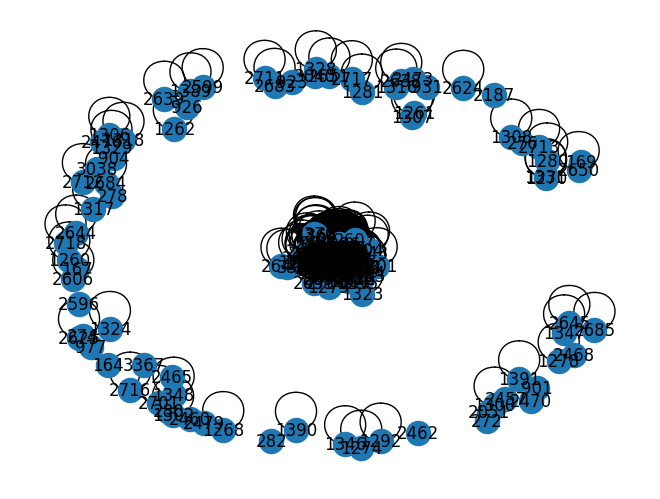
\includegraphics{Test_files/figure-pdf/cell-13-output-1.png}

}

\end{figure}

\bookmarksetup{startatroot}

\hypertarget{crawling-detik}{%
\chapter{Crawling Detik}\label{crawling-detik}}

\begin{Shaded}
\begin{Highlighting}[]
\ImportTok{import}\NormalTok{ requests }\ImportTok{as}\NormalTok{ req}
\ImportTok{import}\NormalTok{ pandas }\ImportTok{as}\NormalTok{ pd}
\ImportTok{from}\NormalTok{ bs4 }\ImportTok{import}\NormalTok{ BeautifulSoup }\ImportTok{as}\NormalTok{ bs}
\ImportTok{import}\NormalTok{ csv}

\NormalTok{header }\OperatorTok{=}\NormalTok{ \{}\StringTok{\textquotesingle{}user{-}agent\textquotesingle{}}\NormalTok{ : }\StringTok{\textquotesingle{}Mozilla/5.0 (Windows NT 10.0; Win64; x64) AppleWebKit/537.36 (KHTML, like Gecko) Chrome/109.0.0.0 Safari/537.36\textquotesingle{}}\NormalTok{\}}
\end{Highlighting}
\end{Shaded}

\begin{Shaded}
\begin{Highlighting}[]
\KeywordTok{def}\NormalTok{ scrap\_detik(link,hal,kategori):}
    \KeywordTok{global}\NormalTok{ header}
\NormalTok{    category }\OperatorTok{=}\NormalTok{ kategori}
\NormalTok{    data}\OperatorTok{=}\NormalTok{[]}
\NormalTok{    base\_url }\OperatorTok{=}\NormalTok{ link}
    \ControlFlowTok{for}\NormalTok{ page }\KeywordTok{in} \BuiltInTok{range}\NormalTok{(}\DecValTok{1}\NormalTok{,hal):}
\NormalTok{        url }\OperatorTok{=} \SpecialStringTok{f\textquotesingle{}}\SpecialCharTok{\{}\NormalTok{base\_url}\SpecialCharTok{\}}\SpecialStringTok{/}\SpecialCharTok{\{}\NormalTok{page}\SpecialCharTok{\}}\SpecialStringTok{\textquotesingle{}}
        \CommentTok{\# print(f"Judul: \{url\}")}
\NormalTok{        ge }\OperatorTok{=}\NormalTok{ req.get(url,header)}
        \ControlFlowTok{if}\NormalTok{ ge.status\_code }\OperatorTok{==} \DecValTok{200}\NormalTok{:}
\NormalTok{          soup }\OperatorTok{=}\NormalTok{ bs(ge.text, }\StringTok{\textquotesingle{}html.parser\textquotesingle{}}\NormalTok{)}
\NormalTok{          articles }\OperatorTok{=}\NormalTok{ soup.find\_all(}\StringTok{\textquotesingle{}article\textquotesingle{}}\NormalTok{, class\_}\OperatorTok{=}\StringTok{\textquotesingle{}list{-}content\_\_item\textquotesingle{}}\NormalTok{)}
          \ControlFlowTok{for}\NormalTok{ article }\KeywordTok{in}\NormalTok{ articles:}
\NormalTok{              link }\OperatorTok{=}\NormalTok{ article.find(}\StringTok{\textquotesingle{}a\textquotesingle{}}\NormalTok{)[}\StringTok{\textquotesingle{}href\textquotesingle{}}\NormalTok{]}
              \BuiltInTok{print}\NormalTok{(}\SpecialStringTok{f"Judul: }\SpecialCharTok{\{}\NormalTok{link}\SpecialCharTok{\}}\SpecialStringTok{"}\NormalTok{)}
\NormalTok{              title }\OperatorTok{=}\NormalTok{ article.find(}\StringTok{\textquotesingle{}h3\textquotesingle{}}\NormalTok{, class\_}\OperatorTok{=} \StringTok{\textquotesingle{}media\_\_title\textquotesingle{}}\NormalTok{).text.strip()}
\NormalTok{              content\_response }\OperatorTok{=}\NormalTok{ req.get(link)}
              \ControlFlowTok{if}\NormalTok{ content\_response.status\_code }\OperatorTok{==} \DecValTok{200}\NormalTok{:}
\NormalTok{                  content\_soup }\OperatorTok{=}\NormalTok{ bs(content\_response.text, }\StringTok{\textquotesingle{}html.parser\textquotesingle{}}\NormalTok{)}
\NormalTok{                  content }\OperatorTok{=}\NormalTok{ content\_soup.find(}\StringTok{\textquotesingle{}div\textquotesingle{}}\NormalTok{, class\_}\OperatorTok{=}\StringTok{\textquotesingle{}detail\_\_body{-}text\textquotesingle{}}\NormalTok{)}
                  \ControlFlowTok{if}\NormalTok{ content:}
\NormalTok{                      paragraphs }\OperatorTok{=}\NormalTok{ content.find\_all(}\StringTok{\textquotesingle{}p\textquotesingle{}}\NormalTok{)}
\NormalTok{                      article\_content }\OperatorTok{=} \StringTok{\textquotesingle{} \textquotesingle{}}\NormalTok{.join([p.text.strip() }\ControlFlowTok{for}\NormalTok{ p }\KeywordTok{in}\NormalTok{ paragraphs]).replace(}\StringTok{\textquotesingle{}}\CharTok{\textbackslash{}n}\StringTok{\textquotesingle{}}\NormalTok{, }\StringTok{\textquotesingle{}\textquotesingle{}}\NormalTok{).replace(}\StringTok{\textquotesingle{}ADVERTISEMENT\textquotesingle{}}\NormalTok{,}\StringTok{\textquotesingle{}\textquotesingle{}}\NormalTok{).replace(}\StringTok{\textquotesingle{}SCROLL TO RESUME CONTENT\textquotesingle{}}\NormalTok{,}\StringTok{\textquotesingle{}\textquotesingle{}}\NormalTok{)}
                      \CommentTok{\# print(f"Judul: \{title\}")}
                      \CommentTok{\# print(f"Isi Konten: \{article\_content\}")}
                      \CommentTok{\# print("{-}{-}{-}{-}{-}{-}{-}{-}{-}{-}{-}{-}")}
\NormalTok{                      data.append([title,article\_content,category])}
    \ControlFlowTok{return}\NormalTok{ data}
\end{Highlighting}
\end{Shaded}

\begin{Shaded}
\begin{Highlighting}[]
\NormalTok{edukasi }\OperatorTok{=}\NormalTok{ scrap\_detik(}\StringTok{\textquotesingle{}https://www.detik.com/edu/indeks\textquotesingle{}}\NormalTok{,}\DecValTok{1}\NormalTok{,}\StringTok{\textquotesingle{}Edukasi\textquotesingle{}}\NormalTok{)}
\NormalTok{finance }\OperatorTok{=}\NormalTok{ scrap\_detik(}\StringTok{\textquotesingle{}https://finance.detik.com/indeks\textquotesingle{}}\NormalTok{,}\DecValTok{1}\NormalTok{,}\StringTok{\textquotesingle{}Finance\textquotesingle{}}\NormalTok{)}
\NormalTok{sport }\OperatorTok{=}\NormalTok{ scrap\_detik(}\StringTok{\textquotesingle{}https://sport.detik.com/indeks\textquotesingle{}}\NormalTok{,}\DecValTok{1}\NormalTok{,}\StringTok{\textquotesingle{}Sport\textquotesingle{}}\NormalTok{)}
\NormalTok{food }\OperatorTok{=}\NormalTok{ scrap\_detik(}\StringTok{\textquotesingle{}https://food.detik.com/indeks\textquotesingle{}}\NormalTok{,}\DecValTok{1}\NormalTok{,}\StringTok{\textquotesingle{}Food\textquotesingle{}}\NormalTok{)}
\end{Highlighting}
\end{Shaded}

\begin{Shaded}
\begin{Highlighting}[]
\NormalTok{combined\_array }\OperatorTok{=}\NormalTok{ edukasi }\OperatorTok{+}\NormalTok{ finance }\OperatorTok{+}\NormalTok{ sport }\OperatorTok{+}\NormalTok{ food}
\BuiltInTok{print}\NormalTok{(combined\_array)}
\end{Highlighting}
\end{Shaded}

\begin{Shaded}
\begin{Highlighting}[]
\NormalTok{hasil }\OperatorTok{=}\NormalTok{ pd.DataFrame(combined\_array, columns}\OperatorTok{=}\NormalTok{[}\StringTok{\textquotesingle{}Judul\textquotesingle{}}\NormalTok{, }\StringTok{\textquotesingle{}Isi\textquotesingle{}}\NormalTok{, }\StringTok{\textquotesingle{}Kategori\textquotesingle{}}\NormalTok{])}
\NormalTok{df }\OperatorTok{=}\NormalTok{ hasil.sample(frac}\OperatorTok{=}\DecValTok{1}\NormalTok{).reset\_index(drop}\OperatorTok{=}\VariableTok{True}\NormalTok{)}
\NormalTok{df.to\_csv(}\StringTok{\textquotesingle{}/content/drive/MyDrive/ppw/ppw/crawling\_berita\_new.csv\textquotesingle{}}\NormalTok{, index}\OperatorTok{=}\VariableTok{False}\NormalTok{)}
\end{Highlighting}
\end{Shaded}

\begin{Shaded}
\begin{Highlighting}[]
\ImportTok{import}\NormalTok{ pandas }\ImportTok{as}\NormalTok{ pd}
\NormalTok{data }\OperatorTok{=}\NormalTok{ pd.read\_csv(}\StringTok{\textquotesingle{}/content/drive/MyDrive/ppw/ppw/crawling\_berita\_new.csv\textquotesingle{}}\NormalTok{)}
\NormalTok{data}
\end{Highlighting}
\end{Shaded}

\begin{longtable}[]{@{}llll@{}}
\toprule\noalign{}
& Judul & Isi & Kategori \\
\midrule\noalign{}
\endhead
\bottomrule\noalign{}
\endlastfoot
0 & Debut IMAG Sukses, KONI Pusat: Tahun Depan Leb... & Pekan Olahraga
Bela Diri Nasional atau Indones... & Sport \\
1 & Nikmati Pengalaman Santap Steak Lezat di Mad C... & Suasana yang
nyaman dengan makanan lezat, inil... & Food \\
2 & Arus Barang Impor Jadi Diperketat, Masa Transi... & Pemerintah terus
melakukan sejumlah upaya untu... & Finance \\
3 & Jorge Martin Promosi ke Ducati di 2024? & Rider Pramac Jorge Martin
muncul sebagai penan... & Sport \\
4 & Water Purifier Tenaga Surya Menangkan AHM Best... & Jakarta - PT
Astra Honda Motor menggelar AHM B... & Edukasi \\
... & ... & ... & ... \\
155 & Sempat Mangkrak, Proyek Tol Gilimanuk-Mengwi B... & Pemerintah
akan segera melelang ulang proyek T... & Finance \\
156 & Pahami Perbedaan Tekstil, Garmen, dan Konveksi & Bisnis pakaian
adalah salah satu bisnis yang s... & Finance \\
157 & Gado-gado Racikan Mak Gobang yang Terkenal di BSD & Jakarta - Gado
Gado Mak Gobang yang dulunya be... & Food \\
158 & Harta Karun Migas Papua Sudah Dilelang, Diinca... & Kementerian
Energi dan Sumber Daya Mineral (ES... & Finance \\
159 & Megawati Hangestri: Si Pevoli Viral Indonesia ... & Megawati
Hangestri Pertiwi terus menjadi perbi... & Sport \\
\end{longtable}

\hypertarget{crawling-pojok-baca}{%
\section{Crawling Pojok Baca}\label{crawling-pojok-baca}}

\begin{Shaded}
\begin{Highlighting}[]
\ImportTok{import}\NormalTok{ requests}
\ImportTok{from}\NormalTok{ bs4 }\ImportTok{import}\NormalTok{ BeautifulSoup}

\KeywordTok{def}\NormalTok{ scrape\_pojokbaca(link,hal,kategori):}
\NormalTok{    base\_url }\OperatorTok{=}\NormalTok{ link}
\NormalTok{    data }\OperatorTok{=}\NormalTok{ []}
    \ControlFlowTok{for}\NormalTok{ page\_number }\KeywordTok{in} \BuiltInTok{range}\NormalTok{(}\DecValTok{1}\NormalTok{, hal}\OperatorTok{+}\DecValTok{1}\NormalTok{):}
\NormalTok{        url }\OperatorTok{=} \SpecialStringTok{f\textquotesingle{}}\SpecialCharTok{\{}\NormalTok{base\_url}\SpecialCharTok{\}}\SpecialStringTok{?page=}\SpecialCharTok{\{}\NormalTok{page\_number}\SpecialCharTok{\}}\SpecialStringTok{\textquotesingle{}}
        \CommentTok{\# print(f"Scraping page: \{url\}")}

\NormalTok{        response }\OperatorTok{=}\NormalTok{ requests.get(url)}
        \ControlFlowTok{if}\NormalTok{ response.status\_code }\OperatorTok{==} \DecValTok{200}\NormalTok{:}
\NormalTok{            soup }\OperatorTok{=}\NormalTok{ BeautifulSoup(response.content, }\StringTok{\textquotesingle{}html.parser\textquotesingle{}}\NormalTok{)}
\NormalTok{            articles }\OperatorTok{=}\NormalTok{ soup.find\_all(}\StringTok{\textquotesingle{}div\textquotesingle{}}\NormalTok{, class\_}\OperatorTok{=}\StringTok{\textquotesingle{}latest\_\_item\textquotesingle{}}\NormalTok{)}

            \ControlFlowTok{for}\NormalTok{ article }\KeywordTok{in}\NormalTok{ articles:}
\NormalTok{                title }\OperatorTok{=}\NormalTok{ article.find(}\StringTok{\textquotesingle{}a\textquotesingle{}}\NormalTok{, class\_}\OperatorTok{=}\StringTok{\textquotesingle{}latest\_\_link\textquotesingle{}}\NormalTok{).text.strip()}
                \CommentTok{\# print(f"Title: \{title\}")}

\NormalTok{                content\_link }\OperatorTok{=}\NormalTok{ article.find(}\StringTok{\textquotesingle{}a\textquotesingle{}}\NormalTok{)[}\StringTok{\textquotesingle{}href\textquotesingle{}}\NormalTok{]}
                \CommentTok{\# print(f"Link: \{content\_link\}")}
\NormalTok{                content\_response }\OperatorTok{=}\NormalTok{ requests.get(content\_link)}

                \ControlFlowTok{if}\NormalTok{ content\_response.status\_code }\OperatorTok{==} \DecValTok{200}\NormalTok{:}
\NormalTok{                    content\_soup }\OperatorTok{=}\NormalTok{ BeautifulSoup(content\_response.content, }\StringTok{\textquotesingle{}html.parser\textquotesingle{}}\NormalTok{)}
\NormalTok{                    content }\OperatorTok{=}\NormalTok{ content\_soup.find(}\StringTok{\textquotesingle{}article\textquotesingle{}}\NormalTok{, class\_}\OperatorTok{=}\StringTok{\textquotesingle{}read\_\_content clearfix\textquotesingle{}}\NormalTok{)}

                    \ControlFlowTok{if}\NormalTok{ content:}
\NormalTok{                        paragraphs }\OperatorTok{=}\NormalTok{ content.find\_all(}\StringTok{\textquotesingle{}p\textquotesingle{}}\NormalTok{)}
\NormalTok{                        content\_text }\OperatorTok{=} \StringTok{\textquotesingle{} \textquotesingle{}}\NormalTok{.join([p.get\_text(strip}\OperatorTok{=}\VariableTok{True}\NormalTok{) }\ControlFlowTok{for}\NormalTok{ p }\KeywordTok{in}\NormalTok{ paragraphs]).replace(}\StringTok{\textquotesingle{}}\CharTok{\textbackslash{}n}\StringTok{\textquotesingle{}}\NormalTok{, }\StringTok{\textquotesingle{}\textquotesingle{}}\NormalTok{).replace(}\StringTok{\textquotesingle{}ADVERTISEMENT\textquotesingle{}}\NormalTok{,}\StringTok{\textquotesingle{}\textquotesingle{}}\NormalTok{).replace(}\StringTok{\textquotesingle{}SCROLL TO RESUME CONTENT\textquotesingle{}}\NormalTok{,}\StringTok{\textquotesingle{}\textquotesingle{}}\NormalTok{)}
                        \CommentTok{\# print(content\_text)}
\NormalTok{                        data.append([title,content\_text,kategori])}
    \ControlFlowTok{return}\NormalTok{ data}
\end{Highlighting}
\end{Shaded}

\begin{Shaded}
\begin{Highlighting}[]
\NormalTok{sport }\OperatorTok{=}\NormalTok{ scrape\_pojokbaca(}\StringTok{\textquotesingle{}https://www.pojokbaca.id/olahraga\textquotesingle{}}\NormalTok{, }\DecValTok{10}\NormalTok{,}\StringTok{\textquotesingle{}Sport\textquotesingle{}}\NormalTok{)}
\NormalTok{politik }\OperatorTok{=}\NormalTok{ scrape\_pojokbaca(}\StringTok{\textquotesingle{}https://www.pojokbaca.id/politik\textquotesingle{}}\NormalTok{,}\DecValTok{10}\NormalTok{,}\StringTok{\textquotesingle{}Politik\textquotesingle{}}\NormalTok{)}
\NormalTok{otomotif }\OperatorTok{=}\NormalTok{ scrape\_pojokbaca(}\StringTok{\textquotesingle{}https://www.pojokbaca.id/otomotif\textquotesingle{}}\NormalTok{,}\DecValTok{10}\NormalTok{,}\StringTok{\textquotesingle{}Otomotif\textquotesingle{}}\NormalTok{)}
\end{Highlighting}
\end{Shaded}

\begin{Shaded}
\begin{Highlighting}[]
\NormalTok{teknologi }\OperatorTok{=}\NormalTok{ scrape\_pojokbaca(}\StringTok{\textquotesingle{}https://www.pojokbaca.id/teknologi\textquotesingle{}}\NormalTok{,}\DecValTok{2}\NormalTok{,}\StringTok{\textquotesingle{}Teknologi\textquotesingle{}}\NormalTok{)}
\end{Highlighting}
\end{Shaded}

\begin{Shaded}
\begin{Highlighting}[]
\NormalTok{combined\_array }\OperatorTok{=}\NormalTok{ teknologi }\OperatorTok{+}\NormalTok{ politik }\OperatorTok{+}\NormalTok{ sport}
\BuiltInTok{print}\NormalTok{(combined\_array)}
\end{Highlighting}
\end{Shaded}

\begin{verbatim}
[['Strategi Sukses di Media Sosial, Ini Langkah-langkah Ampuh yang Patut Dicoba', ' POJOKBACA.ID -Dalam dunia bisnis modern,media sosialtelah menjadi salah satu sarana utama untuk melancarkan strategi pemasaran. Para pelaku bisnis, termasuk pelaku Usaha Mikro, Kecil, dan Menengah (UMKM) diIndonesia, semakin banyak mengandalkanmedia sosialsebagai alat untuk menjangkau target pasar mereka. Survei terbaru dari Hootsuite menunjukkan bahwa sekitar 58,4% populasi dunia saat ini menggunakanmedia sosial. Angka yang luar biasa ini membuktikan betapa pentingnya kehadiran bisnis di dunia maya. Tidak hanya itu, survei yang sama juga menunjukkan bahwa setiap penggunamedia sosialmenghabiskan sekitar 2,5 jam setiap harinya untuk berinteraksi di platform tersebut. Ini merupakan kesempatan emas yang tidak boleh dilewatkan oleh para pelaku bisnis untuk menjalin hubungan dengan audiens mereka. Dalam rangka memanfaatkan potensimedia sosialsecara maksimal, diperlukan rencana pemasaran yang matang dan terarah agar target bisnis dapat tercapai. Berikut ini adalah delapan langkah yang dapat kamu terapkan untuk membuat rencana pemasaranmedia sosialyang lebih efektif untuk bisnismu: 1. Menentukan Tujuan yang Jelas Sebelum memulai kampanye pemasaran dimedia sosial, kamu perlu menentukan tujuan yang jelas dan terukur. Apakah kamu ingin meningkatkan kesadaran merek, menarik lebih banyak pelanggan, atau meningkatkan penjualan? Dengan tujuan yang jelas, kamu dapat membuat strategi yang lebih efektif untuk mencapainya. 2. Mengidentifikasi Target Pasar Ketahui siapa target pasar atau audiens yang ingin kamu jangkau melaluimedia sosial. Kenali demografi, minat, dan kebutuhan mereka agar kamu dapat mengarahkan konten yang relevan dan menarik bagi mereka. Hal ini akan membantu meningkatkan interaksi dan keterlibatan dengan audiens. 3. Menyusun Konten Berkualitas Konten yang berkualitas tinggi adalah kunci keberhasilan dalam pemasaranmedia sosial. Buatlah konten yang informatif, menarik, dan bermanfaat bagi audiens. Gunakan berbagai format seperti gambar, video, dan artikel yang relevan dengan bisnismu. Jangan lupa untuk mengoptimalkan konten agar mudah ditemukan dan dibagikan oleh penggunamedia sosial. 4. Mempertimbangkan Konsistensi Branding Pastikan bahwa tampilan visual dan pesan yang kamu sampaikan melaluimedia sosialsesuai dengan branding bisnismu. Pilihlah warna, gaya, dan tone yang konsisten untuk membangun citra merek yang kuat dan mudah dikenali oleh audiens. Dengan konsistensi branding, kamu dapat memperkuat identitas bisnismu dimedia sosial.', 'Teknologi'], ['Terkait Pagu Indikatif Kemenpora TA 2024, Menpora Dito: Kita Kedepankan Akuntable dan Transparansi', ' JAKARTA, POJOKBACA.ID- Menteri Pemuda dan Olahraga Republik Indonesia (Menpora RI) Dito Ariotedjo mengikuti rapat kerja bersama Komisi X Dewan Perwakilan Rakyat Republik Indonesia (DPR RI) di Ruang RapatKomisi X DPR RI, Gedung Nusantara I, Kompleks Parlemen, Senayan, Jakarta, Jumat (9/6/2023). Rapat Kerja yang dipimpin KetuaKomisi X DPR RI, Syaiful Huda ini membahas Rencana Kerja dan Anggaran Kementerian Negara/Lembaga (RKA-K/L) dan Rencana Kerja Pemerintah (RKP) Kemenpora Tahun 2024. Dalam rapat kerja tersebut,Komisi X DPR RImenyetujui pagu indikatif Kemenpora RI pada RAPBN TA 2024 sebesar Rp 2.019.137.744.000. Atas persetujuan ini, Menpora Dito menyampaikan terima kasih kepadaKomisi X DPR RI. “Terima kasih kepada pimpinan dan anggotaKomisi X DPR RIyang sudah mempercayai Kementerian Pemuda dan Olahraga. Kami ucapkan terima kasih. Amanah ini akan dikerjakan dengan sebaik-baiknya,” kata Menpora Dito. Menpora Dito bilang, Kemenpora dalam hal ini akan terus menerapkan tranparansi dan akuntabel. “Pasti kita mengedepankan akuntabel dan transparansi dengan sebaik-baiknya,” sambungnya. Menpora Dito dalam pemaparan awalnya mengatakan ada beberapa program pemuda tangguh. Diantaranya membangun sarana prasarana Prestasi Hub yang dapat diakses individu/komunitas/organisasi kepemudaan dengan berbagai kegiatan peningkatan keterampilan dan perluasan jaringan di Aceh, Makassar, dan IKN. “Kemudin juga ada komunitas fest, pesta prestasi, Indonesian dream, muda berusaha, dan collab rangers,” jelas Menpora Dito. Disamping itu, juga ada sejumlah program olahraga maju. Misalnya sport industry summit, merdeka belajar kuliah merdeka, liga tarkam, dan membangun sport science institue di IKN, UNCEN, UI, dan UNSRI. “Lalu juga mengoptimalkan fasilitas olahraga di beberapa kampus untuk pengembangan atlet, membangun pusat pelatihan atlet nasional di Sumut, Sumsel, Papua, dan Solo. Serta menghidupkan kembali liga badminton dengan kelola olahraga dan manajemen profesional,” sambung Menpora Dito. Lebih lanjut, pada kesempatan ini, Menpora Dito mengusulkan tambahan anggaran pada pagu anggaran (sementara) 2024.Komisi X DPR RIpun menyetujui usulan tambahan pagu indikatif tersebut yakni Rp. 3.703.585.102.000. “Komisi X DPR menyetujui usulan pagu indikatif Kemenpora TA 2024 dan usulan penambahannya tersebut ke Badan Anggaran DPR RI,” Ketua Komisi X DPR Syaiful Huda. “Terkait usulan penambahan anggaran itu, Komisi X DPR mendorong Kemenpora untuk segera menyampaikan usulan tersebut kepada Bappenas, dan Kemenkeu disertai argumentasi yang kuat untuk mendukung program strategis dan rincian kegiatannya,” pungkasnya.***', 'Teknologi'], ['Datang ke Formula E, Anies Baswedan: Saya Beli Tiket Sendiri', 'JAKARTA, POJOKBACA.ID- Mantan Gubernur DKIJakarta,Anies Baswedan, hadir di acara balap mobil listrikFormula E2023 yang diadakan diJakartaInternational E-Prix Circuit (JIEC),Ancol,JakartaUtara pada Sabtu, 3 Juni 2023. Anies tiba bersama keluarganya, yaitu istrinya Fery Farhati, putrinya Mutiara Annisa Baswedan, dan menantunya Ali Saleh Alhuraiby. Saat tiba di pintu Bende sekitar pukul 12.17 WIB, Anies terlihat mengenakan baju bertuliskan "PesepedaJakarta" dengan logoJakarta+ Kota Kolaborasi. Setelah sampai di area pantai, Anies langsung dikelilingi oleh penontonFormula Eyang berbondong-bondong mengajaknya berfoto bersama. "Presiden 2024! Indonesia sejahtera," ujar salah satu pengunjung sambil berfoto dengan Anies. "Karena Pak Anies,Formula E2023 ada lagi," ujar yang lain. Terkait acara ini, Anies menyatakan bahwa ia membelitiketsecara mandiri. "Saya belitiket, saya bukan undangan. Saya membelitiketseperti orang lain juga," ungkap Anies kepada wartawan. Anies juga mengungkapkan kegembiraannya karenatiketFormula Eterjual habis. "Saya sangat senang bahwa tiketnya terjual habis. Semoga balapan berjalan lancar dan semua orang merasakan kebahagiaan serta membawa namaJakartadan Indonesia lebih baik," kata Anies. Formula EJakarta2023 dimulai pada Sabtu, 3 Juni 2023, diJakartaInternational E-Prix Circuit (JIEC),Ancol,JakartaUtara. Bagi para pemegangtiket, diharapkan untuk memperhatikan lokasi parkir kendaraan mereka. Terdapat dua kantong parkir resmi untuk penontonFormula EJakarta2023, yang dibagi berdasarkan kategoritiketFormula E. Informasi ini diunggah oleh akun InstagramFormula EJakarta@jakartaeprixofficial. Berikut adalah kantong parkir resmi untuk penontonFormula E2023: JakartaRoyal Suite 1ADrop off: GerbangAncolCarnaval JakartaDeluxe Suite 1BParkir:JakartaInternational Stadium (JIS) Grandstand dan Circuit FestivalLapangan Parkir Benyamin Sueb Formula EJakarta2023 dimulai dengan sesi latihan bebas kedua pukul 08.10-08.40 WIB. Kemudian dilanjutkan dengan sesi kualifikasi yang dijadwalkan berlangsung pukul 10.40-11.55 WIB. Pertandingan utama baru akan dimulai pukul 15.04 WIB.*** Sebelumnya, PTJakartaPropertindo (Jakpro) mengumumkan bahwa sekitar 40 ribu penonton diperkirakan akan meramaikan ajang balap mobil listrikFormula E2023 di JIECAncol.*** ', 'Teknologi'], ['Harganya Murah Pakai Banget, Ini 3 Pilihan Ponsel Terbaru 2023 yang Tak Boleh Dilewatkan!', ' POJOKBACA.ID- Tahun2023telah menghadirkan beragamponselterbaru yang dilengkapi dengan spesifikasi canggih. Bagi Anda yang menginginkanponseldengan harga terjangkau mulai dari Rp2 jutaan, berikut ini adalah tiga rekomendasiponselterbaru di tahun2023yang bisa Anda pertimbangkan. Pertama, hadir dengan keunggulan dalam segi performa dan kemampuan konektivitas, XiaomiRedmiNote 12 5G menjadi salah satu pilihan yang menarik.Ponselini memiliki layar luas berukuran 6,67 inci dengan resolusi 1.080 x 2.400 piksel. Tampilan yang jernih dan tajam akan memanjakan mata Anda saat menggunakanponselini. XiaomiRedmiNote 12 5G juga dibekali dengan RAM yang cukup besar, yaitu 4-8 GB, serta memori internal dengan kapasitas 128-256 GB. Dengan kapasitas baterai sebesar 5.000 mAh,ponselini mampu bertahan lama dalam penggunaan sehari-hari. Tidak hanya itu, kualitas kamera yang dimiliki juga tak kalah menarik dengan adanya kamera belakang beresolusi 48 + 8 + 2 MP dan kamera depan 13 MP yang akan menghasilkan foto yang memukau. Untuk memiliki XiaomiRedmiNote 12 5G ini, Anda perlu merogoh kocek sekitar Rp2.899.000. Kemudian, ada XiaomiPocoX5 yang juga menjadi salah satu pilihan menarik untuk Anda. Dengan layar 6,67 inci beresolusi 1.080 x 2.400 piksel,ponselini memberikan tampilan visual yang sangat memuaskan. XiaomiPocoX5 memiliki kualitas kamera yang tak kalah baik, dengan kamera belakang beresolusi 48 + 8 + 2 MP dan kamera depan 13 MP. Dengan dukungan RAM 4-6 GB dan memori internal 128-256 GB,ponselini mampu memberikan performa yang lancar dan penyimpanan yang cukup besar untuk kebutuhan pengguna. Diperkuat dengan baterai berkapasitas 5.000 mAh,ponselini juga dapat bertahan lama dalam penggunaan sehari-hari. XiaomiPocoX5 dibanderol dengan harga sekitar Rp3.299.000, yang membuatnya menjadi pilihan menarik di segmen harga ini. Selanjutnya, hadir dengan nama yang sudah tidak asing lagi,NokiaX30 adalahponselterbaru dariNokiayang patut dipertimbangkan.Ponselini memiliki baterai berkapasitas 4.200 mAh yang dapat memberikan daya tahan yang baik dalam penggunaan sehari-hari. NokiaX30 juga menghadirkan kualitas kamera yang menonjol, dengan kamera belakang beresolusi 50 + 13 MP dan kamera depan 16 MP. Hasil foto yang dihasilkan akan memukau dan memperindah momen-momen berharga Anda. Untuk memilikiNokiaX30 ini, Anda perlu mengeluarkan kocek sekitar Rp3.599.000. Demikianlah tiga pilihanponselterbaru di tahun2023dengan harga mulai dari Rp2 jutaan. Setiapponselmemiliki keunggulan dan fitur menarik yang dapat sesuai dengan kebutuhan dan preferensi pengguna. Tentukan pilihan Anda dan dapatkan pengalaman menggunakanponselyang optimal sesuai dengan budget yang dimiliki. Selamat memilih!***', 'Teknologi'], ['Oppo Find N2 Flip dan Samsung Z Flip 4,  Berbedaan Performa dan Fitur Unggulan Dua Ponsel Lipat Ini!', ' POJOKBACA.ID -Industri smartphone terus mengalami kemajuan pesat dengan penemuan dan inovasi baru yang mengagumkan. Salah satu terobosan terbaru yang sedang menjadi sorotan adalahponsellipat. OppodanSamsung, dua raksasa teknologi, telah meluncurkanponsellipat terbaru mereka, yaituOppoFind N2FlipdanSamsungZFlip4. Kedua perangkat ini menawarkan model lipat yang menarik dengan spesifikasi hardware yang canggih. Dalam artikel ini, kita akan menjelajahi skor Antutu, performa, uji game, danbateraidari keduaponsellipat ini. Find N2Flip, yang merupakan produk terbaru dariOppodi Indonesia, memiliki desain yang menarik dengan model lekukan yang mirip dengan kulit kerang. Perlu dicatat bahwaOppoFind N2Flipmemiliki kemiripan dengan Galaxy ZFlip4 dariSamsung, terutama dalam hal model lipatannya. Menariknya, harga keduanya sama persis, yaitu Rp 15 juta untuk varian 8 GB/256 GB.OppoFind N2Flipditenagai oleh chipset kelas atas Mediatek Dimensity 9000 Plus, sementaraSamsungGalaxy ZFlip4 menggunakan Qualcomm Snapdragon 8 Plus Gen 1. Spesifikasi hardware inti keduaponselini dapat dilihat dalam tabel di bawah ini: Spesifikasi hardware: 1.OppoFind N2Flip: -Chipset: Mediatek Dimensity 9000 Plus (4 nm)-Prosesor (CPU): Octa-core (1x3.20 GHz Cortex-X2 & 3x2.85 GHz Cortex-A710 & 4x1.80 GHz Cortex-A510)-Pengolah Grafis (GPU): Mali-G710 MC10-RAM: 8 GB LPDDR5-Storage: 256 GB UFS 3.1-Baterai: 4.300 mAh (SuperVOOC 44W via kabel) 2.SamsungGalaxy ZFlip4: -Chipset: Qualcomm Snapdragon 8 Plus Gen 1 (4 nm)-Prosesor (CPU): Octa-core (1x3.19 GHz Cortex-X2 & 3x2.75 GHz Cortex-A710 & 4x1.80 GHz Cortex-A510)-Pengolah Grafis (GPU): Adreno 730-RAM: 8 GB LPDDR5-Storage: 128 GB/256 GB/512 GB UFS 3.1-Baterai: 3.700 mAh (Fast Charging 25W via kabel, 15W via nirkabel) Saat dilakukan sejumlah pengujian menggunakan aplikasi benchmark populer seperti Antutu (versi 9), Geekbench (versi 6), PCMark, dan 3DMark pada keduaponselini.Hasilnya,OppoFind N2Flipmemiliki skor performa Antutu yang lebih tinggi dibandingkanSamsungGalaxy ZFlip4, dengan selisih yang tidak terlalu signifikan. Skor AntutuOppoFind N2Flipadalah 759.140 poin, sedangkanSamsungGalaxy ZFlip4 mencetak skor 717.167 poin. Pada platform Geekbench 6, kinerja CPUOppoFind N2Flipjuga lebih tinggi dengan skor performa single core sebesar 1.164 poin dan multi core sebesar 3.032 poin. Di sisi lain,SamsungGalaxy ZFlip4 mencetak skor performa single core sebesar 1.145 poin dan multi core sebesar 2.931 poin. Ketika menguji kinerja grafis,OppoFind N2Flipsedikit unggul dengan skor performa 3DMark mode "Wild Life" sebesar 7.361 poin dan frame rate rata-rata 44,10 FPS. Sementara itu,SamsungGalaxy ZFlip4 mencetak skor performa 3DMark mode "Wild Life" sebesar 6.483 poin dengan frame rate rata-rata 38,80 FPS.', 'Teknologi'], ['Menjajal Kamera 200 MP Samsung Galaxy S23 Ultra di Konser Suga BTS: Hasilnya Mencengangkan!', ' JAKARTA, POJOKBACA.ID- Dalam konser solo bertajuk "Suga| D Agust in Jakarta" yang digelar di ICE BSD, Tangerang selama tiga hari pada 26—28 Mei 2023,SugaBTSatau yang dikenal dengan nama Agust D telah menyuguhkan penampilan yang memukau. Sebagai salah satu penggemar setiaBTS,\xa0para Fans tentu\xa0tidak melewatkan kesempatan untuk hadir dalam konser tersebut pada hari pertama, Jumat (26/5/2023) yang lalu. Tak hanya itu, kami juga membawaSamsungGalaxy S23 Ultra, smartphone terbaru dengan fitur kamera unggulan, untuk mengabadikan momen berharga tersebut. Dengan durasi konser yang berlangsung selama dua jam, dari pukul 19.00 hingga 21.00 WIB, KompasTekno menguji kebolehan sejumlah fitur kameraSamsungGalaxy S23 Ultra, termasuk kamera utama yang memiliki resolusi mencapai 200 MP. Perlu diketahui, Galaxy S23 Ultra merupakan perangkat pertama dariSamsungyang menghadirkan kamera dengan resolusi sebesar itu. Tidak hanya itu, fitur telefoto zoom optik 100x pada kamera tersebut memungkinkan pengguna untuk mengabadikan aksiSugaBTSdi atas panggung dengan jelas dan dekat. Berdasarkan pengalaman KompasTekno dalam menjajal fitur-fitur tersebut, hasil foto yang dihasilkan oleh kamera 200 MP Galaxy S23 Ultra terlihat sangat mengesankan. Foto-foto tersebut memiliki kontras yang tajam, saturasi warna yang tinggi namun tidak berlebihan, serta hampir tidak terlihat adanya bintik warna (noise). Bahkan, ketika foto tersebut diperbesar, kualitasnya tetap terjaga tanpa adanya kehilangan detail yang signifikan. Hal ini bisa dimaklumi mengingat resolusi gambar yang dihasilkan oleh kamera 200 MP jauh lebih besar dibandingkan dengan kamera ultrawide 12 MP. Sebagai perbandingan, resolusi foto dari kamera 200 MP mencapai 16.620x12.240 (3:4) piksel dengan ukuran file sebesar 22,75 MB, sementara kamera 12 MP hanya memiliki resolusi 4.000x3.000 piksel dengan ukuran file 2,44 MB. Perbedaan resolusi dan ukuran yang signifikan ini menjadikan foto dari kamera 12 MP lebih cenderung pecah ketika diperbesar. Dalam konteks penggunaan sehari-hari, fitur kamera 200 MP padaSamsungGalaxy S23 Ultra sangat direkomendasikan untuk mengabadikan suasana keramaian di tempat-tempat yang ramai. Dalam konserSugaBTSdi ICE BSD, misalnya, pengguna smartphone ini dapat dengan mudah mengambil gambar dari jarak jauh dengan hasil yang jernih dan detail yang tajam. Anda tidak perlu khawatir akan kehilangan momen penting meskipun berada di belakang kerumunan, karena fitur telefoto zoom optik 100x pada Galaxy S23 Ultra mampu memberikan jarak pandang yang lebih dekat secara visual. Tentu saja, dalam hal penggunaan kamera, selain spesifikasi teknis yang canggih, kemampuan fotografer dalam mengambil gambar juga turut berperan penting. Namun, dengan kameraSamsungGalaxy S23 Ultra yang memiliki kemampuan unggulan, seperti resolusi tinggi dan fitur zoom optik yang memukau, siapa pun dapat dengan mudah menghasilkan foto-foto berkualitas tinggi tanpa perlu keahlian khusus dalam fotografi. Melalui pengalaman KompasTekno dalam menjajal kebolehan kameraSamsungGalaxy S23 Ultra di konserSugaBTSdi Jakarta, Jumat (26/5/2023) kemarin, dapat disimpulkan bahwa smartphone ini mampu memberikan pengalaman fotografi yang memuaskan. Dengan resolusi kamera 200 MP yang luar biasa dan kemampuan zoom optik 100x, pengguna dapat mengabadikan momen-momen berharga dengan jelas dan detail yang tajam.SamsungGalaxy S23 Ultra menjadi pilihan yang tepat bagi mereka yang menginginkan hasil foto berkualitas tinggi dalam berbagai situasi, termasuk dalam suasana keramaian di konser-konser yang memukau seperti "Suga| D Agust in Jakarta".*** Sumber: Kompas', 'Teknologi'], ['Cara Edit Transisi di CapCut TikTok agar Video Semakin Menarik', ' POJOKBACA.ID- Untuk membuatvideokonten diTikTokmenjadi lebih menarik, tentu kreativitas dalam mengedit dibutuhkan. Salah satu bagian pengeditanvideoyang memberikan efek menarik adalah menambahkan unsur transisi. Transisivideomerupakan efek visual yang terjadi saat berpindah satuvideokevideoberikutnya. Transisi ini akan menimbulkan efek menarik dan unik saat Anda ingin menggabungkan duavideobersamaan. Adapun salah satu aplikasieditvideoyang menyediakan template transisi beragam ada di aplikasiCapCut. CapCutmemiliki banyak jenis transisi unik dan menarik yang bisa Anda gunakan untuk mempercantik kontenvideoAnda diTikTok. Lantas bagaimana caraedittransisi diCapCut? Selengkapnya berikut ini langkah-langkahnya. Caraedittransisi diCapCutTikTok 1. Buka aplikasiCapCut.2. Pilih "Proyek baru".3. Nantinya Anda akan menuju bagian pengeditanvideo.4. Klik pada bagian potonganvideo.5. Nantinya akan muncul beragam pilihan template transisi yang bisa Anda pilih sesuai kehendak.6. Anda dapat mengatur durasi transisi yang ingin digunakan.7. Apabila ingin menggunakan template transisi yang sama, maka klik "Terapkan ke semua".8. Namun jika Anda ingin menggunakan template berbeda untuk bagian potonganvideolain, cukup klik centang dan beralih ke bagian potonganvideolain.9. Kemudian pilih transisivideoyang Anda inginkan.10. Jika pengeditanvideotelah selesai, maka klik tanda panah ke atas.11.Videoakan diekspor dan siap Anda unggah di berbagai media sosial. Itulah caraedittransisi diCapCut. Selain mengedit transisi, diCapCutAnda juga bisa mengeditvideodan foto dalam satu frame. Adapun tutorialnya bisa Anda simak di panduan "Cara Menggabungkan Foto danVideodiCapCutdalam Satu Frame". Selamat Mencoba!***', 'Teknologi'], ['Review Samsung Galaxy A54 5G, HP Kelas Menengah Rasa Flagship', ' JAKARTA, POJOKBACA.ID -SamsungGalaxyA54 5G, sebuah ponsel kelas menengah dengan rasa flagship, telah hadir diIndonesiasejak bulanMaretlalu. Dalam menghadirkan produk terbarunya ini, Samsung menitikberatkan pada aspek kamera dan desain yang mengadopsi gaya ponsel flagship. Setelah menggunakan SamsungGalaxyA54 5G selama satu bulan dengan harga Rp 6,4 juta, mari kita simak ulasan lengkapnya. Berikut ini adalah ulasan SamsungGalaxyA54 5Gvarianwarna Awesome Lime (8 GB/256 GB) yang tersedia di pasar ritelIndonesia: Bila kita melihat isi kotak penjualan SamsungGalaxyA54 5G, kita akan menemukan bahwa isi kemasannya sangat minimalis. Di dalamnya terdapat satu unit ponsel, kabel USB C to USB C, SIM card ejector tool, panduan pengguna, serta kartu garansi. Dalam hal kemasan, SamsungGalaxyA54 5G masih menggunakan desain kotak yang sama dengan pendahulunya. Kemasan tersebut didominasi oleh warna putih dengan foto produk yang memperlihatkan desain layar dan bagian belakangSamsung A54 5G. Meskipun begitu, Samsung tidak menyertakan aksesori adapter (kepala) charger di dalam kotak penjualanGalaxyA54 5G. Namun, pengguna masih bisa menggunakan charger HP Samsung lamanya atau membeli adapter Super Fast Charger 25 watt secara terpisah. Yang paling mencolok dari SamsungGalaxyA54 5G adalah perubahan desain pada bagian belakangnya yang kini menyerupai ponsel flagshipGalaxyS23. Terdapat tiga kamera yang disusun secara vertikal tanpa modul kamera pada bagian belakang SamsungGalaxyA54. Lensa-lensa tersebut dikelilingi oleh cincin berbahan metal, menciptakan tampilan yang mirip denganGalaxyS23. Selain itu, ponsel ini juga menggunakan material kaca Gorilla Glass 5 untuk punggungnya, memberikan finishing glossy yang mengkilap dengan efek cermin. Dengan dimensi 158,2 x 76,7 x 8,2 mm dan berat 202 gram, SamsungGalaxyA54 terasa nyaman dan kompak saat digenggam. Namun, punggung ponsel ini agak licin, sehingga disarankan untuk menggunakan soft case atau hard case tambahan untuk keamanan. Layar SamsungGalaxyA54 memiliki panel Super AMOLED seluas 6,4 inci dengan resolusi Full HD Plus dan rasio aspek 19,5:9. Layar tersebut juga dilengkapi dengan refresh rate 120 Hz, sehingga memberikan pengalaman yang mulus dan lancar saat menjelajah menu dan aplikasi. Menonton video atau film juga menjadi lebih memuaskan. Selain itu, tingkat kecerahan layarnya mencapai 1.000 nits, 25 persen lebih terang dariGalaxyA53. Dengan kecerahan yang lebih tinggi ini, layar SamsungGalaxyA54 tetap dapat terbaca dengan baik di bawah sinar matahari. Keberadaan panel Super AMOLED juga memungkinkan adanya pemindai sidik jari di bawah layar.***  ', 'Teknologi'], ['Dibalik Kerlap Kerlip Lampu dan Nyanyian Dangdut, Apa yang Sebenarnya Terjadi di Kandeman Batang?', ' BATANG, POJOKBACA.ID- Wilayah Kandeman, Batang, Jawa Tengah, telah menjadi sorotan pada malam-malam sekarang ini. Suasana di sepanjang Jalan Raya Batang begitu hidup dengan kerlap kerlip lampu yang temaram dan irama dangdut yang bergema. Namun, di balik hingar bingar itu, tersembunyi sebuah fenomena sosial yang mengundang perhatian publik. Warung-warung di sepanjang jalur ini menjadi saksi bisu keberadaan sebuah tempat yang tidak terduga, tempat di mana para pekerja seks meramaikan suasana. Wanita-wanita dengan penampilan yang seronok menghiasi warung-warung itu, menemani para sopir truk yang singgah sejenak. Mereka mengenakan pakaian yang mengundang perhatian, seperti pakaian pendek dan celana jeans yang menyoroti keindahan paha mereka. Bahkan, baju mereka begitu ketat dan memamerkan belahan dadanya. Usia mereka berkisar antara 20 hingga 40 tahun. Mereka adalah pekerja seks yang bekerja di tempat-tempatprostitusisemacamwarung remang-remangyang beberapa waktu lalu menjadi viral dan menarik perhatianLSMserta masyarakat setempat. Pada Jumat, 19 Mei 2023, masalah ini diadukan oleh sejumlahLSMkepadaDPRDBatang. Kawasan ini kini berubah menjadi salah satu lokalisasi paling ramai di jalur Pantai Utara, yang dikenal dengan sebutan Pantura. Terdapat tidak kurang dari 30 warung yang berjejer sepanjang 100 meter. Di sinilah para pengunjung dapat menikmati minuman ringan, kopi, bir, layanan pijat, dan hiburan dari perempuan-perempuan yang siap menghibur. "Perempuan yang berdandan pasti selalu mendapat pasangan," ujar Toto, seorang sopir truk yang telah lama melintas di jalur ini. Untuk sekali kencan, mereka menetapkan harga sekitar Rp200 hingga 300 ribu. Hampir semua pelanggan yang mereka layani adalah sopir truk yang mampir sejenak. Toto bahkan berbangga diri karena selalu mendapatkan tarif paling murah, sebab ia adalah pengunjung tetap di tempat tersebut. "Ada sebuah kamar kecil yang disediakan di belakang warung," bisiknya dengan seringai. Berdasarkan wawancara dan investigasi yang dilakukan, terlihat jelas bahwa keberadaan tempat tersebut telah menjadi fenomena yang mengundang perbincangan di masyarakat. Pendapat pun bermacam-macam. Terdapat suara yang mempertanyakan moralitas dan dampak sosial yang ditimbulkan oleh keberadaan tempat semacam ini. Masyarakat Mengadu keDPRD Audiensi masyarakat Batang dengan DPRD terkait maraknya prostitusi di Kandeman. (Foto: Humas DPRD) Puluhan warga Desa/Kecamatan Kandeman, Kabupaten Batang, Jumat 19 Mei 2023 mendatangi gedungDPRDsetempat. Kedatangan mereka untuk mendesak agarwarung remang-remangyang ada di tepi jalur Pantura wilayah desanya agar ditertibkan dan dibongkar, karena telah dipergunakan sebagai tempatprostitusiterselubung berkedok warung makan. Dihadapan Komisi BDPRDBatang, warga mendesak agarwarung remang-remangyang ada di wilayahnya untuk ditertibkan dan dibongkar. Selain itu, warga juga mendesak agar adanya tindakan tegas terhadap pelakuprostitusiyang berkedok warung kopi dan warung makan. "Kami minta dilakukan penertiban dan pembongkaranwarung remang-remang, serta sanksi tegas pada pelakuprostitusidi tempat tersebut," tegas Bambang, perwakilan warga saat audiensi dengan Komisi BDPRDBatang, Jumat 19 Mei 2023. Selain tindakan tegas, Bambang juga mendesak agar dilakukan pemeriksaan rutin pada pelakuprostitusiusai dilakukan penertiban. Warga juga berharap agar Pemkab bisa mencarikan bagi mantan pekerja seks komersial dan pemilik warung usai dilakukan penertiban. "Kami sebelumnya sudah sudah melakukan kajian terlebih dahulu terkait adanya praktekprostitusiyang dilakukan diwarung remang-remangyang berada di tepi jalur Pantura Kandeman. Hasilnya, ternyata memang ada praktikprostitusi, sehingga kami mendesak untuk ditertibkan dan dibongkar," jelas Bambang. Bambang mengungkapkan, sebelumnya warung-warung yang berada di sepanjang jalur Pantura, tepatnya bawah flay over jalan tim dulunya hanya menjual makanan dan minuman saja. Namun kini ternyata juga menyediakan layananprostitusibagi para orang yang datang. "Pemilik warung kini sengaja menyediakan kamar yang digunakan untuk praktekprostitusi. Hal itu menunjukan bahwa warung-warung tersebut telah menyimpang, karena menyediakan layananprostitusi," papar Bambang. Padahal, lanjut Bambang, Kabupaten Batang mempunyai Peraturan Daerah (Perda) yang melarang adanya kegiatanprostitusidi wilayahnya, yaitu Perda Nomor 6 Tahun 2011 tentang pemberantasan pelacuran di wilayah Kabupaten Batang. Sehingga apa yang dilakukan pemilik warung jelas-jelas melanggar, sehingga harus dilakukan penertiban. "Warung-warung tersebut juga dibangun di atas tanah drainase jalan milik Kementerian PUPR, sehingga mendesak harus dilakukan penertiban," tambang Bambang. Adanya praktikprostitusidiwarung remang-remangitu juga dibenarkan oleh Camat Kandeman, M. Kusrin yang hadir pada audensi tersebut. Bahkan pihaknya sudah melakukan pendataan pemilik warung, termasuk pekerja seks komersial yang ada di sana. Selain itu, juga sudah pernah dilakukan rapat koordinasi dengan instansi terkait lainnya. "Memang ada praktikprostitusidi sana. Kami telah melakukan rapat koordinasi dan pendataan warung yang ada di sepanjang tapi jalur Pantura mulai dari ujung timur hingga depan Kantor Kecamatan Kandeman sejak 2021," ujar Kusrin.', 'Teknologi'], ['Ternyata Cuma 4 Merek Smartphone Ini yang Jadi Favorit Orang Amerika', ' POJOKBACA.ID -Apple tetap menjadi merek smartphone yang paling disukai oleh orangAmerikaSerikat (AS), menurut riset yang dilakukan oleh American Customer Satisfaction Index (ACSI). Riset tahun ini menunjukkan bahwa Apple berhasil meraih skor yang lebih tinggi dibanding tahun sebelumnya, dengan skor 81/100 dibandingkan dengan 80/100 pada tahun sebelumnya. Hal ini menunjukkan bahwa konsumen menganggap performa Apple lebih baik. Selain Apple, merek smartphone lain yang populer di kalangan konsumen AS adalahSamsung. SkorSamsungdalam riset ACSI 2022-2023 tetap sama dengan skor tahun lalu, yaitu 80/100. Namun, jika dibandingkan dengan Apple, sentimen konsumen AS terhadap Apple sedikit lebih kuat daripadaSamsung. Selain Apple danSamsung, Google juga muncul dalam daftar merek smartphone favorit di AS. Pada tahun ini, Google meraih skor 78/100, meningkat 1 persen dibandingkan tahun sebelumnya (77/100). ACSI menyebut bahwa jika Google dapat mempertahankan performanya, kemungkinan skornya akan sama denganSamsungpada tahun depan. Namun, Motorola mengalami penurunan skor sebesar 3 persen dari 77/100 tahun lalu menjadi 75/100. Demikian pula, merek-merek "Lainnya" yang termasuk TCL, OnePlus, dan Nokia mengalami penurunan skor dari 74/100 menjadi 71/100. ACSI juga menyertakan indeks kepuasan smartphone 5G dalam laporan tahun ini. Hasilnya menunjukkan bahwa pengguna ponsel di AS cenderung puas dengan smartphone 5G dibandingkan dengan yang tidak memiliki fitur 5G, dengan skor 80 dari skala 100. Apple danSamsungmeraih skor tertinggi dalam aspek kepuasan konsumen terhadap smartphone 5G, keduanya dengan skor 81/100. Google mendapatkan skor 80/100 dan Motorola 76/100. Riset ACSI dilakukan dari April 2022 hingga Maret 2023 dengan melibatkan survei dari 15.881 konsumen yang dipilih secara acak dan dihubungi melalui email.*** ', 'Teknologi'], ['Ini Cara dan Syarat Perpanjang SIM Secara Online 2023', " JAKARTA, POJOKBACA.ID -Surat Izin Mengemudi atauSIMmerupakan bukti registrasi dan identifikasi yang diberikanPolrisebagai salah satu syarat berkendara.SIMdi Indonesia punya ketentuan tidak berlaku seumur hidup, dan pemegangnya harus memperpanjang masa berlaku setiap lima tahun sekali. Saat ini Anda tidak hanya bisa memperpanjangSIMdi Satpas ataupun geraiSIMkeliling. Di eradigitalini, Anda bisa memperpanjangSIMsecaraonline. Selain itu, pengendara perlu mengetahui tarif resmi perpanjanganSIMagar tidak ditipu oleh oknum yang menawarkan jasa pengurusan dokumen tersebut secara instan alias calo. Tarif perpanjanganSIMtercantum dalam Peraturan Pemerintah (PP) Nomor 76 Tahun 2020 tentang Jenis dan Tarif atas Jenis Penerimaan Negara Bukan Pajak yang Berlaku pada Kepolisian Negara Republik Indonesia. Pasal 1 peraturan tersebut menyatakan penerbitan perpanjanganSIMmerupakan bagian dari Penerimaan Negara Bukan Pajak (PNBP) di Kepolisian. Oleh karena itu, besaran tarif perpanjanganSIMsudah ditetapkan lewat ketentuan peraturan perundang-undangan dan mendapat persetujuan Menteri Keuangan. Syarat perpanjanganSIMonline Untuk memperpanjangSIMsecaraonline, Anda perlu menyiapkan dokumen-dokumen sebagai syarat: SIMlamaKartu Tanda Penduduk (KTP)Hasil RIKKES JasmaniHasil tes psikologiPas foto dengan latar biru, bukan selfieFoto tanda tangan di atas kertas putih polos dengan tinta tebalPerpanjangan dilakukan 90 hari sebelum masa berlaku habisCara perpanjangSIMonline Anda bisa memperpanjangSIMmelalui aplikasiDigitalKorlantasPolri. Berikut caranya: 1. Unduh aplikasiDigitalKorlantasPolridi Google Play Store2. Registrasi dengan nomor handphone untuk mendapatkan OTP3. Masukkan kode OTP4. Buat PIN dan konfirmasi ulang PIN5. Masukkan data profil mulai dari NIK, nama, dan email6. Periksa notifikasi pengaktifan akun di email, kemudian aktifkan7. Verifikasi KTP dengan fitur foto liveness8. Lakukan tes pemeriksaan kesehatan atau RIKKES Jasmani di erikkes.id di browser hp9. Lakukan tes psikologi di app.eppsi.id di browser hp10. Lakukan perpanjanganSIMonlinemelalui 'MenuSIM', lalu 'PerpanjanganSIM'11. Unggah dokumen syarat perpanjanganSIMonline12. Pilih Satpas penerbitSIM13. Masukkan nomor rekening Anda14. Pilih metode pengiriman melalui Pos Indonesia ke alamat Anda atau metode pengambilan di Satpas penerbit15. Pilih metode pembayaran dan sertakan nomor rekning16. Selesaikan pembayaran nontunai sesuai prosedur17. Periksa status transaksi di 'Menu Transaksi'18. Sistem akan memproses dan mengirimSIMjika sudah selesai diperpanjang19. Tarif resmi perpanjanganSIM2023 Berikut ini adalah tarif resmi perpanjanganSIMberdasarkan kategori jenisSIM: -PerpanjanganSIMA: Rp80 ribu per penerbitan-PerpanjanganSIMBI: Rp80 ribu per penerbitan-PerpanjanganSIMBII: Rp80 ribu per penerbitan-PerpanjanganSIMC: Rp75 ribu per penerbitan-PerpanjanganSIMCI: Rp75 ribu per penerbitan-PerpanjanganSIMCII: Rp75 ribu per penerbitan-PenerbitanSIMD: Rp30 ribu per penerbitan-PenerbitanSIMDI: Rp30 ribu per penerbitan-PembuatanSIMInternasional: Rp225 ribu per penerbitan-Biaya tes psikologi: Rp37.500-Biaya RIKKES Jasmani: Sesuai kebijakan tarif klinik yang dipilih Dengan adanya layanan perpanjanganSIMsecaraonline, pengendara dapat memperpanjangSIMdengan lebih mudah dan efisien. Namun, penting untuk selalu memperhatikan ketentuan dan persyaratan yang telah ditentukan, serta menggunakan aplikasi resmi yang disediakan olehDigitalKorlantasPolri. PerpanjanganSIMsecaraonlinememberikan kemudahan bagi pemegangSIMdalam melaksanakan proses perpanjangan tanpa harus datang langsung ke Satpas. Pastikan Anda memenuhi semua syarat dan mengikuti langkah-langkah dengan seksama agar proses perpanjanganSIMberjalan lancar. DenganSIMyang selalu terperbaharui, pengendara dapat tetap mematuhi peraturan lalu lintas dan menjaga keamanan berkendara.***", 'Teknologi'], ['Ancaman Penjahat Siber: Jangan Sampai Terjebak, Hapus Segera 19 Aplikasi Berbahaya dari HP Anda!', ' JAKARTA, POJOKBACA.ID -Penjahatsibersemakin kreatif dalam mencari cara untuk melanggar privasi dan keamanan pengguna. Salah satu metode yang sering mereka gunakan adalah melalui serangkaianaplikasiberbahaya yang tersedia di Google Play Store. Menurut laporan dari MalwareFox, Android menjadi target utama para penyerangsiberuntuk melakukan kegiatan ilegal. Hal ini dikarenakan Android merupakan sistem operasi yang open-source, sehingga memungkinkan untuk disesuaikan dengan kebutuhan, berbeda dengan sistem operasi iOS. "Mudah bagipenjahatsiberuntuk menyusup ke perangkat Android melaluiaplikasiberbahaya, seperti Trojan, Adware, Spyware, Keylogger, dan lainnya," tulis laporan tersebut. Dilansir dari Hindustan Times, berikut adalah daftaraplikasiberbahaya yang harus segera dihapus dari perangkatHPAnda. Pastikan tidak ada satu pun dariaplikasi-aplikasiini yang masih terpasang diHPAnda! 1. Fare Gamehub and Box (Trojan)2. Hope Camera-Picture Record (Trojan)3. Same Launcher and Live Wallpaper (Trojan)4. Amazing Wallpaper (Trojan)5. Cool Emoji Editor and Sticker (Trojan)6. Simple Note Scanner (Spyware)7. Universal PDF Scanner (Spyware)8. Private Messenger (Spyware)9. Premium SMS (Spyware)10. Blood Pressure Checker (Spyware)11. Cool Keyboard (Spyware)12. Paint Art (Spyware)13. Color Message (Spyware)14. Vlog Star Video Editor (Malware)15. Creative 3D Launcher (Malware)16. Wow Beauty Camera-Picture (Malware)17. Gif Emoji Keyboard (Malware)18. Instant Heart Rate Anytime (Malware)19. Delicate Messenger (Malware) Penting untuk segera menghapusaplikasi-aplikasitersebut agar tidak terjadi pencurian data pribadi, penggunaan informasi secara ilegal, atau kerentanan terhadap serangansiberlainnya. Selalu pastikan untuk hanya mengunduhaplikasidari sumber yang terpercaya, dan lakukan pembaruan sistem secara teratur guna menjaga keamanan perangkat Anda.***  ', 'Teknologi'], ['Bumi Diklaim Aman dari Tabrakan Asteroid, Tapi Sampai Kapan?', ' JAKARTA, POJOKBACA.ID -Sebuah studi terbaru tentang orbit objek luar angkasa telah menemukan bahwaBumiaman daritabrakanasteroidsetidaknya dalam rentang waktu sekitar 1.000 tahun ke depan. NASAdan observatorium lainnya secara terus-menerus melacak orbit objek-objek yang ditemukan di Tata Surya, terutama fokus pada "objek dekatBumi" (Near Earth Object/NEO) dengan diameter 140 meter atau lebih besar yang berpotensi mengakibatkan kehancuran jika terjaditabrakandenganBumi. Dengan mempelajari orbitnya, para ahli astrofisika dapat memperkirakan orbit objek tersebut di masa depan dan memprediksi apakah objek tersebut berada dalam jangkauan Tata Surya kita. Hingga saat ini, para astronom telah mampu memprediksi orbit objek-objek yang diketahui hingga sekitar 100 tahun ke depan. Berita baiknya, menurut studi tersebut, tidak adaasteroidyang diketahui memiliki diameter lebih dari 140 meter dan memiliki kemungkinan signifikan untuk menabrakBumidalam 100 tahun ke depan, menurutNASA. Sumber lain melaporkan informasi yang lebih menggembirakan. Tim yang dipimpin oleh Oscar Fuentes-Muñoz dari University of Colorado Boulder bahkan dapat memprediksi jalurasteroidyang lebih besar hingga 1.000 tahun ke depan. "Dalam mengevaluasi risiko dampak dalam jangka waktu yang lebih lama, tantangannya adalah ketidakpastian orbit yang semakin meningkat. Untuk mengatasi hal ini, kami menganalisis evolusi Jarak Persimpangan Orbit Minimum (MOID), yang membatasi kemungkinan pertemuan terdekat antaraasteroiddanBumi," jelas tim peneliti dalam makalah mereka. "Evolusi MOID memperlihatkan NEO yang berada dalam jangka waktu yang lebih lama di sekitarBumi, dan kami mengusulkan metode untuk memperkirakan kemungkinan pertemuan yang dekat denganBumiselama periode tersebut," tambah para peneliti seperti yang dikutip dari IFL Science. Dengan menggunakan metode ini, tim dapat mengeliminasi sebagian besar NEO yang berpotensi menabrak planet kita dalam seribu tahun ke depan, serta memperkirakan kemungkinan adanya benda-benda lain yang dapat menghantamBumi, seperti yang pernah dialami oleh dinosaurus. Tim menyimpulkan bahwa kemungkinantabrakansebelum tahun 3000 terlihat sangat rendah, dengan objek yang paling berpotensi menabrakBumiadalah objek bernama 7482 (1994 PC1) yang hanya memiliki peluang 0,00151% untuk mendekatiBumilebih dekat daripada orbit Bulan. Tentu saja, tidak semua objek telah ditemukan, meskipun perkiraan menunjukkan bahwa kita telah menemukan sekitar 95% objek dengan diameter lebih dari 1 kilometer, masih ada kemungkinan bahwa ada objek yang belum terdeteksi yang sedang menuju ke arahBumi. Namun,tabrakanasteroidbesar denganBumicukup jarang terjadi, meskipun tidak bisa diabaikan sepenuhnya. Fakta ini didukung oleh penelitian mengenai kawah tumbukan yang tersebar di berbagai belahan dunia. Meskipun demikian,NASAtelah melakukan persiapan untuk menghadapi kemungkinan tersebut. Pada tahun lalu, mereka berhasil mengalihkan arah sebuahasteroiddengan menabrakkan sebuah wahana kepadanya. Tim peneliti berharap bahwa pendekatan mereka dapat digunakan untuk mengidentifikasi objek-objek yang berpotensi berbahaya di masa depan, serta memberikan peringatan dini saat pendekatan yang dekat terjadi. "Penilaian risiko jangka panjang dapat diberikan kepada komunitas pertahanan planet, sehingga NEO (Near Earth Object) yang paling berbahaya dapat menjadi objek pengamatan lebih lanjut dan misi eksplorasi di masa mendatang," ujar para peneliti.', 'Teknologi'], ['Panen Cuan! OPPO Klaim Penjualan Find N2 Flip di Indonesia Sudah Lampaui Target', ' POJOKBACA.ID-Penjualansmartphone layar lipatOPPOFind N2 Flipsejak 10Mei2023lalu mengalami tren yang sangat positif. Bahkan,OPPOmengumumkan bahwapenjualanponsel lipat pertama mereka di Indonesia telah melampaui target yang ditetapkan. Aryo Meidianto, selaku PROPPOIndonesia, menyatakan bahwaOPPOFind N2 Flipmendapat respon positif dari masyarakat. Meskipun ia tidak merinci angkapenjualansecara spesifik, ia mengungkapkan bahwapenjualanterbesar terjadi di wilayah Jakarta, terutama di Kota Kasablanka. "Di beberapa tempat, seperti di Kokas di Jakarta, kami telah mencapai target. Meskipun tidak dapat menyebutkan angkanya, ini menarik karena ini adalah kali pertama kami meluncurkan ponsel lipat flagship dan stoknya habis," ungkapnya dalam acara Popup Store Tour yang diadakan di Kota Kasablanka. Lebih lanjut, Aryo menyebutkan bahwa banyak orang yang mulai tertarik dan memutuskan untuk membeliOPPOFind N2 Flipini. Bahkan, beberapa di antaranya adalah pengguna smartphone dengan sistem operasi selain Android. "Ini adalah kali pertama kami meluncurkan ponsel lipat, dan responsnya sangat baik. Banyak orang yang tertarik untuk membeli, terutama mereka yang beralih dari perangkat non-Android atau merek lain. Ini sangat menggembirakan," tambah Aryo. OPPOFind N2 Fliphadir dengan fitur unggulan layar sekunder yang lebih besar daripada pesaingnya. Layar sekunder pada smartphone kelas premium ini memiliki ukuran 3,9 inci. Sementara itu, layar utamanya menggunakan panelAMOLED6,8 inci dengan refresh rate 120Hz. Layar ini diklaim memiliki lipatan yang lebih sedikit dibandingkan merek lain. Dalam sektor fotografi dan videografi,OPPOFind N2 Flipdidukung oleh tiga kamera, yaitu kamera utama 50MP, kamera ultrawide 8MP, dan kamera selfie 32MP. Kamera-kamera ini merupakan hasil rancangan dari raksasa teknologi Jepang, Sony. Dari sisi performa,OPPOFind N2 Flipditenagai oleh prosesor Dimensity 9000+ Octa-core, dipadukan dengan memori 8GB/256GB. Sistem operasi yang digunakan adalah Android 13 dengan antarmuka ColorOS 13.0. Smartphone layar lipat ini juga dilengkapi dengan baterai berkapasitas 4.300mAh yang mendukung fitur pengisian daya cepat 44W Supervooc. Tersedia dalam dua pilihan warna, yaitu Astral Black dan Moonlit Purple. Dengan spesifikasi yang ditawarkan,OPPOFind N2 Flipdijual dengan harga Rp14.999.000.***', 'Teknologi'], ['Sudah Rugikan Triliunan, Ini Deretan Virus Komputer Paling Mematikan Sepanjang Sejarah', ' POJOKBACA.ID -Kejahatan digital telah menjadi ancaman serius bagi penggunakomputerdan smartphone di seluruh dunia. Salah satu alat yang digunakan para penjahat dunia maya adalahviruskomputer. Beberapaviruskomputertelah mencatatsejarahsebagai yang paling berbahaya dan merugikan. Dalam upaya melindungi diri dari ancaman tersebut, penting bagi penggunakomputeruntuk mengenali jenis-jenisviruskomputeryang berbahaya. Berikut adalah daftar 5viruskomputerpalingmematikansepanjangsejarah, seperti yang dikumpulkan dari berbagai sumber. WannaCry Ditemukan pada bulan Mei 2017, WannaCry adalah ransomware yang sangat terkenal.Virusini dirancang untuk mengenkripsi file padakomputerkorban dan meminta tebusan dalam bentuk uang. WannaCry menyebar dengan cepat melalui jaringankomputerdengan memanfaatkan kerentanan pada sistem operasi Windows yang belum diperbarui.Virusini berhasil menginfeksi lebih dari 230.000komputerdi lebih dari 150 negara, dan menimbulkan kerugian senilai miliaran dolar pada sektor kesehatan dan perusahaan besar. Melissa VirusMelissa pertama kali muncul pada bulan Maret 1999 dan menyebar melalui forum internet dan email yang menawarkan kredensial masuk gratis ke situs dewasa.Virusini dikirim melalui dokumen Microsoft Word yang mengandung makro berbahaya. Setelah dokumen dibuka, Melissa akan menyebar ke 50 kontak pertama dalam buku alamat pengguna.Virusini menyebabkan pengiriman massal email yang membanjiri server dan mengakibatkan pelambatan sistem. Melissa berhasilmenyeranglebih dari 300 organisasi besar di seluruh dunia dan menyebabkan gangguan yang serius. ILOVEYOU ILOVEYOU, juga dikenal sebagai LoveBug atauvirussurat cinta, muncul pertama kali pada bulan Mei 2000.Virusini dikirim melalui email dengan subjek "ILOVEYOU". Setelah dibuka,virusini menyebar ke semua kontak dalam buku alamat pengguna Microsoft Outlook dan menghapus atau menimpa beberapa file di hard drive, seperti file JPEG dan MP3. Dalam waktu 10 hari,virusILOVEYOU berhasilmenyeranglebih dari 45 jutakomputer, menyebabkan kerugian sekitar 10 miliar dolar atau sekitar 148 triliun rupiah. Code Red Code Red adalah wormkomputeryang dirancang untuk mengeksploitasi kerentanan pada server web Microsoft Internet Information Services. Pada bulan Juli 2001, Code Red berhasilmenyeranglebih dari 350.000 server web.', 'Teknologi'], ['Kalau Ingin Jadi Selebgram Musti Tahu Nih 5 Cara Lindungi Akun Instagram', ' POJOKBACA.ID-Instagram, sebagai media sosial yang populer, tidak hanya menjadi tempat berbagi foto dan video, tetapi juga bisa menjadi sumber penghasilan jika memiliki banyak pengikut atau followers. Bagi mereka yang ingin memanfaatkanakunInstagramsebagai sumber pendapatan atau sebagai admin perusahaan atau merek, keamananakunmenjadi hal yang sangat penting. Oleh karena itu, Rifky Septiaji, seorang Creator Partnership Manager, membagikan 5 tips yang dapat membantu para pemilikakunInstagrambaru dalam menjaga keamananakunmereka, terutama jika digunakan untuk bisnis. 1. MelaporkanAkunyang Mencurigakan atau Postingan Mengganggu Setiap kali menemuiakunyang mencurigakan atau postingan yang mengganggu, jangan ragu untuk melaporkannya kepadaInstagram. Cukup klik opsi "report" dan pilih alasan mengapa Anda merasaakunatau postingan tersebut perlu dilaporkan. "Kalau menemukan pengguna yang mengganggu atau komentar yang tidak pantas, Anda selalu bisa melaporkannya," kata Rifky Septiaji. 2.WaspadaTerhadap Phishing Upaya memperoleh data pribadi dengan teknik pengelabuan, yang disebut phishing, seringkali terjadi di media sosial, termasukInstagram. Untuk melindungiakunInstagramdari phishing, jangan sampai tertipu oleh pesan-pesan yang mengaku berasal dariInstagram. Rifky Setiaji menegaskan bahwaInstagramtidak pernah mengirim pesan melalui WhatsApp. Selain itu, berhati-hatilah terhadap email yang mencurigakan. Untuk memastikan apakah sebuah email benar-benar berasal dariInstagram, Anda dapat melakukan pengecekan terlebih dahulu. "Instagrammemiliki tempat di pengaturan keamanan yang memungkinkan Anda untuk melakukan crosscheck. Anda bisa membuka pengaturan, lalu pilih \'security\', dan di situ ada bagian \'emails fromInstagram\'. Di sana akan tercantum email yang dikirimkan langsung olehInstagramke kotak masuk Anda. Jika tidak ada email dariInstagramdi sana, maka itu berarti email tersebut palsu," ungkap Rifky. 3. Aktifkan Two-Factor Authentication Langkah berikutnya untuk menjaga keamananakunInstagramadalah dengan mengaktifkan two-factor authentication atau autentikasi dua faktor. Metode ini memerlukan dua bentuk identifikasi untuk mengelola identitas dan aksesakun. Tindakan ini bertujuan untuk melindungiakundari kejahatan cyber. 4. Gunakan Filter Komentar', 'Teknologi'], ['Harga Cuma Rp 3 Jutaan, Gaming Lancar dan Penyimpanan Besar, Ini Spesifikasi Hp Samsung Galaxy A24 LTE', ' POJOKBACA.ID -Buat pengguna smartphone low budget,SamsungGalaxy A24LTEmenjadi pilihan yang sangat bisa diandalkan denganhargasekitar Rp 3 jutaan. Selain mampu memenuhi kebutuhan sehari-hari, smartphone ini juga dapat menghadirkan pengalaman gaming yang lancar. Tak hanya itu,SamsungGalaxy A24LTEjuga memiliki sejumlah spesifikasi unggulan yang bahkan menjadi yang terbaik di kelasnya. Bagi Anda yang penasaran dengan spesifikasi dari ponsel entry level ini, berikut kami sajikan review yang dikutip dari kanal YouTube Jagat Review. Dari segi tampilan,SamsungGalaxy A24LTEmampubersaingdengan kompetitor di kelasnya. Desainnya sangat trendi dan elegan saat dipegang. Ponsel ini hadir dalam tiga pilihan warna menarik, yaitu lime green, blue gradient, dan dark red.SamsungGalaxy A24LTEjuga dilengkapi dengan back cover yang dilapisi polikarbonat. SamsungGalaxy A24LTEmemiliki layar berukuran 6,5 inci dengan resolusi FHD+ dan bobot sekitar 195 gram. Layarnya dilapisi dengan teknologi Super AMOLED dan memiliki refresh rate tinggi sebesar 90Hz, serta tingkat kecerahan maksimal hingga 1.000 nits. Beralih ke aspek kamera,SamsungGalaxy A24LTEmenawarkan kamerautamadengan resolusi 50MP yang dilengkapi dengan fitur Optical Image Stabilization (OIS). Fitur ini sangat membantu dalam pengambilan gambar dalam kondisi pencahayaan rendah. Kualitas gambar yang dihasilkan pun sangat bagus dan alami, serta dapat merekam video hingga resolusi 1080p dengan frame rate 30fps. Selain itu, ponsel ini juga dilengkapi dengan lensa ultrawide 5MP, lensa macro 2MP, dan kamera depan 13MP. Namun, sayangnya kamera depan tidak dilengkapi dengan fitur stabilisasi gambar. SamsungGalaxy A24LTEhadir dengan penyimpanan yang cukup besar, dengan RAM 4 hingga 8GB dan penyimpanan internal 128GB. Kapasitas penyimpanan yang luas ini tentunya sangat memadai untuk memenuhi kebutuhan penyimpanan ponsel. Jika masih kurang, tersedia juga slot microSD untuk menambah kapasitas penyimpanan. SamsungGalaxy A24LTEditenagai oleh chipset MediaTek Helio G99 dengan fabrikasi 6nm. Chipset ini merupakan salah satu yang terbaik di kelasnya saat ini. Penggunaan Helio G99 mampu mencapai skor AnTuTu v9 sebesar 353.052 poin. Smartphone denganhargasekitar Rp 3 jutaan ini juga telah menggunakan sistem operasi Android terbaru, yaitu versi 13. Bahkan,SamsungGalaxy A24LTEdiklaim dapat menerima hingga 4 kali pembaruan, yang berarti dapat mengupdate sistem operasi hingga Android 17. Pembaruan sistem operasi sepanjang ini jarang ditemukan pada smartphone denganhargasekelasnya.***', 'Teknologi'], ['OPPO A78 5G: Harga Terupdate dan Spesifikasi Kualitas Premium', 'POJOKBACA.ID -OPPO A78 5Gbaru saja dirilis pada pertengahan bulan Maret yang lalu. Ponsel ini membawa berbagai pembaruan dan peningkatan signifikan, mulai dari fitur hingga kualitas performa yang lebih tangguh. Salah satu spesifikasi yang paling menonjol dariOPPO A78 5Gadalahbateraidengan kapasitas yang besar dan ruang penyimpanan yang luas, sehingga pengguna tidak perlu khawatir kehabisan ruang penyimpanan. Teknologi pengisian daya cepat terbaru padabateraijuga memungkinkan proses pengisian daya berjalan dengan cepat, sehingga pengguna tidak perlu menunggu terlalu lama. Selain itu, adanya fiturNFCmembuat kameraOPPO A78 5Gmampu menghasilkanfotodan video yang jernih tanpa blur. Ponsel ini sangat cocok bagi mereka yang gemar berfotografi. Berikut ini adalah spesifikasi dan hargaOPPO A78 5Gyang perlu diketahui: Spesifikasi dan HargaOPPO A78 5G Pertama-tama, mari kita bahas tentang layarnya.OPPO A78 5Gmemiliki layar seluas 6,65 inci dengan resolusi HD+ 1612 x 720 dan refresh rate mencapai 90 Hz. Jika pengguna ingin menghematbaterai, refresh rate dapat diturunkan menjadi 60 Hz. Beralih ke baterainya,OPPO A78 5Gmemiliki kapasitasbateraisebesar 5.000 mAh dengan teknologi fast charging 33W Super VOOC. Teknologi ini memungkinkan pengguna mengisi dayabateraidari 0-52% hanya dalam waktu 30 menit. Sangat cepat, bukan? Untuk kamera belakang,OPPO A78 5Gdilengkapi dengan kamera utama 50 MP (wide) dan kamera kedalaman 2 MP, serta dilengkapi dengan LED flash, HDR, dan panorama 1080p. Sedangkan untuk kamera depannya, ponsel ini memiliki kamera dengan resolusi 8 MP.OPPO A78 5Gjuga mendukung teknologiNFC. Ponsel ini memiliki RAM sebesar 8 GB dan ruang penyimpanan internal sebesar 128 GB.OPPO A78 5Gjuga dilengkapi dengan fitur RAM Expansion 8 GB + 8 GB yang memungkinkan penambahan RAM lebih banyak. OPPO A78 5Ghadir dalam dua varian warna, yaitu Glowing Black dan Glowing Purple, dengan RAM yang sama untuk kedua varian tersebut. Ponsel ini dijual dengan harga Rp 3.999.000. Demikianlah spesifikasi kualitas premium dan hargaOPPO A78 5Gyang dapat dibeli melalui toko resmi OPPO online maupun offline, baik itu melalui toko online maupun toko HP fisik terdekat. Semoga informasi ini bermanfaat bagi Anda.***', 'Teknologi'], ['Ancaman Bagi Google, Generasi Z Semakin Memilih TikTok Sebagai Sumber Informasi Utama', ' JAKARTA, POJOKBACA.ID -Perubahan tren perilaku pencarian informasi terjadi di kalanganGenerasi Z(lahir antara tahun 1995-2010). Data terbaru dari firma riset Morning Consult menunjukkan bahwa semakin banyak dari mereka yang tidak lagi mengandalkanGooglesebagai pilihan utama untuk mencari informasi, melainkan beralih ke platform berbagi video populer,TikTok. Meskipun angka penggunaTikToksebagai sumber pencarian informasi belum sebesarGoogle, namun pertumbuhannya signifikan mengingatTikToksebenarnya bukanlah mesin pencari. Berdasarkan data hingga Februari 2023, sekitar 14%Generasi Zmengaku mencari informasi melaluiTikTok, sedangkan penggunaGooglemencapai 39%. Sementara itu, generasi lain seperti baby boomers (kelahiran tahun 1946-1964), Generasi X (kelahiran tahun 1965-1976), dan milenial (kelahiran tahun 1977-1994) masih mengandalkanGooglesebagai sumber utama informasi. AncamanTikTokterhadap dominasiGoogleini pun disadari oleh pihakGoogle, yang terlihat dari data yang dibagikan oleh Senior Vice PresidentGoogle, Prabhakar Raghavan, yang melakukan penelitian terhadap remaja berusia 18-24 tahun. Hasil riset internalGooglemenunjukkan bahwa sebanyak 40%Generasi Zlebih memilih mencari informasi melaluiTikTokdaripada menggunakan produk pencarianGoogle. Informasi yang mereka cari umumnya berkaitan dengan perencanaan liburan, produk perawatan kulit, restoran, tempat nongkrong, dan makanan. Lebih dari separuh subjek penelitian juga lebih memilihTikTokdan platform media sosial lainnya seperti Instagram daripadaGoogleSearch dan Maps. Salah satu penggunaTikTok, Anne-Christine (21), menjelaskan bahwa generasinya lebih suka mendapatkan informasi dalam format visual. "Memang bisa mendapatkan informasi melalui membaca, tetapi lebih mudah jika kita melihatnya dalam bentuk video," ujarnya. Talia Magee (24), penggunaTikToklainnya, menambahkan bahwa mencari informasi diTikToklebih mudah. Terlebih lagi, platform asal China tersebut dilengkapi dengan fitur \'predictive text\', yang membantu pengguna dengan memberikan rekomendasi berdasarkan kata kunci awal sehingga tidak perlu mengetik secara lengkap. "Saya dan teman-teman seumuran lebih mudah belajar dan memahami sesuatu melalui visual. DenganTikTok, kami bisa dengan cepat dan mudah menemukan informasi yang kami minati melalui video," ungkap Magee. Perubahan ini menunjukkan bahwaGenerasi Zsemakin mengadopsi gaya belajar dan mendapatkan informasi yang berbeda dibandingkan generasi sebelumnya, dengan lebih banyak mengandalkan visual dan konten singkat yang mudah dicerna.***', 'Teknologi'], ['Mau Beli HP Dua Jutaan dengan Kamera Terbaik? Cek Harga dan Kualitasnya', 'POJOKBACA.ID -Saat ini, banyak merekHPyang dilengkapi dengankameraberkualitas tinggi dengan harga yang terjangkau, bahkan hanya sekitar dua jutaan. Menghasilkan foto atau video yang bagus tidak lagi membutuhkankameradengan kualitas tinggi karenaHPdengankameraberkualitas tinggi bisa menghasilkan hasil yang sama baiknya. MeskiHPdengankameraberkualitas tinggi biasanya memiliki harga yang cukup mahal, namun sekarang produsenHPmemberikankameraberkualitas terbaik dengan harga yang lebih terjangkau. Berikut adalah rekomendasiHPdengankameraterbaik harga dua jutaan: SamsungA13 SamsungA13 dilengkapi dengankamerabelakang beresolusi 50MP dankameradepan beresolusi 8MP.HPini dijual dengan harga Rp2.499.000 (4GB/128GB). Realme8i Realme8i memilikikamerabelakang beresolusi 50MP dankameradepan sebesar 16MP.HPini dijual dengan harga Rp2.555.000. RealmeNarzo 20 RealmeNarzo 20 memilikikamerabelakang 48MP +8MP+2MP dankameradepan 8MP.HPini cocok digunakan untuk bermain game dan dijual dengan harga Rp1.899.000 hingga Rp.2.199.000. SamsungGalaxy M22 Meski dirilis pada tahun 2021,SamsungGalaxy M22 memiliki kualitaskamerayang cukup baik dengankamerabelakang 48MP (wide), 8MP (ultrawide), 2MP (macro), dan 2MP (depth).HPini juga dilengkapi dengankameradepan beresolusi 13MP dan dijual dengan harga Rp2.800.000. Itulah beberapa rekomendasiHPdengankameraterbaik harga dua jutaan yang bisa menghasilkan hasil foto dan video yang luar biasa. Bagi yang sedang mencariHPdengankameraberkualitas tinggi namun dengan harga yang terjangkau, bisa mempertimbangkan empat pilihanHPtersebut.*** ', 'Teknologi'], ['OPPO Find N2 Flip Hadir dengan Inovasi Baru, Lolos Uji 400 Ribu Tes Lipatan', ' POJOKBACA.ID -Ponsel pintar dengan layar lipat menjadi salah satuinovasiteknologi baru dan tren baru yang sangat diminati oleh pengguna. Produsen smartphone berinovasi untuk menciptakan ponsel lipat yang futuristik dan memenuhi keinginan konsumen. Salah satunya adalah OPPO, yang baru-baru ini merilis OPPO Find N2 Flip diIndonesia. OPPO Find N2 Flip merupakan ponsel layar lipat dengan teknologi baru yang mendobrak standar ponsel lipat. Ponsel ini telah lolos uji 400 ribu tes lipatan dan dilengkapi dengan layar depan yang lebih besar dibandingkan dengan ponsel lipat lainnya. Sebelum resmi diluncurkan pada Rabu, 10 Mei 2023, OPPO membuka program Early Pre-order mulai dari tanggal 1 April hingga 9 Mei 2023. Kamu dapat membooking OPPO Find N2 Flip dengan memberikan booking fee senilai Rp1 juta melalui OPPO Gallery, OPPO Store, dan toko retail rekanan OPPOIndonesia. Selain itu, kamu juga berhak mendapatkan extra benefit berupa Portable PU Case dan OPPO Premium Service senilai Rp4 juta. Mengusung teknologi layar model clamshell, kemunculan OPPO Find N2 Flip tentunya dibanding-bandingkan dengan Samsung Galaxy Z Flip 4 yang telah dirilis sejak tahun 2022. Dalam kesempatan ini, akan diulas secara umum perbandingan lipatan layar, cover screen, dan baterai OPPO Find N2 Flip dengan ponsel lipat flip lain yang lebih dahulu hadir.***', 'Teknologi'], ['Jelang Peluncuran 11 Mei 2023, Harga Asus ROG Ally Sudah Bocor Duluan Nih!', 'POJOKBACA.ID-Asus ROG Ally, konsol genggam terbaru dari perusahaan teknologi asal Taiwan ini, siap diluncurkan pada 11 Mei 2023. Meski awalnya dianggap sebagai lelucon pada 1 April, nyatanya perangkat ini benar-benar akan segera hadir untuk bersaing dengan konsol genggam lainnya, seperti Steam Deck. Sebelum diluncurkan, beberapa informasi tentang spesifikasi dan hargaAsus ROG Allytelah bocor di internet. Salah satu yang paling dicari oleh para gamer adalah soal harganya. Meski perusahaan masih belum memberikan informasi resmi, sebuah toko retail di Eropa mengungkapkan harga jualnya.Asus ROG Allyversi AMDRyzen Z1Extreme dengan RAM 1GB dan memori 512GB dijual seharga 799 euro atau sekitar Rp13 jutaan. Sedangkan di Amerika Serikat, perangkat ini diharapkan dibanderol seharga USD 700 atau sekitar Rp10 juta. ROG Ally juga akan tersedia di pasar Eropa pada pertengahan Juni 2023. Selain harga, beberapa spesifikasi konsol ini juga telah terungkap. ROG Ally hadir dengan layar FHD berukuran 7 inci dengan refresh rate 120Hz yang dilindungi dengan Gorilla Glass DXC. Bobotnya sekitar 608 gram dengan ukuran keseluruhan 279,9 x 110,9 x 21mm. Asus ROG juga menyertakan SSD M. 2 2230 yang dikabarkan bisa di-upgrade. Baterai ROG Ally dikatakan mampu terisi penuh dari 0 hingga 50 persen dalam waktu 30 menit dengan dukungan charger USB C 65W. Sebelumnya, ASUS ROG telah mengumumkan bahwa perangkat ini akan diperkenalkan secara resmi pada 11 Mei 2023 melalui acara yang dapat disaksikan di YouTube dan Twitch ROG. Seluruh informasi tentang spesifikasi, ketersediaan, dan harga ROG Ally akan diumumkan pada saat itu. Product Management Director ofGamingBusiness Unit Asus Shawn Yen juga akan hadir sebagai pembicara utama dalam acara tersebut. ROG Ally menggunakan chipset terbaruRyzen Z1besutan AMD, yang merupakan chipset yang dikembangkan khusus untuk konsol handheldgaminggenerasi selanjutnya.Ryzen Z1danRyzen Z1Extreme dibangun dari arsitektur Ryzen 4 4nm dan GPU RDNA 3. Untuk saat ini, kedua chipset tersebut hadir secara eksklusif untuk perangkat Asus dan disusul manufaktur lainnya. Selain itu, Asus ROG juga bekerja sama dengan Blizzard Entertainment untuk meluncurkan Asus ROG Phone 6 Diablo Immortal, smartphonegamingedisi eksklusif dan terbatas dari seri ROG Phone 6. Smartphone ini sudah dapat dibeli di Indonesia dengan spesifikasi bertema Diablo dan aksesoris tematik. ROG Phone 6 Diablo Immortal menampilkan detail-detail pertarungan Diablo dengan finishing berupa flame-effect, logo Aura RGB kustom, dan tema Diablo Immortal di antarmuka pengguna yang dikustomisasi. Dengan spesifikasi dan fitur yang mumpuni,Asus ROG Allysiap bersaing di pasar konsol genggam. Sebelumnya, melalui unggahan di akun media sosial resminya, ASUS ROG akhirnya mengumumkan kapan perangkat ini diperkenalkan secara resmi. Berdasarkan informasi, ROG Ally akan diungkap melalui event yang digelar pada 11 Mei 2023. Event tersebut nantinya akan bisa disaksikan melalui YouTube dan Twitch ROG. Dalam event tersebut, Asus ROG akan mengungkap seluruh informasi dari perangkat ini, mulai dari spesifikasi, ketersediaan, hingga harganya. Hadir sebagai pembicara utama dalam event tersebut adalah Product Management Director ofGamingBusiness Unit Asus Shawn Yen. Bersama dengan pengumuman tersebut, salah satu spesifikasi kunci dari perangkat ini juga telah diungkap. Menurut AMD, ROG Ally akan menggunakan chipset terbaru besutan mereka yakniRyzen Z1. AMD menyebut,Ryzen Z1merupakan chipset yang dikembangkan khusus untuk konsol handheldgaminggenerasi selanjutnya. Ada dua chipset yang diperkenalkan yakniRyzen Z1danRyzen Z1Extreme.', 'Teknologi'], ['Performa Dewa, ASUS ROG 7 Pro Jadi Ponsel Android Terbaik Bulan Ini', ' POJOKBACA.ID- AnTuTu, layanan pengujian skor benchmark, telah merilis daftar ponselAndroiddengan performa terbaik di bulan April2023. Dari 10 ponsel yang diuji,ASUS ROG 7 Promenempati posisi nomor satu dengan skor 1,3 ribu. ASUS ROG 7 Prodikenal sebagai ponsel yang diperuntukkan untuk gaming dengan spesifikasi yang sangat tinggi. Salah satu faktor utama dari kinerja ponsel ini adalah chipset Qualcomm Snapdragon 8 Gen 2 yang memiliki kecepatan 3,2 GHz. ASUS mengklaim bahwa chipset ini 15 persen lebih cepat dan 15 persen lebih hemat daya dibandingkan dengan chipset Snapdragon 8 Gen 1. PonselASUS ROG 7 Projuga dilengkapi dengan layar OLED 6,78 inci dengan resolusi 2448 x 1080 piksel. Layar ini dapat mencapai refresh rate hingga 144Hz dan memiliki waktu respons 1ms. Selain itu, ponsel ini memiliki RAM sebesar 18 GB dan penyimpanan internal 512 GB yang dapat diperluas hingga 1 TB. ASUS ROG 7 Projuga dilengkapi dengan sistem pendingin yang canggih untuk menjaga suhu ponsel agar tidak terlalu panas saat digunakan untuk bermain game yang berat. Selain itu, ponsel ini memiliki baterai 6.000 mAh dengan dukungan pengisian daya cepat 65W. PrestasiASUS ROG 7 Prosebagai ponsel dengan performa terbaik di bulan April2023ini menambahkan reputasi ASUS sebagai salah satu produsen ponsel terbaik di dunia. PonselASUS ROG 7 Projuga merupakan salah satu pilihan terbaik bagi para gamers yang ingin merasakan pengalaman bermain game yang lebih lancar dan mulus. Namun, meskipunASUS ROG 7 Promenempati posisi nomor satu dalam daftar performa ponselAndroidterbaik, bukan berarti ponsel ini cocok untuk semua orang. Harga yang cukup tinggi dan spesifikasi yang lebih cocok untuk gaming daripada untuk penggunaan sehari-hari menjadi beberapa faktor yang harus dipertimbangkan sebelum membeli ponsel ini. Meskipun demikian, bagi para gamers yang ingin merasakan pengalaman bermain game yang lebih memuaskan,ASUS ROG 7 Protetap menjadi pilihan yang sangat direkomendasikan. Dengan spesifikasi yang canggih dan performa yang luar biasa, ponsel ini mampu memberikan pengalaman bermain game yang tak terlupakan. Berikut 10 ponselAndroidTerbaik April2023versi AnTuTu: Asus ROG 7 Pro(16 GB/512 GB)Oppo Find X6 Pro (16 GB/512 GB)Nubia Red Magic 8 Pro Plus (16 GB/512 GB)OnePlus 11 (16 GB/512 GB)Vivo X90 Pro Plus (12 GB/512 GB)iQoo 11 Pro (16 GB/512 GB)Xiaomi 13 Ultra (16 GB/1.024 GB)iQoo 11 (16 GB/512 GB)Meizu 20 Pro (12 GB/512 GB)Redmi K60 Pro (12 GB/512 GB)***', 'Teknologi'], ['Cek Harga HP Samsung Terbaru Edisi Awal Mei 2023 dari Samsung Galaxy S hingga Samsung Galaxy A54 5G', 'POJOKBACA.ID -Samsung tetap menjadi salah satu brand favorit masyarakat Indonesia di awal bulan Mei 2023. Perusahaan teknologi asal Korea Selatan ini terus merilis produk HP terbaru dengan spesifikasi yang mumpuni. Salah satuvarianterbaru yang diluncurkan adalahSamsung GalaxyA54 5G, yang menawarkan desain sederhana namun menawan, serta keunggulan dari sisi kamera. Samsung GalaxyA54 5G hadir sebagai penerus dari Galaxy A53 5G.Varianterbaru ini menawarkan desain yang sederhana namun menawan, dengan ukuran layar 6,6 inci dan resolusi Full HD+. Layar AMOLED yang digunakan juga mendukung refresh rate hingga 120Hz, sehingga memberikan pengalaman visual yang lebih lancar. Selain itu,Samsung GalaxyA54 5G juga dilengkapi dengan kamera depan beresolusi 32 MP yang dapat menghasilkan selfie yang tajam dan jernih. Kamera belakang pada Galaxy A54 5G juga cukup mengesankan, dengan resolusi 50 MP, 13 MP ultra wide, dan 5 MP depth sensor. Dengan kombinasi tiga kamera belakang tersebut, pengguna dapat menghasilkan foto dan video yang lebih detail dan bervariasi. Samsung GalaxyA54 5G dibekali dengan chipset Exynos 1380, yang merupakan salah satu chipset terbaru dari Samsung. Chipset ini mendukung jaringan 5G dan dilengkapi dengan CPU octa-core yang cukup bertenaga. Dalam pengujian benchmark, chipset Exynos 1380 pada Galaxy A54 5G mampu memberikan performa yang lebih baik daripada chipset Exynos 980 pada Galaxy A51 5G. Dukungan dari chipset Exynos 1380 juga membuatSamsung GalaxyA54 5G mampu menjalankan game-game berat dengan lancar, disertai setelan grafis menengah. Pengguna dapat menikmati pengalaman bermain game yang lebih responsif dan lancar, tanpa khawatir mengalami lag atau hang. SelainSamsung GalaxyA54 5G, terdapat juga beberapavarianHP Samsung terbaru yang dirilis pada akhir bulan April 2023. Berikut adalah daftarhargaHP Samsung terbaru edisi akhir April 2023 yang telah dirangkum Hops.ID dari website resmi Samsung pada 30 April 2023: HargaSamsung GalaxyA Series Samsung GalaxyA04e (3/32GB): Rp1.299.000Samsung GalaxyA04 (3/32GB): Rp1.499.000Samsung GalaxyA04 (4/64GB): Rp1.699.000Samsung GalaxyA04s (4/64GB): Rp1.999.000Samsung GalaxyA13 (4/64GB): Rp2.199.000Samsung GalaxyA13 (4/128GB): Rp2.499.000Samsung GalaxyA13 (6/128GB): Rp2.599.000Samsung GalaxyA14 4G (4/128GB): Rp2.399.000Samsung GalaxyA14 4G (6/128GB): Rp2.699.000Samsung GalaxyA14 5G (6/128GB): Rp2.899.000Samsung GalaxyA23 (6/128GB): Rp3.299.000Samsung GalaxyA23 5G (6/128GB): Rp3.999.000Samsung GalaxyA33 5G (6/128GB): Rp4.499.000Samsung GalaxyA33 5G (8/128GB): Rp4.799.000Samsung GalaxyA33 5G (8/256GB): Rp5.299.000Samsung GalaxyA53 5G (8/128GB): Rp5.799.000Samsung GalaxyA53 5G (8/256GB): Rp6.299.000Samsung GalaxyA73 5G (8/256GB): Rp7.799.000Samsung GalaxyA34 5G (8/128GB): Rp4.999.000Samsung GalaxyA34 5G (8/256GB): Rp5.399.000Samsung GalaxyA54 5G (8/128GB): Rp5.999.000Samsung GalaxyA54 5G (8/256GB): Rp6.399.000 HargaSamsung GalaxyM Series Samsung GalaxyM23 5G (6/128 GB) Rp3.499.000Samsung GalaxyM53 (8/256 GB) Rp5.799.000Samsung GalaxyM32 (6/128 GB) Rp2.699.000Samsung GalaxyM33 (8/128 GB) Rp3.699.000 HargaSamsung GalaxyS Series Samsung GalaxyS22 (8/256 GB) Rp11.999.000Samsung GalaxyS22 Plus (8/256 GB) Rp14.749.000Samsung GalaxyS22 Ultra (12/256 GB) Rp17.499.000Samsung GalaxyS21 FE 5G (8/256 GB) Rp8.999.000.Samsung GalaxyS20 FE (8/128 GB) Rp4.999.000Samsung GalaxyS23 Ultra (12 GB/256 GB) Rp19.999.000Samsung GalaxyS23 Ultra (12 GB/512 GB) Rp21.999.000Samsung GalaxyS23 Ultra (12 GB/1 TB) Rp25.999.000Samsung GalaxyS23 Plus (8 GB/256 GB) Rp15.999.000Samsung GalaxyS23 Plus (8 GB/512 GB) Rp17.999.000Samsung GalaxyS23 (8 GB/128 GB) Rp12.999.000Samsung GalaxyS23 (8 GB/256 GB) Rp13.999.000 HargaSamsung GalaxyZ Series Samsung GalaxyZ Flip4 5G (128 GB) Rp12.999.000.Samsung GalaxyZ Flip4 5G (256 GB) Rp13.999.000Samsung GalaxyZ Flip4 5G (512 GB) Rp15.499.000Samsung GalaxyZ Flip4 5G (256 GB) (bespoke edition) Rp14.499.000Samsung GalaxyZ Fold4 (1 TB) Rp 9.499.000Samsung GalaxyZ Fold4 (12/256 GB) Rp24.999.000Samsung GalaxyZ Fold4 (12/512 GB) Rp26.999.000Samsung GalaxyZ Flip3 5G (8/256 GB) Rp10.999.000Samsung GalaxyZ Flip3 5G (8/128 GB) Rp9.999.000Samsung GalaxyZ Fold3 5G (12/256 GB) Rp21.999.000 Disclaimer:Harga-hargadi atas dapat berubah kapanpun. Tergantung pada ketersediaan stok serta tempat membelinya.***', 'Teknologi'], ['Terungkap, Spesifikasi Kunci Realme 11 Pro Plus 5G, Ternyata Pakai Chipset MediaTek Dimensity 1080', 'POJOKBACA.ID- Realme baru-baru ini mengumumkan akan meluncurkan seri Realme 11 Pro 5G di Tiongkok pada 10 Mei 2023. Ada dua tipe smartphone yang akan diperkenalkan yakni Realme 11 Pro Plus 5G dan Realme 11 Pro 5G. Meski telah diungkap, informasi mengenai spesifikasi kedua smartphone ini belum banyak diketahui. Namun, informasi terbaru yang dihimpun dari laporan terbaru mengungkap spesifikasi kunci Realme 11 Pro Plus 5G mulai terungkap. Salah satunya, seperti dikutip dari GSM Arena pada Minggu (30/4/2023), adalah chipset yang akan digunakan di Realme 11 Pro Plus 5G. Smartphone ini diketahui sudah terdaftar di situs Geekbench 5. Dari informasi yang ditampilkan, Realme 11 Pro Plus akan menggunakan chipsetMediaTekDimensity 1080 dan RAM 12GB. Sementara hasil benchmark menunjukkan salah satu varian Realme 11 Pro 5G ini memiliki skor 838 untuk single-core dan 2.302 untuk multi-core. Selain informasi tersebut, Realme juga sempat mengunggah teaser mengenai spesifikasi lain dari smartphone ini. Melalui akun Weibo milik Realme, diketahui smartphone ini akan memiliki layar berukuran 6,7 inci dengan refresh rate 120Hz. Realme juga mengungkap smartphone ini memiliki layar lengkung di masing-masing sisinya, serta bezel yang tipis di bagian bawah layar. Sebelumnya, Realme mengumumkan telah menggandeng manta desain Gucci Prints Matteo Menotto untuk mendesainRealme 11 Pro Series 5G. Menurut perusahaan, HP Android ini akan hadir dengan bahasa desain baru yang tampil menonjol, menampilkan bagian belakang berbahan kulit, dengan tekstur seperti kulit buah leci. Selain itu, desainnya juga akan membawa setrip yang melingkari modul kamera hingga ke bagian bawah smartphone, sehingga menimbulkan kesan elegan dan stylish. Matteo mengatakan, desainRealme 11 Pro Series 5Gterinspirasi dari Milan, kota yang dinilai terdepan di bidang fesyen, serta tempat dirinya dibesarkan. Inspirasi desain HP Realme ini mengambil momen saat matahari terbit dan menyinari arsitektur klasik, sehingga menciptakan rona keemasan, di mana suasana ini dibawa ke desain varian warna Sunrise Beige. Selain itu,Realme 11 Pro Series 5Gjuga akan hadir dalam varian warna Oasis Green dan Astral Black. Bersama dengan Realme Design Studio, Matteo juga menghadirkan berbagai elemen premium termasuk tekstur, cetakan, dan detail mewah ke dalam smartphone yang satu ini. Realme menjelaskan, Number series terbaru ini mengimplementasikan teknik jahitan 3D couture dan tekstur anyaman 3D, yang diklaim pertama di industri smartphone, untuk menciptakan pengalaman genggaman yang unik dan premium. DiIndonesia, Realme baru saja meluncurkan Realme 10 Pro Coca Cola Edition untuk pasarIndonesia. Kehadiran smartphone ini sebenarnya sudah diungkap oleh Realme sejak beberapa pekan lalu. Sesuai namanya, smartphone ini merupakan hasil kolaborasi antara Realme dengan Coca Cola. Mengingat ini merupakan edisi spesial, jumlah Realme 10 Pro Cola Cola Edition yang disediakan akan terbatas. Menurut PR Manager RealmeIndonesiaPR Manager RealmeIndonesiaKrisva Angnieszca di Jakarta, Realme 10 Pro 5G edisi khusus ini hanya tersedia 1.000 unit diIndonesia. Krisva menuturkan, desain smartphone ini mengambil warna dan ciri khas dari Coca Cola.', 'Teknologi'], ['Jangan Biarkan HP Anda Cepat Panas dan Lowbet, Ini Dia Solusinya!', ' POJOKBACA.ID -HPatau handphone adalah alat komunikasi yang sangat penting bagi kebanyakan orang saat ini. Namun, seringkali penggunaan yang terlalu banyak atau tidak tepat dapat membuat bateraihpcepat habis atau "lowbet". Hal ini dapat mengganggu aktivitas sehari-hari, terutama jika pengguna tidak membawa powerbank atau charger saat bepergian. Berikut adalah beberapa tips agarhptidak cepatlowbet: Matikan fitur yang tidak diperlukan Beberapa fitur sepertiGPS, Bluetooth, danWi-Fidapat menguras bateraihpdengan cepat. Jika tidak diperlukan, sebaiknya matikan fitur-fitur tersebut untuk menghemat daya baterai. Selain itu, cahaya layar yang terlalu terang juga dapat mempercepat kehabisan baterai, jadi atur kecerahan layar agar tidak terlalu terang. Tutup aplikasi yang tidak digunakan Terlalu banyak aplikasi yang berjalan di latar belakang dapat menguras bateraihpdengan cepat. Pastikan untuk menutup aplikasi yang tidak digunakan dan hanya menjalankan aplikasi yang sedang diperlukan. Kurangi penggunaan media sosial Media sosial seperti Instagram, Facebook, dan Twitter membutuhkan banyak data dan dapat mempercepat kehabisan baterai. Jika memungkinkan, kurangi penggunaan media sosial atau matikan notifikasi untuk memperpanjang daya baterai. Gunakan mode hemat daya Mayoritas smartphone modern dilengkapi dengan mode hemat daya. Mode ini akan mematikan fitur yang tidak penting dan mengoptimalkan penggunaan daya baterai. Aktifkan mode hemat daya saat baterai sudah mulai menipis atau saat pengguna tidak memiliki akses ke charger. Ganti baterai jika diperlukan Jika baterai sudah terlalu lama digunakan dan daya tahannya sudah menurun drastis, sebaiknya ganti baterai dengan yang baru. Ini akan membantu memperpanjang umur bateraihpdan menghindari kehabisan daya baterai dengan cepat. Itulah beberapa tips agarhptidak cepatlowbet. Dengan mengikuti tips-tips di atas, pengguna dapat memperpanjang umur bateraihpdan menghindari kehabisan daya baterai yang tidak diinginkan. Selalu ingat untuk selalu membawa charger atau powerbank saat bepergian untuk menghindari kehabisan daya baterai yang mendadak.***', 'Teknologi'], ['HP Tahan Air dan Anti Goresan Oppo A57 Kini Makin Murah Buanget Lur, Yuk Intip Spesifikasinya!', 'POJOKBACA.ID- HargaOppoA57, ponseltahan airdan debu denganspesifikasimumpuni, kini semakinmurahdi akhir April 2023.OppoA57 telah memiliki ketahanan terhadap cipratan air IPX4 dan tahan debu IP5X. Selain itu, ponsel ini juga dilengkapi dengandesainandal anti goresan dan tetap tangguh saat terjatuh. Kualitas bodinya yangtahan airdan anti goresan membuatnya semakin unggul di kelasnya. Namun, harga tetap menjadi pertimbangan utama dalam memilih smartphone. Beruntung,OppoA57 kini dibanderol dengan harga yang lebihmurahlagi di akhir bulan April 2023 sehingga kamu bisa memilikinya dengan pengeluaran biayalebih hemat. OppoA57 hadir dengandesainOppoGlow yang cantik danpremiumserta bodi ramping dan sensor sidik jari samping. Ponsel ini juga dilengkapi dengan layar 6,56 inci yang kaya warna sehingga gambar dan video terasa lebih hidup. Layar kaya warna ini telah dilengkapi dengan fitur AI Eye Comfort dan pengurangan cahaya biru untuk pengalaman membaca dan bermain game yang lebih nyaman. Untuk performa,OppoA57 mengusung prosesor octa-core 12nm dengan clock speed hingga 2,3GHz yaitu MediaTek Helio G35. Ponsel ini juga dibekali dengan RAM 4GB dan mendukung penyimpanan ekstra hingga 1TB. Berkat dukungan prosesor dan memori besarnya,OppoA57 mampu melibas berbagai game dengan performa lancar. Soal kamera,OppoA57 memiliki fitur fotografi mulai dari AI Portrait Retouching, 360 derajat Fill Light hingga Portrait Bokeh. Ponsel ini juga dibekali dengan baterai 5.000 mAh yang dapat diandalkan untuk bertahan lama, serta dukung fast charging 33W. Denganspesifikasidan fitur yang dimilikinya,OppoA57 menjadi pilihan yang tepat bagi kamu yang mencari smartphonetahan airdengan harga yang terjangkau. Ponsel ini sendiri memiliki konfigurasi 13MP untuk kamera utama dan 8MP untuk kamera selfie, serta ada kamera mono 2MP di bagian belakang. Untuk lebih jelasnya, berikut ringkasanspesifikasidariOppoA57 yang kini telah memiliki harga jual yang semakinmurah: - Dimensi: Tinggi 163.74 mm, Lebar 75.03 mm, Ketebalan 7.99 mm, Berat 187 g- Memori: RAM 4GB + 4GB, ROM 64GB atau 128GB, dukung microSD hingga 1TB- Layar: Ukuran 6,56 inci, panel A-Si, resolusi HD Plus, kedalaman warna 16,7 juta, refresh rate 60Hz- Kamera: Belakang 13MP (wide) f/2.2 + 2MP (mono) f/2.4 dan Depan 8MP (wide) f/2.0- Chipset: MediaTek Helio G35, Octa-core 12nm hingga 2,3GHz, GPU IMG G320- Baterai: 5.000 mAh, fast charging 33W SuperVooc- Biometrik: Sidik jari dan pengenalan wajah- Sensor: Geomagnetik, cahaya, jarak, akselerometer dan gravitasi- Jaringan Seluler: SIM ganda, 2G/3G/4G- Konektivitas: WLAN 802.11 ac/a/b/g/n/, bluetooth 5.3, antarmuka USB type-C, jackearphone 3.5mm- Sistem Operasi: Android 12, ColorOS 12.1 Sekarang,OppoA57 dibanderol seharga Rp2.399.000 untuk varian RAM 4/64GB dan seharga Rp2.599.000 untuk varian RAm 4/128GB.***', 'Teknologi'], ['Masyarakat Indonesia Enggan Membeli HP Baru, Pasar Smartphone Anjlok', ' POJOKBACA.ID-Pasarponsel pintar diIndonesiamengalami penurunan sekitar 14,3% pada tahun 2022. Ini menjadi kali pertamapasarsmartphoneTanah Air mengalami penurunan setelah 13 tahun terakhir terus bertumbuh. Laporan IDC mencatat bahwa daya beli masyarakat terdampak oleh inflasi, khususnya pada masyarakat dengan penghasilan menengah ke bawah yang lebih fokus memenuhi kebutuhan primer mereka. "Skenario yang lebih positif dapat membuka kemungkinan pertumbuhan kecil di angka satu digit, pada saat dunia berjuang melawan inflasi, pergerakan kurs, ketegangan geopolitik, dan kebijakan-kebijakan moneter," jelas Vanessa Aurelia, Associate Market Analyst IDCIndonesiadalam keterangan resmi. Selain itu, masyarakat juga mengalihkan pengeluaran mereka ke sektor transportasi mengingat mobilitas mulai meningkat setelah kasus Covid-19 mulai mereda. AnjloknyapasarHPTanah Air juga terjadi karena adanya masalah pada rantai pasokan perangkat yang terjadi pada paruh pertama tahun 2022. IDC juga melaporkan bahwa jumlah ponsel yang dikirim keIndonesiapada tahun lalu mengalami penurunan dari 40,9 juta unit pada 2021 menjadi 35 juta unit pada tahun lalu. Namun, pada tahun 2023,pasarsmartphoneIndonesiadiharapkan bisa sedikit pulih. Vanessa Aurelia, mengatakan bahwa dengan skenario yang lebih positif,pasardapat tumbuh satu digit. Namun, hal ini tidak berarti bahwa daya beli masyarakat akan kembali normal karena masyarakat masih enggan mengeluarkan uang mereka untuk membelismartphonebaru. Vanessa juga menjelaskan bahwa ponsel dengan harga murah akan tertekan karena masyarakat akan lebih membelanjakan uang mereka pada sektor lain. Sementara itu, beberapa vendorHPdikabarkan akan memperluas portofolio produk mereka pada kelas atas, terutama pada ponsel segmen premium yang lebih tahan banting dan memiliki spesifikasi lebih baik, karena ada kecenderungan dari sisi konsumen untuk memilikismartphoneyang lebih tahan lama. "Lain halnya dengan segmen-segmen premium yang diperkirakan lebih tahan banting karena adanya tendensi dari sisi konsumen untuk memilikismartphoneyang lebih tahan lama dan memiliki spesifikasi lebih baik. Di sisi lain, vendor-vendorsmartphonejuga berfokus untuk memperluas portofolio kelas atas mereka," kata Vanessa.***', 'Teknologi'], ['HP Android Kamu Hilang? Begini Nih Cara Ngelacaknya!', 'POJOKBACA.ID- Jika Anda mengalami kehilangan ponsel Android, ada beberapa cara untuk melacaknya. Berikut adalah beberapa cara untukngelacakHPhilangbagi pengguna Android. Gunakan Aplikasi Temukan Perangkat Saya Googlememiliki aplikasi bernama Temukan Perangkat Saya yang bisa membantu melacak perangkat Android yanghilang. Anda bisa mengunduh aplikasi ini diGooglePlay Store. Setelah terpasang, aplikasi ini akan membantu Anda menemukan lokasi terakhir ponsel dan juga memberikan opsi untuk mengunci atau menghapus data perangkat. Cek Lokasi Melalui AkunGoogle Jika Anda tidak memiliki akses ke perangkat lain untuk mengunduh aplikasi Temukan Perangkat Saya, Anda masih bisa melacak lokasi ponsel dengan cara masuk ke akunGoogleyang terhubung ke perangkat tersebut. Cukup kunjungi situs web android.com/find dan masuk dengan akunGoogleAnda. Selanjutnya, Anda akan melihat peta dengan lokasi terakhir perangkat dan juga opsi untuk mengunci atau menghapus data. Gunakan Aplikasi Pihak Ketiga Selain aplikasi resmi dariGoogle, ada juga aplikasi pihak ketiga yang dapat membantu Anda melacak ponsel Android yanghilang, seperti Cerberus atau Prey Anti Theft. Aplikasi ini memiliki fitur yang lebih lengkap dan bisa membantu Anda melacak ponsel bahkan jika kartu SIM sudah diganti. Namun, pastikan untuk mengunduh aplikasi dari sumber yang terpercaya dan melakukan riset terlebih dahulu sebelum menginstalnya. Hubungi Operator Seluler Jika ponsel Andahilangdan tidak bisa ditemukan dengan cara-cara di atas, segera hubungi operator seluler Anda untuk meminta bantuan dalam menemukan ponsel. Mereka bisa membantu melacak lokasi ponsel dengan menggunakan nomor IMEI. Demikian beberapa carangelacakHPhilanguntuk pengguna Android. Selalu pastikan untuk menjaga data Anda dengan membuat cadangan secara rutin dan selalu memasang password atau pengaman pada perangkat Anda.***', 'Teknologi'], ['Ini Dia Platform Streaming Terbaik untuk Menonton Film dan Serial Favorit Anda', 'POJOKBACA.ID -Dahulu jika ingin menontonfilmharus datang ke bioskop. Bahkan sebelum adanya bioskop dengan kecanggihan yang sekarang kita rasakan pernah ada masa dimana layar tancap jadi tontonan yang ditunggu masyarakat. Semakin berkembangnya zaman, kini menontonfilmtidak harus datang ke bioskop. Menikmatifilmatau serial kesayangan bisa melaluiplatformstreamingdi rumah saja. Jadi tidak perlu lagi keluar dan menunggu waktufilmdiputar. Eits, tetapi sebelum menggunakanplatformstreaming, pastikan di rumah sudah memiliki paket internet unlimited karenastreamingmembutuhkan transfer data yang sangat banyak. Anda bisa menggunakan provider seperti First Media supaya saat menonton tidak ada drama kuota habis saat adegan yang menegangkan. Ada beberapaplatformstreamingyang nyaman digunakan menontonfilmdan serial favorit bersama pasangan, keluarga ataupun teman-teman. Apa saja? Simak berikut ini! 1.HBOGo Platformstreamingterbaik yang pertama untuk menontonfilmdan serial favorit Anda adalahHBOGo.Platformyang satu ini cukup popular di kalangan masyarakat Indonesia. Dengan berlangganan, Anda bisa menikmati konten eksklusif yang hanya disediakan padaplatformHBOGo saja. Salah satufilmterbaik yang bisa Anda nikmati diHBOGo adalahfilmThe Batman. Rilis tahun 2022,filmini mengisahkan tentang Batman yang sedang menghadapi masalah baru di kota Gotham. Siapa yang tidak tahu tentang karakter superhero satu ini? Ya, Ada bisa menonton aksi heroiknya hanya diHBOGo. Selain itu,filmdengan genre yang berbeda seperti genre anak juga bisa Anda nikmati dengan berlangganan. Paw Patrol The Movie, yang merupakanfilmyang dirilis tahun 2022 mengisahkan tentang sekelompok anjing pintar yang menyelamatkan dunia adalah salah satu contohfilmgenre anak yang bisa Anda temukan diHBOGo. Salah satu series terbaik sepanjang masa yang hanya bisa Anda nikmati diHBOGo salah satunya adalah Game Of Thrones. Series yang digarap oleh D.B. Weis dan David Benioff yang mendapatkan 59 piala primetime emmys. Series garapanHBOGo satu ini cocok ditonton bagi Anda yang menyukai yang seru dan menegangkan. Baca Juga:Pengguna WhatsApp Wajib Tahu! Inilah Fitur Terbaru yang Akan Membuatmu Makin Nyaman Kelebihan dari berlangganan padaplatformHBOGo adalah banyaknya pilihan terjemahan bahasa atau subtitle. Sehingga bagi yang tidak jago berbahasa Inggris tetap nyaman saatfilmsedang diputar.HBOGo juga menyediakan fitur untuk mengunduhfilmsehingga bisa dinikmati saat offline. Untuk berlanggananHBOGo di Indonesia Anda harus merogoh kocek sebesar Rp 59 ribu per bulan atau bisa juga paket Rp 159 ribu pertiga bulan. Dengan harga tersebut Anda dapat menontonfilmdan seriesHBOAsia Original, Hollywood, dan tayangan TV sepertiHBOhits,HBOsignature,HBOfamily dan masih banyak lagi. 2. Lionsgate Play Bagi Anda pecintafilmHollywood tentu sangat senang mendengarkan informasi ini. Adaplatformstreamingyang merupakan gudangfilmHollywood. Semua bisa Anda temukan di Lionsgate Play. Diluncurkan sejak April 2022,platformvideo on demand ini bisa Anda gunakan untuk menonton berbagaifilmHollywood bergengsi. Mulai dar genre anak-anak, remaja hingga dewasa. Anda bisa menontonfilmReservoir Dogs yang bergenre action dengan misi mencuri berlian.', 'Teknologi'], ['Pengguna WhatsApp Wajib Tahu! Inilah Fitur Terbaru yang Akan Membuatmu Makin Nyaman', ' POJOKBACA.ID -WhatsApp, salah satu aplikasi pesan instan paling populer di dunia, telah merilisfiturterbarunya di tahun 2023. Anekafituryang dihadirkan tentu mempermudah sekaligus meningkatkan kenyamanan pengguna. WhatsApp yang telah dirilis sejak tahun 2009 belakangan ini merilis sekitar enamfiturbaruuntuk mempermudah pengguna dalam menggunakannya di masa mendatang. Sejumlahfituryang telah diluncurkan oleh WhatsApp kini dapat digunakan oleh penggunanya. FiturTerbaru di WhatsApp 1. StatusPesan Suara Pengguna kini dapat merekampesan suaradan menggunakannya sebagai status WhatsApp. Pengguna dapat memilih apakahpesan suaratersebut akan dipublikasikan atau hanya dilihat oleh teman-teman tertentu.Fiturini memberikan pengguna lebih banyak opsi untuk mengekspresikan diri di WhatsApp. 2. Mode Gelap Otomatis WhatsApp sekarang mendukung mode gelap otomatis yang dapat beralih dari mode gelap ke mode terang sesuai dengan pengaturan sistem ponsel.Fiturini memudahkan pengguna untuk beralih dari mode gelap ke mode terang tanpa harus menyetelnya secara manual. Baca Juga:Tips Memilih Laptop yang Sesuai dengan Kebutuhan 3. Mode Desktop Terbaru WhatsApp kini telah menghadirkan mode desktop terbaru yang memungkinkan pengguna untuk mengakses WhatsApp di desktop tanpa harus terhubung dengan telepon pintar.Fiturini memudahkan pengguna untuk mengakses pesan mereka dari laptop atau komputer desktop. 4. Kirim Pesan yang Hilang Pengguna kini dapat mengirim pesan yang hilang dengan mudah di WhatsApp. Jika pengguna tidak sengaja menghapus pesan, mereka dapat mengembalikannya.*** Baca Juga:Rekomendasi HP Keluaran Terbaru 2023, Simak Spesifikasi dan Harganya', 'Teknologi'], ['Tips Memilih Laptop yang Sesuai dengan Kebutuhan', ' POJOKBACA.ID-Laptopsaat ini sudah menjadi kebutuhan bagi banyak orang, terutama untuk melakukan aktivitas seperti mengedit video, bermain game, mengerjakan tugas, bekerja, mengajar, belajar, dan lain sebagainya. Namun, dengan banyaknya jenis danspesifikasilaptopyang tersedia di pasaran, seringkali membuat orang bingung dalam memilihlaptopyang sesuai dengan kebutuhan mereka. Memilihlaptopyang sesuai dengan kebutuhan dapat membantu meningkatkan produktivitas dan kenyamanan dalam melakukan aktivitas dilaptop. Oleh karena itu, berikut adalah tips memilihlaptopyang sesuai dengan kebutuhan: 1. Tentukan Kebutuhan Anda Sebelum memilihlaptop, tentukan terlebih dahulu kebutuhan Anda. Apakah Anda membutuhkanlaptopuntuk bermain game, bekerja, atau belajar? Jika Anda membutuhkanlaptopuntuk bermain game, pastikanlaptopyang Anda pilih memilikispesifikasiyang mumpuni untuk menjalankan game dengan lancar. Sedangkan jika Anda membutuhkanlaptopuntuk bekerja, pastikanlaptoptersebut memilikispesifikasiyang cukup untuk menjalankan aplikasi yang dibutuhkan. 2. Pertimbangkan Ukuran Layar Ukuran layarlaptopjuga perlu dipertimbangkan. Jika Anda sering bepergian dan membutuhkanlaptopyang ringan dan mudah dibawa, pilihlahlaptopdengan ukuran layar yang lebih kecil. Namun, jika Anda membutuhkanlaptopdengan layar yang lebih besar untuk melakukan tugas-tugas yang membutuhkan visualisasi yang lebih baik, pilihlahlaptopdengan ukuran layar yang lebih besar. 3. PerhatikanSpesifikasiLaptop Spesifikasilaptopjuga menjadi hal yang penting untuk diperhatikan. Pastikanlaptopyang Anda pilih memilikispesifikasiyang cukup untuk menjalankan aktivitas yang Anda butuhkan. Beberapaspesifikasiyang perlu diperhatikan antara lain: Processor: pilihlah processor yang sesuai dengan kebutuhan Anda, seperti Intel Core i5 atau i7 untuk tugas-tugas berat seperti mengedit video atau bermain game. RAM: pastikanlaptopAnda memiliki RAM yang cukup untuk menjalankan aplikasi dengan lancar. Minimal 8GB RAM sudah cukup untuk kebutuhan umum. Kapasitas Penyimpanan: pilihlah kapasitas penyimpanan yang sesuai dengan kebutuhan Anda. Jika Anda membutuhkan penyimpanan yang besar, pilihlahlaptopdengan kapasitas hard disk yang besar atau gunakan SSD. Kartu Grafis: kartu grafis yang baik sangat penting untuk menjalankan game atau aplikasi yang membutuhkan visualisasi yang lebih baik. 4. Periksa Kualitas Baterai Kualitas baterai juga perlu diperhatikan dalam memilihlaptop. Pastikanlaptopyang Anda pilih memiliki daya tahan baterai yang cukup untuk menjalankan aktivitas Anda tanpa perlu sering di-charge.', 'Teknologi'], ['Permudah Pemudik, BMKG Sediakan Aplikasi Pantau Cuaca hingga Skala Kecamatan', ' JAKARTA, POJOKBACA.ID- Badan Meteorologi, Klimatologi, dan Geofisika (BMKG) telah mempersiapkan aplikasi untuk memantaucuacaselama musim mudik. Aplikasi ini nantinya akan dapat memantaucuacahingga skala kecamatan, sehingga masyarakat dapat melakukan perjalanan dengan lebih aman. Aplikasi yang diberi nama SignatureBMKGini merupakan pantauan prakiraan berbasis dampak hingga skala kecamatan yang bekerja sama dengan Badan Nasional Penanggulangan Bencana (BNPB). Masyarakat dapat mengakses aplikasi ini melalui situs web resmiBMKGdi publik.bmkg.go.id/cuaca-mudik/. "Masyarakat dapat mengakses situs web resmi yang diluncurkanBMKGuntuk pantauan selama mudik di publik.bmkg.go.id/cuaca-mudik/," kata Koordinator Bidang Layanan InformasiBMKGAgus Fitrianto di Jakarta, Minggu (16/4/2023). Melalui aplikasi SignatureBMKG, masyarakat dapat memantau kondisicuacabaik didarat,laut, maupunudarapada satu situs tersebut. Selain itu, masyarakat juga dapat memantau informasicuacamelalui media sosial resmi infobmkg di Instagram, YouTube, dan Twitter. "Selain itu, masyarakat juga bisa memantau media sosial resmi infobmkg baik di instagram, youtube, maupun twitter. Bagi pemudik yang menempuh jalurudara, dapat mengaksesBMKGSIAM, dan INA-WISBMKGbagi yang ingin memantau prakiraancuacadi jalurlaut," jelas Agus. PantauanCuacaSaat Ini Berdasarkan pantauanBMKGhingga Minggu pukul 13.00-19.00, kondisicuacadi Pulau Jawa relatif cerah hingga berawan dan masih relatif aman bagi pemudik. Namun, di beberapa wilayah seperti Aceh, Riau, Jambi, Bengkulu, Pangkal Pinang, Kalimantan Utara, Kalimantan Timur, Kalimantan Tengah, Kalimantan Selatan, Sulawesi Tengah, Sulawesi Barat, Maluku Utara, Maluku, Papua Barat, dan Papua diperkirakan akan terjadi hujan dengan intensitas sedang hingga lebat yang disertai kilat atau petir pada jalur mudik. Untuk jalurlaut, umumnya berawan hingga ringan, namun terdapat potensi hujan lebat disertai petir di beberapa wilayah sepertiLautJawa, Selat Makassar, Perairan Kalimantan Utara, Perairan selatan Sulawesi Utara,LautMaluku bagian selatan, Perairan Kepulauan Kai - Kepulauan Aru,LautArafuru bagian timur, Teluk Cendrawasih dan Perairan Jayapura-Sarmi. Berdasarkan pantauan di Pelabuhan Merak, Ketapang, Gilimanuk, Padangbai, dan Lembar,cuacadiperkirakan berawan, sedangkan Bakauheni diperkirakan hujan ringan. Pola angin di wilayah Indonesia bagian utara dominan bergerak dari Utara-Timur dengan kecepatan angin berkisar 3-15 knot, sedangkan Indonesia bagian selatan dominan bergerak dari Barat Daya-Barat dengan kecepatan angin berkisar 5-20 knot. Kecepatan angin tertinggi terpantau di perairan.***', 'Teknologi'], ['Realme 9 Pro: HP Gaming dengan Performa Terbaik di Kelasnya', ' POJOKBACA.ID-Realme 9 Proadalah HP terbaru yang mendukung aktivitas gaming sehari-hari. Dengan kebutuhan masyarakat akan HP dengan spesifikasi top semakin meningkat, banyak produsen HP berkompetisi meningkatkan performa HP menjadi lebih baik. Salah satu HP yang mampu menghasilkan performa sempurna untuk bermaingameadalahRealme 9 Pro. Keunggulan PerformaRealme 9 Prountuk BermainGame Realme 9 Promenggunakan chipset terbaru yakni Snapdragon 695 dengan fabrikasi 6 NM membuat HP ini memiliki performa yang kencang. Performa kencang dapur pacuRealme 9 Prodibuktikan dengan perolehan skor AnTuTu sebesar 402.916. Hal ini menjadikanRealme 9 Prosebagai salah satu HP dengan performaterbaikuntuk bermaingame. Realme 9 ProMampu Memainkan BeberapaGame\'Berat\' Dilansir dari kanal Youtube DenzhoPro,Realme 9 Prodapat memainkan beberapagame\'berat\'. Di antara adalah Mobile Legend dengan settingan grafis ultra atau high dengan refresh rate tinggi. Kemudian Call of Duty Mobile dengan grafis pada tampilan HD. Begitu pun dengan PUBG Mobile yang dapat dimainkan dengan settingan grafis high pada HPRealme 9 Pro. LayarRealme 9 ProMenambah Pengalaman BermainGameyang Seru Mengenai layar,Realme 9 Promengusung IPS LCD dengan ukuran 6,6" beresolusi FHD+ dilengkapi juga dengan kecepatan refresh 120hz. Hal ini menambah pengalaman bermaingamemenjadi lebih seru dan lancar. HargaRealme 9 Proyang Terjangkau Saat ini,Realme 9 Prodapat dibanderol dengan harga Rp 3.799.000. Harga yang terjangkau ini menjadikanRealme 9 Prosebagai salah satu pilihan HPterbaikuntuk bermaingamedengan performa yang mumpuni. SpesifikasiRealme 9 Pro Berikut adalah spesifikasiRealme 9 Pro: Chipset: Snapdragon 695 dengan fabrikasi 6 NMSkor AnTuTu: 402.916Game\'berat\' yang dapat dimainkan: Mobile Legend, Call of Duty Mobile, PUBG MobileLayar: IPS LCD 6,6" beresolusi FHD+ dengan kecepatan refresh 120hzHarga: Rp 3.799.000 KelebihanRealme 9 ProDibandingkan HP Lainnya Realme 9 Promemiliki beberapa kelebihan dibandingkan dengan HP lainnya, antara lain:', 'Teknologi'], ['Rekomendasi HP Keluaran Terbaru 2023, Simak Spesifikasi dan Harganya', 'POJOKBACA.ID -Jika kamu sedang mencari smartphone terbaru, kamu berada di tempat yang tepat. Tahun2023ini ada banyak sekali rilisan terbaru yang siap memanjakan pengguna smartphone. Berikut ini ada enam daftar smartphone keluaran terbaru yang bisa kamu tambahkan ke list: 1. POCO F5 Foto: Dok Jejaring Promedia POCO F5. Sumber: (YouTube/ Pan Channel)POCO F5. (YouTube/ Pan Channel)Brand Smartphone Xiaomi kembali meluncurkan produk baru mereka di tahun2023ini. Harganya juga masih ramah di kantong berkisar Rp. 4.990.000 Berikut ini spesifikasi dari POCO F5: Layar: OLED 6,67 inciProsesor: Qualcomm SM7475-AB Snapdragon 7+ Gen 2 (4nm)Memori internal: 256 GB/ 512 GB/ 1 TBRAM: 8 GB/ 12 GB/ 16 GBKamera: Terdiri 3 kamera belakang Triple 64 MP + 8 MP + 2MP. Kamera depan 16 MPSistem operasi: Android 13 2. POCO X5 PRO Foto: Dok Jejaring Promedia POCO X5 PRO. Sumber: (YouTube/Pan Channel)POCO X5 PRO. Sumber: (YouTube/Pan Channel)Masih dari brand Xiaomi kita berlanjut ke POCO X5 PRO. Berikut spesifikasinya. Harga: Rp. 4.999.000Layar: AMOLED 6, 67 inciProsesor: Qualcomm SM7325 Snapdragon 778G 5G (6nm)RAM: 6 GB/ 8 GBKamera: Belakang Triple 108 MP + 8 MP + 2 MP, Depan 16 MPSistem operasi: Android 12 3. XIAOMI 13 ULTRA PRO Foto: Dok Jejaring Promedia Xiaomi 13 Ultra Pro. Sumber: (YouTube/ Pan Channel)Xiaomi 13 Ultra Pro. Sumber: (YouTube/ Pan Channel)Untuk brand Xiaomi yang satu ini harganya hampir tiga kali lipat dari tipe yang sebelumnya. Namun, tentu kualitasnya juga tidak perlu dikhawatirkan. Spesifikasi: Harga: Rp. 13.499.000Layar: LTPO2 AMOLED 6, 7 inciProsesor: Qualcomm SM8450 Snapdragon 8 Gen 2 (4nm)Memori internal: 256 GB/ 512 GBRAM: 8 GB/ 12 GBKamera: Belakang Quad 50 MP + 50 MP + TOF 3D, Depan 3 2 MPSistem operasi: Android 13 4. Infinix HOT 30', 'Teknologi'], ['Sapa Warga Semarang, Kemendagri Sosialisasikan Identitas Digital', ' SEMARANG, POJOKBACA.ID -DirjenDukcapilKemendagriTeguh Setyabudi kembali menyosialisasikan IKD (Identitas Kependudukan Digital) kepada warga. Kali ini rombongan DirjenDukcapilKemendagrimenyapa warga Kota Semarang. Sosialisasi dilakukan ditengah kunjungannya ke Kantor DinasDukcapilKota Semarang, Jawa Tengah pada Rabu (13/4/2023). Pantauan di lokasi, setidaknya ada dua orang warga yang secara langsung diperkenalkan kepada aplikasi IKD yang sudah di-install di smartphone oleh Teguh. "Nih, lihat! AdaKTPdan lain-lain. Simple kan!" ujar Teguh kepada seorang wanita yang tengah duduk mengurus KK (Kartu Keluarga) di Kantor DinasDukcapilKota Semarang. Satu persatu dokumen kependudukan digital di dalam aplikasi IKD ditunjukkan oleh Teguh. Selain kepada wanita tersebut, Teguh juga memperkenalkan IKD kepada seorang pemuda yang tengah mengurus KK. "Install IKD saja, simple," ujarnya. Pada kesempatan itu, Teguh juga menyempatkan diri meninjau berbagai pelayanan Adminduk (administrasi kependudukan) di DinasDukcapilKota Semarang. Ia memastikan bahwa pelayanan berjalan baik, cepat dan tanpa pungli (pungutan liar). Meski administrasi kependudukan saat ini Tengah memasuki masa digital dengan IKD, tapi penggunaKTP-el fisik juga masih banyak. Sehingga turut diserahkan juga satu boks blankoKTP-el kepada DinasDukcapilKota Semarang dalam kunjungan kali ini. Turut mendampingi Teguh dalam kesempatan itu, Sesditjen (Sekretaris Direktorat Jenderal)DukcapilKemendagriHani Syopiar Rustam. Kehadiran Teguh dan jajaran DitjenDukcapilKemendagridisambut sambut langsung oleh pejabat-pejabatDukcapilKota Semarang, termasuk Kepala DinasDukcapilKota Semarang, Yudi Hardianto.***', 'Teknologi'], ['Tegas! Prabowo Tak Mau Indonesia Minta Bantuan Terus-menerus ke Negara Lain', ' JAKARTA, POJOKBACA.ID -Bakal calon presiden dari KoalisiIndonesiaMaju (KIM),PrabowoSubianto, memberikan pidato bersejarah di dalam forumINDEF: Sarasehan bersama 100 EkonomIndonesia, yang diadakan di Jakarta Selatan. Dalam pidatonya,Prabowomenegaskan tekadnya untuk membangunIndonesiamenjadi negara yang lebih mandiri secara ekonomi, tanpa perlu terus-menerus memintabantuandari negara lain. "Kita tidak mau lagi menjadi tukang minta-mintabantuan, kita mau jadi negara yang bisa memberibantuankepada negara-negara lain," tegasPrabowo. Visi tersebut diarahkannya pada upaya menciptakan produk dalam negeri sebagai langkah awal untuk mencapai kemandirian ekonomi. Prabowojuga memaparkan bahwa bersama timnya, mereka telah membentuk strategi pembaharuan yang disebut sebagai "strategi transformasi bangsa." "Saya bersama tim saya, kita sekarang membuat sebuah strategi yang kita sebut strategi transformasi bangsa. Kita tidak lagi mau bicara memperbaiki ini dan itu, sudah tidak zamannya kita bicara reformasi, sudah tidak mau bicara pembangunan, kita mau bicara transformasi," jelasnya. Poin sentral dari strategi transformasi bangsa ini adalah menjadikanIndonesiasebagai negara yang makmur dan produsen bahan-bahan modern, bukan hanya produsen bahan mentah. Prabowomenyebutkan target ambisiusnya, yaitu menjadikanIndonesiasebagai negara dengan PDB 9,8 triliun pada tahun 2045, meningkat dari posisi PDB 1,4 triliun pada tahun 2023. "Strategi transformasi bangsa ini saya langsung saja target kitaIndonesiaemas 2045 yang sekarang kita berada di posisi PDB 1,4 triliun tahun 2023, tahun 2025 kita akan menjadi 1,5 triliun. Kita menuju 9,8 triliun," ungkapPrabowo. Meskipun saat iniIndonesiamenduduki peringkat 16 besar ekonomi dunia,Prabowooptimis bahwa dengan implementasi strategi yang tepat,Indonesiadapat meraih peringkat setidaknya 5 besar dunia. Namun, dia tidak hanya menitikberatkan pada pertumbuhan ekonomi semata, melainkan juga pada pentingnya keadilan sosial. "Kita ingin ada keadilan sosial, jadi kadang-kadang per kapita income tidak mencerminkan kondisi keadilan jadi kita butuh tidak hanya meningkatkan, tapi melakukan pemerataan," tandasnya. Dalam konteks ini,Prabowomenekankan perlunya tidak hanya fokus pada peningkatan pendapatan per kapita, tetapi juga pada pemerataan pendapatan untuk mencapai keadilan sosial. Dia menggambarkan visinya tentangIndonesiayang tidak hanya kaya secara ekonomi, tetapi juga adil sosialnya.', 'Politik'], ['Marak Kasus Pinjol, Bacapres Anies Baswedan: Kembalikan Peran Koperasi', ' JAKARTA, POJOKBACA.ID -Bakal calon presiden dari Koalisi Perubahan,Anies Baswedan, mengusulkan pendekatan inovatif untuk menyelesaikan masalah pinjaman online (pinjol) di Indonesia. Dalam forum ekonomi yang diadakan di Jakarta Selatan pada Rabu (8/11/2023), Anies mengutarakan pandangannya bahwa mengembalikanperankoperasimenjadi salah satu solusi efektif untuk mengurangi dampak jeratan pinjol di masyarakat. Anies mengingatkan bahwa selama masa jabatannya sebagai Gubernur DKI Jakarta, Jakarta berhasil menghindari krisis pinjol dengan menerapkanperankoperasisecara maksimal. "Kita butuh sekali hari ini mengembalikankoperasimenjadi salah satu pelaku penting dalam perekonomian Indonesia. Kami merasa di Jakarta saat PKK milikikoperasi, terhindar dari pinjol," ungkap Anies. Menurutnya, menghidupkan kembalikoperasimenjadi salah satu tujuan utama yang ingin dicapai jika dia dan bakal calon wakil presiden Muhaimin Iskandar terpilih sebagai pemimpin Indonesia selanjutnya. "Kami harus mengutamakankoperasidi dalam perekonomian kita," jelas Anies, menegaskan komitmennya untuk menggalakkan programkoperasi. Anies mengilustrasikanperankoperasidalam pembangunan di Jakarta, terutama dalam pengelolaan kampung susun atau rumah susun. Dia menyebutkan bahwakoperasi, yang dibentuk oleh warga, dapat mengambil alih pengelolaan bangunan tempat tinggal mereka sendiri. "Dulunya, kampung susun itu dikelola oleh UPT pemerintah. Lalu warga berurusan dengan pemerintah. Tetapi yang kami kerjakan sekarang tidak, kami bangun bentukkoperasioleh warga, dikelola oleh warga, pembiayaan oleh warga dengan mekanismekoperasi," tandas Anies. Menurutnya,perankoperasitidak hanya memperkuat transaksi ekonomi tetapi juga membangun kepercayaan antarwarga. Anies menekankan bahwa pendekatan ini dapat menjadi solusi yang lebih berkelanjutan dan inklusif dalam menanggapi masalah jeratan pinjol yang telah meresahkan masyarakat. Dalam menjawab pertanyaan wartawan, Anies mengatakan, "Menghidupkan kembalikoperasibukan hanya tentang mengatasi masalah pinjol, tetapi juga memberdayakan masyarakat secara keseluruhan.Koperasimenciptakan struktur ekonomi yang lebih adil dan berkelanjutan, di mana keuntungan dapat dinikmati bersama oleh anggotakoperasi." Dalam pidatonya, Anies mengajak seluruh masyarakat untuk mendukungperankoperasidalam menghadapi tantangan ekonomi modern. "Koperasibukan hanya solusi lokal untuk masalah lokal. Ini adalah langkah menuju perekonomian yang lebih kuat dan berdaya saing," tambahnya.', 'Politik'], ['Bahas Keberlanjutan Program Kartu Prakerja, Anies Baswedan: Semua yang Baik Akan Dilanjutkan!', ' JAKARTA, POJOKBACA.ID -Calon presiden dari Koalisi Perubahan,Anies Baswedan, memberikan tanggapannya terhadapprogramKartu Prakerja, salah satuprogramunggulan pemerintahan Presiden Joko Widodo, dalam sebuah wawancara dengan wartawan pada Rabu (8/11/2023). Anies menegaskan prinsipnya terkait keberlanjutanprogram-programpemerintah, khususnya Kartu Prakerja, dengan menyatakan bahwa "semua hal yang baik, dirasakan bermanfaat, yang dirasakan oleh masyarakat luas sebagaiprogramyang membantu, itu tentu akan berkelanjutan karena itu adalah tugas dari negara." Dalam wawancara tersebut, Anies menekankan tanggung jawab negara untuk memastikan kebutuhan masyarakat terpenuhi, termasuk melalui implementasiprogram-programseperti Kartu Prakerja. Meskipun tidak secara gamblang menyatakan kelanjutanprogramtersebut, Anies membuka ruang untuk berbagai kemungkinan dengan menyampaikan empat unsur dalam perubahan yang dicanangkannya. "Jadi prinsipnya adalah semua hal yang baik pasti akan dilanjutkan. Tugas negara adalah memastikan kebutuhan masyarakat terpenuhi, dan itu melibatkan evaluasi terhadapprogram-programkerja seperti Kartu Prakerja," kata Anies kepada wartawan. Menurut Anies, pendekatannya terhadapprogram-programpemerintah melibatkan empat unsur perubahan. Pertama, hal-hal yang sudah baik dan bermanfaat perlu ditingkatkan.Kedua, hal baik yang perlu mendapatkan koreksi untuk lebih optimal. Ketiga, ada hal baik yang mungkin perlu dihentikan atau tidak dilanjutkan. Keempat, pengembangan hal baru yang dianggap baik untuk kesejahteraan masyarakat. "Ada empat unsur dalam perubahan yang saya canangkan. Pertama, apa saja yang harus ditingkatkan, kalau yang baik ya kita tingkatkan, kalau bermanfaat ya kita tingkatkan. Kedua, ada hal baik yang perlu ada koreksi. Jadi tidak serta merta dihilangkan, jadi ada hal yang dirasa kurang bermanfaat atau tidak bermanfaat itu mungkin harus dihentikan. Namun ada hal yang hari ini dirasa kurang, belum ada, lalu dibuat lah hal baru," ungkap Anies. Mantan Gubernur DKI Jakarta ini menjelaskan bahwa kebijakan yang baik harus terus ditingkatkan, sementara kebijakan yang memerlukan perbaikan akan mengalami koreksi. Adapun kebijakan yang dinilai tidak memberikan manfaat optimal dapat dihentikan. Selain itu, Anies memberikan penekanan pada kebutuhan untuk menciptakan inovasi baru yang dapat memberikan dampak positif bagi masyarakat. "Jadi ada empat, hal yang ditingkatkan, dikoreksi, yang tidak dilanjutkan, dan yang hal baru yang harus ditingkatkan, jadi semua yang baik akan diteruskan," tambahnya. Anies Baswedanjuga memberikan penjelasan lebih lanjut terkait pendekatannya terhadapprogramKartu Prakerja. Meskipun tidak memberikan jawaban langsung apakah akan melanjutkanprogramtersebut, Anies menekankan bahwa evaluasi menyeluruh perlu dilakukan. Ia menggarisbawahi bahwa keputusan terkait Kartu Prakerja akan melibatkan pertimbangan terhadap peningkatan kualitas, koreksi terhadap kekurangan, penghentian apabila tidak memberikan manfaat optimal, dan penciptaanprogrambaru yang lebih efektif. "Saya tidak secara gamblang menyatakan akan melanjutkanprogramPrakerja itu. Pendekatannya adalah kita harus lihat secara keseluruhan, apa yang perlu ditingkatkan, dikoreksi, atau bahkan dihentikan. Serta, jika memang ada kebutuhan yang belum terpenuhi, kita bisa menciptakanprogrambaru yang lebih sesuai," jelas Anies.', 'Politik'], ['Konsolidasi di Batang, Sekjen Gerindra Pamer Dua Program Unggulan Prabowo-Gibran', 'BATANG, POJOKBACA.ID -Sekretaris Jenderal PartaiGerindra,Ahmad Muzanimenghadiri Konsolidasi dengan pengurus dan kaderGerindradi Gor AbirawaBatangJawa Tengah, Rabu 8 November 2023. Dalam sambutannya,Ahmad Muzanimenekankan dua program unggulan dari pasanganPrabowo-Gibrandalam Pilpres 2024 mendatang. Pertama, menyelesaikan persoalanhukumyang selama ini menjadi problem utama. "Kedua, PakPrabowodan MasGibranpunya program yang jelas, yakni meningkatkan kualitas gizi rakyat dengan memberikanmakan gratisdan susu gratis kepada setiap pelajar, termasuk santri di seluruh Indonesia, termasuk Jawa Tengah," ujar Muzani. Prabowokata Muzani, juga akan menyelesaikan persoalanhukumyang selama ini menjadi problem utama di republik ini. "Selain kualitas gizi rakyat dengan memberimakan gratisdan susu gratis pada setiap pelajar, PakPrabowojuga berkomitmen untuk menyelesaikan berbagai persoalanhukumyang selama ini belum teratasi. Dua Program inilah yang akan menjadi unggulan dari pasanganPrabowo-Gibran," kata Muzani. Lebih lanjut, Muzani juga membahas kewajiban undang-undang pesantren untuk menyediakan dana abadi pesantren dan membangun usaha bagi anak muda milenial. Menurutnya, hal ini merupakan langkah penting untuk mencapai kemandirian Indonesia. Selain itu, Muzani menyebut Program Kredit Startup Milenial yang digagasPrabowoSubianto danGibranRakabuming Raka akan banyak membantu mengurangi pengangguran di kalangan anak muda. Di sisi lain, Program KartuTaniyang sudah ada akan dihapus karena dianggap menyulitkan. “PakPrabowodan MasGibranpunya program unggulan untuk anak-anak muda, yaitu Kredit Startup Milenial yang ditujukan untuk bisnis para milenial yang berbasis inovasi dan teknologi. Jika dikelola dengan baik, maka anak-anak muda bisa hidup sejahtera dan bisa membangun daerahnya sendiri,” ujarnya Ia juga mengatakan, jika terpilih menjadi presiden dan wakil presiden,PrabowodanGibranjuga akan menghapus Program KartuTani. Pasalnya, kartutanijustru mempersulit petani mendapatkan pupuk. "InsyaallahPrabowo-Gibranmenang, kartutanihilang agar pupuk mudah didapat dan petani bisa senang,” katanya. Untuk itu, Muzani mengingatkan para kader dan jajaran PengurusGerindradi Jawa Tengah khsusunya diBatang, akan pentingnya kerja keras dan kebersamaan dalam membangun kekuatan politik. Muzani juga menyampaikan bahwa meyakinkan masyarakat untuk memilih pasanganPrabowo-Gibranmenjadi kunci utama, khususnya di Jawa Tengah. "Pendekatan yang baik, penuh kekeluargaan, dan persaudaraan. Kita juga menekankan kepentingan door to door campaign untuk menjalin hubungan langsung dengan masyarakat," ujar Muzani.', 'Politik'], ['Prabowo-Gibran Menang, Kartu Tani Hilang, Pupuk Mudah Didapat,  Petani di Batang Senang!', ' BATANG, POJOKBACA.ID -PartaiGerindramenyebut Program Kredit Startup Milenial yang digagasPrabowoSubianto danGibranRakabuming Raka akan banyak membantu mengurangi pengangguran di kalangan anak muda. Di sisi lain, ProgramKartu Taniyang sudah ada akan dihapus karena dianggap menyulitkan. “PakPrabowodan MasGibranpunya program unggulan untuk anak-anak muda, yaitu Kredit Startup Milenial yang ditujukan untuk bisnis para milenial yang berbasis inovasi dan teknologi. Jika dikelola dengan baik, maka anak-anak muda bisa hidup sejahtera dan bisa membangun daerahnya sendiri,” ujar Sekjen Partai Gerinda, Ahmad Muzani usai konsolidasi di GOR AbirawaBatang, Jawa Tengah, Rabu 8 November 2023. Ia juga mengatakan, jika terpilih menjadi presiden dan wakil presiden,PrabowodanGibranjuga akan menghapus ProgramKartu Tani. Pasalnya,kartu tanijustru mempersulit petani mendapatkanpupuk. "InsyaallahPrabowo-Gibranmenang,kartu tanihilang agarpupukmudah didapat dan petani bisa senang,” katanya. Muzani juga menuturkan, kelangkaanpupukmemiliki dampak yang sangat besar bagi petani dan hasil panennya. Selain menyebabkan gagal panen, hasil panen pun menjadi tidak optimal. “Karena itu perlu ada evaluasi terhadapkartu taniini dan perlu dibuat skema lain. Karena itu, dalam 17 program kebijakan kami nanti, pemerintahanPrabowo-Gibranakan menjamin ketersediaanpupuk, benih dan pestisida langsung ke petani,” jelasnya. Apalagi kata Muzani, saat iniPrabowoSubianto yang menjabat sebagai Menteri Pertahanan bersama prajurit TNI tengah melakukan inovasi teknologi terapan. Salah satunya pengembanganpupukBIOS 44 DC yang merupakan sejenis mikroba difungsikan untuk menyuburkan tanah. “Karena itu, kami meyakini jika PakPrabowomenjadi presiden makapupukakan tersedia dan langsung didistribusikan kepada petani. Maka hargapupukkembali stabil dan tidak lagi mengalami kelangkaan seperti yang terjadi saat ini,” tandasnya. Sementara itu, Ketua DPD PartaiGerindraJawa Tengah, Sudaryono, menegaskan bahwa pasangan calon presidenPrabowoSubianto dan calon wakil presidenGibranRakabuming Raka berkomitmen untuk melanjutkan program hilirisasi dan industrialisasi guna meningkatkan nilai tambah dalam negeri. Sudaryono menyoroti pentingnya program hilirisasi dan industrialisasi sebagai landasan utama untuk mencapai kedaulatan ekonomi dan kemandirian Indonesia. Ia optimis bahwa jikaPrabowo-Gibranmemenangkan pemilu 2024, kehidupan masyarakat di KabupatenBatangakan semakin sejahtera. "PakPrabowodan MasGibraningin Indonesia berdaulat yang diiringi dengan kemandirian ekonomi. Karena itu, hilirisasi dan industrialisasi menjadi langkah penting untuk mencapai hal tersebut," ungkap Sudaryono.', 'Politik'], ['Ubedilah Badrun: Putusan MK Antiklimaks, Rakyat Indonesia Kena Prank Lagi Nih!', ' JAKARTA, POJOKBACA.ID -Putusan Mahkamah Konstitusi (MK) mengenai pelanggaran etik yang dilakukan Ketua MK Anwar Usman disebut-sebut sebagaiantiklimaksoleh banyak pihak. Harapanrakyatbahwa MK akan membatalkan putusan sebelumnya mengenai usia Capres/Cawapres, yang berpotensi membuat Gibran batal menjadi Cawapres, ternyata tidak terwujud sepenuhnya. "MK hanya memutuskan mencopot Anwar sebagai ketua MK, bukan memecatnya sebagai hakim MK. Padahal, dalam amar putusannya, jelas disebutkan bahwa Anwar melakukan pelanggaran berat kode etik. Sepertinya Jimly masih setengah hati," ujar Ubedilah Badrun dalam pernyataannya dilansir dari Channel Youtube Bang Edy Channel. Badrun kemudian melontarkan komentar satir terkaitputusan MKtersebut, menyebutnya sebagai "pranknasional." Ia menyatakan bahwaputusan MKseperti memberikan kesan bahwarakyatIndonesiakembali menjadi korban lelucon, terutama setelah harapan mereka pada pembatalanputusan MKsebelumnya tidak terpenuhi. "Pranklagi, gitu ya? Segala macam bet, gimana bet, kok putusannya kayaknya sor, kalau saya sebutnya rada-rada banci atau bagaimana nih. Iya, setengah hati yang setengah hati dan bisa memunculkan tafsir publik bahwa publik diprank lagi oleh Mahkamah," lanjut Badrun dengan nada sindiran. Dalam penjelasannya, Badrun mengkritik paradigma hukum formalistik yang diakui sebagai dasarputusan MK. Ia menyebut bahwa Mahkamah Konstitusi seharusnya bisa melakukan lompatan atau terobosan baru, tidak hanya terpaku pada formalitas. Menurutnya, hakim, terutama Prof Jimly yang diakui memiliki paradigma formalistik, seharusnya bisa membedakan produk hukum manusia dengan produk dari Tuhan. "Tidak ada putusan di muka bumi ini yang tidak bisa dikoreksi. Kalau kita boleh koreksi, kenapa tidak? Tetapi kalau ayatnya kita enggak bisa mengoreksi, sebentar sebelum panjang lebar ini, saya ingatkan lagi kepada teman-teman penonton channel bahwa pada intinya, MK mencopot jabatan Anwar sebagai ketua MK, melarang Anwar Usman untuk memimpin atau mengikuti rapat, mengadili perkara-perkara yang terkait dengan pilkada, dan sebagainya," ungkap Badrun. Badrun juga mengkritik bahwaputusan MKtidak memenuhi ekspektasi publik yang mengharapkan pembatalanputusan MKnomor 90. Ia menyebutnya sebagai "sor" dan menegaskan bahwa ekspektasi tersebut tidak sesuai dengan keputusan MK. "Sor kalau saya sebutnya rada-rada banci atau bagaimana nih? Setengah hati yang setengah hati dan bisa memunculkan tafsir publik bahwa publik diprank lagi oleh Mahkamah. Iya, karena enggak sesuai dengan ekspektasi publik. Harapan publik itu adalah mahkamah kehormatan itu betul-betul mengambil keputusan yang terkait langsung dengan keputusan MK 90 itu," tambahnya. Badrun juga menyentil keputusan MK yang hanya mencopot Anwar sebagai ketua MK, tanpa mencabutnya sebagai hakim MK. Ia menilai hal tersebut tidak sejalan dengan pelanggaran etik berat yang dilakukan Anwar, seperti yang diakui dalam amarputusan MK.', 'Politik'], ['KRPP: Paksa Jadi Buzzer Capres, Pejabat Kemendes Ancam Putus Kontrak Pendamping Desa', ' JAKARTA, POJOKBACA.ID -Komite Relawan Penggerak Pancasila (KRPP) mengungkapkan adanya dugaan pemaksaan terhadappendamping desayang dipekerjakan di Kementerian Desa Pembangunan Daerah Tertinggal dan Transmigrasi. Laporan ini disampaikan oleh Direktur Hukum dan Advokasi Kapriyani, dalam keterangan persnya yang diterima Redaksi Pojokbaca.id, Selasa, 7 November 2023. Menurut Kapriyani, KRPP mendapat informasi dari parapendamping desayang menyebutkan bahwa mereka dipaksa setiap hari untuk melakukan kampanye di media sosial, terutama Twitter, mendukung salah satu pasangan calon presiden dan wakil presiden. Ancaman yang dihadapi parapendamping desatersebut adalah putusnyakontrakmereka jika tidak patuh terhadap instruksi tersebut. Kapriyani menjelaskan bahwa hal ini tidak tercantum dalamkontrakmereka dan merupakan tekanan yang tidak adil. Baca Juga:Kacau Nih! Pejabat Kemendes Diduga Paksa Pendamping Desa Jadi Buzzer Pemenangan Capres “Kami mendapatkan laporan daripendamping desa, bahwa mereka dipaksa setiap hari untuk nge-tweet salah satu pasangan calon presiden dan wakil presiden, kalau enggak mereka enggak diperpanjang kontraknya. Namanya enggak keluar dalamkontrak,” ungkap Kapriyani. Pernyataan ini menjadi sorotan karena menyingkap praktik-praktik yang merugikan integritas pemilihan umum. Kapriyani menegaskan bahwa pihaknya akan menindaklanjuti dugaan pelanggaran pemilu ini dan melaporkannya kepada pihak terkait. Ia juga menyoroti fakta bahwapendamping desadibiayai oleh anggaran negara, sehingga ada potensi pelanggaran yang perlu diinvestigasi lebih lanjut. “Tentu persoalan ini kami tindaklanjuti terkait dugaan adanya pelanggaran pemilu yang dilakukan pemilik kekuasaan di Kementerian Desa itu. Kalau ini kami diamkan bukan saja adanya kecurangan, tapi juga kasihan kawan-kawanpendamping desayang terpaksa nge-tweet yang enggak sesuai hati nuraninya,” tegas Kapriyani. Kapriyani juga menyatakan bahwa pihaknya akan melakukan kajian hukum terhadap temuan ini, dengan harapan dapat menemukan solusi yang adil dan sesuai dengan hukum. Ia mengajak semua pihak untuk tidak diam dan ikut berpartisipasi dalam menjaga integritas pemilu. “Kami akan sengaja melakukan kajian hukum terhadap temuan ini. Ingat, ini melibatkan anggaran negara dan potensi pelanggaran pemilu. Kami harap temuan ini dapat dijadikan bahan untuk memperbaiki sistem dan menjaga integritas pemilihan umum,” ujar Kapriyani.', 'Politik'], ['Jimly: Jika Ada Perubahan, Batas Usia Capres-Cawapres Berlaku 2029', ' JAKARTA, POJOKBACA.ID -Kontroversi meliputi putusan Majelis Kehormatan Mahkamah Konstitusi (MKMK) Nomor 90/PUU-XXI/2023 yang mengaturbatas usiacalon presiden dan wakil presiden (capres-cawapres) menjadi sorotan utama. Ketua MKMK, Jimly Asshiddiqie, membuka pintu kemungkinan perubahan aturan tersebut, dengan menyatakan bahwa jika terjadi perubahan, itu akan berlaku pada tahun 2029. Jimly menegaskan bahwa aturan baru, jika diubah melalui putusanMK, akan berlaku pada pertandingan berikutnya, yakni Pemilu 2029. Pernyataan ini disampaikannya setelah sidang putusan MKMK di GedungMKpada Selasa (7/11/2023). Meski demikian, Jimly menekankan pentingnya memberikan kepastian terkait arah politik bangsa, terutama menjelang Pemilu 2024 yang telah memasuki tahap pelaksanaan. "Bangsa kita harus ada arah yang jelas," tegas Jimly, menekankan perlunya kejelasan dalam menghadapi proses Pemilu 2024 yang sedang berlangsung. Gugatan terhadap Pasal 169 huruf q Undang-Undang Nomor 7 Tahun 2017 tentang Pemilu diajukan oleh Brahmana Aryana, seorang mahasiswa Fakultas Hukum Universitas Nahdlatul Ulama Indonesia, yang menggugat adanya penambahan norma olehMKterkait syarat usia calon presiden dan wakil presiden. Sidang gugatan tersebut dijadwalkan berlangsung pada Rabu, 8 November 2023. Dalam gugatannya, Brahmana Aryana mempertanyakan penambahan norma olehMK, yang menetapkan bahwa calon presiden atau wakil presiden harus berusia paling rendah 40 tahun atau pernah/sedang menduduki jabatan yang dipilih melalui pemilu termasuk pilkada. Namun, kontroversi semakin meruncing setelah putusan MKMK mengenaibatas usiacapres-cawapresdiwarnai dengan dugaan pelanggaran etik. MKMK memutuskan memberikan sanksi pemberhentian tidak dengan hormat terhadap KetuaMKAnwar Usman. Anwar Usmandan delapan hakimMKlainnya dilaporkan oleh sejumlah pihak atas dugaan pelanggaran kode etik dan pedoman perilaku hakim terkait putusan tersebut. MKMK telah melakukan pemeriksaan terhadap 21 pelapor, satu ahli, satu saksi, dan sembilan hakimMK. Sebelas laporan di antaranya terkait denganAnwar Usman. Hasil pemeriksaan menunjukkan adanya banyak masalah dalam putusan Nomor 90/PUU-XXI/2023. Proses pemeriksaan tersebut mengungkap potensi pelanggaran etik yang dimulai ketikaAnwar UsmanCs menangani perkara tersebut.', 'Politik'], ['Jadi Penasihat TKN Pemenangan Prabowo-Gibran, Iwan Bule: Tancap Gas', ' JAKARTA, POJOKBACA.ID- Lebih dari 270 tokoh nasional merapatkan diri menjadi Tim Kampanye Nasional (TKN) untuk pemenangan pasangan Prabowo Subianto - Gibran Rakabuming Raka dalam Pilpres 2024 mendatang. Salah satu diantaranya adalah sosok yang cukup fenomenal di kancah perpolitikan Indonesia dalam setahun belakangan ini adalah Komjen. Pol. (Purn) Dr. Drs. H.Mochamad Iriawan, S.H., M.M., M.H., atau yang akrab disapaIwan Bule. Seperti diketahui, setelahIwan Buledinobatkan sebagaiWakil Ketua Dewan Pembina DPP Partai Gerindraoleh Ketua Umum Partai Gerindra Prabowo Subianto pada 27 April lalu, dirinya langsung tancap gas untuk mensosialisasikan Prabowo sebagai Presiden RI ke-8 tahun 2024 mendatang ke daerah-daerah hampir di seluruh Indonesia. Mantan tiga kali Kapolda, yakni Kapolda NTB, Kapolda Jawa Barat dan Kapolda Metro Jaya, hingga sebagai PJ Gubernur Jawa Barat, bahkan pada saat ini juga tercatat sebagai anggota Tenaga Ahli Wakil Presiden KH. Ma\'ruf Amin itu, kerap tersorot media kala berduet dengan Hashim Djojohadikusumo blusukan ke daerah-daerah mensosialisasikan Prabowo Subianto sebagai Presiden RI ke-8 sejak awal Mei lalu hingga saat ini. Di struktur organisasi TKN pemenangan pasangan Prabowo-Gibran,Iwan Buledi daulat untuk berperan sebagai Penasihat, sehingga atas peran yang diembannya tersebut, dirinya bertekad akan terus istiqomah memenangkan Prabowo Subianto yang kini tercatat berpasangan dengan Gibran Rakabuming Raka untuk menjadi pemimpin NKRI selanjutnya. "Saya bersyukur, Alhamdulillah dipercaya dalam struktur TKN pemenangan Prabowo-Gibran ini sebagai penasihat. Memang sejak akhir April lalu atau tepatnya setelah saya dilantik oleh Pak Prabowo menjadiWakil Ketua Dewan Pembina DPP Partai Gerindra, saya langsung tancap gas ke daerah-daerah untuk meyakinkan masyarakat terhadap sosok Prabowo Subianto yang sangat cocok untuk memimpin negeri ini kedepannya menggantikan peran Pak Joko Widodo sebagai Presiden setelah masa jabatannya berakhir," ucapIwan Bulekepada awak media, Selasa (7/11/2023). "Itu sudah menjadi kewajiban saya untuk menyiarkan kepada khalayak luas di seluruh Indonesia meski saat ini duet saya dengan pak Hashim baru di daerah DKI Jakarta, Jawa Barat, Jawa Tengah, Jawa Timur, Sulawesi hingga Sumatera Utara, belum menjangkau seluruh Indonesia, namun pasti akan merambah ke daerah lainnya hingga ke pelosok negeri bersama kawan-kawan lainnya," tambahnya. Iwan Bulepun menyebut sangat memegang teguh arahan dari Prabowo Subianto sebagai Ketua Umum Partai Gerindara sekaligus sebagai calon Presidien RI ke-8 yang melarang segenap kader atau simpatisan melakukan black campaign dengan menjelek-jelekkan calon lainnya. "Semua kandidat Capres-Cawapres pasti sosok terbaik yang dimiliki negeri ini setelah mengalami penyaringan. Pak Prabowo dengan tegas dan selalu mengulang seruannya untuk tidak menjelekkan calon lainnya. Beliau perintahkan untuk bersikap sopan dan santun dalam melakukan kampanye, meski dirinya merupakan korban dari black campaign yang sudah dilakukan oleh para oknum," ucapIwan Bule. "Begitulah sosok Prabowo Subianto calon pemimpin NKRI selanjutnya. Beliau orang yang sangat ikhlas, betapapun dirugikan, dibully, dicaci-maki, dijelekkan oleh para oknum, beliau selalu sabar dan tidak mau membalasnya, bahkan tenyata segala black campaign yang dilontarkan kepadanya semuanya berbalik kepada golongan yang menyebarkan itu. Dari sikap ikhlasnya itu saya belajar dan kini lebih yakin jika Prabowo Subianto adalah orang yang tepat sebagai Presdien RI selanjutnya," pungkasnya.***', 'Politik'], ['Tak Terbukti Langgar Kode Etik, Nama Baik Ketua KIP Aceh Singkil Dinyatakan Bersih oleh DKPP', 'JAKARTA, POJOKBACA.ID -Dewan Kehormatan Penyelenggara Pemilu (DKPP) mengumumkan putusan yang mendukung pemulihan nama baik Ketua Komisi Independen Pemilihan (KIP) KabupatenAceh Singkil, M. Nasir. Pada perkara Nomor 111-PKE-DKPP/IX/2023,DKPPmenyatakan bahwa tidak terbukti adanya pelanggaranKode EtikPenyelenggara Pemilu (KEPP) yang dilakukan oleh M. Nasir. Dalam sidang yang berlangsung di Ruang SidangDKPP, Selasa 7 November 2023, Ketua Majelis Heddy Lugito menyatakan, "Merehabilitasi nama baik Teradu M. Nasir selaku Ketua merangkap AnggotaKIPKabupatenAceh Singkilterhitung sejak putusan ini dibacakan." Baca Juga:Media Irak Kuliti Pemain berbahaya Timnas Indonesia Hingga Bongkar Strategi Shin Tae-yong Jarang Menyerang Sidang tersebut menyoroti dugaan pelanggaranKode EtikPenyelenggara Pemilu yang diarahkan kepada M. Nasir. Namun, MajelisDKPPmenemukan bahwa tindakan dan upaya yang telah diambil oleh Teradu untuk memenuhi syarat pemberhentian sementara sebagai Aparatur Sipil Negara (ASN) setelah dilantik sebagai AnggotaKIPKabupatenAceh Singkilsesuai dengan ketentuan hukum. Menanggapi putusan tersebut, Anggota Majelis Ratna Dewi Pettalolo menyatakan, "DKPPmenilai tindakan teradu yang serius dan bersungguh-sungguh dalam mengurus surat pemberhentian sementara sebagai ASN setelah dilantik menjadi AnggotaKIPKabupatenAceh Singkildapat dibenarkan menurut hukum dan etika." Baca Juga:Teuku Rassy Perankan Seorang Santri di Film Horor Syirik Ratna menegaskan bahwa Teradu telah mematuhi Pasal 21 ayat (1) dan Pasal 117 ayat (1) Undang-Undang Nomor 7 Tahun 2017 tentang Pemilihan Umum terkait pemberhentian sementara sebagai ASN. Hal ini menunjukkan kesungguhan M. Nasir dalam mematuhi aturan yang berlaku. Dalam konteks hukum administrasi, Teradu juga dinilai telah menjalankan ketentuan Pasal 88 ayat (1) Undang-Undang Nomor 5 Tahun 2014 tentang Aparatur Sipil Negara bersamaan dengan Pasal 276 Peraturan Pemerintah Nomor 11 Tahun 2017 tentang Manajemen Aparatur Sipil Negara. Baca Juga:Kinaryosih Belajar Menari Dukung Peran di Film Horor Terbaru Pasal tersebut menyebutkan bahwa Pegawai Negeri Sipil (PNS) yang diangkat menjadi Komisioner atau Anggota Lembaga Non Struktural wajib diberhentikan sementara dan tidak diberikan gaji PNS pada bulan berikutnya sejak dilantik. "Dengan demikian dalil aduan Pengadu tidak terbukti, dan jawaban Teradu meyakinkanDKPP. Teradu tidak terbukti melanggarkode etikdan pedoman perilaku penyelenggara pemilu," ujar Ratna Dewi Pettalolo. PutusanDKPPini dapat dianggap sebagai angin segar bagi M. Nasir, yang kini dapat melanjutkan tugasnya sebagai KetuaKIPKabupatenAceh Singkiltanpa beban dari tudingan pelanggaran etika.', 'Politik'], ['DPR Desak Pemerintah Serius Persiapkan RUU Migas', 'JAKARTA, POJOKBACA.ID -Perkembangan produksi minyak dan gas (migas) nasional yang terus menurun telah menjadi perhatian serius anggota Komisi VIIDPRRI,Mulyanto. Ia menekankan bahwaPemerintahperlu mengambil langkah-langkah serius dalam mempersiapkan Rancangan Undang-Undang (RUU) Minyak dan Gas. Mulyantojuga membahas berbagai permasalahan yang perlu ditangani dalam mengelola migas, khususnya terkait peningkatan produksi di tengah transisi menuju dekarbonisasi energi. Menyikapi target lifting minyak sebesar 1 juta barel per hari (BPH),Mulyantomenyatakan, "Seperti target tersebut adalah sebuah mimpi. Kenyataannya, target tahunan lifting terus menurun, dan realisasinya tidak mencapai 100 persen. Ini disebabkan oleh lemahnya investasi dan dukungan kita dalam menarik investasi di era bisnis minyak yang semakin sulit." Dalam pandangannya, persaingan investasi di sektor migas bukan hanya terbatas pada kompetisi antar negara, tetapi juga melibatkan persaingan antara migas dan sumber energi baru terbarukan (EBT). Ia menyoroti pentingnya memiliki kelembagaan yang kuat dan insentif yang menarik, terutama di tengah dampak negatif dari perang Rusia-Ukraina yang belum sepenuhnya hilang. "Harga minyak dunia cenderung turun, seperti harga minyak WTI yang sudah menyentuh USD 67 per barel pada bulan Juli 2023. Kondisi di Timur Tengah yang memanas turut mengerek harga minyak, mencapai puncaknya di akhir September 2023 dengan USD 97 per barel, namun kembali turun menuju USD 80 per barel setelahnya," paparnya. Mulyantomenegaskan perlunya revisiRUU Migasuntuk memperkuat kelembagaan hulu migas. Menurutnya, badan ini harus mampu berkoordinasi dengan kementerian lain untuk mempermudah infrastruktur investasi, terutama terkait perizinan dan lahan. Selain itu, bersama kementerian terkait, badan ini dapat mengembangkan insentif yang menarik bagi investor migas. "Hal ini penting agar badan ini tidak hanya berfungsi sebagai regulator, tetapi juga sebagai pelaku yang dapat mendorong perkembangan sektor migas secara efisien dan efektif sesuai amanat Mahkamah Konstitusi," tegasMulyanto. Dalam konteks ini,Mulyantomenyoroti bahwa revisiRUU Migasharus merangkul konsep keberlanjutan dan memperhatikan transisi menuju energi bersih. Ia menyatakan, "Kita tidak bisa mengabaikan tren global terkait dekarbonisasi energi. Oleh karena itu,RUU Migasyang diperbarui harus mencerminkan komitmen Indonesia dalam mendukung agenda global untuk mengurangi emisi karbon dan mempercepat pengembangan energi terbarukan." Dalam upayanya mengamati dampak perang Rusia-Ukraina terhadap sektor migas,Mulyantomenyatakan bahwa situasi geopolitik global dapat mempengaruhi harga minyak dunia. Oleh karena itu,Pemerintahperlu memiliki strategi yang adaptif dan responsif terhadap dinamika global yang terus berubah. "Kita harus mampu mengantisipasi perubahan harga dan kebijakan global untuk melindungi kepentingan nasional kita di sektor migas," tambahnya. Pentingnya melibatkan berbagai pemangku kepentingan, termasuk pelaku industri, akademisi, dan masyarakat dalam proses revisiRUU Migasjuga disoroti olehMulyanto.', 'Politik'], ['Kacau Nih! Pejabat Kemendes Diduga Paksa Pendamping Desa Jadi Buzzer Pemenangan Capres', ' JAKARTA, POJOKBACA.ID -Keberlanjutan demokrasi Indonesia kembali menjadi sorotan tajam setelah Komite Relawan Penggerak Pancasila (KRPP) mengungkapkan dugaan pemaksaan terhadap parapendamping Desadi Kementerian Desa Pembangunan Daerah Tertinggal dan Transmigrasi. Dalam laporan yang diterima oleh KRPP, terungkap bahwa parapendamping desatersebut diduga dipaksa untuk menjadibuzzerpemenangan salah satu pasangan calon presiden dan wakil presiden. Direktur Hukum dan Advokasi KRPP, Kapriyani, SH, dalam rilisnya yang diterima redaksi pada Selasa (7/11/23), menyampaikan bahwa laporan ini berasal dari parapendamping desayang merasa terjebak dalam tekanan untuk mendukung pasangan calon tertentu melalui media sosial. Mereka disinyalir diwajibkan untuk mengirimkan tweet-tweet yang mendukung pasangan calon presiden dan wakil presiden yang diinginkan oleh pihak berkuasa di Kementerian Desa. “Kami mendapatkan laporan daripendamping desa, bahwa mereka dipaksa setiap hari untuk nge-tweet salah satu pasangan calon presiden dan wakil presiden, kalau enggak mereka enggak diperpanjang kontraknya. Namanya enggak keluar dalam kontrak,” ungkap Kapriyani. Situasi ini menciptakan dilema serius bagi parapendamping desa, yang merasa terjebak antara kewajiban profesional mereka dan tekanan politik dari atasan. Ketidaksesuaian antara tugas pokokpendamping desadan pemaksaan untuk menjadibuzzerpolitik menimbulkan keraguan moral di kalangan mereka. Menanggapi hal ini, Kapriyani menegaskan bahwa KRPP akan menindaklanjuti dugaan pelanggaran pemilu ini. Jika benar adanya pelanggaran pemilu, pihaknya berkomitmen untuk melaporkan temuan ini kepada pihak-pihak terkait. Terutama karena parapendamping desaini dibiayai dengan anggaran negara, sehingga pemaksaan terhadap mereka untuk berpolitik melalui media sosial dapat dianggap sebagai pelanggaran hukum. “Tentu persoalan ini kami tindaklanjuti terkait dugaan adanya pelanggaran pemilu yang dilakukan pemilik kekuasaan di Kementerian Desa itu. Kalau ini kami diamkan bukan saja adanya kecurangan, tapi juga kasihan kawan-kawanpendamping desayang terpaksa nge-tweet yang enggak sesuai hati nuraninya,” tegas Kapriyani. Tidak hanya menyoroti potensi pelanggaran pemilu, Kapriyani juga mengingatkan semua pihak yang berada di Kementerian Desa untuk tidak menyalahgunakan kekuasaan. Ancaman atau paksaan terhadap bawahannya untuk kepentingan politik dapat merusak moral dan integritas institusi. “Kami ingatkan kepada para pejabat yang berada di Kementerian Desa, agar enggak seenaknya menggunakan kekuasaan demi memenangkan paslon tertentu,” tambah Kapriyani. Dugaan pemaksaan ini memunculkan keprihatinan akan kondisi politik di dalam lingkup pemerintahan. Pertanyaan muncul mengenai sejauh mana praktik-praktik semacam ini memengaruhi integritas dan netralitas lembaga-lembaga pemerintahan yang seharusnya bekerja untuk kepentingan masyarakat tanpa memihak pada kepentingan politik tertentu.', 'Politik'], ['Hashim Terharu Lihat Antusiasme Pendukung Prabowo di Maluku Utara', ' TERNATE, POJOKBACA.ID- Mewakili pimpinan partai, Wakil Ketua Dewan Pembina Partai GerindraHashim Djojohadikusumomembuka Rapat Kerja Daerah (Rakerda) Dewan Pimpinan Daerah (DPD) Partai Gerindra Maluku Utara (Malut) yang berlangsung di Bela Hotel Ternate, Malut, Senin (6/11/2023). Didampingi Ketua DPP Partai Gerindra bidang Sosial Masyarakat AS. Kobalen, Hashim menilai antusiasme dari para kader dari DPC, PAC, Ranting, sayap partai hingga relawan sangat luar biasa. Mereka telah mempersiapkan diri untuk kembali memenangkan Prabowo Subianto pada Pilpres 2024 nanti seperti dua Pilpres sebelumnya di Provinsi Maluku Utara. "Antusiasme DPD Partai Gerindra Maluku Utara yang saat ini dikomandoi oleh Bapak Muhaimin Syarif beserta jajaran partai hingga struktur ke bawahnya sangat luar biasa. Saya terharu dengan komitmen mereka yang ingin kembali memenangkan pak Prabowo Subianto dalam pilpres nanti seperti yang sudah-sudah di provinsi ini," ucap Hashim kepada awak media usai membuka Rakerda.Melihat kesungguh-sungguhan mesin partai yang berkolaborasi dengan para relawan yang ada di Maluku Utara, Hashim sangat optimis jika misi memenangkan pasangan Prabowo Subianto - Gibran Rakabuming Raka akan terwujud dalam kontestasi pilpres 2024 mendatang. "Melihat kesolidan dan kekompakan mereka, saya sangat optimis dan yakin jika pasangan Prabowo-Gibran akan menang di sini," tuturnya. Namun, Hashim berpesan jangan lengah meski dalam kurun waktu setahun belakangan ini hasil survei dari puluhan lembaga merilis elektabilitas serta tingkat kesukaan masyarakat luas terhadap Prabowo Subianto sangat tinggi dan selalu unggul dari calon lainnya untuk memimpin Indonesia selanjutnya menggantikan peran Presdien Joko Widodo. "Kita jangan lengah dan jangan cepat puas diri dari hasil survei-survei sejauh ini meski dari hasil itu pasangan Prabowo-Gibran unggul dari calon lainnya. Saya selalu beri semangat disetiap koordinasi untuk harus terus berjuang, bekerja keras hingga 14 Februari nanti dalam misi memenangkan Prabowo-Gibran ini," tuturnya. Ketika disinggung terkait masyarakat Maluku Utara yang sangat menantikan kehadiran sosok Prabowo Subianto di daerah Moloku Kie Raha atau Kesultanan Empat Gunung di Maluku itu, Hashim menyebut jika kakak kandungnya itu akan datang. "Pak Prabowo memiliki banyak kesibukan baik mengurus negara di luar maupun di dalam negeri, karena beliau kapasitasnya sebagai Menhan mengurus pertahanan negara, namun dia sudah janji sama saya jika dirinya akan ke sini, untuk kali ini dia meminta saya untuk hadir terlebih dahulu mewakili untuk melakukan persiapan-persiapan sebelumnya,” pungkasnya. Selain membuka Rakerda dalam rangka memenangkan Prabowo-Gibran, Hashim pun berkunjung ke kantor Sekretariat DPD Gerindra Maluku Utara yang terletak di Kota Sofifi, Ibu Kota provinsi Maluku Utara di Pulau Halmahera.***', 'Politik'], ['Penentuan Nomor Urut Capres dan Cawapres Tak Lagi Diundi, DPR: Sekedar Usulan Sah-sah Saja!', ' JAKARTA, POJOKBACA.ID -Sebuah usulan mengenai penentuannomor urutCalon Presiden (Capres) dan Calon Wakil Presiden tak lagi diundi, melainkan dirembukkan. Usulan ini muncul dari WaketumPKB, Jazilul Fawaid, dan mendapatkan tanggapan positif dari Ketua Harian PartaiGerindra,Sufmi DascoAhmad. Menanggapi wacana yang diusulkan, Anggota Komisi II DPR RI,Guspardi Gaus, memberikan pandangannya yang bijak. Meskipun ia mengakui bahwa usulan tersebut merupakan hal yang sah sebagai sebuah gagasan,Guspardi Gausmenegaskan perlunya menjalankan proses tersebut sesuai dengan aturan dan perundang-undangan yang berlaku. "Sebagai sebuah usulan, itu tentu sah-sah saja. Dengan catatan, sepanjang tidak melanggar aturan dan perundang-undangan yang berlaku," ungkapGuspardi Gaus Hal itu diungkapkan Legislator asal Sumatera Barat, kepada wartawan Senin, 6 November 2023. Namun,Guspardi Gausjuga memberikan peringatan bahwa penentuannomor urutpasangan calon presiden dan wakil presiden harus tetap mengikuti ketentuan yang sudah diatur dan disepakati oleh pembuat kebijakan. Dia merinci, "Ya, kalau kita lihat Pasal 235 ayat (2) UU No. 7 Tahun 2017, di situ dinyatakan bahwa penetapannomor urutPasangan Calon dilakukan secara undi dalam sidang pleno KPU terbuka dan dihadiri oleh seluruh pasangan calon, 1 (satu) hari setelah penetapan dan pengumuman calon presiden dan wakil presiden." Legislator dari Partai Amanar Nasional (PAN) ini menambahkan bahwa sesuai proses yang telah ditetapkan, KPU akan lebih dulu menetapkan pasangan calon presiden dan wakil presiden dalam sidang pleno tertutup, kemudian mengumumkannya. Selanjutnya, penentuannomor urutpasangan calon akan dilakukan secara undi dalam sidang pleno KPU terbuka. "Pokoknya, usulan penentuannomor urutyang dirembukkan itu adalah masalah teknis. Bisa jadi cara pengundiannya yang perlu diatur. Apakah metodenya, itu yang perlu disepakati bersama," katanya. Mengenai saran agar penentuannomor urutpasangan calon berdasarkan nomor urutan partai pengusung, Gaus menyatakan bahwa hal tersebut sebaiknya dibicarakan dengan KPU sebagai penyelenggara pemilu. Menurutnya, kolaborasi antara partai politik dan lembaga penyelenggara pemilu sangat penting untuk memastikan bahwa proses demokratis berjalan dengan lancar dan sesuai peraturan yang telah ditetapkan. "Intinya, sepanjang tidak menyalahi aturan yang telah ditetapkan dalam peraturan dan perundang-undangan," tandasGuspardi Gaus. Dalam suasana politik yang penuh dengan dinamika, wacana ini menjadi buah bibir yang menarik dan memicu diskusi di kalangan masyarakat.', 'Politik'], ['Aksi Akbar Bela Palestina Dicurigai Tidak Netral, KH. Mukti Ali Qusyairi Sentil MUI', ' JAKARTA, POJOKBACA.ID -DosenPasca Sarjana Pendidikan Kader Ulama Masjid Istiqlal (PKU-MI), KH.Mukti Ali Qusyairi, MA, secara tegas menyampaikan keprihatinannya terhadap aksi akbar bela Palestina yang digelar pada hari Minggu, 5 November 2023. Meskipun tujuannya merespons kekerasan bersenjata Israel di Jalur Gaza, namun KH.Mukti Ali Qusyairimenilai ada aspek yang janggal dalam penyelenggaraan aksi tersebut. Aksi yang diselenggarakan oleh Aliansi Rakyat Bersatu yang dikomandoi oleh Din Syamsuddin mendapatkan dukungan penuh dari Majelis Ulama Indonesia (MUI) dan berbagai majelis agama lainnya. Namun, menurutMukti Ali Qusyairi, keberlangsungan aksi tersebut tercemar oleh ketidaknetralan panitia penyelenggara, termasukMUI. "Saya menyayangkan aksi tersebut yang memberi panggung bahkan waktu orasi kepada salah satubacapres, yaitu Anies Baswedan," tegas KH.Mukti Ali Qusyairipada Senin (6/11/2023). Dalam pandanganMukti Ali Qusyairi, keberadaan salah satu calon presiden (bacapres) di panggung aksi tersebut menjadi titik kritis yang merusak netralitas acara. Seharusnya, sejak perencanaan awal, telah disepakati bahwa tidak boleh ada atribut partai politik yang terlibat dalam aksi tersebut. "Ini malah ada salah satubacapresyang diberi panggung bahkan orasi," ungkapnya dengan nada kecewa. Menurutnya, hal ini tidak dapat dibenarkan dalam konteks sebuahaksi bela Palestinayang semestinya bersifat non-partisan. Pertama,Mukti Ali Qusyairimenyoroti keputusan panitia yang mengizinkan salah satubacapresmemberikan orasi di panggung. "Sejak awal perencanaan aksi ini, telah disepakati tidak boleh ada atribut partai politik. Ini malah ada salah satubacapresyang diberi panggung bahkan orasi," tegasnya. Menurutnya, keputusan tersebut mencoreng netralitas dan independensi panitia penyelenggara, termasukMUI, yang seharusnya bersikap netral dalam mengelolaaksi bela Palestina. Hal ini, menurutnya, berpotensi merusak citra panitia danMUIsebagai lembaga yang adil dan independen. Kedua,Mukti Ali Qusyairimenegaskan bahwaMUIbukanlah milik satu pasanganbacapressaja. "MUImilik semua umat. Sehingga dengan adanya salah satubacapresyang diberi panggung,MUItelah mengecilkan figur organisasinya sendiri menjadi hanya milik salah satu pendukungBacaprestertentu," ujarnya. Mukti Ali Qusyairimenyoroti bahwa tindakan ini merugikan citra dan nama baikMUI, karena terkesan bahwaMUIhanya mewakili kepentingan satu kelompok saja. "Ini sangat merugikan citra dan nama baikMUIakibat ketidaknetralan dan ketidakprofesionalanMUIdalam mengelola efek isu politik," ungkapnya.', 'Politik'], ['Hashim Ungkap Prabowo Pencetus Dana Desa', ' KOTAMOBAGU, POJOKBACA.ID-Wakil Ketua Dewan Pembina DPP Partai GerindraHashim Djojohadikusumomengatakan jikaPrabowo Subiantolah yang mencetuskan adanya sekaligus terealisasinya dana desa sebesar Rp1 miliar setiap tahunnya. Hal itu diungkapkan Hashim saat melakukanDialog Kebangsaanbertajuk \'Dari Sulawesi Utara Menuju Indonesia Maju\', di Cempaka Putih Grand Hall, Kota Kotamobagu, Sulawesi Utara, Minggu (5/11/2023) yang dihadiri oleh para kader Gerindra, relawan serta sayap partai. "Yang mencetus dana desa sebesar Rp1 miliar setiap tahunnya adalah pakPrabowo Subiantopada tahun 2013. Itu ada buktinya dengan dibubuhkannya perjanjian yang tandatangani oleh pak Prabowo dengan Parade Nusantara, Apdesi, Papdesi dan lain-lain, kemudian pada tahun 2015 terwujud," ucap Hashim yang hadir didampingi oleh Ketua DPP Partai Gerindra bidang Sosial Masyarakat AS. Kobalen. Pada kesempatan itu, Hashim juga membantah dengan adanya pernyataan jikaPrabowo Subiantomembeli pesawat tempur Mirage 2000-5 rusak dari Qatar. "Pernyataan yang mengatakan Prabowo membeli pesawat rusak itu adalah fitnah. Dia beli pesawat tempur Mirage 2000-5 milik pemerintah Qatar yang jarang terbang," ungkap Hashim. "Kenapa? karena Qatar itu adalah negara kecil dengan ruang udara kecil dan terbatas, sehingga angkatan udara Qatar jarang terbang, sehingga jam terbang pesawat tersebut masih banyak dan panjang," ujarnya. "Mereka terbang baru beberapa menit sudah sampai Arab Saudi, Iran, Bahrain. Jika dibilang pesawat rusak, tidak benar. Demi Allah itu pesawat bagus," ucapnya. Padadialog kebangsaanitu juga membahas tentang pendidikan, dimana sektor itu memberikan landasan untuk mengasah keterampilan, sehingga individu dapat menjadi lebih siap dan berkualitas guna menghadapi tantangan di masa depan. Dimana fasilitas salah satunya yang ada di perguruan tinggi harus lebih ditingkatkan, karena peningkatan kesempatan kerja pendidikan yang baik akan memberikan peluang yang lebih besar untuk mendapatkan pekerjaan yang baik dan berpenghasilan tinggi. Terkait hal itu Hashim berpendapat jika kedepannya perlu adanya pemisahan kementerian yang menaungi itu, seperti halnya saat ini terdapat Kementerian Pendidikan, Kebudayaan, Riset, dan Teknologi Republik Indonesia. "Kita sangat kurang dengan fasilitas perguruan tinggi. Saya kira ini memang sangat perlu untuk dipikirkan dan mungkin Kementerian Pendidikan, Kebudayaan, Riset, dan Teknologi harus dipisah lagi seperti dulu, karena tugasnya sangat berat sekali jika hanya dipegang oleh hanya seorang menteri karena kita pun harus fokus dalam meningkatkan mutu pendidikan," pungkasnya. DiDialog Kebangsaanitu juga dihadiri Ketua DPD Partai Gerindra Sulawesi Utara, Conny Lolita Rumondor, serta perwakilan Koalisi Indonesia Maju. Seperti dari Partai Demokrat, Golkar, PSI, serta pelantikan relawan pemenangan Prabowo-Gibran Sulawesi Utara khususnya untuk Kotamobagu yang bertekad untuk kembali memenangkan Prabowo di daerah tersebut seperti dua pilpres sebelumnya.***', 'Politik'], ['Wah Parah Nih! Baliho Gibran Gunakan Desain 2019, Kepalanya Diedit Pakai Badan Sandiaga Uno', 'JAKARTA, POJOKBACA.ID -Sebuahbalihokontroversial calon wakil presiden (Cawapres)GibranRakabuming mendadak mencuri perhatian masyarakat, menuai kehebohan karena diduga merupakan hasileditandengan desain tahun 2019. Kasus ini mencuat setelah fotoGibranterlihat tidak sesuai proporsinya, memicu dugaan bahwa gambar tersebut sebenarnya adalahbalihomilikSandiaga Unoyang diedit pada bagian kepala menjadi wajahGibran. Proses Viral lewat TikTok Informasi mengenaibalihokontroversial ini pertama kali menyebar melalui akun TikTok @affandialxo. Dalam unggahan tersebut, terlihat jelas perbedaan proporsi antara kepala dan badanGibran. Menurut pengunggah,balihoini terletak di Jenderal Sudirman, khususnya di Simpang Bank Indonesia, Kota Padang. “Desainer-nya sumpah jahat sekali. Foto Pak Sandiaga diganti cuk, diganti kepalanya doang,” ujar @affandialxo dalam videonya, yang menarik perhatian pada Minggu (5/11/23). Desain 2019 dan Kepala alaSandiaga Uno Dugaan masyarakat terkaitbalihoini tidak hanya terfokus pada kemungkinan desain tahun 2019, tetapi juga pada kejanggalan di mana kepalaGibrannampak tidak sesuai dengan badannya. Para netizen menduga bahwa foto yang diambil dari kampanyePrabowoSubianto pada 2019 itu sebenarnya merupakan gambarSandiaga Uno, CawapresPrabowosaat itu. Fenomena ini menjadi perbincangan hangat di media sosial, memunculkan pernyataan beragam dari masyarakat yang merasa terkejut dan kecewa dengan praktik penggunaan foto yang dianggap merusak citra dan integritas calon politik. Respons dari Pihak Terkait Menyikapi hal ini, Sekretaris DPDGerindraSumbar, Evi Yandri Rajo Budiman, membantah bahwabalihotersebut dipasang oleh pengurus DPDGerindraSumbar. Ia menyatakan ketidaktahuannya terkait pemasanganbalihokontroversial tersebut. “Saya tidak tahu. Siapa yang pasang (baliho) kita juga tidak tahu. Bukan dari DPDGerindraSumbar,” ungkap Evi pada Minggu (5/11/23), menegaskan bahwa partainya tidak terlibat dalam pemasanganbalihokontroversial tersebut. Dampak pada CitraGibrandan Politik Lokal Kontroversi seputarbalihoGibranini dapat berdampak signifikan terhadap citra politiknya di mata masyarakat.', 'Politik'], ['Galang Solidaritas untuk Palestina, Partai Gelora Berhasil Kumpulkan Dana Ratusan Juta', ' JAKARTA, POJOKBACA.ID -Partai Gelombang Rakyat (Gelora) Indonesia menggalang dukungan bagi kemerdekaanPalestinadalam perayaan Puncak Acara HUT ke-4 di Balikpapan, Kalimantan Timur (Kaltim), Minggu (5/11/2023) pagi "KemerdekaanPalestinaadalah agenda utama perjuangan PartaiGelora. Itulah sebabnya, mengapa PartaiGeloraingin menjadikan Indonesia sebagai negara Superpower baru agar bisa membantu rakyatPalestinameraih kemerdekaan," kataAnis Mattadi Balikpapan Sport and Convention Center (BSCC, Dome Balikpapan. MenurutAnis Matta, akibat perang pejuang Hamas,Palestina-Israel saat ini, sudah lebih dari 10.000 warga Gaza tewas, 3.000an lainnya luka-luka, dan ribuan bangunan runtuh. "Masih banyak mayat saudara-sudara kita di dalam reruntuhan bangunan yang belum ditemukan sampai sekarang, karena tidak ada listrik, air dan makanan," katanya. Karena itu, kebahagiaan PartaiGeloradalam merayakan HUT ke-4 tidak sempurna, karena ada kesedihan dan pembantaian terhadap rakyatPalestinaoleh zionis Israel. "Itulah sebabnya perayaan milad di Balikpapan ini, kita sertakan dukungan bagi perjuangan saudara-saudara kita diPalestina. Mudah-mudahan seluruh nyawa yang sudah syahid diPalestinamenjadi pertanda, bahwa sebentar lagiPalestinaakan menjadi negara merdeka," katanya., Anis Mattamenegaskan, mendukung kemerdekaanPalestinamerupakan kewajiban agama dari umat Islam, karena kiblat pertama berada di Masjidil Al Aqsa,Palestina. "Selain itu adalah kewajiban kemanusiaan, dimana tidak boleh ada orang yang terzalimi di tempat lain yang tidak kita bela," katanya. Disamping itu, lanjutAnis Matta, konstitusi telah mengamanatkan, para pendiri bangsa dan seluruh rakyat Indonesia wajib memberikan dukungan bagi kemerdekaanPalestina. "Kebahagiaan kita hari ini terganggu berat dengan terjadi pembantaian atas saudara-saudara kita diPalestina. Karena itu dalam suasana gembira, kita juga bersedih," katanya. Hal senada juga disampaikan Wakil Ketua Umum PartaiGeloraFahri Hamzah. Ia mengatakan, dunia saat ini berada dalam perang global, sehingga Indonesia bisa meningkatkan perannya untuk menjaga perdamaian dunia. "Kita bisa mulai melaksanakan amanah pendiri bangsa ikut serta dalam perdamaian dunia yang berdasarkan kepada perdamaian abadi dan keadilan sosial," kataFahri Hamzah. Wakil Ketua DPR Periode 2009-2014 ini menilai sudah saatnya Indonesia memiliki militer yang kuat, dan penduduknya sejahtera dengan pendaptan perkapita tinggi dan pemain ekonomi yang kuat. "Sehingga Indonesia bisa berkelana ke seluruh Indonesia, membebaskanPalestinadan menghapuskan negara yang bernama Israel," katanya.', 'Politik'], ['Ganjar-Mahfud Didukung Ratusan Pedagang Pasar, Hasto Kristianto Ucapkan Terimakasih', ' MATARAM, POJOKBACA.ID -Ratusan pedagang canang Lascarya Yadya dan Asosiasiasi Pedagang Mikro (APEM) Kota Mataram, Nusa Tenggara Barat mendeklarasikan dukungan kepada pasangan bakal calon PresidenGanjarPranowo dan bakal calon Wakil PresidenMahfudMD, Minggu. Dukungan kepadaGanjar-MahfudMD disampaikan di hadapan Sekretaris Jenderal DPP PDIP, Hasto Kristianto yang hadir di Kota Mataram dalam rangka rapat koordinasi daerah konsolidasi kader DPD PDIP NTB. Ketua pedagang canang Lascarya Yadya, Putu Pasek Widana mengaku kehadirannya bersama anggota sengaja untuk memberikan dukungan moral kepadaGanjar-Mahfudagar memenangkan pilpres 2024. Baca Juga:Pemerintah Luncurkan Asuransi Kematian, Langkah Berani Meningkatkan Kesejahteraan PNS "Kami pada pilpres 2024 akan "all out" memenangkanGanjar-MahfudMD di NTB," ujar Putu Pasek Widana . Lebih jauh Putu Pasek berjanji akan mengorganisir dan memperluas dukungan kemenanganGanjar-Mahfudkesemua elemen untuk menyatukan gerakan yang tegak lurus. Sementara Sekretaris Jenderal PDIP Hasto Kristianto menyampaikan apresiasi dan memuji loyalitas maupun dedikasi pedagang canang dan APEM dalam membackup kemenanganGanjarPranowo danMahfudMD di NTB. Baca Juga:586 Orang Jadi Korban Gempa 6,3 SR di Kupang "Kami mengucapkan terima kasih atas dukungan dan militansi pedagang canang dan APEM dalam memenangkanGanjar-Mahfuddi NTB," katanya. Ratusan pedagang canang dan APEM Kota Mataram menyuarakan dukungan untukGanjar-MahfudMD. Mereka sejak pagi sudah menunggu kehadiran Hasto dan rombongan saat akan makan pagi di Jalan Subak III Cakranegara. Saat rombongan Hasto Kristianto yang didampingi Ketua DPD PDIP NTB, Rachmat Hidayat maupun sejumlah pengurus DPD dan DPC PDIP NTB secara spontan para pedagang canang dan Asosiasi Pedagang Mikro mencegat dan membentang spanduk Aksi Happening Art dukungan kepadaGanjar-MahfudMD. Mereka meneriakkan yel yel yang memberikan dukungan kepadaGanjar-MahfudMD untuk maju dan memenangkan Pilpres 2024 mendatang.Komisi Pemilihan Umum (KPU) telah menerima pendaftaran tiga pasangan bakal calon presiden dan wakil presiden untuk Pilpres 2024, yakni Anies Baswedan-Muhaimin Iskandar,GanjarPranowo-MahfudMD, serta Prabowo Subianto-Gibran Rakabuming Raka. PasanganGanjar-Mahfuddiusung oleh Partai Demokrasi Indonesia Perjuangan (PDIP), Partai Persatuan Pembangunan (PPP), Partai Persatuan Indonesia (Perindo), dan Partai Hati Nurani Rakyat (Hanura).', 'Politik'], ['Pengamat: Jatim dan Jabar Bisa Jadi Lumbung Kemenangan Anies-Cak Imin', ' JAKARTA, POJOKBACA.ID -Dalam menghadapi kontestasi pilpres 2024, analisis dari pengamat politik dan pemerhati bangsa Tony Rosyid menyoroti pentingnya memenangkan dua dari tiga wilayah Jawa, yaituJawa Timur, Jawa Tengah, danJawa Barat. Dengan jumlah pemilih yang signifikan,Jawa Timur(31 juta), Jawa Tengah (28 juta), danJawa Barat(35 juta) menjadi kunci keberhasilan bagi pasangan calon Anies-Cak Imin. Menurut Rosyid, PKB dan Muhaimin Iskandar memiliki kekuatan yang cukup kuat diJawa Timur. Investasi politik PKB di wilayah ini terbilang besar dan telah berlangsung dalam jangka waktu yang cukup lama. "Untuk memastikankemenangan, Rosyid menekankan bahwa pasangan Anies-Muhaimin harus mendapatkan dukungan suara lebih dari 50 persen diJawa Timur. Strategi ini dianggap sangat memungkinkan jika PKB dan Muhaimin dapat bekerja secara total dan terukur diJawa Timur," ujarnya. Cak Imin, panggilan akrab Muhaimin Iskandar, kata Dia, tampak melakukan upaya maksimal diJawa Timursetelah resmi didaftarkan sebagai calon wakil presiden mendampingi Anies Baswedan. "Mesin politik PKB bergerak dengan massif, mencakup seluruh wilayah dari kota hingga kelurahan. Konsolidasi PKB diJawa Timurterlihat lebih serius dibandingkan pemilu-pemilu sebelumnya, dengan antusiasme yang tinggi dalam menghadapi Pilpres 2024," tandasnya. Pertarungan diJawa Timurmenjadi krusial bagiCak Imindan PKB. Menurut analisis, kegagalan dalam Pilpres 2024 bisa menjadi akhir dari karir politikCak Imin, bahkan kemungkinan proses kudeta sebagai ketua umum PKB. Oleh karena itu,kemenangandiJawa Timurmenjadi kunci utama untuk menjaga masa depan PKB dan karir politikCak Imin. Pilpres 2024 dianggap sebagai pertaruhan besar bagiCak Imin, dan kekalahan di sini dapat membuka pintu bagi pergantian kepemimpinan dalam momen Muktamar Luar Biasa (MLB). Pengamat melihat bahwa bergabungnyaCak Imindan PKB dengan pasangan Anies Baswedan menciptakan kebutuhan mendesak untuk meraihkemenangandalam Pilpres 2024. DiJawa Barat, PKS dianggap cukup kuat, dan mesin politiknya berpotensi dioptimalkan untuk mendukung pasangan Anies-Cak Imin. Gabungan aktivis NU dan PKS, bersama dengan dukungan eks 212 dan FPI, menjadi momentum penting yang dapat dijadikan keunggulan Anies-Cak Imin. Eks 212 dan FPI dianggap sebagai mesin politik yang solid, terutama dalam menguasai wilayahJawa Barat. Namun, diJawa Barat, Anies-Cak Iminharus menghadapi penetrasi dari tim Prabowo. Pertarungan di sini menjadi sebuah arena antara militansi tim Anies-Cak Imindan kekuatan logistik yang dimiliki tim Prabowo. Meskipun posisi Gibran terancam diskualifikasi, Prabowo masih dianggap sebagai pemain yang potensial diJawa Barat.', 'Politik'], ['Prabowo Tak Hadir di Aksi Bela Palestina Monas, Kemana?', 'JAKARTA, POJOKBACA.ID -Minggu (5/11/2023), panggung utama aksi damai bela Palestina di kawasanMonas, Jakarta, dipadati oleh sejumlah tokoh. Namun, perhatian tercuri ketika Bacapres PartaiGerindra,PrabowoSubianto, tidak hadir dalam Aksi Akbar Aliansi Rakyat Indonesia Bela Palestina tersebut. Wakil Ketua Umum PartaiGerindra,Fadli Zon, memberikan penjelasan atas absennyaPrabowodalam acara tersebut. Menurut Fadli,Prabowomemiliki kegiatan lain yang tidak dapat ditinggalkan pada hari tersebut. "PakPrabowokebetulan juga ada kegiatan yang lain. PakPrabowojelas sangat mendukung kedaulatan dan kemerdekaan Palestina di berbagai kesempatan. Beliau juga menyatakan hal itu dan mengecam apa yang terjadi sekarang ini di Gaza dan apa yang dilakukan oleh Israel ini harus diberhentikan, harus disetop karena ini menuju dan bahkan menurut saya sudah jadi genosida," ungkapFadli Zondalam acara diMonas. Fadli Zonmemastikan bahwaPrabowotelah lama konsisten dengan prinsipnya mengenai kemerdekaan bangsa Palestina. "Saya tahu beliau dari dulu bahkan ketika beliau berada di Yordania, itu saya pernah ajak ke Masjid Al-Aqsa. PakPrabowomengatakan saya tidak akan menginjakkan kaki di sana sampai Palestina merdeka," tambahnya. Menurut Fadli, kejadian di Gaza merupakan kejahatan terhadap kemanusiaan, dan Indonesia harus bersatu dengan negara-negara, khususnya di Timur Tengah, untuk menghentikan kekejaman Israel terhadap Palestina. "Ya kita melihat bahwa apa yang terjadi hari ini adalah kejahatan terhadap kemanusiaan. Dan kita harus menghimpun negara-negara yang di dunia yang cinta perdamaian termasuk di Timur Tengah agar bisa menghentikan kekejaman Israel terhadap Palestina ini," tegas Fadli. Fadli Zonjuga mengecam standar ganda dalam memandang musibah di Gaza. "Saya kira satu lagi, pesannya itu hentikan standar ganda kemunafikan di dalam melihat ini. Dan ini dipertontonkan oleh negara-negara yang mungkin mempunyai pengalaman di dalam melakukan kolonialisme dan imperialisme," ungkapnya. "Residu sisa-sisa kolonialisme dan imperialisme itu masih ada dan ini yang dilakukan Israel terhadap Palestina," pungkasnya. Reaksi Masyarakat Terhadap AbsennyaPrabowo MeskipunFadli Zontelah menjelaskan bahwaPrabowomemiliki kegiatan lain, masyarakat tetap menunjukkan reaksi campuran terhadap absennya tokohGerindratersebut. Sebagian besar masyarakat yang hadir dalamaksi bela PalestinadiMonasmenyatakan kekecewaan mereka terhadap absennyaPrabowo. Seorang peserta aksi, Siti Rahma, menyampaikan pendapatnya terkait ketidakhadiranPrabowo.', 'Politik'], ['Titik Terang Sidang MKMK, Bukti Cukup dan Dugaan Kebohongan Anwar Usman', ' JAKARTA, POJOKBACA.ID -Majelis Kehormatan Mahkamah Konstitusi (MKMK) memasuki babak krusial dalam penyelidikan dugaan pelanggaran etik oleh para hakim konstitusi. KetuaMKMK, Jimly Asshiddiqie, memberikan penjelasan kepada wartawan pada Rabu (1/11/2023), mengungkapkan bahwa mereka telah mengumpulkan bukti yang cukup dan menemukan titik terang terkait dugaan pelanggaran etik yang tengah diusut. Meskipun bukti sudah lengkap,MKMKtetap menggelarsidanguntuk menjaga transparansi dan akuntabilitas. "Kami sebenarnya sudah lengkap, bukti-bukti sudah lengkap. Cuma kan kita tidak bisa menghindar dari memeriksa mengadakansidang," ujar Jimly. Sidangtersebut menjadi sorotan publik, terutama karena hakim keenam yang diperiksa, Suhartoyo, hanya menghabiskan waktu sekitar 20 menit di ruang pemeriksaan, berbeda dengan 5 hakim sebelumnya yang diperiksa selama sekitar 1 jam. Hakim-hakim tersebut, yaituAnwar Usman, Arief Hidayat, Enny Nurbaningsih, Saldi Isra, dan Manahan Sitompul, sedang menjadi pusat perhatian publik. "Sekarang ini seru juga tapi (keterangan yang diperoleh) sudah mirip," jawab Jimly ketika ditanya mengapa pemeriksaan terhadap Suhartoyo dilakukan dengan cepat. Hari ini atau Kamis (2/11/2023), masih ada perkara yang pelapornya akan diperiksa di dalamsidang. Sementara itu, tersisa tiga hakim konstitusi untuk diperiksa: Guntur Hamzah, Daniel Yusmic, dan Wahiduddin Adams yang merangkap sebagai anggotaMKMK. Sebelas Isu Pelanggaran Etik yang DiprosesMKMK Jimly merangkum sebelas isu pelanggaran etik yang tengah diproses olehMKMK. Pertama-tama, terkait denganAnwar Usman, ipar Presiden Joko Widodo, yang tidak mengundurkan diri dalam memutus perkara 90/PUU-XXI/2023. Dalam perkara ini, terungkap bahwa Anwar memiliki kepentingan terhadap pemohon yang merupakan keponakan Anwar, yaitu Wali Kota Solo Gibran Rakabuming Raka, yang berencana maju di pilpres. Kedua, Anwar membicarakan perkara syarat usia minimum capres-cawapres di luar ruangsidang, yang menjadi isu kedua. Jimly juga menyebutkan ketidaksetujuan (dissenting opinion) hakim konstitusi Saldi Isra dan Arief Hidayat dalam Putusan 90 yang mengandung keluh-kesah terkait dinamika internal jelang pengambilan putusan sebagai isu ketiga. Keempat, hakim konstitusi membicarakan masalah internal di luar MK, yang menjadi perhatian setelah Arief Hidayat mengungkapkan sisi emosionalnya terhadap reputasi MK yang merosot ke titik nadir.', 'Politik'], ['Hashim: Prabowo-Gibran Petugas Rakyat Bukan Petugas Partai', ' MANADO, POJOKBACA.ID-Wakil Ketua Dewan Pembina DPP Partai GerindraHashim Djojohadikusumo menegaskan jika pasangan Calon Presiden (Capres) Prabowo Subianto - Gibran Rakabuming Raka bukanlah petugas partai, akan tetapi merupakanpetugas rakyat. Hal tersebut ditegaskan Hashim saat melakukan dialog kebangsaan yang mengambil tema \'Dari Sulawesi Utara Menuju Indonesia Maju\', usai melantik Kamando Kemenangan dan Badan RelawanPrabowo-Gibran, yang berlangsung di Peoplesight Learning Center Bitung, Sabtu (4/11/2023). "Prabowo dan Gibran bukanlah petugas partai. Ini amat penting, karenaPrabowo-Gibranadalahpetugas rakyatbukan petugas partai," tegas Hashim yang meminta kepada para Caleg partai Gerindra di Sulawesi Utara untuk mensosialisasikan hal tersebut kepada masyarakat luas. "Tekankan secara langsung hingga melalui platform social media dan lainnya jikaPrabowo-Gibranmerupakan petugas-petugas rakyat,bukan petugas partai," tambah Hashim di dampingi oleh Ketua DPP Partai Gerindra bidang Sosial Masyarakat AS. Kobalen yang selalu melekat dihampir semua kegiatan yang diikutinya. Selain itu, Hashim mengatakan jika kedepannya Indonesia harus dipimpin oleh sosok yang memiliki wawasan serta pengaruh di dunia internasional, terlebih ditengah persaingan sengit dua negara besar seperti Amerika Serikat dan China, di mana kedua negara tersebut diketahui berbeda pandangan dan kebijakan politik terhadap negara Taiwan dan bisa saja berpotensi menimbulkan peperangan. "Prabowo dan Gibran bersikap akan tetap netral terhadap perseteruan antara Amerika dan China terkait negara Taiwan. Kita akan tetap non-blok dan tidak ikut berperang melawan siapapun (Amerika dan China-Red) atau memihak siapapun. Kita perlu pemimpin yang betul-betul memiliki pengalaman terhadap dunia internasional dan dari tiga calon presiden bahwa hanya satu yang betul-betul mampu untuk mengendalikan dan memimpin Indonesia yang mungkin pada saat peperangan terjadi di dekat wilayah Indonesia di masa yang akan datang," tuturnya. "Prabowo bersumpah jika Indonesia tidak akan ikut berperang untuk siapapun. Kita tetap damai karena hal itu penting untuk anak-anak dan cucu-cucu penerus bangsa Indonesia ini," tambahnya. Di bawah kepemimpinanPrabowo-Gibran, Hashim menjamin jika NKRI tetap utuh dan tidak ada sebidang tanah pun yang akan lepas dari genggaman Ibu Pertiwi. "Dari Aceh sampai Papua,Prabowo-Gibranakan menjaga keutuhan bangsa," tegasnya. Hashim pun menuturkan jikaPrabowo-Gibranakan membawa Indonesia ke masa adil dan makmur. "Adil artinya bebas dari korupsi, sedangkan makmur kita artikan setiap warga negara Indonesia hidup di atas garis kemiskinan, mendapatkan kehidupan yang layak," pungkasnya.***', 'Politik'], ['Hashim Sebut Prabowo Terobsesi Masalah Stunting Sejak 17 Tahun Lalu', ' MANADO, POJOKBACA.ID-KehadiranWakil Ketua Dewan Pembina DPP partai GerindraHashim Djojohadikusumo bersama Ketua DPP Partai Gerindra bidang Sosial Masyarakat AS. Kobalen disambut hangat Ketua DPD Partai Gerindra Sulawesi Utara, Conny Lolita Rumondor serta para kader dan relawan sayap partai di Bandara Sam Ratulangi, Manado, Sulawesi Utara (Sulut), Sabtu (4/11/2023). Kedatangan Hashim beserta rombongan di provinsi berjuluk Bumi Nyiur Melambai itu dalam rangka penguatan pemenangan Prabowo Subianto - Gibran Rakabuming Raka di daerah Indonesia Timur sebagai Presiden RI ke-8 tahun 2024 mendatang. Tak hanya Conny, Joseph Ceon Marinka selaku Ketua Komando Kemenangan Prabowo-Gibran (KKP) Kota Bitung, Sulawesi Utara pun turut menyambut, bahkan Hashim dalam mengawali kunjungannya ke Sulawesi Utara itu dengan terlebih dulu meresmikan Sekretariat KKP Kota Bitung. Dipenuhi sesak ratusan kader dan relawan dalam peresmian Sekretariat KKP Kota Bitung, Hashim membeberkan beberapa program kerja Prabowo-Gibran saat usai dilantik menjadi Presiden RI tahun 2024 nanti, sekaligus melanjutkan program kerja Presiden Joko Widodo yang belum rampung dan menyempurnakannya. "Indonesia dipimpin oleh Pak Prabowo Subianto dan didampingi oleh Gibran Rakabuming Raka, akan melanjutkan program-programnya pak Jokowi dan memperluas, memperbesar serta menyempurnakan program-program tersebut," ucap Hashim yang disambut riuh tepuk tangan para kader dan relawan. "Program yang akan diluncurkan Prabowo-Gibran adalah untuk memberikan makanan gratis untuk anak-anak di seluruh Indonesia, yakni anak sekolah dan anak pra sekolah," ucapnya. Lebih lanjut Hashim mengatakan jika Prabowo sejak 17 tahun lalu sudah terobsesi dengan masalahstuntingdi Indonesia dan ingin sekali menyelesaikan pekerjaan rumah bagi Indonesia tersebut. "Dulu tahun 2006 sebelum adanya partai Gerindra, saya dipanggil ke kantornya membahasstuntingini. Ia sangat prihatin dengan kondisi masyarakat Indonesia yang mengalamistunting," ungkapnya. "Tahun depan, kita juga akan mulai dengan program tambahan gaji untuk para guru di Indonesia, termasuk di Kota Bitung, Sulawesi Utara. Ini akan meringankan beban hidup para guru, sekaligus untuk merangsang para guru untuk lebih rajin dan tekun mengajar anak-anak, karena masa depan bangsa Indonesia terletak pada pendidikan anak-anak kita, serta cucu-cucu kita," tambahnya. Tak hanya itu, Hashim pun membeberkan program Prabowo-Gibran yang akan menyediakan fasilitas pembiayaan perumahan di desa-desa bukan di area perkotaan di seluruh Indonesia baik itu renovasi atau rumah baru. "Tercatat lebih dari 75 ribu desa di Indonesia, kita akan memberikan program pembiayaan baik itu renovasi atau bangunan baru, dimana pemerintahan Prabowo-Gibran nantinya bakal menargetkan pembangunan 40 rumah setiap desanya disetiap tahunnya. Program ini bertujuan agar di Indonesia nantinya tidak boleh ada lagi rumah-rumah yang beralaskan atau berlantai tanah, karena dapat mengganggu kesehatan anak-anak bahkan orang dewasa," ungkap Hashim. Setelah meresmikan Sekretariat KKP Kota Bitung, Hashim pun meresmikan kantor sekretariat DPC Gerindra Kota Bitung, sekaligus melantikan Pengurus PAC Kota Bitung. Kegiatan Hashim pun tak selesai sampai di situ. Adik kandung Prabowo Subianto itu pun juga berkesempatan dua kali melantik Kamando Kemenangan dan Badan Relawan Prabowo-Gibran, serta menjadi Nara sumber utama dalam Dialog Kebangsaan yang mengambil tema \'Dari Sulawesi Utara Menuju Indonesia Maju\' yang berlangsung di Peoplesight Learning Center Bitung dan di Hotel Peninsula, Manado.***  ', 'Politik'], ['Mantan Panglima GAM, Muzakir Manaf, Pimpin Tim Pemenangan Prabowo-Gibran di Aceh', ' JAKARTA, POJOKBACA.ID -Dalam sebuah pengumuman yang mengejutkan, MantanPanglimaGerakanAcehMerdeka (GAM), Muzakir Manaf Lias Mualem, menyatakan kesiapannya untuk memenangkan Prabowo Subianto dan Gibran Rakabuming dalam Pemilihan Presiden 2024. Muzakir Manaf, yang kini menjabat sebagai Ketua DPP PartaiAceh, resmi ditunjuk sebagai Ketua Badan PemenanganAcehuntuk Capres dan Cawapres Prabowo-Gibran. Juru Bicara DPP PartaiAceh, Nurzahri, mengungkapkan bahwa keputusan untuk menunjuk Mualem sebagai Ketua Badan PemenanganAcehtelah disepakati dalam pertemuan antara PartaiAcehdan Koalisi Indonesia Maju (KIM). Koalisi ini terdiri dari Partai Gerindra, Golkar, PAN, Demokrat, PBB, Gelora, PSI, Garuda, dan Partai Prima. Pertemuan tersebut berlangsung di BandaAcehpada Jumat (3/11/2023). Nurzahri menjelaskan bahwa Mualem telah lama menunjukkan komitmen luar biasa dalam mendukung Prabowo Subianto dan Gibran Rakabuming Raka. Bahkan, Prabowo Subianto sendiri mengapresiasi kehadiran dan dukungan Mualem saat deklarasi Prabowo-Gibran di Gedung Indonesia Arena pada 25 Oktober 2023. "Pada Pilpres 2019, Mualem berhasil memberikan kemenangan mutlak bagi Prabowo sebesar 86 persen suara dariAceh," kata Nurzahri, mengingatkan kontribusi signifikan Mualem pada pemilihan sebelumnya. Menanggapi penunjukan tersebut, Mualem menyampaikan terima kasih atas kepercayaan partai koalisi yang telah memilihnya sebagai ketuatim pemenanganPrabowo-Gibran untukAceh. Dalam harapannya, Mualem menginginkan agar semua partai koalisi dapat bekerja dengan serius, sehingga kemenangan yang pernah diraih pada 2019 dapat terulang lagi. Selain penunjukan Mualem sebagai ketua pemenanganAceh, pertemuan tersebut juga menetapkan Wakil Ketua DPRAcehdari Golkar, Teuku Raja Keumangan, sebagai sekretaris. Sementara itu, politisi Gerindra, Teuku Irsyadi, ditetapkan sebagai Bendaharatim pemenangan. Adapun posisi wakil ketua pemenangan akan diisi oleh para ketua partai politik dalam koalisi KIB, serta wakil sekretaris oleh para Sekjen partai koalisi. Keputusan ini tentu saja memperoleh sorotan tajam dari berbagai kalangan. Kehadiran mantanPanglimaGAMdalam barisan pemenangan Prabowo-Gibran menjadi suatu dinamika yang menarik. Bagaimana peran Mualem akan memengaruhi dinamika politik diAcehdan bagaimana respons masyarakat terhadap keterlibatan tokoh yang pernah menjadipanglimadalam sebuah gerakan separatis?', 'Politik'], ['Kata Din Syamsuddin, Anies- Muhaimin Cerminan Koalisi Muhammadiyah-NU', 'JAKARTA, POJOKBACA.ID -Mantan Ketua Umum PPMuhammadiyahDin Syamsuddinmenilai koalisi antaraMuhammadiyahdan Nahdlatul Ulama (NU) sudah terjadi lewat bakal pasangan calon presiden dan wakil presidenAniesBaswedan-MuhaiminIskandar (Cak Imin). Menurut dia, Cak Imin merupakan salah satu tokohNU. KemudianAniesbisa dianggap sebagai bagian dari keluargaMuhammadiyah. Baca Juga:Bertemu Gibran, Anies Mengaku Tak Ada Pesan Khusus "Saya ditanya \'kapan terjadi Indonesia dipimpin tokohNUdanMuhammadiyah?\' Saya jawab begini, Cak Imin itu tokohNU, MasAniesbisalah dianggap dariMuhammadiyah. Ini sudah terjadi koalisiMuhammadiyahdanNU," kata Din ketika bertemu dengan Cak Imin di Kantor DPP PKB, Jakarta, Jumat (3/11). Baca Juga:Momen Gibran Dengarkan Ceramah Anies Baswedan saat Acara Haul Habib Ali Al Habsyi di Solo Din menceritakanAniesmasih tercatat sebagai anggota penasihat rantingMuhammadiyahPondok Labu. Jika nantinyaAnies-Cak Imin terpilih, ia mengatakan maka yang paling bahagia adalah para pengurus rantingMuhammadiyahPondok Labu. Baca Juga:Dapat Dukungan Para Ulama dan Habib di Solo, Cak Imin: Mereka Soroti Pendidikan "Kapan-kapan boleh dibalik. Yang presidennyaNU. Dan wakilnyaMuhammadiyah," kata dia. Ia pun menegaskan bahwa pernyataannya tersebut bukan bagian dari sektarianisme. Ia menjelaskanNUdanMuhammadiyahmerupakan pilar dari bangsa dan negara Indonesia. Baca Juga:Anies Baswedan: Institusi Negara Harus Bekerja untuk Kepentingan Publik, Bukan Kelompok atau Keluarga Terlebih lagi, Din mengatakanNUdanMuhammadiyahmemiliki pemahaman Islam yang moderat atau wasathiyah. "Jadi enggak perlu khawatir. Karena turut membangun bangsa dan negara," ucap dia. Baca Juga:Anies Baswedan Ajak Warga Teladani Kecintaan Habib Ali bin Al-Habsyi terhadap Rasulullah SAW Saat ini,Aniesdan Cak Imin diusung PKS, NasDem, dan PKB. Pasangan ini sudah mendaftar ke KPU.', 'Politik'], ['Bertemu Gibran, Anies Mengaku Tak Ada Pesan Khusus', 'SOLO, POJOKBACA.ID -Sebuah pertemuan menarik terjadi diSolopada Sabtu, 4 November 2023, antaraAnies Baswedan, Bacapres dari Koalisi Perubahan, danGibranRakabuming Raka, Wali KotaSolodan Bacawapres dari Koalisi Indonesia Maju (KIM). Pertemuan ini berlangsung di acara Haul Habib Ali bin Muhammad Al Habsyi di Masjid RiyadhSolo. Dalam kesempatan tersebut,Anies Baswedanmengakui bertemu denganGibran. Setelah menghadiri Haul, keduanya bertemu dan melakukan salam-salaman. "Iya tadi bertemu (Gibran), papasan salaman," ujar Anies. Ketika wartawan bertanya apakah Anies memiliki pesan khusus untukGibran, Bacapres dari Koalisi Perubahan ini menjawab dengan tegas, "Tidak ada pesan khusus. Sama-sama saja." Keterangan ini menimbulkan rasa penasaran publik, mengingat pertemuan antara tokoh-tokoh politik selalu menyimpan potensi pesan atau isyarat tertentu. Sementara itu,Muhaimin Iskandar, Bacawapres Koalisi Perubahan, turut mendampingi kunjungan Anies ke acara Haul tersebut. Dalam kesempatan tersebut, ia juga menyampaikan bahwa dirinya telah bertemu denganGibran. "Alhamdulillah banyak doa dari kiai, alim ulama. Mudah-mudahan keberkahan terus menyertai langkah perjuangan AMIN. (ketemu dengan MasGibran?) Ya ketemu, ngobrol gimana kabarnya, sehat-sehat," ungkapMuhaimin Iskandar. Namun, pernyataan yang menarik perhatian adalah ketidaknyamanan yang diungkapkan olehGibranRakabuming Raka ketika ditanya tentang pertemuannya dengan Anies danMuhaimin Iskandar. "Acara keagamaan jangan dicampur politik ya. Jangan dicampur-campur," tegasGibran. Pernyataan tersebut mengisyaratkan bahwaGibraningin memisahkan ranah keagamaan dengan urusan politik. Sikap ini seolah menggarisbawahi pentingnya menjaga keberlangsungan acara keagamaan tanpa intervensi politik. Meskipun demikian, kehadiran tokoh-tokoh politik di acara keagamaan sering kali menimbulkan spekulasi dan pertanyaan dari masyarakat. Pertemuan ini menjadi sorotan karena melibatkan dua tokoh yang saat ini tengah berkompetisi dalam perebutan kursi kepemimpinan nasional. GibranRakabuming Raka, putra sulung Presiden Jokowi, memegang peran sebagai Bacawapres dari Koalisi Indonesia Maju (KIM), sementaraAnies Baswedan, Gubernur DKI Jakarta, menjadi Bacapres dari Koalisi Perubahan. Meski pertemuan ini terjadi dalam konteks acara keagamaan, tetapi atmosfer politik yang tengah panas di tanah air membuat setiap pertemuan antar tokoh politik menjadi sorotan.', 'Politik'], ['Dapat Dukungan Para Ulama dan Habib di Solo, Cak Imin: Mereka Soroti Pendidikan', ' SOLO, POJOKBACA.ID -Momentum Haul AlHabibAli bin Muhammad Al Habsyi di Masjid Riyadh,Solo, menjadi panggung bagi Bakal calon presiden dan calon wakil presiden dari Koalisi Perubahan,AniesBaswedan-Muhaimin Iskandar(Cak Imin). Acara ini tidak hanya memperlihatkan kehadiran politikus ternama, tetapi juga mendapat dukungan dan sorotan khusus dari sejumlahulamadanhabibdiSolo. Dalam pertemuan tersebut,Cak Iminmenyatakan kegembiraannya atas dukungan yang diberikan oleh parahabib. Ia mengungkapkan bahwa pertemuan tertutup dengan paraHabibdan Kiai mendapatkan dukungan yang signifikan untuk pasanganAnies-Muhaimin. Baca Juga:Anies Baswedan: Institusi Negara Harus Bekerja untuk Kepentingan Publik, Bukan Kelompok atau Keluarga "Saya senang paraHabibmemberikan banyak dukungan kepada AMIN juga, bahkan memberi kesempatan kepada MasAniesuntuk berpidato," kataCak Iminkepada wartawan di lokasi, Sabtu (4/11/2023). Cak Iminjuga memberikan insight mengenai pesan-pesan yang disampaikan oleh parahabibdalam pertemuan tersebut. Salah satu fokus utama adalah perkuatanpendidikankeagamaan. Menurutnya, parahabibmenekankan perlunya memperhatikan dengan baikpendidikandan pengajaran keagamaan di masyarakat. "Rata-rata beliau menitipkanpendidikanyang harus diperhatikan secara baik, yang kedua pengajaran keagamaan di masyarakat supaya agama memberikan perhatian tidak ada lagi kekerasan, tidak ada lagi konflik di internal keluarga di masyarakat," jelasCak Imin. Baca Juga:Anies Baswedan Ajak Warga Teladani Kecintaan Habib Ali bin Al-Habsyi terhadap Rasulullah SAW Pentingnyapendidikandan pengajaran keagamaan ini tampaknya menjadi perhatian bersama bagiAnies-Cak Imindan paraulamayang memberikan dukungan.Kehadiran mereka dalam acara Haul AlHabibAli bin Muhammad Al Habsyi diSolojuga diakui sebagai langkah strategis untuk membangun silaturahmi dan memohon doa restu dariulamasetempat. "Kita datang keSolokhusus untuk acara haul ini. Tapi juga di lingkungan ini banyak alimulamayang kita merasa perlu datangi, silaturahmi, memohon doa dari mereka mestinya, sekaligus mumpung sudah sampai diSolo," kataAniesBaswedan. Sebelum menghadiri acara utama,Anies-Cak Iminjuga menyambangi kediamanHabibHusein bin Abdullah, tokoh agama setempat. Baca Juga:Momen Gibran Dengarkan Ceramah Anies Baswedan saat Acara Haul Habib Ali Al Habsyi di Solo', 'Politik'], ['Anies Baswedan: Institusi Negara Harus Bekerja untuk Kepentingan Publik, Bukan Kelompok atau Keluarga', ' SUKOHARJO, POJOKBACA.ID -Pada Sabtu (4/11/2023), bakal calon presiden dari Koalisi Perubahan,Anies Baswedan, memberikan penegasan kuat mengenai peran institusinegara. Menurutnya, institusinegaraseharusnya menjalankan tugasnya untuk kepentingan publik, bukan untuk sekelompok orang, partai politik, apalagi untuk kepentingankeluarga. Pernyataan ini disampaikan dalamdeklarasidan orasi kebangsaan yang dihelat oleh relawan AMIN Soloraya di Edutorium Universitas Muhammadiyah Surakarta (UMS) di Sukoharjo, Jawa Tengah. Anies menekankan pentingnya mengembalikan kepercayaan publik kepada institusi-institusinegaradi Indonesia. "Salah satu aspek yang akan kami kembalikan bicara tentang perubahan adalah mengembalikan kepercayaan publik kepada institusi-institusinegarayang ada di Indonesia ini," ujar Anies dengan tegas. Baca Juga:Anies Baswedan Ajak Warga Teladani Kecintaan Habib Ali bin Al-Habsyi terhadap Rasulullah SAW "Sehingga institusinegaraitu bekerja untuk kepentingan publik. Bukan untuk kepentingan sekelompok orang, bukan kepentingan satu, dua partai, apalagi kepentingan keluarganya sendiri. Ini yang harus dikembalikan," tambahnya. Menurut Anies, kepercayaan merupakan pilar utama dalam sistem demokrasi. Untuk memulihkan kepercayaan ini, diperlukan gerakan perubahan yang melibatkan partisipasi semua pihak. "Karena itu saya sampaikan demokrasi pilarnya adalah kepercayaan. Izinkan saya mengajak kepada semua bahwa melakukan perubahan itu tidak mungkin kita jalankan sendirian. Dan itu harus kita kerjakan bersama-sama," tandasnya. Sebelum menyampaikan orasinya di Edutorium UMS, Anies menghadiri Haul ke-112 Habib Ali bin Muhammad Al Habsyi. Bakal calon wakil presiden dari Koalisi Perubahan, Muhaimin Iskandar atau Cak Imin, turut mendampingi Anies dalam acara tersebut. Pasangancapres-cawapres ini terlihat kompak memakai pakaian serba putih, menunjukkan solidaritas dan kesatuan dalam menyampaikan visi dan misi Koalisi Perubahan. Dalam konteks ini,Anies Baswedanjuga menegaskan bahwa perubahan yang diusungnya tidak dapat terwujud tanpa dukungan dan partisipasi dari masyarakat. Ia memandang bahwa kekuatan perubahan berasal dari kesadaran bersama untuk memajukan bangsa dannegara.', 'Politik'], ['Anies Baswedan Ajak Warga Teladani Kecintaan Habib Ali bin Al-Habsyi terhadap Rasulullah SAW', ' SOLO, POJOKBACA.ID -Sabtu, 4 November 2023, menjadi momentum bersejarah bagi wargaSolo, Jawa Tengah, yang menghadiri acaraHaulke-112HabibAli bin Al-Habsyi di Masjid Riyadh Pasar Kliwon. Bakal calon presiden (Bacapres) dari Koalisi Perubahan,Anies Baswedan, turut memberikan sambutan yang memukau puluhan ribu warga yang memadati majelishaultersebut. Dalam sambutannya,Anies Baswedantidak hanya sekadar berbicara politik, namun juga mengajak warga untuk meneladani kecintaanHabibAli bin Al-Habsyi terhadap Nabi Muhammad SAW. "Hari ini kita dibangunkan, hari ini kita disadarkan bahwa kasih, cinta dari Baginda Nabi Muhammad Shallallahu Alaihi Wasallam kepada hati kita, walaupun terpisah dengan jarak yang sangat jauh," ujar Anies. Menurut Anies, kehadiran puluhan ribu warga diSolo, yang terhitung berjarak 185 tahun sejak kelahiran Khalifah Ali bin Muhammad Al-Habsyi, adalah bukti besar rasa cinta, iman, ilmu, dan amal. "Kita semua terpanggil untuk hadir di sini atas izin Allah, iman, ilmu, amal, insya allah bisa memotong jarak waktu dan jarak geografis," tandasnya. Anies juga menekankan pentingnya iman, ilmu, dan amal dalam mendekatkan diri kepada agama. "Insya Allah iman, ilmu, dan amal, menghadirkan cinta dan semoga cinta itu menghadirkan tekad untuk lebih mendekatkan kepada iman, ilmu, dan amal yang meneladani, yang kita cintai parahabib, para alimulama, para guru, dan seluruh tamu Allah hari ini," tambahnya. Dalam doanya,Anies Baswedanberharap agar segenap warga yang hadir dalam acara itu akan dikumpulkan bersama dengan Nabi Muhammad danHabibAli. "Semoga kita semua, orang-orang mendapatkan keberkahan, mudah-mudahan keluarga kita menjadi keluarga yang sakinah, anak-anak kita menjadi anak yang sholeh sholehah, anak-anak yang Qurrota A\'yun, dan semua di antara kita yang sedang dalam kesulitan dilonggarkan kesulitannya," ucap Anies dengan tulus. Bukan hanyaAnies Baswedanyang hadir dalam acara tersebut, namun juga calon wakil presidenMuhaimin Iskandar. Keduanya bahkan bersilaturahmi ke kediamanHabibHusein Alaydrus dan meminta doa serta restu untuk berkompetisi di Pemilihan Presiden 2024. AcaraHaulke-112HabibAli bin Al-Habsyi menjadi bukti konkret bahwa kehidupan keagamaan dan keberagaman di Indonesia tetap menjadi bagian yang tak terpisahkan.Anies Baswedandengan tegas menyuarakan pesan persatuan dan keberagaman, yang menjadi fondasi bangsa Indonesia. Pertemuan ini juga mencerminkan betapa pentingnya dukungan spiritual dalam dunia politik. Dengan bersilaturahmi dan meminta doa kepada tokoh agama,Anies BaswedandanMuhaimin Iskandarmenunjukkan sikap hormat dan keberagaman yang menjadi nilai-nilai dasar bangsa Indonesia.', 'Politik'], ['Momen Gibran Dengarkan Ceramah Anies Baswedan saat Acara Haul Habib Ali Al Habsyi di Solo', ' SOLO, POJOKBACA.ID -Momen bersejarah terjadi di Pasar Kliwon,Solo, pada Sabtu (4/11/2023), ketika pasangan calon dari Koalisi Perubahan, Anies Baswedan dan Muhaimin Iskandar, turut hadir dalam acaraHaulHabib Ali Al Habsyi ke-112. Acara yang dihadiri oleh jutaan jemaah dari seluruh Indonesia dan luar negeri tersebut juga diramaikan oleh Wali KotaSolodan Calon Wakil Presiden (Cawapres) dari Koalisi Indonesia Maju (KIM),GibranRakabuming Raka. Dalam momentum yang penuh keagamaan tersebut, Anies Baswedan, calon presiden (capres) dari Koalisi Perubahan, memiliki kesempatan untuk memberikanceramah. Ceramahyang disampaikan Anies memfokuskan pada sejarah dan perjalanan Habib Ali Al Habsyi di Indonesia. GibranRakabuming Raka, putra Wali KotaSolo, tampak mendengarkanceramahtersebut dengan penuh perhatian, menunjukkan rasa hormat terhadap mantan Gubernur DKI Jakarta tersebut. Sekjen Partai Gerindra, Ahmad Muzani, dan Gus Miftah, turut hadir dalam acara tahunan perayaanHaulSolo. Kehadiran mereka menambah warna dalam peringatanHaulHabib Ali Al Habsyi yang digelar setiap tahun pada tanggal 21 Bakda Mulud. Setelah acara selesai,GibranRakabuming Raka memberikan tanggapan kepada awak media. Ia mengungkapkan bahwa dirinya bertemu langsung dengan Anies Baswedan dan Muhaimin Iskandar dalam acara tersebut. Pertemuan itu bahkan dilakukan di Masjid Riyad, di mana mereka berbincang dengan sejumlah Habib dan pemuka agama lainnya. "Sedikit lah (mendengarkanceramahAnies) tadi kan masih acara," ujarGibransambil menyatakan bahwa ia dan Anies sempat makan bersama dalam pertemuan tersebut. Menanggapi potensi penyisipan isu politik dalam acara keagamaan tersebut,GibranRakabuming Raka menyampaikan pesan tegas. "Acara keagamaan jangan dicampur politik ya, jangan dicampur-campur, ya," tegasnya, menekankan pentingnya memisahkan ranah keagamaan dan politik. HaulHabib Ali Al Habsyi, yang sering disebutHaulSolo, merupakan peringatan tahunan untuk mengenang Ulama Besar, Habib Ali Bin Muhammad Al Habsyi, yang wafat.', 'Politik'], ['Ada Potensi Produksi 1,2 Juta Ton, DPR Desak Pemerintah Serius Kelola Temuan Ladang LPG', ' JAKARTA, POJOKBACA.ID -Anggota Komisi VIIDPRRI,Mulyanto, menyuarakan pentingnyaPemerintahsegera mengambil langkah konkret terkait temuan 12 lapangan sumberLPGbaru dengan total potensiproduksisebesar 1,2 juta ton. Menurutnya, hal ini menjadi peluang besar untuk menekan angka impor gas setiap tahun dan memperkuat kemandirian energi Indonesia. Mulyantomengatakan bahwaPemerintah, terutama Kementerian ESDM, harus segera menyusun peta jalan pengelolaan sumber gas tersebut. "Saya kira ini temuan yang sangat menggembirakan. Ada 12 lapangan baru, potensiproduksi1,2 juta ton. Ini seharusnya menjadi momentum bagiPemerintahuntuk bersikap tegas dalam merencanakan pengelolaan secara terpadu," ujarMulyantodengan tegas. Mulyantomenyoroti pentingnya memaksimalkan peran SKK Migas, Pertamina, dan perusahaan-perusahaan negara lainnya untuk mengelola lapangan-lapangan tersebut. Dalam pandangannya, hal ini harus menjadi prioritas agar manfaat yang dihasilkan dariproduksigas ini dapat dirasakan oleh sebanyak mungkin lapisan masyarakat. "Kita punya SKK Migas, kita punya Pertamina, dan banyak perusahaan negara lainnya. Semuanya harus bekerja sama, mengelola ini dengan baik. Prioritaskan kepentingan rakyat. Kesejahteraan rakyat harus menjadi fokus utama," pintanya. Namun,Mulyantojuga menunjukkan keprihatinannya terkait keterlambatanPemerintahdalam memetakan potensiLPGtersebut. Menurutnya, seharusnya langkah ini telah diambil sejak lama, dan keterlambatan ini menunjukkan eksistensi mafia impor migas yang telah membuatPemerintahterkendala. "Pertanyaannya, kenapa baru sekarangPemerintahmemetakan potensiLPGini? Ini pertanda bahwa mafia impor migas memang eksis dan membuatPemerintahtidak berdaya. Kita harus menyadari dan menyelesaikan masalah ini," katanya dengan nada serius. Mulyantomenyuarakan perlunyaPemerintahuntuk melakukan restrukturisasi ekosistem industriLPGguna menghindari campur tangan mafia yang merugikan negara. Baginya, temuan ini sangat menarik, dan dengan kejelasan pasar domestik, investor yang tertarik akan banyak. Namun, tantangannya ada pada kemudahan dan insentif yang harus diberikanPemerintah. "Ini temuan yang sangat menarik. Pasar domestiknya sudah jelas. Dengan kejelasan ini, tentunya investor yang tertarik juga akan banyak. Asalpemerintahmemberi kemudahan dan insentif dalam pengusahaannya.Pemerintahtidak boleh kalah dari mafia impor ini," tegasMulyanto.', 'Politik'], ['Harga BBM Nonsubsidi Pertamina Turun, DPR: Ya Emang Sudah Seharusnya Begitu!', ' JAKARTA, POJOKBACA.ID -Seiring dengan tren penurunanhargaminyak dunia,Pertaminamemutuskan untuk menurunkanhargaBBMnonsubsidi. Keputusan ini mendapat dukungan dari beberapa anggota Komisi VIIDPRRI, termasukMulyanto, yang menganggap langkah tersebut sudah seharusnya dilakukan. MenurutMulyanto, kebijakan ini sesuai dengan mekanisme pasar dan mencegah terulangnya kejadian tidak konsisten dalam penyesuaianharga. Mulyantomenyoroti kebijakanPertaminasebelumnya yang menaikkanhargaBBMnonsubsidipada bulan September 2023 saathargaminyak dunia mengalami kenaikan. "Jangan sampai muncul kesan tidak baik, yakni ketikahargaminyak dunia naikPertaminagercep menaikanhargaBBM-nya, sementara sebaliknya, ketikahargaminyak duniaturun,Pertaminaogah-ogahan untuk menurunkannya. Seperti pernah terjadi di awal pandemi Covid-19. Ini kan tidak konsisten dengan mekanisme pasar," ujarMulyanto. MenurutMulyanto, keputusanPertaminauntuk menurunkanhargaBBMnonsubsidisaat ini adalah respons yang sesuai dengan kondisi pasar. Ia memproyeksikan bahwahargaminyak dunia kemungkinan akan terusturundalam beberapa waktu ke depan, terutama setelah PBB mengambil langkah-langkah untuk mengurangi ketegangan di Timur-Tengah. Sebelumnya,hargaminyak WTI mencapai puncaknya di akhir September 2023, mencapai USD97 per barel akibat memanasnya kondisi di Timur Tengah. Namun, saat inihargasudah kembaliturunmenuju USD80 per barel.Mulyantoberpendapat bahwa Indonesia, yang mengikuti acuanhargaminyak rerata Platts Singapura, seharusnya menyesuaikanhargaBBMnonsubsidisesuai dengan pergerakanhargaminyak dunia. "Jadi penurunanhargaBBMnonsubsidiyang dilakukanPertaminakali ini sebagai sesuatu yang wajar. Justru aneh kalau kebijakan itu tidak diambil karena secara bisnis akan merugikanPertaminasendiri," tandasnya. "SebabhargaBBMnonsubsidisejenis di pompa bensin nonPertaminasudahturun. Jadi kalauPertaminabertahan denganhargalama bisa menyebabkan terjadinya migrasi pelanggan ke SPBU lain," paparMulyanto. Pertaminasendiri mengklaim bahwa penurunanhargaBBMnonsubsidiini merupakan bentuk respons terhadap perubahan kondisi pasar dan kebijakan pemerintah. Langkah ini diharapkan dapat memberikan dampak positif bagi konsumen, sekaligus menjaga daya saingPertaminadi tengah persaingan di sektor energi. Terkait dengan isu ini, beberapa anggotaDPRlainnya juga memberikan pandangan mereka. Anggota Komisi VIIDPRRI lainnya, Siti Nurhayati, menyatakan bahwa langkahPertaminamerupakan bentuk kebijakan yang proaktif dan berpihak pada masyarakat.', 'Politik'], ['Anis Matta: Ada Tiga Alasan Mengapa Kita Harus Dukung Perjuangan Rakyat Palestina', ' JAKARTA, POJOKBACA.ID -Presiden Joko Widodo (Jokowi) didampingi Menteri Luar Negeri (Menlu) Retno Marsudi dan Menteri Pertahanan (Menhan) Prabowo Subianto memimpin pelepasanbantuankemanusiaan tahap pertama untukrakyatPalestinadi Bandara Halim Perdanakusuma, Jakarta, Sabtu (4/11/2023) pagi. Totalbantuanmencapai 51,5 ton yang dikirimkan kePalestinalewat Mesir, yang kemudian diteruskan dan disalurkan ke Gaza. Bantuanberupa bahan makanan, alat medis, selimut, tenda, dan barang-barang logistik lainnya yang telah disesuaikan dengan kebutuhan yang ada di Gaza. "Saya mengapresiasibantuankemanusiaanpemerintahuntuk Gaza yang baru saja dilepas Presiden Jokowi. Ini adalah panggilan kemanusiaan sekaligus pelaksanaan amanat konstitusi kita," kataAnis Matta, Ketua Umum Partai GelombangRakyat(Gelora)Indonesiadalam keterangannya, Sabtu (4/11/2023). MenurutAnis Matta, ada tiga alasan mengapaIndonesiaharus mendukung perjuangan dan kemerdekaanrakyatPalestina. Pertama alasan konstitusi, kedua alasan kemanusiaan, dan ketiga alasan agama. "Karena itu, kita harus berdiri bersamarakyatPalestinadalam memperjuangkan kemerdekaannya dari penjajahan zionis Israel," tegasnya. Anis Mattamenilai pengirimanbantuankemanusiaanpemerintahIndonesiaini, membuktikan bahwaIndonesiasecara sungguh-sungguh mendukung perjuangan bangsaPalestinauntuk merdeka. "Dengan pengirimanbantuankemanusiaan tahap pertama ini, mudah-mudahanbantuantahap berikutnya bisa segera dilaksanakan," ujarnya. Wakil Ketua Umum Partai Partai Hamzah mengatakan, dirinya akan berkumpul dengan para sahabat di Balikpapan, Kalimantan Timur (Kaltim) untuk mengumpulkanbantuankemanusiaan bagirakyatPalestinadi Gaza, Sabtu (4/11/2023) malam ini. "Ijin malam ini bergabung dengan para sahabat di Balikpapan untuk mengumpulkanbantuanbagi saudara kita di Gaza danPalestina," kataAnis Matta. Sekretaris Jenderal PartaiGeloraMahfuz Sidik menambahkan, kemerdekaanPalestinaadalah hutang sejarahIndonesia. "Dan alhamdulillah Presiden Jokowi memperkuat jejak dan langkahdukunganbagiPalestinaMerdeka," kata Mahfuz Sidik Mahfuz mengaku sudah dua kali mengunjungi Tepi Barat dan Gaza menemui PresidenPalestinaMahmoud Abbas, serta mantan Perdana MenteriPalestinadan Pemimpin Hamas Ismail Haniya untuk menyampaikandukunganbagi kemerdekaanPalestina."Alhamdulillah saya berkesempatan 2 kali mengunjungi Tepi Barat dan Gaza. Berbicara dgn pemimpin mereka: Mahmoud Abbas dan Ismail Haniya," katanya. PartaiGelorasendiri menggalang solidaritas kemanusian dandukungankemerdekaan untukPalestinadi sela-sela Puncak Acara HUT ke-4 di BSCC Dome, Balikpapan, Kaltim, Minggu (5/11/2023).', 'Politik'], ['Muhammadiyah Ingatkan Capres - Cawapres Tidak Belok dari Nilai Agama, Pancasila dan Budaya dalam Bertarung', ' PADANG, POJOKBACA.ID -Ketua Umum PPMuhammadiyahHaedar Nashirmengatakan proses kontestasipolitikharus selalu mengedepankan nilai-nilai luhur yang selama ini menjadi pedoman masyarakat Indonesia. "Kontestasipolitikini harus berdiri tegak di atas nilai luhur, yakni agama, Pancasila, dan budaya bangsa yang membentuk etikapolitik," kata Haedar di Kota Padang Panjang, Sumatera Barat Sabtu. Hal tersebut disampaikanHaedar Nashirmenyikapi situasipolitikdi Tanah Air menjelang pemilihan calon presiden dan calon wakil presiden 2024. Baca Juga:Istri Koh Apex Benarkan Suaminya Nikah Siri dengan Dinar Candy Tidak hanya itu, ia mendorong agar konstitusi menjadi fondasi yang kokoh dalam berpolitik agar jangan sampai ada proses atau upaya yang menyalahgunakan konstitusi itu sendiri. "Kita ingin kontestasipolitikdan kekuasaan tetap berdiri di atas konstitusi itu sendiri," kata dia. Selain itu, ia mengimbau masing-masing bakal calon presiden dan bakal calon wakil presiden, tim pemenangan, relawan, dan masyarakat secara umum untuk tetap mengedepankan rasa persaudaraan dalam menjalankan pesta demokrasi. Baca Juga:Dinar Candy Dituduh Jadi Selingkuhan, Kini Dipolisikan Istri Sah Pengusaha Sebab, ujar dia, jangan sampai perbedaan sikappolitikjustru merusak rasa persaudaraan sesama anak bangsa. Apalagi, dalam tahapan kontestasipolitikada pihak yang menyalahgunakan kekuasaan maupun wewenang untuk kepentingan suatu kelompok. "Boleh bersaing tapi persaudaraan harus rekat dan mengutamakan berpolitik yang \'fair\'," ujarnya. Haedar berharap Pemilihan Umum 2024 menjadi era baru bagi proses demokratisasi yang substantif sehingga melahirkan pemimpin berkualitas, terus memajukan bangsa, dan negara. Baca Juga:Tiga Warung Mie Ayam Paling Rekomended di Batang, Nomor 3 Ada Tambahan Ceker Gurih dan Bikin Nagih Komisi Pemilihan Umum (KPU) telah menerima pendaftaran tiga pasangan bakal calon presiden dan wakil presiden untuk Pilpres 2024 yakni Anies Baswedan-Muhaimin Iskandar, Ganjar Pranowo-Mahfud Md, serta Prabowo Subianto-Gibran Rakabuming Raka.', 'Politik'], ['Mahfud MD Dukung Penuh Putusan MKMK Soal Dugaan Pelanggaran Kode Etik Hakim MK', ' MALANG, POJOKBACA.ID -Menteri Koordinator Bidang Politik, Hukum, dan KeamananMahfud MDmengharapkan Majelis Kehormatan Mahkamah Konstitusi (MKMK) bisa memberikan putusan terbaik terkait dugaan pelanggaran kode etik untuk demokrasi di Indonesia. Dalam kunjungan kerja di Universitas Brawijaya, Kota Malang, Jawa Timur, Sabtu, Mahfud mengatakan bahwa putusan yang akan dibacakanMKMKtersebut diharapkan mampu memberikan gambaran demokrasi sehat di Indonesia. "Saya mendukung Pak Jimly (KetuaMKMK), para akademisi, pecinta konstitusi, dan demokrasi agar memutus ini dengan sebaik-baiknya demi keberadaban demokrasi kita yang sehat," kata Mahfud. Baca Juga:Mahfud MD Yakin Bisa Dapat Banyak Suara di Madura Mahfud menjelaskan putusanMKMKtersebut diharapkan bisa segera dibacakan pada pekan depan. Paling lambat Selasa (6/11). Ia berharap putusan yang akan dibacakanMKMKtersebut menjadi putusan terbaik, Terkait dengan putusanMKMKapakah akan berlaku surut atau tidak,Mahfud MDmasih menunggu keputusan. Ia tidak ingin mengeluarkan pendapat terlebih dahulu di luar sidang dan sebelum pembacaan putusan. "Nanti, menunggu Pak Jimly dulu. Tidak boleh berpendapat di luar sidang," katanya. Baca Juga:Tiga Warung Mie Ayam Paling Rekomended di Batang, Nomor 3 Ada Tambahan Ceker Gurih dan Bikin Nagih Sebelumnya, KetuaMKMKJimly Asshiddiqie menyatakan bahwa putusanMKMKterkait dengan dugaan pelanggaran kode etik sembilan hakimMKakan berdampak pada pendaftaran bakal pasangan calon presiden dan wakil presiden. PutusanMKMKakan dibacakan sebelum penetapan peserta Pemilihan Umum (Pemilu) Presiden dan Wakil Presiden 2024 pada 13 November 2023.MKMKmenyatakan bahwa putusanMKterkait syarat batas minimal usia capres cawapres harus dikawal hMKMKagar ada kepastian. MKMKtelah melakukan panggilan kepada KetuaMKAnwar Usman terkait dugaan pelanggaran kode etik sebagai hakim konstitusi. Anwar diperiksa terkait putusan perkara Nomor 90/PPU/XXI/2023 tentang batas usia minimal capres dan cawapres. Dari 21 laporan dugaan pelanggaran kode etik hakim konstitusi yang diterimaMKMK, sebanyak sepuluh di antaranya ditujukan kepada Anwar Usman.MKMKakan mempercepat putusan atas dugaan pelanggaran kode etik itu pada 7 November 2023.', 'Politik'], ['Mahfud MD Yakin Bisa Dapat Banyak Suara di Madura', ' Malang, POJOKBACA.ID -Bakal calon wakil presiden (cawapres)Mahfud MDmenyatakan optimistis mampu meraup suara di wilayahMadura, Jawa Timur, meski hasil survei Pusat Studi Ilmu Politik Universitas Muhammadiyah Malang (UMM) menyatakan bakalcawapresMuhaimin Iskandar lebih unggul. Usai melakukan kunjungan kerja di Universitas Brawijaya, Kota Malang, Jawa Timur, Sabtu, Mahfud mengatakan bahwa ia optimistis mampu meraup suara masyarakat di wilayahMadura, pada Pemilihan Umum (Pemilu) 2024. "Pastilah (optimistis mampu meraup suara diMadura)," kata Mahfud, yang lahir di Sampang,Madurapada 1957 tersebut. Baca Juga:Tiga Warung Mie Ayam Paling Rekomended di Batang, Nomor 3 Ada Tambahan Ceker Gurih dan Bikin Nagih Menurutnya, hasil survei yang dilakukan Pusat Studi Ilmu Politik UMM beberapa waktu lalu tersebut, dilakukan sebelum ada penetapan pasangan bakal calon presiden (capres) dan bakalcawapresdariGanjarPranowo dan Prabowo Subianto. "Itu dulu, waktu Anies ke sana sebelum munculnyacawapreskedua dan ketiga. Waktu itu mereka baru deklarasi. Kalau sekarang, tidak lah, pasti kita selesaikan," katanya. Ia menambahkan, pada Jumat (3/11) malam di Gresik, Jawa Timur ada puluhan ribu simpatisan yang menghadiri Doa Keselamatan untuk Bangsa di Stadion Gelora Joko Samudro (Gejos) dan memberikan dukungan, termasuk simpatisan dari wilayahMadura. Baca Juga:Tak Cuma dari Batang, Lomba Layangan di Kalipucang Batang, Diikuti Perserta dari Berbagai Kota Besar "Saya tadi malam ke Gresik, 60.000 orang lebih, itu meledak, dan yang banyak datang dariMadura," katanya. Dalam survei yang dilakukan Pusat Studi Ilmu Politik UMM, di wilayahMadura, pada September 2023,Mahfud MDmeraup 26,3 persen suara, lebih rendah dari Muhaimin Iskandar (Cak Imim) yang mampu meraup 28,8 persen. Namun, secara garis besar,Mahfud MDmenjadi bakalcawapresfavorit di wilayah Jawa Timur dengan perolehan 19,4 persen. Sementara Muhaimin Iskandar, di wilayah Jawa Timur berada di urutan ke-5, dengan perolehan 10,2 persen. Survei tersebut dilakukan dengan melibatkan 1.000 responden di berbagai wilayah yang tersebar secara proporsional pada 100 kelurahan atau desa pada 36 kota kabupaten, dengan sampling error kurang lebih 3,1 persen. Komisi Pemilihan Umum (KPU) telah menerima pendaftaran tiga pasangan bakal calon presiden dan wakil presiden untuk Pilpres 2024, yakni Anies Baswedan-Muhaimin Iskandar,GanjarPranowo-Mahfud MD, serta Prabowo Subianto-Gibran Rakabuming Raka. Pasangan Anies-Muhaimin diusung oleh Partai NasDem, Partai Kebangkitan Bangsa (PKB), Partai Keadilan Sejahtera (PKS), dan Partai Ummat.', 'Politik'], ['Waketum PKB: Ketua Tim Pemenangan AMIN Bukan dari Kalangan Oligarki', 'JAKARTA, POJOKBACA.ID -Wakil Ketua Umum Partai Kebangkitan Bangsa (PKB),Jazilul Fawaid, mengonfirmasi bahwa tim pemenangan Anies Baswedan-Muhaimin Iskandar (AMIN) telah menentukan ketua tim pemenangan. Meskipun identitasnya belum diumumkan, Jazilul menegaskan bahwa ini bukanlah suatu masalah mendesak bagi pasanganAMIN. "Sudah (ada ketua tim pemenangan). Tapi, belum diumumkan," ungkap Jazilul kepada media di kantor DPPPKBpada Jumat (3/11/2023). "Kami tunggu saja pengumumannya. Bagi pasanganAMIN, ini bukan perkara mendesak. Semuanya sudah berjalan dengan baik," tambahnya. Pertanyaan mengenai latar belakang ketua tim pemenanganAMINpun dijawab dengan hati-hati oleh Jazilul. Ia menegaskan bahwa tim pemenanganAMINsengaja mencari figur rakyat biasa yang mampu mengkolaborasikan kekuatan masyarakat, bukan dari kalanganoligarkiatau unsur penguasa. "Kami bukan mencari dari unsur penguasa. Kami cari figur rakyat biasa saja," tegasnya. AMINMenolak dari KalanganOligarki Wakil Ketua UmumPKBmenegaskan bahwa pilihan mereka untuk tidak mengambil ketua tim pemenangan dari kalanganoligarkibukanlah keputusan yang sembarangan. Meskipun latar belakang figur tersebut bisa saja berasal dari partai politik, namun Jazilul menegaskan bahwa mereka tidak mencari sosok yang terkait dengan dunia usaha atau kekuasaan ekonomi. "Dalam bahasa sekarang, (ketua tim pemenangan) bukan bagian darioligarki," tegas Jazilul. Namun, Jazilul enggan memberikan jawaban tegas apakah pengumuman ketua tim pemenangan akan dilakukan bersamaan dengan penetapan calon presiden dan calon wakil presiden oleh Komisi Pemilihan Umum (KPU) pada 13 November 2023. "Yang penting pada 13 November bakal capres ditetapkan. Pada 14 November pengambilan nomor urut. Saya harap Pak Anies dapat nomor urutPKBaja (nomor satu)," ujarnya dengan nada optimis. OptimismeAMINMenang dalam Satu Putaran Di sisi lain, Jazilul menyatakan keyakinan bahwaAMINdapat memenangkan Pemilu 2024 dalam satu putaran. Untuk meraih hal tersebut, dibutuhkan sekitar 97 juta suara.', 'Politik'], ["Cak Imin: Dukungan Din Syamsuddin-Kiai-Ulama Permudah Kemenangan 'AMIN'", ' JAKARTA, POJOKBACA.ID -Calon wakil presiden Koalisi Perubahan, Muhaimin Iskandar, atau akrab disapaCak Imin, yang berpasangan dengan Anies R Baswedan, yakin bahwa dukungan yang mereka terima dari mantan Ketua Umum Pengurus Pusat Muhammadiyah, ProfDin Syamsuddin, beserta parakiaidanulama, akan menjadi kunci keberhasilan pasangan "AMIN" (Anies-Muhaimin) dalamPilpres2024. Pernyataan ini diungkapkan olehCak Imindalam sebuah pertemuan silaturrahmi dengan Din Syamsudin, yang dihadiri oleh berbagai tokoh lintas agama organisasi massa (ormas) Islam di Jakarta pada Jumat (3/11/2023). Acara tersebut juga dihadiri oleh sejumlah tokoh penting, termasuk Wakil Ketua Umum DPP PKB, Jazilul Fawaid, dan Hanif Dhakiri. "Dukungan ProfesorDin Syamsuddin, para tokohkiai, danulamamenambah semangat dan barisan untuk mempermudah kemenanganAMIN," ungkapCak Imin. Ia juga menekankan pentingnya semangat yang diberikan olehDin Syamsuddindan pimpinan organisasi Islam lainnya kepada aktivis gerakan Islam di seluruh Indonesia. Din Syamsuddin, yang dianggap sebagai simbol pemersatu berbagai organisasi Islam di Indonesia, selain mantan Ketua Umum PP Muhammadiyah, juga pernah menjabat sebagai Ketua Umum MajelisUlamaIndonesia (MUI). Cak Iminmenambahkan, "Tentu sangat bermakna dan bergairah dan seluruh kekuatan untuk bergerak." Cak Iminmenegaskan komitmennya dan Anies untuk menguatkan keislaman dan keindonesiaan, serta bersatu dalam seluruh langkah perjuangan. Ia juga menyatakan bahwa dirinya merasa mendapat amanah untuk bekerja dengan serius dan ikhlas dari paraulamadankiaiyang mendukungnya. Dalam pertemuan tersebut,Din Syamsuddinmenyatakan kesiapannya untuk mengampanyekan pasangan Anies Baswedan-Muhaimin Iskandar di Pemilu 2024. Meskipun belum waktunya kampanye, Din mengatakan bahwa kunjungannya bersama perwakilan organisasi Islam ke Kantor DPP PKB menunjukkan dukungan yang kuat bagi pasangan "AMIN". "Saya datang menunjukkan dukungan, walaupun belum waktunya kampanye," ujarDin Syamsuddin. Ia menilai bahwa ijtihad politik yang diusung Anies-Muhaimin adalah langkah yang tepat dan ideal bagi masa depan Indonesia.Din Syamsuddinjuga melihat keduanya sebagai tokoh muda atau aktivis organisasi kepemudaan dan kemahasiswaan. Saat ini, Komisi Pemilihan Umum Republik Indonesia (KPU RI) telah menerima pendaftaran tiga pasangan calon presiden dan calon wakil presiden untukPilpres2024.', 'Politik'], ['Beri Dukungan Terhadap Palestina, Anggota DPR RI Malah Dikecam Netizen Gegara Salah Pakai Syal', 'JAKARTA, POJOKBACA.ID -Kontroversi mewarnai dukungan AnggotaDPRRI, Ninik Wafiroh, terhadap kemerdekaanPalestina. Meski niatnya baik untuk menyuarakan solidaritas terhadap perjuanganPalestina, langkahnya justru mendapat kecaman darinetizen. Dalam rapat kerjaDPRRI yang membahas situasiPalestina, Ninik Wafiroh bersama seluruh anggotaDPRlainnya mengenakansyalPalestinasebagai bentuk dukungan. "Hari ini kami memulai rapat diDPRsetelah masa reses dengan meneriakkan \'MerdekaPalestina\' dan seluruh anggotaDPRmenggunakansyalPalestina," ungkap Ninik Wafiroh melalui akun Twitternya @niniwafiroh, Jumat (3/10/2023). Namun, dukungan ini tidak diterima dengan baik oleh sebagiannetizen. Mereka menilai ada kesalahan yang fatal dalam tindakan Ninik Wafiroh yang justru membuatnya dikecam. Netizenmenyoroti penggunaansyalPalestinayang dianggap bukan benderaPalestina, melainkan bendera Uni Emirat Arab (UEA). "itu benderaUEAwoy, bukanPalestina!," protes @ahdagusti. "Free Uni Emirate Arab, bu," tambah @negativisme. Terdapat pula komentar lain yang menunjukkan ketidakpuasannetizenterhadap kesalahan ini. Salah satunetizenbahkan menyebut bahwaDPRseharusnya lebih berhati-hati dan memahami simbol-simbol yang mereka gunakan. "DPRgob*** itu bukan benderaPalestina, jadi malu saya sebagai rakyat Indonesia punyaDPRsego**** ini," ungkap @Amidz77. Polemik ini menarik perhatian masyarakat karena menciptakan diskusi hangat di media sosial. Sebagian besarnetizenmenilai bahwa kesalahan ini seharusnya dihindari oleh anggotaDPRyang seharusnya memiliki pemahaman yang lebih baik terkait simbol-simbol internasional. Meski mendapat kritik, Ninik Wafiroh tetap bersikeras bahwa niatnya adalah menyuarakan solidaritas terhadapPalestinadan merasa prihatin dengan kondisi yang terjadi di sana.', 'Politik'], ['Din Syamsuddin Sebut Usia Anies-Cak Imin Ideal: Rambutnya Saja Masih Hitam', 'JAKARTA, POJOKBACA.ID -Pertimbangan mengenai usia calon presiden dan wakil presiden menjadi sorotan penting dalam dinamika politik Tanah Air. Sebagai seorang tokoh yang kental dengan pengalaman politik dan keagamaan,Din Syamsuddin, mantan Ketua Umum PP Muhammadiyah, memberikan perspektif menariknya terkait kriteria usiaidealpara pemimpin negeri ini. Sebagai seorang yang tak hanya memahami isu-isu politik, tetapi juga memahami kompleksitas peran pemimpin,Din Syamsuddinmenyampaikan pandangannya saat berkunjung ke markas Partai Kebangkitan Bangsa di Jalan Raden Saleh Raya, Jakarta Pusat, pada Jumat (3/11). MenurutDin Syamsuddin, calon pemimpin yang terlalu muda mungkin kurang berpengalaman dan belum sepenuhnya siap menghadapi tekanan politik yang kompleks. Di sisi lain, calon yang terlalu tua dianggapnya kurang energik dan mungkin sulit beradaptasi dengan perubahan zaman yang cepat. "Tapi tidak terlalu tua. Sangat manusiawi dan alami kalau terlalu tua ini suka pikun suka lupa. Jangan-jangan lupa nanti Pancasila," ungkapnya. Din Syamsuddinjuga menyoroti pentingnya jam terbang kepemimpinan. Menurutnya, pengalaman dalam memimpin adalah aspek penting yang harus dimiliki oleh calon pemimpin. "Tapi juga jangan terlalu muda, karena jam terbang kepemimpinan itu penting," tambahnya. Pernyataan ini mencerminkan kekhawatiran akan ketidakmatangan pengalaman yang bisa menjadi kendala dalam menjalankan tugas kepemimpinan. Dalam konteks pemilihan presiden dan wakil presiden,Din Syamsuddinmemberikan pandangannya terhadap duetAniesBaswedan dan Muhaimin Iskandar sebagai pasangan yangideal. Menurutnya, keduanya berada di tengah-tengah spektrum usia yang memadai. "Keduanya bisa dianggap sebagai tokoh muda, atau aktivis organisasi kepemudaan dan kemahasiswaan, jadi belum tua. Rambutnya saja masihhitam," ujarnya. PendapatDin Syamsuddinini menarik untuk diperhatikan, mengingat dinamika politik Tanah Air selalu melibatkan peran pemimpin yang bisa mengimbangi antara kebijakan yang matang dan energetik. AniesBaswedan, sebagai Gubernur DKI Jakarta, terbukti memiliki pengalaman dalam mengelola wilayah yang kompleks dan padat penduduk. Sementara Muhaimin Iskandar, yang dikenal dengan panggilanCak Imin, telah lama terlibat dalam dunia politik dan organisasi kepemudaan. Pertanyaan pun muncul, apakah usia yang dianggapidealolehDin Syamsuddinini akan menjadi pertimbangan utama masyarakat dalam menentukan pilihan politiknya? Apakah pemilih akan lebih cenderung memilih pasangan calon yang dianggap memiliki keseimbangan usia, pengalaman, dan energi yang optimal?', 'Politik'], ['Kiai Maman Tantang Ridwan Kamil Menangkan Jagoan Masing-masing di Pilpres 2024', ' JAKARTA, POJOKBACA.ID -Dalam atmosfer politik yang semakin panas menjelang Pemilihan Presiden (Pilpres) 2024, Politisi PKB yang juga pengasuh Pondok Pesantren Al Mizan Jatiwangi Majalengka, KH Maman Imanulhaq, mengeluarkan tantangan menarik kepada Gubernur Jawa Barat,Ridwan Kamil. Keduanya, meski berada di kubu politik yang berseberangan, sepakat untuk \'bertempur\' memenangkan pasangan capres-cawapres masing-masing. Kiai Maman, sapaan akrabnya, saat ini memimpin tiga mesin relawan yang siap berperang demi merebut suara konstituen. Mesin relawan tersebut, yakni Baleamin, ProAmin, dan Maktab, memiliki tugas dan strategi tersendiri. SementaraRidwan Kamilmendapat penugasan menjadi tim pemenanganPrabowoSubianto-GibranRakabuming Raka (PAGI). Di tengah perang gagasan dan strategi politik, Kiai Maman menekankan pentingnya menjaga etika politik dan memelihara persatuan dalam kontestasi demokrasi. "Ini kontestasi demokrasi, kita beradu gagasan, beradu taktik, beradu strategi politik untuk memenangkan pemilihan presiden. Itu sah-sah saja dalam demokrasi selama dilakukan dengan mengedepankan etika politik dan menjunjung persatuan," ujarnya, di kantor DPP PKB, Jakarta, Jumat (3/11/2023). Tantangan dari Kiai Maman ini datang di tengah pemilihan presiden yang diwarnai oleh persaingan sengit antara pasangan-pasangan calon yang memiliki basis dukungan kuat. Kiai Maman, yang saat ini menjadi tim sukses pasanganAniesBaswedan-Muhaimin (AMIN), yakin bahwa kekuatan dan gagasan yang mereka usung akan menjadi daya tarik bagi konstituen. Baleamin, salah satu mesin relawan yang dipimpin oleh Kiai Maman, memiliki tugas khusus untuk menggarap suara-suara milenial di tiga provinsi strategis, yaitu Jawa Barat, Banten, dan DKI Jakarta. Hal ini menunjukkan keseriusan mereka dalam mengakomodasi aspirasi dan dukungan dari kalangan generasi muda. Sementara itu, Maktab atau Markas Komunikasi dan Tabayun diarahkan untuk mengonsolidasikan kekuatan para kiai dalam membantu pemenanganAMIN. Strategi ini mencerminkan upaya untuk menyatukan kekuatan dari berbagai kalangan masyarakat, terutama dari lingkungan keagamaan. Dalam penjelasannya, Kiai Maman mengungkapkan peran strategis ProAmin, mesin relawan terakhir yang menjadi andalan timnya.', 'Politik'], ['Isu Retak dengan Jokowi, Survei PatraData: Elektabilitas PDI Perjuangan Masih Tak Tergoyang,', ' JAKARTA, POJOKBACA.ID -SurveiPatraDataResearch Consulting mengungkapkan bahwaPDIPmasih menempati urutan teratas dalam elektabilitas partai politik untukPemilu 2024."PDIPmenempati urutan pertama dengan angka 20,8 persen," kata Manajer RisetPatraDataResearch Consulting Rezki Adminanda, dalam keterangan tertulisnya yang diterima di Jakarta pada Kamis (02/11).Terdapat delapan parpol lainnya yang mencatatkan elektabilitas di atas angka ambang batas parlemen (\'parliamentary threshold\') sebesar 4 persen. Baca Juga:Pengamat: Performa Ji Da Bin, Amar Brkic dan Welberlieskott Jardim MemuaskanNamun, hanya Partai Gerindra yang mencatatkan angka belasan persen dari delapan partai itu dengan 18,5 persen."Ada partai Gerindra dengan 18,5 persen, Golkar 6,6 persen, PKB 6,6 persen, dan PKS 6,2 persen," lanjutnya. Sementara itu, Partai Solidaritas Indonesia (PSI) merangkak naik dengan meraih angka 4,2 persen mengalahkan PPP, Perindo, dan Gelora. Baca Juga:Bima Sakti: Mental dan Fisik Pemain Timnas Indonesia U-17 Meningkat Pesat"NasDem 4,7 persen, Partai Amanat Nasional (PAN) 4,5 persen, Demokrat 4,4 persen dan PSI 4,2 persen," tulis rilis tersebut.Di bawahnya ada PPP 3,6 persen, Perindo, dan Gelora 0,7 persen, Partai Ummat 0,3 persen, PBB, PKN, Partai Buruh, Garuda dan Hanura 0,2 persen.Surveidilakukan pada tanggal 25-30 Oktober 2023 menggunakan kontak telepon kepada responden yang dipilih secara acak dari basis data yang telah dimiliki olehPatraDatadan berhasil mewawancarai sebanyak 1.220 responden selama rentang waktu pelaksanaansurvei.Dengan asumsi metode \'simple random sampling\', ukuran sampel basis sebanyak 1.220 responden memiliki toleransi kesalahan (\'margin of error\' atau MoE) ±2,9 persen pada tingkat kepercayaan 95 persen. Sampel berasal dari seluruh provinsi yang terdistribusi secara proporsional di Indonesia.\'Quality kontrol\' dilakukan dengan menelpon ulang responden/ call back sebanyak 20 persen dari total sampel.', 'Politik'], ['Survei PatraData: Elektabilitas Prabowo - Gibran Naik Terus Sampai Akhir Oktober, Ganjar dan Anies Kalah', ' JAKARTA, POJOKBACA.ID -LembagasurveiPatraData Research Consulting merilis temuannya terkait elektabilitas capres-cawapres jelang dimulainya masa kampanye Pilpres 2024 dengan hasil namaPrabowoSubianto mengungguliGanjarPranowo danAniesBaswedan."PrabowoSubianto unggul dengan 42,4 persen, kemudianGanjarPranowo 26,6 persen, danAniesBaswedan 19 persen, sekitar 12 persen responden memilih tidak tahu/ tidak jawab,” tulis rilis tersebut yang diterima di Jakarta pada Kamis (02/11).Selain itu, PatraData melakukan simulasi tiga nama pada tren pilihan presiden.Prabowolagi-lagi mengungguli dua pesaing lainnya dengan mengalami kenaikan sampai 5,3 persen sejak periode awal sampai akhir Oktober 2023. Baca Juga:Pengamat: Performa Ji Da Bin, Amar Brkic dan Welberlieskott Jardim Memuaskan “Pada awal Oktober,Prabowomeraih 37,1 persen kemudian naik menjadi 42,4 persen di akhir Oktober. SedangkanGanjarmengalami penurunan dari 28,9 persen ke 26,6 persen. UntukAniesada kenaikan tapi tidak signifikan, dari 16,8 persen ke 19 persen,” tulis PatraDataSurveiPatraData ini dilakukan menggunakan kontak telepon kepada 1.220 responden yang dipilih secara acak dan dilaksanakan sejak 25-30 Oktober 2023 dengan \'margin of error\' 2,9 persen pada tingkat kepercayaan 95 persen. Baca Juga:Bima Sakti: Mental dan Fisik Pemain Timnas Indonesia U-17 Meningkat Pesat\'Quality control\' juga turut dilakukan dengan menelpon ulang responden sebanyak 20 persen dari total sampel.', 'Politik'], ['Sudah Tak Ada Lagi yang Menjegal, Elite Nasdem Pede Elektabilitas Anies Bakal Meroket', 'MEDAN, POJOKBACA.ID - Calon presiden potensial,AniesBaswedan, terus menggelar safari politiknya, kali ini menyambangi sejumlah daerah di Sumatera Utara atauSumut.Safari politik ini diharapkan dapat memberikan dorongan signifikan terhadapelektabilitaspasanganAnies-Muhaimin Iskandar atau yang akrab disapa Amin. KunjunganAnieskeSumutmendapat dukungan penuh dari elitNasdem, yang diyakini akan memberikan keuntungan besar terutama dalam menggalang dukungan masyarakat. Ketua DPWNasDemSumut, Iskandar ST, optimis bahwaelektabilitasAmin akan melesat tinggi dan bahkan bisa membawa kemenangan pada Pemilihan Presiden 2024. "Pastinya akan meningkatkanelektabilitasbeliau. Kita harapkan lagi, PakAniesbisa singgah ke daerah yang belum pernah didatangi diSumutini, seperti Tagbasel dan Samosir," ungkap Iskandar diMedanpada Rabu, 1 November 2023. Iskandar menekankan bahwa kehadiranAniesdiSumuttidak hanya disambut oleh pengurus partaiNasdem, tetapi juga oleh pengurus dari partai pendukung lainnya, seperti PKS dan PKB. Menurutnya, safari politikAnieskeSumutadalah hasil kolaborasi dari tiga partai pengusung, yang bertujuan untuk lebih mendekatkan diri dengan aspirasi masyarakat. "Dengan cara ini, kami dapat lebih banyak menyerap dan memahami aspirasi masyarakat," ujar Iskandar. Dinamika politik pasca-pendaftaran resmi duet Amin sebagai bakal calon presiden dan calon wakil presiden pada 19 Oktober 2023 juga menjadi perbincangan. Baru-bau ini,Anies, bersama dua calon presiden lainnya, yaitu Ganjar Pranowo dan Prabowo Subianto, baru-baru ini diundang untuk makan bersama oleh Presiden Joko Widodo di Istana Negara. Keyakinan pun muncul bahwa tidak ada lagi pihak yang mencoba menjegal langkahAniesuntuk maju dalam Pilpres 2024. "Karena PakAniessudah mendaftar ke KPU, sudah diundang makan oleh Pak Presiden. Sudah tidak ada lagi yang bisa menjegal atau mempersulit. Kami menunggu penetapan resmi pada bulan ini," tegas Iskandar. Agenda kunjunganAniesdiSumutdimulai pada tanggal 2 November 2023.Aniesbeserta rombongan tiba di Bandara Kualanamu Internasional Airport, Kabupaten Deli Serdang, pukul 14.30 WIB. Langsung menuju Gedung MABMI, Stabat, Kabupaten Langkat,Aniesmenghadiri acara silaturahmi masyarakat. Setelah itu,Aniesdijadwalkan melaksanakan salat Magrib di Masjid Agung, Kota Binjai, serta menggelar acara ngopi bareng di Kota Tebing Tinggi dengan diskusi bersama kaum milenial. Malamnya, eks Gubernur DKI Jakarta itu akan istirahat di Hotel Sapadia, Kota Pematangsiantar.', 'Politik'], ['Tokoh Muda Muhammadiyah di Jabar Siap Menangkan Anies-Imin di Pilpres 2024', 'BANDUNG, POJOKBACA.ID -Suasana Cafe AWW, Kopo,Jawa Barat, menjadi saksi dari momentum bersejarah ketika sejumlahtokohmudadan perwakilan pemangku kepentinganMuhammadiyahdariJawa Baratberkumpul untuk menggelar acara konsolidasi politik pada Kamis, 2 November 2023. Acara ini menjadi bukti nyata dari kesatuan dalam mendukung pasangan Calon Presiden dan Wakil Presiden, Anies Baswedan danMuhaiminIskandar, dalamPilpresmendatang. Ketua Umum MU Perubahan, Beni Pramula, membuka acara dengan sambutan yang penuh semangat. Ia menegaskan bahwa partisipasi wargaMuhammadiyahmemiliki peran sentral dalam mendorong perubahan positif bagi Indonesia. Dalam pidatonya, Beni Pramula menyatakan keyakinannya terhadap kepemimpinan Anies Baswedan danMuhaiminIskandar sebagai agen perubahan yang mampu membawa dampak positif bagi negara. "Pemimpin yang kami yakini akan membawa perubahan positif bagi negara ini adalah Anies Baswedan danMuhaiminIskandar," ujarnya, disambut tepuk tangan meriah peserta acara. Beni Pramula, yang juga merupakan Mantan Ketua Umum Dewan Pimpinan Pusar Ikatan MahasiswaMuhammadiyah(IMM), dengan lugas menyoroti kesesuaian misi perubahan yang diusung oleh pasangan AMIN dengan nilai-nilai perjuanganMuhammadiyah. Ia menekankan pentingnya tajdid (pembaharuan) dalam ajaran Islam, sebuah nilai yang menjadi inti dari perjuanganMuhammadiyah. Sekjen MU Perubahan, Abdul Rahman, memberikan perspektif lebih lanjut terkait konsolidasi politik ini. Menurut Rahman, langkah strategis ini merupakan upaya untuk memperkuat peranMuhammadiyahdi ranah politik. Dengan penuh keyakinan, Rahman menyatakan, "Kami akan memperluas peran sosial kami dengan mendukung pemimpin yang sejalan dengan nilai-nilai kami." Peserta acara, yang terdiri daritokohmudaMuhammadiyahdan perwakilan dari berbagai lapisan masyarakat, sepakat untuk bersatu dan bergerak bersama dalam mendukung pasangan Anies Baswedan danMuhaiminIskandar. Mereka meyakini bahwa dengan kerja sama dan semangat yang tinggi, perubahan positif bagi Indonesia dapat dicapai secara bersama-sama. Rizal Fadilah, salah satutokohMuhammadiyahJawa Baratyang hadir, menyampaikan pandangannya terkait pentingnya dukunganMuhammadiyahuntuk pasangan Anies-Imin. Menurutnya, Anies Baswedan danMuhaiminIskandar adalah sosok pemimpin yang memiliki visi jelas untuk membawa kemajuan bagi Indonesia.', 'Politik'], ['Sabtu! AMM Siap Gelar Deklarasi dan Orasi Kebangsaan AMIN di Gedung Edutorium UMS KH Ahmad Dahlan', ' SOLO, POJOKBACA.ID -Aliansi Masyarakat Madani (AMM) telah mengumumkan kesiapan mereka untuk menggelarDeklarasidan Orasi KebangsaanAnies-Muhaimindengan tema \'Menatap Masa Depan Indonesia\'. Acara ini dijadwalkan akan berlangsung di Gedung Edutorium UMS KH Ahmad Dahlan pada Sabtu, 4 November 2023. KetuaAMM, Prof apt Dr Muhammad Da\'i MSi, menjelaskan bahwaAMMmerupakan sebuah gerakan masyarakat yang berkomitmen untuk memperkuat literasi politik di kalangan masyarakat. Tujuan utamanya adalah memberikan wadah bagi pandangan politik dari tokoh masyarakat terkait situasi politik terkini. "Dalam acara ini, kita akan mendengarkan orasi kebangsaan dari PakAnies, yang juga merupakan calon presiden. Diharapkan forum ini dapat memberikan wawasan lebih lanjut mengenai pandangan beliau terhadap masa depan Indonesia dan visi kepemimpinannya," ungkap Da\'i, Kamis, 2 November 2023. Lebih lanjut, Da\'i menyatakan harapannya untuk dapat menyerap visi kepemimpinan, kenegarawanan, dan rencana konkritAniesuntuk memimpin Indonesia ke depan. "Kegiatan ini diikuti oleh berbagai lapisan masyarakat dan menjadi wadah bagi teman-teman yang mendukung pasanganAMIN," tambahnya. Dalam konteks ini, Da\'i juga menginginkan adanya kesempatan bagiAMMdan kelompok pendukungAMINlainnya untuk memberikan masukan terkait langkah-langkah yang seharusnya diambil olehAniesapabila diberikan amanat untuk memimpin Indonesia. SekretarisAMM, Bambang Sukoco SH MH, menambahkan bahwaAMMmemilih mendukung pasanganAnies-Muhaiminatas dasar sejumlah alasan yang kuat. "MasAniesmemiliki rekam jejak pengalaman yang sangat tinggi, sebagai seorang akademisi yang sangat mumpuni, pernah menjabat sebagai eksekutif dan gubernur. Beliau juga dikenal sebagai calon presiden yang merakyat, lembut, santun, egaliter, dengan kemampuan dan misi keindonesiaan yang tak diragukan lagi," tegasnya. DukunganAMMkepada pasanganAMINbukan hanya sekadar bentuk dukungan politik biasa. Lebih dari itu,AMMberupaya memberikan ruang bagi masyarakat untuk turut serta dalam proses pemikiran dan perencanaan bersama, menciptakan kolaborasi yang erat antara pemimpin dan rakyatnya. Pentingnya forum ini terletak pada upaya untuk membangun pemahaman yang lebih dalam mengenai visi dan misiAnies-Muhaiminuntuk Indonesia. Masyarakat diharapkan dapat mengeksplorasi ide dan pandangan mereka, serta menyumbangkan pemikiran konstruktif guna mendukung pembangunan bangsa yang lebih baik. Dengan mempertemukan pemimpin dan masyarakat secara langsung,AMMberharap dapat membuka ruang dialog yang lebih luas, di mana ide-ide segar dapat disampaikan dan didiskusikan untuk memperkaya pandangan kebangsaan.', 'Politik'], ['Anies dan Cak Imin Sama-sama Pecinta Burung, Ini Deretan Hobi Prabowo, Ganjar hingga Mahfud MD dan Gibran', ' JAKARTA, POJOKBACA.ID -Hobimerupakan jendela kecil yang memperlihatkan sisi pribadi seseorang. Dalam dunia politik Indonesia, tiga pasangan calon presiden dan wakil presiden memilikihobiyang beragam, mencerminkan keberagaman minat dan kepribadian mereka. 1.Anies Baswedan-Muhaimin Iskandar: PencintaBurung Anies Baswedan, mantan Gubernur DKI Jakarta dan Menteri Pendidikan dan Kebudayaan, sertaMuhaimin Iskandar, atau yang akrab disapa Cak Imin, politisi PKB, ternyata memilikihobiyang sama, yaitu memeliharaburung. Kedua tokoh ini menemukan ketenangan melalui suara kicauanburung. Menurut penelitian yang dilansir oleh Chicago Tribune, penggemarburungcenderung memiliki kepribadian ekstrovert, hangat, dan perhatian terhadap orang lain. Mereka juga dinilai senang berinteraksi sosial dan berbagi cerita. Meskipun demikian, variasi jenisburungpeliharaan juga memengaruhi kepribadian, mulai dariburunghias hinggaburungliar. 2.Ganjar Pranowo-Mahfud MD Ganjar Pranowo, mantan Gubernur Jawa Tengah, memilikihobibersepeda.Hobiini mencerminkan kepribadian ceria, menyukai tantangan, dan senang berpetualang. Ganjar juga dikenal sebagai sosok yang menyenangkan untuk diajak ngobrol dan memiliki rasa peduli tinggi terhadap sekitarnya. Sementara itu,Mahfud MD, tokoh politik dengan kiprahnya yang kuat, memilikihobimembaca buku sejak masa kecil. Khususnya, ia menikmati cerita silat karya Kho Ping Hoo.Hobimembaca buku, terutama novel silat, dapat memberikan dampak positif terhadap pemikiran dan membawa pesan moral serta etika. 3.PrabowoSubianto - Gibran Rakabuming Raka PrabowoSubianto, Menteri Pertahanan yang terkenal dengan kepemimpinan tangguhnya, memilikihobiolahraga ekstrem seperti berkuda, menembak, terjun payung, dan pencak silat. Pencinta kuda, sepertiPrabowo, umumnya memiliki kepribadian tegas, petualang, dan keras kepala, mencerminkan keinginan untuk mengendalikan nasib sendiri.', 'Politik'], ['AMIN Selalu Diposisi Buncit, Dosen UI: Survei Tak Bisa Dibandingkan dengan Realitas di Lapangan', ' JAKARTA, POJOKBACA.ID -BerdasarkansurveiLembagaSurveiIndonesia (LSI) 16-18 Oktober 2023, elektabilitas pasanganAMINberada di angka 19,6 persen. Sementara itu, elektabilitas kubu lawan yakni pasangan Ganjar Pranowo-Mahfud MD di kisaran 26,1 persen dan Prabowo Subianto-Gibran Rakabuming Raka dengan 35,9 persen. Sekitar 18,3 persen tidak memberikan jawaban. Surveitersebut melibatkan 1.229 responden dengan margin of errorsurveidiperkirakan kurang lebih 2,9 persen. Sebelumnya,surveiLSI Denny JA pada 4-12 September 2023 juga menempatkan pasanganAMINdi posisi buncit dengan elektabilitas 15 persen. Pasangan Prabowo-Gibran tertinggi dengan 39,3 persen, diikuti Ganjar-Mahfud dengan 36,9 persen. Surveiini dilakukan terhadap 1.200 responden dengan margin of errorsurveikurang lebih 2,9 persen. SurveiIndikator Politik Indonesia merinci elektabilitas Prabowo-Gibran mengantongi 36,1 persen. Sementara Ganjar-Mahfud 33,7 persen; danAMIN23,7 persen. Hal serupa juga terjadi pada elektabilitas bacapres. Prabowo unggul dengan 37 persen; Ganjar 34,8 persen; dan Anies 22,3 persen. Surveinasional indikator politik dilakukan selama periode 16-20 Oktober 2023 dengan margin of error sekitar kurang lebih 1,97 persen pada tingkat kepercayaan 95 persen. Surveihanya potret Direktur Eksekutif Algoritma sekaligus dosen Ilmu Politik Universitas Indonesia (UI) Aditya Perdana menyatakansurveihanya memotret dalam jangka waktu tertentu, tidak bisa dibandingkan dengan realitaslapangan. "Surveiitu kan potret. Potretnya itu melihat cara mengambilnya. Kalau dia konteksnya nasional, maka yang dipotret itu ya nasional," kata Aditya. "Refleksi nasional itu adalah refleksi yang bisa kita lihat untuk konteks yang ada. Jangan kemudian disamakan ketika di-zoom in lebih jauh, itu akan terjadi hal-hal yang bisa jadi berbeda," sambungnya. Ia menilai wajar faktalapanganmassa pendukungAMINdiDepok, Jawa Barat, menyemut.', 'Politik'], ['Tidak Se-masif Tim Sebelah, Buzzer Ganjar-Mahfud Minta Bikinin Tim Khusus untuk Komen and Like di Medsos', 'JAKARTA, POJOKBACA.ID -Politik di era digital membawa dinamika baru, di mana persaingan tak hanya terjadi di panggung nyata, tetapi juga di dunia maya. Baru-baru ini, sebuah video kontroversial muncul, menunjukkan seorang koordinator dari pasangan calonGanjar-Mahfudyang meminta bantuan timnya untuk meningkatkan jumlah \'likedan comment\' di berbagai platform media sosial. Dalam rekaman tersebut, sang koordinator mengakui bahwa timnya telah aktif melakukan kampanye selama tiga tahun terakhir, namun mereka menghadapi masalah dalam hal \'likedan comment\'. Baca Juga:TPN Ganjar - Mahfud Ungkap Cara Buka Banyak Lapangan Kerja "Saya sapakat dengan apa yang dikatakan oleh kawan tadi soal \'likedan comment’, memang problem kita ada disitu," jelas narasi dalam video tersebut. Menurut koordinator tersebut, meskipun timnya telah membuat konten yang sesuai dengan arahan, penyebarannya belum se-massif dengan tim sebelah. Ia kemudian mengusulkan agar dibentuktim khususuntuk menangani komentar danlikeagar bisa se-massif tim pesaing. "Mumpung ada Pak Hasto juga, kami mohon adatim khususuntuk comment danlikeitu dibentuk semassiv sebelah, kalau lebih, lebih baik," tutupnya. Respons Warganet di Media Sosial Kontroversi seputar video tersebut tidak lama kemudian menyebar di berbagai platform media sosial, terutama Twitter. Banyak warganet memberikan respons mereka terhadap taktik digital yang digunakan oleh timGanjar-Mahfud. Sebagian besar tanggapan dari warganet mengecam penggunaan buzzer bayaran dalam dunia politik. Akun Twitter @riza**** menulis, "Udah deh, kalian jgn munafik di era digital gini masih berharap buzzer alami." Baca Juga:Ganjar Pranowo Ajak Anak Muda Daftar Jadi Tim Pemenangan Nasional Ganjar-Mahfud Pilpres 2023 Pendapat tersebut sejalan dengan akun @Pesona**** yang menambahkan, "Logika sederhananya adalah Busernya aja dibayar apalagi suhunya." Beberapa warganet menunjukkan rasa tidak kaget atas penggunaan taktik semacam ini. Akun Twitter @daino**** menyatakan, "Udah gak kaget sih, emang udah dari dulu sih GP make buat ngedongkrak popularitas demi kepentingannya."', 'Politik'], ['Hasil Survei Amin Selalu Paling Buncit, Nasdem Fokus Strategi Pemenangan di Daerah', 'JAKARTA, POJOKBACA.ID -Panggung politik Indonesia semakin memanas menjelang pemilihan presiden, dengan hasilsurveiyang mengejutkan. Pasangan capres-cawapres Koalisi Perubahan untuk Persatuan, Anies Baswedan dan Muhaimin Iskandar, secara konsisten menduduki peringkat terbawah dalam elektabilitas.Meski demikian, PartaiNasdem, salah satu pengusung pasangan tersebut, tetap optimis danfokuspada strategipemenangan. Dalam hasilsurveiyang dirilis, pasangan yang akrab disapaAminini selalu berada di posisi buncit, di bawah pasangan Prabowo Subianto-Gibran Rakabuming Raka dan pasangan Ganjar Pranowo-Mahfud MD. Elektoral yang rendah menjadi tantangan besar bagiAmin, namun PartaiNasdemmelihat bahwa dukungan masyarakat tetap mengalir, terlepas dari hasilsurvei. Ketua DPWNasdemDIY, Subardi, memberikan klarifikasi terkait hasilsurveikepada wartawan, Kamis (2/11/2023). "Surveiitu kan dinamis. Banyak variabelnya, banyak samplingnya. Bahwa hasilnyaAminselalu tertinggal, tidak apa-apa. Kitafokuspada strategipemenangan," ujar Subardi. Menurut Subardi, perhatian harus difokuskan pada realitas di lapangan. Setiap kunjunganAminke berbagaidaerahselalu diwarnai oleh antusiasme massa yang luar biasa."Bukan hanya satu atau duadaerah, hampir semua tempat yang didatangiAminselalu ramai bak lautan massa. Fakta ini menunjukkan dukunganAmintetap mengalir seiring hasilsurveiyang tertinggal," tambahnya. Pernyataan Subardi tidak hanya sebatas pembelaan, tetapi mencerminkan keyakinan bahwasurveitidak selalu mencerminkan realitas di lapangan. "Kita hargai hasilsurvei, tetapi kenyataan di lapangan berbeda. Silakan lihat bagaimana antusiasme masyarakat. Itu di mana-mana tumbuh secara alamiah," jelasnya. Subardi memandang pasangan Anies-Muhaimin sebagai harapan masyarakat di tengah dinamika demokrasi dan persaingan politik yang intens. Ia yakin bahwasurveitidak akan merubah persepsi publik terhadap kemampuanAminbersaing dengan kandidat lain. "Sekali lagi,surveiitu dinamis. Kita juga pelajarisurveiuntuk pemetaan wilayah. Kita tidak lengah dengan antusiasme dukungan, tapi yang jelassurveiAmintrennya selalu naik. Jadi, kitafokuspada alurpemenangan," tandasnya. Pernyataan tegas Subardi mencerminkan semangat partai untuk terus melangkah maju, tanpa terpengaruh oleh tren elektabilitas yang terus berubah. Meskipun pasanganAminseringkali berada di urutan buncit dalamsurvei, PartaiNasdemyakin bahwa dengan strategipemenanganyang tepat, keadaan bisa berbalik. Meski belum mencapai puncak popularitas menurutsurvei, Anies dan Muhaimin memiliki kekuatan di mata masyarakat yang tidak bisa diukur dengan angka. Antusiasme massa yang mengiringi setiap langkah mereka menjadi modal berharga dalam upaya meraih kemenangan.', 'Politik'], ['KPU Akan Gelar 3 Kali Debat Capres dan Dua Debat Cawapres Pilpres 2024', ' JAKARTA, POJOKBACA.ID -Anggota Komisi Pemilihan Umum (KPU) RI Mochammad Afifuddin menegaskan pelaksanaan debat pesertaPilpres 2024akan digelar sebanyak lima kali, yang terdiri atas tiga kali debatcapresdan dua debatcawapres. Afif menambahkan debatcapresdancawapresyang berlangsung selama masa kampanyePilpres 2024, yakni mulai 20 November 2023 hingga 10 Februari 2024, itu disesuaikan seperti saat Pilpres 2019. "Yang sudah tidak bisa ditawar lagi adalah pertama, jumlah debat nanti tiga kali untukcapresdan dua kali untukcawapres. Jadi, totalnya tetap lima kali, persis dengan apa yang terjadi di (Pilpres) 2019," kata Afif di acara diskusi "Pandangan PasanganCapres-Cawapresdalam Isu Lingkungan dan Perubahan Iklim di Pemilu 2024" yang berlangsung secara daring dan luring di Jakarta, Kamis. Baca Juga:Kaesang Sebut Tak Terima Langsung Program Prabowo - Gibran, Dicocokan Dulu Persiapan debatcapresdancawapresitu belum 100 persen final karenaKPURI masih harus berdiskusi dengan tim sukses masing-masing pasangan calon (paslon) pesertaPilpres 2024.KPURI pun belum menetapkancapresdancawaprespesertaPilpres 2024. "Terkait debat nanti pasti sebagian, kecuali berapa kali debat dan lain-lainnya sudah final, sebagian lainnya kan harus kami koordinasikan dengan LO (liaison officer) masing-masing pasangan," jelas Afif. KPURI saat ini sedang mendiskusikan di mana lokasi debatcapresdancawapresnanti. Afif menekankan bahwa lokasi debat tidak akan hanya berlangsung di Jakarta, tetapi bisa juga di kota lain. Baca Juga:Erik Ten Hag Tolak Bejek Skuad Setan Merah Usai Manchester United Tersingkir dari Carabao Cup "Sedang kami pikirkan, tetapi ini pasti harus kami koordinasikan apakah ada keberatan dari masing-masing calon, misalnya, kalau kami usulkan ke satu kota di luar Jakarta keberatan atau tidak," katanya. Isu lingkungan hidup juga dipertimbangkan untuk menjadi pembahasan isu pokok dalam debatcapresdancawaprespesertaPilpres 2024. "Belum kami ambil keputusan, tetapi 99,9 persen isu lingkungan hidup bakal masuk menjadi salah satu isu yang diprioritaskan untuk menjadi pokok bahasan," ujar Afif. Baca Juga:Aplikasi Sedulur Resmi Diluncurkan, Warga Batang Kian Mudah dalam Pengurusan Sosial KPURI telah menerima pendaftaran tiga bakal pasangancapresdancawapresuntukPilpres 2024, yakni Anies Baswedan-Muhaimin Iskandar, Ganjar Pranowo-Mahfud MD, serta Prabowo Subianto-Gibran Rakabuming Raka. Pasangan Anies-Muhaimin diusung oleh Partai NasDem, Partai Kebangkitan Bangsa (PKB), Partai Keadilan Sejahtera (PKS), dan Partai Ummat.', 'Politik'], ['Kaesang Sebut Tak Terima Langsung Program Prabowo - Gibran, Dicocokan Dulu', ' JAKARTA, POJOKBACA.ID -Ketua Umum Partai Solidaritas Indonesia (PSI)KaesangPangarep mengusulkan penambahanvisidanmisibakal pasangan capres dan cawapres usungan Koalisi Indonesia Maju (KIM),PrabowoSubianto danGibranRakabuming Raka. "Walaupun sekarang kami ada di KIM, tetapi bukan berarti semua program yang diajukan (bakal) capres-cawapres kami langsung setuju, nggak juga. Kami pasti akan mendorong beberapa program yang selaras denganPSI," kataKaesangdi Jalan Penjernihan Dalam, Jakarta Pusat, Kamis. Saat ini,visidanmisiPrabowo-Gibrantercatat belum mencakup soal penyelesaian pelanggaran hak asasi berat (HAM) berat di masa lalu. Baca Juga:Fahri Hamzah Optimistis Prabowo-Gibran Menang Satu Putaran di Pilpres 2024 Kaesang, yang juga adik kandungGibran, mengatakan bahwaPSIingin memajukan Indonesia dalam berbagai bidang, termasuk bidang ekonomi dan hukum. "Pasti kami akan majukan semua," tambah putra bungsu Presiden Jokowi itu. Kaesangjuga menyoroti program Dana Abadi Pesantren yang diusulkanGibranRakabuming Raka saat berpidato di depan relawan di Indonesia Arena, Gelora Bung Karno, Senayan, Jakarta, sebelum mendaftar ke Kantor Komisi Pemilihan Umum (KPU) RI. Baca Juga:Ini Dia Daftar Youtuber Berpenghasilan Paling Tinggi di Indonesia Tahun 2023 Selain Dana Abadi Pesantren,Kaesangingin mengusulkan dana abadi untuk sekolah-sekolah berbasis agama lain. "Pokoknya (dana abadi) nggak hanya (untuk) pesantren saja, tetapi untuk seluruh umat agama yang lain juga. Kami lagi minta agar itu dimajukan juga, jadi nggak hanya Dana Abadi Pesantren," kataKaesang. Dia pun akan mengusulkan program Dana Abadi Seminari kepadaPrabowo-Gibranserta dana abadi untuk sekolah-sekolah berbasis agama lain. Baca Juga:Erik Ten Hag Tolak Bejek Skuad Setan Merah Usai Manchester United Tersingkir dari Carabao Cup "Oh, kemarin (ada usul) yang Dana Abadi Seminari. Oh, nanti (dana abadi sekolah) Budha, Hindu apa, sampaikan saja," kataKaesang. Dalam kesempatan tersebut,Kaesangmengunjungi posko organ relawan Jokowi, Timbul Sehati Indonesia, yang berada di tengah lingkungan padat penduduk di Jalan Penjernihan Dalam, Bendungan Hilir, Jakarta Pusat.', 'Politik'], ['Fahri Hamzah Optimistis Prabowo-Gibran Menang Satu Putaran di Pilpres 2024', ' JAKARTA, POJOKBACA.ID- Wakil Ketua Umum Partai Gelombang Rakyat (Gelora) IndonesiaFahri Hamzahoptimistis pasanganPrabowoSubianto-GibranRakabuming Raka yang diusung Koalisi Indonesia Maju (KIM) akan memenangi pemilihan presiden (Pilpres) 2024satu putaran. Sebab,Prabowo-Gibranadalah pasangan yang paling ideal dibandingkan pasangan lain, Ganjar Pranowo-Mahfud MD dan Anies Baswedan-Muhaimin Iskandar. "Sekarang ini kita sadar ada di tengah. Dagangan kita, dagangan yang paling ideal. Yang penting tarinya dibikin anggun, Insya Allah semua ke kita. Jadi logika kita bisa menangsatu putaranitu sangat mungkin, karena memang kita adalah kandidat yang sangat indah," kataFahri Hamzah, Rabu (1/11/2023) sore. Penegasan itu disampaikanFahri Hamzahdalam diskusi Gelora Talk dengan temaGibran: Mengulas Plus dan Minusnya yang disiarkan secara langsung di kanal YouTube Gelora TV. Diskusi yang dipandu Ketua Bidang Kerjasama dan Hubungan Antar Lembaga Ratu Ratna Damayani ini juga menghadirkan Ketua Dewan Penasehat Partai Solidaritas Indonesia (PSI) dan Direktur Eksekutif IndoBarometer Muhammad Qodari. Menurut Fahri, kandidat lain akan sulit menarik suara dari kelompk usia muda, yang jumlahnya disebut mencapai 60 persen itu, meski sudah berbicara masalah milenial dan pemuda hingga berbusa-busa. "Orang boleh ngomong soal milenial dan pemuda, tapi begituGibrantampil, lewat semua itu orang. Mereka terlalu terpesonafikasi terhadap calon kita, karena tidak ada seperti calon kita. Itu yang membuat orang sakit perut, apa boleh buat, salah sendiri kan," ujar Fahri. Fahri menilai saat ini banyak pihak yang naik pitam terhadapGibran, terutama di partai tertentu, karena Wali Kota Solo itu merasa diangap sebagai figur yang penting di internalnya. "Mungkin kemarahan itu, sebab karena katakanlah tiba-tiba ada kartu MasGibran, yang kartu ini sangat penting sekali, tetapi lepas dari tangan mereka, itulah kemarahan-kemarahan yang tidak bisa kita berargumen dengan nalar sistem," ujarnya. Pihak yang marah itu, saat ini merasa berseberangan dengan Presiden Joko Widodo (Jokowi). Mereka juga terus mendorong black campaign (kampanye hitam) dan narasi kritis terhadap pribadi Presiden dengan mengangkat isu politik dinasti misalnya, secara terus menerus. Padahal, menurut dia, politik dinasti tak relevan di Indonesia yang menganut sistem demokrasi. "Dalam demokrasi, doktrinnya adalah mustahil dalam demokrasi ini satu orang mengontrol semua permainan," ucapnya. Wakil Ketua UmumPartai Geloraini menganggap Presiden Jokowi tak pernah berubah. Ia mengatakan, Jokowi dianggap tak sejalan dengan pihak tertentu yang dulu mendukungnya dan tengah marah saat ini. "Saya barusan podcast sama Adian (Adian Napitupulu, politisi PDIP), saya bilang, \'Ian kamu itu lagi marah. Ian, kamu mempersonalisasi Pak Jokowi\'," ujar Fahri. Wakil Ketua DPR Periode 2014-2019 ini menilai kemarahan pihak tertentu itu merupakan fakta politik yang harus dihadapi. Ia optimistisPrabowo-Gibranbisa melalui situasi politik saat ini dan memenangkanPilpres 2024.', 'Politik'], ['Seberapa Besar Pengaruh Khofifah Indar Parawansa di Pilpres 2024 Hingga Jadi Rebutan?', ' SURABAYA, POJOKBACA.ID -Pengamat politik Universitas Trunojoyo Madura Surokim Abdussalam mengatakanKhofifahIndar Parawansa diperebutkan untuk menjadi anggota tim sukses (timses) bakal pasangan calon pesertaPilpres 2024karena dua faktor krusial untuk mendulang suara pemilih diJawa Timur. Surokim menilai jabatanKhofifahsebagai gubernurJawa Timurdan ketua umum Muslimat Nahdlatul Ulama (NU) memberikan dampak signifikan untuk kemenangan bakal pasangan calon, khususnya diJawa Timur. "Tidak terbantahkan karena beliau kepala daerah, ketua Muslimat, punya relasi kuat," kata Surokim di Surabaya,Jawa Timur, Kamis. Baca Juga:Elektabilitas Prabowo Subianto-Gibran Rakabuming Raka Melejit di Jawa Timur, Ada Efek Jokowi di Balik Itu Dia menambahkan menjelaskan meskipun jabatan gubernurJawa Timurtak lama lagi selesai, hal itu tak serta merta langsung melunturkan citraKhofifahsebagai kepala daerah di masyarakat. Selain itu, posisiKhofifahsebagai ketua umum Muslimat NU otomatis memiliki basis massa besar karena menjadi representasi NU. "Mereka kelihatannya tidak terlihat, tetapi mereka punya kekuatan besar dan signifikan kalau di-remote," jelas Surokim. Baca Juga:Ganjar Pranowo Ajak Anak Muda Daftar Jadi Tim Pemenangan Nasional Ganjar-Mahfud Pilpres 2023 Sebagaimana diketahui, namaKhofifahmuncul sebagai rebutan untuk menjadi timses bagi Ganjar Pranowo-Mahfud MD dan Prabowo Subianto-Gibran Rakabuming Raka. Surokim menilai apabila nantinyaKhofifahsudah menentukan pilihan, maka itu dapat memberikan keuntungan signifikan pada masuknya suara bagi bakal pasangan calon yang didukung. "Sisi kapasitas, kemampuan dan pengelaman juga relatif lengkap. BuKhofifahbisa jadi kekuatan, makanya terus diperebutkan," ucapnya. Baca Juga:TKN Prabowo-Gibran Akan Diumumkan 9 November 2023, Siapa Saja yang Menjadi Petingginya? Selain itu, Surokim juga memandang langkahKhofifahbisa mendapatkan keuntungan berupa sokongan kekuatan untuk pencalonan keduanya di PilkadaJawa TimurTahun 2024. "Saya kira, pertimbangan BuKhofifahke mana itu berkaitan erat dengan Pilkada Jatim edisi kedua. Jadi, beliau masih harus berpikir lebih cermat untuk itu, tetapi menurut saya beliau lebih besar ke edisi kedua pilkada," ujarnya.', 'Politik'], ['Elektabilitas Prabowo Subianto-Gibran Rakabuming Raka Melejit di Jawa Timur, Ada Efek Jokowi di Balik Itu', ' JAKARTA, POJOKBACA.ID-Lembaga survei Accurate Research and Consulting Indonesia (ARCI) menyatakanelektabilitasPrabowoSubianto-GibranRakabuming Raka unggul diJawa Timuratas dua kontestan lainnya karena "Jokowi Effect".Direktur ARCI Baihaki Sirajt melalui keterangan resmi di Surabaya, Kamis, menyebut pada hasil survei terbaruelektabilitasPrabowo-Gibranmencapai 40,1 persen."ElektabilitasPrabowo-Gibranteratas diJawa Timur," kata Baihaki Baca Juga:Ganjar Pranowo Ajak Anak Muda Daftar Jadi Tim Pemenangan Nasional Ganjar-Mahfud Pilpres 2023Pasangan bakal calon presiden dan bakal calon wakil presiden Ganjar Pranowo-Mahfud MD berada di urutan kedua yangelektabilitasdi wilayahJawa Timur35,9 persen.SedangkanelektabilitasAnies Baswedan-Muhaimin Iskandar (AMIN) sebesar 22,2 persen.Baihaki menjelaskan tingginyaelektabilitasPrabowo-Gibranlantaran dipengaruhi "Jokowi Effect", yakni dengan masuknya limpahan suara dari simpatisan Presiden Joko Widodo yang ada di wilayah setempat. Baca Juga:TKN Prabowo-Gibran Akan Diumumkan 9 November 2023, Siapa Saja yang Menjadi Petingginya?Terlebih, kata dia,Jawa Timurmenjadi sarang pemenangan Jokowi di dua kali pencalonannya, yakni pada Pilpres 2014 dan 2019."Salah satu faktornya loyalis Jokowi yang dulunya banyak merapat ke Ganjar, kini mulai beralih kePrabowo," ujar dia.Selain faktor limpahan suara Jokowi,elektabilitaspasangan yang diusung Koalisi Indonesia Maju (KIM) dipengaruhi faktor perpindahan pendukung yang awalnya mendukung Ganjar dan kini masuk kePrabowo, khususnya di wilayah Mataraman. Baca Juga:108.385 Pemilik Kendaraan di Bengkulu Nikmati Program Pemutihan Pajak, Pemprov Terima Dana Rp 67 MiliarMigrasi dukungan itu didasari keberadaanGibranRakabuming Raka sebagai pendampingPrabowo.Dia menyebut sebanyak 33,7 persen pemilih PDI Perjuangan memilihPrabowo-Gibran, kemudian 66,3 persen memilih Ganjar-Mahfud. Sedangkan pasangan AMIN tak mendapatkan pemilih dari partai berlogo banteng itu."FaktorGibrandan Jokowi mempengaruhi pemilih PDI Perjuangan diJawa Timurberalih dari Ganjar kePrabowo, jadi mereka kalau partai tetap memilih PDI Perjuangan tetapi bakal calon presidennyaPrabowo," kata dia.Diketahui, ARCI melakukan surveielektabilitastiga pasangan bakal calon presiden dan bakal calon wakil presiden, pada 22-27 Oktober 2023.Survei itu menggunakan metode multistage random sampling dengan jumlah sampel 1.200 responden yang tersebar proporsional di 38 kabupaten/kota se-Jawa Timur, dengan margin of error sebesar 2,8 persen dan tingkat kepercayaan sebesar 95 persen.Berikut hasil lengkapelektabilitasbakal calon presiden dan bakal calon wakil presiden diJawa Timurberdasarkan hasil survei ARCI:1.Prabowo-Gibran40,1 persen.2. Ganjar-Mahfud 35,9 persen.3. Anies-Muhaimin 22,2 persen. Tidak tahu/tidak menjawab: 1,8 persen.', 'Politik'], ['Ganjar Pranowo Ajak Anak Muda Daftar Jadi Tim Pemenangan Nasional Ganjar-Mahfud Pilpres 2023', ' BALI, POJOKBACA.ID -Bakal calon presiden (capres)GanjarPranowo ingin semakin banyak anak muda Indonesia berkontribusi dan terlibat dalam politik lewat Tim Pemenangan Muda (TPM) yang dibentuk Tim Pemenangan Nasional (TPN)Ganjar-Mahfud. Ganjarjuga mengaku sepakat dengan dibentuknya TPM yang dipimpin oleh CEO Pemimpin.id Dharmaji Suradika.Ganjarmengenal Dharmaji dan berharap TPM dapat menjadi kesempatan bagi anak muda untuk terlibat langsung dalam politik. "Mereka punya kemampuan dan pengalaman sangat bagus, saya ingin anak muda ini mau terlibat politik, turut serta dan berkontribusi karena mereka sangat kreatif dan inovatif," kataGanjarusai diskusi bersama kader PDI Perjuangan di Denpasar, Bali, Kamis. Baca Juga:TKN Prabowo-Gibran Akan Diumumkan 9 November 2023, Siapa Saja yang Menjadi Petingginya? "Iya, iya (sesuai). Ya, sekarang banyak sekali yang di antara mereka anak muda, sekarang kami ajak agar mereka terlibat," tambahnya. TPM dibentuk dan diumumkan oleh KetuaTPNGanjar-MahfudArsjad Rasjid di Jakarta, Rabu (1/11). TPMGanjar-Mahfuddiisi oleh anak-anak muda berintegritas dan memiliki visi Indonesia Unggul 2045 dalam upaya memenangkanGanjar-Mahfuddi Pilpres 2024. Arsjad Rasjid menyampaikan bahwa TPM memiliki slogan "Orang baik pasti diGanjar, jadi pilih pemimpin yangMahfudakal aja". TPM memiliki tiga nilai, yaitu inklusif, cerdas, dan berpengalaman. Baca Juga:108.385 Pemilik Kendaraan di Bengkulu Nikmati Program Pemutihan Pajak, Pemprov Terima Dana Rp 67 Miliar "Anak muda ini jangan hanya disuruh untuk belajar dan merasa pintar di kampus, tapi juga perlu turun dan melebur ke masyarakat. Jangan hanya dijadikan objek dalam Pemilu 2024 namun mereka harus dilibatkan dalam proses yang baik dilibatkan dalam ide-ide mereka," kata Arsjad. Selain menunjuk pengusaha dan aktivis muda Dharmaji Suradika, TPMGanjar-Mahfudjuga menghadirkan sosok direktur perempuan yang bergerak di lembaga sosial masyarakat yaitu Fitria Aldiani.', 'Politik'], ['TKN Prabowo-Gibran Akan Diumumkan 9 November 2023, Siapa Saja yang Menjadi Petingginya?', ' JAKARTA, POJOKBACA.ID -Ketua Harian DPP PartaiGerindraSufmi Dasco Ahmad mengatakan bahwa struktur Tim Kampanye Nasional (TKN)Prabowo-Gibranakan diumumkan pada Kamis, 9 November 2023. "Kemungkinan Kamis depan karena ini masih ada beberapa nama yang di konsolidasikan," kata Dasco di Kompleks Parlemen, Senayan, Jakarta, Kamis. Untuk itu, Dasco menganulir adanya kabar yang menyebut bahwa pengumuman strukturTKNPrabowo-Gibransedianya akan diumumkan pada Kamis hari ini. Baca Juga:108.385 Pemilik Kendaraan di Bengkulu Nikmati Program Pemutihan Pajak, Pemprov Terima Dana Rp 67 Miliar "Jadi memang mungkin ada kekeliruan sedikit bahwa memang akan diumumkan rencananya hari Kamis, tapi bukan Kamis ini," ujarnya. Dia menjelaskan bahwa pihaknya masih mengatur sejumlah nama untuk dimasukkan ke dalam strukturTKNPrabowo-Gibran. "Ini kan dari komposisi parpol yang ada di Koalisi Indonesia Maju dan relawan yang ingin berpartisipasi dalam pemenangan pilpres tentunya kami harus mengakomodir, kemudian menempatkan orang pada posisi yang tepat," tuturnya. Baca Juga:Bangunan Pasar Wiradesa Pekalongan \'Disapu\' Angin, Empat Pedagang jadi Korban Dia meminta publik untuk menunggu kepastian bergabungnya Gubernur Jawa Timur Khofifah Indar Parawansa dan mantan Gubernur Jawa Barat Ridwan Kamil ke dalam strukturTKNPrabowo-Gibran. "Kalau dibicarakan di internal tentunya (Ridwan Kamil-Khofifah Indar Parawansa) sudah dibicarakan, tapi kalau kemudian menyangkut apakah masuk atau enggak tunggu tanggal mainnya saja," katanya. Dia enggan membeberkan siapa sosok yang akan mengisi posisi sebagai sekretaris dalam strukturTKNPrabowo-Gibran. Baca Juga:Full Senyum! 40 Pejabat Administrator, Pengawas, Fungsional dan PPPK Kota Pekalongan Resmi Dilantik "Iya (sudah ada yang mengisi posisi sekretaris), cuma namanya saya enggak boleh kasih tahu untuk sekarang dong. Itu kejutan," kata dia.', 'Politik'], ['Sebelum Bangun PLTN, DPR Minta Pemerintah Kembali Aktifkan BATAN', ' JAKARTA, POJOKBACA.ID -Seiring rencana pembangunan Pembangkit Listrik Tenaga Nuklir (PLTN) yang ditarget dapat mulai beroperasi pada tahun 2040, Anggota Komisi VIIDPRRI,Mulyanto, minta Pemerintah hidupkan lagi Badan Tenaga Nuklir Nasional (BATAN). Mulyantomenjelaskan sebelum dilebur ke dalam BRIN,BATANmerupakan lembaga penyelenggara ketenaganukliran untuk berbagai keperluan. Baca Juga:Jokowi Ingin Suntik Mati PLTU, Komisi VII DPR RI: Jangan Sampai Tarif Listrik Naik Gegara Tunduk Pihak Asing! Kedudukannya sangat strategis karena mencakup pengelolaan dan pembinaan SDM ketenaganukliran, konsepsi, promosi, eksplorasi, decommisionig, pengelolaan limbah radioaktif, dll. Karena itu akan sangat aneh bila Pemerintah berencana membangunanPLTNtanpa adanyaBATAN. "Saya berharap presiden terpilih mau menghidupkanBATANkembali agar secara kelembagaan, program nuklir di Indonesia kembali kokoh. Selain itu pembubaranBATANjuga melanggar UU Ketenaganukliran dan terlalu dipaksakan," kataMulyanto. Baca Juga:Pemerintah Diharapkan Tetap Teguh Hadapi Gugatan Freeport Menurut Mulyanto Terkait pembangunanPLTNsendiriMulyantooptimistis rencana tersebut dapat berjalan. Saat ini rencana pembangunanPLTNsudah masuk skenario energi nasional, selanjutnya tinggal menunggu dimasukan ke dalam rencana usaha penyediaan tenaga listrik (RUPTL). "Dalam RUU EBET sudah clearPLTNsebagai base load pengganti PLTU, karena sifat intermitensi sumber EBT yang lain. Majelis Pertimbangan Tenaga Nuklir (MPTN) sudah disepakati kembali, tinggal seleksi anggotanya. Baca Juga:Gempa Magnitudo 6,6 Guncang Kupang NTT, Kantor Bupati Rusak Nuclear energy power implementing organization (NEPIO) sebagai syarat bagi pembangunsnPLTNyang pertama juga sudah siap ditetapkan. BAPETEN semakin kokoh dan berpengalaman dalam pengawasan nuklir. Tinggal selanjutnya diaktifkan kembaliBATAN-nya sebagai lembaga yang menaungi segala kegiatan ketenaganukliran di Indonesia," kataMulyanto.***', 'Politik'], ['Usai tak Terpilih Jadi Cawapres, Ke Mana Langkah Erick Thohir Selanjutnya?', ' JAKARTA, POJOKBACA.ID- Menteri Badan Usaha Milik Negara (BUMN) Erick Thohir, meski disebut memiliki elektabilitas tinggi dalam isu-isu cawapres, tetap menunjukkan komitmen penuh pada tugasnya. "Elektabilitas itu bukan fokus saya. Saya tetap bekerja untuk masyarakat, baik sebagai MenteriBUMNmaupun Ketua UmumPSSI," ungkap Erick, menegaskan bahwa tugasnya sebagai pelayan masyarakat tetap utama. Namun, tantangan baru datang dengan penunjukan Erick sebagai Menteri Koordinator Bidang Kemaritiman dan Investasi (Menko Marves) Ad Interim. Posisi ini menambah kompleksitas dan tanggung jawabnya dalam pembangunan sektor maritim dan investasi di Indonesia. "Ini adalah tantangan besar, tapi saya siap mengemban tugas ini dengan profesionalisme dan dedikasi penuh," ujarnya, menyatakan kesiapannya untuk memimpin dalam kapasitas baru ini. Terkait langkah selanjutnya, rumor dan spekulasi muncul. Dalam sebuah Podcast Klimaks oleh dua Podcaster Republika, akan dikupas lebih dalam mengenai rencana dan langkah strategisErick Thohirke depan. "Kami akan menggali pandangan beliau terkait langkah-langkah selanjutnya. Bagaimana visi dan misinya dalam menghadapi dinamika politik dan ekonomi di tanah air," ungkap salah satu podcaster. Podcast ini diharapkan dapat memberikan wawasan yang mendalam mengenai arah kepemimpinanErick Thohirdan dampaknya terhadap perkembanganBUMN, sepak bola, serta sektor maritim di Indonesia. Seiring dengan kehadiranErick Thohirdalam peta politik dan ekonomi Indonesia yang semakin menonjol, masyarakat menantikan arah dan langkah-langkah inovatif yang akan diambil olehnya untuk membawa Indonesia ke tingkat yang lebih baik. Sebelumnya,Erick Thohirbertemu dengan Menteri Pertahanan sekaligus bakal calon presiden dari Koalisi Indonesia Maju (KIM)PrabowoSubianto. Pada pertemuan tersebut Erick dengan tegas menyatakan dukungannya kePrabowodi Pilpres 2024. Sebelum menunjuk Wali Kota Solo Gibran Rakabuming Raka,Erick Thohirsebenarnya adalah calon kandidat kuat CawapresPrabowo. Erick bahkan didorong Partai Amanat Nasional (PAN) untuk menjadi CawapresPrabowo. Namun akhirnya KIM sepakat memilih Gibran sebagai CawapresPrabowo.', 'Politik'], ['Siap tancap Gas Menangkan Ganjar-Mahfud, Yenny Wahid Cuti dari PBNU dan Wahid Foundation', 'JAKARTA, POJOKBACA.ID -Yenny Wahid, Ketua Badan Pengembangan Inovasi StrategisPBNUperiode 2022-2027, memutuskan untuk mendeklarasikan dukungan kepada pasangan calon presiden dan wakil presiden,GanjarPranowo-Moh.Mahfud MD, dalam Pilpres 2024. Keputusan ini bukanlah suatu hal yang mudah bagiYenny Wahid, namun, dengan pertimbangan mendalam, ia merasa bertanggung jawab untuk menjalankan amanat dan meneruskan perjuangan nilai-nilaiGus Dur. Dalam pernyataannya,Yenny Wahidmenggambarkan perjalanan batinnya selama beberapa pekan terakhir. Pertanyaan dan dorongan dari para kader, santri, dan pengagumGus Durterus menghampirinya, meminta arah perjuangan politik dalam pemilihan kepemimpinan nasional 2024. Dengan tulus, Yenny menyampaikan bahwa ia merasa memikul tanggung jawab untuk memperjuangkan gagasan, nilai-nilai, dan cita-cita almarhumGus Dur. "Saya sadar bahwa saya memikul tanggung jawab, mengemban amanat yang tidak ringan, untuk terus memperjuangkan gagasan, nilai-nilai, dan cita-cita almarhumGus Dur," ujar Yenny. Keputusan ini diambil setelah Yenny memohon petunjuk dan jalan terbaik kepada Allah, serta meminta nasihat dari para masyayikh, habaib, kiai, dan Nyai. Dalam proses pengambilan keputusan ini, Yenny berusaha untuk mendengar suara dan aspirasi semua pihak yang terkait, sebagai wujud kehati-hatian dan keberpihakan pada kepentingan bangsa dan negara. Deklarasi dukungan ini juga didasarkan pada kedekatan hubungan antara Moh.Mahfud MDdanGus Dursekeluarga. Yenny Wahidmeyakini bahwaGanjarPranowo-Moh.Mahfud MDadalah pasangan yang mampu meneruskan dan mewujudkan visiGus Duruntuk kemajuan bangsa. "Kedekatan hubungan antara Moh.Mahfud MDdanGus Dursekeluarga turut menambah keyakinan saya dalam mengambil keputusan," tambahnya. Namun,Yenny Wahidmenegaskan bahwa meskipun terlibat dalam aktivitas politik Pilpres 2024, ia tetap berkomitmen menjalankan amanat sebagai Ketua Badan Pengembangan Inovasi StrategisPBNU. Meskipun tidak diwajibkan mengundurkan diri, Yenny memutuskan untukcutisebagai Ketua Badan Pengembangan Inovasi StrategisPBNUdan juga sebagai Direktur Wahid Foundation. "Sayacutisementara selama terlibat dalam aktivitas politik Pilpres 2024. Hal ini saya lakukan untuk menjaga integritas organisasi dan memfokuskan diri pada dukungan kepada pasanganGanjarPranowo-Moh.Mahfud MD," tegas Yenny. Yenny Wahidjuga menegaskan bahwa, tanpa membebani organisasi struktural, ia akan langsung terlibat dalam kerja nyata bersama komunitas akar rumput.', 'Politik'], ['Galang Dukungan untuk Prabowo-Gibran, Wamendes Dilaporkan ke Bawaslu', ' JAKARTA, POJOKBACA.ID -Wakil Menteri Desa, Pembangunan Daerah Tertinggal, dan Transmigrasi atauWamendesPaiman Raharjodilaporkanke Badan Pengawas Pemilihan Umum atauBawaslusetelah video rapat penggalangan dukungan kepada calon wakil presiden Gibran Rakabuming Raka. "Yang di dalam media sosial dan berita itu kami catat dukungan itu kepada saudara Gibran Rakabuming Raka," kata Ketua Relawan Pusat Barisan Soekarnois-Ganjar for Presiden Ugik Kurniadi, di pelataran gedungBawaslu, Jalan M.H Thamrin, Jakarta Pusat, Rabu, 1 November 2023. Ugik mengatakan, laporan itu diajukan setelah beredar video penggalangan dukungan kepada calon wakil presiden Gibran. Wali Kota Solo itu berpasangan dengan Prabowo Subianto yang diusung Koalisi Indonesia Maju atau KIM. Ugi menjelaskan, aturan atau undang-undang dan dipertegas oleh Presiden Joko Widodo atauJokowisupaya pejabat publik tidak mendukung salah satu cawapres. "Seperti disampaikan Presiden bahwa para pejabat publik tidak boleh berpihak, dukung-mendukung salah satu kandidat," kata dia. Sebelumnya, beredar potongan video berisi rapat Paiman bersama relawan SedulurJokowi. Dalam rapat itu, mantan Rektor Universitas Prof. Dr. Moestopo itu menjelaskan akan mendukung pasangan Prabowo-Gibran. "Bapak-ibu kita menindaklanjuti rapat kedua. Kita sudah sepakat membantu Mas Gibran memenangkan pemilu (pemilihan umum) di 2024," kata Paiman, dalam sebuah video pendek yang diterima Tempo, pada Senin, 30 Oktober 2023. Paiman juga mengatakan kepada para tamu akan melaporkan hasil rapat kepadaJokowidan Menteri Sekretariat Negara Pratikno. "Setelah rapat hasilnya apa, saya akan sampaikan kepada Pak Pratikno dan PakJokowi," tutur Paiman, dalam video tersebut. Paiman mengaku itu rapat biasa yang rutin digelar SedulurJokowi. Melihat potongan video tersebut, Ugik menyatakan ada indikasi pemberian lampu hijau untuk penggalangan dukungan dari Istana kepada Prabowo-Gibran. Seperti tertuang dalam video itu bahwa Paiman akan meneruskan hasil rapat kepadaJokowidan Pratikno. Perihal adanya pengarahan memenangkan Prabowo-Gibran, Ugik mengatakan, "artinya ada semacam lampu hijau yang dia lakukan penggalangan ke tim tadi. Kuncinya kan menggalang dukungan."', 'Politik'], ['Massa Anies-Imin Selalu Membeludak di Lapangan, Tapi Kenapa Anjlok di Survei?', 'JAKARTA, POJOKBACA.ID -Pada Sabtu, 28 Oktober 2023, atmosfer politik di GrandDepokCity,Depok, Jawa Barat, mencapai puncaknya saat ketua umum Partai Kebangkitan Bangsa (PKB), Muhaimin Iskandar, atau yang akrab disapa Cak Imin, menyapa ribuan pendukungnya dalam sebuah acara jalan sehat. Tawa dan tepuk tangan meriah mengiringi pidatonya yang santai, namun di balik sorotan media yang memperlihatkan dukungan yang luar biasa, terdapat kenyataan pahit elektabilitasnya yang menurun menurut sejumlahsurvei. Dalam pidatonya yang penuh semangat, Cak Imin mengklaim bahwamassapendukungnya tidak hanya berada diDepok, tetapi tersebar di seluruh pelosok Indonesia. Namun, kenyataan tersebut tidak selaras dengan hasilsurveiterbaru yang menunjukkanelektabilitaspasangan Anies Baswedan dan Cak Imin (AMIN) jauh di bawah pasangan calon lainnya. DalamsurveiLembagaSurveiIndonesia (LSI) pada Oktober 2023,elektabilitasAMINhanya mencapai 19,6 persen, sementara pasangan calon lain seperti Ganjar-Mahfud dan Prabowo-Gibran menempati peringkat lebih tinggi. Ketimpangan antara antusiasmemassayang terlihat begitu besar dalam acara langsung dengan realitaselektabilitasrendah dalamsurveimenimbulkan pertanyaan yang tak terelakkan: Mengapa ada kesenjangan begitu besar? DiDepokCity, Cak Imin menunjukkan sikap percaya diri yang tidak tergoyahkan, tetapisurveimenunjukkan sebaliknya. Bagaimana bisa pasangan yang tampak begitu populer dalam pertemuan langsung dengan ribuanmassapendukungnya malah memilikielektabilitasyang signifikan lebih rendah dalamsurvei? Pertama-tama, perlu diingat bahwasurveiadalah gambaran pada waktu tertentu dan dalam sampel tertentu. Hasilnya dapat sangat dipengaruhi oleh metodesurvei, ukuran sampel, atau karakteristik populasi yang diteliti. Bahkan, dalam satusurveiyang sama, hasilnya dapat bervariasi jika dilakukan beberapa kali dengan sampel yang berbeda. Dalam pandangan Cak Imin,surveihanyalah titik-titik pada peta perjalanan politik. Peta itu bisa berubah, tergantung pada rute yang diambil oleh pasangan calon dan bagaimana mereka merespons perubahan dalam dinamika politik. "Iya kita tahulah lembagasurveiitu," ujar Cak Imin. "Yang terpenting fakta di lapangan, bahwa jutaan masyarakat Indonesia menginginkan perubahan besar, yang datang selalumembludakkok. Tapi intinya hasilsurveiitu tetap kita jadikan bahan evaluasi," tandasnya. Para pemilih juga perlu memahami perbedaan antara respons langsung dalam sebuah acara atau pertemuan dengan hasilsurvei. Respons langsung adalah interaksi langsung antara calon dan pendukungnya, sementarasurveiadalah upaya ilmiah untuk mengukur preferensi elektoral dalam populasi yang lebih luas yang terkadang hanya diambil sampling saja. Penting untuk menyadari bahwa partai politik sering kali melakukan mobilisasimassapendukungnya dalam acara-acara besar untuk menciptakan kesan popularitas yang besar.', 'Politik'], ['Belanja Iklan Anies di Medos Cuma Rp 930 Juta, Terkecil Dibanding Prabowo dan Ganjar', 'JAKARTA, POJOKBACA.ID -Bakal calon presiden (capres) Koalisi Perubahan untuk Persatuan,AniesBaswedan, menghabiskan Rp 930,54 juta untukbelanjaiklandi media sosial (medsos). Mengutip Kompas.id yang merujuk data Ad Library dari Meta Platform, angka tersebut merupakan pengeluaranbelanjaiklanAniesselama Agustus 2020 sampai 24 Oktober 2023. Ada sejumlah akun yang berkontribusi besar terhadapbelanjaiklanmantan Gubernur DKI Jakarta itu, di antaranya, UnboxingAnies. Akun yang dibuat pada Januari 2022 tersebut telah menghabiskan Rp 227,5 juta untuk beriklan hingga Oktober 2023. Kendati nilaibelanjaiklankubuAniesterbilang kecil, namun, pengeluaran tiap bulannya tercatat naik. PengeluaranbelanjakubuAniespada Agustus-September 2023 rata-rata Rp 212,2 juta. Sedangkan pengeluaran pada Oktober 2023 naik lebih dari Rp 100 juta menjadi Rp 345,7 juta. Ini mengindikasikan bahwa deklarasi dan pendaftaran capres-cawapres yang digelar pada Oktober ini mendorongbelanjaiklan. Berikut perincian nilai rata-ratabelanjaiklanAniesBaswedan di Facebook dan Instagram dalam tiga bulan terakhir: 4 Agustus-24 September 2023 -UnboxingAnies: Rp 65,12 juta -FaktaAniesBaswedan: Rp 19,29 juta -Aksi TanggapAnies: Rp 60,66 juta -SuaraAnies: Rp 42,10 juta -Entitas lainnya: Rp 25,02 juta Total: Rp 212,19 juta 25 September-23 Oktober 2023', 'Politik'], ['Jor-joran! Belanja Iklan Prabowo di Medsos Rp 8,67 Miliar, Tertinggi Dibanding Ganjar dan Anies', " JAKARTA, POJOKBACA.ID -Pemilihan presiden menjadi panggung utama bagi bakal calon presiden (capres) Koalisi Indonesia Maju,PrabowoSubianto, yang tak segan-segan 'jor-joran' dalam belanjaiklandi media sosial (medsos). Data terkini dari Ad Library Meta Platform, menunjukkan bahwaPrabowomencatatkan rekor dengan nilai transaksi belanjaiklanmencapai Rp 8,67 miliar selama Agustus 2020 hingga Oktober 2023. Penting untuk dicatat bahwa sebagian besar belanjaiklantersebut terpusat pada satu akun, yaitu Indonesia Adil Makmur, kelompok pendukungPrabowo. Dengan dana sebesar Rp 6,2 miliar, akun ini menyumbang lebih dari 70 persen dari total biayaiklanPrabowo. Dengan gaya yang khas,Prabowoterus membangun dukungan melalui kampanye daringnya. PengeluaraniklanPrabowodapat diuraikan lebih lanjut berdasarkan periode Agustus hingga Oktober 2023. Dalam rentang waktu tersebut, aliran danaiklandari akun Indonesia Adil Makmur di Facebook dan Instagram mencapai sekitar Rp 500 juta per bulan. Akun lain yang turut terlibat dalam promosiPrabowoadalah Bakti untuk Rakyat, yang menghabiskan Rp 366 juta selama Agustus-September dan naik menjadi Rp 514 juta pada Oktober 2023. Menariknya, lonjakan signifikan dalam belanjaiklanBakti untuk Rakyat pada Oktober 2023 menunjukkan dampak positif dari deklarasi dan pendaftaran capres-cawapres pada bulan yang sama. Dengan melibatkan akun-akun lainnya, rata-rata nilaiiklanPrabowomencapai Rp 1 miliar setiap bulan. Namun, apa yang membuat belanjaiklanPrabowobegitu mencolok? Jawabannya mungkin terletak pada modal ekonomiPrabowoyang besar. Data laporan harta kekayaan penyelenggara negara (LHKPN) 2022 yang dicatat oleh Komisi Pemberantasan Korupsi (KPK) menunjukkan bahwaPrabowomemiliki harta senilai Rp 2 triliun. Sebuah jumlah yang sangat signifikan dan mendominasi dibandingkan dengan bakal capres lainnya. Ketua Umum Partai Gerindra ini mencatatkan harta terbesar, jauh melampaui kekayaan bakal capres dari partai lainnya.", 'Politik'], ['Maruf Amin Makan Siang dengan Gibran Rakabuming Raka, Mahfud Md dan Muhaimin Iskandar Pada 6 November 2023', ' JAKARTA, POJOKBACA.ID -Wakil Presiden Ma’ruf Amin akan menjamu tiga bakal calon wakil presiden yakniGibranRakabuming Raka,Mahfud MddanMuhaiminIskandar dengan santap siang di Istana Wakil Presiden Jakarta pada pekan depan atau 6 November 2023. “Jadi itu direncanakan wapres akan menerimacawapres-cawapresketiganya itu pada hari Senin, akanmakan siangbersama di Istana sini,” ujar Juru bicara Wapres Masduki Baidlowi di dalam keterangan di Jakarta, Rabu. Masduki mengatakan ketiga bakalcawapressudah menerima undangan dan sudah mengonfirmasi bisa hadir pada Senin pekan depan di Istana Wapres. “Undangan sudah disampaikan ke masing-masingcawapresdan ketiganya sudah oke, terkonfirmasi oke,” kata dia. Baca Juga:Soal Sosok Kapten Timnas AMIN, Presiden PKS: Yang Penting Bisa Bawa Kemenangan di Pilpres Dia mengatakan sedianya rencana santap siang dengan tiga bakalcawapresdi Istana Wapres akan dilakukan bersamaan dengan waktu Presiden menjamu tiga bakal calon presiden di Istana Presiden pada beberapa waktu lalu. Namun saat itu sulit mencocokkan jadwal antara ketiga bakalcawapresmaupun Wapres Ma’ruf sendiri. Hingga akhirnya pertemuan santap siang ditunda dan diputuskan Senin pekan depan. Masduki mengatakan garis besar tujuan Wapres mengadakan jamuanmakan siangadalah untuk berdiskusi bersama mengenai upaya menciptakan suasana damai saat Pilpres 2024. Baca Juga:Bogor Diterjang Longsor dan Angin Kencang, 497 Bangunan Rusak Parah! “Supaya kompetisi sehat. Jadi kompetisi boleh tapi jangan sampai menciptakan suasana pembelahan di masyarakat. Itu upaya baik. Bagaimana berkompetisi dan berdemokrasi tapi dengan suasana dingin. Kompetisi oke tapi suasana dingin,” jelasnya. Sebelumnya, Wapres Ma’ruf Amin mengatakan akan mengajak para bakalcawapresberdiskusi tentang upaya meredam konflik sebab sikap para pendukung akan bergantung pada para kontestan pemilu. "Karena bagaimanapun kan di bawah itu bagaimana yang di atasnya, kontestan ini, baik partai pendukung, capres dancawapresmaupun tim pemenangan masing-masing. Nah, ini kalau bisa tensinya (turun). Suasana damai, dingin, pemilu kita tidak menimbulkan masalah," kata Wapres. Mengenai kegiatan Presiden Jokowi menjamu para bakal capres dengan santap siang pada Senin (30/10), Wapres menilai presiden sebagai kepala negara menghendaki kontestasi tidak terjadi pembelahan.', 'Politik'], ['Soal Sosok Kapten Timnas AMIN, Presiden PKS: Yang Penting Bisa Bawa Kemenangan di Pilpres', ' JAKARTA, POJOKBACA.ID -Presiden Partai Keadilan Sejahtera (PKS) Ahmad Syaikhu mengungkapkan ciri-ciri yang menjadi kunci dalam memilih KetuaTimnasPemenangan pasangan Anies Baswedan-Muhaimin Iskandar (Cak Imin), atau yang lebih dikenal sebagaiAmin. Syaikhu menegaskan bahwa sosok yang akan memegang peran sebagaiKaptenTimnasPemenanganAminharus mampu membawakemenanganpada Pemilihan Presiden 2024. Dalam wawancaranya di Gedung DPR, Senayan, Jakarta, pada Selasa (31/10/2023), Syaikhu menjelaskan bahwa kriteria utama adalah kemampuan untuk membawa padakemenangan. "Kisi-kisinya, insya Allah yang bisa membawa padakemenangansaja gitu," ujar Syaikhu, memberikan gambaran bahwa keberhasilan dalam membawakemenanganmenjadi fokus utama dalam pemilihan sosok tersebut. Dalam konteks sosok yang akan menjabat sebagai KetuaTimnasPemenanganAmin, Syaikhu menyebut bahwa orang yang akan ditunjuk memang sudah akrab di lingkungan Anies-Cak Imin. Ini tidak hanya sekadar pengenalan, tetapi juga keterlibatan aktif dalam membantu proses pencalonan Anies-Cak Imin. "Beberapa orang kan sudah banyak membantu Pak Anies terkait proses pencalonan. Ya enggak jauh-jauh lah. Orang yang selama ini bisa satu chemistry dengan capres-cawapres saya kira," tuturnya. Syaikhu juga menjelaskan bahwa KetuaTimnasPemenanganAminberasal dari kalangan orang-orang yang telah memberikan dukungan konkrit selama proses pencalonan. Meskipun tidak secara langsung menyebutkan nama, Syaikhu memberikan petunjuk bahwa sosok tersebut sudah lama terlibat dan berada di lingkungan yang bersahabat dengan Anies-Cak Imin. Namun, ketika ditanya apakah sosok tersebut adalah Sudirman Said, Syaikhu enggan memberikan jawaban yang jelas. Meskipun Sudirman Said telah lama mendampingi Anies sejak dideklarasikan sebagai bakal capres, Syaikhu menegaskan bahwa banyak orang yang telah membantu Anies, dan bukan hanya Sudirman Said. "Yang bantu Pak Anies kan banyak. Bukan cuma Pak Sudirman Said. Insya Allah," imbuh Syaikhu, memberikan gambaran bahwa keputusan final mengenai KetuaTimnasPemenanganAminmasih dalam proses finalisasi. Pengumuman mengenai nama KetuaTimnasPemenanganAmindijelaskan oleh Syaikhu masih dalam proses finalisasi. Dia juga mengungkapkan bahwa nama-nama yang akan menjadi bagian dariTimnasPemenanganAminberasal dari berbagai kalangan, termasuk dari luar Koalisi Perubahan.', 'Politik'], ['Struktur Tim Pemenangan Amin Sudah Rampung, Gus Jazil: Maaf Kalau Kapten Timnas AMIN Namanya Tak Populer!', ' JAKARTA, POJOKBACA.ID- Wakil Ketua Umum (Waketum)PKB,Jazilul Fawaid, menyampaikan bahwa struktur Tim Pemenangan Anies-Muhaimin (TimnasAmin) telah selesai disusun dan tinggal menunggu pengumuman resmi. Meski begitu, Jazilul tidak menampik kemungkinan bahwa sosokKaptenTimnasAMINmungkin tidak akan mengejutkan masyarakat. "Dalam konteks ini,TimnasAMINsudah siap untuk diumumkan. Tim ini terdiri dari individu yang mampu bekerja dan menjalin kolaborasi yang efektif," ujarJazilul Fawaidatau yang akrab disapaGus Jazildi Kecamatan Wajak, Kabupaten Malang, pada Selasa (31/10/2023). Menurut Jazilul, anggotaTimnasAMINberasal dari berbagai kalangan profesional, purnawirawan, hingga pengusaha. Meski demikian, ia memberi sinyal bahwa namaKaptenTimnaskemungkinan tidak akan mencuat atau mengejutkan masyarakat. "Ketika kita bicara tentang pemilihanKaptenTimnas, mungkin kita tidak lagi memiliki nama-nama besar yang tersedia. Oleh karena itu, kita akan menciptakan nama-nama yang memiliki kapabilitas untuk mengorganisirTimnasagar bekerja secara optimal," paparGus Jazil. "Ketika kita menginginkan seorangKaptenseperti Lionel Messi, maksud saya adalah seseorang yang mampu mencari terobosan, memberikan umpan yang sulit, dan menjadikanTimnasini lebih dari sekadar sekumpulan individu," tandasnya. "Jadi,KaptenTimnastidak harus menjadi sosok yang hebat secara individual, tetapi lebih kepada kemampuan untuk berkolaborasi. Saya mohon maaf jika nanti namanya tidak terlalu mencolok," tambahnya. Gus Jazilmenegaskan bahwaKaptenTimnasAMINdapat berasal dari partai pengusung Anies-Muhaimin atau bahkan dari luar koalisi. Baginya, yang terpenting adalah bahwaKaptentersebut memiliki kemampuan untuk mengkoordinasikan tim dengan baik. "Kita terbuka untuk semua kemungkinan.Kaptenbisa berasal dari partai pengusung atau bahkan dari luar koalisi. Yang pasti,Kaptenini bukanlah sosok yang hanya dikenal sebagai \'superman,\' melainkan sosok yang mampu membuat tim kompak dan dapat bekerja sama dengan baik," bebernya. "Kita tidak perlu mencari sosok \'superman,\' yang kita butuhkan adalah tim yang mampu berkoordinasi. Saya yakin di Indonesia masih banyak sosok seperti Lionel Messi, meski mungkin belum begitu terlihat secara terang-terangan," ungkapnya. Dengan pernyataan tersebut,Jazilul Fawaidmemberikan gambaran bahwa proses pemilihanKaptenTimnasAMINlebih mengutamakan kualitas kepemimpinan dan kemampuan untuk membangun kolaborasi yang solid daripada sekadar popularitas atau kehebatan individual. Meski mungkin tidak mengejutkan dalam hal popularitas, namun diharapkanKaptenTimnastersebut dapat menjadi pionir dalam membawaTimnasAMINmenuju prestasi yang gemilang. Proses pengumuman tim yang sudah rampung ini tentu menjadi sorotan utama publik yang antusias menantikan kehadiranTimnasAMINdalam arena pertarungan politik yang semakin sengit.***', 'Politik'], ['Ngeri Nih! Prabowo dan Gibran Berpotensi Ambil Suara Ganjar-Mahfud MD di Jatim dan Jateng', ' SURABAYA, POJOKBACA.ID -Pengamat Politik Universitas Pembangunan Nasional Veteran (UPN) Jawa Timur Singgih Manggalou menilai pasangan bakal CapresPrabowoSubianto dan cawapresGibranRakabuming Raka potensial memecah suara basis pendukung CapresGanjarPranowo. "Soal keunggulannya jelas,PrabowodanGibranakan mampu memecah suaraGanjar," kata Singgih Manggalou dalam keterangannya di Surabaya, Rabu. Menurutnya, hal itu dikarenakan kesuksesanPrabowomenggandeng Wali Kota SoloGibranRakabuming Raka sebagai cawapres. AdanyaGibransebagai cawapres, dianggap mampu memberikan kekuatan tambahan terhadapPrabowo. Kekuatan itu sangat mampu memberikan daya ungkit untuk memecah basis pendukungGanjar. Baca Juga:Jokowi Pastikan IKN Mulai Hidup di Semester II 2024 dengan Beroperasi Rumah Sakit Ramah Lingkungan "Soal keunggulannya jelas,PrabowodanGibranakan mampu memecah suaraGanjar," katanya. Singgih menilai, Pulau Jawa terutama wilayah Timur dan Tengah berpotensi menjadi medan pertempuran yang cukup sengit antara tiga kandidat capres dan cawapres. PertarunganPrabowo-GibrandanGanjar-Mahfud MD akan menjadi pertarungan antara PDIP dengan relawan Presiden Joko Widodo (Jokowi). "Itu akan menjadi pertarungannya antara PDIP dengan relawannya Jokowi, dan itu akan seru disana," kata Singgih. Baca Juga:Mantap! Jalan Tol Ke IKN Sedikit Lagi Rampung, Sudah 55 Persen Jadi KehadiranGibransangat bagus untuk mengoptimalkan kekuatanPrabowodalam menghadapiGanjarkarenaGanjardanGibranmemiliki irisan pendukung yang sama. Hal itu membuatGibransangat kompeten untuk bertarung di wilayah tengah dan timur Pulau Jawa. Strategi itu mampu membawa peluang kemenangan bagi pasanganPrabowo-Gibrandi Pilpres 2024 mendatang. "Jadi nanti biarkanGibranyang masuk, karena akan lebih optimal jikaGibranyang bertarung denganGanjar," ujarnya. Baca Juga:Jokowi Puji Jam Terbang Agus Subiyanto, Cocok Jadi Panglima TNI Komisi Pemilihan Umum (KPU) telah menerima pendaftaran tiga pasangan bakal calon presiden dan wakil presiden untuk Pilpres 2024, yakni Anies Baswedan-Muhaimin Iskandar,GanjarPranowo-Mahfud Md., sertaPrabowoSubianto-GibranRakabuming Raka. Pasangan Anies-Muhaimin diusung oleh Partai NasDem, Partai Kebangkitan Bangsa (PKB), Partai Keadilan Sejahtera (PKS), dan Partai Ummat.', 'Politik'], ['Atribut Partai Politik Dipindahkan saat Jokowi Kunjungan Kerja ke Bali', ' BALI, POJOKBACA.ID-Presiden Joko Widodo mengaku sudah menerima informasi dari Pj GubernurBaliterkait pemindahan atributpartai politikdiBalisaat kunjungan kerjanya beberapa waktu lalu. "Dan ini tadi memperoleh informasi dari (Pj) Gubernur ProvinsiBalimengenai kemarin ada pemindahan atribut-atribut partai dari lokasi di mana saya datang," kataJokowisaat kunjungan kerja di kawasan Ibu Kota Nusantara di Kalimantan Timur, Rabu. Presiden menyampaikan bahwa terkait atribut partai itu, pemerintah termasuk aparatur sipil negara, TNI serta Polri harus netral. Baca Juga:Revisi Syarat Capres-Cawapres di Putusan MK Disetujui Pemerintah "Ini perlu saya sampaikan bahwa pemerintah daerah, pemerintah provinsi, pemerintah kabupaten, pemerintah kota, pemerintah pusat semua harus netral. ASN semua harus netral, TNI semua harus netral, Polri semua harus netral," tegasnya. Oleh sebab itu, kata dia, pemindahan beberapa atributpartai politikoleh pemerintah kabupaten/kota serta provinsi, semestinya meminta izin kepada pengurus partai di daerah agar tidak menimbulkan miskomunikasi. "Oleh sebab itu pemindahan beberapa atribut partai-partai itu mestinya pemerintah kabupaten/kota serta provinsi minta izin kepada pengurus partai di daerah, berkomunikasi dengan pengurus partai di daerah. Jangan sampai nanti terjadi miskomunikasi dan menjadikan semuanya tidak baik," terangnya. Baca Juga:Pasokan Listrik Aman Buat Opening Ceremony Piala Dunia U 17 2023 Saat ditanya apakah pemerintah daerah atau ASN diBaliyang melakukan pemindahan/pencopotan atribut partai tidak netral,Jokowimenekankan bahwa yang terpenting adalah melakukan komunikasi dengan pengurus partai di daerah. "Artinya harus ada komunikasi, komunikasi dengan pengurus partai, izin dengan pengurus partai di daerah supaya tidak terjadi miskomunikasi," kata dia. Sedangkan apabila atribut partai melanggar aturan daerah dan merusak tata kota, PresidenJokowimenyebut hal itu merupakan urusan dari pemerintah daerah.', 'Politik'], ['Revisi Syarat Capres-Cawapres di Putusan MK Disetujui Pemerintah', ' JAKARTA, POJOKBACA.ID -Dewan Kehormatan Penyelenggara Pemilu (DKPP) hingga Kementerian Dalam Negeri menyetujui revisi PeraturanKPUNomor 19 Tahun 2023 tentang Pencalonan Peserta Pemilihan Umum Presiden dan Wakil Presiden agar sesuai dengan Putusan Mahkamah Konstitusi Nomor 90/PUU-XXI/2023. Persetujuan tersebut disampaikan KetuaDKPPRI Heddy Lugito dan Pelaksana Harian Direktur Jenderal Politik dan Pemerintahan Umum Kemendagri Togap Simangungsong saat rapat dengar pendapat (RDP) bersama Komisi II DPR RI di Kompleks Parlemen, Jakarta, Selasa. Sebelum Togap dan Heddy menyampaikan persetujuannya, KetuaKPURI Hasyim Asy\'ari mengajukan revisiPKPUNomor 19 Tahun 2023 tentang Pencalonan Presiden dan Wakil Presiden sebagai tindak lanjut Putusan MK Nomor 90/PUU-XXI/2023 yang memperbolehkan kepala daerah menjadi calon presiden atau wakil presiden, meski umurnya belum mencapai usia terendah 40 tahun berdasarkan Pasal 169 huruf (q) UU Nomor 7 Tahun 2017 tentang Pemilu. Baca Juga:Pasokan Listrik Aman Buat Opening Ceremony Piala Dunia U 17 2023 "Di dalam rancangan perubahanPKPUNomor 19 Tahun 2023 pada Pasal 13 ayat 1 huruf (q) ditentukan bahwa syarat untuk menjadi calon presiden dan wakil presiden adalah huruf (q) berusia paling rendah 40 tahun," ujar Hasyim. Kemudian, katanya, di dalam rancangan perubahanPKPU19 Tahun 2023 menjadi Pasal 13 ayat 1 huruf (q) syarat untuk menjadi presiden dan wakil presiden adalah huruf q berusia paling rendah 40 tahun atau pernah sedang menduduki jabatan yang dipilih melalui pemilu termasuk pemilihan kepala daerah," tambahnya. Setelah itu, Ketua Komisi II DPR RI Ahmad Doli Kurnia mempersilakan KetuaDKPPRI Heddy Lugito mengutarakan pendapatnya terkait langkahKPUdalam merevisi ketentuan syarat usia minimumcapres-cawapresyang akan diberlakukan pada Pilpres 2024. Baca Juga:Terkait Buruknya Kualitas KA INKA, DPR Minta Tiga Kementerian Cari Solusi KetuaDKPPRI Heddy Lugito menilai persyaratan menjadicapres-cawapresyang diatur tak lagi hanya memuat frasa "berusia paling rendah 40 tahun" tetapi akhirnya ditambahkan dengan memuat kata "atau pernah/sedang menduduki jabatan yang dipilih melalaui pemilu atau pilkada". Untuk itu, menurutnya, langkahKPUmengajukan perubahanPKPUNomor 19 Tahun 2023 dapat dipahami dalam rangka melaksanakan Putusan MK Nomor 90/PUU-XXI/2023 atas perkara uji materiil norma Pasal 160 huruf (q) UU Pemilu yang diajukan mahasiswa Universitas Surakarta (UNSA) Almas Tsaqibirruu Re A. "DKPPtentu saja karena putusan MK sudah terlanjur dibacakan dan kita semua paham sejak dibacakan itu pula keputusan sudah berlaku. Oleh karena itu,DKPPmendukung langkahKPUmemperbaruiPKPU-nya," ucap Heddy. Baca Juga:Renovasi Stadion Tuntas, Indonesia Siap Gelar Piala Dunia U 17 2023 "Agar ke depan memberikan kepastian hukum sehingga pasca-pilpres nanti tidak terjadi persoalan-persoalan hukum yang berkepanjangan," sambungnya. Sementara itu, Plh Dirjen Polpum Kemendagri Togap Simangungsong mewakili pemerintah menyetujui pengajuanKPUmemasukkan ketentuan kepala daerah boleh mencalonkan diri sebagai presiden atau wakil presiden ke dalam Pasal 13 huruf (q)PKPUNomor 19 Tahun 2023.', 'Politik'], ['Terkait Buruknya Kualitas KA INKA, DPR Minta Tiga Kementerian Cari Solusi', 'JAKARTA, POJOKBACA.ID -Anggota Komisi VIIDPRRI,Mulyanto, menyoroti masalah serius terkait kondisi Light Rail Transit (LRT) Jabodebek yang mengalami sejumlah kendala teknis. Dalam sebuah pernyataan eksklusif kepada kami,Mulyantomengecam keputusan Pemerintah yang memilih PT. Industri Kereta Api (INKA) sebagai produsen armada LRT, menyatakan keprihatinannya atas kualitas produk dalam negeri yang dianggap tidak memenuhi standar keamanan dan kenyamanan. Baca Juga:Renovasi Stadion Tuntas, Indonesia Siap Gelar Piala Dunia U 17 2023 "Kita harus mengevaluasi keputusan pemilihan kereta produksi PT. INKA sebagai armada LRT. Informasi yang sudah ada sebelumnya menunjukkan bahwa produk PT. INKA tidak sesuai untuk angkutan penumpang sejenis KRL, KRD, LRT, atau trem," ungkapMulyanto. Mulyantomenekankan perlunya pertemuan darurat antaraKementerianPerhubungan,KementerianBUMN,KementerianPerindustrian, dan PT KAI untuk mencarisolusiterkait masalah ini. Baca Juga:Program Jumat Barokah Dihentikan Sementara, Rizal Bawazier Ingin Patuhi Aturan Bawaslu Dalam pandangannya, keputusan pemilihan kereta LRT yang tidak sesuai untuk operasional seharusnya memicu tanggung jawab dari pihak yang terlibat dalam proses pengambilan kebijakan. "Terkait dengan kualitas produk KA dari PT. INKA yang membahayakan penumpang sehingga gagal operasi,KementerianPerindustrian danKementerianBUMN harus menegur keras perusahaan plat merah tersebut. Kita tidak bisa membiarkan produk yang tidak dapat digunakan sebagaimana mestinya," tegasMulyanto. Pada kesempatan yang sama,Mulyantomencatat kebingungannya terkait dengan pemilihan produk dalam negeri dibandingkan dengan opsi impor, terutama dari Jepang.Keputusan PT KAI dan PT KCI untuk lebih memilih kereta bekas dari Jepang daripada produk dalam negeri seolah menjadi refleksi kekhawatiran akan kualitas. Baca Juga:Captain John One Piece: Misteri Tukang Kayu yang Memiliki Harta Karun Terbesar "Masak kualitas produk baru industri kita kalah dari barang bekas produk Jepang. Ini kan memalukan bangsa sendiri. Kasus ini harus menjadi perhatian serius pemerintah," ujarMulyantodengan nada kekecewaan. Dalam pandanganMulyanto, pilihan antara produk dalam negeri yang kualitasnya rendah dan membahayakan, serta produk impor yang merendahkan produk domestik, menimbulkan dilema yang harus segera diatasi oleh pemerintah. Baca Juga:DPR Akan Bahas Revisi PKPU dengan Putusan MK soal Batas Usia Capres Cawapres Malam Ini "Jangan sampai publik serba salah, disodori pilihan yang sama-sama jelek seperti memakan buah simalakama," tambahnya. Mulyantomenekankan urgensi agar pemerintah segera meninjau ulang kebijakan terkait pembelian dan penggunaan armada transportasi publik.', 'Politik'], ['Polling Institute: Banyak Pemilih Pemula Pilih Prabowo-Gibran', " JAKARTA, POJOKBACA.ID- Hasilsurveiyang dirilis Pollling Institute menyebutkan bahwa bakal pasangan calon presiden-wakil presidenPrabowo-Gibranmemiliki elektabilitas tertinggi di kalangan pemilih pemula, dibanding Ganjar-Mahfud dan Anies-Muhaimin. “Bagi mereka yang berusia di bawah 21 tahun atau yang masuk dalam kategori pemilih pemula, lebih banyak yang memilihPrabowo-Gibrandengan angka 46 persen, sementara Anies-Muhaimin 24,5 persen, dan Ganjar-Mahfud 23,7 persen,” kata Peneliti Polling Institute Kennedy Muslim, saat memaparkan hasilsurveibertema ‘Peta Persaingan Elektoral Capres-Cawapres dan Parpol Pasca Penutupan Pendaftaran KPU’ secara virtual, Selasa. Kennedy menyampaikan perolehan suaraPrabowo-Gibrandi kalangan pemilih berusia 22-25 tahun juga unggul dengan angka 46,8 persen. Sedangkan Ganjar-Mahfud 33,7 persen, serta Anies-Muhaimin 15,2 persen. Baca Juga:RESMI: Erick Thohir Dukung Prabowo: Saya Ingin Menjadi Bagian untuk Indonesia yang Lebih Besar Hasilsurveidari Polling Institute itu mencatat, dari seluruh responden yang disurvei, sebanyak 36,2 persen memilih pasanganPrabowo-Gibran, 32,8 persen memilih Ganjar-Mahfud, 21 persen memilih Anies-Imin, dan 10 persen lainnya tidak menjawab. Raihan suaraPrabowo-Gibran, kata Kennedy, juga semakin meningkat di Jawa Tengah yang selama ini dikenal sebagai basis PDI Perjuangan. Meskipun suara untuk Ganjar-Mahfud di wilayah tersebut tercatat masih lebih unggul. “Di Jawa Tengah, dukungan untuk Ganjar turun dari 49 persen ke 42,8 persen. Sebaliknya, ada kenaikan dukungan untukPrabowodari 27 persen menjadi 33 persen,” ujar Kennedy. Baca Juga:DPR Akan Bahas Revisi PKPU dengan Putusan MK soal Batas Usia Capres Cawapres Malam Ini Polling Institute juga melaporkan bahwa berdasarkansurvei, dukungan suara untukGibranRakabuming Raka mengungguli Mahfud Md dan Muhaimin Iskandar. Gibrantercatat memperoleh suara 33,8 persen, Mahfud 33,7 persen, sedangkan suara untuk Muhaimin sebesar 14,8 persen. Kennedy memaparkan bahwa terjadi pergesaran suara di basis pemilih Joko Widodo-Ma'ruf Amin pada Pilpres 2019. Baca Juga:Sosok Gloriosa One Piece, Mantan Ratu dari Suku Kuja dan Ibu Angkat Boa Hancock", 'Politik'], ['Resmi Dukung Prabowo, Erick Thohir: Saya Ingin Menjadi Bagian untuk Indonesia yang Lebih Besar', ' JAKARTA, POJOKBACA.ID- Menteri BUMNErick Thohirmenyampaikan dukungannya kepada Menteri Pertahanan RIPrabowoSubianto, yang maju mencalonkan diri sebagai bakal calon presiden untuk Pemilihan Presiden (Pilpres) 2024. Prabowomenyambangi kediamanErick Thohirdi Jakarta, Selasa. Keduanya, beserta istri dan anak-anakErick Thohirsantap siang bersama sekaligus berbincang-bincang mengenai Indonesia ke depan. “Anak laki-laki saya tadi bicara, Pak ini yang namanya ekonomi harus dijaga, karena ini bagian masa depan anak muda kita untuk terus menjadi pengusaha dan pekerja. Jadi, Pak, terima kasih. Saya akan support PakPrabowo, karena ini suatu kehormatan buat saya dan keluarga,” kataErick Thohirkepada wartawan selepas pertemuan. Baca Juga:DPR Akan Bahas Revisi PKPU dengan Putusan MK soal Batas Usia Capres Cawapres Malam Ini Erick menambahkan dukungannya kepadaPrabowojuga karena dia meyakini bakal calon presiden dari Koalisi Indonesia Maju itu dapat menjadikan Indonesia lebih maju ke depannya. “Saya ingin menjadi bagian untuk Indonesia yang tentu lebih besar lagi, lebih maju lagi, lebih baik lagi,” kataErick Thohir. Sementara itu,Prabowo, yang mengenakan atasan khasnya baju safari berwarna kuning gading, menyampaikan dia dan Erick terbiasa bekerja bersama-sama, karena masuk dalam kabinet yang sama, yaitu Kabinet Indonesia Maju pimpinan Presiden RI Joko Widodo dan Wakil Presiden Ma’ruf Amin. Baca Juga:Sosok Gloriosa One Piece, Mantan Ratu dari Suku Kuja dan Ibu Angkat Boa Hancock “Terima kasih Pak Erick, diterima di rumah. Ini kehormatan besar. Saya dan Pak Erick sudah kerja sama dalam kabinet. Justru bidangnya juga saya banyak dibantu oleh Pak Erick, didukung, didorong, dan Alhamdulilah, terima kasih beliau menawarkan untuk mendukung saya. Jadi, terima kasih Pak Erick,” kataPrabowokeErick Thohir. Dalam kesempatan yang sama,Prabowomenilai dukunganErick Thohirkepada dirinya punya arti yang besar. “Sangat besar artinya bagi saya, karena saya paham, Pak Erick seorang pekerja keras. Seorang yang berpikir jauh ke depan. Seorang do-er, mengejar produktivitas, keberhasilan, dan kayaknya tangannya dingin ya, apa yang beliau pegang jadi bagus, termasuk sepak bola,” kataPrabowo. Baca Juga:Dirut hingga Dewas Perusahaan Air Minum Milik Pemkot Dilaporkan ke Kejari Kota Pekalongan, Ini Penyebabnya! Terlepas dari itu,Prabowodan Erick membantah pertemuan itu turut membahas soal pemenanganPrabowodanGibranRakabuming Raka, sebagai bakal calon presiden-bakal calon wakil presiden, dalam Pilpres 2024. Erick juga menyebut pertemuannya denganPrabowotidak membahas soal tim pemenangan. “Saya, kita belum bicara itu,” kata Erick.', 'Politik'], ['DPR Akan Bahas Revisi PKPU dengan Putusan MK soal Batas Usia Capres Cawapres Malam Ini', ' JAKARTA, POJOKBACA.ID- Anggota Komisi II DPR RI Mardani Ali Sera mengatakan pihaknya akan mendalami revisi Peraturan Komisi Pemilihan Umum (PKPU) yang akan disesuaikan berdasarkan putusanMahkamah Konstitusi(MK) Nomor 90/PUU-XXV/2023. "Itu nanti akan kami dalami jam 19.00 malam ini di Komisi II," kata Mardani di Kompleks Parlemen, Senayan, Jakarta, Selasa. Dia mengatakan rapat dengar pendapat yang digelar Komisi II DPR denganKPU, Bawaslu, DKPP, dan Kemendagri itu digelar guna menindaklanjuti putusanMKterkait batas usiacapresdancawapresyang diubah menjadi berusia minimal 40 tahun atau pernah berpengalaman sebagai kepala daerah. Baca Juga:Sosok Gloriosa One Piece, Mantan Ratu dari Suku Kuja dan Ibu Angkat Boa Hancock "KeputusanMKjuga ditindaklanjuti dengan seksama, tidak bisa serta merta dalam bentuk surat edaran, makanya sekarang dalam bentukPKPU," ujarnya. Dia pun menyebut akan menguliti revisiPKPUtersebut sebab sejumlah pihak menilai putusanMKtersebut seharusnya bukan berlaku pada Pemilu 2024, melainkan berlaku pada periode yang akan datang. "PKPUnanti kami akan uji dalam bahasa saya, kami akan kulitiPKPUini," katanya. Baca Juga:Dirut hingga Dewas Perusahaan Air Minum Milik Pemkot Dilaporkan ke Kejari Kota Pekalongan, Ini Penyebabnya! Sebelumnya, Jumat (27/10), Ketua Komisi Pemilihan Umum (KPU) RI Hasyim Asy’ari mengatakan pihaknya telah mengirimkan surat ke DPR RI untuk konsultasi revisi PeraturanKPU(PKPU) Nomor 19 Tahun 2023 tentang Pencalonan Peserta Pemilihan Umum Presiden dan Wakil Presiden. "TerkaitPKPU, kami sudah kirim surat untuk konsultasi dengan DPR," kata Hasyim usai menerima berkas hasil tes kesehatan bakal pasangan calon dari Rumah Sakit Pusat Angkatan Darat (RSPAD) Gatot Soebroto di KantorKPU, Jakarta, Jumat. Hasyim menambahkan revisiPKPUtersebut mengacu pada undang-undang, terutama UU Pemilu. "PKPUkan turunan dari undang-undang, jadiPKPUmengikuti undang-undang," tambah Hasyim. Baca Juga:Tak Sesuai Target, Perolehan Bulan Dana PMI Batang Hanya Naik Rp177 Juta Lebih Adapun, Senin (16/10),MKmengabulkan sebagian Perkara Nomor 90/PUU-XXI/2023 yang diajukan oleh warga negara Indonesia (WNI) bernama Almas Tsaqibbirru Re A. dari Surakarta, Jawa Tengah. Almas memohon syarat pencalonancapresdancawapresdiubah menjadi berusia paling rendah 40 tahun atau berpengalaman sebagai kepala daerah, baik di tingkat provinsi maupun kabupaten/kota.', 'Politik'], ['MKMK Diminta Periksa Ulang Putusan Usia Capres dan Cawapres, Denny Indrayana Kasih Masukan Ini', ' JAKARTA, POJOKBACA.ID -Pelapor dugaan pelanggaran kode etik hakim konstitusiDenny Indrayanameminta Majelis KehormatanMahkamah Konstitusi(MKMK) memeriksa ulang Putusan MK Perkara Nomor 90/PUU-XXI/2023 tentangbatas usiacalon presiden/wakil presiden. “Hakim yang mulia, mohon berkenan untuk memerintahkan agar MK melakukan pemeriksaan ulang perkara 90 tersebut,” kata Denny saat mengikuti sidang pelanggaran kode etik hakim konstitusi secara daring di Gedung MK II, Jakarta, Selasa. Denny menginginkan agar pemeriksaan ulang dilakukan dengan komposisi hakim yang berbeda, dan dalam hal ini, tanpa kehadiran hakim terlapor Anwar Usman. Baca Juga:Yenny Wahid Bawa Keuntungan untuk Ganjar - Mahfud MD, Bisa Tarik Massa Gusdurian Menurut dia,MKMKharus dianggap sebagai pintu solusi untuk melakukan koreksi mendasar, bukan sekadar untuk menjatuhkan sanksi etis. Dalam pokok laporan, Denny menyatakan putusan tentangbatas usiacalon presiden/wakil presiden tidak berlaku sampai adanya putusanMahkamah Konstitusiberdasarkan pemeriksaan kembali Perkara Nomor 90/PUU-XXI/2023. Denny juga berharap agar laporan dari dirinya dapat diterima seluruhnya. Baca Juga:Wanti-wanti Ekonomi di Tahun Politik, Jokowi Minta Komoditas Bahan Pokok Dijaga Jangan Sampai Langka Di tengah persidangan, KetuaMKMKJimly Asshiddiqie selaku pimpinan sidang mengungkapkan keinginannya agar pelapor mempercepat proses penyampaian laporannya, karena laporan tersebut sudah cukup lama dibacakan. “Saya kira sudah lengkap ini dari A sampai Z, laporan ini ada 60 halaman, mohon bisa dipercepat mengingat waktu yang terbatas,” ungkap Jimly. Seperti diketahui bahwa Putusan MK Nomor 90/PUU-XXI/2023 telah mengubah frasa dalam Pasal 169 huruf q Undang-Undang Nomor 7 Tahun 2017 tentang Pemilihan Umum. Setelah putusan itu, selengkapnya berbunyi: "berusia paling rendah 40 (empat puluh) tahun atau pernah/sedang menduduki jabatan yang dipilih melalui pemilihan umum, termasuk pemilihan kepala daerah". Baca Juga:Ketua Umum Pro Jokowi: Prabowo - Gibran Akan Menang Satu Putaran Pilpres 2024 SelanjutnyaMKMKakan mempercepat putusan atas laporan dugaan pelanggaran kode etik sembilan hakim konstitusi pada 7 November mendatang sebelum kesempatan terakhir pengusulan perubahan bakal pasangan calon presiden/wakil presiden. "Pada tanggal 8 November itu \'kan kesempatan terakhir untuk pengusulan perubahan bakal pasangan calon presiden dan wakil presiden. Maka, kami rancang putusan ini harus selesai pada tanggal 7 November," ungkap KetuaMKMKJimly Asshiddiqie di Jakarta, Senin (30/10).', 'Politik'], ['Yenny Wahid Bawa Keuntungan untuk Ganjar - Mahfud MD, Bisa Tarik Massa Gusdurian', ' JAKARTA, POJOKBACA.ID- Peneliti politik dari Badan Riset dan Inovasi Nasional (BRIN) Wasisto Raharjo Jati mengemukakanYenny Wahidberpotensi mendekatkan simpatisan Presiden ke-4 RI Abdurrahman Wahid aliasGus Durke pasangan capres dan cawapresGanjarPranowo-Mahfud Md. Sebelumnya, Barisan Kader (Barikade)Gus Duryang dipimpinYenny Wahidresmi mendeklarasikan dukungan kepada pasangan yang diusung PDI Perjuangan, PPP, Perindo, dan Hanura itu. "Efek bergabungnya Yenny tentu berpotensi bisa menarik massa Gusdurian merapat ke pasanganGanjar-Mahfud. Selain itu, bergabungnya Yenny berpotensi menguatkan narasi kebangsaan pasangan ini," kata Wasisto dalam keterangannya di Jakarta, Selasa. Baca Juga:Wanti-wanti Ekonomi di Tahun Politik, Jokowi Minta Komoditas Bahan Pokok Dijaga Jangan Sampai Langka Sebagai putri ketigaGus Dur, pemilik nama lengkap Zannuba Ariffah Chafsoh itu merupakan salah satu tokoh nasional yang bisa merepresentasi ormas Nahdlatul Ulama (NU). Kaum Nahdliyin terkonsentrasi sangat kuat di wilayah Jawa Timur. Untuk itu, dukungan dari Yenny bisa menebalkan iman simpatisanGanjar-Mahfud di kalangan NU. "Kalau saya lihat suara pemilih Nahdliyin di pilpres ini terdesentralisasi merata ke tiga paslon. Tapi,Yenny Wahidpunya pamor sebagai aktivis dialog lintas iman, pluralisme dan minoritas. Jadi, ini bisa berpotensi menarik pemilih lintas agama," ujarnya. Baca Juga:Ketua Umum Pro Jokowi: Prabowo - Gibran Akan Menang Satu Putaran Pilpres 2024 Meski begitu, Wasisto tak yakin kehadiran Yenny bisa serta-merta mengubah peta politik di Jatim. Menurutnya, PKB pimpinan Muhaimin Iskandar atau Cak Imin juga punya pengaruh cukup kuat di wilayah tersebut. "Saya pikir baik Cak Imin maupunYenny Wahidsudah punya basis pendukung masing-masing," imbuh dia. Baca Juga:Wapres Maruf Amin Undang Cawapres Makan Siang untuk Ngobrol Redam Konflik saat Pilpres 2024 Sosok Yenny, sambungnya, juga bisa menghadirkan daya tarik tersendiri untuk memikat pemilih perempuan kepada pasangan Ganja-Mahfud. "Tapi, itu tergantung dari program pasangan ini, bagaimana substansi program ini bisa disesuaikan dengan latar belakang aktivisme Yenny," jelas Wasisto.', 'Politik'], ['Wanti-wanti Ekonomi di Tahun Politik, Jokowi Minta Komoditas Bahan Pokok Dijaga Jangan Sampai Langka', ' DENPASAR, POJOKBACA.ID-PresidenRIJoko Widodomenyampaikan tiga langkah yang telah disiapkan untuk mengantisipasi pengaruh kondisitahun politikterhadapperekonomiannasional. “Paling penting pertama produksinya (komoditasbahan pokok) didorong terus agar naik, sehingga kalau suplainya banyak, harga jual tidak ikut naik,” kata Jokowi usai meninjau Pasar Bulan di Kabupaten Gianyar,Bali, Selasa. Langkah berikutnya,Presidenmengaku sudah meminta Menteri Pertanian Andi Amran Sulaiman untuk lebih fokus pada komoditas beras saat tahun -tahun politik. Baca Juga:Sri Sultan Hamengku Buwono X: Pak Lurah Nggak Usah Ikut Kampanye “Karena di situ (beras) belum bisa kita kendalikan untuk tarik turun harganya meski sudah tidak naik lagi,” ujarnya. Ketiga, selain di tingkat nasional,PresidenJokowi juga mengandalkan kepala daerah untuk turut mengantisipasitahun politikterutama terhadap ekonomi di daerah. Pada Senin (30/10) kemarin mantan Wali Kota Solo itu mengatakan sudah menemui para kepala daerah untuk memerintahkan mereka agar segera mengintervensi ketika kenaikan harga mulai terjadi. Baca Juga:Buka Kotak Pandora, Sebelum Pemilu KPK Didesak Tangkap Harun Masiku Untuk hal ini, ia tak ingin tebang pilih. Menurutnya, seluruh komoditas harus diantisipasi, bahkan pemerintah daerah diizinkan menggunakan anggaran tak terduga untuk menangani ini. “Dengan anggaran tidak terduga baik untuk biaya transportasi distribusi dan cari pasokan dari tempat produksi, saya kira kalau dilakukan saya yakin bisa,” kataPresiden. Salah satu contoh yang ia ambil dan menunjukkan kondisi masih baik adalah Pasar Bulan, Gianyar, di mana untuk saat ini jelang tiga bulan menuju Pemilu 2024 hargabahan pokokmasih stabil.***', 'Politik'], ['Ketua Umum Pro Jokowi: Prabowo - Gibran Akan Menang Satu Putaran Pilpres 2024', ' SOLO, POJOKBACA.ID -Ketua Umum ProJokowi(Projo) Budi Arie Setiadi optimistis pasanganPrabowoSubianto-GibranRakabuming Raka akan menangsatu putaranpada Pemilihan Presiden 2024."Pokoknyasatu putaran. Doakan bersama rakyat ya," katanya di Solo, Jawa Tengah, Selasa.Ia mengatakan penjaringan suara tidak hanya difokuskan di sejumlah tempat, termasuk di Jawa Tengah tetapi di seluruh Indonesia. Baca Juga:Wapres Maruf Amin Undang Cawapres Makan Siang untuk Ngobrol Redam Konflik saat Pilpres 2024"Ini kan pilpres, bukan satu provinsi doang. Semuanya sudah direncanakan," katanya.Disinggung terkait Jawa Tengah yang dianggap sebagai basis pemilih PDIP, dikatakannya, bukan sesuatu yang perlu dipersoalkan. "Pokoknya kami yakin, kami tahu hari nurani rakyat.Satu putarankami doakan," ucapnya. Baca Juga:Jokowi Bongkar Obrolan saat Makan Bareng Prabowo Subianto, Ganjar Pranowo, dan Anies BaswedanIa mengatakan sejauh ini juga tidak ada hal yang berat yang dihadapi oleh pasangan tersebut."Seluruh rakyat mendukung. Kami yakin, ini kan kontestasi pilpres, ini kan memilih figur," ujarnya.Sebelumnya, bakal calon wakil presiden (cawapres)GibranRakabuming Raka sudah bergerak cepat melakukan safari politik ke sejumlah daerah yang dianggap sebagai basis pemilih PDIP atau disebut juga dengan kandang banteng. Baca Juga:Sri Sultan Hamengku Buwono X: Pak Lurah Nggak Usah Ikut KampanyeSalah satu daerah yang sudah didatangi-nya yakni Kecamatan Cepogo dan Kecamatan Selo, Kabupaten Boyolali, Jawa Tengah.', 'Politik'], ['Wapres Maruf Amin Undang Cawapres Makan Siang untuk Ngobrol Redam Konflik saat Pilpres 2024', ' JAMBI, POJOKBACA.ID -Wakil PresidenMa\'ruf Amin berencana mengundang tiga bakal calonwakil presidenuntuk santap siang bersama dan berdiskusi tentang upaya mencegah timbulnya ketegangan dan konflik padaPemilu 2024. "Memang saya dijadwalkan bertemu dengancawapres, tapi kan kita lagi mengatur waktunya sebab ini kan pada keliling semua," kata Wapres di sela kegiatan meninjau Posyandu Dahlia di Jambi, Selasa. Wapres menyampaikan pihaknya masih menunggu waktu saat ketiga bakal calonwakil presidenada di Jakarta. Baca Juga:Jokowi Bongkar Obrolan saat Makan Bareng Prabowo Subianto, Ganjar Pranowo, dan Anies Baswedan "Hari-hari ini kita lakukan lobi-lobi (penyesuaian waktu), kapan yang ketiga-tiganya ada di Jakarta. Itu ternyata bukan masalah gampang (mencari kesesuaian waktu). Yang satu di Jawa Tengah, satu ke Jawa Timur, satu ke Papua," ujarnya. Dalam pertemuan nanti, Wapres Ma\'ruf menyampaikan akan mengajak para bakalcawapresberdiskusi tentang upaya meredam konflik sebab sikap para pendukung kontestan akan bergantung pada para pemimpin. "Karena bagaimanapun kan di bawah itu bagaimana yang di atasnya, kontestan ini, baik partai pendukung, capres dancawapresmaupun tim pemenangan masing-masing. Nah, ini kalau bisa tensinya (turun). Suasana damai, dingin, pemilu kita tidak menimbulkan masalah," katanya. Baca Juga:Sri Sultan Hamengku Buwono X: Pak Lurah Nggak Usah Ikut Kampanye Mengenai kegiatan Presiden Jokowi menjamu para bakal capres dengan santap siang pada Senin (30/10), Wapres menilai presiden sebagai kepala negara menghendaki kontestasi tidak terjadi pembelahan. Presiden, menurut Ma\'ruf Amin, ingin terus memberikan pengertian kepada kontestan agar berkompetisi secara adil, jujur dan tidak membuat konflik. "Juga menghindari hoaks. Dalam rangka sesuai koridor," ujarnya.', 'Politik'], ['Jokowi Bongkar Obrolan saat Makan Bareng Prabowo Subianto, Ganjar Pranowo, dan Anies Baswedan', ' BALI, POJOKBACA.ID -Presiden RI Joko Widodo atauJokowimenyebut Wakil Presiden Ma’ruf Amin yang berikutnya akan mengundang para kandidat calon wakil presiden yang akan berkontestasi dalam Pilpres 2024. "Nanti Pak Wapres yang akan mengundang," kata dia usai meninjau Pasar Bulan di Kabupaten Gianyar, Bali, Selasa. Jokowibelum dapat menyebut tanggal pasti dan kegiatan yang akan dilakukan Wapres Ma’ruf Amin bersama Mahfud Md, Gibran Rakabuming, dan Muhaimin Iskandar nantinya, yang pasti sebelumnya pada Senin (30/10) kemarin dirinya sudah bertemu tiga kandidat calon presiden melalui jamuan makan siang di Istana Merdeka. Baca Juga:Sri Sultan Hamengku Buwono X: Pak Lurah Nggak Usah Ikut Kampanye Mantan Gubernur DKI Jakarta itu mengungkapkan pertemuannya bersamaPrabowoSubianto,GanjarPranowo, danAniesBaswedan kemarin untuk membahas upaya pemilu damai. "Ya saya mengajak untuk menjaga bersama-sama agar pemilu berjalan damai, tidak ada saling fitnah-memfitnah, tidak ada kampanye negatif, tidak ada saling menjelekkan atau merendahkan," ujarnya. Dibandingkan hal negatif tersebut,Jokowijustru ingin para kandidat pasangan calon fokus pada program yang ditawarkan, karena menurutnya itu yang saat ini lebih dibutuhkan masyarakat. Baca Juga:Buka Kotak Pandora, Sebelum Pemilu KPK Didesak Tangkap Harun Masiku "Baik dengan adu program dan adu gagasan, saya kira itu, rakyat menginginkan itu," ucap dia. Tak ada hal lain yang disampaikan-nya, bahkan terkait PDI Perjuangan yang mengaku sedih dan luka hati karenaJokowidinilai meninggalkan partai tersebut enggan untuk dikomentari. "Saya ngak ingin mengomentari," jawabnya dengan singkat dan melanjutkan kunjungannya di Kabupaten Gianyar, Bali. Baca Juga:Diduga Ada Skenario \'Pengamanan\' Harun Masiku, Inilah Deretan Kader PDIP yang Terjerat Korupsi Diketahui bahwa hari ini PresidenJokowidijadwalkan untuk hadir di beberapa lokasi di Pulau Dewata, mulai dari mengunjungi SMKN 3 Sukawati, memantau Pasar Bulan, hingga penyaluran bantuan pangan beras di Balai Budaya Batubulan.', 'Politik'], ['Sri Sultan Hamengku Buwono X: Pak Lurah Nggak Usah Ikut Kampanye', 'JAKARTA, POJOKBACA.ID -Gubernur Daerah Istimewa Yogyakarta (DIY),Sri Sultan Hamengku Buwono X, dengan tegas menginstruksikan paralurahuntuk tidak terlibat dalam politik praktis pada Pemilihan Umum (Pemilu) 2024. Sultan menyampaikan pesannya saat acara "Sapa Aruh" yang diselenggarakan menjelangPemilu2024 di Monumen Jogja Kembali, Sleman, DIY, pada Sabtu (28/10). Dalam sambutannya, Sultan menekankan bahwa paralurahsebaiknya tidak memihak dan tidak ikut serta dalam aktivitas kampanye politik. "PakLurahmelu kampanye? Ora usah (PakLurahnggak usah ikut kampanye)!" Gubernur DIY memandangPemilusebagai bukan hanya sebuah ajang olah politik, tetapi juga sebagai bagian dari olah budaya. Dia menyatakan bahwaPemiluseharusnya menjadi upaya untuk meningkatkan mutu budaya demokrasi, sehingga budaya demokrasi tersebut dapat tumbuh subur dan kuat mengakar di tengah masyarakat. Lebih lanjut, Sultan memberikan pesan agarPemilu2024 tidak hanya dipandang sebagai proses untuk mengisi jabatan presiden, wakil presiden, dan kursi-kursi parlemen. Menurutnya, sangat penting untuk memahami bersama bahwa perbedaan pandangan politik tidak harus berujung pada perseteruan. Sultan menekankan bahwa kedewasaan dalam berpikir mengenai perbedaan pandangan politik menjadi hal yang mutlak diperlukan. "Ada kekhawatiran soal keindonesiaan kita, seiring lunturnya persaudaraan, dan luruhnya Indonesia sebagai rumah bersama, hanya karena kontestasi politik semata," peringatan Sultan mencerminkan keprihatinannya terhadap potensi terkikisnya nilai-nilai persatuan dan persaudaraan akibat polarisasi politik yang terlalu tinggi. Dalam konteks ini, Sultan Hamengku Buwono X mengajak seluruh masyarakat untuk menjaga kebersamaan dan menjauhi sikap permusuhan akibat perbedaan pandangan politik. Dia meyakinkan bahwaPemiluseharusnya menjadi momentum untuk menyatukan, bukan memecah-belah. Sebagai seorang pemimpin yang juga menjunjung tinggi nilai-nilai kebudayaan dan tradisi, Sultan memberikan penekanan pada pentingnya melestarikan persatuan dan kesatuan bangsa. Menurutnya, melaluiPemilu, kita dapat menunjukkan bahwa perbedaan adalah kekayaan, bukan alasan untuk saling bertentangan. Dalam konteks ini, Sultan Hamengku Buwono X menuturkan, "Pemiluadalah arena di mana kita dapat membuktikan bahwa keberagaman pandangan adalah kekuatan, bukan kelemahan. Mari kita bahu-membahu menjaga Indonesia sebagai rumah bersama." Melalui sambutannya, Sultan memberikan gambaran bahwaPemilubukan hanya sekadar ajang politik, tetapi juga sebagai wahana untuk menjaga dan mengembangkan nilai-nilai budaya demokrasi.', 'Politik'], ['Buka Kotak Pandora, Sebelum Pemilu KPK Didesak Tangkap Harun Masiku', ' JAKARTA, POJOKBACA.ID -Mantan penyidik Komisi Pemberantasan Korupsi (KPK), Yudi Purnomo Harahap, memberikan desakan keras kepadaKPKuntuk segera menangkap mantan Calon Legislatif (Caleg)PDIP,Harun Masiku, sebelum pelaksanaanPemilu2024. Harun Masiku, yang menjadi buronan selama tiga tahun terkait kasus dugaan suap pergantian antar waktu (PAW) anggota Dewan Perwakilan Rakyat (DPR) RI periode 2019-2024, perlu segera ditangkap agar kejelasan perkara bisa segera terungkap. Senin (30/10/2023), Yudi Purnomo Harahap menyatakan keyakinannya bahwaHarun Masikumasih berada di Indonesia. Meski telah menjadi Daftar Pencarian Orang (DPO) selama tiga tahun, Yudi mencurigai adanya pihak-pihak tertentu yang melindungiHarun Masiku. "Dari mana duit dia (Harun) untuk melarikan diri selama ini. Makanya semuanya dapat dibuktikan ketika harus Masiku ditangkap," tegas Yudi. Menurutnya, penangkapanHarun Masikumenjadi kunci dalam membukakotak Pandorakasus ini. Yudi yakin bahwa penangkapan tersebut akan mengungkap identitas oknum yang melindungi Harun selama ini. "Iya itu agar membuktikan membukakotak Pandoramelihat kasus ini dibuka terang benderang karena akibatHarun Masikukabur, kasusnya berhenti. Seharusnya bisa berkembang," tutup Yudi, mengisyaratkan kompleksitas kasus ini belum sepenuhnya terkuak. Sejak kematiannya, Nazarudin Kiemas, calegPDIPdapil Sumatera Selatan I, kasus suap pergantian antar waktu menjadi pusat perhatian. KPU memutuskan untuk mengalihkan suara mayoritas Nazarudin kepada calegPDIPlainnya, Riezky Aprilia. Namun,PDIPbersikeras agarHarun Masikuyang menggantikan Nazarudin. Upaya tersebut mencuat ke permukaan dengan KPU yang memantapkan keputusannya untuk melantik Riezky. Diduga, suap diberikan kepada Wahyu Setiawan, anggota KPU, untuk mempengaruhi keputusan tersebut. Operasi tangkap tangan (OTT) yang dilakukanKPKpada 8 Januari 2020, menjerat delapan orang, termasukHarun Masikudan Wahyu Setiawan. Empat di antaranya kemudian ditetapkan sebagai tersangka. Selain Harun dan Wahyu, dua tersangka lainnya adalah eks Anggota Badan PengawasPemilu(Bawaslu), Agustiani Tio Fridelina, dan kaderPDIP, Saeful Bahri.', 'Politik'], ["Diduga Ada Skenario 'Pengamanan' Harun Masiku, Inilah Deretan Kader PDIP yang Terjerat Korupsi", ' JAKARTA, POJOKBACA.ID -Kasussuap yang melibatkanHarun Masiku, seorang kader Partai Demokrasi Indonesia Perjuangan (PDIP), terus menjadi sorotan publik. Beberapa pihak menyebut bahwa belum ditangkapnyaHarun Masikubukanlah kebetulan semata, melainkan bagian dari suatu "pengamanan" yang diduga telah disusun dengan cermat. PakarKorupsiPolitik dari Universitas Gadjah Mada (UGM) Yogyakarta, Nur Rachmat Yuliantoro, menegaskan bahwa ada indikasi adanya skenario untuk "mengamankan"Harun Masiku. Dikutip Pojokbaca.id dari inilah.com, Rachmat menyatakan, "Maaf, saya tidak punya informasi soalHarun Masikuada di mana sekarang. Tapi, patut diduga ada skenario \'mengamankan\' dia." Menurut Rachmat, keberadaanHarun Masikuyang sulit dilacak menimbulkan kecurigaan. "Karena tidak mungkin aparat penegak hukum, tidak dapat mengetahui keberadaan dan kemudian menangkapnya," imbuhnya. Pernyataan ini menjadi pusat perhatian, mengingatHarun Masikutelah menjadi buronan Komisi PemberantasanKorupsi(KPK) selama tiga tahun lebih. Harun Masikuterlibat dalamkasussuap terhadap anggota Komisi Pemilihan Umum (KPU) Wahyu Setiawan. Kasusbermula dari perubahan suara mayoritas yang seharusnya dialihkan ke caleg PDIP Riezky Aprilia, namunHarun Masikuyang diinginkan oleh PDIP. Sekjen PDIP, Hasto Kristiyanto, sebelumnya menyatakan bahwa partainya telah menyerahkan seluruh proses pengusutankasussuapHarun Masikukepada KPK. "Ya kita enggak bahas, kita serahkan seluruhnya pada proses hukum," tegas Hasto. Namun, pernyataan Hasto kembali menjadi sorotan, terutama setelah ia menyebut bahwa dirinya memegang "kartu truf" terkait partai politik lain. Hal ini menimbulkan pertanyaan dari sejumlah pihak, termasuk Nyarwi Ahmad, Pengamat Komunikasi Politik dari UGM. Nyarwi Ahmad menekankan pentingnya klarifikasi dari para elite partai terkaitkasus-kasuskorupsiyang melibatkankader PDIP. "Tentu saja akan lebih bagus kalau para elite itu sendiri mengklarifikasi keterlibatannya. Sejauh mana dirinya misalnya tidak terlibat apapun," ujar Nyarwi. KasusHarun Masikubukanlah satu-satunya yang menimpakader PDIP. Beberapa nama lainnya turut terseret dalamkasussuap ataukorupsi. Berikut adalah deretankader PDIPyang pernahterjeratmasalah hukum:', 'Politik'], ['Tak Lagi di Gerbong Prabowo, Kini Hendropriyono Putar Balik Dukungan ke Ganjar-Mahfud', 'JAKARTA, POJOKBACA.ID- Dinamika politik tanah air selalu menjadi bahan perbincangan yang menarik dan kadang membingungkan. Belakangan, terjadi titik balik mengejutkan dari salah satu tokoh militer berpengaruh, Jenderal TNI (Purn) AM Hendropriyono. Terkenal sebagai maestro pemenangan Joko Widodo dalam dua pilpres terakhir, Hendropriyono kini memutuskan untuk berbelok arah dan mendukung pasanganGanjar-Mahfud di Pilpres 2024. Hendropriyono yang pernah menjabat sebagai Kepala Badan Intelijen Negara (BIN) di pemerintahanMegawatiSoekarnoputri, sebelumnya dikenal sebagai pendukungPrabowoSubianto. Namun, seiring dengan perkembangan politik, ia kini telah meninggalkan gerbongPrabowodan mencari sinergi baru dalam kancah politik Indonesia. PergantiandukunganHendropriyono ini menjadi sorotan karena kontras dengan keberpihakan sebelumnya terhadapPrabowoSubianto. Jokowi, yang dianggapnya sebagai maestro dalam Koalisi Indonesia Maju (KIM), seolah kehilangan salah satu penggerak strategisnya. Pada Pilpres 2024, Koalisi Indonesia Maju (KIM) mencalonkan Gibran Rakabuming Raka, putra sulung Jokowi, sebagai pendampingPrabowoSubianto. Namun, Hendropriyono dengan tegas menyatakan keinginannya agar Indonesia tetap kokoh dengan landasan Pancasila, suatu nilai yang diyakininya sebagai pondasi negara. Dalam acara peringatan hari Sumpah Pemuda di Taman Arum Udumbara, Jakarta Timur, pada Sabtu (28/10), Hendropriyono menegaskan, "Semua sahabat saya yang sedang bersaing jadi capres sekarang ini adalah sama-sama orang Pancasilais, sehingga tidak akan ada rasa khawatir saya terhadap hancurnya dasar filsafat negara." Keputusan Hendropriyono untuk mendukung pasanganGanjar-Mahfud pun disampaikan dengan jelas. Ia menyoroti karakter Mahfud Md, Menko Polhukam yang diusung sebagai bakal cawapres olehGanjarPranowo. Dalam pandangannya, Mahfud Md adalah sosok yang pandai, bijak, jujur, dan pemberani. "H arapan kita bangsa Indonesia sangat besar kepada Mahfud Md yang pandai, bijak, jujur, dan pemberani," ungkapnya. DukunganHendropriyono bukan hanya sebatas pada pasangan capres-cawapres, namun juga melibatkan pesan penting kepada tokoh-tokoh kunci di Pilpres 2024. Ia mengajak mereka untuk terus menjaga kondusifitas bangsa dan negara. Terutama, kepada Presiden Jokowi yang dikenalnya dekat sejak Pilgub DKI 2012. Hendropriyono memberikan peringatan kepada Jokowi mengenai potensi aksi di luar kendali yang dapat dilakukan oleh pendukungnya. "Akibatnya saya ingatkan lagi dan lagi ya, tolong jaga rakyat dari terjadinya chaos pasca Pilpres nanti. Hindari dan tolong jauhi semua langkah fisik dalam bentuk apapun, karena dari sana akan menyala api huru-hara yang membuat rakyat jelata menderita," tukasnya.', 'Politik'], ['Connie: Sekuat Apapun Kekuasaan, Ketika Masyarakat Bergerak, Itu Tak Bisa Tertahan', 'JAKARTA, POJOKBACA.ID -Netralitasaparat penegak hukum padaPemilu2024 diragukan sebagian kalanganmasyarakat. Terlebih, muncul anggapan bahwa "orang dekat Jokowi" akan diangkat sebagaiPanglima TNI, menggantikan Laksamana Yudo Margono yang akan pensiun pada bulan November mendatang. Pandangan ini tidak luput dari perhatian tajamConnie Rahakundini Bakrie, seorangpengamatmasalah militer yang telah lama menjadi sorotan publik. Dalam sebuah wawancara di Media Center Tim Pemenangan Nasional Ganjar-Mahfud, yang berlokasi di Jalan Cemara, Jakarta Pusat, pada Senin (30/10/2023), Connie mengungkapkan kekhawatirannya terhadap kemungkinan intervensi dari Presiden Joko Widodo terhadap aparat penegak hukum diPemilu2024. "Saya melihatnya begini, bagaimanapun tentara itu manusia yang disempurnakan, apalagi mencapai jenjang panglima dan calon panglima. Saya masih percaya pak Agus bisa netral, tetapi sekali lagi, selama presiden sebagai panglima tertinggi, dia mengintervensi dong," ujar Connie. Baca Juga:Cermati! Ketua MPR RI Minta Pemerintah dan Masyarakat Antisipasi Deepfake Jelang Pemilu 2024 Pengamatmiliter ini tidak bisa menghindari perbandingan dengan kasus intervensi Presiden Joko Widodo terhadap putusan Mahkamah Konstitusi (MK) di masa lalu. Menurutnya, jika MK saja bisa diintervensi, maka tidak mustahil aparat penegak hukum pun akan mengalami nasib serupa, terutama jikaPanglima TNIyang dipilih adalah orang dekat dengan Jokowi. "Contoh gini aja, kenapa MK bisa diintervensi? Ya karena yang di MK itu pamannya Gibran. Saya khawatir, dan saya cuma berharap tidak terjadi apa-apa, jangan sampai angkatan bersenjata kita dipakai untuk mengintervensi," papar Connie. Selain itu, Connie juga memberikan peringatan kepada pemerintah untuk berhati-hati terhadap potensi gerakan people power. Baginya, ketikamasyarakatsudah merasa jengah dengan dugaan penyelewengankekuasaanterhadap hukum di Tanah Air, kekuatan apapun yang dimiliki pemerintah tidak akan mampu menahan gelombang protes dan perlawanan rakyat. "Saya cuma mengingatkan saja, ya, sekuat apapun power, uang,kekuasaan, apapun yang anda punya, ketikamasyarakatbergerak, itu tidak bisa tertahan. Itu yang saya tidak mau terjadi," tambahnya. PernyataanConnie Rahakundini Bakrieini mencerminkan kekhawatiran mendalam terhadap kemungkinan adanya campur tangan atau intervensi dalam prosesPemilu2024, khususnya terkait dengan penunjukanPanglima TNI. Sebagai seorangpengamatyang dikenal dengan ketajamannya, Connie turut mengingatkan bahwa kekuatanmasyarakatuntukbergeraktidak bisa dihentikan, bahkan olehkekuasaansebesar apapun. Dalam konteks ini, pernyataan ibu dari Gibran Rakabuming Raka, yang kini menjabat sebagai Wali Kota Solo, menyoroti pentingnya menjaga independensi aparat penegak hukum dan menghindari campur tangan yang dapat merusaknetralitasmereka.', 'Politik'], ['Serangan Geng Banteng Makin Masif, Mantan Orang Dalam Istana: Lepaskan saja Lord Dijamin Rata Itu', ' JAKARTA, POJKBACA.ID -Gejolak politik di Indonesia semakin memanas dengan klaim kontroversial dari seorang akun Twitter yang disebut sebagaiMantanOrang DalamIstana(@DalamIstana). Cuitan terbarunya mengguncang dunia politik dengan menyebut bahwa posisi Pak Lurah semakin terdesak oleh SeranganGengBantengyang disebut semakin masif di media. Akun tersebut berpendapat bahwa solusi untuk mengatasi serangan tersebut adalah dengan memulangkan BungLord, loyalis Pak Lurah yang saat ini tengah mengasingkan diri di negeri singa. Menurut akun tersebut, kehadiranLordakan membuat posisi Pak Lurah lebih aman, dan seranganGengBantengdapat ditangani secara efektif. "DenganLord, posisi Pak Lurah pasti aman. SeranganGengBantengdijamin bisa diatasi. Lepaskan sajaLorddari pengasingan di negeri singa, Pak Lurah. Dijamin rata itu. Jangan kebanyakan tenggang Pak Es Teh," demikian cuitan akun @DalamIstana yang telah disaksikan oleh lebih dari 16.000 pengguna Twitter. Reaksi netizen terhadap cuitan ini pun bermacam-macam. Ada yang menyambut informasi ini dengan antusias, menganggapnya sebagai kabar yang valid. Namun, tak sedikit pula yang menilai bahwa informasi tersebut masih samar dan membingungkan. Netizen berpendapat bahwa pernyataan tersebut harus dibaca dengan seksama dan dicocokkan dengan situasi politik saat ini. Dalam kolom komentar, netizen aktif mengikuti perkembangan isu perseteruan antara Pak Lurah danGengBantengyang diungkap oleh akun tersebut. Salah seorang netizen menyebut bahwa kubu Pak Lurah kemungkinan akan memanfaatkan situasi kaderGengBantengyang lama buron. Ada pula yang menyebutkan ketidak sabaran menunggu kabar terkait situasi BungLord, yang konon sedang sakit. "Makin gak sabar denger kabar harun masiku ketangkep," ujar seorang netizen. Beberapa netizen juga mempertanyakan kondisi kesehatan BungLorddan apakah ada strategi tertentu yang sedang disiapkan dalam masa pengasingannya. Namun, informasi terkait hal ini masih simpang siur. Jika kita merunut beberapa cuitan dari akun tersebut, terlihat adanya korelasi dengan situasi politik di Indonesia saat ini. PDIP, sebagai partai penguasa, tidak memberikan celah sedikit pun untuk menyerang kubu Jokowi dan loyalisnya. Presiden Jokowi dan putra sulungnya, Gibran Rakabuming Raka, menjadi sasaran kekecewaan PDIP.', 'Politik'], ['Prabowo - Gibran Dinilai Paling Mampu Lanjutkan Program Jokowi', ' SURABAYA, POJOKBACA.ID -Pengamat politik sekaligus Direktur Eksekutif Political and Public Policy Studies (P3S), Jerry Massie, menilai pasangan bakal Calon Presiden (Capres)PrabowoSubianto dan Calon Wakil Presiden (Cawapres)GibranRakabuming Raka paling layak melanjutkan legasi Presiden RI Joko Widodo (Jokowi). "Sebagai seorang ayah,Jokowiakan memberikan dukungannya kepadaGibran. Tentunya hal itu adalah sebuah keuntungan yang tidak dimiliki oleh pasangan lain, sehinggaPrabowo-Gibrandianggap paling layak melanjutkan legasi dariJokowi," kata Jerry Massie dalam keterangannya di Surabaya, Selasa. Menurutnya, pasanganPrabowo-Gibransebagai kombinasi yang akurat dan terbaik. Keduanya sebagai kombinasi dari dua generasi yang berbeda dan saling melengkapi. Baca Juga:Gelandang Real Madrid Jude Bellingham Didapuk Jadi Pemain Muda Terbaik Dunia di Bawah 21 Tahun Selain itu, Jerry mengatakan,Prabowo-Gibranmerupakan penggabungan dari generasi senior dan generasi milenial. Tentunya, lanjut dia, hal itu dapat melengkapi sisi kepemimpinan pada tahun 2024. Tidak hanya itu, lanjut dia,Prabowo-Gibranmerupakan sebuah perpaduan antara militer-sipil sehingga sangat cukup untuk saling melengkapi. Keduanya diharapkan mampu membawa Indonesia semakin maju. "Kombinasi ini sebagai pertemuan dua generasi yang berbeda, yang menarik perhatian bagi generasi milenial dan generasi yang lebih senior," kata Jerry. Baca Juga:Lionel Messi Raih Penghargaan Ballon d\'Or Lagi: Ini Hadiah untuk Timnas Argentina Komisi Pemilihan Umum (KPU) telah menerima pendaftaran tiga pasangan bakal calon presiden dan wakil presiden untuk Pilpres 2024, yakni Anies Baswedan-Muhaimin Iskandar, Ganjar Pranowo-Mahfud Md., sertaPrabowoSubianto-GibranRakabuming Raka. Pasangan Anies-Muhaimin diusung oleh Partai NasDem, Partai Kebangkitan Bangsa (PKB), Partai Keadilan Sejahtera (PKS), dan Partai Ummat. Pasangan Ganjar-Mahfud Md. diusung oleh Partai Demokrasi Indonesia Perjuangan (PDIP), Partai Persatuan Pembangunan (PPP), Partai Persatuan Indonesia (Perindo), dan Partai Hati Nurani Rakyat (Hanura). Baca Juga:Mobil Ditahan 2 Bulan Gegara Langgar Lalu Lintas, Pemilik Bingung: Lha Rodanya Pada Kemana? Sementara itu, pasanganPrabowo-Gibrandiusung oleh Partai Gerakan Indonesia Raya (Gerindra), Partai Golongan Karya (Golkar), Partai Amanat Nasional (PAN), Partai Demokrat, Partai Bulan Bintang (PBB), Partai Gelombang Rakyat Indonesia (Gelora), Partai Garda Republik Indonesia (Garuda), dan Partai Solidaritas Indonesia (PSI), serta Partai Rakyat Adil Makmur (Prima) yang tidak lolos menjadi peserta Pemilu 2024. Komisi Pemilihan Umum (KPU) telah menetapkan masa kampanye pemilu yang akan berlangsung mulai 28 November 2023 hingga 10 Februari 2024, sementara pemungutan suara dijadwalkan akan dilaksanakan pada tanggal 14 Februari 2024.', 'Politik'], ["'Ngegas' Saat Disebut Petugas Partai, Kick Andy Minta Mahfud MD Minum Dulu: Anda Emosional!", 'JAKARTA, POJOKBACA.ID -Sebuah momen menegangkan terjadi dalam acara Kick Kontroversi MetroTV saatMahfud MD, bakal calon wakil presiden, dihadang pertanyaan pedas olehAndy F Noya. Seakan \'ngegas\' saat disebut sebagai "petugas partai,"Mahfud MDmemberikan respons tegas yang membuat suasana menjadi hangat di studio. Dalam acara tersebut,Mahfud MDbersama Ganjar Pranowo menjadi bintang tamu yang ditanya olehKick Andy. Namun, situasi memanas ketikaAndy F Noyamengutarakan ketidaknyamanannya terhadap kebiasaanMahfud MDyang selalu menyebut namaMegawati. Menurut Andy,Mahfud MDseperti seorang "petugas partai" yang terus-terusan menyampaikan pandangan dan pendapatnya dengan referensi kepadaMegawati. "Saya agak terganggu ini, Anda berkali-kali mengatakan menurut Bu Mega, kata Bu Mega, Anda sudah jadipetugas partaitampaknya?" ungkap Andy, sebagaimana terlihat dalam unggahan Instagram @berbagisemangat pada Senin, 30 Oktober 2023. TanggapanMahfud MDterhadap sindiran Andy terbilang tegas. "Saya kontrak perjanjian dengan partai, memangnya kalaupetugas partaikenapa?" balasMahfud MD, memberikan klarifikasi bahwa dirinya bekerja sesuai dengan perjanjian yang telah disepakati dengan partai politik. "Seseorang menjadipetugas partaiuntuk melaksanakan perintah konstitusi sesuai dengan yang dimuat di AD ART partai. Kalau partai menugaskan seseorang untuk melaksanakan konstitusi Undang Undang Dasar 45 dan Pancasila, memangnya kenapa?" tambahnya. Namun, suasana panas tak berlangsung lama. Andy yang melihatMahfud MDtampakemosionalmenawarkan agarMahfud MDminumterlebih dahulu untuk meredakan ketegangan. "Baik silakanminumdulu, Andaemosional," kata Andy dengan nada humoris, diiringi riuh tawa dan tepuk tangan penonton. Mendapat tawaran tersebut,Mahfud MDyang awalnya terlihat serius justru tertawa, menciptakan momen kocak yang merubah atmosfer tajam menjadi santai.Tawa penonton mengalir deras, menandakan bahwa momen tegang hanya sebatas percakapan dan bisa diselesaikan dengan sentuhan humor. Sejauh ini, pertemuan antaraMahfud MDdanAndy F Noyadalam acara Kick Kontroversi MetroTV menjadi sorotan publik. Masyarakat menilai bahwa ketegangan yang muncul berhasil diredakan dengan bijak olehAndy F Noya, yang tak hanya mengungkapkan ketidaknyamanannya dengan serius tetapi juga mampu memecah suasana dengan humor. Meski begitu, kontroversi seputar peranMahfud MDsebagai \'petugas partai\' dan kebiasaannya merujuk padaMegawatitetap menjadi bahasan hangat di kalangan masyarakat. SementaraMahfud MD, dengan lugasnya, terus membela bahwa keterlibatannya dalam partai politik adalah bagian dari kesepakatan konstitusional yang sah dan perlu dipahami dengan konteks yang benar.', 'Politik'], ["Pelapor dari PDIP Niat Ingin Cabut Laporan Soal 'Bajingan Tolol': Kok Rasanya Rocky Ada Benarnya!", 'JAKARTA, POJOKBACA.ID -Politikus PDI Perjuangan (PDIP), Ferdinand Hutahaean, membuat gebrakan dengan mengumumkan niatnya untuk mencabut laporan terkait kasus ucapan kontroversialRocky Gerungyang menyebutnya sebagai \'bajingantolol\'. Melalui akun media sosialnya, Ferdinand Hutahaean mempertanyakan apakah sebaiknya ia melanjutkan atau mencabut laporannya terhadapRocky Gerungpada Senin 30 Oktober 2023. Pada bulan Juli sebelumnya, Polri telah menerima 24 laporan polisi terkait kasus serupa terhadapRocky Gerung. Polda MetroJaya menerima beberapa laporan terkait dugaan penyebaran berita bohong atau penghinaan terhadap Presiden Joko Widodo. Baca Juga:Viral Konser Ganjar di Kudus, Saat Ditanya Siapa Presiden Kita? Penonton: Prabowo!!! Salah satu pelapor terkait adalah Ferdinand Hutahaean, seorang politikus PDIP, dengan nomor laporan LP/B/4465/VIII/2023/Polda MetroJaya yang diajukan pada 1 Agustus 2023. Rocky Gerungdijerat dengan Pasal 28 juncto Pasal 45 UU Nomor 19 Tahun 2016 tentang Informasi dan Transaksi Elektronik (ITE), Pasal 156 dan Pasal 160 Kitab Undang-Undang Hukum Pidana (KUHP), serta Pasal 14 dan 15 UU Nomor 1 Tahun 1956. Pada Senin (30/10), Bareskrim Polri mengumumkan bahwa status perkara dugaan penyebaran berita bohong olehRocky Gerungtelah dinaikkan ke tahap penyidikan, menandakan adanya unsur pidana dalam kasus tersebut. "Dalam hal ini, Saudara RG sebagai terlapor tentu saja akan kita panggil lagi setelah penyidik mengumpulkan hasil-hasil penyidikan saksi-saksi. Itu akan kita panggil Saudara RG," ujar Dirreskrimum Bareskrim Polri, Brigjen Djuhandhani Rahardjo Puro kepada wartawan pada Senin (30/10). Namun, Ferdinand Hutahaean, dalam pernyataannya, menyampaikan keraguan dan pertimbangannya untuk mencabut laporan tersebut. "Saya berpikir untuk mencabut laporan dan tidak menindak lanjutinya lagi. Saya bertanya Rocky salah atau memang benar ya?" kata Ferdinand melalui akun media sosialnya. Baca Juga:Usung Program dan Hargai Perbedaan Pilihan Konsep Bepro Kata Benigno Mandela Politisi PDIP ini mengungkapkan bahwa kasusRocky Gerungsudah naik ke tahap penyidikan sejak 17 Oktober lalu. Meski demikian, ia kini mempertanyakan kesalahan sebenarnyaRocky Gerungdalam konteks kasus ini. Ia bahkan menjadi absurd, mempertanyakan apakah memangRocky Gerungbersalah atau tidak. Dalam situasi politik dan manuver politik keluarga Jokowi, Ferdinand Hutahaean mengaku ragu untuk melanjutkan laporannya.', 'Politik'], ['Prabowo-Gibran Menang Pilpres 2024, Jokowi Berpotensi Berkuasa 15 Tahun ke Depan', 'JAKARTA, POJOKBACA.ID -Antusiasme politik menjelang Pemilihan Presiden 2024 semakin memanas dengan munculnya spekulasi bahwa Presiden Joko Widodo (Jokowi) berpotensi memegang kendali politik selama 15 tahun ke depan jika pasanganPrabowo-Gibranberhasil memenangkan kontestasi tersebut. Rinny Budoyo, seorang pegiat media sosial, menyoroti kemungkinan ini dengan menyebut bahwa perhitungan tersebut dapat terwujud jikaGibranRakabuming Raka, putra sulungJokowi, berhasil merebut kursi wakil presiden dariPrabowoSubianto. Menurutnya,Gibranbisa menghabiskan 5 tahun pertama sebagai wakil presiden dan melanjutkan dengan 10 tahun sebagai presiden. Baca Juga:Viral Konser Ganjar di Kudus, Saat Ditanya Siapa Presiden Kita? Penonton: Prabowo!!! "Kalau pasanganPrabowo-Gibranmenang, maka namaGibranbisa bertengger selama 15 tahun, 5 tahun sebagai wakil presiden dan 10 tahun sebagai presiden di puncak kekuasaan," ujarnya seperti dilansir dari wawancara di YouTube 2045 TV pada Senin (30/10). Dalam konteks ini, spekulasi mengenai perpanjangan masa kepemimpinanJokowimenarik perhatian banyak pihak. Skenario ini menjadi semakin menarik karena kemungkinan pemerintahan yang lebih panjang juga dihubungkan dengan potensi peningkatan korupsi dan kejamnya hukum alam. "Jokowidan kelompoknya akan benar-benarberkuasaselama 15 tahun ke depan dan semakin lama rezim yang memulai perjalanannya dengan cara yang salah ini kemungkinan bakal semakin korup saja, begitulah kejamnya hukum alam," tambah Rinny Budoyo. Baca Juga:Mukharom Pamit Tinggalkan Batang, Epi Paulin Numberi Ajak Forkopimda Saling Bersinergi dengan Kejari Sementara itu, hasil survei dari Saiful Mujani Research and Consulting (SMRC) yang dilakukan pada 2-8 Oktober 2023, menunjukkan bahwa pasanganPrabowo-Gibranunggul dalam persaingan Pemilihan Presiden 2024. Meskipun dengan selisih suara yang tipis, pasangan ini berhasil mengungguli pasangan Ganjar Pranowo-Mahfud MD dan Anies Baswedan-Muhaimin Iskandar. "Anies-Muhaimin mendapatkan suara 23,5 persen, Ganjar-Mahfud 33,1 persen,Prabowo-Gibran36 persen, dan belum jawab 7,4 persen," kata pendiri SMRC Saiful Mujani dalam siaran di kanal YouTube SMRC TV, Kamis (26/10). Namun, perlu diingat bahwa hasil survei merupakan gambaran sesaat dan situasional, dan banyak variabel yang dapat mempengaruhi dinamika politik hingga hari pemilihan tiba. Melihat elektabilitas tiga pasangan calon, terlihat bahwaPrabowo-Gibranmemiliki keunggulan tipis, meskipunPrabowotanpaGibrantetap memimpin. "Sampai pada survei awal Oktober ini, tiga nama bakal calon wakil presiden tersebut belum punya kontribusi pada pasangannya masing-masing," ungkap Saiful Mujani, pendiri SMRC, yang mengindikasikan bahwa kontribusi cawapres terhadap elektabilitas masih menjadi titik perhatian.', 'Politik'], ['Viral Konser Ganjar di Kudus, Saat Ditanya Siapa Presiden Kita? Penonton: Prabowo!!!', 'KUDUS, POJOKBACA.ID -Suasanakonser\'Musik Muda Bikin Bangga\' yang digelar oleh grup musik Aftershine asal Yogyakarta bersama Gerakan Pemuda Pendukung Ganjar Pranowo di Alun-Alun Simpang 7Kudus, Jawa Tengah, Minggu, 29 Oktober 2023, viral di media sosail. Konseryang menjadi ajang berkumpulnya pemuda-pemudi diKudusini menjadi viral setelah penonton dengan antusias memilih sosok yang tak terduga sebagai presiden pilihan mereka. Dalam suasana yang dipanaskan oleh semangat Pemilu 2024 yang semakin mendekat, sejumlah relawan Ganjar dari atas panggung mengajukan pertanyaan sederhana kepada penonton: "Siapa presiden kita?" Namun, jawaban yang dilontarkan oleh penonton tidak sesuai dengan ekspektasi, karena mereka dengan lantang dan serentak menyebut namaPrabowoSubianto, capres dari Koalisi Indonesia Maju. Baca Juga:Baru Tahu! Sejarah Hari Halloween Dirayakan Setiap Tanggal 31 Oktober Momen ini bukan hanya menjadi pembicaraan hangat di lokasikonser, tetapi juga mencuri perhatian di jagat media sosial. Video singkat dari kejadian tersebut diunggah di berbagai platform, terutama TikTok dan Instagram, dan segera menjadi viral. Akun TikTok @jbr.kds, yang membagikan cuplikan momen tersebut, mendapatkan lebih dari 7.200 komentar dari warganet yang terkejut dan bingung dengan reaksi penonton. Pada komentar-komentar tersebut, terdapat beragam tanggapan warganet. Sebagian dari mereka menyatakan keheranan dengan pilihan penonton, seperti yang diungkapkan oleh akun @KyuKurrr, yang menulis, "Lagian penonton ditanya, ya jelas pilihPrabowoGibran." Baca Juga:Peduli Kesehatan, Kemenkumham Jateng Cek Kondisi Medis dan Dapur WBP di Rutan Pekalongan Begitu pula dengan akun @Sutriningsih23 yang menyatakan, "Di layar tulis pokoke Ganjar, tapi penonton karepe pokoke Prabowoooooooo.Prabowo, all inPrabowo." Tidak hanya di TikTok, respons serupa juga muncul di Instagram melalui unggahan akun @m.bahrunnajach. Keterangan yang disertakan, "Waduh nggak bahaya ta," disambut dengan emotikon tertawa. Beberapa warganet mengomentari dengan semangat, seperti yang diungkapkan oleh akun @rickmn27, "Waaaahhh... bener-bener suara rakyat nih.. PrabowoGibran." Pengguna Instagram lainnya, @heman.brotoseno, menegaskan dukungannya dengan menulis, "KudustetapPrabowo.', 'Politik'], ['Usung Program dan Hargai Perbedaan Pilihan Konsep Bepro Kata Benigno Mandela', ' JAKARTA, POJOKBACA.ID- Relawan Bersama Prabowo (Bepro) merupakan kumpulan generasi Milenial dan Generasi Z yang mendukung Calon Presiden dan Calon Wakil Presiden Prabowo Subianto - Gibran Rakabuming Raka pada Pemilihan Presiden (Pilpres) 2024. Uniknya, mereka tidak menggerakan massa tetapi punya program tersendiri dalam memberikan dukungan terhadap Prabowo-Gibran. Sejak dilantik 29 September 2023, relawan Bepro DKI Jakarta di bawah komando Benigno Mandela melakukan gerakan kegiatan sosial dengan memberikan bantuan kepada korban kebakaran di Gandaria Jakarta Selatan. Baca Juga:Polling Institute: Banyak Pemilih Pemula Pilih Prabowo-Gibran Tidak hanya itu saja, putra bungsu promotor tinju internasional Almarhum Boy Bolang ini menyebut relawan Bepro harus kreatif dan kehadirannya bermanfaat menjaga persatuan dan membangun Negara Kesatuan Republik Indonesia (NKRI) menuju keemasan. "Sesuai arahan Ketua Dewan Pembina Bepro Ibnu Riza Pradipta, relawan Bepro yang beranggotakan generasi milenial dan Z harus punya program yang bisa membantu membangun negara Indonesia menuju keemasan sesuai dengan visi dan misi Prabowo-Gibran,"\xa0kata Benigno Mandela. Hal itu diungkapkannya\xa0bersama Ketua Umum Bepro Pusat Lutfi Dipa\xa0 yang ditemui saat pertandingan persahabatan mini soccer Bepro Jakarta di D37 Mini Soccer Jakarta Selatan, Senin (30/10/2023). Baca Juga:Tak Sesuai Target, Perolehan Bulan Dana PMI Batang Hanya Naik Rp177 Juta Lebih "Dan, kita juga diwajibkan menjaga persatuan dan kesatuan di generasi Milenial dan Z," tambahnya. Sebagai bentuk menjaga kesatuan dan persatuan itu, jelas Benigno, Bepro DKI Jakarta membebaskan kaum muda memilih Capres/Cawapres idolanya. Mereka yang berbeda pilihan tersebut, ungkap Benigno, boleh mengikuti setiap program yang diluncurkan Bepro DKI Jakarta. "Bepro DKI Jakarta memiliki banyak program membangun negara. Dari mulai meningkatkan kompetensi kaum muda khususnya generasi milenial dan Z, diskusi konsep bisnis maupun kreatif digital. Semua program itu bisa diikuti generasi milenial dan Z yang ada di wilayah DKI Jakarta meski berbeda preferensi pemimpin yang dipilih," jelasnya. Baca Juga:DPR Akan Bahas Revisi PKPU dengan Putusan MK soal Batas Usia Capres Cawapres Malam Ini Lebih jauh Benigno mengungkapkan kegiatan olahraga ini memang rutin dilakukan Bepro.', 'Politik'], ['Anies Baswedan Bocorkan Isi Perbincangan saat Makan Siang bareng Presiden, Prabowo dan Ganjar', 'JAKARTA, POJOKBACA.ID -CalonPresiden(Capres)Anies Baswedanmengungkapkan, di sela-selamakan siangbersamaPresidenJoko Widodo (Jokowi) banyak hal dibahas yang sifatnya ringan."Tadi juga bersama dengan pakPrabowodan pakGanjar, kami ngobrol santai, banyak hal yang dibahas, tapi semuanya sifatnya ringan-ringan, tidak ada sesuatu yang berat," kata Anies dalam unggahan akun instagram @aniesbaswedan, Senin (30/20/2023) petang. Anies mengaku sempat menyampaikan pesan dari masyarakat agarPresidenbisa menjaga netralitas dan menegaskan kepada seluruh aparat untuk menjaga netralitas saat Pilpres dan Pileg. "Kami tadi juga menyampaikan kepada pakPresiden, bahwa kami sering bertemu dengan rakyat yang menitipkan pesan agar BapakPresidenbisa menjaga netralitas dan menegaskan kepada seluruh aparat untuk menjaga netralitas di dalam Pilpres dan Pileg," papar Anies. "Alhamdulillah beliau (PresidenJokowi) menyambut baik aspirasi ini dan menceritakan bahwa beliau mengumpulkan penjabat gubernur, walikota, bupati, dan bahkan akan mengumpulkan TNI, polisi dan semua aparat-aparat untuk menyampaikan arahan tentang netralitas dalam Pemilu," lanjut Anies. Ia menilai hal itu merupakan pesan penting sehingga bisa membuat Pilpres berlangsung dengan aman dan damai."Kami melihat ini adalah pesan penting yang bisa membuat Pilpres kita berjalan dengan aman dan damai," ujar Anies.Anies juga mengucapkan terima kasih kepadaPresidenJokowi, atas undangan jamuanmakan siang."Sekali lagi terima kasih atas jamuan dan bincang-bincangnya, PakPresiden," tandas Anies. Sebelumnya,PresidenRI Joko Widodo (Jokowi) menghidangkan menu masakan soto lamongan hingga es laksamana mengamuk saat agenda santap siang bersama bakal calonpresidenGanjarPranowo,Anies Baswedan, danPrabowoSubianto, Senin. Berdasarkan laporan Istana Kepresidenan, menu masakan jamuanmakan siangVVIP tersebut berupa soto lamongan, ayam kodok, sapi lada hitam, bebek panggang, cumi goreng, udang goreng telur asin, kaylan cah sapi, es laksamana mengamuk, dan \'orange juice\'. "Ada soto, lontong, cumi-cumi, dan sayur, lumayan, jadi bagus ya kita juga dalam suasana yang akrab dan tadi kami ucapkan terima kasih diundang," kata bakal bapresPrabowoSubianto dalam konferensi pers usai santap siang di Istana Merdeka Jakarta. Prabowomengatakan undangan santap siang bersamaPresidenJokowimerupakan inisiatifPresidenuntuk memperkuat komunikasi antarkontestan Pilpres 2024 agar berjalan dalam suasana yang baik. "Kalau tidak diundang, jarang kita bisa kumpul ya.. Jadi beliau berharap suasana (Pemilu 2024) bagus dan kita berharap suasana baik," katanya. MenurutPrabowo, seluruh topik pembicaraan yang diangkat dalam pertemuan itu bersifat umum dan ringan untuk dibicarakan. Dalam kesempatan yang sama, bakal capresGanjarPranowo menyebut seluruh menu yang ia santap lezat. "Tadi ternyata ada yang nggak makan nasi, tapi makan lontong itu PakPrabowo. Ada yang nggak makan nasi. Saya makan nasi banyak sama PakPresidendan makanannya enak itu ya," katanya seraya mengaku paling banyak menghabiskan menu makanan yang tersaji. Dalam kesempatan yang sama, bakal capres Anies menyampaikan rasa terima kasih kepadaPresidenJokowiatas undangan jamuanmakan siang. "Saya terima undangan pekan lalu untuk diundang hari Minggu (29/10), tapi kami sampaikan Minggu kemarin ada komitmen dengan masyarakat di Jember, Jawa Timur, sehingga tidak bisa. Lalu terima kasih berkenan dibuatnya pada hari Senin sehingga kita bisa ikut sama-sama hadir," ujarnya.', 'Politik'], ['Kualitas Roda LRT Bermasalah, DPR Tegas Minta Kemenperin Periksa PT Inka', 'JAKARTA, POJOKBACA.ID -Kabar mengenai masalah kualitas roda Light Rail Transit (LRT) yang diproduksi oleh PT. Industri Kereta Api (INKA) telah menarik perhatian publik. Seiring dengan keprihatinan ini, Anggota Komisi VIIDPRRI,Mulyanto, menyerukan agar Kementerian Perindustrian (Kemenperin) turun tangan untuk memeriksa kebenaran tudingan terkait kualitas rodaLRTyang disebut-sebut cepat aus. Menanggapi isu ini,Mulyantomenekankan pentingnya dilakukannya pemeriksaan mendalam terhadap kualitas rodaLRTsesuai dengan ketentuan yang berlaku. "Bila tuduhan itu benar,Kemenperinharus bertindak tegas terhadap pihak yang bertanggung jawab agar kualitas rodaLRTmemenuhi standar produk. Ini adalah hal yang krusial, mengingat dapat membahayakan keselamatan penumpang," ungkapMulyanto. Baca Juga:Pemerintah Diharapkan Tetap Teguh Hadapi Gugatan Freeport Menurut Mulyanto PihakDPRmengekspresikan keheranannya mengenai kualitas produk PT. INKA yang baru-baru ini menjadi sorotan. Mulyantomencatat bahwa PT. INKA sudah berhasil mengekspor produknya ke beberapa negara, dan bahkan kereta api commuter line Jakarta-Bogor yang menggunakan trainset PT. INKA telah beroperasi selama bertahun-tahun tanpa masalah yang berarti. "Dalam konteks ini, kami mendesakKemenperinuntuk mengirimkan tim pemeriksa guna memverifikasi kebenaran tuduhan ini. Ini adalah langkah yang kritis mengingat peran besar PT. INKA sebagai Badan Usaha Milik Negara (BUMN) dalam menjaga standar produk yang dihasilkannya," paparMulyanto. Mulyantojuga mengajak Kementerian BUMN untuk ikut terlibat dalam memeriksa masalah ini. Baginya, permasalahan ini bukan hanya sebatas masalah teknis, tetapi juga menyangkut keselamatan dan kepercayaan masyarakat terhadap transportasi publik. "PT. INKA sebagai BUMN harusnya memiliki standar produk yang terjaga dengan baik. Kementerian BUMN juga harus memastikan bahwa BUMN di bawah pengawasannya beroperasi sesuai dengan standar yang berlaku," tegasnya. Mulyantotidak menutup mata terhadap kompleksitas masalah ini, terutama dalam konteks keuangan proyek pembangunanLRTyang telah membengkak dan menghadapi sejumlah kendala di beberapa bagian. "Kemenperindan Kementerian BUMN perlu menggali akar masalah ini. Kita harus tahu apa yang menjadi biang keroknya, mengingat proyek ini sudah menelan biaya besar dan menghadapi berbagai hambatan," dugaMulyanto. Anggota Komisi VIIDPRRI ini juga menekankan bahwa kasus ini bukan hanya menjadi perhatianDPR, tetapi seharusnya menjadi perhatian serius pemerintah. "Kami menginginkan agar produk dalam negeri dapat menjadi tuan rumah di negeri sendiri, namun bukan dengan mengorbankan kualitas. Keselamatan dan keamanan penumpang harus menjadi prioritas utama," pungkasnya.', 'Politik'], ['Terima Aduan Masyarakat Terkait Jimly, Pimpinan DPD Serahkan ke BK untuk Ditindaklanjuti', ' JAKARTA, POJOKBACA.ID -Sebuah sorotan tajam mengarah ke AnggotaDPD RIdari DKI Jakarta, Prof. Jimly Asshiddiqie, setelah masyarakat melaporkan dugaan rangkapjabatanyang menjadi perbincangan publik. Kabar ini juga mengemuka dalam Rapat PimpinanDPD RIyang digelar pada Senin, 30 Oktober 2023, di mana isu ini menjadi salah satu titik fokus pembahasan. Rapat yang dihadiri oleh KetuaDPD RIAA LaNyalla Mahmud Mattalitti, Wakil KetuaDPD RINono Sampono, dan Sultan Baktiar Najamudin, membahas secara mendalam tindakan yang dilakukan oleh Prof. Jimly Asshiddiqie. Sebagai informasi tambahan, Jimly Asshiddiqie baru-baru ini dilantik sebagai Ketua Majelis Kehormatan Mahkamah Konstitusi (MKMK), salah satujabatanbergengsi di lingkungan hukum. Menurut Sultan Baktiar Najamudin, Wakil KetuaDPD RI, pimpinanDPD RItelah memutuskan untuk menyerahkan kasus ini ke Badan Kehormatan (BK)DPD RIguna proses tindaklanjut yang lebih mendalam. Sultan Baktiar Najamudin menjelaskan bahwa pihaknya menerima laporan dari masyarakat terkait dugaan rangkapjabatanyang dilakukan oleh Prof. Jimly Asshiddiqie. "Memang ada laporan dari masyarakat karena Prof. Jimly dianggap merangkapjabatan. Saat ini beliau masih sebagai anggotaDPD RI, namun menerima tugas sebagai KetuaMKMK. PimpinanDPD RImendelegasikan hal ini ke Badan Kehormatan (BK) agar difollow up dan dipelajari," ucap Sultan Baktiar Najamudin dengan tegas. Lebih lanjut dijelaskan oleh Sultan, BKDPD RIakan melakukan penelitian mendalam terkait aturan perundangan yang mungkin dilanggar oleh Prof. Jimly Asshiddiqie dalam konteks dugaan rangkapjabatanini. Apakah aturan yang tercantum dalam UU MD3, seperti Pasal 302 yang mengatur larangan merangkapjabatananggotaDPD RIsebagai pejabat negara dan hakim pada badan peradilan, menjadi hal yang dilanggar. Atau mungkin ada aturan lain, termasuk Tata Tertib (Tatib) dan hak keuangan yang bersumber dari Anggaran Pendapatan dan Belanja Negara (APBN). "Itu ranah dan tugas BK untuk menelaah pengaduan masyarakat, bukan ranah pimpinan," tegas Sultan Baktiar Najamudin. Warga masyarakat yang mengirimkan pengaduan, Tommy Diansyah, SAG, menyoroti dugaan duplikasi gaji dari sumber yang sama, yaitu APBN, yang seharusnya dilarang. Dalam suratnya kepada pimpinanDPD RI, ia menyampaikan keprihatinan atas potensi rangkapjabatanyang bisa merugikan keuangan negara. Rapat PimpinanDPD RIjuga turut membahas sikap dan dukungan anggotaDPD RIterhadap calon presiden (capres) dalam kontestasi Pilpres.', 'Politik'], ['PDI Perjuangan Tetap Dukung Jokowi Hingga Akhir Pemerintahan Meski Gibran Cawapres Prabowo', ' JAKARTA, POJOKBACA.ID -Ketua DPPPDI PerjuanganBidang Ideologi dan KaderisasiDjarot Saiful Hidayatmenegaskan partainya akan tetap mengawal Presiden Joko Widodo hingga akhir masa jabatannya. "Iya, dong (tetap kawalJokowi)," kata Djarot usai diskusi di Ganjar Center, Jakarta, Senin. Menurut Djarot, partai berlambang banteng moncong putih itu tidak akan berubah menjadi oposisi. Sebab, lanjutnya,PDI Perjuanganbukanlah partai yang mudah terbawa perasaan (baper) atau terlalu sensitif menanggapi sesuatu. Baca Juga:Muhaimin Minta Jokowi Adil di Pilpres 2024: Islam Mengatakan Berlaku Adil, Meskipun kepada Anaknya "PDI Perjuanganitu bukan partai baperan, sangat tidak baperan. Biasa," imbuhnya. Dia pun mengaku bangga dengan partai besutan Megawati Soekarnoputri itu karena banyak mantan kader yang diambil partai lain. Meski demikian, dia menilai bakal calon presiden (capres) Ganjar Pranowo merupakan sosok yang loyal, ikhlas, dan disiplin. Mantan gubernur Jawa Tengah itu, menurut Djarot, tetap memilihPDI Perjuanganmeski banyak dirayu bergabung ke partai lain. Baca Juga:Bima Sakti Masih Akan Coret Pemain Timnas Indonesia U-17 Menjadi 21 Orang "Yang hebat itu Pak Ganjar. Meskipun dulu dirayu-rayu, pernah tidak? Dengar tidak? Nah, ini saya kaderPDI Perjuangan. Nah, itulah kader, ada disiplin, ada loyal, dan ikhlas," jelas Djarot. Dia pun mengungkapkan bawahJokowidan menantuJokowi, Wali Kota Medan Bobby Nasution, masih menjadi kaderPDI Perjuangan; meski putra sulungJokowisekaligus Wali Kota Surakarta Gibran Rakabuming Raka menjadi bakal calon wakil presiden (cawapres) usungan Koalisi Indonesia Maju. "Masih," imbuhnya. Baca Juga:Usai Bantai Klub Rusia, Timnas Indonesia Akan Lakoni Satu uji Coba Sebelum Piala Dunia U-17 Komisi Pemilihan Umum (KPU) RI telah menerima pendaftaran tiga bakal pasangan capres dan cawapres untuk Pilpres 2024, yakni Anies Baswedan-Muhaimin Iskandar, Ganjar Pranowo-Mahfud MD, serta Prabowo Subianto-Gibran Rakabuming Raka. Pasangan Anies-Muhaimin diusung oleh Partai NasDem, Partai Kebangkitan Bangsa (PKB), Partai Keadilan Sejahtera (PKS), dan Partai Ummat.', 'Politik'], ['Muhaimin Minta Jokowi Adil di Pilpres 2024: Islam Mengatakan Berlaku Adil, Meskipun kepada Anaknya', ' JAKARTA, POJOKBACA.ID -Bakal calon wakil presidenMuhaiminIskandar berharap Presiden Joko Widodo sebagai kepala negara dan kepala pemerintahan dapat berlakuadilsaat pelaksanaan Pemilu 2024. "Jokowisebagai kepala negara, kepala pemerintahan, tentu harus netral," kataMuhaimindalam keterangannya di Jakarta, Senin. Hal itu disampaikan Ketua Umum DPP Partai Kebangkitan Bangsa (PKB) itu menanggapi acara makan siang antara PresidenJokowidengan tiga bakal calon presiden di Istana Merdeka Jakarta, Senin. Baca Juga:Bima Sakti Masih Akan Coret Pemain Timnas Indonesia U-17 Menjadi 21 Orang Muhaiminmengingatkan bahwa dalam Islam, berlakuadilitu harus dilakukan oleh seorang pemimpin, meskipun kepada anaknya sendiri. Diketahui, putra sulung PresidenJokowi,GibranRakabuming Raka, maju sebagai bakal calon wakil presiden mendampingi Prabowo Subianto. "Islam mengatakan berlakuadil, meskipun kepada anaknya," ujarnya. Baca Juga:Usai Bantai Klub Rusia, Timnas Indonesia Akan Lakoni Satu uji Coba Sebelum Piala Dunia U-17 Sebelumnya, Presiden RI Joko Widodo mengadakan santap siang bersama tiga bakal calon presiden, yakni Anies Baswedan, Ganjar Pranowo dan Prabowo Subianto. Pada makan siang bersama yang berlangsung sekitar pukul 12.30 WIB itu, Presiden dan tiga bakal capres duduk mengelilingi meja makan bundar. Komisi Pemilihan Umum (KPU) RI telah menerima pendaftaran tiga pasangan bakal capres dan cawapres untuk Pemilu 2024, yakni Anies Baswedan-MuhaiminIskandar, Ganjar Pranowo-Mahfud MD, serta Prabowo Subianto-GibranRakabuming Raka. Baca Juga:Timnas Indonesia U-17 Gagal Lawan Timnas Jerman Muda, Bima Sakti Dengar Saran Frank Wormuth Pasangan Anies-Muhaimindiusung oleh Partai NasDem, Partai Kebangkitan Bangsa (PKB), Partai Keadilan Sejahtera (PKS), dan Partai Ummat. Pasangan Ganjar-Mahfud diusung oleh Partai Demokrasi Indonesia Perjuangan (PDIP), Partai Persatuan Pembangunan (PPP), Partai Persatuan Indonesia (Perindo), dan Partai Hati Nurani Rakyat (Hanura).', 'Politik'], ['Usai Jokowi, Giliran Maruf Amin Akan Makan Bersama Gibran, Muhaimin Iskandar dan Mahfud MD', ' JAKARTA, POJOKBACA.ID -Wakil Presiden (Wapres) RI Ma\'ruf Amin mengagendakan acara jamuan makan bersama para bakal calon wakil presiden (Bacapres) yang akan tampil dalam kontestasi Pilpres 2024. Pernyataan itu disampaikan bakal calon presiden (Capres) Ganjar Pranowo di Istana Merdeka Jakarta, Senin, usai menghadiri jamuan santap siang bersama Presiden Jokowi dan para bakal Capres. "Kalau nggak salah, besok akan ada undangan bakal cawapres akan bertemu dengan Wapres," kata Ganjar menjawab pertanyaan wartawan terkait ketidakhadiran para bakal Cawapres dalam agenda santap siang tersebut. Baca Juga:Isu Tekanan di Balik Gibran Jadi Cawapres Prabowo, PAN Angkat Bicara Menurut Ganjar, agenda tersebut telah ia konfirmasi melalui komunikasi dengan pihak Istana Wakil Presiden RI. Namun terkait kepastian waktu dari agenda jamuan bersama para bakal cawapres itu belum dipastikan oleh Ganjar. "Nanti biar diatur. Kemarin saya coba komunikasi," katanya. Baca Juga:Gibran: Puan Maharani Berikan Izin Berkompetisi di Pilpres 2024 Menjawab pertanyaan yang sama, bakal Capres Anies Baswedan mengabarkan bahwaMuhaiminIskandar yang kini menjadi pasangannya dalam Pilpres 2024 sedang berada di Kota Malang, Jawa Timur. "Gus Imin (sapaan karibMuhaiminIskandar) sedang berada di Malang, di luar Jakarta," katanya. Komisi Pemilihan Umum (KPU) telah menerima pendaftaran tiga pasangan bakal calon presiden dan wakil presiden untuk Pilpres 2024, yakni Anies Baswedan-MuhaiminIskandar, Ganjar Pranowo-Mahfud MD, serta Prabowo Subianto-GibranRakabuming Raka. Baca Juga:Makan Siang Jokowi bersama Ganjar Pranowo, Anies Baswedan, dan Prabowo Subianto Singgung Netralitas ASN Pasangan Anies-Muhaimindiusung oleh Partai NasDem, Partai Kebangkitan Bangsa (PKB), Partai Keadilan Sejahtera (PKS), dan Partai Ummat. Pasangan Ganjar-Mahfud diusung oleh Partai Demokrasi Indonesia Perjuangan (PDIP), Partai Persatuan Pembangunan (PPP), Partai Persatuan Indonesia (Perindo), dan Partai Hati Nurani Rakyat (Hanura).', 'Politik'], ['Isu Tekanan di Balik Gibran Jadi Cawapres Prabowo, PAN Angkat Bicara', ' JAKARTA, POJOKBACA.ID -Wakil Ketua Umum DPP Partai Amanat Nasional Viva Yoga Mauladi menepis rumor adanyatekananterhadap Koalisi Indonesia Maju dalam pencalonanGibranRakabuming Raka sebagai bakal calon wakil presiden pendampingPrabowoSubianto. Menurut dia, pencalonan putra sulung Presiden RI Joko Widodo sebagai bakalcawaprespada Pemilu 2024 merupakan pilihan rasional dan objektif. "Jika ada rumor atau isu yang menyatakan bahwa pimpinan partai koalisi di KIM tersandera kasus sehingga tidak independen dan penuhtekanan, ya dijogetin saja," kata Viva dalam keterangannya di Jakarta, Senin. Baca Juga:Gibran: Puan Maharani Berikan Izin Berkompetisi di Pilpres 2024 "Mencalonkan MasGibrandidasarkan pada rasa cinta, bukan karena keterpaksaan,tekanan, dan intimidasi dari siapa pun dan dari pihak mana pun. Ini pilihan rasional dan objektif," ujarnya. Viva Yoga juga menyebut pencalonanGibransebagai bakalcawapresKIM itu merupakan hasil keputusan yang diambil secara kekeluargaan dan berdasarkan asas musyawarah mufakat, serta kolektif kolegial. "Penentuan nama MasGibranadalah solusi objektif dan menjadi kebutuhan kolektif dari seluruh partai politik di Koalisi Indonesia Maju. Orientasinya agar menang pilpres. Selanjutnya agar dapat melanjutkan program pembangunan pemerintahan sekarang sembari melakukan transformasi seiring dengan dinamika masyarakat," tuturnya. Baca Juga:Makan Siang Jokowi bersama Ganjar Pranowo, Anies Baswedan, dan Prabowo Subianto Singgung Netralitas ASN Untuk itu, dia menegaskan soliditas KIM terlepas dari berbagai isu yang menerpa. "Partai politik di KIM memiliki rasa soliditas dan spirit kejuangan yang tinggi. Tidak akan terpecah walau ada angin topan menerjang atau badai mengguncang kekompakan KIM," katanya. Terakhir, Viva Yoga mengajak pihak-pihak yang berkontestasi pada Pemilu 2024 untuk mewarnai pesta demokrasi itu dengan pertarungan ide, pemikiran, dan gagasan. "Menjadikan pemilu sebagai sarana kedaulatan rakyat yang mencerdaskan, menyehatkan, dan menggembirakan," ucapnya. Baca Juga:Intip Menu Makan Siang Jokowi bersama Ganjar Pranowo, Anies Baswedan, dan Prabowo Subianto, Mewah? Komisi Pemilihan Umum (KPU) RI telah menerima pendaftaran tiga pasangan bakal capres dancawapresuntuk Pemilu 2024, yakni Anies Baswedan-Muhaimin Iskandar, Ganjar Pranowo-Mahfud MD, sertaPrabowoSubianto-GibranRakabuming Raka. Pasangan Anies-Muhaimin diusung oleh Partai NasDem, Partai Kebangkitan Bangsa (PKB), Partai Keadilan Sejahtera (PKS), dan Partai Ummat.', 'Politik'], ['Gibran: Puan Maharani Berikan Izin Berkompetisi di Pilpres 2024', ' SOLO, POJOKBACA.ID- Bakal calon wakil presidenGibranRakabuming Raka mengaku sudah mendapatkan izin dari Ketua DPP PDI PerjuanganPuan Maharaniuntuk ikut berkompetisi pada Pemilihan Umum Presiden 2024. "Teman-teman media kan saya sudah berkali-kali bilang. Kira-kira dua minggu lalu saya sudah ketemu Mbak Puan dan Pak Arsjad (Ketua Tim Pemenangan NasionalGanjarPranowo pada Pemilu 2024 Arsjad Rasjid, Red.)," kataGibrandi Solo, Jawa Tengah, Senin. Pada pertemuan tersebut, ia mengaku sudah mendapatkan izin dari keduanya untuk mengikuti kontestasi pemilu tahun depan. Baca Juga:Makan Siang Jokowi bersama Ganjar Pranowo, Anies Baswedan, dan Prabowo Subianto Singgung Netralitas ASN "Beliau berdua sudah memberi saya izin untuk ikut berkompetisi. Nggak perlu saya ulang-ulang lagi," kata Wali Kota Surakarta itu. Mengenai keanggotaannya di PDI Perjuangan yang dipermasalahkan sejumlah pihak, termasuk Ketua Dewan Pimpinan Cabang (DPC)PDIPKota Surakarta FX Hadi Rudyatmo, ia mengatakan dalam waktu dekat akan bertemu dengan yang bersangkutan. "Beliau sudah WA saya, nanti ya saya carikan jadwal. Biar tidak saling tumpang tindih jadwalnya," katanya. Baca Juga:Intip Menu Makan Siang Jokowi bersama Ganjar Pranowo, Anies Baswedan, dan Prabowo Subianto, Mewah? Termasuk mengenai permintaan dari sejumlah kader PDI Perjuangan yang memintaGibranmengembalikan kartu tanda anggota (KTA), ia juga akan membahasnya dengan Hadi Rudyatmo. "Nanti saya bicarakan dengan Pak Ketua DPC dulu," katanya. Sebelumnya, PDI Perjuangan memintaGibranRakabuming Raka mengundurkan diri dengan santun dari partai berlambang banteng moncong putih tersebut. "Lebih baik MasGibrandulu kan datang kelihatan muka di DPC, (seharusnya, Red.) meninggalkan DPC kelihatan punggungnya," kata Rudy. Menurut dia, hal itu penting dilakukan agar jangan sampai ada penilaian Ketua Umum PDI Perjuangan Megawati Soekarnoputri bermain di dua kaki. "Dengan harapan saya sampaikan ke MasGibranjangan sampai ada penilaian ketua umum saya bermain di dua kaki. Saya minta MasGibrandengan sangat dan santun," katanya.', 'Politik'], ['Makan Siang Bersama Ganjar, Anies dan Prabowo, Jokowi Singgung Netralitas ASN', ' JAKARTA, POJOKBACA.ID-Bakal calon presidenAniesBaswedan danGanjarPranowomenyampaikan pesan kepada Presiden Joko Widodo (Jokowi) terkait pentingnya sikap netral di kalangan aparatur sipil negara (ASN) saat Pemilu 2024. Pesan itu mereka sampaikan dalam kesempatan santap siang bersama Presiden di ruang makan Istana Merdeka Jakarta, Senin siang. Turut hadir dalam kegiatan itu bakal capres Prabowo Subianto. "Mereka yang sayang (kepada Presiden) ini menitipkan pesan untuk Bapak Presiden bisa menjaganetralitasdan menegaskan kepada seluruh aparat untuk menjaganetralitasdi dalam pilpres-pemilu," kata bakal capresAniesBaswedan dalam sesi konferensi pers di Istana Merdeka Jakarta saat disinggung terkait topik pembicaraan dengan Presiden saat santap siang. Baca Juga:Intip Menu Makan Siang Jokowi bersama Ganjar Pranowo, Anies Baswedan, dan Prabowo Subianto, Mewah? Dalam kesempatan obrolan santai bersama Presiden itu,Aniesmenyampaikan bahwa ada banyak masyarakat yang ia kunjungi di berbagai daerah merasa sayang dengan PresidenJokowi. Aniesmengapresiasi arahan Presiden tentangnetralitasASNkepada jajaran kepala daerah di seluruh Indonesia, termasuk unsur aparat TNI-Polri. "Kami melihat itu pesan penting yang bisa membuat pilpres kita besok berjalan aman dan damai karena seluruh unsur penyelenggara negara menunjukkan sikap netral dan profesional," ujarnya. Baca Juga:Forum Ulama Jember Beri Dukungan Kuat untuk Visi Perubahan AMIN di Pilpres 2024 MenurutAnies,Jokowitelah merespons positif masukan tersebut dalam sesi santap siang yang berlangsung sekitar 1 jam. Hal senada dikemukakan bakal capresGanjarPranowobahwanetralitasASNmerupakan hal penting dalam demokrasi Indonesia saat pemilu berlangsung. "Demokrasi kalau tidak adanetralitas(ASN) menjadi sangat parsial pasti, menjadi berat sebelah," katanya. Baca Juga:Jokowi Makan \'Ayam Kodok\' Bareng Ganjar, Anies dan Prabowo di Istana Merdeka GanjarmenilaiJokowimerupakan sosok yang baik dan konsisten untuk mendukung serta melaksanakan sistem demokrasi yang baik. Pesan lain yang disampaikan Presiden kepada tiga bakal capres adalah pentingnya menjaga komunikasi dengan baik, kataGanjar.', 'Politik'], ['Intip Menu Makan Siang Jokowi bersama Ganjar Pranowo, Anies Baswedan, dan Prabowo Subianto, Mewah?', ' JAKARTA, POJOKBACA.ID -Presiden RI Joko Widodo (Jokowi) menghidangkan menu masakan soto lamongan hingga es laksamana mengamuk saat agenda santap siang bersama bakal calon presidenGanjarPranowo,AniesBaswedan, danPrabowoSubianto, Senin. Berdasarkan laporan Istana Kepresidenan, menu masakan jamuanmakan siangVVIP tersebut berupa soto lamongan, ayam kodok, sapi lada hitam, bebek panggang, cumi goreng, udang goreng telur asin, kaylan cah sapi, es laksamana mengamuk, dan \'orange juice\'. "Ada soto, lontong, cumi-cumi, dan sayur, lumayan, jadi bagus ya kita juga dalam suasana yang akrab dan tadi kami ucapkan terima kasih diundang," kata bakal bapresPrabowoSubianto dalam konferensi pers usai santap siang di Istana Merdeka Jakarta. Baca Juga:Hari Kedua The Girl Fest Roadshow Bandung, Nagita Slavina dan Para Artis Lain Ajak Seru-seruan Pengunjung Prabowomengatakan undangan santap siang bersama PresidenJokowimerupakan inisiatif Presiden untuk memperkuat komunikasi antarkontestan Pilpres 2024 agar berjalan dalam suasana yang baik. "Kalau tidak diundang, jarang kita bisa kumpul ya.. Jadi beliau berharap suasana (Pemilu 2024) bagus dan kita berharap suasana baik," katanya. MenurutPrabowo, seluruh topik pembicaraan yang diangkat dalam pertemuan itu bersifat umum dan ringan untuk dibicarakan. Baca Juga:Dulu Dukung Prabowo, Jemaah Thoriqoh Syathoriyah Kini Siap Menangkan Anies-Cak Imin Dalam kesempatan yang sama, bakal capresGanjarPranowo menyebut seluruh menu yang ia santap lezat. "Tadi ternyata ada yang nggak makan nasi, tapi makan lontong itu PakPrabowo. Ada yang nggak makan nasi. Saya makan nasi banyak sama Pak Presiden dan makanannya enak itu ya," katanya seraya mengaku paling banyak menghabiskan menu makanan yang tersaji. Dalam kesempatan yang sama, bakal capresAniesmenyampaikan rasa terima kasih kepada PresidenJokowiatas undangan jamuanmakan siang. Baca Juga:Ternyata Ini Obrolan saat Jokowi Makan Siang Bareng Anies, Ganjar dan Prabowo "Saya terima undangan pekan lalu untuk diundang hari Minggu (29/10), tapi kami sampaikan Minggu kemarin ada komitmen dengan masyarakat di Jember, Jawa Timur, sehingga tidak bisa. Lalu terima kasih berkenan dibuatnya pada hari Senin sehingga kita bisa ikut sama-sama hadir," ujarnya. Komisi Pemilihan Umum (KPU) telah menerima pendaftaran tiga pasangan bakal calon presiden dan wakil presiden untuk Pilpres 2024, yakniAniesBaswedan-Muhaimin Iskandar,GanjarPranowo-Mahfud MD, sertaPrabowoSubianto-Gibran Rakabuming Raka.', 'Politik'], ['Forum Ulama Jember Beri Dukungan Kuat untuk Visi Perubahan AMIN di Pilpres 2024', ' JEMBER, POJOKBACA.ID -Suara dukungan bagi pasanganAMINsemakin menggema, khususnya di Jember. ForumUlamaJember, yang menjadi tuan rumah KampungAMIN, memberikan dukungan penuh melalui sebuah piagam yang dipenuhi tanda tanganulama-ulamaterkemuka di wilayah tersebut. Gus Bayqun, perwakilan dari ForumUlamaJember dan tuan rumah KampungAMIN, dengan tegas menyatakan dukungan tersebut. Dalam pernyataannya, ia mengungkapkan tiga poin utama dari dukungan tersebut. "Pertama, kami ForumUlamaJember mendukungvisiperubahanuntuk mewujudkan kesetaraan dan keadilan sosial," ujarnya. "Kedua, kami siap berjuang memenangkan kepemimpinanAMINsebagai presiden dan wapres. Ketiga, kami berharap ada konsolidasi ponpes di seluruh Indonesia, kami usulkan adanya lembaga yang fokus pada ponpes," kata Gus Bayqun dengan tegas. Pernyataan ini disampaikan dalam acara peresmian KampungAMIN, yang dihadiri oleh Bacapres dari KoalisiPerubahan, Anies Baswedan. Dalam sambutannya, Anies menyampaikan harapannya agar KampungAMINmenjadi inspirasi bagi kampung-kampung lain di seluruh Indonesia. "Keberadaan kampung ini adalah wujud dari harapan dan keinginan warga terhadapperubahan, kesetaraan, dan keadilan," ujar Anies dengan penuh semangat. Anies menekankan bahwa langkah untuk mencapaiperubahantidak hanya sebatas menciptakan keadilan, tetapi juga mengembalikan marwah dan kewarasan dalam kehidupan bernegara. "Perjuangan kita bukan hanya untuk keadilan semata, tapi untuk mengembalikan marwah dan kewarasan dalam kehidupan bernegara. Insya Allah, perjuangan kita akan membuka pintu keberhasilan," tambah Anies. Dalam upaya meraih keberhasilan tersebut, Anies menegaskan bahwa pihaknya berkomitmen untuk menjalani proses politik secara beradab, tanpa ada praktik nepotisme. Pernyataan ini disampaikannya saat berbicara dalam acara Jalan Sehat Sarungan di Jember. "Kita ingin menunjukkan bahwa negeri ini bisa dikelola dengan cara yang beradab. Jika kita melakukannya dengan benar, semua orang akan mengakui bahwa masa depan Indonesia akan baik," ungkap Anies dengan penuh keyakinan. Anies menyoroti bahaya nepotisme dalam perjalanan politik, menyatakan bahwa jika kekuasaan diperoleh melalui nepotisme, praktik tersebut kemungkinan besar akan berlanjut ketika seseorang sudah berkuasa.', 'Politik'], ["Jokowi Makan 'Ayam Kodok' Bareng Ganjar, Anies dan Prabowo di Istana Merdeka", ' JAKARTA, POJOKBACA.ID -PresidenJoko Widodomenyuguhkan beragam menu masakan saat santap siang bersama tiga orang bakal calonpresidendi Istana Merdeka, Jakarta, Senin, mulai dari ayam kodok hingga es laksamana mengamuk. "Menu makan siang BapakPresidendengan tiga bacapres hari ini di Istana Merdeka, nasi putih, soto lamongan, ayam kodok, sapi lada hitam, bebek panggang, cumi goreng, udang goreng telur Asin, kaylan cah sapi, es laksamana mengamuk (es mangga kuini yang dicampur dengan santan dan gula) dan Jus Jeruk," tulis Koordinator Staf KhususPresidenAri Dwipayana dalam keterangan tertulis kepada media di Jakarta, Senin\xa030 Oktober 2023:. Jamuan makan siang yang dimulai sekitar pukul 12.30 WIB itu berlangsung di sebuah meja bundar.Jokowimengenakan pakaian batik putih bercorak biru. Baca Juga:Hari Kedua The Girl Fest Roadshow Bandung, Nagita Slavina dan Para Artis Lain Ajak Seru-seruan Pengunjung Di sebelah kiriJokowidudukPrabowoSubianto dengan batik coklat, sedangkan di sebelah kanannya dudukGanjarPranowo dengan batik kemerahan. SementaraAniesBaswedan yang berpakaian batik coklat tua duduk berhadapan langsung denganJokowi. Ketiga bakal capres terlihat hadir dengan batik yang memiliki sentuhan motif parang. Agenda santap siang itu digelar beberapa saat setelahJokowimenyampaikan arahan kepada para penjabat kepala daerah se-Indonesia di Istana Kepresidenan, Jakarta. Keempat tokoh nasional ini terlihat begitu akrab dan santai, memecah kebuntuan politik yang terkadang membuat ketegangan di antara mereka. Makan siang ini terjadi pada Senin, 30 Oktober 2023, di ruang makan Istana Merdeka. Kesempatan langka ini menampilkan sisi kebersamaan dan keakraban di antara pemimpin dan calon pemimpin bangsa ini.Jokowiduduk di tengah meja bundar dengan tiga calonpresidendi sekelilingnya. Prabowoduduk di sebelah kiriJokowi, sementaraGanjarduduk di sebelah kanan.Aniesduduk berhadapan denganJokowi. Saat memasuki ruangan, terlihat bahwa mereka tidak hanya membicarakan kebijakan dan politik, tetapi juga menikmati suasana santai. Ketiganya mengenakan kemeja batik dengan motif yang berbeda.Jokowimemilih warna biru,Ganjarmemakai batik merah,Prabowomemilih batik bercorak coklat muda, danAniestampil dengan batik bercorak coklat tua. Suasana akrab terpancar dari senyum dan tawa yang terdengar di seluruh ruangan. Meskipun memiliki perbedaan pandangan politik, mereka mampu menunjukkan bahwa dalam kebersamaan, perbedaan bisa diatasi. Salah satu momen menarik terjadi ketikaGanjarberbicara tentang kampung halamanPrabowo, Banyumas.Ganjartertawa ringan sambil menceritakan kebiasaan makan warga di sana.', 'Politik'], ['Dulu Dukung Prabowo, Jemaah Thoriqoh Syathoriyah Kini Siap Menangkan Anies-Cak Imin', ' LUMAJANG, POJOKBACA.ID -Jelang Pemilihan Presiden 2024, suasana politik semakin memanas. Kejutan datang dari Jam\'iyah Ahlith Thoriqoh Syathoriyah An-Nahdliyyah Indonesia yang sebelumnya mendukung pasanganPrabowoSubianto-Sandiaga Unopada Pilpres 2019. Kini,jemaahini dengan tegas menyatakan dukungannya untuk pasanganAnies Baswedan-Muhaimin Iskandar atau Cak Imin. Al Mursyid Thoriqoh Syathoriyah An-Nahdliyyah Indonesia, KH Muhammad Soepiyan, menjadi juru bicara yang menjelaskan alasan di balik perubahan dukungan ini. Dalam gaya khasnya yang tenang dan lugas, Kiai Soepiyan mengungkapkan bahwa keputusan ini didasari oleh keyakinan akan sifat pemimpin yang dibutuhkan oleh Indonesia, sebuah negara yang besar dan kompleks. Baca Juga:Usai Digerebek Warga, Politisi Gerindra Batang dan Sang Bidan siap ke Pelaminan "Indonesia merupakan negara yang besar. Sehingga, dibutuhkan sifat pemimpin bangsa yang bisa membawa Indonesia menjadi negara yang maju dan sukses," ucap Kiai Soepiyan kepada detikJatim pada Minggu (29/10/2023). Menurutnya,Anies Baswedanmemiliki empat sifat yang sangat dihargai olehjemaahThoriqoh Syathoriyah. Pertama, sifat menjaga amanah yang terbukti dalam kepemimpinannya sebagai Gubernur DKI Jakarta. Kiai Soepiyan memandang bahwa kejujuran dan tanggung jawab Anies merupakan modal utama dalam memimpin. "Berkata santun dan menyejukkan" adalah sifat kedua yang membuat Anies dianggap layak menjadi pemimpin bangsa. Kiai Soepiyan menyoroti bahwa suasana politik yang kondusif akan lebih mendorong kemajuan dan kerukunan di tengah masyarakat. "Selanjutnya, memiliki akhlak mulia dan terakhir tidak rakus. Keempat sifat tersebut menurut Kiai Soepiyan ada di dalam pribadiAnies Baswedan," tambahnya. Tentu saja, perubahan dukungan ini menuai pertanyaan dari banyak pihak. Kiai Soepiyan menjelaskan bahwa pilihan ini bukan semata-mata karena keinginan untuk berpaling dari pilihan sebelumnya, tetapi lebih kepada kebutuhan akan pemimpin yang tepat untuk menjaga marwah bangsa. "Indonesia harus dipimpin oleh pemimpin yang benar-benar tepat. Ia menyinggung, Indonesia tak boleh menjadi negara lelucon di tangan pemimpin yang tidak tepat," ungkap Kiai Soepiyan. "Sathoriyah merekomendasikanAnies Baswedanuntuk menjadi presiden, kenapa? Kalau presidennya itu kurang tepat, mau jadi apa bangsa Indonesia? Seperti lelucon kalau saya rasakan, jadi calon presiden seperti itu, wakilnya presiden seperti itu, kalau tidak ada perubahan, mau jadi apa bangsa ini?," bebernya.', 'Politik'], ['Ternyata Ini Obrolan saat Jokowi Makan Siang Bareng Anies, Ganjar dan Prabowo', 'JAKARTA, POJOKBACA.ID- Suatu peristiwa luar biasa terjadi di Istana Merdeka hari ini. Presiden Joko Widodo (Jokowi) mengundang tiga calon presiden potensial yakni Anies Baswedan,GanjarPranowo, danPrabowoSubianto untukmakan siangbersama. Keempat tokoh nasional ini terlihat begitu akrab dan santai, memecah kebuntuan politik yang terkadang membuat ketegangan di antara mereka. Makan siangini terjadi pada Senin, 30 Oktober 2023, di ruang makan Istana Merdeka. Kesempatan langka ini menampilkan sisi kebersamaan dan keakraban di antara pemimpin dan calon pemimpin bangsa ini.Jokowiduduk di tengah meja bundar dengan tiga calon presiden di sekelilingnya. Prabowoduduk di sebelah kiriJokowi, sementaraGanjarduduk di sebelah kanan. Anies duduk berhadapan denganJokowi. Saat memasuki ruangan, terlihat bahwa mereka tidak hanya membicarakan kebijakan dan politik, tetapi juga menikmati suasana santai. Ketiganya mengenakan kemeja batik dengan motif yang berbeda.Jokowimemilih warna biru,Ganjarmemakai batik merah,Prabowomemilih batik bercorak coklat muda, dan Anies tampil dengan batik bercorak coklat tua. Suasana akrab terpancar dari senyum dan tawa yang terdengar di seluruh ruangan. Meskipun memiliki perbedaan pandangan politik, mereka mampu menunjukkan bahwa dalam kebersamaan, perbedaan bisa diatasi. Salah satu momen menarik terjadi ketikaGanjarberbicara tentang kampung halamanPrabowo, Banyumas.Ganjartertawa ringan sambil menceritakan kebiasaan makan warga di sana. "Karena di kampungnya PakPrabowodi Banyumas itu makannya nggak makan nasi. Tapi pakai lontong. Kupat, kupat," ungkapGanjarsambil tersenyum. Momen keakraban lain terjadi saatJokowimenawarkan hidangan sayur kepada Anies. Dengan ramah,Jokowimenunjuk hidangan tersebut sembari mengajak Anies untuk mencicipinya. "Pak Anies, ini sayurnya ini. Kelihatannya enak," kataJokowidengan senyum lebar. "Iya, Pak," jawab Anies sambil tersenyum balik. Pemandangan ini memberikan gambaran bahwa di balik panggung politik, mereka tetap manusia yang bisa menikmati momen kebersamaan tanpa batasan ideologi.', 'Politik'], ['Jokowi Ajak Capres Prabowo, Ganjar, dan Anies Makan Siang di Istana, Bahas Apa Ya?', " JAKARTA, POJOKBACA.ID -Senin (30/10/2023), Jakarta menjadi saksi pertemuan akrab antara Presiden Joko Widodo dan tiga bakal calon presiden (capres), yakniGanjarPranowo,PrabowoSubianto, danAniesBaswedan. Sebuah langkah langka di dunia politik tanah air, dimana rivalitas seringkali mendominasi panggung. Keempat tokoh tersebut tampak kompak memasuki Istana Merdeka sekitar pukul 12.30 WIB dengan mengenakan pakaian batik motif parang lengan panjang. Presiden Joko Widodo, yang duduk di sisi barat ruang makan, memberi sambutan hangat kepada tamu-tamunya. Suasana akrab dan penuh tawa seketika meliputi ruangan begitu mereka memasuki ruang makan. Langkah-langkah tersebut diawali dengan undanganmakan siang, yang sayangnya, kami tidak dapat merinci agenda yang dibahas dalam pertemuan tersebut. Seiring berjalannya waktu, ketiga bakalcapresduduk di sekeliling meja bundar berwarna putih.GanjarPranowo duduk di sisi kanan PresidenJokowi, sementaraPrabowoSubianto duduk di sebelah kiri. Di sisi seberang Presiden, tampakAniesBaswedan ditempatkan diapit olehGanjardanPrabowo. Sebuah tata letak yang menunjukkan upaya menciptakan keseimbangan dan kebersamaan di antara mereka. Namun, pertemuan ini tidak hanya tentang kursi dan makanan, melainkan juga tentang dialog dan komunikasi. Meski tidak diketahui secara pasti, suasana pertemuan tersebut terasa hangat dan santai. Beberapa sumber menyebutkan bahwa obrolan mengalir dengan lancar, tanpa terlihat ketegangan politik yang kental. Sebuah pemandangan yang langka di tengah hiruk-pikuk politik yang seringkali dipenuhi dengan perbedaan pendapat dan ketegangan. Ketiganya nampak begitu akrab, tidak seperti rival politik yang tengah bersiap memasuki pertarungan besar pada Pemilihan Presiden mendatang. KehadiranGanjarPranowo, Gubernur Jawa Tengah yang juga menjadi salah satu figur yang tengah 'diperhitungkan' sebagaicapres, menambah warna dalam pertemuan tersebut.Mengenakan pakaian batik motif parangnya, ia tampak begitu elegan dan siap menjalani momen penting ini. Sebagai seorang tokoh yang mencuri perhatian publik, langkahnya di dunia politik patut diantisipasi. Sementara itu, sosokPrabowoSubianto tetap memancarkan karisma yang khas. Dalam balutan batik, eks militer yang kini menjadi politisi ini duduk dengan santai, meski tentu saja tetap penuh keberwibawaan. Pertemuan ini menambah catatan bahwa dalam politik, segala kemungkinan bisa terjadi, termasuk pertemuan antara mantan rival.", 'Politik'], ['Cermati! Ketua MPR RI Minta Pemerintah dan Masyarakat Antisipasi Deepfake Jelang Pemilu 2024', ' POJOKBACA.ID –Dalam era informasi digital yang semakin canggih, fenomenadeepfakemenjadi ancaman serius bagi demokrasi dan integritaspemilu. Teknologi kecerdasan buatan (AI) telah memberikan kemampuan untuk membuat konten palsu yang sulit dibedakan dari aslinya. Salah satu contohnya adalah video viral Presiden Jokowi pidato dalam bahasa Mandarin, sebuah karyadeepfakeyang mengejutkan masyarakat. Pentingnya Kesadaran akanDeepfake Pada hari Sabtu, 28 Oktober 2023,Ketua MPRRI, Bambang Soesatyo, memberikan pernyataan yang tajam terkait fenomenadeepfakeyang dapat merusak demokrasi dan integritaspemilu. "Fenomenadeepfakeini berpotensi membawa dampak negatif bagi demokrasi dan integritaspemilu," ujar Bambang Soesatyo kepada media di Jakarta. Dia menyoroti potensideepfakeuntuk memanipulasi opini publik, merusak reputasi kandidat, dan menciptakan konflik sosial. Dalam konteksPemilu2024 yang semakin dekat, penting bagi pemerintah dan masyarakat untuk meningkatkan kesadaran akan bahaya ini dan mengambil langkah-langkah antisipasi yang tepat. Langkah-langkah Antisipasi yang Diperlukan Bambang Soesatyo menekankan perlunya kerja sama antar pihak untuk mengatasi ancamandeepfake. "Pemerintah harus memperkuat tim keamanan siber dalam memantau dan mengidentifikasi kebenaran konten-konten yang dihasilkan oleh AI," tambahnya. Ini merupakan langkah krusial untuk mencegah penyebaran informasi palsu yang dapat merugikan masyarakat atau kandidat. Selain itu,Ketua MPRRI mengharapkan adanya penetapan kebijakan yang mengatur penggunaan AI. Pemanfaatan teknologi yang semakin canggih harus diarahkan agar tidak disalahgunakan untuk kepentingan yang tidak baik. "Hal ini perlu dilakukan untuk memberikan perlindungan hukum bagi nantinya ada korbandeepfakedan memberikan sanksi bagi pelakudeepfake," tegasnya. Pentingnya Kerja Sama Global', 'Politik'], ['Masinton Soal Gibran: Kekuasaan dan Jabatan dengan Menabrak-nabrak Aturan Itu Tidak Benar, Harus Dilawan', ' JAKARTA, POJOKBACA.ID -Politisi PDI PerjuanganMasinton Pasaributidak mempermasalahkan jikaGibranRakabuming Raka belum mengembalikan Kartu Tanda Anggota (KTA) partai, meski telah mencalonkan diri sebagai bakal calon wakil presiden mendampingi Prabowo Subianto di Pemilu Presiden (Pilpres) 2024. Pernyataan tersebut disampaikan Masinton untuk menjawab pertanyaan wartawan terkait status keanggotaanGibrandi PDI Perjuangan. "Ya kalau dia antar (kartu tanda anggota) syukur, nggak ngantar, tidak masalah," ujar Masinton, usai menghadiri diskusi yang digelar di Jakarta Selatan, Minggu. Baca Juga:Hasil Liga Inggris: Liverpool Menang Besar 3-0 Melawan Nottingham Forest, Papan Atas Aman untuk The RedsDia mengatakan bahwa hal yang penting dalam politik adalah adab dan etika, bukan sekadar kekuasaan dan jabatan."Maka pergerakan politik itu harus bermuara pada membangun keadaban, bukan sekadar jabatan dan kekuasaan apalagi kekuasaan dan jabatan dengan menabrak-nabrak aturan. Itu tidak benar, itu harus dilawan," kata Masinton.Anggota DPR RI itu mengatakan bahwa kader yang tidak mengikuti putusan partai, secara otomatis sudah bukan lagi menjadi bagian dari PDI Perjuangan. Baca Juga:Hasil Liga Inggris: Manchester City Menggulung Manchester United 3-0, Hal Memalukan Kembali TerjadiMasinton mengatakan bahwa sikap PDI Perjuangan sudah jelas dengan memutuskan mencalonkan Ganjar Pranowo dan Mahfud MD sebagai bakal pasangan calon presiden dan bakal calon wakil presiden.Sebelumnya, Ketua DPP PDI Perjuangan Ahmad Basarah mengatakan bahwa PDI Perjuangan masih menunggu etika politikGibranRakabuming Raka untuk mengembalikan Kartu Tanda Anggota (KTA) partai."Saya kira sesederhana itu bagi kami tentang MasGibranhari ini, kita tunggu niat baiknya untuk menunjukkan etika politik beliau kepada Ibu Mega dan kepada keluarga besar partai," kata Ahmad Basarah, usai kegiatan di Sekolah Partai PDI Perjuangan, Lenteng Agung, Jakarta Selatan, Sabtu (28/10).Komisi Pemilihan Umum (KPU) telah menerima pendaftaran tiga bakal pasangan calon presiden dan wakil presiden untuk Pilpres 2024, yakni Anies Baswedan-Muhaimin Iskandar, Ganjar Pranowo-Mahfud MD, serta Prabowo Subianto-GibranRakabuming Raka. Pasangan Anies-Muhaimin diusung dan didukung oleh Partai NasDem, Partai Kebangkitan Bangsa (PKB), Partai Keadilan Sejahtera (PKS), dan Partai Ummat. Pasangan Ganjar-Mahfud diusung dan didukung oleh Partai Demokrasi Indonesia Perjuangan (PDIP), Partai Persatuan Pembangunan (PPP), Partai Persatuan Indonesia (Perindo), dan Partai Hati Nurani Rakyat (Hanura). Sedangkan pasangan Prabowo-Gibrandiusung dan didukung oleh Partai Gerakan Indonesia Raya (Gerindra), Partai Golongan Karya (Golkar), Partai Amanat Nasional (PAN), Partai Demokrat, Partai Bulan Bintang (PBB), Partai Gelombang Rakyat Indonesia (Gelora), Partai Garda Republik Indonesia (Garuda), dan Partai Solidaritas Indonesia (PSI), serta Partai Rakyat Adil Makmur (Prima) yang tidak lolos menjadi peserta Pemilu 2024. Komisi Pemilihan Umum (KPU) telah menetapkan masa kampanye pemilu yang akan berlangsung mulai 28 November 2023 hingga 10 Februari 2024, sementara pemungutan suara dijadwalkan akan dilaksanakan pada tanggal 14 Februari 2024.', 'Politik'], ['Sekjen PKS: Sangat Mungkin Suara NU Terpecah, Tiga Perempat untuk Anies - Muhaimin', 'ani JAKARTA, POJOKBACA.ID -Sekretaris Jenderal (Sekjen) Partai Keadilan Sejahtera (PKS) Aboe Bakar Alhabsyi menargetkan sebanyak tiga perempat warga Nahdlatul Ulama (NU) mendukung bakal pasangan calon presiden-wakil presidenAniesBaswedan-MuhaiminIskandar. "Sangat mungkin suaraNUterpecah dua, bisa jadi tiga perempat dan sepertiga, tentunya yang tiga perempat pasanganAnies-Muhaimin,” kata Aboe Bakar di Jakarta, Minggu. Menurut dia, Partai Kebangkitan Bangsa (PKB) merupakan "kendaraan" yang strategis bagiMuhaimindalam kontestasi Pemilu Presiden (Pilpres) 2024.Muhaiminmemiliki pengaruh yang signifikan di wilayah yang menjadi basisnya dalam jaringan Nahdlatul Ulama (NU). Baca Juga:Hasil Liga Inggris: Liverpool Menang Besar 3-0 Melawan Nottingham Forest, Papan Atas Aman untuk The Reds "Buat saya enjoy saja, karena apapun jadinya PKB tetap kendaraannyaMuhaimin. DanMuhaiminrelatif menguasaiNUdi wilayah dia,” ujarnya. Dalam konteks tersebut, dia menilai Koalisi Perubahan akan menantikan perkembangan yang akan terjadi di lapangan dan bagaimana faktor-faktor itu akan mempengaruhi dinamika politik dan perolehan suara di masa yang akan datang. Komisi Pemilihan Umum (KPU) telah menerima pendaftaran tiga bakal pasangan calon presiden dan wakil presiden untuk Pilpres 2024, yakniAniesBaswedan-MuhaiminIskandar, Ganjar Pranowo-Mahfud MD, serta Prabowo Subianto-Gibran Rakabuming Raka. Baca Juga:Hasil Liga Inggris: Manchester City Menggulung Manchester United 3-0, Hal Memalukan Kembali Terjadi PasanganAnies-Muhaimindiusung dan didukung oleh Partai NasDem, Partai Kebangkitan Bangsa (PKB), Partai Keadilan Sejahtera (PKS), dan Partai Ummat. Pasangan Ganjar-Mahfud diusung dan didukung oleh Partai Demokrasi Indonesia Perjuangan (PDIP), Partai Persatuan Pembangunan (PPP), Partai Persatuan Indonesia (Perindo), dan Partai Hati Nurani Rakyat (Hanura). Sedangkan pasangan Prabowo-Gibran diusung dan didukung oleh Partai Gerakan Indonesia Raya (Gerindra), Partai Golongan Karya (Golkar), Partai Amanat Nasional (PAN), Partai Demokrat, Partai Bulan Bintang (PBB), Partai Gelombang Rakyat Indonesia (Gelora), Partai Garda Republik Indonesia (Garuda), dan Partai Solidaritas Indonesia (PSI), serta Partai Rakyat Adil Makmur (Prima) yang tidak lolos menjadi peserta Pemilu 2024. Komisi Pemilihan Umum (KPU) telah menetapkan masa kampanye pemilu yang akan berlangsung mulai 28 November 2023 hingga 10 Februari 2024, sementara pemungutan suara dijadwalkan akan dilaksanakan pada tanggal 14 Februari 2024.', 'Politik'], ['Jagat Twitter Heboh Gegera Postingan Jempol Ibu Solo vs Tanduk Ibu Banteng', ' JAKARTA, POJOKBACA.ID -Kehebohan melanda jagat Twitter Indonesia setelah akun dengan nama Mantan Orang Dalam Istana, @DalamIstana, memosting ilustrasi gambar berjudul "JEMPOLIBUSOLOVSTANDUKIBUBANTENG, GONJANG-GANJING NEGERI BAKAL BERLANJUT." Postingan tersebut mengundang perhatian netizen, terutama dengan keterangan yang menjajaki konflik antaraIbuSolodanIbuBanteng. Dalam postingannya, @DalamIstana mengungkapkan beberapa kisi-kisi yang terdapat dalam ilustrasi tersebut.IbuSolo, seorang figur penting diSolodan Semarang, diketahui tengah marah karena munculnya spanduk bertuliskan "Dadi Wong Jowo Ojo Lali Jowone" di Jawa Tengah. Mantan Orang Dalam Istana memberikan konteks bahwa spanduk Petruk ini menjadi bumerang bagiIbuSolo, yang menyalahkanPak Lurahatas insiden tersebut, meski sebenarnya ada keterlibatan Kepala Badan Intelejen Kelurahan. Tangkap layar Twitter "Spanduk Petruk adalah blunder hebat, yang membuatIbuSolomenyalahkanPak Lurah, karena masih membuka ruang kompromi denganIbuBanteng, padahal sejak awalIbuSolosudah mengatakan bahwaIbuBantengtidak bisa dipegang omongannya," ungkapnya. Menurutnya, ada sumber internal mengungkapkan bahwaIbuSoloberkeinginan untuk mengganti Kepala Badan Intelejen Kelurahan, karenaPak Lurahtelah membuat kesepakatan denganIbuBanteng. Lebih menariknya lagi, melalui putraIbuBantengyang kini menjabat sebagai Pak SekLurah, hampir tercapai kesepakatan antaraPak LurahdanIbuBanteng. "Pak RT tidak akan dipecat dari GengBanteng, tapi akan diperlakukan seperti anak durhaka yang kabur dari rumah.IbuBantengbahkan tidak akan menarik hulubalang setelahPak Lurahtertawa," ujarnya. Situasi semakin kompleks dengan munculnya proposal dari kedua belah pihak.Pak Lurahberjanji tidak akan melakukan reshuffle terhadap hulubalang GengBanteng, dengan catatan bahwa mereka tidak melakukan dosa besar. Namun, di depan publik,Pak Lurahberkomitmen untuk tetap netral dan tidak mengganggu GengBantengdalam Pemilu Wakil Kelurahan. Mantan Orang Dalam Istana menyebutkan, "Jika Ayah & Pak RT berhasil, GengBantengakan menerima kembali Pak RT seperti anak yang hilang. Sebagai kompensasi, sejumlah jabatan hulubalang akan disiapkan untuk GengBanteng." Sebaliknya, jika Pak Uban & Pak McD berhasil, GengBantengakan melanjutkan sejumlah program strategisPak Lurah, termasuk tiket Pak RT maju dalam Pemilihan RW, serta memberikan keamanan untukPak Lurahdan keluarga setelah pensiun. Dengan taktik ini, GengBantengberharap dapat mempertahankan pendukungPak Lurahdan mencegah mereka beralih dukungan ke kelompok lain.', 'Politik'], ['Anies - Muhaimin Diprediksi Menang Telak di 4 Provinsi Ini, Prabowo dan Ganjar Bisa Ketar Ketir Nih', ' JEMBER, POJOKBACA.ID -Ketua Umum Partai Kebangkitan Bangsa (PKB)MuhaiminIskandar menargetkan perolehan suara pasanganAniesBaswedan danMuhaiminIskandar (AMIN) unggul di tiga provinsi, yakni Jawa Timur, Jawa Tengah, dan Jawa Barat padaPemiluPresiden 2024. "Tiga provinsi itu suaranya sangat besar sehingga kami bekerja semaksimal mungkin. Saya mendengar bahwa energi perubahan di tiga provinsi itu sangat dahsyat," katanya usai menghadiri acara jalan sehat sarungan dalam rangka Hari Santri Nasional di Kabupaten Jember, Jawa Timur, Minggu. Selain itu,Muhaiminoptimistis perolehan suara di DKI Jakarta untukAMINpada Pilpres 2024 sudah aman karena bakal calon presidenAniesBaswedan pernah menjadi gubernur di provinsi tersebut. Baca Juga:Bersinar di Liga Voli Korea, Netizen: Baru Kali Ini Kami Bangga Dengan Nama Megawati "Apalagi di DKI Jakarta, insyaallah sebagai mantan gubernur sudah aman suaranya," tuturnya. Mengenai perolehan suaraAMINdi Jawa Timur,Muhaiminsangat optimistis bisa memperoleh kemenangan dengan target minimal 60 persen di seluruh kabupaten/kota di provinsi setempat. Pria yang akrab disapa Cak Imin itu merupakan satu-satunya bakal calon wakil presiden dari Jawa Timur sehingga optimistis bisa mendapatkan perolehan suara lebih banyak dibandingkan pasangan calon lain. Baca Juga:Mitsubishi XFORCE Siap Menemani Petualangan Hidup Masyarakat di Kota Malang "Saya berharap perolehan suaraAMINdi Jember juga bisa menang mutlak atau mencapai 95 persen dari jumlah pemilih di kabupaten setempat," katanya. AniesdanMuhaiminmelakukan safari politik di Kabupaten Jember dengan berbagai acara di antaranya ngobrol bareng anak muda, jalan sehat sarungan dalam rangka Hari Santri Nasional (HSN) dan deklarasi relawan pemenanganAMINdi Jember. Kedua pasangan bakal capres dan bakal cawapres yang diusung partai Koalisi Perubahan tersebut sudah dua kali datang ke Jember karena sebelumnya menghadiri kegiatan silaturahmi di Pondok Pesantren Nurul Islam di Kelurahan Antirogo, Kecamatan Sumbersari, pada 28 September 2023.', 'Politik'], ['Gasss Poll! TKN Prabowo Subianto-Gibran Rakabuming Raka Akan Diumumkan Pekan Depan', ' JAKARTA, POJOKBACA.ID -Ketua Tim Kampanye Nasional (TKN)PrabowoSubianto-GibranRakabuming Raka,Rosan Roeslanimengatakan dirinya akan mengumumkan susunan strukturTKNpada pekan depan. "Kami juga ingin menampung tidak hanya dari partai politik (parpol) tapi juga dari relawan dan unsur-unsur akademik, dan mencerminkan keanekaragaman kita," kata Rosan usai menghadiri deklarasi dukungan relawan Penerus Negeri untukPrabowo-Gibrandi Djakarta Theater, Jakarta, Sabtu. Rosan mengatakan akan membuat susunan strukturTKNPrabowo-Gibransebagai tim yang komprehensif dan bisa memberikan masukan kepadanya dari berbagai sisi. Baca Juga:Mitsubishi Fuso Berikan Dukungan Penuh Jambore Nasional Canter Mania Indonesia Community Menurut dia, susunanTKNPrabowo-Gibranpusat akan selesai pada pekan depan dan dilanjutkan dengan penyusunan struktur sampai ke tingkat kabupaten dan kota. Dia mengungkapkan bahwaTKNPrabowo-Gibranakan menggaet tokoh-tokoh yang memiliki basis suara riil di kalangan warga Nahdlatul Ulama (NU). "Seperti yang saya sampaikan, kami ingin merangkul semua. Insya Allah pekan depan saya umumkan tokoh-tokohnya siapa saja yang gabung, termasuk di Jawa Timur, dan pastinya sudah sangat dikenal masyarakat," ujarnya. Baca Juga:Prabowo: Arah Kebijakan Jokowi Sudah Benar, Saya Akan Lanjutkan! Dalam kesempatan yang sama, Wakil Ketua Tim Kampanye Nasional (TKN)Prabowo-GibranBahlil Lahadalia mengatakan Rosan akan memberikan kejutan pada pekan depan."Pak Rosan akan membuat kejutan nanti, pekan depan," katanya. Sebelumnya,Rosan Roeslanitelah mengundurkan diri dari jabatan sebagai Wakil Menteri BUMN dengan memberikan surat pengunduran diri kepada Kementerian Sekretariat Negara pada 24 Oktober 2023. Rosan diumumkan sebagai KetuaTKNKIM olehPrabowoSubianto di Indonesia Arena Gelora Bung Karno, Jakarta, Rabu (25/10). Baca Juga:Erick Thohir Tak Butuh Wamen Tambahan Lagi Usai Rosan Ikut Prabowo-Gibran Sebagaimana diatur dalam Undang-Undang Nomor 7 Tahun 2017 tentang Pemilihan Umum (UU Pemilu), pasangan calon presiden dan wakil presiden diusulkan oleh partai politik atau gabungan partai politik peserta pemilu yang memenuhi persyaratan perolehan kursi paling sedikit 20 persen dari jumlah kursi DPR atau memperoleh 25 persen dari suara sah secara nasional pada pemilu anggota DPR sebelumnya. Baca Juga:Prabowo-Gibran Batal Hadiri Jalan Sehat Gerindra Sulsel di MakassarSaat ini, terdapat 575 kursi di parlemen sehingga pasangan calon presiden dan wakil presiden pada Pilpres 2024 harus memiliki dukungan minimal 115 kursi di DPR RI.', 'Politik'], ['Prabowo: Arah Kebijakan Jokowi Sudah Benar, Saya Akan Lanjutkan!', ' JAKARTA, POJOKBACA.ID -Bakal Calon Presiden dari Koalisi Indonesia Maju (KIM)PrabowoSubianto menegaskan akan melanjutkan program kerja PresidenJoko Widodojika terpilih menjadi presiden dalam pemilihan umum (pemilu) tahun 2024."Arahnya (kebijakanJokowi) sudah benar, jangan ragu, jangan plin-plan, harus tegas. Saya tegas, saya akan lanjutkan program PakJokowi. Saya tegas mengatakan itu," kataPrabowosaat menyampaikan sambutan dalam Deklarasi Dukungan Relawan Penerus Negeri untukPrabowo-Gibran di Djakarta Theater, Jakarta, Sabtu. Ia menilai program kerja dan kebijakanJokowitelah menjadi pondasi bagi Indonesia untuk menjadi negara maju pada 2045. Baca Juga:Bakal Jadi TPN Ganjar-Mahfud MD, Khofifah Indar Parawansa dan Ridwan Kamil Bakal Bikin Ngeri Paslon Lain"Saya benar-benar meyakini bahwa semua yang dilakukan (Jokowi) harus kita lanjutkan, dan harus kita sempurnakan, dan harus kita tambah bila perlu," katanya.Salah satu kebijakanJokowiyang akan dilanjutkan adalah hilirisasi sumber daya alam (SDA)."Jadi, konsep hilirisasi ini salah satu dari kebijakan strategi yang menentukan apakah kita terus begini, maju maju, tapi tidak lompat. Kita ingin melompat jadi negara makmur," ucapPrabowo. Baca Juga:Perindo: Program Unggulan Ganjar-Mahfud Adalah Satu Desa, Satu Dokter, Satu Puskesmas dan Gaji Guru Bakal NaikApabila terpilih menjadi presiden pada 2024, dengan kebijakan hilirisasi SDA,Prabowoingin melihat masyarakat Indonesia menggunakan motor dan mobil hasil produksi dalam negeri, serta tak lagi bergaji sebesar upah minimum regional (UMR).Prabowomenargetkan pendapatan per kapita Indonesia mencapai 30 ribu dolar AS per tahun pada 2045 sehingga Indonesia masuk kategori negara maju.Dalam kesempatan yang sama, Wakil Ketua Tim Kampanye Nasional (TKN)Prabowo-Gibran, Bahlil Lahadalia, menyebutPrabowoSubianto menjadi bakal calon presiden yang sering membicarakan hilirisasi SDA. Baca Juga:Prabowo-Gibran Batal Hadiri Jalan Sehat Gerindra Sulsel di MakassarMenurutnya, penerapan hilirisasi SDA membutuhkan pemimpin dengan nasionalisme dan integritas yang kuat, agar tidak disetir oleh negara lain."Contoh ketika IMF (International Monetary Fund) mau mengintervensi kita yang mau melarang ekspor nikel, kalau presidennya lemah, sudah lewat barang itu, pasti kita sudah ekspor lagi," kata Bahlil.***', 'Politik'], ['Jika Jadi TPN Ganjar-Mahfud MD, Khofifah Indar Parawansa dan Ridwan Kamil Bakal Bikin Ngeri Paslon Lain', ' JAKARTA, POJOKBACA.ID-Bakal calon presiden (capres)GanjarPranowo mengatakan Gubernur Jawa TimurKhofifahIndar Parawansa dan Mantan Gubernur Jawa BaratRidwan Kamilmasih berpeluang untuk bergabung ke dalam Tim Pemenangan Nasional (TPN)Ganjar-Mahfud. "Iya sih (mau tarikKhofifah)," kataGanjarsaat ditanya wartawan soal kemungkinan mengajakKhofifahdi Sekolah Partai DPP PDIP, Lenteng Agung, Jakarta, Sabtu. Ia pun mengakui bahwa komunikasinya denganKhofifahterus berjalan baik. Sehingga, diharapkan bisa menghasilkan keputusan bersama untuk bergabung. Baca Juga:Perindo: Program Unggulan Ganjar-Mahfud Adalah Satu Desa, Satu Dokter, Satu Puskesmas dan Gaji Guru Bakal Naik "Saya komunikasi terus menerus, ketika saya ke Jawa Timur. BuKhofifahsaya di sini, ya mudah-mudahan sukses, karena saya sangat baik sama beliau," ucapnya. SelainKhofifah,Ganjarjuga mengakui berkomunikasi denganRidwan Kamil. Namun, dia menyadari bahwa untuk mengajak nama-nama tersebut agara bersama dengannya perlu kerelaan hati dan kesamaan batin. Ganjarmeyakini bahwa baikKhofifahmaupun Kang Emil sebenarnya paling cocok bergabung denganGanjar-Mahfud. Baca Juga:Monggo Yenny Wahid Dukung Ganjar, Nusron Wahid: Insya Allah Prabowo yang Jadi Presiden di Hari Tua "Kang Emil juga mau kami tarik semuanya, tapi kan ngajak-ngajak kawan-kawan ini harus butuh kelegaan hati, kesamaan batin agar bisa kompak. Saya haqul yaqin, paling cocok ya denganGanjar-Mahfud," jelasGanjar. Sebelumnya, pada Jumat (27/10),GanjarPranowo mengaku senang mendapatkan dukungan dari Ketua Barikade Gus Dur, Zannuba Ariffah Chafsoh atau akrab disapa Yenny Wahid, pada Pilpres 2024. "Ya, kami senang, karena sebelumnya kami juga dengan Bu Sinta pernah berdiskusi. Saya sowan ke beliau, ke Mbak Yenny juga. Kami berbincang banyak hal," ujarGanjardi Jakarta, Jumat. Ia berharap kehadiran Yenny Wahid dapat menjadi energi baru bagi pasanganGanjar-Mahfuduntuk meraih kemenangan pada pemilu mendatang. Mantan Gubernur Jawa Tengah itu pun menilai dukungan Yenny merupakan representasi dari para Gusdurian.***', 'Politik'], ['Perindo: Program Unggulan Ganjar-Mahfud Adalah Satu Desa, Satu Dokter, Satu Puskesmas dan Gaji Guru Bakal Naik', ' JAKARTA, POJOKBACA.ID -Ketua DPP PartaiPerindoYusuf Lakaseng menilai bakal pasangan calon presiden dan wakil presidenGanjarPranowo-Mahfud MD mempunyai program yang orisinal dan tidak mencontoh pemerintah sebelumnya. Menurut dia, program-program yang ditawarkanGanjar-Mahfud, ada hal-hal baru, solutif, dan dibutuhkan masyarakat di tingkat akar rumput. Baca Juga:Kapolri: Jangan Sampai Perbedaan Merusak Persatuan Gegera Pemilu "Program unggulanGanjar-Mahfud adalah satudesa, satu dokter, satu puskesmas. Di setiap satu keluarga miskin menciptakan satu sarjana, menaikkangaji guru," kata Yusuf di Jakarta, Sabtu. Baca Juga:Prabowo-Gibran Batal Hadiri Jalan Sehat Gerindra Sulsel di Makassar Selain itu menurut dia,Ganjar-Mahfud memiliki program percepatan ekonomi hijau, ekonomi biru, dan ekonomi digital. Stabilitas harga bahan pokok, pemberantasan korupsi yang tidak pandang bulu dan penguatan jaring pengaman sosial. "Satu kartu yaitu KTP untuk untuk semua program sosial," katanya. Ketua Divisi Kampanye Nasional Bappilu DPP Partai Hanura Jimmy Charles Kawengian menilai yang dibutuhkan masyarakat saat ini adalah program baru yang benar-benar menyentuh di lapisan masyarakat bukan yang sudah dijalankan pemerintah sebelumnya. Baca Juga:Monggo Yenny Wahid Dukung Ganjar, Nusron Wahid: Insya Allah Prabowo yang Jadi Presiden di Hari Tua Jimmy menilai semua lapisan masyarakat sudah terlindungi dengan program Kartu Indonesia Sehat (KIS), lalu yang jadi pernyataan adalah mengapaPrabowo-Gibran membuat KIS Lansia. "Rakyat Indonesia membutuhkan program-program baru yang benar-benar menyentuh di semua kalangan bukan program sudah lama lalu dijiplak dan dikasih bumbu akhirnya tapi semuanya sama saja," katanya. Sebelumnya, bakal calon wakil presiden (bacawapres) dari Koalisi Indonesia Maju (KIM) Gibran Rakabuming Raka merinci beberapa program yang akan dilakukannya apabila dirinya danPrabowomemenangkan kontestasi Pilpres 2024. Baca Juga:Singgung Banyak Impor Beras, Muhaimin Iskandar Janjikan Indonesia Bakal Mandiri Pangan Jika AMIN Menang', 'Politik'], ['Prabowo-Gibran Batal Hadiri Jalan Sehat Gerindra Sulsel di Makassar', ' JAKARTA, POJOKBACA.ID -Dalam rangka peringatan Sumpah Pemuda, pasangan Calon Presiden (Capres) dan Calon Wakil Presiden (Cawapres),PrabowoSubianto-GibranRakabuming Raka, memutuskan untuk membatalkan kehadiran mereka dalam acarajalan sehatyang digelar oleh DPDGerindraSulawesi Selatan (Sulsel) diMakassar. Alasan pembatalan ini disampaikan oleh Wakil Ketua DPDGerindraSulsel, Najmuddin, yang menyebut bahwa keduanya memiliki jadwal yang sangat padat di Jakarta. "Masih banyak hal atau kegiatan yang harus diselesaikan pasangan tersebut sehingga hari ini yang telah kita jadwalkanhadirbaik PakPrabowodanGibranuntuk saat ini belum sempat, karena ada agenda yang lebih penting yang harus dihadiri oleh beliau," ungkap Najmuddin pada hari Minggu, 29 Oktober 2023. Acarajalan sehatini sebenarnya telah dipersiapkan sejak sebelumPrabowo-Gibranresmi berpasangan dalam Pilpres. Namun, waktu pelaksanaannya yang berdekatan dengan pendaftaran calon presiden dan calon wakil presiden di Komisi Pemilihan Umum (KPU) membuat keduanya tidak memiliki kesempatan untuk menghadiri acara tersebut. "Itu berjalan rupanya ada PakGibranyang terpilih, memang kita sudah undang beliau hanya dia untuk ini waktunya yang pendek sehingga kita buat seperti ini," tambah Najmuddin. Meskipun pasanganPrabowo-Gibrantidakhadir, Najmuddin tetap mengapresiasi tingginya antusiasme pesertajalan sehat. Acara ini juga berhasil memecahkan rekor dunia versi Museum Rekor Indonesia (MURI) dengan predikat pembacaan ikrar Sumpah Pemuda terbanyak. "Alhamdulillah memecahkan rekor, rekor dunia yah. Pembacaan ikrar sumpah pemuda yang diikuti 500 ribu orang," ujar Najmuddin dengan bangga. Rekor tersebut tercatat dalam piagam penghargaan dari MURI dengan nomor: 11356/R.MURI/X/2023. Triono, Senior Manager MURI, secara langsung menyerahkan penghargaan tersebut saat acara berlangsung. "Itu mereka yang hitung sendiri mulai dari 2 hari yang lalu memverifikasi terus data yang mendaftar dan alhamdulillah. Jumlah pendaftar 600 ribu sekian dan yanghadirhitungannya MURI sekitar 500 ribu," jelas Najmuddin. Sebelumnya,jalan sehattersebut dijadwalkan berpusat di Jalan Jenderal SudirmanMakassarpada Minggu, 29 Oktober. Para peserta diminta untuk membaca ikrar Sumpah Pemuda sebelum melangkah kaki sejauh 2,7 kilometer. KetuaGerindraSulsel, Andi Iwan Aras, juga turut memohon maaf kepada pesertajalan sehatatas ketidakhadiranPrabowodanGibran. Iwan Aras menjelaskan bahwa acara ini sebenarnya sudah disiapkan sebelum pasangan capres terbentuk, namun jadwal yang terlalu dekat dengan pendaftaran capres dan cawapres membuat keduanya harus fokus pada agenda yang lebih mendesak.', 'Politik'], ['Monggo Yenny Wahid Dukung Ganjar, Nusron Wahid: Insya Allah Prabowo yang Jadi Presiden di Hari Tua', ' JAKARTA, POJOKBACA.ID-Politikus Partai GolkarNusron Wahidmenghormati pilihan politik putri KH Abdurrahman Wahid (Gus Dur),Yenny Wahid, mendukung pasangan bakal calon presiden dan wakil presidenGanjarPranowo-Mahfud MD. "Ya monggo, itu pilihan beliau, saya hormati," kata dia dikutip dari keterangan tertulis di Jakarta, Minggu. Akan tetapi, ia optimistis yang menjadi presiden nantiPrabowoSubianto yang disebutnya sesuai dengan pernyataan almarhumGus Dur. Baca Juga:Singgung Banyak Impor Beras, Muhaimin Iskandar Janjikan Indonesia Bakal Mandiri Pangan Jika AMIN Menang "InsyaallahPrabowoyang jadi presiden di hari tua, sebagaimana pernah disampaikan almarhumGus Dur," kata dia. Ia mengatakan bahwa sudah jelas di berbagai media dan banyak saksi kalau almarhumGus Durpernah mengatakan bahwaPrabowoakan menjadi presiden pada hari tuanya. Selain itu, ujar dia,Gus Durmenyebutkan bahwaPrabowososok paling ikhlas kepada rakyat Indonesia. Baca Juga:Dapat Ucapan Ulang Tahun dari Anies, Ganjar: Terima Kasih Dab, Pokoknya Kita Kompakan Ya! "Itu saja sudah cukup menunjukkan apresiasiGus DurkepadaPrabowoatas jasa-jasa dan apa yang telah dia berikan kepada bangsa ini tanpa rasa pamrih," katanya. Mantan Ketua Umum GP Ansor itu, mengatakan warga NU, santri, serta kader-kaderGus Dursudah cerdas menentukan pilihan pada pilpres kali ini. "Terlebih ada faktorPrabowo, Gibran, dan Presiden Joko Widodo yang kita sudah ketahui bersama apa yang dilakukan olehPrabowo-Gibran, semangatnya adalah melanjutkan perjuangan serta pemikiranGus Dur. Ditambah ada faktor Pak Jokowi yang kita tahu dekat dengan rakyat," kata Nusron yang juga Ketua PBNU itu. Baca Juga:Kapolri: Jangan Sampai Perbedaan Merusak Persatuan Gegera Pemilu Ia optimistis bahwa faktorPrabowo, Gibran, dan Jokowi membuat para kader pewaris pemikiranGus Durmenentukan pilihan kepada pasanganPrabowo-Gibran. Komisi Pemilihan Umum (KPU) telah menerima pendaftaran tiga pasangan bakal calon presiden dan wakil presiden untuk Pilpres 2024, yakni Anies Baswedan-Muhaimin Iskandar,GanjarPranowo-Mahfud MD, sertaPrabowoSubianto-Gibran Rakabuming Raka.', 'Politik'], ['Singgung Banyak Impor Beras, Muhaimin Iskandar Janjikan Indonesia Bakal Mandiri Pangan Jika AMIN Menang', ' JEMBER, POJOKBACA.ID -Bakal calon presiden dan calon wakil presidenAniesBaswedan danMuhaiminIskandar (AMIN) menyerukan semangat perubahan yang lebih baik saat menghadiri kegiatan jalan sehat santri sarungan di Kabupaten Jember, Jawa Timur, Minggu. "Gelombang dan energi perubahan sudah merata di Indonesia, energi perubahan begitu dahsyat. Untuk itu,AniesBaswedan danMuhaiminIskandar (AMIN) menyapa warga Jember untuk membawa semangat dan energi perubahan," kataMuhaiminsaat menyapa warga di Jember. Menurutnya, suara perubahan telah bergema di Jember sehingga pihaknya optimistis masyarakat Jember ingin perubahan nyata ke arah yang lebih baik. Baca Juga:Dapat Ucapan Ulang Tahun dari Anies, Ganjar: Terima Kasih Dab, Pokoknya Kita Kompakan Ya! Ia juga memprediksi perolehan suaraAMINmenang mutlak di Jember pada Pemilu 2024. "Bangsa kita sudah bekerja keras agar tidak bergantungimpor, petani juga bekerja keras agar bisa swadaya mandiri, namun kenyataannya masih bergantung denganimpor. SaatnyaAMINbergerak memimpin perubahan agar Indonesia menjadi negara yang mandiri dan kokoh di bidang pangan," tuturnya. Ketua Umum DPP PKB itu mengatakan perubahan yang diusungAMINadalah perubahan untuk mengubah nasib bangsa Indonesia yang lebih baik agar lebih adil dan makmur. Baca Juga:Kapolri: Jangan Sampai Perbedaan Merusak Persatuan Gegera Pemilu Menurutnya, sudah saatnya Indonesia menunjukkan kepada seluruh dunia bahwa bangsa Indonesia adalah bangsa yang besar. "Bangsa Indonesia bisa menolong bangsa lainnya.AMINbertekad bulat saatnya 2024 dimulai perubahan untuk menuju Indonesia emas pada tahun 2045. Petani harus makmur dan sejahtera karena Indonesia butuh pangan yang banyak," katanya. Selain itu, pihaknya tetap menjaga politik ahlussunnah wal jamaah (Aswaja) untuk menata dan memperbaiki bangsa Indonesia lebih baik dengan dukungan Koalisi Perubahan. Sementara itu,AniesBaswedan mengatakan perlu adanya perubahan karena selama ini masyarakat merasakan suasana ketidakadilan, seperti kehidupan petani sulit, hargaberasmahal, kesehatan mahal, dan pendidikan juga mahal. "Kami membawa semangat dan energi perubahan, namun tentu akan menghadapi tantangan. Mari bergerak bersama-sama rakyat yang menginginkan perubahan dengan menyalurkan hak pilih pada pemungutan suara 14 Februari 2024," katanya. Ia optimistis jika di Jember berhasil memenangkan pasanganAMINpada Pemilu 2024 maka Jawa Timur juga akan berhasil. Begitu juga jika Jawa Timur menang maka daerah lain juga akan berhasil.', 'Politik'], ['Dapat Ucapan Ulang Tahun dari Anies, Ganjar: Terima Kasih Dab, Pokoknya Kita Kompakan Ya!', ' JAKARTA, POJOKBACA.ID -Calon presiden potensial,Ganjar Pranowo, dapat ucapan selamatulang tahunistimewa dari rivalnya,Anies Baswedan. Rasa terima kasih hangat pun disampaikan oleh Ganjar kepada Anies dan semua pihak yang memberikan ucapan selamat pada hari istimewanya. "Dalam situasi politik seperti ini, terima kasih yang sebesar-besarnya kepada Mas Anies dan semua teman yang sudah memberikan ucapanulang tahun. Ini menunjukkan semangat sportif dan persahabatan yang tinggi," ujarGanjar Pranowopada Sabtu, 28 Oktober 2023. Ganjar, yang juga merupakan politikus PDIP, mengajak Anies dan seluruh pihak untuk menjaga kekompakan dan semangat sportifitas dalam menghadapi Pemilihan Presiden 2024. "Pokoknya kita kompakan," tambahnya dengan penuh semangat. Sebelumnya,Anies Baswedanmenyampaikan ucapan selamatulang tahunmelalui akun media sosialnya. Dengan cuitan yang penuh kehangatan, Anies berharap Ganjar terus sehat dan mengajaknya untuk acara makan-makan. "Selametulang tahun, Dab @ganjarpranowo! Mugi2 terus sehat, nek ono daladh2 bareng ojo lali ngundang ya. :)" tulis Anies di akun Twitter @aniesbaswedan. Ganjar Pranowodengan lincah membalas ucapan tersebut dengan candaan yang khas gaya bahasa Yogyakarta. "Maturnuwun dab @aniesbaswedan, sampeyan mugo-mugo sehat terus juga yo. Duh tanggal tua lagi poya mothig e hahaha," kata Ganjar, memperlihatkan kedekatan dan keakraban di antara keduanya. Interaksi akrab antaraGanjar PranowodanAnies Baswedandi media sosial menarik perhatian warganet. Banyak yang mengapresiasi sikap kedua tokoh ini yang tetap menjaga hubungan baik meskipun bersaing dalam arena politik. Netizen menilai bahwa sikap mereka mencerminkan kedewasaan dan kematangan politik yang patut diapresiasi. "Walaupun bersaing, Ganjar dan Anies tetap menjaga persahabatan. Sikap seperti ini yang seharusnya dicontohkan oleh para pemimpin," ungkap seorang warganet di kolom komentar. Tidak hanya itu, netizen juga menyoroti positif tentang hubungan baik kedua politisi ini. "Dua presiden idola bersaing secara sehat dan sportif, pak Ganjar dan pak Anies orang-orang tulus untuk Indonesia," komentar seorang netizen dengan nada positif.', 'Politik'], ['Kapolri: Jangan Sampai Perbedaan Merusak Persatuan Gegera Pemilu', ' JAKARTA, POJOKBACA.ID -Dalam menghadapiPemilu2024,KapolriJenderal Polisi Listyo Sigit Prabowo menyampaikan ajakan kepada seluruh pihak untuk bersama-sama menjaga keamanan, kedamaian, dan kelancaran proses demokrasi. Ia menegaskan bahwa perbedaan pendapat adalah hal yang biasa, namun perlu dihindari agar tidakmerusakpersatuandan kesatuan bangsa. "Perbedaan pendapat itu hal yang biasa namun jangan sampai perbedaan pendapat, perbedaan pemilihan ini kemudianmerusakpersatuandan kesatuan yang harus terus kita jaga, kita kawal politik bermartabat," kataKapolriListyo di Gelora Bung Karno, Jakarta Pusat, Sabtu (28/10/2023). Listyo menggarisbawahi pentingnya menjadikan politik sebagai pesta demokrasi yang dilaksanakan dengan riang gembira meskipun terdapat perbedaan. Baca Juga:Kasus Pemerasan SYL, Kapolri ke Polda Metro Jaya: Laksanakan dengan Cermat, Profesional dan Jangan Arogan! Ajakan ini didasari oleh keinginan untuk menghindari segala hal yang dapat memecah belah rakyat dan masyarakat. Dalam konteks ini, Listyo menyampaikan bahwa pemimpin yang dipilih harus memiliki kemampuan untuk mewujudkan kesejahteraan masyarakat dan mencapai tujuan serta visi Indonesia Emas 2045. Menurutnya, periode ini menjadi titik krusial yang harus dimanfaatkan sebagai lompatan kemajuan bangsa Indonesia, terutama menghadapi bonus demografi di masa depan. Sebelumnya, pendaftaran calon presiden dan wakil presiden untukPemilu2024 telah ditutup. Pasangan Prabowo Subianto dan Gibran Rakabuming Raka menjadi pasangan terakhir yang mendaftar pada hari terakhir pendaftaran, Rabu (25/10/2023). Baca Juga:Mirip Judi di Makau, Masyarakat Medan Desak Kapolri Turun Gunung Ketua Komisi Pemilihan Umum (KPU) Hasyim Asy’ari menjelaskan bahwa berdasarkan daftar partai penghuni di Senayan padaPemilu2019, semua partai telah memberikan dukungannya untuk Pilpres 2024. "Ini sudah selesai, tidak ada gabungan partai politik lagi yang akan datang. Karena memang partai politik pesertaPemilu2019 yang memiliki kursi atau memiliki suara hasilPemilu2019 sudah ikut dalam gabungan partai politik mendaftarkan masing-masing bakal pasangan calon presiden-wakil presidennya masing-masing," kata Hasyim di Kantor KPU RI Jakarta, Rabu (25/10/2023). Hasyim melaporkan bahwa sudah ada tiga pasangan calon yang mendaftarkan diri. Pertama, pasangan Anies Baswedan-Muhaimin Iskandar, yang diusulkan oleh tiga partai politik, yaitu NasDem, PKB, dan PKS.', 'Politik'], ['Sedang Bermain dan Berbagi Peran, Megawati-Jokowi All Out Ngelawan Pasangan Amin', 'JAKARTA, POJOKBACA.ID -Polemik politik tanah air semakin memanas menjelang Pemilihan Presiden 2024. Kabar adanya keretakan antara Presiden Joko Widodo dan Ketua Umum PDI Perjuangan,MegawatiSoekarnoputri, menggema di tengah masyarakat. Namun, banyak yang menduga bahwa konflik ini hanyalah akting politik untuk menyerang pasangan Anies Baswedan-Muhaimin Iskandar (Amin) di panggung politik yang semakin mendebarkan. Direktur Gerakan Perubahan,Muslim Arbi, merinci beberapa aspek kalkulasi pura-pura berkelahi antaraJokowidanMegawati. Menurutnya, langkah pertama yang mencolok adalah dukunganJokowikepadaPrabowoSubianto dengan menyodorkan anaknya, Gibran Rakabuming. Bagi Muslim, ini hanyalah upaya untuk menghancurkanPrabowodan menciptakan citra politik dinasti yang menjadi musuh bersama rakyat. "Politik dinasti seharusnya menjadi common enemy dan musuh reformasi, tapiMegawatijustru membiarkannya. Ini bisa diartikan sebagai dukungan tersembunyi terhadapGanjardan PDIP secara diam-diam," ujar Muslim, Minggu 29 Oktober 2023. Selanjutnya, Muslim mengungkap bahwaMegawatidanJokowisedang bermainperanmasing-masing dalam pementasan politik ini. Megawati, sebagai tokoh sentral, memainkanperanGanjar, sementaraJokowiberada di sisiPrabowo. Strategi ini, menurutnya, bertujuan untuk menjepit pasangan Anies-Amin, menghadapinya dari dua sisi, yakni kekuatan Lenteng Agung-Teuku Umar dan Istana Kertanegara. "Anies-Imin dijepit oleh kekuatan besar dari Lenteng Agung dan Kertanegara. Inilah bagian dari pertunjukan politik yang diciptakanMegawatidanJokowiuntuk melemahkan pasanganAmin," jelas Muslim. Dengan skenario ini, Muslim meyakini bahwa pada putaran pertama Pilpres nanti,MegawatidanJokowiakan tampil all-out untuk menghabisi pasanganAmin. Dengan demikian, pada putaran kedua, pertarungan akan berfokus antaraGanjardanPrabowo, yang pada akhirnya tetap dianggap sebagai kemenangan bagiMegawatidan PDIP. "KemenanganMegawatidanJokowitetap terjamin, baikGanjaratauPrabowoyang menang. Ini adalah hasil dari pertunjukan politik mereka untuk menjaga kekuasaan," ucap Muslim dengan keyakinan. Meskipun isu keretakan internal PDIP terus menjadi sorotan, Muslim menyatakan ketidakpercayaannya terhadap hal tersebut. Ia menilai bahwa tanpa tindakan tegas dari PDIP terhadapJokowidan keluarganya yang mengambil jalur politik sendiri, isu konflik internal hanya akan menjadi drama politik semata. "Jangan percaya ada ketegangan antaraMegawati, PDIP, danJokowijika PDIP tidak mengambil langkah tegas seperti saat memecat Budiman Sudjatmiko yang menyatakan dukungan kepada kubuPrabowo. Ini hanyalah sandiwara politik," tegas Muslim.', 'Politik'], ['Jika Tak Ada Pemecatan, Pengamat: Perseteruan Megawati dengan Jokowi Hanya Pura-pura', 'JAKARTA, POJOKBACA.ID -Hubungan antara Presiden Joko Widodo dan Ketua Umum PDI Perjuangan,MegawatiSoekarnoputri, yang belakangan terlihat renggang, sebenarnya hanya merupakansandiwarabelaka. Menurut analisis Direktur Gerakan Perubahan, Muslim Arbi, keduanya sejatinya bersatu untuk satu tujuan besar: menghancurkan pasangan Anies Baswedan-Muhaimin Iskandar dalam Pilpres 2024. Muslim Arbi menyampaikan pandangannya yang mendalam terkait keretakan hubungan antaraJokowidanMegawati. Menurutnya, desas-desus mengenai ketidakharmonisan keduanya muncul karena pemberitaan terbaru yang menyoroti Gibran Rakabuming Raka, putra sulungJokowi, sebagai bakal calon wakil presiden mendampingiPrabowoSubianto. "Desas-desus keretakan di internal PDIP kalau dicermati dapat ditelusuri sejakJokowimasuk DKI," ujar Muslim Arbi, Minggu 29 Oktober 2023. Menurutnya, peranPrabowodalam meyakinkanMegawatiuntuk menerimaJokowisebagai calon gubernur DKI Jakarta telah menjadi titik awal dari hubungan kompleks antara keduanya. Meski pada awalnya desas-desus menyebut PDIP mendukung Fauzi Bowo sebagai calon gubernur, upayaPrabowountuk meyakinkanMegawatiberhasil, danJokowipun menjadi Gubernur DKI pada 2012. Namun, perjalanan politikJokowitidak berhenti di situ. Setelah menjadi gubernur,Jokowimaju sebagai calon presiden dan terpilih sebagai presiden periode 2014-2019. "Dugaan terjadi pengkhianatan politik dilakukan olehJokowidan juga PDIP terhadapPrabowo. Dari perjanjian Batu Tulis,Megawatiakan dukungPrabowopada Pilpres 2014-2019. NyatanyaMegawatidan PDIP tetap dukungJokowi, bukan dukungPrabowo," terang Muslim Arbi. Menurutnya, ini dianggap sebagai pengkhianatan terhadapPrabowo, tetapi PDIP dianggap menikmati pengkhianatan tersebut. Menariknya, sekarang PDIP merasakan sendiri ketika dikhianati olehJokowi. "Itulah barangkali sebagai pokok ketegangan dan keretakan antaraMegawati-PDIP vsJokowi. Karena saat ini nampaknyaJokowimemanfaatkanPrabowodengan memajukan Gibran sebagai cawapres," ungkap Muslim Arbi. Dengan mendukungPrabowodan tidak mendukungGanjarPranowo,Jokowidianggap melakukan pengkhianatan terhadapMegawatidan PDIP yang sepenuhnya mendukungnya selama dua periode. Menurut Muslim Arbi, jikaMegawatidan PDIP merasa dikhianati, langkah selanjutnya adalah menggalang kekuatan di parlemen untuk memakzulkanJokowisegera mungkin. "Kalau cuma viralkan opini dan berita di media, PDIP bermusuhan. Itu dianggapsandiwarabelaka. Jika tidak dilakukanMegawatidan PDIP memakzulkanJokowi, maka dianggap berpura-pura berkelahi. Karena bisa jadi musuh politik yang sebenarnya adalah Anies-Imin," jelas Muslim Arbi. Dengan latar belakang ini, terlihat adanya pura-pura menciptakan ketegangan dan keretakan dengan maksud sesungguhnya untuk mengeroyok pasangan Anies-Cak Imin aliasAmin.', 'Politik'], ["Antara Anies Baswedan dan Susi Pudjiastuti, Siapa yang Akan Mereka 'Tenggelamkan'?", ' MANTANMenteri Kelautan dan Perikanan, Susi Pudjiastuti, dikabarkan semakin mendekat dengan tim elite pemenangan nasional Anies Baswedan – Muhaimin Iskandar (AMIN) untukPilpres 2024. Di tengah antusiasme publik, pertanyaan besar muncul: Antara Anies Baswedan dan Susi Pudjiastuti, siapa yang akan mereka \'tenggelamkan\'? Susi Pudjiastuti, perempuan asli Pangandaran, Jawa Barat, memasuki dunia politik dengan reputasi kuat sebagai pengusaha di sektor perikanan dan kelautan. Meski karir politiknya tidak sepanjang kepemimpinan Anies Baswedan, namun jejaknya sebagai menteri yang berani mengambil tindakan tegas dan terkenal dengan program \'Cek Ombak\' di Metro TV membuatnya menjadi figur yang layak diperhitungkan. Pertemuan keduanya dalam kabinet Jokowi periode pertama menciptakan ikatan yang kuat. Saat Anies Baswedan menjadi Menteri Pendidikan dan Kebudayaan, ia meminta bantuan Susi Pudjiastuti untuk mempromosikan Program Paket C yang tengah stagnan. "Saya diminta Pak Anies karena program Paket C-nya nggak laku," ujar Susi dengan nada canda. Meskipun Anies diganti dalam kontroversi, hubungan keduanya tetap terjaga. Kedekatan mereka terlihat saat Anies, sebelum mendaftar di KPU untukPilpres 2024, mengunjungi Susi di Pangandaran. Bahkan, Anies bermalam di kediaman Susi dan menjelajahi sejumlah lokasi di kawasan wisata Pangandaran. Susi juga memiliki program acara khusus di Metro TV berjudul "Cek Ombak". Acara ini tidak hanya menjadi wadah untuk berbincang mengenai isu-isu mutakhir, tetapi juga menciptakan citra Susi sebagai sosok yang dekat dengan kehidupan sehari-hari masyarakat, dengan latar belakang Pantai Pangandaran yang memukau. Sebagai tokoh yang kontroversial namun disegani, Susi Pudjiastuti kini dianggap mampu membawa keuntungan politis bagi timAMIN. Kedekatannya dengan Anies dan Muhaimin Iskandar menjadi sorotan, mengingat pentingnya dukungan dari tokoh-tokoh populer di panggung politik. Dalam salah satu episode "Cek Ombak", Susi pernah menyampaikan harapannya agar masyarakat tidak lupa akan aksi-aksi tegasnya dalam melawan pengusaha dan mafia illegal fishing.', 'Politik'], ['Basis Pemilih Nahdliyin, Gus Jazil: AMIN Targetkan 70% Suara di Tapal Kuda', ' BONDOWOSO, POJOKBACA.ID– Pasangan calon presiden (caspres) dan calon wakil presiden (cawapres) yang diusung Koalisi Perubahan, Anies Rasyid Baswedan dan Abdul Muhaimin Iskandar (AMIN) optimitis bisa maraup suara hingga 70% di wilayahTapal Kuda, Jawa Timur. Wakil Ketua Umum DPPPKBJazilul Fawaid mengatakan, Jawa Timur khususnya wilayahTapal Kudaadalah basispemilihwarga nahdliyin yang selama ini menjadi lumbung suaraPKB. "Kita optimistis suara pasanganAMINakan maksimal di wilayahTapal Kuda, termasuk di Kabupaten Bondowoso ini. Ini adalah basispemilihnahdliyin.PKBmenjadi satu-satunya partai politik yang lahir dari rahim PBNU.PKBadalah kendaraan dan tempat aspirasi politik warga nahdliyin, nggak usah dibawa kemana-mana lagi. Ini partainya para kiai dan ulama," ujarGus Jazil- sapaan akrab Jazilul Fawaid di sela acara Jalan Sehat Sholawatan BarengAMINdi Kabupaten Bondowoso, Minggu (29/10/2023). Baca Juga:Koalisi Perubahan Semangati Ribuan Pendukung AMIN dengan Senam Pagi dan Jalan Santai di Depok Gus Jazilmengatakan, selain karena menjadi basispemilihnahdliyin, dalam pilpres kali ini,PKBbisa mengusung ketua umumnya, Gus Muhaimin sebagai cawapres mendampingi Anies Baswedan. "Masa ini ada cicit pendiri NU KH Bisri Syansuri, maju sebagai cawapres, ngapain warga NU pilih yang lain. Warga NU ini sudah cerdas mana calon yang NU 24 karat," tuturnya. Baca Juga:Punya Pengaruh Kuat di Jawa Barat, PKS Berharap Susi Pudjiastuti Masuk Timnas AMIN Wakil Ketua MPR RI ini mengatakan bahwa kondisi bangsa saat ini mengalami banyak persoalan. Kemiskinan, pengangguran, penurunan daya beli, hingga persoalan keadilan. "Keadilan belum berjalanl secara baik. Mari kita semua, terutama anak-anak muda kita songsong perubahan yang dipimpin Pak Anies Baswedan dan Gus Muhaimin," serunya. Baca Juga:Ribuan Orang Tumpah Ruah Ikut Jalan Sehat AMIN di GDC Depok Karena itu,Gus Jazilmengajak warga Tapak Kuda, khususnya Bondowoso untuk memenangkan pasanganAMINdalam satu putaran dengan memperoleh suara maksimal. "Kita menangkanAMIN70 persen di Bondowoso. Kita menangkanAMINsatu putaran setuju?" kataGus Jazil. Politikus asal Pulau Bawean ini memerintahkan DPCPKBBondowoso dan para caleg di semua tingkatan untuk all out memenangkan pasanganAMIN. "Teman-teman DPC, para caleg, anggota DPR RI seperti Pak Nasim Khan harus total mengawal kemenanganAMIN," katanya.', 'Politik'], ['Prihatin Bencana Klimatologis, Kiai Maman Inisiasi Gelar Camping Perubahan Iklim', ' JAKARTA, POJOKBACA.ID -Kekeringanyang melanda hampir seluruh wilayah Tanah Air menjadi sorotan utama dalam beberapa pekan terakhir. Fenomena ekstrem ini tidak hanya menyebabkankekeringan, tetapi juga mengakibatkan berkurangnya pasokan air bersih dan meningkatnya risiko kebakaran hutan. Badan Nasional PenanggulanganBencana(BNPB) menyampaikan bahwakekeringanini dipicu oleh musim kemarau yang berlangsung lebih lama dari biasanya, sebagai dampak dari fenomena El Niño. Anggota Komisi VIII DPR RI, KH Maman Imanulhaq, menyikapi secara seriusbencanaklimatologis ini. Dengan keprihatinan mendalam, beliau menginisiasi kegiatan luar biasa yang disebut CampingPerubahanIklim. Acara yang berlangsung selama tiga hari ini diikuti oleh ratusan pelajar dari berbagai sekolah di Majalengka. Inisiatif ini tidak hanya menghadirkan kegiatan berupa booth camp, tetapi juga memberikan pemahaman mendalam tentang kebencanaan, pelestarian lingkungan, dan melakukan aksi nyata berupa penanaman pohon bersama. Bekerjasama dengan Pesantren Ekologi Al Mizan Wanajaya dan melibatkan para pegiat alam Majalengka, kegiatan ini memiliki tujuan besar untuk meningkatkan kesadaran masyarakat, terutama generasi muda, terhadapperubahaniklimdan dampaknya terhadap lingkungan. Sebagai pembicara utama, hadir Direktur Pemulihan dan Peningkatan Sosial Ekonomi dan SDA, Enny Supartini, serta seorang Climate Leader yang juga aktivis lingkungan, Lyta Permatasari. Kiai Maman menegaskan urgensi isuperubahaniklim, ketahanan pangan, energi, dan air sebagai topik yang sangat relevan dan harus mendapat perhatian serius dari semua pihak. "Isuperubahaniklim, ketahanan pangan, energi, juga air ini yang relevan menjadi topik bahasan. Jadi kita perlu move on, jangan ngomong lagi soal radikal dan sebagainya. Padahal ancaman nyata di depan kita adalah isuperubahaniklimdan energi. Ini yang perlu dikerjakan serius," ungkap Kiai Maman kepada wartawan di Majalengka, Sabtu (28/10). Enny Supartini memberikan apresiasi positif terhadap kegiatan CampingPerubahanIklim. Ia berharap pengetahuan yang diperoleh oleh para pelajar dapat disebarluaskan kepada teman-teman sebaya di masing-masing sekolah. "Ini semua merupakan bagian dari upaya pengurangan risikobencana," tambah Enny. Lyta Permatasari, aktivis lingkungan yang juga berpartisipasi dalam acara ini, menekankan pentingnya melibatkan para peserta dalam program lanjutan. Ia berharap kegiatan ini tidak hanya menjadi sekadar program edukasi, tetapi juga menciptakan program lanjutan yang dapat mengikat para peserta dalam komunitas pecinta lingkungan. Menurut Lyta, pemahaman tentang pelestarian alam seharusnya ditanamkan kepada para pelajar sejak dini, karena merekalah generasi pewaris Bumi yang menjadi tempat kehidupan manusia.', 'Politik'], ['Erick Thohir Tak Butuh Wamen Tambahan Lagi Usai Rosan Ikut Prabowo-Gibran', ' JAKARTA, POJOKBACA.ID -Pasca bergabungnya Rosan Roeslani sebagai Ketua Tim Pemenang Capres dan CawapresPrabowoSubianto sertaGibranRakabuming Raka, kursi Wakil Menteri (Wamen)BUMNII ditinggalkan kosong. Seiring dengan hal ini, MenteriBUMNErick Thohirdengan tegas menyatakan bahwa tidak ada lagi kebutuhan untuk menambahWamen. Erick, yang dikenal dengan kepemimpinan yang tegas dan efektif, menyatakan bahwa posisiWamenBUMNII akan tetap dipegang oleh Kartika Wirjoatmodjo, yang saat ini menjabat sebagaiWamenBUMNI. "Saya sudah lapor bapak Presiden, bahwa satu saja Wamennya, pak Tiko (Kartika Wirjoatmodjo), yang selama ini juga beliau, kebetulan kemarin beliau lagi tour of duty. Jadi cukup satu saya juga nggak ke mana-mana. Kita fokus dengan pekerjaan yang ada," ungkap Erick kepada Antara pada Minggu (29/10/2023). Pernyataan tegas Erick ini menegaskan bahwa pemerintah tetap fokus pada tugas dan tanggung jawab yang ada, tanpa merasa perlu menambah personel di tingkat kepemimpinan. Erick juga menekankan bahwa saat ini Kartika Wirjoatmodjo sudah memegang peran ganda sebagaiWamenBUMNI, sehingga tidak ada kebutuhan mendesak untuk menambahWamenbaru. Bergesernya Rosan Roeslani dari jabatannya sebagaiWamenBUMNII karena terlibat dalam kampanyePrabowo-Gibranmemang menimbulkan pergeseran di level kepemimpinanBUMN. Namun,Erick Thohirmenunjukkan sikap profesional dan pengertian terhadap keputusan Rosan tersebut. "Saya hormati keputusan pak Rosan, dan saya sudah diskusi internal di kementerian," kata Erick. Bergabungnya Rosan Roeslani sebagai Ketua Tim Kampanye NasionalPrabowo-Gibrantentu menjadi momentum politik yang signifikan. Dengan pengunduran diri Rosan dari jabatannya sebagaiWamenBUMNII dan wakil komisaris utama Pertamina, langkah ini menunjukkan keterlibatan aktif sektor bisnis dalam dinamika politik tanah air. Erick Thohiryang dikenal sebagai sosok yang berkomitmen pada reformasiBUMNtampaknya tidak ingin tergoda untuk melakukan perombakan lebih lanjut dalam struktur kepemimpinan. Pernyataan Erick juga memberikan gambaran bahwa pemerintah saat ini lebih memilih untuk mempertahankan stabilitas dan konsistensi dalam menjalankan roda pemerintahan.Dengan mempercayakan Kartika Wirjoatmodjo untuk mengisi posisiWamenBUMNII, pemerintah menunjukkan keyakinan pada kemampuan dan dedikasi pejabat yang sudah ada. SebagaiWamenBUMNI, Kartika Wirjoatmodjo telah membuktikan dirinya sebagai sosok yang mampu mengemban tugas dengan baik. Pengalaman dan kapabilitasnya dianggap memadai untuk melanjutkan peran sebagaiWamenBUMNII. Pilihan ini juga sejalan dengan semangat untuk memberikan kesempatan kepada pejabat yang telah terbukti kompeten dalam menghadapi tantangan di sektorBUMN.', 'Politik'], ['Ngeri Banget Nih Pengaruh Gibran Bagi Prabowo, Bisa Dulang Suara Mayoritas Gen Z', ' SURABAYA, POJOKBACA.ID -Pengamat Politik Universitas Airlangga (Unair) Hari Fitrianto menyatakanGibranRakabuming Raka menjadi kartu truf bagiPrabowoSubianto untuk meraup suara pemilih milenial dan generasi Z pada Pilpres 2024. Peran Wali Kota Surakarta, Jawa Tengah, itu adalah memangkas \'gap\' atau selisih usia yang jauh antaraPrabowoSubianto dengan milenial dangen z. "Gibranini satu-satunya kandidat yang di bawah 40 tahun, sedangkan PakPrabowosenior \'citizen\'," kata Hari di Surabaya, Minggu. Baca Juga:Apa Penyebab Gempa Besar di Bengkulu? Ternyata Analisa BMKG Temukan Fakta Mengejutkan Ini Perbedaan latar belakang usia membuatGibranlebih mampu memahami tren isu yang berkembang di kalangan para pemuda. "Bisa dibayangkan dampaknya kalau dari segi pemilih itu hanya adaGibranyang mewakili usia itu," ucapnya. Pemilih muda yang terdiri atas daftar pemilih tetap (DPT) milenial dangen Zmempunyai jumlah yang tergolong besar pada pesta demokrasi tahun depan yang mencapai 56,45 persen. Baca Juga:Mutasi Polri, AKP Wigiyadi Gantikan AKP Agus Pardiyono Marinus jadi Kasatlantas Polres Batang Rinciannya, kata dia, DPT milenial mencapai 68.822.389 pemilih atau 33,60 persen dan pemilih kalangan generasi Z sebesar 46.800.161 pemilih atau 22,85 persen dari total keseluruhan DPT yang berjumlah 204.807.222 pemilih. Hari menyebut peluang meraup suara pemilih muda memang terbuka bagi pasanganPrabowo-Gibran, namun anak sulung Presiden Joko Widodo harus terlebih dahulu membangun citra kuat sebagai sosok yang menjadi representasi anak muda. "Jadi tinggal bagaimanaGibranbisa meyakinkan mereka (milenial dangen Z)," ujarnya. Baca Juga:Hasil Liga Jerman: Bayern Muenchen Pesta 8 Gol Tanpa Balas ke Gawang Darmstadt KPU RI telah membuka masa pendaftaran pasangan capres dan cawapres untuk Pemilu 2024 pada 19-25 Oktober 2023. Sebagaimana diatur dalam Undang-Undang Nomor 7 Tahun 2017 tentang Pemilihan Umum (UU Pemilu), pasangan calon presiden dan wakil presiden diusulkan oleh partai politik atau gabungan partai politik peserta pemilu yang memenuhi persyaratan perolehan kursi paling sedikit 20 persen dari jumlah kursi DPR atau memperoleh 25 persen dari suara sah secara nasional pada pemilu anggota DPR sebelumnya.', 'Politik'], ['Sindir PDIP Nih? Bahlil: Baru Satu Pemuda Datang dari Solo Sudah Pusing yang Lain', 'JAKARTA, POJOKBACA.ID -Dalam sebuah acara deklarasi \'Penerus Negeri\' di Djakarta Theater, Menteri Investasi/Kepala BKPMBahlilLahadalia menyampaikan pandangannya mengenai pemilihanGibranRakabuming Raka sebagai calon wakil presiden (cawapres). Dalam pidatonya,Bahlilmengungkapkan bahwa keputusan ini telah menimbulkan kebingungan di kalangan beberapa pihak. Acara yang digelar pada Sabtu (28/10/2023) itu diawali dengan ajakanBahlilkepada para relawan yang hadir untuk memperjuangkan kemenangan pasangan Prabowo-Gibranpada Pemilihan Presiden 2024 mendatang. Baca Juga:Golkar Sebut Bahlil Jabat Wakil Ketua Tim Kampanye Prabowo-Gibran "Sebelum saya mengakhiri, apakah betul-betul kita ini semua sudah siap memperjuangkan dan memecahkan kemenangan Prabowo-Gibran?" tanyaBahlil, sambil disambut riuh oleh peserta acara yang mayoritas merupakan generasi milenial. Pada kesempatan itu,Bahliltidak melewatkan kesempatan untuk merujuk pada kata-kata Presiden RI pertama, Soekarno, yang pernah menyebut bahwa dengan sepuluhpemuda, ia bisa mengguncangkan dunia. Baca Juga:Bongkar Strategi IMF: Apa yang Bikin Menteri Bahlil Paranoid terhadap Hilirisasi? Namun, dalam gaya sindiran khasnya,Bahlilmenyampaikan bahwa hanya satupemudadariSolo, yakniGibran, sudah membuat kebingungan di kalangan yang lain. "Baru dariSolodikirim sudah pusing, apalagi saya kirim dari Papua. Dari Maluku, dari Sulawesi, dari Kalimantan, dari Sumatera, dari NTT, dari NTB. Mungkin yang lain pikir gimana ya? Paten nggak?" ujarBahlil. Baca Juga:Nasib Warga Rempang, Bersihkan Kuburan Leluhur Saja harus Berhadapan dengan Preman Bersenjata Menyoroti pemilihanGibran,Bahlilmenyatakan bahwa hal tersebut bukanlah tanpa alasan. Ia menilai bahwa Prabowo, sebagai pendampingGibran, adalah sosok yang tepat. Baca Juga:Pemuda Pancasila Kabupaten Batang Rayakan HUT ke-64 dengan Semangat Kebangsaan "Pak Jenderal Prabowo ini ahli strategi. Tidak perlu ragukan kemampuan militernya. Diplomasi luar negeri. Pengusaha juga, politisi juga, jadi mau cari yang seperti apa lagi? Sudah kaya nggak akan mikir diri sendiri," urainya. Baca Juga:Kuliner Eksotis dari Lebanon: Resep Kari Ayam dengan Pasta Tomat dan Pure Labu Parang', 'Politik'], ['Ganjar: Saya Besar Digembleng Partai, Tidak Pernah Loncat Kanan-Kiri, Sindir Gibran Ya?', 'JAKARTA, POJOKBACA.ID -Sabtu (28/10/2023) menjadi saksi deklarasi Relawan Damai Sejahtera di Hotel Borobudur, Jakarta, yang dihadiri oleh bakal calon presiden,Ganjar Pranowo. Sore itu, Ganjar dengan lugas menyatakan bahwa dirinya adalah hasil gemblengan dari PDI Perjuangan dan bersumpah akan tetap setia pada partai tersebut. Baca Juga:Antara Kiky Saputri, Ganjar Pranowo, dan Anies Baswedan "Saya lahir besar digembleng di partai, dan saya tidak pernahloncatkananloncatkiri. Kemarin kalau ada pakai baju baju garis-garus hitam putih karena kita selalu hitam atau putih, tidak pernah abu-abu," ujar Ganjar dengan mantap. Baca Juga:Ganjar Pranowo Ulang Tahun Hari Ini, Isi Seminar Dari Oposisi Menjadi Partai Penguasa di Sekolah PDIP Menurut Ganjar, kehidupan politiknya telah diwarnai oleh kesetiaan pada PDI Perjuangan. Ia menegaskan bahwa setiap langkah dan keputusannya selalu terukur dan sesuai dengan arahan partai. Dalam acara tersebut, Ganjar juga membagikan cerita tentang kesamaannya dengan dua tokoh dunia yang memimpin negara besar, yaitu Presiden China Xi Jinping dan mantan Presiden Amerika Serikat, Barack Obama. Baca Juga:Kenapa Yenny Wahid Dianggap Penting untuk Ganjar - Mahfud MD? Jawaban PPP Bikin Kaget "Pada akhirnya Obama menjadi presiden, kemudian Xi Jinping menjadi presiden," kata Ganjar, memaparkan perjalanan politik para pemimpin dunia tersebut. Dengan bangga, ia menyampaikan bahwa dirinya juga bergabung dengan partai politik sejak usia 20-an tahun dan memasuki parlemen saat berkepala tiga. Baca Juga:Hasto Bilang Megawati Zikir Berbulan-bulan sebelum Putuskan Duet Ganjar-Mahfud, Netizen: Percaya Aja Dah! Ganjar menekankan bahwa perjalanan politiknya menggambarkan bahwa tidak ada proses yang instan dalam meraih kesuksesan. Sebagaimana dirinya, yang mengalami berbagai tantangan dan rintangan selama digembleng di PDI Perjuangan. "Inilah kegiatan saya, aktivitas saya sejak saya muda. Saya digembleng, saya ditugaskan, saya jatuh, saya digembleng lagi, sampai kemudian bangkit dan kokoh. Saya baperan? Tidak," ungkapnya. Baca Juga:Survei Indikator Politik Indonesia: Ganjar - Mahfud Kalah Populer dari Prabowo - Gibran Dalam suasana yang begitu penuh semangat, Ganjar juga tidak melepaskan kesempatan untuk memberikan sindiran halus terkait perpolitikan tanah air.', 'Politik'], ['RUU Energi Baru Energi Terbarukan Masih Terkendala, DPR: Pemerintah Lamban Sediakan Bahan Pembahasan!', 'JAKARTA, POJOKBACA.ID -Pembahasan Rancangan Undang-Undang (RUU) Energi Baru Energi Terbarukan (EBET) kembali menjadi sorotan, kali ini karena anggota Komisi VIIDPRRI,Mulyanto, menyoroti keterlambatan pembahasan yang disebabkan olehPemerintahyang dinilainyalambandalam menyediakan materi pembahasan. Sejak awal, pembahasanRUU EBETterlihat mengalami hambatan yang cukup signifikan.Mulyantomenekankan bahwa kurangnya keseriusanPemerintahdalam membahas dan menghasilkan regulasi EBET menjadi salah satu penyebab utama tertundanya target pengesahan RUU ini yang semula direncanakan pada November 2022. MenurutMulyanto, ada tiga alasan utama yang menjadi penyebab lambatnya pembahasan dan pengesahanRUU EBET. Pertama, Daftar Inventarisasi Masalah (DIM)Pemerintahmasuk terlambat, bahkan tanpa dilampiri DIM. Kedua, dokumen dan bahan yang diminta oleh anggota panitia kepada pihakPemerintahbelum lengkap, mengakibatkan penundaan. Ketiga, dalam tahun politik, fokus dan konsentrasi anggota panitia cenderung lebih kepada persiapan pemilu. Namun,Mulyantomenolak anggapan bahwa lambatnya pembahasanRUU EBETdisebabkan oleh campur tangan pimpinan partai politik yang tidak setuju dengan pembahasan ini. Ia memastikan bahwa pembahasan setiap DIM sangat terbuka dan objektif, sehingga sulit untuk menyatakan adanya campur tangan politik yang tidak sesuai dengan tujuan utama pembahasanRUU EBET. "Saya tidak melihat dan mencium tanda-tanda ikut campur itu. Tapi silahkan ditelusuri," ujarMulyanto, Sabtu 28 Oktober 2023. Mulyantomenambahkan bahwa pembahasanRUU EBETmemang telah melampaui target waktu yang diharapkan. Selain lambatnya responsPemerintah, kerumitan materi dalam RUU ini juga menjadi faktor yang memperlambat proses pembahasan. RUU EBETmencakup berbagai aspek, mulai dari penataan energi fosil, energi terbarukan, hingga energi baru yang akan muncul di masa depan. Meski demikian,DPRdanPemerintahtelah menilai RUU ini sebagai satu kesatuan antara pengembangan energi terbarukan dengan energi baru, terutama nuklir. Hal ini karena sulit menggantikan peran Pembangkit Listrik Tenaga Uap (PLTU) kecuali dengan nuklir, mengingat sifat intermitten pembangkit tenaga surya. Mulyantomenyampaikan bahwa pembahasan terkait power wheeling tidak masuk dalam DIMPemerintahatauDPRsehingga tidak dibahas dalam proses ini. Namun, pembahasan mengenai fleksibilitas Tingkat Kandungan Dalam Negeri (TKDN) yang diajukan olehPemerintahmasih menjadi perdebatan.Mulyantomenekankan perlunya menjaga kandungan lokal sesuai dengan regulasi yang ada untuk menghindari ketergantungan tinggi pada impor.', 'Politik'], ['LaNyalla: Pertemuan 10 November 2023 adalah Gerakan Pancasila Memanggil untuk Negeri', ' SURABAYA, POJOKBACA.ID -Rencana Dewan Presidium Konstitusi yang akan dipimpin Wakil Presiden RI ke VI Jenderal TNI (purn) Try Sutrisno dan PimpinanDPDRI bersama komponen masyarakat untuk mendatangi pimpinan MPR RI, pada Jumat,10 November2023, disebut sebagai GerakanPancasilaMemanggil untuk Negeri. “Ini adalah perwujudan kecintaan kami terhadap Indonesia. Dan gerakan ini murni untuk Indonesia yang lebih baik. Tidak ada agenda dan kepentingan lain, selain mengembalikanPancasilasebagai falsafah dasar dan norma hukum tertinggi dalam berbangsa dan bernegara di republik ini,” ujar KetuaDPDRI, AALaNyallaMahmud Mattalitti, Sabtu (28/10/2023). Teknis dan agenda acara untuk tanggal10 November, sambungLaNyalla, akan disampaikan secara terbuka dalam acara Deklarasi Dewan Presidium Konstitusi yang akan digelar di Sekretariat MPN PemudaPancasiladi Jakarta, Jumat 3 November mendatang. "Kami mengajak perwakilan komponen bangsa untuk hadir, baik di tanggal 3 November, maupun di tanggal10 Novemberdi MPR RI,” tandasnya. DikatakanLaNyalla, nilai-nilaiPancasilaadalah nilai-nilai yang sudah ada dan mewarnai hidup bangsa di Nusantara jauh sebelum Indonesia lahir. Oleh karena itu para pendiri bangsa bersepakat bahwa sistem bernegara Indonesia, adalah sistem tersendiri. Bukan sistem liberal yang individualis, dan juga bukan sistem komunis yang berbasis kelas. “Karena manusia Indonesia adalah manusia monodualis, sehingga ada keselarasan antara manusia sebagai individu dan makhluk sosial. Karena kemerdekaan yang diperjuangkan Indonesia adalah kemerdekaan bangsa. Bukan kebebasan individu. Sehingga sistem demokrasiPancasilayang diwujudkan dalam sistem bernegara oleh pendiri bangsa itulah yang harus kita jalankan,” tandasnya. Sebab, lanjutnya, sistem bernegara di Indonesia sudah seharusnya konsisten dengan penegasan bahwaPancasilasebagai dasar negara. Maka sistem bernegara di Indonesia juga harus melandaskan kepada Lima Sila, yang meliputi ketuhanan, kemanusian, persatuan, kerakyatan dan keadilan. “Tapi kemudian kita mengadopsi begitu saja sistem barat yang liberal, bahkan semakin hari semakin neoliberal. Akibatnya kita kehilangan jati diri dan kehilangan orientasi sebagai bangsa besar, bangsa yang dilahirkan oleh peradaban besar di masa lampau. Ini yang wajib kita kembalikan, dengan kembali kepadaPancasila,” imbuhnya. DitambahkanLaNyalla, UUD hasil Amandemen tahun 1999-2002 yang telah mengubah sistem bernegara dan meninggalkanPancasilaharus kita koreksi. Dengan cara kita kembalikan ke UUD 1945 naksah 18 Agustus 1945, lalu kita lakukan Amandemen dengan teknik adendum. Sehingga kita menyempurnakan dan memperkuat kedaulatan rakyat, tanpa mengubah sistem bernegara. “Insya Allah Indonesia semakin berdaulat, adil dan makmur. Karena semua negara di dunia semakin memperkokoh kedaulatannya dalam menyongsong perubahan global," urainya.', 'Politik'], ['Acara Jalan Santai Sukses, Tumpah, dan Pecah, PKS Yakin Anies - Cak Imin Raup Suara 80 Persen di Depok', ' POJOKBACA.ID -Ketua DPD Partai Keadilan Sejahtera (PKS) Depok, Jawa Barat Imam Budi Hartono, menyatakan optimistis suara pasanganAnies-MuhaiminIskandar (AMIN) di wilayahnya bisa mencapai 80 persen suara pada Pilpres 2024. "Acara senam dan jalan santai sukses, tumpah, dan pecah. PakAniesdanMuhaiminIskandar datang. Semoga, 80 persen suaraAMINdi Depok," kata Imam Budi Hartono disela-sela acara senam sehat dan jalan santai di GDC Depok, Sabtu. Pria yang akrab disapa Bang Imam ini juga mengucapkan terima kasih atas bantuan acara senam dan jalan santai berjalan lancar. Baca Juga:Ganjar Pranowo Ulang Tahun Hari Ini, Isi Seminar Dari Oposisi Menjadi Partai Penguasa di Sekolah PDIP "Jazakumulah Khoiron Katsiroh (terima kasih) buat teman semua DPC, DPRa, kader, simpatisanPKS, ustadz, ustadzah, habaib, panitia, para wartawan, Kapolres, Dandim, PKB, Nasdem, dan Partai Umat atas bantuan dan kerjanya sehat acara sukses, tumpah, dan pecah," ungkap Imam Budi Hartono. Sementara itu Bakal calon presidenAniesBaswedan menyebutkan Kota Depok memiliki pengaruh luar biasa untuk perubahan di Indonesia. NamunAniesBaswedan menyerukan warga Depok yang hadir di acara senam dan jalan santai untuk bergerak bersamaAnies-Muhaimin(AMIN) di Pilpres 2024. Sebelumnya, Cak Imin, pendampingAniesdalam koalisiAMIN, juga turut mengapresiasi semangat para kader dari partai pengusung dan pendukung. Menurutnya, kehadiran mereka dan semangat mereka untuk meyakinkan masyarakat adalah langkah konkret dalam mewujudkan perubahan di Indonesia. "Alhamdulillah, antusiasme hari ini semua yang datang adalah Kader Pos PKB, Nasdem, Ummat, semua bergabung. Semangat tugas para kader ini bergerak ke masyarakat meyakinkan masyarakat," ungkap Cak Imin dengan rasa syukur. Cak Imin menekankan bahwa para kader memiliki tugas penting untuk merebut simpati dan memahami aspirasi rakyat. "Yang paling penting seluruh kader pengurus bergerak merebut cita-cita perubahan dari hati rakyat, rebut simpati karena apa rakyat ingin perubahan rakyat ingin kemajuan cepat, saatnya hari ini," tambahnya. Pantauan tim Pojokbaca.ID,Aniestiba di lokasi, senam dan jalan sehat sekitar pukul 07.13 WIB.Aniestampak menggunakan sepeda listrik, ditemani oleh rombongan yang terdiri dari Wali Kota Depok Mohammad Idris, Wakil Wali Kota Imam Budi Hartono, dan Ketua DPRD Kota Depok TM Yusufsyah Putra, semuanya adalah kader Partai Keadilan Sejahtera (PKS), partai pengusungAnies-Muhaimin. Keberadaan mereka di sepeda listrik mengundang perhatian warga yang langsung berbondong-bondong mendekatiAnies.', 'Politik'], ['Ganjar Pranowo Ulang Tahun Hari Ini, Isi Seminar "Dari Oposisi Menjadi Partai Penguasa" di Sekolah PDIP', ' POJOKBACA.ID -Bakal Calon Presiden RIGanjarPranowo merayakan ulang tahun bersama perwakilan Council of Asian Liberals and Democrats (CALD Party) atau Dewan Liberal dan Demokrat Asia di Sekolah PartaiPDI Perjuangan, Lenteng Agung, Jakarta Selatan.Ganjartiba di Sekolah PartaiPDI Perjuangan, Sabtu pukul 14.00 WIB. Dia disambut oleh para delegasi Dewan Liberal dan Demokrat Asia.Lantunan lagu selamat ulang tahun menyambut kedatanganGanjarPranowo, kemudian mantan Gubernur Jawa Tengah ini menerima ucapan selamat dari para perwakilanCALD Party. Baca Juga:Taktik Gibran, Mulai Sisir Jalur Tengah Jateng untuk Safari Politik Rebut SuaraGanjarPranowo dijadwalkan menjadi pembicara dalam agenda bertajuk Dari Oposisi Menjadi Partai Penguasa: Praktik Terbaik Pengurusan Partai yang diselenggarakan mulai pukul 10.00 WIB.Sebelum memulai paparannya,Ganjarjuga turut merayakan hari lahirnya dengan memotong kue dan membagikannya kepada para delegasiCALD Party."CALD meeting diselenggarakan 28 Oktober bertepatan dengan hari ulang tahun bakal capres kami yang ke-55 tahun," ujar Ketua DPPPDI PerjuanganAhmad Basarah. Baca Juga:Resep Pizza Sosis ala Rumahan yang Mudah Dibuat, Cocok Nih Buat Jualan!Sementara itu, agenda penyampaian materi olehGanjarPranowo dalam kegiatan ini secara tertutup.PertemuanCALD Partydihadiri oleh sejumlah pengurus partai politik dari berbagai negara.Menurut Ahmad Basarah, pertemuan internasional ini dapat memperkuat demokratisasi melalui partai politik sebagai pilar demokrasi. Baca Juga:Akhir Bulan Mau Irit? Nih Resep Oseng Taoge yang Dijamin Hemat tapi Lezat"Partai politik sebagai pilar demokrasi itu sendiri dan prinsip-prinsip demokrasi yang berdasar atas hukum, keadilan, dan didedikasikan sepenuhnya untuk kesejahteraan umat manusia dan kemanusiaan itu sendiri," kata Basarah.PertemuanCALD Partydibuka dengan sambutan Sekretaris JenderalPDI PerjuanganHasto Kristiyanto.Dalam sambutannya, Hasto menjelaskan bahwa transformasiPDI Perjuangansejak era Order Baru hingga menjadi penguasa pada Era Reformasi saat ini."Tidak ada demokrasi tanpa partai politik. Atas dasar itu, pelembagaan partai adalah jawabannya," kata SekjenPDI PerjuanganHasto Kristiyanto.', 'Politik'], ['Taktik Gibran, Mulai Sisir Jalur Tengah Jateng untuk Safari Politik Rebut Suara', ' BOYOLALI, POJOKBACA.ID -GibranRakabuming Raka memulaisafari politikdi KabupatenBoyolali, Jawa Tengah, tepatnya di sentra industri tembaga, Desa Tumang, Cepogo.Pada kunjungannya ke tempat produksi AA Kuningan di Kecamatan Cepogo, KabupatenBoyolali, Sabtu,Gibransempat berdialog dengan sejumlah pengrajin dan warga setempat.Pada kesempatan tersebut,Gibranmenekankan harus ada intervensi dari pemerintah untuk mengembangkan usaha para pelaku UMKM. Baca Juga:Resep Pizza Sosis ala Rumahan yang Mudah Dibuat, Cocok Nih Buat Jualan!"Pasarnya mulai harus ada intervensi dari pemerintah. Ini \'kan sudah ada koperasinya, otomatis koperasinya harus di-support dengan alat-alat yang up to date juga," katanya.Meski demikian, kata dia, pengrajin juga memiliki koordinasi yang baik dengan kementerian terkait."Ini nanti tinggal dari koperasi, kementerian, tinggal koordinasi biar alat-alat yang dimiliki oleh pengrajin yang ada di sini enggak kalah dengan tempat-tempat yang punya alat-alat CNC, alat laser," katanya. Baca Juga:Akhir Bulan Mau Irit? Nih Resep Oseng Taoge yang Dijamin Hemat tapi LezatOleh karena itu, menurut dia, sentra tembaga harus didukung karena mampu hidupi satu desa.Sementara itu, Koordinator Relawan Bolone Mase Kuat Hermawan Santoso mengatakan bahwa sebetulnya sudah ada sejumlah permintaan dari beberapa kota agarGibranmendatangi tempat-tempat tersebut."Pantura Jateng, jalur tengah, dan selatan. Paling siap di jalur tengah sehingga saya pilih ini daripada meloncat pindah ke mana," katanya. Baca Juga:Pastikan Ceker Sudah Dipotong Kukunya, Ini Resep Rendang Ceker Ayam yang Bakal Bikin Ketagihan!Menurut dia, tidak ada pertimbangan khusus dipilihnyaBoyolalisebagai lokasi pertama safari politiknya."Ini silaturahmi kepada masyarakat. Ini \'kan tempat produksi tembaga. Salah satu yang terkenal tembaga ekspor, apa sih problem-problemnya, Mas Wali juga harus tahu," katanya.', 'Politik'], ['Kenapa Yenny Wahid Dianggap Penting untuk Ganjar - Mahfud MD? Jawaban PPP Bikin Kaget', 'Yenni JAKARTA, POJOKBACA.ID -Juru Bicara DPP Partai Persatuan Pembangunan (PPP) Usman M. Tokan menilai bergabungnya Ketua Barisan Kader (Barikade) Gus Dur, Zannuba Ariffah Chafsoh atauYenny Wahid, dalam Tim Pemenangan Nasional (TPN)Ganjar-Mahfud akan memberikan semangat peningkatan elektoral. "Ini memberikan semangat baru bagi peningkatan elektoral pasangan MasGanjar-Mahfud danPPP," kata Usman dalam katerangan yang diterima di Jakarta, Sabtu. Usman mengatakan bahwaPPPsendiri merupakan anak kandung dari Nahdlatul Ulama (NU). Baca Juga:PDI-P Anggap Gibran Membangkang terhadap Keputusan Partai "PPP, Pak Mahfud dan Mbak Yenny akan all out menggarap Pulau Jawa karenaPPPadalah anak kandung NU," katanya. Ia bahkan menyinggung deklarasi dukungan Barikade Gus Dur yang dipimpinYenny Wahid, Jakarta, Jumat (27/10), didampingi pula oleh Wakil Ketua Majelis Syariah DPPPPPK.H. Muhyiddin Ishaq. "Apalagi, kehadiran MbaYenny Wahidpada acara deklarasi didampingi oleh Wakil Ketua Majelis Syariah DPPPPPK.H. Muhyiddin Ishaq," ujarnya. Baca Juga:Belum Genap Seminggu Jadi Capres, Anies Umbar Janji Perbaiki Jalan Raya Sawangan: Jawa Barat di Tangan Kita Untuk itu, dia menyambut baik bergabungnyaYenny Wahidsebagai Dewan Penasihat TPNGanjar-Mahfud yang akan memberikan energi baru. "Ini adalah energi baru bagi TPN danPPPkarena PakMahfud Md. dan Mbak Yenny adalah tokoh NU (Nahdlatul Ulama) yang Gusdurian," ucap Wakil Ketua TPNGanjar-Mahfud itu. Usman optimistis suara pemilih di Pulau Jawa, khususnya Jawa Timur, akan memberikan dukungan penuh kepadaGanjar-Mahfud pada Pilpres 2024. Baca Juga:Semangat Perubahan, Anies-Cak Imin Hebohkan Kota Depok "Kalau bicara Jawa Timur, termasuk Madura, kami yakin mayoritas kepada MasGanjar-Mahfud. Sekarang kami terus berjuang dan saat ini Pak Mahfud dan Mbak Yenny terus turun menyapa umat untuk mengajak berjuang bersama-sama menuju negara Indonesia yang baldatun thaiyyibatun wa rabbun ghofur," kata dia. Sebelumnya, Jumat (27/10), Barikade Gus Dur mendeklarasikan dukungannya kepada bakal pasangan calon presiden/wakil presidenGanjar-Mahfud.', 'Politik'], ['PDI-P Anggap Gibran Membangkang terhadap Keputusan Partai', ' JAKARTA, POJOKBACA.ID -Dalam pernyataan kontroversial, Ketua DPP PDI Perjuangan,Ahmad Basarah, menegaskan bahwa Wali Kota Solo,GibranRakabuming Raka, terbukti melakukan pembangkangan terhadap keputusan partai dengan mengambil langkah menjadi calon wakil presiden mendampingiPrabowoSubianto. Basarah menekankan bahwa tindakan tersebut merupakan pelanggaran konstitusi partai dan menunjukkan ketidakpatuhan terhadap aturan yang berlaku di internal PDI-P. Sebagai pemimpin partai yang kuat, Ketua Umum PDI-P Megawati Soekarnoputri telah menetapkan Ganjar Pranowo-Mahfud MD sebagai pasangan calon presiden dan wakil presiden yang diusung oleh partai tersebut. Namun, langkahGibranyang melanggar keputusan tersebut dianggap sebagai tindakan yang merusak integritas partai dan konstitusinya. Dalam suasana yang penuh ketegangan di Sekolah Partai PDI-P, Basarah menjelaskan bahwa peraturan internal partai harus dihormati oleh setiap anggota, termasukGibransebagai elite partai. "Ketika MasGibrankemudian keluar dari skema keputusan yang sudah diambil oleh Bu Megawati Soekarnoputri dan bahkan mencalonkan diri sebagai bakalcawapresdi luar garis keputusan partai, maka secara konstitusi partai, secara aturan partai dia telah melakukan pembangkangan," tegas Basarah. Baca Juga:KPU Sebut Surat Izin Cuti Gibran sudah Disetujui Presiden Jokowi Dalam pandangan Basarah, aturan partai yang mengatur proses pemilihan calon presiden dan wakil presiden harus dijunjung tinggi oleh seluruh anggota partai, termasukGibranyang kini menjabat sebagai Wali Kota Solo. Sebagai bagian dari elite partai, Basarah menilai bahwaGibranseharusnya telah memahami dan mematuhi anggaran dasar partai, anggaran rumah tangga partai, dan mekanisme partai lainnya dalam pengambilan keputusan. "PDI-P memiliki aturan bahwa Megawati memiliki hak menetapkan pasangan calon presiden dan wakil presiden yang diusung, yakni Ganjar Pranowo-Mahfud MD. Ketika Bu Mega sudah menggunakan kewenangan konstitusionalnya memutuskan capres dancawapres, seluruh sela orde partai, seluruh tiga pilar partai termasuk MasGibran, wajib hukumnya mematuhi, untuk mendukung dan menyukseskan keputusan Ibu Megawati Soekarnoputri itu," papar Basarah. PDI-P menilai bahwa tindakanGibranmenjadicawaprespendampingPrabowoSubianto merupakan bentuk pembangkangan yang signifikan terhadap partai. Basarah mempertanyakan legitimasiGibransebagai anggota PDI-P setelah langkahnya yang dianggap melanggar aturan partai. Meskipun belum ada surat resmi pemberhentian dari DPP partai, Basarah menyatakan bahwa secara etika politik dan penilaian publik,Gibrantelah keluar dari PDI Perjuangan. "Tanpa adanya surat resmi pemberhentian MasGibrandari DPP partai, maka sesungguhnya secara etika politik dari dalam hatinya dan dari penilaian publik, MasGibransudah keluar dari PDI Perjuangan itu sendiri," ungkap Basarah. Pernyataan Basarah ini tentu saja menambah kompleksitas dinamika politik di PDI-P dan memberikan sorotan pada perlunya ketaatan terhadap aturan partai di tengah persaingan politik yang semakin sengit menjelang pemilihan presiden.', 'Politik'], ['Belum Genap Seminggu Jadi Capres, Anies Umbar Janji Perbaiki Jalan Raya Sawangan: Jawa Barat di Tangan Kita', ' DEPOK, POJOKBACA.ID -Bakal calon presiden (Bakal Capres)AniesBaswedan berjanji di hadapan ribuan warga untuk memperbaikiJalan Raya Sawangan, KotaDepok, Jawa Barat. "Kita ingin melakukan perubahan, contoh diDepokmasih banyak tantangan yang kita ubah sepertiJalan Raya Sawangannanti kita perbaiki," kataAniessaat sambutan acara senam dan jalan santai diDepok, Sabtu. Jalan Raya Sawanganmerupakan jalan nasional yang kerap kali mengalami kemacetan setiap hari karena lebar jalan yang sudah tidak bisa menampung jumlah kendaraan maka perlu dilakukan pelebaran jalan oleh pemerintah. Baca Juga:Semangat Perubahan, Anies-Cak Imin Hebohkan Kota Depok AniesBaswedan mengatakan persoalanJalan Raya Sawanganharus diselesaikan dan kemacetan jangan dibiarkan untuk itu harus ada perubahan. "Banyak jalan nasional (diDepok) mengalami kemacetan. Kita harus ada perubahan. Banyak masalah yang kita hadapi dan dibiarkan. Sudah saatnya masalah diselesaikan," ungkapAniesBaswedan. Maka dari itu, perubahan untuk negeri ini, kataAniesBaswedan, dimulai dari KotaDepok, sebab KotaDepokmemiliki pengaruh besar untuk Jawa Barat. Baca Juga:Koalisi Perubahan Semangati Ribuan Pendukung AMIN dengan Senam Pagi dan Jalan Santai di Depok "DiDepokini kita bisa mendapatkan kepercayaan dari warga. InSya-Allah, Jawa Barat akan di tangan kita. Karena diDepokini pengaruhnya luar biasa," ujarnya. Untuk itu,Aniesmengajak warga untuk memenangkanAMIN(AniesBaswedan dan Muhaimin Iskandar), apabila di Jawa Barat bisa dikuasai, maka "inSya-Allah"AMINbisa menang.', 'Politik'], ['Semangat Perubahan, Anies-Cak Imin Hebohkan Kota Depok', ' DEPOK, POJOKBACA.ID -KotaDepoksemakin bergemuruh oleh semangatperubahanyang menyala. Sabtu pagi (28/10/2023), Jalan Boulevard GrandDepokCity (GDC) menjadi saksi bisu antusiasme masyarakat dalam mengikuti kegiatan senam danjalan sehatbersama pasangan calon presiden-wakil presiden dari KoalisiPerubahan,Anies Baswedandan Muhaimin Iskandar (AMIN). Anies Baswedan, dengan tatapan penuh apresiasi, menyaksikan ribuan wargaDepokyang bersemangat memeriahkan acara tersebut. Baginya, partisipasi yang begitu masif menandakan bahwa semangat untukperubahantidak hanya tumbuh di tempat-tempat terpencil, tetapi juga merasuk di hati warga yang berdampingan dengan ibu kota. "Acara hari ini luar biasa. Antusiasme masyarakatDepokhadir bersama pagi hari ini menunjukkan bahwa bukan hanya di tempat-tempat yang jauh dari ibu kota, tapi di tempat yang berdampingan dengan ibukota. Kita merasakan gelora yang kuat sekali untukperubahan," ujar Anies. Kepala Pemerintahan Kota Jakarta ini merasa bangga melihat begitu banyak warga yang memilih berpartisipasi dalam kegiatanjalan sehatdi Jalan Boulevard GDC. Baginya, keputusan masyarakat untuk hadir di sana daripada bersantai di rumah adalah bukti nyata antusiasme tinggi terhadapperubahan. "Kami merasa bangga, salut. Saya sampaikan rasa hormat, mereka punya pilihan duduk-duduk santai di rumah tapi mereka memilih untuk jalan ke sini, memilih berkegiatan di sini yang menggambarkan adanya antusiasme yang tinggi untukperubahan," tambah Anies. Cak Imin, pendamping Anies dalam koalisi AMIN, juga turut mengapresiasi semangat para kader dari partai pengusung dan pendukung. Menurutnya, kehadiran mereka dan semangat mereka untuk meyakinkan masyarakat adalah langkah konkret dalam mewujudkanperubahandi Indonesia. "Alhamdulillah, antusiasme hari ini semua yang datang adalah Kader Pos PKB, Nasdem, Ummat, semua bergabung. Semangat tugas para kader ini bergerak ke masyarakat meyakinkan masyarakat," ungkapCak Imindengan rasa syukur. Cak Iminmenekankan bahwa para kader memiliki tugas penting untuk merebut simpati dan memahami aspirasi rakyat. "Yang paling penting seluruh kader pengurus bergerak merebut cita-citaperubahandari hati rakyat, rebut simpati karena apa rakyat inginperubahanrakyat ingin kemajuan cepat, saatnya hari ini," tambahnya. Pantauan tim Pojokbaca.ID, Anies tiba di lokasi senam danjalan sehatsekitar pukul 07.13 WIB. Anies tampak menggunakan sepeda listrik, ditemani oleh rombongan yang terdiri dari Wali KotaDepokMohammad Idris, Wakil Wali Kota Imam Budi Hartono, dan Ketua DPRD KotaDepokTM Yusufsyah Putra, semuanya adalah kader Partai Keadilan Sejahtera (PKS), partai pengusung Anies-Muhaimin. Keberadaan mereka di sepeda listrik mengundang perhatian warga yang langsung berbondong-bondong mendekati Anies. Meskipun terjadi kerumunan, Anies dan rombongan berhasil menembus antusiasme masyarakat yang memenuhi jalanan.', 'Politik'], ['Koalisi Perubahan Semangati Ribuan Pendukung AMIN dengan Senam Pagi dan Jalan Santai di Depok', ' DEPOK, POJOKBACA.ID -Bacapres dan BacawapresKoalisi Perubahan,AniesBaswedan danMuhaimin Iskandar(AMIN), memberikan semangat kepada simpatisan dengan menghadiri senam pagi dan jalan santai di Jalan Boulevard GDC,Depok. Acara yang dihadiri ribuan pendukung ini menjadi momentum penting dalam rangka mempererat hubungan antara pasangan calon presiden dan wakil presiden dengan rakyat. Sebelum memulai kegiatan utama,AniesBaswedan memilih untuk berkunjung ke rumah ketua DPDPKSKotaDepok, yang tak lain adalah Wakil Wali KotaDepok, Imam Budi Hartono. KehadiranAniesdan jajaran DPDPKSKotaDepokdisambut hangat oleh tuan rumah, menciptakan nuansa keakraban di antara mereka. Pemandangan menarik terlihat saatAniesBaswedan dan rombongan tiba di lokasi dengan menggunakan sepeda listrik, menunjukkan kesadaran akan isu lingkungan dan gaya hidup ramah lingkungan. Sementara itu,Muhaimin Iskandaratau yang akrab disapa Cak Imin telah menunggu di lokasi acara, menunjukkan kesiapan dan antusiasme yang tinggi dalam menjalani kegiatan tersebut. Kedatangan pasangan ini disambut meriah oleh simpatisan yang telah berkumpul sejak dini hari. Ratusan orang memadati area Jalan Boulevard GDC, menimbulkan kesulitan bagi iring-iringan untuk melewati kerumunan yang begitu antusias menyambut kedatangan mereka. Para pendukung rela menunggu demi kesempatan bersalaman dan berfoto denganAniesdan Cak Imin. Cak Imin tampak bersemangat saat berada di atas panggung, menggambarkan kematangan dan kesiapan koalisi yang dipimpinnya. "Perubahan! Perubahan!" teriakAniessambil melambaikan tangan, disambut dengan seruan semangat dari para pendukung yang menggema, "AMIN!" Acara ini juga dihadiri oleh tokoh-tokoh penting, termasuk Wali KotaDepok, Mohammad Idris, Wakil Wali KotaDepokImam Budi Hartono, ketua DPRD KotaDepokTM Yusufsyah Putra, dan Sekjen DPPPKSHabib Aboe Bakar Al Habsyi. Keberadaan mereka semakin memperkuat citra serius dan berkualitas dari koalisi ini. Dalam sambutannya,AniesBaswedan menyampaikan rasa syukurnya atas antusiasme yang ditunjukkan oleh masyarakatDepok. "Ini bukan hanya acara politik biasa, tapi juga bentuk kebersamaan kita untuk mewujudkan perubahan yang kita inginkan," ujarAniesdengan penuh semangat. Cak Imin menambahkan, "Kami hadir di sini bukan sebagai pemimpin, tapi sebagai saudara yang ingin bekerja sama membangun negeri ini.Koalisi Perubahanhadir untuk rakyat, untuk Indonesia yang lebih baik."', 'Politik'], ['Serang Jokowi, Pengamat: PDIP Berpotensi Merugi di Pilpres', ' JAKARTA, POJOKBACA.ID -Suasana politik Tanah Air semakin memanas menjelang Pemilihan Presiden 2024. Belakangan, muncul bangunan narasi yang tak terelakkan, mengarah pada serangan tidak langsung terhadap sosok Presiden Joko Widodo. Tak disangkal, narasi ini diperkirakan dapat merugikan Partai Demokrasi Indonesia Perjuangan (PDIP) beserta pasangan calon presiden-wakil presiden yang diusungnya, yakniGanjarPranowo-MahfudMD. Direktur Eksekutif Sentral Politika, Subiran Paridamos, memberikan analisisnya terkait tren politik ini. Menurutnya, narasi serangan yang muncul diduga akibat kekecewaan yang melibatkan putra sulung PresidenJokowi, yakniGibranRakabuming Raka, yang mencuat sebagai bakal calon wakil presiden (bacawapres) mendampingiPrabowoSubianto. "Hal ini justru akan semakin menyolidkan barisan pendukung yang masih setia kepadaJokowi, dan tentu itu juga akan berdampak pada elektoralPDIP," ujar Subiran, Jumat (27/10/2023) kemarin. Sebagai pengamat politik yang kerap disapa dengan sebutan Biran, Ia menekankan bahwa jikaPDIPingin memulai perang retorika terhadapJokowiatas pasanganGibran-Prabowo, seharusnya partai tersebut bersikap lebih tegas dalam mengambil langkah-langkah strategis. "Jika memangPDIPingin menegaskan sikapnya terhadapJokowidanGibran, misalnya dengan menarik para menteri dari Kabinet Indonesia Maju yang hanya tinggal satu tahun ini dan beroposisi di parlemen sebagai respons terhadap kekecewaan dan kemarahan," ujar Biran. Meski demikian, Biran menyoroti potensi kerugian yang akan dihadapi olehPDIPjika langkah tegas itu benar-benar diambil. "Langkah tersebut dapat menguntungkanJokowidan pencalonanPrabowo-Gibran. Sebab, selain didukung oleh kekuatan partai yang besar di parlemen, loyalisJokowiyang juga merupakan relawan, masih tegak lurus mendukungJokowiuntuk memenangkan pasanganPrabowo-Gibran," ungkap Biran. Kekhawatiran atas StrategiPDIP Ketika ditanya tentang kekhawatiran atas strategi yang diambilPDIP, Subiran Paridamos menjelaskan bahwa ada potensi kerugian besar yang mungkin dihadapi oleh partai tersebut. Menurutnya, strategi serangan tidak langsung terhadapJokowidapat menciptakan dinamika yang tidak diinginkan. "KetikaPDIPmemilih jalur serangan seperti ini, ada kemungkinan bahwa elektabilitas partai akan tergerus. Terutama di kalangan pemilih yang selama ini mengidentifikasi diri denganPDIP. Kecewa terhadapJokowibisa berarti kecewa terhadapPDIP, dan ini harus menjadi perhatian serius bagi partai tersebut," jelas Subiran.', 'Politik'], ['KPU Sebut Surat Izin Cuti Gibran sudah Disetujui Presiden Jokowi', 'JAKARTA, POJOKBACA.ID -Pada Jumat (27/10), suasana di Kantor Komisi Pemilihan Umum (KPU) RI, Jalan Imam Bonjol, Menteng, Jakarta Pusat, semakin menghangat. Pasalnya, Bakal Calon Wakil Presiden (Bacawapres) dari Koalisi Indonesia Maju (KIM),GibranRakabuming Raka, resmi menyerahkan surat izincutiyang telah disetujui oleh Presiden Joko Widodo. Hasyim Asyari, KetuaKPURI, mengumumkan hal ini dalam sebuah jumpa pers setelah pengumuman hasil tes kesehatan bagi bakal pasangan calon (bapaslon) Pilpres 2024. "Surat yang disampaikan oleh Bakal Calon Wakil Presiden masGibransudah disampaikan kepadaKPUuntuk menjadi salah satu dokumen persyaratan," ujar Hasyim dengan wajah serius namun hangat. Gibran, yang saat ini masih menjabat sebagai Walikota Solo, diharuskan mengajukancutikepada PresidenJokowiapabila memutuskan maju sebagai peserta Pilpres. Hasyim menjelaskan bahwa ada ketentuan khusus bagi kepala daerah aktif yang ingin maju sebagai peserta Pilpres. "Ada ketentuannya, bahwa kepala daerah aktif harus menyerahkan surat persetujuan dan izincutidari presiden," tambahnya. Pada usia 36 tahun, yang sebenarnya belum mencapai batas usia minimum untuk calon presiden atau wakil presiden sesuai dengan Pasal 169 huruf q UU 7/2017 tentang Pemilu,Gibranmemiliki keistimewaan karena ada putusan Mahkamah Konstitusi (MK). Putusan MK tersebut merupakan hasil pengujian norma Pasal 169 huruf q UU Pemilu yang diajukan oleh mahasiswa Universitas Surakarta (UNSA), Almas Tsaqibirruu Re A. Hasyim menjelaskan bahwa putusan MK membuka peluang bagiGibranuntuk mencalonkan diri sebagai calon wakil presiden meski belum mencapai usia 40 tahun. MK menambahkan frasa pengecualian untuk kepala daerah yang ingin mencalonkan diri sebagai presiden atau wakil presiden. "Ya, membacanya mestinya kan bagaimana rumusan dalam amar putusan MK tersebut, bahwa salah satu syaratnya adalah umur paling rendah 40 tahun atau sedang menduduki jabatan yang untuk pengisiannya melalui pemilu atau pilkada," ungkap Hasyim dengan penuh keyakinan. GibranRakabuming Raka, putra sulung dari PresidenJokowi, memang telah menjadi sorotan sejak menyatakan niatnya untuk mencalonkan diri sebagai calon wakil presiden. Meskipun masih muda,Gibranmemiliki latar belakang yang kuat dalam bidang pemerintahan sebagai Walikota Solo. Keputusannya untuk maju dalam Pilpres 2024 menarik perhatian publik dan menjadi bahan perbincangan hangat di berbagai kalangan. Di tengah gejolak politik dan dinamika Pilpres 2024, keputusan PresidenJokowiyang menyetujui izincutiuntukGibranmemberikan sinyal bahwa dukungan kuat datang dari internal pemerintahan.', 'Politik'], ['Ribuan Orang Tumpah Ruah Ikut Jalan Sehat AMIN di GDC Depok', ' DEPOK, POJOKBACA.ID -Bakal Calon Presiden (Bakal Capres)AniesBaswedan menyatakan untuk memenangkan perubahan perlu membangun kekuatan spiritual dan semangat yang pantang menyerah. Aniesbertanya kepada para peserta jalan sehat, apakah ketimpangan akan didiamkan untuk jalan terus atau perlu diadakan perubahan, serentak massa menjawab perubahan. "Dengan datang ke sini (senam dan jalan sehat diGDC) berarti menunjukkan ikut bertanggung jawab terhadap keadaan bangsa ini," kataAniessaat memberikan sambutan dalam acara senam dan jalan sehat diGDCDepok, Sabtu. Baca Juga:Pj Bupati Batang: Pemuda Harus Menguasai Perkembangan Teknologi dan Arus Informasi! Dengan datang ke sini, kataAnies, berarti menunjukkan masyarakat Depok menginginkan adanya perubahan ke arah yang lebih baik. "Dari Depok telah pancarkan perubahan untuk Indonesia," kataAnies. Untuk itu,Aniesmengajak warga untuk memenangkanAMIN, apabila di Jawa Barat bisa dikuasai, maka "inSya-Allah"AMINbisa menang. Baca Juga:Jadwal Puasa Ayyamul Bidh di Bulan Oktober 2023, Niat, Hukum, hingga Keutamaannya! Aniesmeminta kader untuk mendatangi warga 40 rumah ke depan, belakang samping kiri dan samping kanan, untuk memenangkanAMIN. Sementara itu, bakal CawapresMuhaiminIskandar menyatakan dirinya melihat semua yang hadir di sini bergairah dengan energi perubahan. "Saat ini, kita saksikan masyarakat ingin perubahan untuk memenangkan Pilpres 2024," kata Cak Imin. Baca Juga:Mengulik Niat Puasa Ayyamul Bidh, Memahami Makna dan Jadwal Puasa untuk Malam Ini Untuk itu, kata Cak Imin, lakukan perubahan dengan mulia dan adil. "Mari kita bersatu untukAMIN(Anies- Imin) yang tak bisa dibendung dan dikalahkan," katanya.', 'Politik'], ['Kornas PIP Targetkan 50 Persen Suara Kaum Muda dan Gen Z Dukung Pasangan AMIN', ' JAKARTA, POJOKBACA.ID -Suara pemuda Indonesia semakin berkumandang menjelang Pemilihan Umum 2024. Barisan pemuda yang mengidentifikasi diri mereka sebagai bagian dari Manifesto Politik dengan tekad bulat mendukung pasangan Anies Baswedan-Muhaimin Iskandar (AMIN). Dalam konferensi pers yang digelar pada Jumat (27/10), Agus Yusuf, Koordinator Nasional Pemuda Indonesia untuk Perubahan (PIP), menyatakan target mereka yang ambisius:50 persenpemuda Indonesia mendukung pasanganAMIN. "Kita All out serentak semua untuk kemenangan pasanganAMIN. Target kita seluruh pemuda di Indonesia ada sekitar50 persensemua dukungAMIN," tegas Agus Yusuf. Agus menggarisbawahi bahwa pasanganAMINdipilih oleh pemuda bukan semata-mata karena popularitas, tetapi karena visi dan misi yang jelas serta kesiapan untuk berjuang demi rakyat Indonesia. "Juga kedaulatan bangsa Indonesia dan benar-benar untuk kesejahteraan rakyat Indonesia. Maka kami pemuda menyatakan sikap sebagai manifesto politik adalah sebagai sikap politik pemuda Indonesia untuk perubahan," ungkapnya. Agus juga menyoroti pentingnya menjaga kedaulatan bangsa Indonesia dan melindungi tanah air dari ancaman penjajahan baru, seperti neo kolonialisme dan neo imperialisme. "Yang berkedok investasi yang benar-benar melanggar Undang-Undang Dasar 1945 ini yang diharapkan dari pasanganAMINuntuk republik Indonesia," tambahnya. Sikap tegas pemuda terhadap isu-isu penindasan, penggusuran, penggundulan, dan penguasaan lahan-lahan menjadi sorotan utama dalam pernyataan Agus. Menurutnya, pemuda percaya bahwa pasanganAMINmemiliki komitmen untuk mengatasi permasalahan tersebut, yang dianggap terlalu banyak didukung oleh undang-undang yang cenderung mendukung investor asing. "Rakyat harus tegas, rakyat harus cerdas, rakyat segala sesuatu yang bersifat penindasan, penggusuran, penggundulan dan penguasaan lahan-lahan. Banyak undang-undang yang tercipta hari ini terlalu mendukung investor asing. Maka pemuda mempercayakan kepadaAminuntuk memimpin Republik Indonesia 2024," tegasnya. Kegiatan Manifesto Pemuda Indonesia untuk Perubahan menjadi sebuah aksi konkret dalam merespons tuntutan dan aspirasi pemuda Indonesia di tengah perubahan sosial, ekonomi, dan politik yang terjadi di Tanah Air. Acara ini menjadi lebih berarti karena dilaksanakan dalam rangka memperingati Hari Sumpah Pemuda tanggal 28 Oktober. Manifesto ini, yang menjadi buah dari ketidakpuasan pemuda terhadap kondisi negara dan masyarakat, menjadi wujud komitmen mereka untuk aktif berperan dalam membentuk masa depan Indonesia. "Kegiatan ini diikuti oleh 500 peserta yang merupakan perwakilan dari 38 provinsi. Mereka berkumpul bersama untuk merefleksikan Hari Sumpah Pemuda dengan apel/upacara, membacakan manifesto pemuda untuk perubahan, melakukan orasi dan puisi keprihatinan, serta memperteguh komitmen kebangsaan demi Indonesia yang lebih baik," terang Agus.', 'Politik'], ['KPU Sebut Gibran Masih Bisa Digantikan, Ada Potensi Tidak Memenuhi Syarat', ' JAKARTA, POJOKBACA.ID -Bacawapres Koalisi Indonesia Maju (KIM),GibranRakabuming Raka, masih harus menunggu dengan ketegangan. PeraturanKPUnomor 19 tahun 2023, yang menjadi batas penentuan nasibnya, masih tetap berlaku. Hasyim Asy\'ari, KetuaKPU, memberikan penegasan bahwa anak sulung Presiden Joko Widodo (Jokowi) tersebut masih dapat digantikan jika tidak memenuhi syarat (TMS). Menurut Hasyim, penggantian nama calon tertuang dalam PeraturanKPUnomor 19 Tahun 2023, pasal 47 ayat 1. KPUakan meminta partai politik untuk menggantikan nama bakal pasangan calon yang tidak memenuhi syarat. "Kami nggak bisa memastikan sekarang ya. Nanti kan masih kita verifikasi dulu. Kalau menurut ketentuan undang-undang kalau ada yang dinyatakan tidak memenuhi syarat masih bisa diganti," ungkap Hasyim di KantorKPU, Jakarta Pusat, Jumat (27/10/2023). Baca Juga:Melanggar Kode Etik, Ketua KPU Hasyim Asy\'ari Dapat Peringatan Keras dari DKPP Hasyim menjelaskan bahwa saat ini pihaknya masih berada dalam proses verifikasi terhadap berkas pasangan bakal capres-cawapres. Kepastian apakahGibranmemenuhi syarat atau tidak akan diumumkan pada masa penetapan nama Capres-Cawapres, yang jatuh pada Senin (13/11/2023). "Iya. Ya tapi nanti penetapannya jadinya siapa kan ujungnya 13 November 2023," tambahnya. NamaGibranRakabuming menjadi pusat perbincangan setelah keputusan Mahkamah Konstitusi (MK) yang mengabulkan kepala daerah untuk ikut pilpres meski belum mencapai usia 40 tahun. Namun, aturan tersebut belum disesuaikan dalam PeraturanKPU. Dalam PKPU 19/2023, dijelaskan dengan tegas bahwa syarat menjadi peserta caprescawapres2024 minimal berusia 40 tahun. Namun, keputusan MK dalam perkara 90/PUU-XXI/2023 memberikan kelonggaran, memperbolehkan kepala daerah mengikuti Pilpres 2024. Pasca keputusan MK tersebut,KPUbelum langsung merevisi PKPU terkait pencalonan presiden. Langkah yang diambil hanya sebatas mengirimkan surat dinas kepada partai politik untuk mengacu pada putusan MK.', 'Politik'], ['Yenny Wahid Dukung Ganjar-Mahfud MD, Muhaimin: Nggak Apa-apa, Itu Demokrasi dan Masing-masing Punya Hak', ' JAKARTA, POJOKBACA.ID -Bakal calon wakil presiden (cawapres) usungan Koalisi PerubahanMuhaiminIskandar mengatakan pernyataan dukungan Barisan Kader (Barikade)Gus Durkepada pasanganGanjarPranowo dan Mahfud MD adalah proses demokrasi yang biasa. Ketua Umum Partai Kebangkitan Bangsa itu mengatakan tidak mempermasalahkan hal tersebut, karena semua pihak memiliki hak politik masing-masing dalam menentukan pilihan pada pemilu. "Ya, enggak apa-apa, itu proses demokrasi, biasa. Setiap pemilu masing-masing punya hak menentukan," kataMuhaiminusai Pembukaan Rapat Koordinasi Daerah (Rakorda) DPD Ikatan Mahasiswa Muhammadiyah (IMM) DKI Jakarta di Gedung Dakwah Muhammadiyah, Jakarta, Jumat. Baca Juga:Kocak! Kaesang Disangka Gibran saat Safari Politik di NTT: Saya Keberatan Usai deklarasi dukungan BarikadeGus Durkepada pasanganGanjar-Mahfud itu,Muhaiminmengaku tidak khawatir dengan elektabilitas dirinya dan bakal calon presiden (capres) Anies Baswedan di Jawa Timur. "Ya, setiap pemilu berbeda, jadi biasa saja," kataMuhaimin. BarikadeGus Durmendeklarasikan dukungannya kepada bakal pasangan capres dan cawapresGanjar-Mahfud MD. Baca Juga:Gelar Lomba Mancing di Warungasem, Rizal Bawzier Tegaskan PKS Bukan Partai Ekslusif Ketua BarikadeGus Dur, Zannuba Ariffah Chafsoh atauYenny Wahid, menyatakan dukungan tersebut dan ditunjuk menjadi Dewan Penasihat Tim Pemenangan Nasional (TPN)GanjarPranowo-Mahfud MD. "Karena kedekatan rasa tersebut, kedekatan hati kami, Barisan KaderGus Durmenyatakan mendukung pasanganGanjarPranowo dan Mahfud MD," kataYenny Wahidyang juga putri Presiden ke-4 RI Abdurrahman Wahid itu. Yenny mendengarkan aspirasi masyarakat, khususnya dari para kaderGus Dur, dan menyimpulkan bahwa kelanjutan program pembangunan adalah kunci keinginan masyarakat. Baca Juga:Hasto Konfirmasi Gibran Sudah Pamit dari PDI Perjuangan, Resmi Keluar? Mereka berharap apa yang telah dicapai selama pemerintahan Presiden Joko Widodo akan diteruskan dan ditingkatkan demi menuju visi Indonesia Emas 2045.', 'Politik'], ['Kocak! Kaesang Disangka Gibran saat Safari Politik di NTT: Saya Keberatan', ' KUPANG, POJOKBACA.ID -Ketua Umum Partai Solidaritas Indonesia (PSI)KaesangPangarep menyatakan kesiapan membawaGibranRakabuming Raka untuk berkampanye di ProvinsiNusa Tenggara Timur(NTT). Kaesangmenegaskan jika dirinya bukanGibranRakabuming. KalauKaesangkata dia, adalah Ketua UmumPSI, sementaraGibranmerupakan cawapres yang diusung olehPSI. "Insya Allah secepatnya, saya sudah sampaikan ke mas cawapres (Gibran, red) untuk bisa datang keNTT," katanya saat safari politik di Kota Kupang,NTT, Jumat. Baca Juga:Gelar Lomba Mancing di Warungasem, Rizal Bawzier Tegaskan PKS Bukan Partai Ekslusif "Seminggu sebelumnya, ada yang memanggil saya MasGibran, saya keberatan, karena saya berbeda partai dengan beliau. Kalau sekarang, tidak masalah, soalnya satu koalisi," jelasnya. PSImerupakan salah satu dari sembilan partai politik yang mengusung pasangan bakal calon presiden dan wakil presiden Prabowo Subianto danGibranRakabuming Raka pada Pemilu 2024. Delapan partai lainnya yakni Gerindra, Golkar, PAN, Demokrat, PBB, Gelora, Garuda dan Prima. GibranRakabuming merupakan putra sulung PresidenJokowi, sementaraKaesangPangarep merupakan putra bungsu dariJokowi. Baca Juga:Hasto Konfirmasi Gibran Sudah Pamit dari PDI Perjuangan, Resmi Keluar? Diketahui, pada Pemilu 2019, pasanganJokowi-Ma\'ruf berhasil meraih 2.368.982 suara atau 88,57 persen diNTT, jauh dari pasangan Prabowo-Sandi sebesar dengan 305.587 suara atau 11,43 persen. Pada Pemilu 2024, PresidenJokowisudah menyelesaikan kepemimpinan untuk periode kedua.GibranRakabuming sebagai putra sulung, mencoba maju sebagai bakal cawapres, berpasangan Prabowo Subianto. Sebelumnya, Asnat Lay yang juga Ketua Kader Posyandu Kenari, Kelurahan Naikoten I, Kota Kupang menyatakan sosokGibranRakabuming, merupakan sosok yang dianggap mampu melanjutkan program PresidenJokowi. Baca Juga:Dewan Pakar PKS Optimis, Pasangan AMIN Bakal Menang di Dapil X Jateng "Bibit yang baik akan menghasilkan hasil yang baik. Dalam tiga tahun terakhir, banyak mendapatkan perhatian dari BapakJokowi," ungkapnya. KaesangPangarep bersama sejumlah elitePSImelaksanakan safari politik diNTT, 27-28 Oktober 2024.', 'Politik'], ['Gelar Lomba Mancing di Warungasem, Rizal Bawzier Tegaskan PKS Bukan Partai Ekslusif', 'BATANG, POJOKBACA.ID -Dewan PakarPartai Keadilan Sejahtera atauPKS,Rizal Bawazier, menegaskan bahwa partainya bukan partai ekslusif. Hal itu dibuktikan dengan semakin membaurnya kader-kaderPKSdengan masyarakat dari berbagai kalangan. "Kita bukan partai ekslusif seperti yang selama ditudingkan kePKS, buktinya hari ini kami membaur dengan masyarat untuk mengikuti kegiatan silaturahmi dengan lomba mancing," ujarnya saat ditemui di Desa Sariglagah Kecamatan Warungasem Batang, Jumat 27 Oktober 2023. Caleg Dapil X Jateng yang kerap disapa RB ini juga kembali meluruskan stigma-stigma terkaitPKSyang ada di masyarakat.Rizal Bawazierpun menegaskan jika partainya bukan partai Wahabi. "Kami sudah jelaskan berulang-ulang, jikaPKSyang dulu dengan sekarang itu berbeda.PKSsekarang bukan partai yang dianggap partai eksklusif, bukan juga partai Wahabi, partai jenggot atau partai jidat item," tegasnya. Terlebih lagi dengan adanya paslon Capres-Cawapres yang diusung Koalisi Perubahan, dimana di koalisi tersebutPKSdan PKB bisa bersatu dengan visi dan misi yang sama. "Artinya antaraPKSdengan PKB juga sudah bisa membaur, PKB Tahlilan, kamiPKSjuga tahlilan, bahkan untuk kegiatan masyarakat seperti olahraga, maulid bahkan kegiatan mancing seperti ini, kita juga lakukan," tukasnya. Untuk lomba mancing sendiri kataRizal Bawazier, sengaja digelar untuk mempererat silaturahmi warga denganPKS. "Iya pesertanya bahkan tadi bukan cuma dari Batant, ada juga yang dari Pekalongan, itu artinya lomba seperti ini kan bisa menyatukan, apalagi mancing itu bagi saya Filosofinya adalah menguji kesabaran. Kita mengajak semua untuk bersatu dan saling sabar," urainya. Selain itu,Rizal Bawazierjuga menyinggung soal upaya partainya dalam memenangkan paslon Anies - Muhaimin (AMIN) di dapilnya. Secara kalkulasi suara, menurutnya paslon AMIN sangat besar dan tersebar di seluruh daerah di Dapil X Jateng yang meliputi Batang, Kota Pekalongan, Kabupaten Pekalongan dan Pemalang. "Kami tentu sudah menghitung secara seksama dari sebelum deklarasi Anies Baswedan, apalagi sekarang ini ketambahan cawapres Muhaimin Iskandar (Cak Imin) yang semakin menambah besar suara khususnya dari kalangan Nahdliyin," ujarnya. Untuk konsolidasi dan sosialisasi program maupun visi misi pasangan AMIN kataRizal Bawazier, untuk Dapil X Jateng bakal start mulai bulan November 2023 mendatang. "InsyaAllah November kita semua calon legislatif dari parpol pengusung akan bertemu dengan Tim pemenagan AMIN di dapil X Jateng. Harapan kita tentu, pasangan ini makin dikenal dan bisa menang dalam Pilpres 2024," tandasnya. Ditanya soal target dan bagaimana cara meraih suara di kalangan milenial dan Gen Z,Rizal Bawaziermengatakan, bahwa TIM AMIN sudah memiliki strategi dan cara tersendiri. "Artinya kita tidak akan menggunakan cara-cara yang dilakukan oleh pasangan lain ya, karena kita punya cara tersendiri," ujarnya. Dengan resminya sosok Mahfud MD sebagai Cawapres Ganjar Pranowo dan Gibran yang mendampingi Prabowo kataRizal Bawazier, Paslon Anies-Muhaimin mengaku tetap optimis bisa menang. "Mungkin di kalangan NU, Pak Mahfud MD sedikit berpengaruh ya, tapi kalau Gibran kami sih enggak khawatir," tukasnya.', 'Politik'], ['Hasto Konfirmasi Gibran Sudah Pamit dari PDI Perjuangan, Resmi Keluar?', ' JAKARTA, POJOKBACA.ID-Sekretaris JenderalPDI PerjuanganHastoKristiyanto membenarkan bahwa putra sulung Presiden Joko Widodo,GibranRakabuming Raka, sudah berpamitan kepada Ketua DPPPDI PerjuanganPuan Maharani. "Jadi, sudah pamit. Kalau sudah pamit itu kan sudah gamblang, sudah sangat jelas sekali," kataHastodi Jakarta, Jumat. Hal ini disampaikanHastoketika ditanya soal statusGibrandiPDI Perjuanganapakah sudah mengundurkan diri atau diberhentikan partai setelah menjadi bakal calon wakil presiden (cawapres)PrabowoSubianto. Baca Juga:Dewan Pakar PKS Optimis, Pasangan AMIN Bakal Menang di Dapil X Jateng Gibransaat ini berstatus sebagai bakal cawapres pendampingPrabowoSubianto dan pasangan yang diusung Koalisi Indonesia Maju itu sudah resmi mendaftar ke KPU RI pada Rabu (25/10). Hastomenjelaskan bahwa status Kartu Tanda Anggota (KTA)PDI PerjuanganmilikGibranakan diurus oleh Ketua DPC PDIP Surakarta F.X. Hadi Rudyatmo. Ia menuturkanGibranrencananya akan menemui Rudy untuk penyelesaian KTAPDI Perjuangantersebut. Baca Juga:Berita Buruk! Cedera Marselino Ferdinan Semakin Parah Usai Kembali dari Timnas Indonesia ke KMSK Deinze "Maka ini sekarang Pak Rudy Surakarta kemarin sudah melaporkan kepada Ibu Ketua Umum (Megawati Soekarnoputri) karena MasGibrandulu diberikan KTA melalui DPC Surakarta dan kemudian MasGibrankan sudah pamit kepada Mbak Puan," ujarnya. Hastopun menyinggung soal warna merah dan kuning yang berkaitan denganGibran. "Bentar, kalau tidak tegas, warna merah dan kuning sama tidak?" tanyaHasto. Baca Juga:Hasil BRI Liga 1: Persebaya Makin Terpuruk Kalah 0-4 dari Persik Kediri Sebelumnya, pada Kamis (26/10), Ketua DPPPDI PerjuanganBidang Kehormatan Komarudin Watubun menyatakan bahwa status keanggotaan putra sulung Presiden RI Joko Widodo (Jokowi),GibranRakabuming Raka, di partainya sudah berakhir. "Secara de facto, keanggotaanGibrandiPDI Perjuangantelah berakhir setelah pendaftarannya secara resmi menjadi bakal calon wakil presiden (cawapres) dari Koalisi Indonesia Maju (KIM)," kata Komarudin dalam keterangannya di Jakarta, Kamis (26/10).', 'Politik'], ['Dewan Pakar PKS Optimis, Pasangan AMIN Bakal Menang di Dapil X Jateng', 'BATANG, POJOKBACA.ID -Calon presiden Anies Baswedan dan calon wakil presiden Muhaimin Iskandar (AMIN) diyakini bakal memenangi Pilpres di Daerah Pemilihan (Dapil) X Jawa Tengah. Hal itu diungkapkanDewan Pakar PKS,Rizal Bawazierusai menggelar lomba mancing bareng masyarakat Desa Sariglagah Kecamatan WarungasemBatang, Jumat 27 Oktober 2023. Secara kalkulasi suara, menurutnya paslonAMINsangat besar dan tersebar di seluruh daerah di Dapil X Jateng yang meliputiBatang, KotaPekalongan, KabupatenPekalongandan Pemalang. "Kami tentu sudah menghitung secara seksama dari sebelum deklarasi Anies Baswedan, apalagi sekarang ini ketambahan cawapres Muhaimin Iskandar (Cak Imin) yang semakin menambah besar suara khususnya dari kalangan Nahdliyin," ujarnya. Untuk konsolidasi dan sosialisasi program maupun visi misipasanganAMINkataRizal Bawazier, untuk Dapil X Jateng bakal start mulai bulan November 2023 mendatang. "InsyaAllah November kita semua calon legislatif dari parpol pengusung akan bertemu dengan Tim pemenaganAMINdi dapil X Jateng. Harapan kita tentu,pasanganini makin dikenal dan bisamenangdalam Pilpres 2024," tandas Caleg DPR RIDapil Jateng Xitu. Ditanya soal target dan bagaimana cara meraih suara di kalangan milenial dan Gen Z,Rizal Bawaziermengatakan, bahwa TIMAMINsudah memiliki strategi dan cara tersendiri. "Artinya kita tidak akan menggunakan cara-cara yang dilakukan olehpasanganlain ya, karena kita punya cara tersendiri," ujarnya. Dengan resminya sosok Mahfud MD sebagai Cawapres Ganjar Pranowo dan Gibran yang mendampingi Prabowo kataRizal Bawazier, Paslon Anies-Muhaimin mengaku tetap optimis bisamenang. "Mungkin di kalangan NU, Pak Mahfud MD sedikit berpengaruh ya, tapi kalau Gibran kami sih enggak khawatir," tukasnya. "Namun yang jelas, kami siap memenangkan Anies-Muhaimin untuk melawan kedua paslon lain," tegasnya. Sebelumnya,pasangancalon presiden (capres) Anies Baswedan dan calon wakil presiden (cawapres) Muhaimin Iskandar (AMIN) diyakini bakal mendapatkan keuntungan besar di Jawa Tengah (Jateng). Keduanya bahkan dinilai bisa memenangkan kontestasi dalam satu putaran. Hal itu diungkapkan Pengamat Politik Syahganda Nainggolan, Kamis 26 Oktober 2023 kemarin. "Sehingga saya yakin ketika kelompok masyumi dan tradisionalis NU (Nahdlatul Ulama) bersatu maka kemungkinan 50 persen itu plus satu itu tercapai satu putaran (untukAMIN)," ujarnya Syahganda menjelaskan analisis itu didasari peta 55. Menurut dia,pasanganAMINlebih unggul ketimbang capres Ganjar Pranowo, dan cawapres Mahfud MD.', 'Politik'], ['Prof. Jimly Sebut MK Berada di Titik Nadir: Terancam oleh Dua Iblis!', 'JAKARTA, POJOKBACA.ID -Ketua Majelis Kehormatan Mahkamah Konstitusi (MKMK),JimlyAsshiddiqie, mengeluarkan pernyataan yang cukupkontroversialdalam rapat perdana di Gedung IIMK, Jakarta, pada Kamis (26/10/2023). Dalam pertemuan tersebut,Jimlymenyoroti ancaman terhadap akal sehat masyarakat, menyebutnya terancam oleh duaibliskekuasaan kekayaan. "Akal sehat sekarang lagi terancam oleh duaibliskekuasaan kekayaan. Maka, MKMK ini harus kita manfaatkan untuk menghidupkan akal sehat itu. Itu yang menuntun ke arah kemajuan peradaban bangsa," ungkapJimly. Jimly, seorang tokoh yang dikenal dengan pidatonya yang tajam dan mendalam, menyebut bahwa akal sehat saat ini mudah dikalahkan oleh akal bulus dan akal fulus, yang diarahkan semata untuk kepentingan jabatan dan kekayaan. Pernyataan ini memberikan gambaran betapa seriusnya tantangan yang dihadapi oleh masyarakat dalam mempertahankan akal sehatnya. Pada rapat tersebut,Jimlyjuga menegaskan bahwa MKMK harus berperan sebagai penengah di antara dua ancaman tersebut. Dalam konteks ini, MKMK berfungsi sebagai wadah untuk menyelesaikan sengketa dan konflik yang muncul terkait dengan pelanggaran kode etik hakim konstitusi. MKMK sendiri menggelar rapat perdana untuk mengusut laporan masyarakat terkait dugaan pelanggaran kode etik hakim konstitusi, khususnya terkait syarat usia calon presiden dan calon wakil presiden dalam Putusan Perkara Nomor 90/PUU-XXI/2023. Rapat tersebut digelar secara hibrida dengan agenda klarifikasi terhadap pihak pelapor, yang diharapkan dapat membawa transparansi dan keadilan dalam proses penyelesaian kasus ini. Jimlymengungkapkan rasa terkejutnya terhadap laporan masyarakat tersebut. Dalam pengakuannya, ini merupakan kejadian yang belum pernah terjadi dalam sejarahMK, di mana seluruh hakim konstitusi dilaporkan oleh masyarakat karena dugaan pelanggaran kode etik. "Ini perkara belum pernah terjadi dalam sejarah umat manusia, seluruh dunia, semua hakim dilaporkan melanggar kode etik. Baru kali ini," kataJimlydengan nada penasaran. Namun,Jimlyjuga menyatakan bahwa laporan masyarakat terhadap putusanMKharus disyukuri. Baginya, ini adalah kesempatan untuk memberikan edukasi kepada masyarakat tentang konstitusi Indonesia. "Kasus putusan terakhir ini menarik perhatian seluruh rakyat Indonesia. Ini bagus. Harus disyukuri. Untuk public education (edukasi publik), bagus sekali ini. Civic education (pendidikan kewarganegaraan), bagus sekali," tegasJimly. PernyataanJimlytersebut mencerminkan pandangan bahwa keterbukaan dan edukasi menjadi kunci utama dalam memperkuat sistem hukum dan meningkatkan pemahaman masyarakat terhadap konstitusi. Dengan melibatkan masyarakat dalam proses penyelesaian kasus, MKMK diharapkan dapat membangun kepercayaan publik dan menjaga integritas lembaga peradilan konstitusi. Sementara itu, para pihak yang terlibat dalam klarifikasi, baik pihak pelapor maupun yang dilaporkan, diharapkan dapat memberikan keterangan yang jelas dan transparan.', 'Politik'], ['Disarankan Kembalikan Kartu Anggota PDIP, Gibran: Nanti Saya Temui Pak FX Hadi Rudyatmo', ' SOLO, POJOKBACA.ID -Wali Kota SurakartaGibranRakabuming Raka menyebut pernyataan Ketua DPPPDIPPuan Maharanisudah jelas terkait keanggotaannya diPDIP."Statement mbak Puan juga sudah jelas, tidak perlu saya ulang-ulang lagi," katanya di Solo, Jawa Tengah, Jumat.Menurut dia, pertemuan dengan Puan dan Ketua Tim Pemenangan Nasional (TPN) Ganjar Pranowo di Pilpres 2024 Arsjad Rasjid sudah dilakukan sejak beberapa waktu lalu. Baca Juga:Fakta Unik Tentang Ikan Sidat dan Belut yang Wajib Anda Ketahui"Kan udah saya beritahu berkali-kali dari minggu lalu, ada Pak Arsjad juga, sudah jelas. Beliau beliau memahami, dan itu saja cukup," katanya.Ia mengatakan hal itu menyikapi KetuaPDIPKota Surakarta FX Hadi Rudyatmo yang menyarankanGibranagar segera mengembalikan kartu tanda anggota (KTA)PDIPdan undur diri dengan cara santun.Mengenai hal itu, ia mengaku akan segera menemui FX Rudy. Baca Juga:Ini Dia 6 Manfaat Ikan Sidat untuk Kesehatan Tubuh Anda"Oo..begitu ya. Ya nanti saya temui Pak Rudy ya," katanya.Selanjutnya, terkait dengan pernyataan Ketua Bidang Kehormatan DPPPDIPKomarudin Watubun yang mengatakan bahwa secara de facto statusGibranRakabuming Raka diPDIPsudah berakhir,Gibranmengakui pernyataan tersebut."Ya itu kalau Pak Komar sudah ber-statement seperti itu ya udah. Saya ngikut aja kalau Pak Komarudin sudah ber-statement seperti itu," katanya. Baca Juga:Bernutrisi Tinggi, Ternyata Ikan Sidat Bisa Menjadi MPASI BayiSementara itu, hari ini merupakan hari pertamaGibrankembali berkantor usai cuti dua hari untuk melakukan agenda deklarasi capres-cawapres, pendaftaran ke KPU, serta tes kesehatan di Jakarta."Ini baru mendarat. (Cuti habis, Red.) Makanya hari ini harus masuk kantor," katanya.', 'Politik'], ['Fahri Hamzah: Mas Gibran Clear, Tidak Keluar dari PDIP', ' JAKARTA, POJOKBACA.ID-Wakil Ketua Umum Partai GeloraFahri Hamzahmengatakan bahwa bakal calon wakil presiden (cawapres) dari Koalisi Indonesia Maju (KIM)GibranRakabuming tidak keluar dariPDI Perjuangan(PDIP). "MasGibranclear, tidak keluar dari partai (PDIP)," kata Fahri di Kompleks Parlemen Senayan, Jakarta, Kamis. Terkait statusGibrantersebut, Fahri menyebut tidak ada ketentuan yang dilanggar, bahkan peraturan tidak mengharuskan bakal capres maupun cawapres terikat dengan partai politik. Baca Juga:One Piece Chapter 1088: Pelajaran Terakhir - Ulasan dan Link Baca Terbaru "Itu sebabnya kenapa banyak orang, banyak yang enggak punya partai, kayak Mas Anies Baswedan kan jadi calon (presiden) ya, jadi tidak ada masalah sebenarnya," ucapnya. Menurut dia, statusGibrantersebut mirip dengan pencalonan Jusuf Kalla (JK) sebagai calon wakil presiden pendamping Susilo Bambang Yudhoyono (SBY) pada Pilpres 2004. Di mana, JK merupakan kader Partai Golkar yang saat itu justru memutuskan untuk mengusung Wiranto. "Dulu kan pernah ada cerita Pak JK (Jusuf Kalla) pernah menjadi peserta konvensi Partai Golkar dikalahkan oleh Pak Wiranto, tapi kemudian beliau menjadi wakilnya Pak SBY melawan Pak Wiranto, beliau menang, enggak lama setelah itu menjadi Ketum Golkar," ujarnya. Baca Juga:Link Streaming One Piece Chapter 1075 dan Sinopsis Terbaru Fahri menilai bahwaPDIPmerupakan partai yang besar sehingga wajar apabila kader-nya kemudian menyebar. "PDIPsebenarnya mungkin karena partai-nya besar, jadi kader-nya memang bisa menyebar di mana-mana, kan bisa jadi begitu," kata dia. Sebelumnya, Rabu (25/10), Ketua DPPPDI PerjuanganPuan Maharani mengatakanGibrantidak menyampaikan pengunduran diri sebagai kaderPDIP, di mana posisiGibransaat ini sudah resmi menjadi bakal calon wakil presiden Prabowo Subianto. Baca Juga:Link Baca One Piece 1096: Mengungkap Masa Lalu Kuma di God Valley "Enggak ada pengunduran diri, dan kami juga melihat bahwa hanya kata selamat yang bisa saya sampaikan kepada MasGibran," kata Puan di Jakarta.', 'Politik'], ['PKB Yakin 100 Persen AMIN Masuk Putaran 2 Pilpres 2024: Tak Ada Elektabilitas Capres di Atas 51 Persen', ' JAKARTA, POJOKBACA.ID -Wakil Sekretaris Jenderal DPPPKBSyaiful Huda optimistis bahwa pasangan bakal calon presiden (capres) dan calon wakil presiden (cawapres) dari Koalisi PerubahanAniesBaswedan-MuhaiminIskandar (AMIN) akan masuk dalam putaran kedua Pilpres 2024. "Saya pastikan pasanganAMINakan maju dalam putaran kedua," kata Syaiful ditemui usai diskusi bertajuk "Peran DPR Kawal Tahapan Pemilu Usai PendaftaranCapres” di Kompleks Parlemen, Senayan, Jakarta, Kamis. Dia meyakini bahwa Pilpres 2024 yang diikuti oleh tiga pasangan bakalcapres-cawapresakan berlangsung dalam dua putaran. Baca Juga:Sandiaga Uno Akan Total Menangkan Ganjar - Mahfud MD dengan Isu Pendekatan Isu Ekonomi Rill "Saya kira perlu dipastikan dalam konteks konfigurasi yang semacam ini, saya kira kita semua sudah bisa membaca potensi untuk dua putaran pasti terjadi," ucapnya. Sebab, kata dia,elektabilitastiga pasangan bakalcapres-cawapresyang mendaftar sebagai peserta Pilpres 2024 belum ada yang menjangkau di atas 50 persen. "Tidak ada satu pun lembaga survei yang hasil survei-nya mengkonfirmasi ada kandidat tertentu yang elektabilitasnya lebih dari 51 persen. Hal ini bahkan masih di bawah 40 persen. Itu artinya persaingan masih ketat, dan distribusi suara juga pasti tidak memenuhi 51 persen jumlah provinsi kita," tuturnya. Baca Juga:Survei Indikator Politik Indonesia: Ganjar - Mahfud MD Kalah Populer dari Prabowo - Gibran Untuk itu, dia menyebut publik patut mewaspadai apabila ada upaya intervensi agar Pilpres 2024 hanya berlangsung dalam satu putaran. "Karena itu kalau dalam masa kampanye, masa tenang, ada agenda di mana mendorong proses ini hanya satu putaran, saya kira perlu dipertanyakan," ujarnya. Syaiful lantas mengimbau publik agar menggunakan hak pilihnya pada Pemilu 2024 dan ikut mengawal pula suara yang disumbangkannya tersebut. Baca Juga:PDIP: Keanggotaan Gibran Telah Berakhir Usai Daftar Cawapres "Jadi, kita mendorong publik menggunakan hak pilihnya, sekaligus mengawasi hak pilihnya sampai dihitung oleh semua penyelenggara dan sampai direkap oleh KPU pusat," kata dia. Berdasarkan jadwal yang telah ditetapkan oleh Komisi Pemilihan Umum (KPU) RI, pendaftaran bakal calon presiden dan wakil presiden dijadwalkan dimulai pada 19-25 Oktober 2023.', 'Politik'], ['Sandiaga Uno Bakal Total Menangkan Ganjar - Mahfud MD dengan Pendekatan Isu Ekonomi Rill', ' JAKARTA,\xa0POJOKBACA.ID -Ketua Majelis Pertimbangan Partai Persatuan Pembangunan (PPP) Muhammad Romahurmuziy alias Rommy mengatakan bahwa Menteri Pariwisata dan Ekonomi KreatifSandiagaUno masuk sebagai Ketua Dewan Pakar Tim Pemenangan Nasional (TPN) sebagai bentuk all out atau totalitas untuk memenangkan pasanganGanjarPranowo-MahfudMd di Pilpres 2024. "Memang PakSandiagadiminta untuk jadi ketua dewan pakar, karena memang Pak Sandi sejak sehari setelah pengumuman PakMahfuditu sudah menyampaikan kepada kami di DPPPPPbeliau akan all out untuk menangkan pasanganGanjar-Mahfud," ujar Rommy kepada ANTARA di Jakarta, Kamis. Ia melihat masuknyaSandiagake TPN sebagai bentuk kolaborasi denganGanjar-Mahfud. Menurutnya,Sandiagamemiliki kemampuan di sektor ekonomi riil, sehingga akan memberi nuansa pendekatan ekonomi yang kuat untuk pasanganGanjar-Mahfud. Baca Juga:Survei Indikator Politik Indonesia: Ganjar - Mahfud MD Kalah Populer dari Prabowo - Gibran "Kalau PakGanjardan PakMahfudini pendekatan politik dan hukumnya kuat, maka Pak Sandi sebagai ketua dewan pakar bersama Pak Arsjad adalah bagian dari figur publik yang menekuni ekonomi riil," jelasnya. Hal ini juga sekaligus menjawab seluruh narasi dan keraguan sejumlah pihak terutama partai politik yang masih menyerukan untuk tetap berjalan terus atau move on. "Lah memang Pak Sandi pun sudah move on dari kapan-kapan, sehingga memang ini jawaban langsung atas skeptisisme itu," pungkas Rommy. Baca Juga:PDIP: Keanggotaan Gibran Telah Berakhir Usai Daftar Cawapres PasanganGanjar-Mahfudresmi mendaftarkan diri ke KPU RI pada hari pertama tahapan pendaftaran bakal capres dan cawapres, Kamis (19/10) siang. Ganjar-Mahfudmenjadi bakal pasangan calon presiden/wakil presiden yang mendaftar sebagai calon peserta Pemilu 2024 pada hari pertama pendaftaran. Pendaftaran bakal pasangan calon presiden dan wakil presiden sudah ditutup sejak Rabu (25/10). Selanjutnya pasangan capres dan cawapres menjalani pemeriksaan tes kesehatan yang hasilnya akan diumumkan Jumat (27/10) besok. Baca Juga:Timnas Indonesia Melesat di Ranking FIFA, Malaysia Merosot Tajam! Berdasarkan Undang-Undang Nomor 7 Tahun 2017 tentang Pemilu (UU Pemilu) pasangan calon presiden dan wakil presiden diusulkan oleh partai politik atau gabungan partai politik peserta pemilu yang memenuhi persyaratan perolehan kursi paling sedikit 20 persen dari jumlah kursi DPR atau memperoleh 25 persen dari suara sah secara nasional pada pemilu anggota DPR sebelumnya. Saat ini ada 575 kursi di parlemen sehingga pasangan calon presiden dan wakil presiden pada Pilpres 2024 harus memiliki dukungan minimal 115 kursi di DPR RI.', 'Politik'], ['Survei Indikator Politik Indonesia: Ganjar - Mahfud Kalah Populer dari Prabowo - Gibran', ' JAKARTA,\xa0POJOKBACA.ID -HasilsurveiIndikator Politik Indonesia bahwa pasangan bakal calon presiden (capres) dan calon wakil presiden (cawapres) dari Koalisi Indonesia Maju (KIM)PrabowoSubianto-GibranRakabuming Raka mengungguli dua pasangan bakal capres-cawapres lainnya. “Dalam simulasi ini,Prabowo-Gibrandidukung oleh 36,1 persen, sementaraGanjar-Mahfud33,7 persen, dan Anies-Muhaimin 23,7 persen,” kata Peneliti Utama Indikator Politik Indonesia Burhanuddin Muhtadi dalam keterangan diterima di Jakarta, Kamis. Indikator Politik Indonesia mengatakan simulasi pasangan tersebut tidak berbeda signifikan dari simulasi tiga nama. Baca Juga:PDIP: Keanggotaan Gibran Telah Berakhir Usai Daftar Cawapres Sebab,PrabowoSubianto juga unggul dariGanjarPranowo dan Anies Baswedan. Dalam simulasi tiga nama,Prabowobertengger pada posisi atas dengan dukungan mencapai 37 persen. Sementara itu,Ganjarberada di posisi kedua dengan 34,8 persen dan Anies mengantongi dukungan 22,3 persen. Baca Juga:Timnas Indonesia Melesat di Ranking FIFA, Malaysia Merosot Tajam! Lebih lanjut, Burhanuddin mengatakan keunggulanPrabowojuga berlaku ketika pesta demokrasi berlangsung dua putaran. Dalam simulasi dua nama, mayoritas memilihPrabowodaripadaGanjar. “Dukungan untukPrabowoberada di angka 50,8 persen, sementaraGanjar37,3 persen,” sebut Burhanuddin. Baca Juga:Kehadiran Gibran Ancam Popularitas Ganjar? Hanura: 2 Tahun Jadi Kepala Daerah Belum Terlihat Program Andalan Sama halnya bilaPrabowodisimulasikan berhadapan dengan Anies. Ketua Umum Partai Gerindra itu unggul dengan 54,9 persen, sementara Anies mendapat dukungan 31,7 persen. Dijelaskan Burhanuddin, migrasi suara di antara ketiga bakal capres tersebut cenderung menguntungkanPrabowo.', 'Politik'], ['PDIP: Keanggotaan Gibran Telah Berakhir Usai Daftar Cawapres', ' JAKARTA,\xa0POJOKBAca.ID -Ketua DPPPDIPBidang Kehormatan Komarudin Watubun menyatakan bahwa status keanggotaan putra sulung Presiden RI Joko Widodo (Jokowi),GibranRakabuming Raka, di partainya sudah berakhir. “Secara de facto, keanggotaanGibrandiPDI Perjuangantelah berakhir setelah pendaftarannya secara resmi menjadi bakal calon wakil presiden (cawapres) dari Koalisi Indonesia Maju (KIM)," kata Komarudin dalam keterangannya di Jakarta, Kamis. Menurut Komar, hal ini terjadi karenaGibransecara resmi mendaftarkan diri sebagai bakalcawaprespendamping Prabowo Subianto ke Komisi Pemilihan Umum (KPU) RI pada Rabu (25/10). Baca Juga:Timnas Indonesia Melesat di Ranking FIFA, Malaysia Merosot Tajam! Padahal,PDIPbersama kerja sama partai politik lainnya, yakni PPP, Perindo dan Hanura telah mendaftarkan Ganjar Pranowo dan Mahfud Md. sebagai pasangan bakal capres-cawapresdi Pilihan Presiden (Pilpres) 2024. Meski begitu, dia mengimbau semua pihak agar bersikap santai dan tidak heboh terkait pencawapresanGibran. Menurutnya, tingkat penasaran terhadap sikapGibrantak hanya dirasakan oleh wartawan saja, melainkan kaderPDIPdi seluruh Indonesia. "Dalam organisasi partai, keluar, pindah, berhenti dan beralih itu hal yang biasa," ujarnya. Baca Juga:Kehadiran Gibran Ancam Popularitas Ganjar? Hanura: 2 Tahun Jadi Kepala Daerah Belum Terlihat Program Andalan Oleh karena itu, Komar menilaiGibransudah tidak tegak lurus dengan instruksi partai mengenai larangan bermain dua kaki, sebab Wali Kota Surakarta itu menjadi bakalcawapresdari KIM yang mana tidak sesuai dengan instruksi Ketua Umum DPPPDIPMegawati Soekarnoputri. "Bahwa saat iniGibrantidak tegak lurus dengan instruksi partai, maka dia otomatis tidak lagi diPDI Perjuangan. Tapi ingat, keluar satu kader, ada banyak kader partai baru yang potensial bergabung dengan Partai dan TPN Ganjar-Mahfud,” jelas anggota DPR RI Dapil Papua ini. Ia pun menyoroti pernyataan Ketua DPCPDIPSurakarta FX Hadi Rudyatmo yang menegaskan tentang keharusan dan etika setiap kader. Namun, Komarudin melihat kejadian ini dapat diambil sisi positifnya terutama bagi publik untuk menilai sosok calon pemimpin yang berkontestasi dalam Pilpres 2024. Baca Juga:Hore...! PNS Happy Single Salary: Dapat Satu Gaji, Tapi Lebih Besar! "Kalau mau dibandingkan sesama calon wapres, siapa yang meragukan Prof Mahfud Md. dengan latar belakang pendidikan, integritas, pengalaman, dan karakternya. Jadi, tenang dan optimis saja. Terus kerja dan turun ke bawah," pungkas Komar.', 'Politik'], ['Kehadiran Gibran Ancam Popularitas Ganjar? Hanura: 2 Tahun Jadi Kepala Daerah Belum Terlihat Program Andalan', " JAKARTA,\xa0POJOKBACA.ID -Ketua Divisi Kampanye Nasional Bappilu DPP PartaiHanuraJimmy Charles Kawengian menilai suara pasangan bakal calon presiden-calon wakil presidenGanjarPranowo-Mahfud MD tidak akan terpengaruh dengan kehadiranGibranRakabuming Raka yang menjadicawapresPrabowo. Menurut dia, masyarakat sudah paham mana sosok pemimpin yang memiliki prestasi dan mana yang maju dalam kontestasi Pemilihan Presiden (Pilpres) 2024 karena pengaruh orang tua. “Masyarakat sudah semakin pintar dan jeli melihat siapa pemimpin yang berhasil ketika menjadi kepala daerah dengan berbagai gebrakan. Kalau dua tahun menjabat kan belum terlihat mana yang bisa diandalkan dari prestasinya,” ujar Jimmy di Jakarta, Kamis. Baca Juga:Hore...! PNS Happy Single Salary: Dapat Satu Gaji, Tapi Lebih Besar! Dia menilaiGanjaryang menjabat Gubernur Jawa Tengah selama 10 tahun telah melakukan banyak gebrakan yang hasilnya bermanfaat bagi masyarakat. Sementara itu, Mahfud yang 'kenyang' pengalaman di lembaga eksekutif, yudikatif, dan legislatif merupakan tokoh serta pakar hukum yang terbukti bersih dan menjadi 'pendekar' penegakan hukum di Indonesia. “Dari tiga pasangan calon, hanyaGanjar-Mahfud yang benar-benar akan memperhatikan dan hak-hak hukum masyarakat untuk mencari kebenaran di tiap proses yang dijalankan.Ganjar-Mahfud merupakan pemimpin terbaik untuk gantikan Jokowi-Ma’ruf,” katanya. Jimmy mengatakanGanjar-Mahfud tidak melihat kehadiranGibransebagai bakalcawaprespendampingPrabowosebagai ancaman. Baca Juga:Pemilik 5 Weton Ini Sengsara Saat Kecil, Namun Saat Dewasa Bakal Sukses dan Kaya Raya Kehadiran putra sulung Presiden Jokowi dalam kontestasi Pilpres 2024 itu, justru menjadi semangat bagi 'mesin' partai koalisiGanjar-Mahfud serta relawan, untuk semakin solid dan merapatkan barisan memenangkan kontestasi Pilpres. “Ganjaryang sudah memimpin Jateng dua periode dengan berbagai gebrakan dan prestasi,” jelas Jimmy. Oleh karena itu dia meyakini Pulau Jawa sebagai battle ground Pilpres 2024, dapat dikuasai pasanganGanjar-Mahfud. Baca Juga:Anies dan Cak Imin Janji Kenaikan Gaji PNS dan PPPK 15 Persen, Ini Rinciannya! Ketua DPP Partai Perindo Yusuf Lakaseng meyakini pasanganGanjar-Mahfud dapat menguasai dan memenangkan suara di Pulau Jawa khususnya Jawa Tengah yang merupakan battle ground kontestasi Pilpres 2024. “Jawa Tengah memang tak terhindarkan jadi battle ground tetapi kami yakin Jateng tetap akan menjadi kandang utamaGanjar-Mahfud,” kata Yusuf.", 'Politik'], ['Anies dan Cak Imin Janji Kenaikan Gaji PNS dan PPPK 15 Persen, Ini Rinciannya!', ' JAKARTA, POJOKBACA.ID -MantanGubernur DKI Jakarta,Anies Baswedan, dan Ketua Umum PKB, Muhaimin Iskandar atau yang akrab disapaCak Imin, memastikan janji kenaikangajiuntuk Aparatur Sipil Negara (ASN) yang terdiri dari Pegawai Negeri Sipil (PNS) dan Pegawai Pemerintah dengan Perjanjian Kerja (PPPK). Keduanya berkomitmen untuk memberikan kenaikan sebesar 15 persen dalam waktu lima tahun ke depan. Janji ini tidak sekadar retorika politik, melainkan terdokumentasi secara resmi dalam visi misi pasangan Anies-Cak Iminyang diberi tagline "AMIN." Dalam dokumen tersebut, tertera dengan jelas komitmen untuk meningkatkan kesejahteraanASNmelalui peningkatangajiyang adil dan pasti. "Peningkatan kesejahteraanASNmelalui sistemgajiberkeadilan dan kepastian naikgajiminimal 15 persen dalam lima tahun," demikian bunyi salah satu poin visi misi tersebut. Saat ini,gajiPNSdiatur oleh Peraturan Presiden Nomor 16 Tahun 2019, sedangkangajiPPPKdiatur oleh Peraturan Presiden Nomor 98 Tahun 2020. Berdasarkan peraturan tersebut, berikut adalah rinciangajiPNSdanPPPKper golongan: GajiPNS: Golongan I: Ia: Rp1.794.920 - Rp2.686.170Ib: Rp1.960.175 - Rp2.843.835Ic: Rp2.043.090 - Rp2.964.125Id: Rp2.129.570 - Rp3.089.475 Golongan II: IIa: Rp2.325.530 - Rp3.879.640IIb: Rp2.539.660 - Rp4.043.745IIc: Rp2.647.070 - Rp4.214.750IId: Rp2.759.080 - Rp4.393.000 Golongan III: IIIa: Rp2.966.310 - Rp4.871.860IIIb: Rp3.091.775 - Rp5.077.940IIIc: Rp3.222.645 - Rp5.292.760IIId: Rp3.358.920 - Rp5.516.550', 'Politik'], ['DKPP Umumkan 79 Nama Calon Tim Khusus Pemeriksa Pelanggar Kode Etik Pemilu di Daerah', " JAKARTA, POJOKBACA.ID -Dewan Kehormatan PenyelenggaraPemilu(DKPP) mengumumkan 76 nama yang menjadi calon Tim PemeriksaDaerah(TPD) unsur masyarakat untuk periode 2023-2024. KetuaDKPPHeddy Lugito menyebut nama-nama calon TPD unsur masyarakat periode 2023-2024 diumumkan berdasar ketentuan Pasal 10 ayat (1) huruf d PeraturanDKPPNomor 5 Tahun 2017 tentang Tim PemeriksaDaerah. “DKPPakan mempublikasi 76 nama calon TPD unsur masyarakat periode 2023-2024 melalui laman www.dkpp.go.id dan semua media sosialDKPPselama lima hari, mulai 26 Oktober sampai dengan 30 Oktober 2023,” kata Heddy dalam rilisnya, Kamis (26/10). Ia mengungkapkan pengumuman ini dilakukan sebagai bentuk tranparansiDKPPguna mendapatkan tanggapan dari masyarakat. Tanggapan dari masyarakat ini sangat penting guna memastikan kepantasan 76 nama calon TPD unsur masyarakat, baik dari segi kompetensi dan rekam jejak. “76 nama ini terdiri dari akademisi, praktisi hukum, dan orang-orang yang pernah berkecimpung dalam dunia kepemiluan,” ujarnya. Baca Juga:Melanggar Kode Etik, Ketua KPU Hasyim Asy'ari Dapat Peringatan Keras dari DKPP Menurut Heddy, calon-calon TPD unsur masyarakat sendiri harus memenuhi 10 syarat, di antaranya adalah berusia 40 tahun, tidak menjadi anggota partai politik setidaknya dalam waktu lima (5) tahun, berpendidikan minimal S-1, dan tidak pernah dipidana penjara berdasar putusan pengadilan karena melakukan tindak pidana yang diancam dengan pidana penjara lima (5) tahun. “Silahkan simak dengan seksama nama-nama calon TPD tersebut. Kami membuka seluas-luasnya masukan dan tanggapan masyarakat terkait 76 nama calon TPD unsur masyarakat periode 2023-2024,” tegasnya. Heddy menambahkan, masyarakat dapat mengirimkan tanggapannya tentang calon-calon TPD unsur masyarakat melalui email bag.tpd@dkpp.go.id. Menurutnya, tanggapan masyarakat ini nantinya akan diklarifikasi langsung kepada calon yang bersangkutan. “Tanggapan dari masyarakat ini kami buka untuk memastikan bahwa nama-nama ini memang pantas untuk diangkat dan dikukuhkan menjadi TPD periode 2023-2024. Kami tidak ingin ada blind spot,” Heddy menututkan. Namun, jika sampai 30 Oktober 2023 tidak ada tanggapan masyarakat yang diterimaDKPP, lanjut Heddy, maka 76 nama ini akan dikukuhkanDKPPsebagai TPD dalam waktu dekat ini. “DKPPakan mengukuhkan tiga unsur TPD periode 2023-2024 yang berasal dari 38 provinsi pada 7 November 2023 di Jakarta,” ungkapnya.", 'Politik'], ["Melanggar Kode Etik, Ketua KPU Hasyim Asy'ari Dapat Peringatan Keras dari DKPP", ' JAKARTA, POJOKBACA.ID -Dewan Kehormatan Penyelenggara Pemilu (DKPP) menjatuhkan sanksi peringatan keras kepadaKetua KPURI Hasyim Asy’ari atas dugaan pelanggaran Kode Etik Penyelenggara Pemilu (KEPP). Hasyim menjadi teradu dalam perkara nomor 110-PKE-DKPP/IX/2023. Sanksi tersebut dibacakan dalam sidang pembacaan putusan sebanyak empat perkara di Ruang SidangDKPP, Jakarta, pada Rabu\xa025 Oktober 2023 kemarin. "Menjatuhkan sanksi peringatan keras kepada teradu I Hasyim Asy’ari selaku Ketua merangkap Anggota KPU terhitung sejak putusan ini dibacakan," ujar Ketua Majelis SidangDKPPRatna Dewi Pettalolo. Diketahui, dalam perkara itu terdapat tujuh teradu. Enam teradu lainnya adalah Idham Holik, August Mellaz, Yulianto Sudrajat, Betty Epsilon Idroos, Mochammad Afifuddin, dan Parsadaan Harahap. Mereka dijatuhi sanksi peringatan olehDKPP. Baca Juga:Waduh! KPU dan Bawaslu Sama-sama Buat Aduan, Ini Tanggapan DKPP Namun, Hasyim mendapatkan sanksi lebih berat atas pertimbangan jabatan yang diemban selakuKetua KPURI. Ia dianggap tidak mampu menunjukkan sikap kepemimpinan yang profesional dalam pembuatan Peraturan KPU Nomor 10 Tahun 2023 Pasal 8 ayat 2 yang mengatur keterwakilan 30 persen bakal calonperempuanpasca putusan Mahkamah Agung (MA) yang mengabulkan permohonan uji materiil terhadap aturan tersebut. "DKPPberpendapat untuk memberikan sanksi yang lebih berat atas tanggung jawab jabatan yang diemban. Meskipun Peraturan KPU adalah produk kelembagaan yang dihasilkan berdasarkan kerja kolektif kolegial," kata Anggota Majelis Muhammad Tio Aliansyah. Tio menambahkan, sebagaiKetua KPU, Hasyim Asy’ari adalah simbol lembaga yang menjadi representasi marwah kelembagaan penyelenggara pemilu yang profesional dan berintegritas sehingga dituntut untuk tegas dan tidak ambigu dalam menyikapi masukan para pihak, khususnyaDPR, terkait metode penghitungan keterwakilanperempuanpaling sedikit 30 persen dalam daftar bakal calon. Baca Juga:Gegara Kasus Dugaan Pelanggaran Kode Etik, DKPP Periksa Ketua Bawaslu RI Pagi Ini Padahal Hasyim adalah salah satu pemohon dalam Putusan Mahkamah Konstitusi Nomor 92/PUU-XIV/2016 yang menegaskan norma mengenai hasil rapat dengar pendapat denganDPRdan pemerintah tidak bersifat mengikat. Berdasarkan pengalaman dan pengetahuan tersebut, seharusnya Hasyim Asy’ari dapat tegas menyikapi rekomendasiDPR. "Teradu I juga terbukti melanggar ketentuan Pasal 15 huruf h PeraturanDKPPNomor 2 Tahun 2017 tentang Kode Etik dan Pedoman Perilaku Penyelenggara Pemilu," tegas Tio. Secara keseluruhan para Teradu perkara Nomor 110-PKE-DKPP/IX/2023 terbukti melanggar ketentuan Pasal 6 ayat (3) huruf a dan f, Pasal 11 huruf a, c, dan d, dan Pasal 15 huruf a, e, dan g PeraturanDKPPNomor 2 Tahun 2017 tentang Kode Etik dan Pedoman Perilaku Penyelenggara Pemilu. Baca Juga:Terobosan Email Multidomain, DKPP Sabet Sistem Pemerintahan Berbasis Elektronik (SPBE) Terbaik Tindakan para Teradu menimbulkan ketidakpastian hukum terkait keterwakilan bakalcalegperempuanyang diatur dalam Pasal 8 ayat 2 Peraturan KPU Nomor 10 Tahun 2023 tentang pencalonan AnggotaDPR, DPRD Provinsi, dan DPRD Kabupaten/Kota.', 'Politik'], ['Anies Baswedan Puji Kontribusi Suku Melayu dan Kesaktian Bahasa Indonesia', ' JAKARTA, POJOKBACA.ID-BacapresKoalisi Perubahan, Anies Baswedan, memberikan penghargaan tinggi pada kontribusisuku Melayudalam menjadikan Bahasa Melayu sebagaiBahasa Indonesia. Pernyataan ini disampaikannya saat memberikan orasi budaya pada Pameran Seni Melayu di Galeri Kunstkring Paleis, Jakarta, Kamis 26 Oktober 2023. Anies Baswedan menyampaikan apresiasinya terhadap kontribusi besarsuku Melayuyang telah mampu menjadikan Bahasa Melayu sebagai pemersatu bangsa Indonesia. "Kita sepakat menggunakan Bahasa Melayu sebagaiBahasa Indonesia. Ini adalah kontribusi terbesar Melayu, menjadi bahasa persatuan dan perekat kebangsaan kita," ujar Anies dengan penuh keyakinan. Menurut Anies, kesepakatan menjadikanBahasa Indonesiasebagai bahasa persatuan bukanlah hal yang sepele. Ia menganggapnya sebagai terobosan besar yang mampu membangun perasaan kebersamaan di tengah keragaman budaya dan suku bangsa di Indonesia. "Kemampuan menjadikan bahasa persatuan itu terobosan dahsyat. Dengan begitu, perasaan kebersamaan akan mudah terbangun," tambahnya. Lebih lanjut, Anies Baswedan menegaskan bahwa saat ini adalah tugas negara untuk menjadikanBahasa Indonesiamemiliki peran signifikan dalam percaturan global. "Bahasa harus populer dan menarik dunia karena digunakan oleh penduduk negara keempat terbesar dunia," tegas Anies. Dalam konteks ini, Anies mengusulkan sebuah terobosan untuk menjadikan bahasa lebih mendunia, salah satunya melalui promosi bahasa lewat karya seni. "Kita harus menjadikanBahasa Indonesialebih dikenal di dunia. Salah satu caranya adalah dengan mempromosikannya melalui karya seni," paparnya. Sambil mempromosikan bahasa, Anies juga menekankan pentingnya memperkaya kosa kataBahasa Indonesiadengan memasukkan elemen-elemen bahasa lokal atau daerah. Menurutnya, kekayaan bahasa daerah harus didorong agar dapat masuk dan menjadi bagian integral dariBahasa Indonesia. "Kekayaan bahasa daerah harus kita dorong untuk masuk ke dalamBahasa Indonesia. Kalau nanti kami dapat amanah, kita bisa memperkayaBahasa Indonesiasecara lebih jelas dan dahsyat," tandas Anies.', 'Politik'], ['Tok! DPP PDI Perjuangan Resmi Pecat Gibran Rakabuming Gegera jadi Cawapres Prabowo', 'JAKARTA, POJOKBACA.ID- Drama politik Indonesia semakin memanas dengan keputusan Dewan Pimpinan Pusat (DPP) PDI Perjuangan yang secara tegas mencopotGibran Rakabuming Rakadari keanggotaan partai. Gibran, putra sulung Presiden Joko Widodo, mendapati dirinya di luar keanggotaanPDIPkarena tidak patuh pada keputusan Ketua Umum partai, Megawati Soekarnoputri, yang memilih Ganjar Pranowo sebagai calon presiden (capres) dariPDIPuntuk Pemilihan Presiden 2024. Pernyataan tegas DPPPDIPini muncul sebagai respons terhadap langkah kontroversial Gibran yang mendaftarkan diri sebagai calon wakil presiden (cawapres) mendampingiPrabowoSubianto dari Koalisi Indonesia Maju. Pendaftaran ini menciptakan kegaduhan politik yang mengguncang jagad politik Indonesia. Menurut Komarudin Watubun, Ketua Dewan Kehormatan DPPPDIP, secara de facto, keanggotaan Gibran di PDI Perjuangan telah berakhir. Baca Juga:Gibran Pidato Gunakan Alat Peraga Mudah Dipahami Generasi Milenial, Ini yang Harus Dilakukan Anies- Cak Imin "Iya sudah berakhir setelah pendaftarannya secara resmi menjadiCawapresdari Koalisi Indonesia Maju. Dalam organisasi partai, keluar, pindah, berhenti, dan beralih itu hal yang biasa," ujarnya. Penegasan ini menunjukkan bahwaPDIPtidak akan mentolerir sikap yang tidak sejalan dengan keputusan partai. Komarudin mengecam sikap Gibran yang dinilai tidak tegak lurus dengan keputusan partai. Menurutnya, kepergian Gibran tidak akan merugikanPDIPkarena masih banyak kader loyal yang tetap mematuhi keputusan partai. "Bahkan, keluar satu kader, ada banyak kader-kader partai baru yang potensial bergabung dengan partai dan TPN Ganjar-Mahfud,” tegas Komarudin. Baca Juga:Ini Rangkaian Tes Kesehatan Prabowo - Gibran di RSPAD Hari Ini Sebelum keputusan pemecatan tersebut diumumkan, Gibran telah menerima teguran dariPDIP. Pertemuan antara Gibran, Ketua UmumPDIPMegawati Soekarnoputri, danPrabowoSubianto pada 19 Mei 2023 di Solo menjadi sorotan. Pertemuan ini menimbulkan spekulasi bahwa ada kesepakatan di luar keanggotaan partai. Pada 22 Mei 2023, Gibran dipanggil ke Jakarta oleh DPPPDIPuntuk klarifikasi. Meski sebagai kader yang masih muda, Gibran tidak luput dari teguran partai. "Saat itu, sebagai kader yang yunior, kami tidak menjatuhkan sanksi. Kami berikan nasihat untuk patuh pada aturan Partai. Saat itu Gibran menyampaikan terima kasih atas nasihatnya dan sebagai kader muda berjanji akan tetap tegak lurus sesuai arahan ibu ketua umum," ungkap Komarudin. Dengan pemecatan ini, Komarudin menekankan bahwa kejadian ini bukan hanya sekadar drama politik biasa. Publik akan memiliki kesempatan untuk mengenal, menilai, dan memutuskan sikap, karakter, dan moral calon pemimpin bangsa Indonesia ke depan. Menanggapi spekulasi seputar pencalonan Gibran, Komarudin menyatakan, "Kalau mau dibandingkan sesama calon wapres, siapa yang meragukan Prof. Mahfud MD dengan latar belakang pendidikan, integritas, pengalaman, dan karakter-nya. Jadi tenang dan optimis saja. Terus kerja dan turun ke bawah.”', 'Politik'], ['Kasus Cacar Monyet di Indonesia Meningkat, Netty Aher Desak Perluasan Vaksinasi dan Sosialisasi', ' JAKARTA, POJOKBACA.ID -Kasus penyakitcacar monyet(Monkeypox) diIndonesiatelah mencapai angka 10 per 24 Oktober 2023, menyulut keprihatinan di kalangan legislatif. Netty Prasetiyani Aher, AnggotaKomisi IX DPRRI, dengan tegas menyoroti urgensi langkah-langkah pencegahan yang lebih luas dalam sebuah pernyataan tertulis kepada media pada hari Kamis. "Ditemukannya 10 pasiencacar monyetdi Jakarta harus ditindaklanjuti dengan kebijakan perluasanvaksinasi, terutama di wilayah sekitarnya seperti Banten dan Jawa Barat, khususnya untuk mereka yang berisiko tinggi," ungkap Netty kepada Pojokbaca.id, Kamis 26 Oktober 2023. Penyakitcacar monyet, yang ditandai oleh gejala seperti sakit kepala hebat, pembengkakan kelenjar getah bening, nyeri otot, dan munculnya lesi cacar berupa benjolan berisi cairan atau nanah di seluruh tubuh, telah memicu perhatian serius dari pihak berwenang. Wakil Ketua FPKS DPR RI ini menekankan bahwa Kementerian Kesehatan (Kemenkes) harus mengutamakan daerah sekitar Jakarta dalam upaya surveilans danvaksinasi. "Daerah-daerah tersebut memiliki jarak dan akses yang berdekatan dengan Jakarta. Mobilitas penduduk antar daerah tersebut juga terbilang tinggi," tambahnya. Sambil menyoroti langkah-langkahvaksinasi, Netty Prasetiyani Aher juga menyerukan kepada Kemenkes untuk meningkatkan sosialisasi, terutama kepada mereka yang dianggap berisiko tinggi terkena monkeypox, seperti pelaku hubungan biseksual. "Sebagian besar pasien tersebut adalah orang dengan orientasi seksual sesama jenis dan orang dengan infeksi HIV/AIDS," katanya dengan serius. Menurut Netty, edukasi masyarakat tentang penyakit ini dan bahaya hubungan seksual berisiko harus menjadi fokus utama. Ia berpendapat bahwa upaya pencegahan harus melibatkan pemahaman yang lebih baik tentang penyakit ini, serta cara-cara menjauhi perilaku yang dapat menyebabkan penularan monkeypox. Seiring dengan pernyataannya, Netty Prasetiyani Aher menyoroti pentingnya kolaborasi antara pemerintah, lembaga kesehatan, dan masyarakat dalam menanggapi peningkatan kasuscacar monyet. "Ini adalah tanggung jawab bersama untuk melindungi kesehatan masyarakat," tandasnya. Selain itu, legislator ini juga menekankan perlunya ketersediaan vaksin yang memadai untuk memenuhi kebutuhan wilayah yang berisiko tinggi. "Kita tidak boleh kekurangan dalam melindungi warga negara kita dari ancaman ini. Persediaan vaksin harus memadai dan didistribusikan secara merata," ucapnya. Netty Prasetiyani Aher juga menyampaikan apresiasi kepada tenaga kesehatan yang telah bekerja keras dalam menangani kasus-kasus ini.', 'Politik'], ['Jokowi Ingin Suntik Mati PLTU, Komisi VII DPR RI: Jangan Sampai Tarif Listrik Naik Gegara Tunduk Pihak Asing!', ' JAKARTA, POJOKBACA.ID -AnggotaKomisi VII DPRRI,Mulyanto, secara tegas menyoroti perintah Presiden Joko Widodo (Jokowi) kepada Kementerian Energi dan Sumber Daya Mineral (ESDM) untuk segera menyuntik mati Pembangkit Listrik Tenaga Uap (PLTU). MenurutMulyanto, keputusan ini mencerminkan sikap Pemerintah yang terkesan tunduk pada tekanan pihak asing. Dalam pandangannya, perintah tersebut potensial merugikan negara karena asetPLTUmasih memiliki nilai ekonomis yang signifikan. PLTUmenurutnya masih mampu memproduksi listrik, memberikan manfaat kepada masyarakat, dan menjadi salah satu pilar penting dalam infrastruktur energi nasional. Mulyantomengingatkan agar Pemerintah tidak terburu-buru dalam mengambil keputusan menyuntik matiPLTU, terutama di tengah kondisi keuangan negara yang tengah mengalami fluktuasi. Belum adanya realisasi bantuan dari negara-negara donor turut menjadi sorotannya, mengingat kegiatan mereka yang masih sibuk dengan urusan masing-masing. Baca Juga:Komisi VII DPR RI Tolak Rencana Pemerintah Gunakan APBN untuk Pensiunkan PLTU "Menyuntik matiPLTUberarti mematikan aset produktif pembangkit listrik, sehingga harus ada biaya kompensasinya. Ini kan langkah yang kontraproduktif. Kita berharap negara donor yang sudah berjanji memberikan hibah atau dana murah melalui skema Just Energy Transition Partnership menepati komitmennya, tapi nyatanya tidak terlihat," ungkapMulyanto, Kamis 26 Oktober 2023. Mulyantomenegaskan penolakannya jika program transisi energi ini harus ditanggung oleh Anggaran Pendapatan dan Belanja Negara (APBN). Baginya, program ini tidak hanya menjadi kepentingan Indonesia saja, melainkan juga kepentingan global. Oleh karena itu, biaya transisi energi seharusnya dibagi dan ditanggung bersama oleh negara-negara yang terlibat. Baca Juga:Nasib PLTU Suralaya dan Ombilin Diputuskan Besok, Ini Harapan Pegiat Lingkungan ke KIP "Masak kita harus merogoh kocek sendiri dari APBN untuk program yang bersifat global seperti ini?" tanyaMulyantodengan tegas. KekhawatiranMulyantojuga mencuat terkait potensi dampak negatif jika pendekatan ini terus berlanjut. Ia menilai bahwa APBN dapat menjadi tidak seimbang, sektor-sektor pembiayaan lainnya terbengkalai, dan pada akhirnya, tarif listrik pun akan mengalami kenaikan. Dalam perspektifnya, masyarakatlah yang akan menjadi pihak yang dirugikan.', 'Politik'], ['Pemilu di Indonesia Menjadi Agak Liar Ketegangannya, Fahri Hamzah: UU Parpol dan UU Pemilu Harus Diubah', ' JAKARTA, POJOKBACA.ID -Wakil Ketua Umum DPN Partai Gelombang Rakyat (Gelora) IndonesiaFahri Hamzahmenyebut jika pemilu di negeri ini, menjadi agak liar ketegangannya. Karenanya ada banyak hal yang perlu diperbaiki. "Saya mengkritik ini sudah lama. Jadi kalau kita mau menciptakan pemilu yang tidak lebih tegang seperti sekarang ini, kita harus menata secara serius, hal-hal yang kita catat hari ini harus kita ubah, paling tidak dua undang-undang," kata Fahri. Hal itu diungkapkanya saat menjadi narasumber dalam Dialektika Demokrasi bertema \'Peran DPR RI Kawal Tahapan Pemilu, Usai Pendaftaran Capres\' di Media Center Gedung Nusantara III Kompleks Parlemen Senayan, Jakarta, Kamis (26/10/2023). Baca Juga:Fahri Hamzah Minta Semua Pihak Terima Konsekuesi dari Situasi Politik Sekarang Fahri bahkan mengaku selalu mencoba mengungkapkan apa yang terjadi dengan menganalisis sebab-sebab ketegangan, dalam menganalisa situasi dan kalau ini sebuah kompetisi. Dan biasanya kompetisi tersebut jadwalnya jelas, sehingga akan mendatangkan penonton musiman. "Yang main juga jelas siapa di situ, sehingga datanglah penonton itu idol-idol dari jagoan-jagoan yang akan muncul, kemudian juga rutenya dari pertarungan itu. Kalau kita nonton MotoGP atau ada sirkuit-sirkuitnya, selain mendatangkan satu keasyikan, tetapi pada dasarnya ketegangan itu terkelola, karena itu seperti suatu yang menarik," sebutnya. Baca Juga:Setelah Resmi Jadi Cawapres Prabowo, Ini Pesan Fahri Hamzah untuk Gibran Sedang dua UU yang dimaksud Wakil Ketua DPR RI Periode 2014-2019 tersebut adalah UU tentang Partai Politik (Parpol) danUU Pemilu. UUParpolitu, menurut Fahri, harus menegaskan otoritas partai sebagai satu-satunya peserta di dalam pemilu legislatif (Pileg) dan pemilihan presiden (Pilpres). Ini penting betul, karena Undang-Undang Dasar (UUD) bilang demikian, yakni kalau mau merubah, maka mengubah harus konstitusinya. Selain itu, lanjut Fahri,parpolitu juga harus punya confidence dari awal, untuk mendesain bahwa peserta pemilu itu adalahparpol, sehingga kedisiplinan jenjang dalam karir politik, keanggotaan, afiliasi partai seperti yang selama ini kita diskusikan, itu memang harus dimatangkan. Baca Juga:Fahri Hamzah: Pasangan Prabowo-Gibran, Pasangan yang Tepat, Paling Melengkapi "Sehingga nanti ke depan nggak ada lagi pengusaha di tengah jalan yang punya uang numpang dengan jadi calon. Itu akan hilang. Tapi tentunya kita harus berani itu, meski pun sebagaiparpoltidak mempunyai modal alias uang. Tapi jangan karena tidak punya uang, lantas dikasih kesempatan kepada para pemilik uang untuk masuk dalam politik," katanya. "Nah, kedepannya mesti ini berkeras. Jadi pendulumnya adalah di satu sisi partai politik harus serius mengatur karir orang politik, Dan di dalam partai politik tidak boleh berlonggar-longgar soal keanggotaan yang sekarang ini sedang kita kritik. Tetapi di pendulum yang lain saya mengusulkan adanya kebebasan dari kader partaj yang menjadi pejabat publik. Itu kalau dua pendulum kita selesaikan itu enak kita melaihat politik kita kedepannya,"sambung Fahri lagi. Revisi yang kedua adalah melamukan revisi terhadapUU Pemilu, khususnya terkait ambang batas pencalonan presiden atau Presidential Threshold/PT 20 persen dan juga orang Parliamentary Threshold.', 'Politik'], ['Waduh! KPU dan Bawaslu Sama-sama Buat Aduan, Ini Tanggapan DKPP', 'JAKARTA, POJOKBACA.ID -Dewan Kehormatan Penyelenggaraan Pemilu (DKPP) Republik Indonesia memberikan jaminan kuat terkait harmonisnya hubungan antara Komisi Pemilihan Umum (KPU) dan Badan Pengawas Pemilu (Bawaslu) RI. Meskipun belakangan ini terdapat sejumlah aduan dariBawasluterhadap para komisionerKPUterkait keterbatasan akses Silon (Sistem Informasi Pencalonan),DKPPmenegaskan bahwa ini hanyalah perbedaan tafsir dan visi, bukan benturan serius. Hal itu diungkapkan KetuaDKPP, Heddy Lugito, dalam keterangannya kepada wartawan pada Kamis 26 Oktober 2023. "Masalah kemarin hanya beda tafsir dan visi saja, panas sih enggak. MerekamengadukeDKPPhanya untuk mendapatkan kepastian," ujarnya. Hal ini mencerminkan sikap bijaksanaDKPPdalam menangani aduan yang muncul, dengan tujuan memberikan kejelasan dan menyelesaikan perbedaan pandangan. Heddy menjelaskan bahwa perkara antaraKPUdanBawasluyang kini disidangkan diDKPPtidak menciptakan gejolak di tingkat daerah. Baca Juga:Gegara Kasus Dugaan Pelanggaran Kode Etik, DKPP Periksa Ketua Bawaslu RI Pagi Ini "Tidak ada masalah, teman-temanKPUdanBawasludi daerah saja masih baik-baik saja," tambahnya, memberikan gambaran kondisi di level lokal yang tetap aman dan terkendali. Dalam konteks ini,DKPPmengajak masyarakat untuk tidak khawatir mengenai hubunganKPUdanBawasludi tingkat nasional menjelang pemilihan umum. Heddy menegaskan bahwaKPUdanBawaslutetap berfokus pada tugas dan tanggung jawab masing-masing, dijalankan oleh individu yang kompeten dan profesional dalam bidangnya. "Kami berharap penyelenggara pemilu harus semakin kompak dan harmonis. Mereka adalah orang-orang profesional, tidak perlu khawatir," ujar Heddy. Baca Juga:Sudah Terima 8.018 Logistik Pemliu, KPU Batang Masih Kekurangan 4,060 Kotak Suara! Sebagai informasi, lima komisionerBawaslutelah mengadukan tujuh komisionerKPUkepadaDKPP, dengan perkara yang tercatat sebagai Nomor 106-PKE-DKPP/VIII/2023. Proses sidang dimulai sejak 4 September 2023 dan telah mencapai titik putus pada Rabu (25/10) kemarin, di manaDKPPmembacakan keputusannya terkait perbedaan pandangan yang muncul. Melalui proses ini,DKPPmenunjukkan perannya sebagai lembaga yang mendukung demokrasi dan pemilu yang bersih dan adil.', 'Politik'], ['Bareng Sejumlah Tokoh Ormas Islam, Din Syamsuddin Kompak Dukung Anies- Muhaimin', ' JAKARTA, POJOKBACA.ID -Mantan Ketua Umum PP Muhammadiyah, Din Syamsuddin, bersama sejumlah tokohormas Islam, mengumumkan dukungan penuh mereka terhadap pasangan calon presiden dan wakil presiden Anies Baswedan-MuhaiminIskandar (Amin). Dalam sebuah pertemuan yang berlangsung di KantorDPP PKS, Jakarta Selatan, pada Kamis (26/10), Din Syamsuddin menyampaikan rasa apresiasi dan dukungan dari Muhammadiyah, Nahdlatul Ulama, Hidayatullah, hingga Al-Irsyad. Din Syamsuddin menjelaskan bahwa keputusan ini diambil setelah bersilaturahmi dengan Presiden PKS, Ahmad Syaikhu, dan jajaran di KantorDPP PKS. "Datang untuk menyampaikan apresiasi dan dukungan penuh, sekali lagi, dukungan penuh, atas ijtihad politik PKS mengajukan capres-cawapres yang sudah kita kenal itu Anies Baswedan danMuhaiminIskandar," ujar Din Syamsuddin. Tokoh-tokohormas Islamyang turut hadir dalam pertemuan tersebut mencakup Muhammadiyah, Nahdlatul Ulama, Hidayatullah, dan Al-Irsyad. Mereka secara tegas menyatakan dukungan terhadap Anies Baswedan danMuhaiminIskandar, menilai keduanya sebagai pemimpin yang sesuai dengan visi dan misi untuk membawa Indonesia ke arah yang lebih baik. Menurut Din Syamsuddin, banyak kalangan cerdas dan berpengetahuan luas yang melihat Anies Baswedan sebagai sosok yang tepat untuk memimpin Indonesia ke depan. "Saya kira banyak dari kita, kaum cerdik pandai, kaum cerdas, dan berakal melihat sosok Anies Baswedan sebagai figur yang tepat untuk Indonesia ke depan," ujarnya. Dalam pandangan Din Syamsuddin, Indonesia membutuhkan pemimpin yang cerdas dan visioner untuk menghadapi perubahan geopolitik, geoekonomi, dan geostrategis global. Pemimpin tersebut harus memiliki pemahaman mendalam terhadap cita-cita nasional, mampu memobilisasi potensi rakyat Indonesia, dan dapat berdialog dengan kalangan di dunia internasional. "Maka pilihan ini pilihan yang tepat (Anies Baswedan) dan saya berharap akan menjadi kenyataan," tambahnya. Figur pasangan Amin dinilai oleh Din Syamsuddin sebagai sosok yang sangat layak untuk memimpin Indonesia di masa mendatang. "Kami menilai pilihan ini tepat dan ideal bagi Indonesia," kata Ketua Pimpinan Ranting Muhammadiyah Pondok Labu ini dengan tegas. Ahmad Syaikhu, Presiden PKS, menyambut baik dukungan yang datang dari para tokohormas Islam.', 'Politik'], ['Gibran Pidato Gunakan Alat Peraga Mudah Dipahami Generasi Milenial, Ini yang Harus Dilakukan Anies- Cak Imin', ' JAKARTA, POJOKBACA.ID -Fenomena politik selalu menarik untuk diulas, terutama ketika ada inovasi atau pendekatan baru yang diambil oleh para pemimpin. Salah satu contohnya adalah penggunaan berbagaialat peragaolehGibranRakabuming Raka, putra sulung Presiden Joko Widodo, dalam merancang dan menyampaikan visi misinya. MengapaGibranmemilih untuk menggunakanalat peragaseperti dana abadi pesantren, kartu lansia, kartu sehat, kartu pinjaman top up, kartu kesehatan, dan lain-lain? Tren Methodelogi GenerasiMilenialdan Generasi Z Methodelogi yang diterapkan olehGibrantidak lepas dari tren yang sedang berkembang di kalangan generasimilenialdan generasi Z. Kedua generasi ini memiliki ciri khas tersendiri, di mana mereka lebih suka dengan sesuatu yang praktis, langsung, dan mudah dicerna. Konsep perubahan dan kemajuan Indonesia seringkali sulit diserap oleh mereka melalui narasi dan konsep yang rumit. Oleh karena itu, penggunaanalat peragamenjadi langkah yang tepat untuk menyampaikan pesan dengan cara yang lebih efektif. Tidak main-main,GibranRakabuming Raka diduga melibatkan konsultan dari Amerika dalam merancang methodelogi ini. Konsultan tersebut membantu dalam merinci strategi yang sesuai dengan karakteristik generasimilenialdan generasi Z. MengapaAlat Peraga? Pertanyaan mendasar yang muncul adalah mengapaGibranmenggunakanalat peragadalam kampanyenya. Jawabannya cukup sederhana: untuk mencapai generasimilenialdan generasi Z, konsep perubahan harus disajikan dengan cara yang lebih nyata dan langsung. Alat peragaseperti dana abadi pesantren, kartu lansia, kartu sehat, kartu pinjaman top up, kartu kesehatan, dan lain-lain adalah representasi konkret dari visi dan misinya. Generasimilenialdan generasi Z dikenal sebagai generasi yang kurang suka membaca narasi panjang dan kompleks. Mereka lebih memilih sesuatu yang praktis dan langsung mengena. Dalam konteks ini,alat peragamenjadi media yang efektif untuk menyampaikan pesan politik. Dengan melihat dana abadi pesantren, misalnya, generasi muda bisa langsung mengerti bahwaGibranmemiliki komitmen untuk memajukan sektor pendidikan, yang merupakan isu penting bagi mereka. Perbandingan dengan Pidato dan Narasi Lainnya Perbandingan ini seolah membuka mata kita terhadap realitas politik masa kini. Di forum debat, mungkin akan ada komentar bahwaGibranini mirip dengan bapaknya yang plangak plongok. Namun, apa yang membuatGibranunik adalah pilihan strateginya yang lebih modern dan sesuai dengan selera pemilih muda. Ini menjadi catatan penting bagi para relawan dan pendukung untuk memahami cara merekrut dan memengaruhi generasimilenialdan generasi Z.', 'Politik'], ['Antara Kiky Saputri, Ganjar Pranowo, dan Anies Baswedan', ' PADASelasa malam (24/10), Bakal calon presiden,Ganjar Pranowo, tampil di program "Lapor Pak" yang disiarkan di Trans7. Aksi menarik pun terjadi ketika komikaKiky Saputrimengambil kesempatan untuk me-roasting mantan Gubernur Jawa Tengah tersebut. Namun, apa yang terjadi setelahnya mengundang perhatian; Kiky mengungkapkan kekecewaannya karena roasting-annya dipotong oleh protokoler capres dari PDI Perjuangan. MenurutKiky Saputri, roasting bukan sekadar humor asal-asalan. Seorang komika harus melakukan riset dan observasi untuk mengumpulkan sebanyak mungkin data terkait subjek yang akan di-roasting. Pendekatan ini tidak hanya untuk menghindari melecehkan, tetapi juga untuk memberikan humor yang kritis. Jadi, roasting memiliki dasar ilmiah. Namun,Ganjar Pranowoterlihat kurang memahami jenis humor ini. Meskipun mengklaim dirinya sangat memahami kaum milenial, pemahamannya terhadap humor masih rendah. Sebagai hasilnya, ia lebih memilih untuk memotong punch line roasting yang dibawakan olehKiky Saputriagar tetap menjaga citra dirinya. Tentu, hal ini menciptakan kontrast dengan pengalaman Kiky ketika me-roastingAnies Baswedandalam acara yang sama. Anies menunjukkan sikap yang berbeda; ia mampu merespons punch line Kiky dengan tawa lepas dan bahagia. Anies memahami bahwa salah satu keterampilan yang harus dimiliki oleh seorang komika adalah roasting, dan ia sepertinya telah melakukan riset untuk memahami esensi dari roasting itu sendiri. Sebagai tambahan, Kiky menceritakan bagaimana protokoler Anies meminta beberapa bagian roastingan untuk dipotong, tetapi Anies justru menolak dan memperbolehkan semua konten roastingan untuk ditayangkan. Bagi Anies, kritik, dalam bentuk apa pun, merupakan bagian dari demokrasi. Demokrasi, menurutnya, harus melindungi kebebasan berbicara dan berpendapat. Pertentangan sikap antara Ganjar dan Anies dalam menghadapi kritik menjadi cerminan demokrasi yang berbeda. Anies, dengan sikap terbuka terhadap roasting, menunjukkan bahwa dia memiliki pemahaman yang lebih baik tentang hak berbicara dan berpendapat. Ini bukanlah pencitraan, melainkan sifat demokratis yang melekat pada dirinya. Apakah ini menimbulkan pertanyaan tentang kemungkinanGanjar Pranowomenjadi presiden di masa depan?', 'Politik'], ['Kiky Saputri Kapok Tayangan Roasting Ganjar Pranowo Dipotong: Observasi Setengah Mati, Di-cut Sesuka Hati', 'JAKARTA, POJOKBACA.ID -GanjarPranowo, Gubernur Jawa Tengah, menjadi bahan pembicaraan setelah menjadi bintang tamu di acara Lapor Pak, di mana komika terkenal,Kiky Saputri, diduga kapok membuat materiroastinguntuknya. Kiky Saputri, yang dikenal dengan gaya cerdas dan tajamnya dalam berbicara, melontarkan kekecewaannya di media sosial. Melalui akun X-nya pada Selasa (24/10/2023), Kiky menyatakan, "Udah ya besok2 ga akan adaroastinglagi. Cape mikirnya doang." Tidak hanya itu, Kiky juga mencuitkan perihal reaksiGanjarPranowo yang terlalu sensitif saat diroasting. Ia menulis, "Hahaha sudah kuduga. Maafkan saya ya teman-teman. Nextnya gausah lagi-lagi dah." Meskipun Kiky tidak secara langsung menyebut namaGanjarPranowo dalam cuitannya, videoroastingdi acara Lapor Pak menjadi bukti kuat bahwa itulah yang dimaksud. Baca Juga:Relawan Jokowi Masuk Tim Pemenangan Nasional Ganjar - Mahfud, Arsjad Rasjid: Tambah Kekuatan Dalam video tersebut,Kiky Saputrimemasukkan lelucon mengenai pakaian ojek online yang dikenakan olehGanjarPranowo. "Kalau ojol biasa kan baunya bau matahari, kalau ini bau-baunya mau nyari suara," katanya sambil tertawa. Diduga banyak adegan yang dipotong dalam acara tersebut. WajahGanjarPranowo terlihat datar mendengar celetukanKiky Saputri, namun spekulasi menyebutkan bahwa sebagian besar potongan tersebut terjadi di bagian yang merugikan pihak gubernur. Kiky Saputrijuga menjadikan perbandingan dengan Anies Baswedan, Gubernur DKI Jakarta. Dalam cuitannya, Kiky memuji sikap santai Anies Baswedan yang bahkan meminta agar tidak ada bagian yang di-cut untuk tayang. Baca Juga:Ganjar Bongkar Tips Tambah Kocek Pendapatan Negara, Ternyata Bukan Hanya dari Pajak, Tapi... "Jujur, beliau keren banget. Waktu protokolernya minta ke pihak TV ada yang dicut, beliau dengan tegas bilang: \'Ga usah ada yang dicut, tayangin aja semua. Ini salah satu bentuk kebebasan berbicara," tulisKiky Saputri. Dari cuitan ini, publik mulai berspekulasi bahwaKiky Saputrimemang mengarahkan kritiknya kepadaGanjarPranowo. Meski begitu, Kiky menegaskan bahwa ia tidak bermaksud menggiring opini publik dan hanya menyampaikan pengalamannya. "Lah ngatur. Elon Musk aja yang punya Twitter gapernah ngatur penggunanya mau ngetwit apa. Orang cerita pengalaman kok dibilang penggiringan opini. Hadeuuuuuh~," tulisnya membalas warganet. Baca Juga:Ganjar Pede Tetap Menang di Jateng Meski Ada Gibran Istri dari M. Khairi ini juga membantah tudingan bahwa dirinya berpihak ke salah satu Capres. "Wah makasi udah follow. Tapi sebaiknya jangan, takut kakak kecewa sama ekspektasi. Karena aku Tweet apa yg mau aku Tweet, bukan karena mendukung si A, B, atau C," ucapnya dengan tegas.', 'Politik'], ['Fahri Hamzah Minta Semua Pihak Terima Konsekuesi dari Situasi Politik Sekarang', ' JAKARTA, POJOKBACA.ID -Wakil Ketua Umum Partai Gelombang Rakyat (Gelora) IndonesiaFahri Hamzahmenegaskan, bahwa sistem presidensial 20 persen tidak menciptakan koalisi rasional, tetapi koalisi irasional lebih banyak. "Karena semua ingin memenuhi tiket 20 persen, sehingga berkumpullah orang-orang yang banyak anomaliya seperti di koalisi perubahan ada dua partai yang masih di dalam kabinet, ikut programnya Pak Jokowi (Joko Widodo), tapi menyebut dirinya antitesis Pak Jokowi dan mengusung perubahan," kataFahri HamzahdalamGeloraTalks bertema \'Sah! Prabowo-Gibran: Membaca Peluang dan Tantangannya\', Rabu (25/10/2023) sore. Demikian juga dengan PDIP yang tetap menyebut kelanjutan dari pemerintahan Jokowi, tetapi tidak berada dalam Koalisi Indonesia Maju. "Harusnya mereka secara rasional menyusun langkah persainganpolitik, tetapi muncullah hal-hal yang tidak rasional yang bersifat simbolik," katanya. Hal itu terjadi, karena memang sistemnya tidak mengatur, seperti tidak adanya debat calon presiden (capres) yang dilakukan sejak awal oleh para ketua umum partai atau juru bicara. "Inilah problematik kita sekarang, sehingga menciptakkan hal-hal tidak rasional dan simbolik. Sejak awal kami sudah mengusulkan agar konstetasi ini berbasis kabinet, koalisi besar 2019-2024 antara yang sedang berkuasa melawan siapa penantangnya. Kan akan lebih asyik sekali pertarungan kalau begitu," katanya. Namun, disayangkan koalisi besar yang menggagas bersatunya Jokowi-Prabowo tersebut, sekarang terpecah menjadi tiga capres, yakni pasangan Prabowo Subianto-Gibran Rakabuming Raka, Ganjar Pranowo-Mahfud MD dan Anies Baswedan-Muhaimin Iskandar. "Karena memang sudah pecah tiga, dan mungkin bisalah yang sebelah disebut sebagai penantang. Bagusnya setelah menyebut dirinya penantang keluar dari kabinet dan betul-betul menantang jalannya pemerintahan," katanya. Karena itu, Wakil Ketua DPR Periode 2014-2019 ini menilai keinginan untuk rekonsiliasi dan keberlanjutan pemerintahan Jokowi ada di pundak pasangan Prabowo-Gibran, bukan di pasangan Ganjar-Mahfud, apalagi pasangan Anies-Muhaimin. "Mudah-mudahan para pengamat bisa mengkritisi situasi ini, karena memang alur dari cara berpikir pembentukannya kira-kira seperti itu. Ada sisi rasionalnya dan ada sisi irasionalnya.Politikitu memang tidak pernah sepenuhnya rasional, karena variabel-variabelnya begitu banyak dan kompleks," ujarnya. Fahri menegaskan, apabila PartaiGeloramasuk ke Senayan, akan lakukan pembenahan sistem pemilu, terutama yang mengatur soal treshold 20 persen. Namun, bukan hanya itu juga yang harus dibenahi misalnya, partai pendukung yang tidak mempunyai tiket, tetapi mendukung salah satu pasangan capres, harus dimasukkan ke dalam kertas suara. "Kami sudah tidak bisa mengusung capres sendiri, kita mendukung pun di kertas suara tidak ada. Logo PartaiGeloratidak ada, kan aneh. Padahal kita mendukung Prabowo-Gibran, tapi di kertas suara tidak ada PartaiGelora. Inilah bagian dari konsekuensi dari situasipolitiksekarang dan harus kita terima. Hal-hal inilah yang kita perjuangkan untuk dilakukan perubahan Sistem Pemilu," tegas Fahri. Fahri mengatakan, sebagai partaipolitikyang mengusung gagasan dan narasi, PartaiGeloramembuka ruang dialog untuk beragumen mengenai ideologi seperti menggelar diskusiGeloraTalks setiap pekan yang kini telah memasuki episode ke-109 dengan mengundang berbagai narasumber yang berkompeten.', 'Politik'], ['Ini Rangkaian Tes Kesehatan Prabowo - Gibran di RSPAD Hari Ini', ' JAKARTA, POJOKBACA.ID-Bakal pasangancapresdancawapresPrabowoSubianto-GibranRakabuming Raka dijadwalkan menjalanites kesehatandi Rumah Sakit Pusat Angkatan Darat (RSPAD) Gatot Soebroto, Jakarta Pusat, Jakarta, Kamis. Komisi Pemilihan Umum (KPU) RI menjadwalkan pemeriksaan kesehatan bagi bakal pasangan calon peserta Pilpres 2024 itu sejak Kamis pagi, pukul 07.00 WIB. Pada pukul 05.50 WIB, tim dokterRSPADGatot Soebroto dengan dibantu TNI dan staf KPU mulai bersiap-siap di depan Gedung Medical Check Up (MCU)RSPADGatot Soebroto. Baca Juga:Prabowo Subiianto - Gibran Tes Kesehatan di RSPAD, Kompak Banget Datang Bersama Untuk diketahui, pemeriksaan kesehatan merupakan salah satu rangkaian wajib yang dijalani setiap bakal pasangancapres-cawapressebelum resmi ditetapkan memenuhi syarat sebagai peserta Pilpres 2024. Rangkaiantes kesehatanbakal pasangan calon tersebut, di antaranya CT scan, diagnostik, pemeriksaan pembuluh darah dalam jantung, tes fungsi organ keseluruhan. Kemudian tes pembuluh darah, MRI, mengukur kapasitas paru-paru, tes treadmill, USG, wawancara untuk mendiagnosa gangguan mengatasi masalah, serta dan tes narkoba. Ketua KPU RI Hasyim Asy\'ari mengatakan hasiltes kesehatanbakal pasangancapresdancawaprestidak akan langsung diumumkan ke publik. Baca Juga:Asik Jokowi Bagi-bagi Duit BLT Korban El Nino Bulan November 2023, Lumayan Buat Beli Beras Nantinya, hasiltes kesehatanseluruh bakal pasangancapresdancawapresakan disampaikan oleh tim dokter ke KPU RI pada Jumat (27/10). "Hasiltes kesehatandari tiga bakal pasangan calon tersebut akan diumumkan oleh tim pemeriksaRSPADGatot Soebroto, akan disampaikan pada KPU secara resmi, pada hari Jumat, tanggal 27 Oktober 2023, sekitar pukul 14.00 WIB atau bakda (shalat) Jumatan," kata Hasyim di Kantor KPU RI, Jakarta, Rabu (25/10). Hasil akhir dari rangkaian verifikasi administrasi syarat bakal pasangan calon akan ditetapkan oleh KPU pada tanggal 13 November 2023. Setelah itu, dilakukan pengundian nomor urut pasangan calon pada tanggal 14 November 2023. Baca Juga:Jokowi Dukung Gibran, Adian: Orang Bisa Berdalih Macam-maca, Waktu Akan Menguji Kebersihan Kita Berdasarkan Undang-Undang Nomor 7 Tahun 2017 tentang Pemilihan Umum (UU Pemilu) disebutkan bahwa pasangan calon presiden/wakil presiden diusulkan oleh partai politik.', 'Politik'], ['Kompak, Prabowo Subianto  dan Gibran Tes Kesehatan di RSPAD', ' JAKARTA, POJOKBACA.ID -Bakal pasangan capres dan cawapres usungan Koalisi Indonesia MajuPrabowoSubianto-GibranRakabuming Raka datang secara kompak mengenakan kemeja biru denim dan tiba diRSPADGatot Soebroto, Jakarta Pusat, Kamis, untuk mengikuti rangkaiantes kesehatan. Prabowo-Gibrantiba bersamaan di Gedung Medical Check Up (MCU)RSPADGatot Soebroto pukul 06:58 WIB.Prabowodatang seorang diri, sementaraGibranditemani istrinya, Selvi Ananda. Setibanya di Gedung MCU,Prabowomemberikan salam hormat dan menyalami tim dokterRSPADGatot Soebroto, sedangkanGibranmelambaikan tangan kepada para awak media. Baca Juga:Asik Jokowi Bagi-bagi Duit BLT Korban El Nino Bulan November 2023, Lumayan Buat Beli Beras Keduanya lalu masuk ke dalam gedung untuk berganti pakaian medis dan menjalani pemeriksaan kesehatan. Setelah berganti pakaian medis, mereka menyempatkan diri menyapa awak media sebelum kembali masuk ke Gedung MCU. Sementara itu, KepalaRSPADGatot Soebroto Letjen TNI dr. Albertus Budi Sulistya, Sp.THT-KL., M.A.R.S. menyampaikan pemeriksaan kesehatan diperkirakan berlangsung sekitar 8-10 jam. "Rangkaian pemeriksaan antara 8 sampai 10 jam. Kemudian, setelah seluruh rangkaian pemeriksaan dilaksanakan, nanti sore bakal pasangan calon capres dan cawapres akan menyampaikan konferensi pers di tempat ini," kata Budi di Jakarta, Kamis. Baca Juga:Relawan Jokowi Masuk Tim Pemenangan Nasional Ganjar - Mahfud, Arsjad Rasjid: Tambah Kekuatan Sebelumnya,Prabowo-Gibrantelah mendaftar secara resmi ke Kantor Komisi Pemilihan Umum (KPU) RI pada hari terakhir pendaftaran, Rabu (25/10).KPURI pun menyatakan dokumen pendaftaran pasanganPrabowo-Gibransudah lengkap. Hasiltes kesehatanbakal pasangan capres dan cawapres tidak akan langsung diumumkan ke publik. Hasiltes kesehatanseluruh bakal pasangan capres dan cawapres akan disampaikan oleh tim dokter keKPURI pada Jumat (27/10). Hasil akhir dari rangkaian verifikasi administrasi syarat bakal pasangan calon akan ditetapkan olehKPUpada tanggal 13 November 2023. Setelah itu, dilakukan pengundian nomor urut pasangan calon pada tanggal 14 November 2023.***', 'Politik'], ['Relawan Jokowi Masuk Tim Pemenangan Nasional Ganjar - Mahfud, Arsjad Rasjid: Tambah Kekuatan', ' JAKARTA, POJOKBACA.ID -Tim PemenanganNasional (TPN)Ganjar-Mahfudmenambah kekuatan dalam memenangkan bakal pasangan calon presiden dan calon wakil presiden yang mereka usung di Pemilu 2024, yaitu dengan masuknya tim relawan. Dia mencontohkan bergabungnya aktivis relawan Jokowi seperti Eko Sulistyo, Mustar Bona Ventura, dan Rambun Tjajo menjadi Wakil Ketua TPNGanjar-Mahfud. "Bergabungnya tim dari relawan akan membuat kami semakin solid bekerja memenangkanGanjar-Mahfud," kata Ketua TPNGanjar-MahfudArsjad Rasjid dalam jumpa pers di Jakarta, Rabu. Baca Juga:Jokowi Dukung Gibran, Adian: Orang Bisa Berdalih Macam-maca, Waktu Akan Menguji Kebersihan Kita Sebelumnya, Eko menjabat sebagai Deputi IV Bidang Komunikasi Politik dan Diseminasi Informasi Kantor Staf Kepresidenan. Eko Sulistyo dikenal sebagai orang yang dekat dengan Jokowi sejak meniti karir di Solo yakni Konsultan Dinas Tata Ruang Kota Surakarta. Sementara itu, Rambun Tjajo merupakan Ketua Umum Seknas Jokowi dan Mustar Bona Ventura merupakan pendiri DPP Pos Perjuangan Rakyat (Pospera). Selain itu, Arsjad mengatakan ada penambahan personel di bagian wakil ketua dan deputi yang bertujuan memperkuat soliditas dalam memenangkanGanjar-Mahfud. Baca Juga:Hasil Liga Champions: Barcelona Catat Kemenangan Dramatis dari Shakhtar Donetsk, Cuma Unggul Tipis Ia mengatakan posisi Wakil Ketua TPNGanjar-Mahfudakan ditambah dengan masuknya Mustar Bona Ventura, Rambun Tjajo, Eko Sulistyo, dan Nita Yudi. Selain itu ada Deputi Komunikasi 360 TPNGanjar-Mahfud, Prabu Revolusi, Sekretaris Eksekutif TPNGanjar-MahfudHeru Dewanto, dan Deputi Operasi 247 TPNGanjar-MahfudDenon Prawiraatmadja. Kemudian Deputi Hukum TPNGanjar-Mahfud, Todung Mulya Lubis. Arsjad mengatakan dengan bergabungnya nama-nama baru di TPNGanjar-Mahfudini akan memperkuat kerja tim dalam memenangkan PasanganCapres-CawapresGanjarPranowo danMahfudMD di Pilpres 2024. Baca Juga:Hasil Liga Champions: PSG Bantai AC Milan 3 Gol Tanpa Balas, Hal Memalukan! Berdasarkan jadwal yang telah ditetapkan oleh Komisi Pemilihan Umum (KPU) RI, pendaftaran bakal calon presiden dan wakil presiden dijadwalkan dimulai pada 19-25 Oktober 2023.Sebagaimana diatur dalam Undang-Undang Nomor 7 Tahun 2017 tentang Pemilihan Umum (UU Pemilu), pasangan calon presiden dan wakil presiden diusulkan oleh partai politik atau gabungan partai politik peserta pemilu yang memenuhi persyaratan perolehan kursi paling sedikit 20 persen dari jumlah kursi DPR atau memperoleh 25 persen dari suara sah secara nasional pada pemilu anggota DPR sebelumnya.Saat ini, terdapat 575 kursi di parlemen sehingga pasangan calon presiden dan wakil presiden pada Pilpres 2024 harus memiliki dukungan minimal 115 kursi di DPR RI. Selain itu, pasangan calon juga dapat diusung oleh parpol atau gabungan parpol peserta Pemilu 2019 dengan total perolehan suara sah minimal 34.992.703 suara.', 'Politik'], ['Jokowi Dukung Gibran, Adian: Orang Bisa Berdalih Macam-maca, Waktu Akan Menguji Kebersihan Kita', ' POJOKBACA.ID -Wakil Ketua Tim Koordinasi Relawan Tim Koordinasi Pemenangan Pilpres (TKRPP)PDIPAdian Napitupulu buka suara soal sikap PresidenJokowiterkait pencalonan anaknya,GibranRakabuming Raka, yang juga Wali Kota Surakarta menjadi Calon Wapres untuk Pemilu 2024. Adian, saat ditanya soalPDIPyang telah memenangkan tujuh kali pemilihan kepala daerah hingga presiden untukJokowidan keluarganya, menyatakan bahwa dukunganPDIPterhadap PresidenJokowidan anak-anaknya dalam dunia politik selama ini akan menemukan jalannya. "Orang bisa berdalih macam-macam, waktu yang akan menjadi penguji paling setia dari masing-masing kita, waktu akan menguji kata-kata kita, waktu akan menguji kebersihan kita," kata Adian saat diwawancarai di sela kegiatan mendampingi Mensos Tri Rismaharini menyapa pasien katarak di Klinik Mata Hasri Ainun di Kota Bogor, Jawa Barat, Rabu. Baca Juga:Hasil Liga Champions: Barcelona Catat Kemenangan Dramatis dari Shakhtar Donetsk, Cuma Unggul Tipis "Kalau perbuatan baik itu dibalas dengan perbuatan baik itu bagus, kalau tidak, percaya keadilan akan mencari jalannya sendiri," kata Adian. Perjalan politik PresidenJokowididukung olehPDIPmulai dari dua periode menjadi Wali Kota Surakarta, lalu menjadi Gubernur DKI Jakarta, dua kali Pemilu Presiden, kemudian pada Pilkada untuk anaknya,GibranRakabuming Raka menjadi Wali Kota Surakarta dan anak menantunya, Bobby Nasution menjadi Wali Kota Medan. Presiden Joko Widodo telah menyatakan dirinya mendoakan dan merestui keputusanGibranRakabuming Raka yang diajukan Koalisi Indonesia Maju sebagai bakalCawapres, mendampingi Capres Prabowo Subianto. Baca Juga:Hasil Liga Champions: PSG Bantai AC Milan 3 Gol Tanpa Balas, Hal Memalukan! "Orang tua itu tugasnya hanya mendoakan dan merestui," kata PresidenJokowiusai Upacara Hari Santri di Tugu Pahlawan Surabaya, Jawa Timur, Minggu (22/10). Bakal pasangan capres dancawapresPrabowo Subianto danGibranRakabuming Raka telah resmi mendaftar calon peserta Pilpres 2024 di Kantor Komisi Pemilihan Umum (KPU) RI, Jakarta, Rabu (25/10). PDIPuntuk Pemilu 2024 mengusung Ganjar Pranowo dan Mahfud MD sebagai pasangan Capres danCawapres.', 'Politik'], ['Siap Menangkan Pilpres 2024, Ibnu Riza Sebut Duet Prabowo-Gibran Kolaborasi Saling Melengkapi', ' JAKARTA, POJOKBACA.ID- Pemuda yang aktif di bidang esport, keolahragaan dan kepemudaan,Ibnu Riza Pradipto, turun gunung untuk mendukung pasangan Calon Presiden (Capres) dan Calon Wakil Presiden (Cawapres) Prabowo Subianto-Gibran Rakabuming Raka pada Pemilihan Presiden (Pilpres) 2024. Adapun Prabowo-Gibran telah resmi mendaftar sebagai pasangan Capres dan Cawapres diPilpres 2024ke Komisi Pemilihan Umum (KPU) pada Rabu, (25/10/2023). Baca Juga:Jokowi Dukung Gibran, Adian: Orang Bisa Berdalih Macam-maca, Waktu Akan Menguji Kebersihan Kita Ketua Dewan Pembina Bersama Prabowo (Bepro) itu menilai, duet Prabowo-Gibran merupakan sebuah kolaborasi yang saling melengkapi untuk menahkodai bangsa ini menuju Indonesia Emas 2045. “Kolaborasi generasi antara Pak Prabowo dan Mas Gibran bisa menjadi pengantar sekaligus mencapai Indonesia Emas 2045,” kata Ibnu dalam keterangannya di Jakarta, Rabu, (25/10/2023).Menurut Ibnu, duet Prabowo -Gibran ini akan menjadi sejarah baru perjalanan Indonesia. Kenapa? Karena, sepanjang pemilihan Pilpres baru kali ini Cawapres berusia 36 tahun. Baca Juga:Hubungan Jokowi dan Megawati Renggang, Adian: Penyebabnya Masa Jabatan Presiden 3 Periode Tak Dikabulkan PDIP "Boleh disebut partai-partai yang tergabung dalam Koalisi Indonesia Maju (KIM) telah berani membuka ruang bagi kaum muda untuk berkarya dan Prabowo tercatat sebagai jembatan untuk memulainya," kata Ibnu.  Kepemimpinan kaum muda bukan hal baru. Ibnu mencontohkan sejarah perjuangan Sultan Mehmed II yang sukses menaklukan Konstatinopel pada usia yang terbilang muda, yakni 21 tahun. Setelah kemenangan itu, Mehmed II diberi gelar Sultan Muhammad Al Fatih, sang penakluk konstantinopel yang mewujudkan janji Rasulullah. Konstantinopel atau yang saat ini menjadi Instanbul, Turki, merupakan sebuah wilayah yang diapit oleh dua benua, asia dan eropa. Baca Juga:Jokowi Dukung Gibran, Adian: Orang Bisa Berdalih Macam-maca, Waktu Akan Menguji Kebersihan Kita Menurut Ibnu, letak geografis Turki kurang lebih mirip dengan Indonesia yang diapit oleh benua Asia dan Australia. Atas perjuangan Sultan Mehmed II itu, kata Ibnu, sejarah telah membuktikan bahwa anak muda dapat menciptakan sejarah baru dalam berkarya dan perjuangan untuk bangsa maupun negara.', 'Politik'], ["Ada 7 Unit, Koleksi Mobil Prabowo Ternyata Lebih 'Wah' dari Gibran", ' JAKARTA, POJOKBACA.ID -Momentum jelang Pemilihan Presiden 2024 semakin terasa dengan pertemuan antara bakal calon presidenPrabowoSubianto dan bakal calon wakil presidenGibranRakabuming Raka. Keduanya terlihat kompak mengenakan kemeja biru saat bertemu sebelum pendafataran ke Komisi Pemilihan Umum (KPU) pada Rabu, 25 Oktober 2023. Sebuah pertemuan yang mengundang perhatian publik, terutama setelah melihatkendaraanpribadi yang digunakanGibranturun darimobilmilikPrabowodengan pelat nomor B 108 PSD. Pukul 08.42 WIB,Gibrantiba di rumahPrabowoyang terletak di Jalan Kertanegara No. 4, Jakarta Selatan, Jakarta. Sebuah pertemuan yang menimbulkan pertanyaan seputar sinergi politik antara kedua tokoh ini. Namun, sorotan tidak hanya tertuju pada pertemuan politik mereka, melainkan juga pada koleksimobilpribadi yang mereka miliki. Kedua sosok ini ternyata memiliki sejumlah koleksimobilpribadi yang patut diperhitungkan. Namun, ketika melihat daftarkendaraanyang dimiliki,PrabowoSubianto nampaknya unggul dalam hal koleksi yang lebih "wah" dibandingkan denganGibranRakabuming Raka, putra sulung Presiden Joko Widodo. Bacapres Pilpres 2024,PrabowoSubianto, dikenal sebagai pecintamobil-mobilbesar berjenis Sport Utility Vehicle (SUV). Menurut data yang tercantum dalam Laporan Harta Kekayaan Penyelenggara Negara (LHKPN) per 31 Maret 2023,Prabowomemiliki total tujuhkendaraanbermotor dan satu sepeda motor sebagai asetnya. Di antara koleksi SUV-nya, terdapat Honda CR-V lansiran 2007 senilai Rp130 juta, Land Rover 1994 seharga Rp50 juta, Toyota Land Cruiser buatan 1980 senilai Rp. 50 juta, dan Mitsubishi Pajero produksi 2000 senilai Rp. 175 juta. Tidak hanya itu,Prabowojuga mendaftarkan dua SUV mewah, yaituLexuskeluaran 2002 senilai Rp. 400 juta dan Land Rover edisi 1992 senilai Rp. 50 juta. Bukan hanya SUV,Prabowojuga memiliki satu unit ToyotaAlpharddengan taksiran Rp. 400 juta. Dalam laporan keuangannya, terdapat juga satu unit sepeda motor Suzuki 2002 senilai Rp. 3,5 juta. Jumlah harta bergerakPrabowotidak hanya terbatas padakendaraan, melainkan juga mencakup tanah dan bangunan senilai lebih dari Rp. 275 miliar, harta bergerak lainnya lebih dari Rp. 16 miliar, surat berharga lebih dari Rp. 1,7 triliun, kas setara kas lebih dari Rp. 2,5 miliar, dan harta lainnya senilai Rp45 miliar. Dengan demikian, total harta kekayaan Menteri Pertahanan RI ini mencapai lebih dari Rp. 2,304 triliun setelah dipangkas utang sebesar Rp. 8 miliar. Sementara itu, melihat dari sisiGibranRakabuming Raka, Wali Kota Solo yang masih aktif menjabat tersebut melaporkan memiliki empatmobildan tiga sepeda motor dengan total nilai mencapai Rp. 332 juta.', 'Politik'], ['Menilik Tunggangan Ketum Demokrat AHY, dari Sprinter hingga Land Cruiser', ' JAKARTA, POJOKBACA.ID -PolitikTanah Air selalu menjadi panggung berbagai peristiwa menarik. Salah satunya adalah langkah Ketua Umum PartaiDemokrat, Agus Harimurti Yudhoyono (AHY), yang baru-baru ini mengumumkan dukungan PartaiDemokratuntuk pasanganPrabowoSubianto dan Gibran Rakabuming Raka dalam Pemilihan Presiden 2024. Sosok yang akrab disapaAHYini tidak hanya dikenal karena keputusan politiknya yang strategis, tetapi juga karena gaya hidupnya yang elegan, terutama dalam memilihkendaraanyang menemaninya sepanjang perjalanan politiknya. KendaraanMewah, Jejak ElegansiAHY Sebagai seorang tokohpolitikyang telah lama malang-melintang di duniapolitik,AHYmemang dikenal dengan sejumlahkendaraanmewah yang selalu menemaninya dalam setiap kegiatan. Meskipun belum tercantum dalam Laporan Harta Kekayaan Penyelenggara Negara (LHKPN), namun melalui berbagai sumber, kita dapat melihat jejakkendaraan-kendaraanmewah yang kerap digunakan olehAHY. Pertama-tama, tampaknyaAHYmemiliki kecintaan terhadapkendaraanvan mewah, khususnya Mercedes-Benz Sprinter.Mobilvan yang mewah ini telah beberapa kali terlihat membawaAHY, terutama ketika mengunjungi kantor Partai Keadilan Sejahtera di Jakarta Selatan pada Juli 2020 lalu. Dengan harga mencapai ratusan juta hingga miliaran rupiah, Sprinter menjadi salah satu pilihanAHYuntuk menunjukkan kehadirannya dengan gaya yang eksklusif. Tak hanya itu,AHYjuga sering terlihat menggunakan Toyota Vellfire, sebuahmobilMPV mewah yang menjadi saudara dari Toyota Alphard. Harga fantastisnya, yang mencapai sekitar Rp1 miliar, menunjukkan bahwaAHYtidak hanya memiliki kecintaan padakendaraanmewah Eropa, tetapi jugamobilmewah asal Jepang. Ketiga,AHYmemiliki kesan sporty dengan Nissan Navara.Mobildengan format kabin ganda ini menjadi pilihan yang tidak kalah menarik, dengan harga berkisar antara Rp450 juta hingga Rp550 juta Rupiah. Sebuah pilihan yang menunjukkan bahwaAHYtidak hanya menyukai kemewahan, tetapi juga kesan dinamis dan tangguh. Namun, tak hanyakendaraan-kendaraantersebut,AHYjuga pernah terlihat menunggangi Jeep Wrangler Rubicon.Mobilyang menjadi simbol kemapanan di jalan raya ini sering menjadi pilihan pengusaha, pejabat, dan artis papan atas. AHYtampaknya memilihmobilini tidak hanya sebagai sarana transportasi, tetapi juga sebagai simbol status dan keberhasilan di kancahpolitik.', 'Politik'], ['Makin Panas NIh! Yunarto Wijaya Ngaku Diminta Golkan Masa Jabatan Jokowi 3 Periode: Saya Menolak Semuanya!', 'JAKARTA, POJOKBACA.ID -Perdebatan mengenai dugaan keinginan Presiden Joko Widodo (Jokowi) untuk menjabattiga periodeterus memanas. Adian Napitupulu dariPDIPmenolak klaim tersebut, namun kini, Direktur Eksekutif Charta Politika,Yunarto Wijaya, membuka tirai lebih lebar. Dalam pengakuan kontroversialnya melalui akun Instagram pribadinya, Yunarto mengaku bahwa dia pernah diminta untuk merealisasikan keinginan kontroversial tersebut. Namun, yang mengejutkan, Yunarto menolak tawaran tersebut, dengan tegas menandaskan bahwa dia "bukan penganut Harmoko-isme." Yunarto Wijaya, yang dikenal sebagai figur tajam dan kritis di dunia politik, mengungkapkan kejadian tersebut pada Rabu, 25 Oktober 2023. Dalam unggahannya, dia menyoroti pertanyaan mengenai siapa sebenarnya aktor intelektual di baliktiga periodeyang diinginkan oleh PresidenJokowi. Menariknya, Yunarto juga menyentuh isu pribadi, merujuk pada anak dan iparnya, yang diduga terkait denganJokowi. "Sore harinya, suami saya pulang dengan membawa sekantong uang... Bagaimana cara dapatin uang dengan cepat dan mudah? Undian gratis membuka celah dapatin uang banyak. \'3 Periode, Perpanjangan Periode, KemudianAnaknya, Lewat Iparnya. Lalu kita masih bertanya siapa aktor intelektualnya??? Saya adalah salah 1 pihak yang pernah diminta untuk bantu gol-kan hal-hal tersebut dan saya menolak semuanya. Karena saya bukan penganut Harmoko-isme," tegasYunarto Wijaya. Pernyataan kontroversialYunarto Wijayamenjadi bahan perbincangan hangat di tengah masyarakat. Bukan hanya mengungkapkan fakta bahwa tawarantiga periodememang benar-benar ada, tetapi juga menciptakan keraguan mengenai siapa sebenarnya yang mendukung atau menentang wacana tersebut. Dalam respons terhadap konflik ini,Yunarto Wijayamenegaskan bahwa dirinya tidak terpengaruh oleh perubahan sikapJokowiterhadapPDIP. Dia menyatakan bahwa saat ini fokusnya adalah memenangkan pasanganGanjarPranowo dan Mahfud MD yang diusung olehPDIP, PPP, Partai Hanura, dan Partai Perindo pada Pemilihan Presiden (Pilpres) 2024. "Status Gibran anakJokowi. Soal status mereka diserahkan ke DPP dan Ketua Umum PDI Perjuangan," tegas Yunarto. Yunarto Wijayajuga menekankan bahwa tugasnya adalah menggalang suara dan kekuatan untuk memenangkanGanjarPranowo. Dengan nada tegas, dia menyatakan bahwa saat ini, yang dipikirkannya adalah bagaimana menambah suara satu per satu untukGanjar. Diberitakan sebelumnya, pemicu konflik antaraJokowidanPDIPterungkap melalui pernyataan Wakil Ketua Tim Koordinasi Relawan Pemenangan PilpresPDIP, Adian Napitupulu.', 'Politik'], ['Gibran Rakabuming Raka, Antara Pengkhianatan dan Drama Politik PDIP Jelang Pilpres 2024', 'JAKARTA, POJOKBACA.ID -Wakil Ketua Tim Koordinasi Relawan Pemenangan Pilpres (TKRPP) Partai Demokrasi Indonesia Perjuangan (PDIP), Adian Napitupulu, secara terbuka mengungkapkan isu kontroversial terkait pengkhianatan yang diduga dilakukan oleh Presiden RI Joko Widodo (Jokowi) dan keluarganya terhadap partai yang mereka perjuangkan. Adian, dalam pernyataannya, menyinggung tentang permintaan kontroversial Jokowi untuk memperpanjang masa jabatannya menjadi tiga periode, yang ternyata ditolak mentah-mentah olehPDIP. Menurut Adian, penolakan tersebut merupakan bentuk komitmenPDIPuntuk menjaga konstitusi dan kehormatan rakyat Indonesia. "Nah ketika kemudian ada permintaan tiga periode, kita tolak. Ini masalah konstitusi, ini masalah bangsa, ini masalah rakyat, yang harus kita tidak bisa setujui," ujar Adian, Rabu 25 Oktober 2023. Pengkhianatan yang disebutkan oleh Adian mencuat karena Jokowi, yang dianggap sebagai kaderPDIP, ternyata memilih untuk mendukungPrabowoSubianto dengan mengusung anaknya,GibranRakabuming Raka, sebagai calon wakil presiden (cawapres). Keputusan ini diambil setelah permintaan Jokowi untuk perpanjangan masa jabatan ditolak, sehinggaPDIPdihadapkan pada konflik internal yang meruncing. Adian menegaskan bahwa penolakan terhadap permintaan tiga periode bukanlah tindakan sembarangan, melainkan langkah yang diambil untuk mempertahankan prinsip-prinsip dasar demokrasi dan konstitusi. "Kalau ada yang marah karena kita menolak penambahan masa jabatan tiga periode atau perpanjangan, bukan karena apa-apa, itu urusan masing-masing. Tetapi memang untuk menjaga konstitusi. Sederhana aja," tegas Adian. Keputusan kontroversialGibranRakabuming Rakauntuk menjadi cawapresPrabowoSubianto telah menciptakan gelombang reaksi di kalangan masyarakat dan juga internalPDIP. Darmansyah, seorang pegiat media sosial, menanggapi keputusan ini dengan rasa heran dan kritik terhadap sikapPDIP. "Saya membayangkanPDIPakan marah besar. Harusnya lebih keras dibandingkan reaksiPDIPterhadap Budiman Sudjatmiko saat bertemuPrabowobeberapa bulan lalu," ujar Darmansyah. Darmansyah menyoroti fakta bahwaGibranmasih tercatat sebagai kaderPDIP, meskipun telah mengambil langkah besar untuk menjadi cawapres dari kubu politik yang berseberangan. Hal ini menjadi sorotan karena seharusnya tindakan seperti itu menimbulkan sanksi atau tindakan tegas dari partai yang mengakui peraturan dan aturan internalnya. "PosisiGibranakhirnya jadi aneh. Ia masih berstatus kaderPDIPsampai hari ini karena belum mengajukan pengunduran diri. Juga tidak diberhentikan, atau dipecat," kata Darmansyah dengan nada kritikal. SementaraPDIPtelah mengusung pasangan Ganjar-Mahfud sebagai calon presiden dan calon wakil presiden dalam kontestasi Pilpres mendatang, statusGibransebagai kaderPDIPdan juru kampanye pasangan tersebut menciptakan kerancuan dan tanda tanya. "Gibranjuga masih tercatat sebagai juru kampanye pasangan Ganjar-Mahfud. Logika yang aneh. Drama apa lagi yang tengah dimainkan?," tambah Darmansyah.', 'Politik'], ['Golkar Sebut Bahlil Jabat Wakil Ketua Tim Kampanye Prabowo-Gibran', 'JAKARTA, POJOKBACA.ID -Pada langkah awal persiapan Pilpres 2024, Kepala Bappilu PartaiGolkar, Maman Abdurrahman, secara terbuka menyampaikan bahwaMenteriInvestasi/Kepala BKPM,Bahlil Lahadalia, telah diangkat sebagai Wakil Ketua Tim KampanyePrabowo-Gibran. Dalam suasana penuh semangat,PrabowoSubianto danGibranRakabuming Raka secara resmi mendaftar ke Komisi Pemilihan Umum (KPU) pada Rabu, 25 Oktober 2023. Menurut Maman, "Sepengetahuan saya, Pak Bahlil ditaruh sebagai Wakil Ketua Tim Pemenangan untuk PakPrabowodan MasGibran." Namun, ketegasan pernyataan ini diikuti oleh permintaan untuk mengonfirmasi informasi lebih lanjut kepada Ketua Tim Kampanye Nasional, Rosan Roeslani. "Silahkan nanti ditanyakan ke Mas Rosan ya, nanti detailnya, kepastiannya," imbuh Maman. Bahlil Lahadaliasendiri, setelah pertemuan dengan Presiden Joko Widodo (Jokowi), mengakui bahwa ia belum mengetahui apakah ia benar-benar akan terlibat dalam tim pemenanganPrabowo-Gibran. Dalam pernyataannya, Bahlil memberikan pujian kepada pasanganPrabowo-Gibranyang memutuskan maju dalam Pilpres 2024. Baca Juga:Hubungan Jokowi dan Megawati Renggang, Adian: Penyebabnya Masa Jabatan Presiden 3 Periode Tak Dikabulkan PDIP Sebelumnya, Rosan Roeslani telah resmi ditunjuk sebagai Ketua Tim Kampanye NasionalPrabowo-Gibran. Keduanya, Rosan dan Bahlil, turut serta mengantarkanPrabowo-Gibranke KPU pada hari tersebut. Mereka bergabung dalam iring-iringan mobil Maung bersamaPrabowo-Gibrandan ketua umum partai-partai yang tergabung dalam Koalisi Indonesia Maju. Rosan Roeslani, selain sebagai Ketua Tim Kampanye Nasional, juga menjabat sebagai WakilMenteriBadan Usaha Milik Negara (BUMN). Sementara itu,Bahlil Lahadaliamenempati posisi strategis sebagaiMenteriInvestasi/Kepala BKPM di dalam kabinet Presiden Jokowi. Menariknya, Bahlil sendiri menyatakan telah mengambil cuti untuk terlibat aktif dalam mendampingiPrabowo-Gibranpada hari tersebut. Langkah ini menandakan komitmen dan fokusnya dalam mendukung upaya pasangan tersebut. Baca Juga:Terbongkar! Hubungan Jokowi dan Mega Renggang Gara-gara Perpanjangan Masa Jabatan Presiden! Prabowo-Gibransendiri mendapatkan dukungan kuat dari Koalisi Indonesia Maju yang terdiri dari partai-partai besar seperti Gerindra,Golkar, PAN, Demokrat, PSI, PBB, Garuda, Gelora, dan Partai Prima. KeterlibatanBahlil Lahadaliadalam tim kampanye menjadi sentilan menarik, mengingat posisinya sebagaiMenteriInvestasi/Kepala BKPM yang notabene terkait erat dengan urusan ekonomi dan investasi negara. LangkahGolkarini menunjukkan bahwa mesin politik sudah mulai bergerak secara intensif menjelang Pilpres 2024. Pemilihan Bahlil sebagai Wakil Ketua Tim Kampanye menambah dimensi strategis, mengingat peran kuncinya dalam dunia investasi dan ekonomi.', 'Politik'], ['Hubungan Jokowi dan Megawati Renggang, Adian: Penyebabnya Masa Jabatan Presiden 3 Periode Tak Dikabulkan PDIP', ' JAKARTA, POJOKBACA.ID -Wakil Ketua Tim Koordinasi Relawan Pemenangan Pilpres (TKRPP) Partai Demokrasi Indonesia Perjuangan (PDIP),Adian Napitupulu, membeberkan bahwa perpecahan antara Presiden RI Joko Widodo (Jokowi) dan keluarganya dengan PDI Perjuangan disebabkan oleh perbedaan pandangan mengenai masajabatanpresiden. Dalam keterangan resminya pada Rabu (25/10), Adian menyatakan bahwaPDIPmenolak permintaanJokowiuntuk memperpanjang masa jabatannya menjaditiga periode. Menurutnya, penolakan tersebut berakar pada komitmenPDIPuntuk mematuhi konstitusi dan menjaga stabilitas bangsa. “Ketika kemudian ada permintaantiga periode, kita tolak. Ini masalah konstitusi, ini masalah bangsa, ini masalah rakyat, yang harus kita tidak bisa setujui,” tegas Adian. Baca Juga:Terbongkar! Hubungan Jokowi dan Mega Renggang Gara-gara Perpanjangan Masa Jabatan Presiden! Menurutnya, menjaga konstitusi adalah langkah penting dalam memelihara keamanan negara dan kesejahteraan rakyat. “Kalau ada yang marah karena kita menolak penambahan masajabatantiga periodeatau perpanjangan, bukan karena apa-apa, itu urusan masing-masing. Tetapi memang untuk menjaga konstitusi. Sederhana aja,” tambahnya. Adian Napitupulumenegaskan bahwa penolakan tersebut tidak bermakna adanya antipati terhadapJokowi. Dia lebih menyoroti perubahan sikapJokowiyang cepat terhadapPDIP. Partai tersebut telah memberikan dukungan penuh selama perjalanan politikJokowi, dari menjadi wali kota Surakarta hingga menjabat sebagai presiden selama dua periode. “Ada sejarah begini, dulu ada yang datang minta jadi wali kota dapat rekomendasi, minta rekomendasi, dikasih. Minta lagi dapat rekomendasi, dikasih lagi. Lalu minta jadi gubernur, minta rekomendasi dikasih lagi. Lalu minta jadi calon presiden, minta rekomendasi dikasih lagi. Kedua kali dikasih lagi. Lalu ada lagi minta untuk anaknya dikasih lagi. Lalu ada diminta untuk menantu lalu dikasih lagi. Banyak benar,” ujar Adian. MeskipunJokowidan keluarganya memutuskan untuk berpaling dariPDIP, Adian mengklaim bahwa dirinya tidak terpengaruh secara emosional. Fokusnya saat ini adalah memenangkan Ganjar Pranowo dan Mahfud MD, yang diusung oleh PDI Perjuangan, PPP, Partai Hanura, dan Partai Perindo pada Pemilu Presiden dan Wakil Presiden (Pilpres) 2024 mendatang. “Status Gibran anakJokowi. Soal status mereka diserahkan ke DPP dan Ketua Umum PDI Perjuangan. Tugas saya menggalang suara, menggalang kekuatan untuk memenangkan Ganjar. Bagaimana Gibran tidak saya pikirkan. BagaimanaJokowinggak saya pikirkan. Yang saya pikirkan adalah bagaimana menambah suara satu, satu, satu terus setiap hari untuk Ganjar,” tegas Adian. Sementara itu, pengamat politik Yunanto Wijaya mengungkap bahwa agenda penambahan masajabatandan perpanjangan masajabatanpernah diungkit.', 'Politik'], ['Terbongkar! Hubungan Jokowi dan Mega Renggang Gara-gara Perpanjangan Masa Jabatan Presiden!', 'JAKARTA, POJOKBACA.ID -Wakil Ketua Tim Koordinasi Relawan Pemenangan Pilpres (TKRPP) Partai Demokrasi Indonesia Perjuangan (PDIP),Adian Napitupulumenyebutkan bahwa persoalan merenggangnya hubunganPresidenRI Joko Widodo (Jokowi) dan keluarganya terhadap PDI Perjuangan disebabkan oleh hal sederhana. Dia menegaskan,PDIPtidak mengabulkan permintaanJokowiuntuk memperpanjang masa jabatannya sebagaipresidenmenjadi tiga periode dan menambahmasa jabatan. “Nah ketika kemudian ada permintaan tiga periode, kita tolak. Ini masalah konstitusi, ini masalah bangsa, ini masalah rakyat, yang harus kita tidak bisa setujui,” kata Adian dalam keterangan resminya, Rabu (25/10). Menurut Adian,PDIPmenolak permintaan tersebut karena tidak ingin mengkhianati konstitusi.PDIPingin menjaga konstitusi karena terkait dengan keselamatan bangsa dan negara serta rakyat Indonesia. Baca Juga:Ada Lima Jenderal TNI dan Polri yang Hadir di Acara Prabowo-Gibran, Dari Wiranto hingga Sutarman “Kemudian ada pihak yang marah ya terserah mereka. Yang jelas kita bertahan untuk menjaga konstitusi. Menjaga konstitusi adalah menjaga republik ini. Menjaga konstitusi adalah menjaga bangsa dan rakyat kita,” tegasnya. “Kalau ada yang marah karena kita menolak penambahanmasa jabatantiga periode atau perpanjangan, bukan karena apa-apa, itu urusan masing-masing. Tetapi memang untuk menjaga konstitusi. Sederhana aja,” kata Adian menambahkan. Anggota DPR RI ini mengaku tidak antipati denganJokowi. Yang dia sesalkan adalah perubahanJokowiyang begitu cepat terhadapPDIP. Baca Juga:Jadi Cawapres Prabowo, Gibran Rakabuming Punya Harta Rp26 Miliar Padahal partai banteng moncong putih itu sudah memberi segalanya untukJokowidan keluarganya mulai dari menjadi wali kota surakarta dua periode, gubernur DKI Jakarta danpresidendua kali. “Ada sejarah begini, dulu ada yang datang minta jadi wali kota dapat rekomendasi, minta rekomendasi, dikasih. Minta lagi dapat rekomendasi, dikasih lagi. Lalu minta jadi gubernur, minta rekomendasi dikasih lagi. Lalu minta jadi calonpresiden, minta rekomendasi dikasih lagi. Kedua kali dikasih lagi. “Lalu ada lagi minta untuk anaknya dikasih lagi. Lalu ada diminta untuk menantu lalu dikasih lagi. Banyak benar.” KetikaJokowidan keluarganya berpaling dari PDI Perjuangan,Adian Napitupuluyang terkenal sebagai aktivis 1998 ini mengaku sama sekali tidak peduli. Baca Juga:Airlangga Pastikan Gibran Bakal Jadi Kader Golkar: Sabar, Masih Proses Saat ini, lanjutnya, Adian hanya memikirkan bagaimana memenangkan Ganjar Pranowo dan Mahfud MD yang diusung PDI Perjuangan, PPP, Partai Hanura, dan Partai Perindo pada PemiluPresidendan WakilPresiden(Pilpres) 2024 mendatang.', 'Politik'], ['Ada Lima Jenderal TNI dan Polri yang Hadir di Acara Prabowo-Gibran, Dari Wiranto hingga Sutarman', ' JAKARTA, POJOKBACA.ID -Dalam sebuah acara monumental di Indonesia Arena, Kompleks Gelora Bung Karno, Jakarta, pada Rabu (25/10/2023), Capres Koalisi Indonesia Maju (KIM)PrabowoSubianto secara resmi mengumumkan pasangannya,GibranRakabuming, sebagai calon wakil presiden. Acaradeklarasiini turut dihadiri oleh sejumlah tokoh penting, termasuk limajenderalTNI dan Polri yang memberikan dukungan padaPrabowo-Gibran. Dalam konferensi pers setelahdeklarasi,Prabowomengungkapkan kehormatannya terhadap kehadiran para tokoh nasional dan senior, khususnya dua mantan Panglima ABRI yang turut hadir, yaituJenderal(Purn) Wiranto dan Marsekal (Purn) Imam Sufaat dari TNI. "Saya ucapkan terima kasih kepada tokoh-tokoh nasional, senior yang hadir," ujarPrabowo. Tidak hanya dari TNI, namun juga dari kepolisian, tiga mantan Kapolri memberikan dukungan pada pasangan capres-cawapres ini. Mereka adalahJenderalPolisi (Purn) Sutarman,JenderalPolisi (Purn) Idham Azis, danJenderalPolisi (Purn) Sutanto. Keberadaan kelimajenderalini menandakan dukungan kuat dari aparat keamanan pada pasanganPrabowo-Gibran. Prabowojuga menyinggung tentang kehadiran tokoh agama, Habib Lutfi bin Yahya, yang membacakan doa pada acaradeklarasidi stadion Indonesia Arena. Doa tersebut menjadi satu momen sakral yang menandai dimulainya perjalanan politik resmiPrabowodanGibranmenuju Pilpres 2024. Sementara itu,Prabowotidak lupa menyampaikan terima kasih kepada masyarakat yang hadir dalam jumlah besar untuk mendukung acaradeklarasiini. Namun, ia juga mengungkapkan permintaan maafnya kepada rakyat Jakarta atas kemacetan yang terjadi akibat pawai yang mengiringinya menuju Kantor KPU RI di Jalan Imam Bonjol, Jakarta Pusat. "Kami mohon maaf kepada seluruh rakyat Jakarta, mungkin membuat macet karena antusiasme pendukung-pendukung kami pada siang hari ini," kataPrabowo. Dalam konteks politik, langkah KIM untuk mendaftarkanPrabowodanGibransebagai pasangan capres-cawapres Pilpres 2024 di Kantor KPU RI diakui sebagai langkah yang strategis. Ketua KPU RI, Hasyim Asy\'ari, menyatakan bahwa berkas-berkas syarat pengusunganPrabowo-Gibransudah lengkap, memastikan partisipasi mereka dalam pesta demokrasi nasional. Dukungan dari limajenderalTNI dan Polri ini juga menjadi sorotan, menunjukkan bahwaPrabowo-Gibranberhasil membangun aliansi yang solid di kalangan aparat keamanan. Hal ini tentu akan memberikan dampak signifikan pada elektabilitas dan persepsi masyarakat terhadap pasangan ini. Seiring dengandeklarasiini, muncul berbagai spekulasi dan analisis terkait arah dan strategi politik yang akan ditempuh olehPrabowo-Gibrandalam menghadapi kontestasi Pilpres 2024. Kehadiranjenderal-jenderalsenior menjadi bukti bahwa pasangan ini memiliki dukungan yang kuat dari kalangan militer dan kepolisian, suatu aspek yang selalu menjadi perhatian besar dalam dinamika politik Indonesia.', 'Politik'], ['Jadi Cawapres Prabowo, Gibran Rakabuming Punya Harta Rp26 Miliar', 'JAKARTA, POJOKBACA.ID -Wali Kota Solo, Gibran Rakabuming Raka, tengah menjadi sorotan publik setelah melaporkan harta kekayaannya sebesar Rp26 miliar ke Komisi Pemberantasan Korupsi (KPK). Gibran, yang merupakan anak sulung dari Presiden Joko Widodo, telah ditetapkan oleh Koalisi Indonesia Maju sebagai bakal calon wakil presiden (cawapres) pendampingPrabowoSubianto dalam Pilpres 2024. Menurut informasi yang dihimpun dari laman resmi KPK, Gibran melaporkan harta kekayaannya terakhir kali pada 30 Januari 2023. Harta tersebut mencakup empat bidang tanah dan bangunan serta tiga tanah yang tersebar di Surakarta dan Sragen. Total nilai asetnya mencapai Rp17.339.000.000. Penting untuk dicatat bahwa harta tersebut bukan berasal dari warisan ataupun hibah, melainkan merupakan hasil dari usaha dan kinerja pribadi Gibran. Tak hanya itu, dalam laporan keuangannya, Gibran juga mencantumkan kepemilikan tujuh kendaraan senilai Rp332.000.000. Rincian tersebut mencakup beberapa jenis motor, seperti Honda Scoopy Tahun 2015, Honda CB 125 Tahun 1974, dan Royal Enfield Tahun 2017. Baca Juga:Gibran Ungkap Program Unggulan Sebagai Cawapres, dari Dana Abadi Pesantren hingga Kredit Startup Milenial Selain itu, terdapat juga kendaraan roda empat seperti Toyota Avanza, Isuzu Panther, dan Daihatsu Grand Max, yang semuanya merupakan hasil usaha pribadi Gibran. Adapun harta bergerak lainnya yang dimiliki Gibran tercatat sebesar Rp260.000.000. Selain itu, Gibran juga memiliki kas dan setara kas senilai Rp3.101.260.374, serta harta lainnya senilai Rp5.552.000.000. Di sisi lain, terdapat utang yang harus dibayar sebesar Rp551.586.004. Dengan demikian, totalharta kekayaanGibran Rakabuming Raka mencapai angka mencengangkan, yakni Rp26.032.674.370. Menariknya, jumlah tersebut mengalami peningkatan dibandingkan dengan laporan pada 31 Januari 2022, yang mencatatharta kekayaanGibran sebesar Rp25.297.783.659. Baca Juga:Sepatu Selvi Ananda, Istri Gibran yang Dikenakan saat Deklarasi, Ternyata Harganya Wow! Peningkatan ini tentu menimbulkan pertanyaan di kalangan masyarakat mengenai asal-usul dan pertumbuhan kekayaan Gibran dalam kurun waktu tersebut. Sebelumnya, Ketua Umum Partai Gerindra yang juga calon presiden,PrabowoSubianto, secara resmi mendeklarasikan Gibran Rakabuming Raka sebagai bakalcawaprespendampingnya dalam Pilpres 2024.', 'Politik'], ['Sepatu Selvi Ananda, Istri Gibran yang Dikenakan saat Deklarasi, Ternyata Harganya Wow!', ' JAKARTA, POJOKBACA.ID -Pagi ini, sorotan publik tertuju padaSelvi Ananda, istriGibranRakabuming, yang mendampingi sang suami dalam momen penting jelang pendaftaran sebagai pasangan calon presiden (capres) dan calon wakil presiden (cawapres) di Komisi Pemilihan Umum (KPU). Terlihat sederhana dengan blouse batik, celana panjang, dan sepatu flat warna hitam berak sentuhan kristal di bagian depannya,Selvi Anandaberhasil menarik perhatian. Meski kesederhanaan terpancar dari penampilannya, sorotan tertuju pada sepasang sepatu cantik yang menghiasi kaki Selvi. Ternyata, bukan sekadar alas kaki biasa, sepatu itu adalah Manolo Blahnik Hangisi Flat, sebuah karya desainer terkenal asal Spanyol, Manolo Blahnik. Dengan bahan satin dan kulit sapi, sepasang sepatu ini memilikihargayang mencengangkan, mencapai Rp16.764.900, menurut informasi dari website resmi brand tersebut. Manolo Blahnik bukanlah nama asing di dunia fashion. Brand ini telah menciptakan jejaknya dengan rancangan sepatu yang telah diapresiasi oleh banyak publik figur dunia, termasuk ikon musik Madonna dan fashionista terkemuka Victoria Beckham. KetertarikanSelvi Anandapada sepatu Manolo Blahnik tampaknya bukan sesuatu yang baru. Dalam beberapa kesempatan penting, ia terlihat memadukan penampilannya dengan berbagai model sepatu dari brand tersebut. Gibran Ajak Selvi Ananda Naik Panggung Pamer Program Kartu Anak Sehat. (Foto: Dok CNBCIndonesia) Pada pernikahan adik ipar Selvi, Kaesang Pangarep, dengan Erina pada Desember 2022 lalu, kita melihat Selvi tampil anggun dengan kebaya berwarna biru gelap. Kecantikan kebaya tersebut semakin terpancar dengan sepasang sepatu Manolo Blahnik tipe Lurum dalam warna nude. Sepatu ini, yang dihiasi dengan kristal-kristal cantik, memilikihargafantastis, mencapai Rp21 juta. Namun, tidak hanya dalam acara pernikahan,Selvi Anandajuga menunjukkan kecintaannya pada sepatu desainer ini dalam berbagai kesempatan. Bahkan, ketika mengenakan pakaian tradisional, kaki Selvi tetap terbalut oleh keindahan Manolo Blahnik. Kali ini, tipe yang dipilih adalah Hangisi 70 Heels dalam warna champagne yang senada dengan kain yang dikenakannya. Sepatu satin buatan Italia ini dibanderol denganhargamulai dari Rp18 juta.', 'Politik'], ['Airlangga Pastikan Gibran Bakal Jadi Kader Golkar: Sabar, Masih Proses', ' JAKARTA, POJOKBACA.ID- Ketua Umum PartaiGolkarAirlanggaHartarto mengatakan pengaderan putra sulung Presiden Joko Widodo,GibranRakabuming Raka, ke PartaiGolkarmasih dalam proses. "Sabar, sabar dulu saja. Ini kan terus berproses," kataAirlanggadi Kantor KPU RI, Jakarta, Rabu. Saat ini,Gibranyang menjabat sebagai wali kota Surakarta itu masih tercatat sebagai kader PDI Perjuangan. Baca Juga:Gibran Ungkap Program Unggulan Sebagai Cawapres, dari Dana Abadi Pesantren hingga Kredit Startup Milenial Namun demikian, PDI Perjuangan telah mendeklarasikan dukungan bagi Ganjar Pranowo-Mahfud MD bersama dengan koalisi gabungan Partai Persatuan Pembangunan (PPP), Partai Hanura, dan Partai Perindo. Sementara itu,Prabowo-Gibrandiusung oleh Koalisi Indonesia Maju (KIM) yang berisi partai parlemen, yaitu PartaiGolkar, Partai Gerindra, Partai Amanat Nasional (PAN), dan Partai Demokrat. Sebelumnya, Selasa (24/10), bakal calon presiden (capres) usungan Koalisi Indonesia Maju (KIM)PrabowoSubianto berharapGibran, yang juga bakal calon wakil presiden (cawapres) pendampingnya, tetap menjadi kader PDI Perjuangan. Baca Juga:Gibran Ajak Selvi Ananda Naik Panggung Pamer Program Kartu Anak Sehat "Kami senang aja kalau beliau (Gibran) tetap kader PDI Perjuangan," kataPrabowousai deklarasi dukungan Partai Solidaritas Indonesia (PSI) di Djakarta Theater, Jakarta Pusat, Selasa.\u200b\u200b\u200b\u200b\u200b\u200b\u200b Prabowopun berharapGibrantidak keluar dari PDI Perjuangan karena dia menganggap semua partai politik yang ada sebagai rekan seperjuangan. "Bagi kami, tidak ada masalah karena dirasa semua (partai) bagus. Jadi, kami menganggap semua partai adalah rekan seperjuangan, sama-sama anak bangsa Indonesia," ujarPrabowo. Ketua Umum Partai Gerindra itu juga menyampaikan dia masih memiliki hubungan baik dengan para pimpinan partai politik lain, termasuk dengan para petinggi PDI Perjuangan.***', 'Politik'], ['Gibran Ungkap Program Unggulan Sebagai Cawapres, dari Dana Abadi Pesantren hingga Kredit Startup Milenial', ' JAKARTA, POJOKBACA.ID - Calon wakil presiden (cawapres)GibranRakabuming Raka baru-baru ini mengungkapkan sejumlah program unggulan yang akan menjadi fokusnya dalam memajukan Indonesia. Pernyataan tersebut disampaikannya saat mendaftarkan diri bersama calon presiden (capres)PrabowoSubianto di Komisi Pemilihan Umum (KPU). Dalam deklarasi yang digelar di Indonesia Arena, Senayan, Jakarta Selatan, Rabu (25/10/2023),Gibranmenekankan pentingnya melanjutkan dan menyempurnakan program-program yang sudah berjalan. MenurutGibran, program-program yang telah diterapkan sebelumnya telah membawa Indonesia ke pintu gerbang kemajuan. Baca Juga:Gibran Ajak Selvi Ananda Naik Panggung Pamer Program Kartu Anak Sehat "Kita semua meyakini program-program yang sudah berjalan sudah membawa Indonesia ke pintu gerbang kemajuan. Tugas kita sekarang melanjutkan dan menyempurnakan," ujarGibran. Salah satu fokus utamaGibranadalah pembangunan untuk generasi muda, termasukmilenial, generasi Z, dan santri. Ia menyadari bahwa Indonesia membutuhkan generasi muda yang handal, tangguh, dan berkomitmen pada kebangsaan. "Hal terkait anak-anak muda, generasimilenial, generasi Z, dan jangan lupa para santri pasti kita dukung penuh. Butuh generasi muda, handal, tangguh, memiliki komitmen kebangsaan,” tambahnya. Dalam upaya mendukung generasi muda,Gibranmengungkapkan beberapa program unggulan yang akan dijalankannya. Baca Juga:Kejutan! Gibran Mulai Unjuk Gigi, Bocorkan Program dan Janji Politiknya Salah satunya adalah "DanaAbadiPesantren" yang sesuai dengan mandat UU Nomor 18 Tahun 2019. Program ini diharapkan dapat memperkuat pendidikan dan keberlangsunganpesantrendi Indonesia. Tidak hanya itu,Gibranjuga menyatakan komitmennya untuk menciptakan program baru yang mendukung inovasi dan teknologi, terutama bagi kalanganmilenial. Ia menjanjikan "KreditStartupMilenial" yang akan memberikan dukungan finansial kepada para pebisnis muda yang berbasis inovasi dan teknologi.', 'Politik'], ['Gibran Ajak Selvi Ananda Naik Panggung Pamer Program Kartu Anak Sehat', 'JAKARTA, POJOKBACA.ID -Bakal calon wakil presiden,GibranRakabuming Raka, secara resmi memaparkan program unggulannya dalam rangka Pilpres 2024 bersama Prabowo Subianto. Salah satu sorotan utama yang diungkap adalah programKartu AnakSehatyang bertujuan untuk menanggulangi angka stunting yang masih tinggi di Indonesia. Di hadapan ratusan pendukung yang memadati Gedung Indonesia Arena Gelora Bung Karno (GBK) Senayan, Jakarta pada pagi tadi, Rabu, 25 Oktober 2023, suasana menjadi semakin berwarna ketikaGibranRakabuming Raka mengundang sang istri,Selvi Ananda, untuk turut serta dalam memperkenalkan program tersebut. Dengan penuh kehangatan,Gibranmemberikan kesempatan kepada Selvi untuk naik ke panggung. Selvi, yang tampil anggun dengan baju batik biru bergambar bunga, membawa sebuah papan bertuliskan \'Kartu AnakSehat\'. Baca Juga:Kejutan! Gibran Mulai Unjuk Gigi, Bocorkan Program dan Janji Politiknya Inilah momen langka di mana pasangan tersebut memamerkan kekompakan dan kebersamaan dalam merancang program untuk kesejahteraan anak-anak Indonesia. Gibrantidak ragu-ragu menjelaskan bahwa programKartu AnakSehatmerupakan upaya konkret mereka dalam menekan angka stunting di Indonesia. Angka stunting yang pada tahun 2022 masih mencapai 21 persen menjadi fokus utama dalam perencanaan program ini. "Kartu AnakSehatuntuk pencegahan stunting," tegasGibransambil menyampaikan bahwa dirinya bersama Prabowo memiliki perhatian khusus terhadap permasalahan ini. SelainKartu AnakSehat,Gibranmenyampaikan komitmen untuk melanjutkan dan menyempurnakan berbagai program pembangunan yang sudah berjalan. Ia menegaskan bahwa program-program tersebut telah membawa Indonesia mendekati pintu gerbang kemajuan. Baca Juga:Momen Prabowo-Gibran Keluar Sunroof Mobil, Sapa Pendukung Setelah Mendaftar di KPU TugasGibrandan Prabowo, jika terpilih, adalah melanjutkan serta menyempurnakan fondasi kemajuan yang telah dibangun sebelumnya. "Kita semua meyakini program-program yang sudah berjalan telah membawa Indonesia ke pintu gerbang kemajuan. Tugas kami kini adalah melanjutkan dan menyempurnakannya," ujarGibrandengan penuh keyakinan.', 'Politik'], ['Kejutan! Gibran Mulai Unjuk Gigi, Bocorkan Program dan Janji Politiknya', 'JAKARTA, POJOKBACA.ID -Suasana gemuruh menggema di Indonesia Arena, Senayan, Jakarta, saat Calon Wakil Presiden (Cawapres)GibranRakabuming Raka tampil dengan kepercayaan diri yang mengagumkan. Dalam ajangdeklarasiCapres-CawapresPrabowo-Gibran, kejutan besar pun terkuak ketikaGibranmulai \'unjuk gigi\' dan membocorkan beberapaprogramunggulan jika terpilih di Pilpres 2024 mendatang. "Izin PakPrabowo, saya ingin bocorkan sejumlahprogramunggulan dana abadi pesantren," ujarGibran. Pengungkapan ini menjadi sorotan utama, menandakan bahwaGibranmemiliki agenda jelas terkait pemberdayaan pesantren yang menjadi pondasi budaya dan pendidikan di Indonesia. Gibranmenjelaskan bahwaprogramdana abadi pesantren ini memiliki landasan hukum dari Undang-Undang (UU) yang eksplisit. Baca Juga:Momen Prabowo-Gibran Keluar Sunroof Mobil, Sapa Pendukung Setelah Mendaftar di KPU Namun, tidak hanya itu,Gibranjuga merinci beberapaprogramlain yang akan dihadirkan, seperti KUR kredit mekar, wakaf mikro, dan kredit ultra mikro. "Dan sebagai gebrakan nyata, nanti kami tambahkan lagi kredit startup milenial," tambahnya. Mengikuti jejak keberhasilanprogramKIS (Kartu Indonesia Sehat) dan PKH (ProgramKeluarga Harapan),Gibranberkomitmen untuk melanjutkan inovasi tersebut. "Saat ini sudah ada KIS, PKH, dan sebagai bentuk perhatian khusus pada lansia, nanti saya tambahkan lagi KIS lansia," ucapnya dengan nada yakin. Program-progam tersebut, menurutGibran, tidak hanya sekadar mengejar tren teknologi, melainkan juga berfokus pada pemenuhan kebutuhan masyarakat. "Kami juga peduli terhadap kesehatan anak-anak. Oleh karena itu, kami akan menghadirkan Kartu Anak Sehat sebagai upaya konkret pencegahan stunting," tegasnya. Tidak hanya sebatas urusan kesehatan dan pemberdayaan pesantren,Gibranjuga menyoroti sektor ekonomi. Baca Juga:Gibran Ingin Lanjutkan Program Jokowi: Tugas Kami Menyempurnakan "Hilirisasi untuk komoditas tambang, pertanian, dan perikanan menjadi agenda wajib. Begitu juga dengan ekonomi hijau dan energi hijau, sebagai komitmen kami pada keberlanjutan lingkungan," paparnya dengan berapi-api.', 'Politik'], ['Momen Prabowo-Gibran Keluar Sunroof Mobil, Sapa Pendukung Setelah Mendaftar di KPU', 'JAKARTA, POJOKBACA.ID -GedungKPURI menjadi saksi pendaftaran Capres-cawapres Koalisi Indonesia Maju (KIM),PrabowoSubianto danGibranRakabuming Raka. Suasana begitu ramai dengan kehadiranpendukungyang memenuhi area sekitar. Dengan senyuman hangat,PrabowodanGibrankeluar dari pintu utama gedung tersebut, disambut sorak-sorai parapendukungsetia. Prabowo, dengan gaya khasnya, memilih keluar darimobilAlphard putih melalui sunroof, mengenakan topi ala koboi yang selalu menjadi ciri khasnya. SemantaraGibranmemilihmobilAlphard berbeda, turun dengan wibawa sambil melambai-lambaikan tangannya kepadapendukungyang begitu antusias. Momen ini seolah menjadi ritual tersendiri setelah pendaftaran, menghadirkan kehangatan di tengah kerumunan. Kedua tokoh ini terlihat santai, seolah memahami betul betapa pentingnya menyampaikan pesan positif kepada rakyat, bahkan dalam momen yang begitu sederhana sekalipun. Baca Juga:Resmi! Prabowo Subianto - Gibran Capres Cawapres Pemilu 2024, Sudah Dicatat KPU Saat disinggung mengenai pendaftaran mereka,Prabowomengisyaratkan keyakinannya. "Dalam perjuangan ini, kami yakin rakyatlah yang menjadi kekuatan utama. Dan hari ini, dengan penuh semangat, kami mendaftarkan diri untuk mewakili aspirasi rakyat Indonesia," ujarPrabowo. Gibranmenambahkan, "Pendukungkami adalah energi positif, semangat juang yang tak kenal lelah. Kami berdua bersyukur atas dukungan luar biasa yang selalu kami terima dari rakyat Indonesia." Tak hanya senyum dan sapaan hangat,PrabowodanGibranmemilih keluar dari sunroofmobiluntuk menyapa secara langsung pendukungnya yang telah setia menanti. Gestur ini tidak hanya menunjukkan kedekatan emosional, tetapi juga ingin memastikan bahwa setiappendukungmereka merasakan kehadiran langsung dari tokoh yang mereka dukung. Baca Juga:Bukan AHY, Jokowi Resmi Lantik Amran Sulaiman Jadi Menteri Pertanian Sebelum masuk ke dalammobilAlphard putih,Prabowoberhenti sejenak dan memberikan pernyataan singkat di hadapan awak media. "Ini adalah langkah awal. Kami siap berjuang untuk Indonesia yang lebih baik. Kami berdua mengucapkan terima kasih atas dukungan dan doa restu dari seluruh rakyat Indonesia," ujarnya.', 'Politik'], ['Resmi! Prabowo Subianto - Gibran Capres Cawapres Pemilu 2024, Sudah Dicatat KPU', " JAKARTA, POJOKBACA.ID- Bakal pasangancapresdancawapresPrabowoSubianto danGibranRakabuming Raka resmi mendaftar calon peserta Pilpres 2024 di Kantor Komisi Pemilihan Umum (KPU) RI, Jakarta, Rabu. Sekitar pukul 11.57 WIB,Prabowo-Gibransecara simbolis menyerahkan berkas persyaratan pendaftaran kepada KetuaKPURI Hasyim Asy'ari di ruangan utama KantorKPURI. Bakal pasangan calonPrabowo-Gibranmemasuki ruang pendaftaran dengan didampingi ketua umum parpol anggota Koalisi Indonesia Maju (KIM), di antaranya Ketua Umum Partai Golkar Airlangga Hartarto, Ketua Umum Partai Amanat Nasional (PAN) Zulkifli Hasan, Ketua Umum Partai Bulan Bintang (PBB) Yusril Ihza Mahendra, dan Ketua Umum Partai Demokrat Agus Harimurti Yudhoyono. Baca Juga:Gibran Ingin Lanjutkan Program Jokowi: Tugas Kami Menyempurnakan Prabowo-Gibranmenjadi bakal pasangancapresdancawapresketiga yang mendaftar sebagai calon peserta Pilpres 2024 di hari terakhir pendaftaran, Rabu. Adapun dua pasangan bakalcapres-cawapresyang sudah lebih dulu mendaftar sebagai calon peserta Pemilu 2024 adalah Anies Baswedan-Muhaimin Iskandar dan Ganjar Pranowo-Mahfud Md. Kedua pasangan ini mendaftar keKPURI pada Kamis (19/10). Kedua bakal pasangancapres-cawapresitu juga sudah menjalani tes kesehatan di RSPAD Gatot Soebroto, Jakarta, pada Sabtu (21/10) dan Minggu (22/10). Baca Juga:Bukan AHY, Jokowi Resmi Lantik Amran Sulaiman Jadi Menteri Pertanian Sebelum keKPU, Menteri Pertahanan dan Wali Kota Surakarta itu direncanakan bertemu terlebih dahulu di kediamanPrabowo, Jalan Kertanegara, Jakarta, pada pukul 07:30 WIB. Selanjutnya, pada pukul 08:00 WIB,Prabowo-Gibranbersama para ketua umum partai politik Koalisi Indonesia Maju (KIM) berangkat menuju Hall Indonesia Arena, Gelora Bung Karno (GBK). Di sana, mereka akan menyapa para relawan. RombonganPrabowo-Gibran, partai koalisi, dan relawan kemudian berangkat menuju Taman Suropati pada pukul 09:00 WIB. Baca Juga:Prabowo - Gibran ke GBK Sebelum ke KPU, Ribuan Pendukung Mau dengar Pidato Pertama Setelah 30 menit, rombongan dijadwalkan bergerak menuju KantorKPURI diiringi parade atau kirab budaya. Tepat pada pukul 10:00 WIB,Prabowo-Gibrandijadwalkan masuk KantorKPURI untuk menyerahkan berkas pendaftaran. KPURI membuka pendaftaran bakalcapres-cawapresmulai tanggal 19 hingga 25 Oktober 2023 pukul 08.00-16.00 WIB dan pada hari terakhir dibuka hingga pukul 23.59 WIB", 'Politik'], ['Gibran Ingin Lanjutkan Program Jokowi: Tugas Kami Menyempurnakan', ' JAKARTA, POJOKBACA.ID -Calon wakil presiden (cawapres)GibranRakabuming Raka mengatakan tugasnya bersama bakal calon presiden (capres)PrabowoSubianto ialah untuk melanjutkan dan menyempurnakan program-program pembangunan yang telah berjalan untuk membawa Indonesia menuju kemajuan. "Kita semua meyakini program-program yang sudah berjalan telah membawa Indonesia ke pintu gerbang kemajuan. Tugas kami kini adalah melanjutkan dan menyempurnakannya," kataGibransaat acara deklarasiPrabowo-Gibranbersama relawan di Indonesia Arena, Gelora Bung Karno, Senayan, Jakarta Selatan, Jakarta, Rabu. Putra sulung Presiden Joko Widodo itu menyatakan salah satu program yang harus dilanjutkan dan disempurnakan adalah pemberian Kredit Usaha Rakyat (KUR). Baca Juga:Bukan AHY, Jokowi Resmi Lantik Amran Sulaiman Jadi Menteri Pertanian "Sekarang sudah ada KUR, Kredit Mekar, Wakaf Mikro, dan Kredit Ultra Mikro. Nanti, akan kami tambah dengan kredit start-up milenial," kataGibran. Dia menjelaskan kredit start up milenial akan diberikan kepada anak muda yang membangun bisnis berbasis inovasi dan teknologi. Selain itu, sembari mengacungkan poster berisikan nama setiap program unggulan, Wali Kota Surakarta tersebut menuturkan bahwa jika memenangi Pilpres 2024, dia bersamaPrabowoakan mewujudkan Kartu Indonesia Sehat untuk Orang Lanjut Usia (KIS Lansia). Baca Juga:Prabowo - Gibran ke GBK Sebelum ke KPU, Ribuan Pendukung Mau dengar Pidato Pertama "Sekarang sudah ada KIS, Kartu Indonesia Pintar, dan PKH (Program Keluarga Harapan). Nanti, saya tambahkan lagi KIS Lansia," imbuhnya. Dia juga mengatakan ada program khusus untuk ibu dan anak yang bertujuan untuk mengurangi prevalensi kasus kekerdilan pada anak (stunting), yaitu Kartu Anak Sehat. Selain itu,Gibranjuga mengatakan akan mewujudkan dana abadi untuk pesantren yang merupakan mandat dari Undang-Undang Nomor 18 Tahun 2019 tentang Pesantren. Baca Juga:Pakai Baju Biru, Prabowo Subianto dan Gibran Naik Mobil dari Kertanegara ke KPU Prabowo-Gibranmendaftarkan diri sebagai bakal pasangan calon peserta Pilpres 2024 ke Kantor KPU RI di Jakarta Pusat, Jakarta, Rabu. Mereka akan menjadi bakal pasangan calon ketiga yang mendaftar untuk menjadi peserta Pilpres 2024. Sebagaimana diatur dalam Undang-Undang Nomor 7 Tahun 2017 tentang Pemilihan Umum (UU Pemilu), pasangan calon presiden dan wakil presiden diusulkan oleh partai politik atau gabungan partai politik peserta pemilu yang memenuhi persyaratan perolehan kursi paling sedikit 20 persen dari jumlah kursi DPR atau memperoleh 25 persen dari suara sah secara nasional pada pemilu anggota DPR sebelumnya.', 'Politik'], ['Prabowo - Gibran ke GBK Sebelum ke KPU, Ribuan Pendukung Mau dengar Pidato Pertama', ' JAKARTA, POJOKBACA.ID-PrabowoSubianto-GibranRakabuming Raka berangkat menuju ke Indonesia Arena di kawasan Gelora Bung Karno, Senayan, Jakarta Selatan, mengawali rangkaian acara pendaftaran sebagai calon peserta Pilpres 2024 ke Kantor KPU RI, Jakarta Pusat, Rabu. Prabowo-Gibranturut didampingi oleh ketua umum partai anggota Koalisi Indonesia Maju (KIM) dan beberapa pejabat, seperti Menteri Investasi Kepala Badan Koordinasi Penanaman Modal (BKPM) Bahlil Lahadalia. Kemudian Wakil Menteri Badan Usaha Milik Negara (BUMN) Rosan Perkasa Roeslani, dan politikus Budiman Sudjatmiko. Kendaraan pribadiPrabowodengan pelat nomor B 108 PSD berada di barisan paling depan iring-iringan tersebut dengan membawa pasanganPrabowo-Gibranyang kompak mengenakan atasan berwarna biru langit. Baca Juga:Pakai Baju Biru, Prabowo Subianto dan Gibran Naik Mobil dari Kertanegara ke KPU Di belakangnya, ada lebih dari 20 mobil yang membawa para elite partai KIM menuju ke Indonesia Arena, GBK, di mana pasangan tersebut mendeklarasikan diri di hadapan relawan dan pendukung. Rombongan meninggalkan kediamanPrabowodi Jalan Kertanegara No. 4, Jakarta Selatan, sekitar pukul 09.20 WIB. KIM, yang terdiri atas Partai Gerindra, Partai Golkar, Partai Demokrat, PAN, Partai Bulan Bintang, Partai Gelora Indonesia, Partai Garuda, Prima, dan PSI, dijadwalkan mendaftarkan pasanganPrabowo-Gibranke Kantor KPU RI di Jakarta, Rabu. Baca Juga:Pendukung Prabowo - Gibran Mulai Padati Kantor KPU, Pakai Baju Putih Usai dari deklarasi di Indonesia Arena,Prabowo-Gibrandan rombongan bergerak ke Taman Suropati, Menteng, Jakarta Pusat, untuk menuju ke Kantor KPU RI dengan diiringi oleh kirab budaya dari para pendukung dan relawan.***', 'Politik'], ['Pakai Baju Biru, Prabowo Subianto dan Gibran Naik Mobil dari Kertanegara ke KPU', ' JAKARTA, POJOKBACA.ID- BakalcawapresGibranRakabuming Raka beserta istrinya, Selvi Ananda, tiba di kediaman bakalcapresPrabowoSubianto di Jalan Kertanegara No. 4, Jakarta Selatan, Jakarta, pukul 08.42 WIB, dengan menaiki mobil pribadi milikPrabowo. Gibran, yang ditunjuk mendampingiPrabowomaju pada Pilpres 2024, turun dari mobil pribadiPrabowodengan pelat nomor B 108 PSD di depan kediaman pribadi ketua umum Partai Gerindra itu. Dengan didampingi ajudan pribadiPrabowo, Mayor Teddy Indra Wijaya,Gibrandan Selvi turun dari mobil dan masuk ke kediamanPrabowo. Seiring dengan datangnyaGibran, tampak pula Menteri Investasi/Kepala Badan Koordinasi Penanaman Modal (BKPM) Bahlil Lahadalia juga tiba dan masuk ke kediamanPrabowo. Baca Juga:Pendukung Prabowo - Gibran Mulai Padati Kantor KPU, Pakai Baju Putih Di dalam rumahnya,Prabowomenyambut kedatanganGibrandan Selvi.PrabowodanGibran, yang kompak mengenakan kemeja berwarna biru langit itu, kemudian keluar bersama-sama dan menyapa wartawan. Saat ditanya alasan mengapa mengenakan atasan berwarna biru,Prabowomenjelaskan hal itu merupakan simbol sejuk, tenang, dan damai. "(Warna biru itu) Sejuk, tenang, damai, gembira," kataPrabowo. Baca Juga:Sah! Jokowi Resmi Lantik Letjen Agus Subiyanto Jadi KSAD Sementara itu,Gibranyang berdiri tepat di sampingPrabowohanya meminta doa kepada masyarakat. "Doakan lancar, ya," kataGibran. Koalisi Indonesia Maju (KIM), yang mengusung bakal pasangancapresdancawapresPrabowo-Gibran, menjadwalkan untuk mendaftarkan pasangan tersebut ke KantorKPURI di Jakarta, Rabu. Baca Juga:Prabowo Subianto Kunjungi SBY Sebelum Daftar Capres Cawapres Bersama Gibran ke KPU KIM merupakan gabungan partai politik yang terdiri atas Partai Gerindra, Partai Golkar, Partai Demokrat, PAN, Partai Bulan Bintang, Partai Gelora Indonesia, Partai Garuda, Prima, dan PSI. Rangkaian prosesi pendaftaranPrabowo-Gibrandimulai dari Jalan Kertanegara, Jakarta Selatan, kemudian rombongan bergerak menemui relawan di Indonesia Arena, Kompleks Gelora Bung Karno, Senayan, Jakarta Selatan.', 'Politik'], ['Pendukung Prabowo - Gibran Mulai Padati Kantor KPU, Pakai Baju Putih', ' JAKARTA, POJOKBACA.ID- Ratusan pendukung bakal pasangan capres dan cawapresPrabowo Subianto-GibranRakabuming mulai memadati kawasan Jalan Imam Bonjol, Jakarta Pusat, hingga di depan KantorKPURI, Rabu. Pendukung yang merupakan relawan dan simpatisan tersebut bergerak dan mulai memadati area yang akan dilaluiPrabowo-Gibranmendaftar ke KantorKPURI di Jakarta, Rabu. Petugas kepolisian juga berupaya mengatur arus lalu lintas yang padat di persimpangan Jalan Imam Bonjol tersebut. Baca Juga:Sah! Jokowi Resmi Lantik Letjen Agus Subiyanto Jadi KSAD Sebelumnya,PrabowodanGibranbertemu terlebih dahulu di kediamanPrabowodi Jalan Kertanegara, Jakarta Selatan, Jakarta, Rabu pagi. Kemudian, mereka berdua bersama para ketua umum partai politik Koalisi Indonesia Maju (KIM) berangkat menuju Hall Indonesia Arena, Gelora Bung Karno (GBK) untuk menyapa para relawan. RombonganPrabowo-Gibran, partai koalisi, dan relawan kemudian berangkat menuju Taman Suropati, Jakarta Pusat. Baca Juga:Resep Es Kelapa Jeruk, Minuman Segar untuk Siang yang Panas Selanjutnya, rombongan dijadwalkan bergerak menuju KantorKPURI dengan diiringi parade atau kirab budaya. Kemudian, pada pukul 10.00 WIB,Prabowo-Gibrandijadwalkan masuk KantorKPURI untuk menyerahkan berkas pendaftaran sebagai calon peserta Pilpres 2024. KPURI membuka masa pendaftaran pasangan capres dan cawapres untuk Pemilu 2024 pada 19-25 Oktober 2023. Baca Juga:Resmi! Prabowo Subianto - Gibran Capres Cawapres Pemilu 2024, Sudah Dicatat KPU Tahap berikutnya, tanggal 13 November 2023,KPURI menetapkan pasangan capres dan cawapres sebagai peserta Pemilu 2024. Lalu, pada tanggal 14 November 2023 dilakukan pengundian dan penetapan nomor urut pasangan calon peserta Pilpres 2024.', 'Politik'], ['Prabowo Subianto Kunjungi SBY Sebelum Daftar Capres Cawapres Bersama Gibran ke KPU', ' BOGOR, POJOKBACA.ID- Ketua Umum Partai Gerindra sekaligus bakal calon presidenPrabowo Subiantomenyempatkan diri untuk sowan ke kediaman Presiden RI ke-6 Susilo Bambang Yudhoyono di Cikeas, Bogor, Jawa Barat, Rabu pagi, beberapa jam sebelum dia mendaftar keKPURI. Ketua Umum Partai Bulan Bintang Yusril Ihza Mahendra menjadi petinggi Koalisi Indonesia Maju (KIM) pertama yang membenarkan pertemuanSBY-Prabowo di Cikeas pagi ini. “(Prabowo) mau menghormati (SBY) sebagai bekas komandan. Katanya, itu tradisi dalam tentara meskipun sudah tidak menjabat lagi. Kalau akan melakukan satu langkah yang penting itu harus permisi, kulo nuwun dulu kepada mantan komandan, dan PakSBYadalah mantan komandan beliau,” kata Yusril saat ditemui di depan kediaman Prabowo di Jalan Kertanegara No. 4, Jakarta, Rabu. Baca Juga:Resep Es Kelapa Jeruk, Minuman Segar untuk Siang yang Panas Kemudian, Ketua Umum Partai Demokrat Agus Harimurti Yudhoyono (AHY) yang tiba di Kertanegara setelah Yusril turut membenarkan pertemuan itu. “Tadi tentunya diterima dengan sangat baik. Alhamdulilah, senang bisa melihat dua tokoh bangsa, dua pemimpin yang kita harapkan bersahabat dari muda dan terus bersahabat untuk Indonesia yang semakin maju ke depan,” kata AHY, yang merupakan putra sulungSBY. Dia mengatakanSBYdalam pertemuan itu tidak hanya memberikan doa dan dorongan, tetapi juga dukungan untuk membantu memenangkan Prabowo di Pemilihan Presiden (Pilpres) 2024. Baca Juga:Kreasi Lezat Tofu Saus Tiram dengan Sentuhan Baby Kailan Koalisi Indonesia Maju berencana mendaftarkan pasangan bakalcapres-bakalcawapresPrabowo Subianto-Gibran Rakabuming Raka keKPURI, Jakarta, Rabu. Koalisi Indonesia Maju merupakan gabungan partai politik yang terdiri atas Partai Gerindra, Partai Golkar, PAN, Partai Bulan Bintang, Partai Gelora Indonesia, Partai Garuda, PRIMA, Partai Demokrat, dan PSI. Rangkaian acara pendaftaran dimulai dari kediaman Prabowo di Kertanegara, kemudian rombongan bergerak menemui relawan di Indonesia Arena, Kompleks GBK, Senayan. Selepas itu, Prabowo-Gibran dan rombongan bergerak ke Taman Suropati, Menteng, dan mereka akan melanjutkan perjalanan keKPURI diiringi oleh kirab budaya dari para pendukung dan relawan. Pada pukul 08.00 WIB, petinggi Koalisi Indonesia Maju yang telah tiba di Kertanegara, secara berurutan yaitu Ketua Umum Partai Bulan Bintang Yusril Ihza Mahendra. Kemudian ada Ketua Umum Partai Golkar Airlangga Hartarto, Ketua Umum PRIMA Agus Jabo Priyono, Ketua Umum Partai Demokrat AHY, dan Ketua Umum PSI Kaesang Pangarep.', 'Politik'], ['Survei LSI Denny JA: Pasangan AMIN Disukai Pemilih Berpendidikan Tinggi', 'JAKARTA, POJOKBACA.ID -Dunia politik Tanah Air kembali dihiasi dengan dinamika yang menarik melalui hasilsurveiterbaru dari LingkaranSurveiIndonesia (LSI)Denny JA. Surveiini membawa kabar menarik terkait preferensi pemilih berpendidikan tinggi yang cenderung memilih pasangan Anies Baswedan dan Muhaimin Iskandar (AMIN). Dalam hasilsurveitersebut membuka cakrawala yang menarik terutama dalam merinci dukungan dari segmen pendidikan. PenelitiLSIDenny JA, Hanggoro Doso Pamungkas, menyampaikan temuan menarik bahwa pasanganAMINdan duet Ganjar Pranowo-Mahfud MD menjadi rebutan di kalangan pemilih berpendidikan tinggi. "Masyarakat dengan pendidikan tamat SD ke bawah paling banyak memilih Prabowo–Gibran (43.1 persen)," ujar Hanggoro kepada wartawan pada Selasa 24 Oktober 2023. Baca Juga:Konser Pilpres Santuy di Djakarta Theater, PSI Resmi Dukung Prabowo-Gibran: Perinciannya semakin menarik ketika melibatkan segmen pendidikan menengah, di mana pendidikan SMP sederajat lebih memilih Prabowo–Gibran (43.2 persen). Sementara itu, segmen SMA sederajat justru cenderung memberikan dukungan kepada Ganjar–Mahfud (SMA 40.6 persen). Namun, daya tarik utama muncul pada segmen pendidikan tinggi, khususnya latar belakang D3 ke atas. "Pendidikan tamat D3 ke atas paling banyak memilih Ganjar–Mahfud (35.4 persen). Anies dan Muhaimin mendapatkan suara tertinggi kedua di kalangan pendidikan D3 ke atas, walau masih kalah oleh Ganjar-Mahfud (27.8 persen)," ungkap Hanggoro. Menarik untuk dicatat bahwa dalam segmen ini, pasangan Anies-Muhaimin berhasil meraih dukungan tertinggi kedua, mengungguli pasangan Prabowo-Gibran. Dalam dunia politik yang penuh dengan kompleksitas, preferensi pemilih berpendidikan tinggi menunjukkan pergeseran dan dinamika yang perlu diungkap lebih lanjut. Tidak hanya mengungkapkan preferensi pemilih berdasarkan tingkat pendidikan,surveiLSIDenny JAjuga memberikan gambaranelektabilitaspasangan calon presiden dan wakil presiden. Hanggoro menjelaskan bahwa pasangan Prabowo Subianto-Gibran Rakabuming menduduki posisi puncak denganelektabilitassebesar 39,3 persen. "Posisi kedua adalah Ganjar-Mahfud denganelektabilitassebesar 36,9 persen, dan Posisi ketiga adalah Anies-Muhaimin dengan 15 persen," tandasnya. Meski pasangan Prabowo-Gibran memimpin dalamelektabilitas, terdapat fakta menarik yang diungkapkan oleh Hanggoro.', 'Politik'], ['Timnas Uzbekistan Jadikan Momontum Penting Piala Dunia U 17 2023', ' SOLO, POJOKBACA.ID– Pelatih Timnas U 17 Uzbekistan, Jamoliddin Rakhmatullaev, menegaskan bahwa gelaran Piala Dunia U-17 2023 menjadi kesempatan berharga bagi anak asuhnya untuk menciptakan sejarah baru. Bagi Timnas Uzbekistan U-17, Piala Dunia U-17 2023 yang berlangsung di Indonesia ini merupakan partisipasinya yang ketiga. Mereka punya catatan yang terhitung kinclong di level ini. Dari dua edisi sebelumnya, skuad yunior White Wolves ini selalu lolos dari fase gugur. Penampilan perdana mereka di edisi 2011 bahkan sukses mencapai babak perempat final. Sayangnya, Uzbekistan ketika itu dikandaskan oleh Uruguay dua gol tanpa balas. Ada pun pada edisi 2013, mereka mencapai fase 16 besar. Langkahnya dihentikan Honduras dengan skor tipis 1-0. Jamoliddin Rakhmatullaev menegaskan, edisi kali ini menjadi momentum penting bagi para pemainnya untuk mengukir sejarah baru. Timnas Uzbekistan U-17 bertekad untuk mengincar pencapaian yang lebih baik dibandingkan dua penampilan mereka sebelumnya di Piala Dunia U-17. "Ya, Uzbekistan memang biasanya bisa berpartisipasi pada Piala Dunia di level usia muda. Dan memang benar pencapaian terbaik kami ialah babak perempat final di edisi 2011. Kami akan berusaha untuk menulis sejarah baru di Piala Dunia U-17 2023 ini dan membuat negara kami lebih dikenali," kata Jamoliddin Rakhmatullaev, Selasa (7/11/2023). Menurut Jamoliddin Rakhmatullaev, anak asuhnya sudah memperlihatkan motivasi besar untuk mewujudkan ambisi tersebut. Meskipun demikian, target ini juga tak mudah dicapai karena semua tim punya target masing-masing. "Soal aspek motivasi, saya pikir timnas Uzbekistan U-17 tidak mengalami masalah. Seperti yang Anda tahu, semua pemain di Piala Dunia U-17 2023 Indonesia ini memahami betapa besarnya kejuaraan ini," katanya. Menurut dia dua aspek terpenting yang sudah dimatangkan menuju pertandingan pertama ialah fisik dan psikologis. Dua hal ini dianggap penting agar para pemain bisa menghadapi persaingan ketat yang tersaji di kejuaraan ini. "Itulah sebabnya, kami harus bisa mencoba memberikan seluruh kemampuan terbaik di lapangan. Soal motivasi, setiap pemain sepak bola harus memahami apa saja yang mereka harus lakukan," ujarnya. "Oleh karena itu, kami juga sudah mematangkan aspek psikologi dan fisik selama masa persiapan," kata dia lagu. Pada Piala Dunia U-17 2023, Uzbekistan tergabung di Grup B bersama Spanyol, Mali, dan Kanada. Untuk laga perdana, mereka bakal berduel melawan Mali di Stadion Manahan, Solo, Jawa Tengah, Jumat (10/11/2023) pukul 16.00 WIB.***', 'Sport'], ['Fabio Oliveira Berharap Timnas Indonesia Lolos Fase Grup Piala Dunia U 17', ' JAKARTA, POJOKBACA.ID- Mantan Asisten Pelatih Timnas Indonesia, Fabio Oliveira berharap Tim U-17 Indonesia bisa lolos dari fase grup Piala Dunia U-17 2023. Dengan begitu Indonesia bisa bertemu dengan Timnas U-17 Brasil yang merupakan tanah kelahirannya. Harapan itu disampaikan Fabio karena saat ini dirinya sedang bertugas mendampingi Tim U-17 Brasil selama penyelenggaraan Piala Dunia U-17 di Indonesia ini. "Meskipun hati saya masih Brasil, tetapi saya sangat mencintai Indonesia. Mudah-mudahan, Indonesia juga bisa lolos dan nanti bertemu dengan Brasil. Itu akan menjadi sesuatu yang hal yang lebih besar lagi," ungkapnya. Fabio mengaku dikontak langsung oleh Federasi Sepak Bola Brasil (CBF) untuk menjadi staf pendamping Tim U-17 Brasil.\xa0 Dia pun merasa sangat terhormat bisa mendampingi wakil negaranya tersebut. Selama penyelenggaraan Piala Dunia U-17 2023 ini, dia bertugas menjembatani Tim U-17 Brasil untuk beberapa hal. "Jadi saya bertugas memenuhi kebutuhan tim dari segi logistik, bahasa, dan menjembatani dengan media. Di kontrak atau tidak dengan federasi tidak penting, karena yang tampil di sini adalah negara saya. Saya berharap dengan bantuan yang saya berikan bisa memberikan dampak positif untuk Brasil selama tampil di kejuaraan ini dan Brasil bisa kembali juara," tambahnya. Selama mendampingi Tim U-17 Brasil, menurutnya tidak banyak hal yang diminta dari pemain, pelatih, atau ofisial. Mereka pun tidak ada keluhan. Brasil, malahan, kata Fabio justru menilai Indonesia memiliki fasilitas yang cukup baik. "Sejauh ini tidak ada keluhan, bahkan dari pemain. Fasilitas sudah cukup baik, karena kita tahu bahwa federasi dan panitia pelaksana telah menjaga dan mensterilkannya. Cuaca juga tidak ada keluhan, sudah sangat bersahabat, karena di Brasil mirip-mirip seperti ini. Semua pemikiran tim sudah ke hari H saat ini, tampil untuk kemenangan," ungkapnya.***', 'Sport'], ['Pemain Muda Bertalenta Kanada Butuh Pengalaman Kata Olivieri', ' SOLO, POJOKBACA.ID- Timnas Kanada menjadi salah satu kuda hitam di Piala Dunia U-17 2023. Berlaga di Grup B yang digelar di Stadion Manahan, Solo, Jawa Tengah, Kanada, berharap mendapatkan pengalaman sambil membidik lolos dari penyisihan grup. Kanada bukan tim kemarin sore di Piala Dunia U-17. Hanya prestasi mereka memang masih mentok di penyisihan grup. Dari tujuh kali berlaga di Piala Dunia U-17, mereka selalu kandas di babak awal dan tak pernah bisa melewati babak knockout. Pada edisi terakhir di Piala Dunia U-17 2019, Kanada juga bertahan sampai penyisihan saja dengan menduduki dasar klasemen di bawah Brasil, Angola dan Selandia Baru. Kanada kembali lolos ke putaran final Piala Dunia U-17 2023 untuk ke delapan kali setelah mencapai semifinal Kejuaraan Concacaf U-17 2023. Dari zona itu, empat tim semifinalis yang mendapat tiket ke Indonesia. Di semifinal, Kanada kalah 2-0 saat melawan Amerika Serikat yang kemudian menjadi runners-up. Bagaimana dengan peluang Kanada di Indonesia? Pelatih timnas U-17 Andrew Olivieri menaruh harapan tim Kanada bisa lolos dari penyisihan grup untuk kali pertama. Namun yang terutama pemain muda bertalenta Kanada bisa mendapatkan pengalaman berharga di Solo. "Piala Dunia adalah puncak dari event sepak bola. Pemainan muda bertalenta kami sangat butuh pengalaman untuk naik level dalam perjalanan menuju yang tertinggi di tingkat global," kata Olivieri yang juga menjabat sebagai Direktur Pembinaan Usia Muda Asosiasi Sepak Bola Kanada (CSA). "Kami berharap tim bisa makin disiplin bermain secara kolektif dan bisa tampil lebih berani di Indonesia. Ini yang\xa0 dibutuhkan bila ingin lolos dari penyisihan grup untuk kali pertama di Piala Dunia U-17," ujarnya. Lebih lanjut, Olivieri, menuturkan bila mampu memenuhi target, maka keberhasilan tersebut akan membantu beberapa pemain muda bertalenta yang diprediksi bakal bersinar pada tahun-tahun mendatang saat sudah memasuki level senior. Skuad Kanada U-17 memang dihuni pemain bertalenta. Apalagi, mereka yang bermain di luar Kanada bisa bergabung dengan timnas. Olivieri sukses memboyong para pemain yang memperkuat klub-klub di AS, Prancis, Jerman dan Polandia. Mereka bergabung para pemain dari klub lokal atau akademi klub. Sepak bola Kanada, saat ini, memasuki generasi emas dengan kemunculan Alphonso Davies yang turut membawa Bayern Munich memenangi Liga Champions. Davies juga tercatat sebagai pemain termahal dalam sejarah Kanada. Selain Davies ada Jonathan David yang bergabung dengan klub Ligue 1 Prancis Lille. Hampir semua pemain yang menjadi tulang punggung sudah bertebaran di liga Eropa dan AS. Puncak keberhasilan Kanada saat lolos untuk pertama kali ke Piala Dunia 2022. Meski hanya bertahan sampai penyisihan grup, namun sepak bola Kanada sudah menorehkan prestasi dengan berlaga di turnamen sepak bola paling akbar di muka bumi. Kanada juga kembali tampil di Piala Dunia 2026 karena menjadi tuan rumah bersama AS dan Meksiko. Beberapa di antara pemain timnas U-17 berpeluang masuk skuad Kanada di Piala Dunia 2026. Ini yang menjadikan Olivieri menaruh harapan tim Kanada U-17 bisa meraih prestasi lebih baik di Indonesia.***', 'Sport'], ['PLN Unit Induk Distribusi Jakarta Raya Gelar Apel Siaga Kelistrikan Piala Dunia U-17 2023', ' JAKARTA, POJOKBACA.ID- Gelaran sepakbola akbar Piala Dunia U-17 2023 segera berlangsung di beberapa kota. PLN memastikan ketersediaan listrik dapat diandalkan. Utamanya di empat kota penyelenggara, yakni Jakarta, Bandung, Solo dan Surabaya. Untuk itu,PLN Unit Induk Distribusi Jakarta Rayamengikuti apel siaga kelustrikan dari Distribution Control Center\' (DCC) Jakarta yang diadakan daring dan luring. Apel siaga juga digelar dari Jakarta International Stadium (JIS) yang menjadi \'venue\' utama gelaran Piala Dunia U-17 di Jakarta. Dalamapel siaga kelistrikanPiala Dunia U-17 2023 yang dipimpin langsung oleh Direktur Utama PT PLN (Persero) Darmawan Prasodjo, General Manager PLN UID Jakarta Raya Lasiran melaporkan bahwa PLN UID Jakarta Raya telah menyiapkan pengamanan kelistrikan 4 lapis di JIS, yang merupakan \'venue\' utama Piala Dunia U-17 2023 di Jakarta. "Tidak hanya memastikan kelistrikan di \'venue\' utama, kami juga memantau kelistrikan di tempat latihan, hingga hotel tempat para atlet menginap. Kami pastikan suplai listrik ke seluruh \'venue\' Piala Dunia U-17 dalam keadaan aman dan andal," ungkap Lasiran dalam keterangan tertulisnya, Rabu (8/11/2023). Berbagai program aksi dilakukan demi penuhi keandalan listrik saat acara berlangsung, mulai dari memastikan pasokan listrik ke \'venue\' utama, melakukan pengecekan di gardu induk, gardu hubung, hingga gardu distribusi, memastikan kesiapan \'back up supply\' dan personel siaga, hingga menyiapkan 5 posko siaga PLN UID Jakarta Raya. Tidak hanya \'venue\' utama terdapat \'venue\' lain yang ikut dijaga kelistrikannya yaitu tempat latihan para atlet diantaranya Lapangan Soemantri Brodjonegoro, Lapangan A-B-C Gelora Bung Karno (GBK), Stadion Madya GBK, dan Lapangan Banteng. Selain itu juga terdapat 6 hotel tempat peristirahatan para atlet yang ikut dipantau oleh PLN. Dalam ajang Piala Dunia U-17 ini, PLN UID Jakarta Raya juga menyiapkan 276 personel gabungan, 4 Unit Gardu Bergerak dengan kapasitas 4.000 kVA, 13 \'Uninterruptible Power Supply\' dengan kapasitas 2.800 kVa, 18 mobil pelayanan teknik, 23 motor pelayanan teknik, serta 4 unit mobil crane. (Yazid N).***', 'Sport'], ['Troussier Makin Ngaco! Timnas Vietnam Diambang Jadi Pecundang, Timnas Indonesia Manfaatkan Peluang Buat Bantai', ' POJOKBACA.ID -Timnas Indonesiayang saat ini dilatih oleh Shin Tae-yong, memberikan optimisme bahwa mereka akan segera mengejar dan bahkan mengungguliTimnas Vietnamdalam persaingan sepak bola. Hal ini terkait dengan kepemimpinanPhilippe Troussierditimnas Vietnamyang semakin kehilangan dukungan dari para penggemar setianya. Troussier saat ini tengah mempersiapkantimnas Vietnamuntuk menghadapi ajangKualifikasi Piala Dunia 2026zona Asia, yang akan diadakan pada tanggal 16 November 2023 mendatang. Baca Juga:Marak Kasus Pinjol, Bacapres Anies Baswedan: Kembalikan Peran Koperasi Vietnam akan bersaing di Grup F bersama dengan Irak, Filipina, danTimnas Indonesia. Namun, hingga saat ini, Vietnam belum bersua dengan skuad Garuda dalam dua laga awal Grup F ini. Mereka akan menghadapi Filipina dan Irak terlebih dahulu. Pertandingan melawan Filipina akan dimulai pada tanggal 16 November 2023, diikuti dengan pertandingan kandang melawan Filipina di Stadion My Dinh lima hari kemudian. Baca Juga:Bahas Keberlanjutan Program Kartu Prakerja, Anies Baswedan: Semua yang Baik Akan Dilanjutkan! Namun, publik Vietnam tampaknya tak senang dengan keputusan Troussier, terutama karena pelatih asal Prancis tersebut memutuskan untuk tidak memasukkan beberapa bintang andalan tim, seperti Ho Tan Tai, Nguyen Cong Phuong, Nguyen Quang Hai, dan Doan Van Hau, yang sedang mengalami cedera. Keputusan Troussier untuk mempercayakan lini serang tim kepada pemain seperti Nguyen Van Quyet telah menimbulkan kekecewaan di kalangan penggemar Vietnam. Mereka merasa bahwa Troussier telah membuat keputusan yang salah. Di sisi lain, Shin Tae-yong, pelatih kepalaTimnas Indonesia, memberikan ancaman serius terhadap Vietnam. Baca Juga:Shin Tae-yong Jadi Sosok Menakutkan Jelang Timnas Indonesia vs Vietnam, Ketajamannya Tak Terbantahkan Dalam sebuah wawancara dengan media Korea Selatan, Shin menyatakan bahwatimnas Indonesiaakan menjadi kuda hitam dalamKualifikasi Piala Dunia 2026zona Asia. Shin percaya bahwa timnya saat ini sedang membangun kekuatan yang signifikan, terbukti dengan kehadiran beberapa pemain naturalisasi dalam skuad Garuda.', 'Sport'], ['Shin Tae-yong Jadi Sosok Menakutkan Jelang Timnas Indonesia vs Vietnam, Ketajamannya Tak Terbantahkan', ' POJOKBACA.ID -Pelatih berkelasShin Tae-yongkembali membuat gebrakan yang menarik perhatian, kali ini dengan keyakinan besar dalam perjalananTimnas IndonesiamenujuPiala Dunia 2026. Baru-baru ini,Shin Tae-yongberbicara dalam sebuah wawancara eksklusif dengan salah satu media terkemuka Korea Selatan, Best Eleven. Mantan pelatih Timnas Korea Selatan yang memimpin mereka hingga babak semi-final Piala Dunia 2018 Rusia itu percaya sepenuh hati bahwatimnas Indonesiamemiliki potensi besar untuk mencapai tahap akhir KualifikasiPiala Dunia 2026. Baca Juga:Soal Putusan Majelis Kehormatan MK, Anwar Usman: Saya Difitnah Secara Keji Tidak hanya itu, dia juga merasa optimis bahwaTimnas Indonesiadapat mengatasi babak 16 besar Piala Asia 2023 di Qatar, yang akan berlangsung pada Januari 2024. "Dengan kerja keras yang sedang kami lakukan, kami yakin akan mencapai tujuan kami," ujarShin Tae-yong. Timnas Indonesiatelah melewati babak play-off kualifikasi Piala Dunia dan saat ini mereka melangkah menuju babak kedua. Baca Juga:Anwar Usman: Saya Tau Ada Pihak-pihak yang Sengaja Ingin Membunuh Karakter Saya! Grup mereka terdiri dari Irak, Vietnam, dan Filipina, dan pelatih ini yakin bahwa skuadnya mampu bersaing dengan percaya diri dan mencapai babak final pada tahap ini. Piala Asia AFC Qatar 2023 merupakan kompetisi yang tidak mudah, menghadapi tim-tim kuat seperti Jepang, Irak, dan Vietnam. Timnas Indonesiamemiliki peringkat terendah di antara finalis Piala Asia, dan tantangan ini tidak dianggap remeh olehShin Tae-yong. Baca Juga:Timnas Indonesia dan Filipina Lebih Beruntung, Vietnam Rugi Besar di Kualifikasi Piala Dunia 2026, Kenapa? "Kami tahu akan ada banyak halangan, tetapi tujuan utama kami adalah melaju ke babak 16 besar," katanya. "Dengan segala kerja keras yang telah kami lakukan, saya percaya bahwa kemungkinan kami mencapai babak kualifikasi final adalah sekitar 70-80 persen."', 'Sport'], ['Timnas Indonesia dan Filipina Lebih Beruntung, Vietnam Rugi Besar di Kualifikasi Piala Dunia 2026, Kenapa?', ' POJOKBACA.ID -Timnas Vietnamtengah bersiap menghadapi Kualifikasi Putaran KeduaPiala Dunia 2026, sebuah kompetisi yang menjadi sorotan dunia sepak bola. Berbeda denganTimnas IndonesiadanFilipina,Timnas Vietnammenghadapi tantangan besar dalam persiapan mereka. Ajang bergengsi ini dijadwalkan berlangsung mulai 16 November 2023 hingga 11 Juni 2024. Vietnam berada di Grup F bersamaTimnas Indonesia, Irak, danFilipina, yang menjadi lawan-lawan tangguh dalam persaingan mereka. Baca Juga:Klaim Tak Terbebani Dicopot dari Posisi Ketua MK, Paman Gibran: Saya Yakin Ada Hikmah Besar Pada laga perdana Grup F,Timnas Indonesiaakan bertanding melawan tuan rumah Irak pada 16 November 2023. Filipina, di sisi lain, akan menjamu Vietnam pada hari yang sama. Pertandingan ini menjadi awal dari perjalanan panjang menuju KualifikasiPiala Dunia 2026. SkuatTimnas Vietnam, yang diperintah oleh pelatih Philippe Troussier, memiliki tekad kuat untuk lolos ke tahap berikutnya. Baca Juga:Pencopotan Anwar Usman sebagai Ketua MK jadi Sorotan, Media Asing Singgung soal Gibran Jadi Cawapres Namun, sayangnya, menjelang bergulirnya pertandingan putaran kedua KualifikasiPiala Dunia 2026, Vietnam menghadapi kendala besar. Mereka adalah satu-satunya tim di Grup F yang tidak memiliki pemain abroad atau naturalisasi dalam skuad mereka. Ini menjadi pukulan keras bagi mereka, terutama jika dibandingkan denganTimnas Indonesia,Filipina, dan Irak. Baca Juga:Pelatih Timnas Brasil Puji Stadion JIS, Anies Baswedan: 100 Persen Karya Indonesia Timnas Indonesiamenjadi sorotan dengan banyak pemain berpengalaman yang berkarier di Eropa, Jepang, atau pemain naturalisasi. Beberapa di antaranya adalah Elkan Baggott, Jordi Amat, Sandy Walsh, Shayne Pattynama, Pratama Arhan, dan sejumlah nama terkemuka lainnya.', 'Sport'], ['Pelatih Timnas Brasil Puji Stadion JIS, Anies Baswedan: 100 Persen Karya Indonesia', ' JAKARTA, POJOKBACA.ID -Jakarta International Stadium (JIS), salah satu venue pertandingan Piala Dunia U-17 di Indonesia, mendapat pujian tinggi dariPelatih TimnasBrasil U-17, Philipe Leal. Menurutnya, stadion tersebut sangat indah dan memukau. JIS sendiri merupakan salah satu proyek megah yang diresmikan pada masa kepemimpinanAnies Baswedansebagai Gubernur DKI Jakarta periode 2017-2022. Philipe Leal tidak menyembunyikan kekagumannya terhadap JIS dalam sebuah konferensi pers. "Saya sangat terkesan dengan kemegahan Jakarta International Stadium. Ini adalah stadion yang sangat indah dan memenuhi standar internasional," ujar Leal. Menyikapi pujian tersebut,Anies Baswedanmenyampaikan apresiasinya terhadap ungkapan positif dari pelatih Brasil. "Kami mengapresiasi bahwa ada ungkapan jujur terhadap JIS, ungkapan obyektif, ungkapan yang tidak berbungkus kepentingan apa pun," kataAnies Baswedan. Anies menegaskan bahwa apresiasi daripelatih TimnasBrasil U-17 bukan hanya sekadar pujian terhadap infrastruktur, tetapi juga merupakan penghormatan terhadap karya anak bangsa. "Penilaian obyektif atas karya anak bangsa. JIS dibangun oleh keringat anak Indonesia yang dididik di sekolah Indonesia, dididik di kampus Indonesia, dan tidak menggunakan tenaga kerja asing satu pun. Itu adalah 100 persen karya Indonesia," ungkapnya dengan bangga. Gubernur DKI Jakarta itu menekankan bahwa pujian dari pelatih Brasil bukan hanya tentang stadion, tetapi juga tentang kemampuan anak bangsa dalam menciptakan sesuatu yang spektakuler. "Ini adalah pesan bahwa dunia mengagumi karya anak bangsa. Jangan pernah meremehkan karya anak bangsa," tegas Anies. Lebih lanjut,Anies Baswedanmenjelaskan bahwa JIS menjadi bukti nyata bahwa Indonesia mampu menciptakan infrastruktur besar tanpa harus mengandalkan tenaga kerja asing. "Ini adalah dorongan bagi kita semua untuk terus mengandalkan potensi anak bangsa dalam membangun negeri," tambahnya. Pada kesempatan yang sama, Philipe Leal juga memberikan pandangannya tentang pentingnya stadion yang memenuhi standar internasional dalam menggelar turnamen sepak bola. "Sebuah turnamen prestisius seperti Piala Dunia U-17 membutuhkan fasilitas yang mumpuni. JIS adalah contoh sempurna stadion yang memenuhi standar internasional, memberikan pengalaman yang luar biasa bagi pemain dan penonton," kata Leal.', 'Sport'], ['Shin Tae-yong Diolok-olok Fans Sepak Bola Timnas Vietnam Karena Banyak Omong, Sebut Takut dengan Park Hang-seo', ' POJOKBACA.ID -Penggemar sepak bola Vietnam baru-baru ini meramaikan media sosial dengan olok-olokan kepada pelatihTimnas Indonesia,Shin Tae-yong, menyusul pernyataannya yang kontroversial. Shin Tae-yong, yang kembali ke Korea Selatan untuk urusan tim klub Seongnam FC, mendapat penunjukan resmi sebagai penasihat klub tersebut. Namun, hal ini tidak akan mengganggu kinerjanya bersama Timnas Garuda. Selama kunjungannya ke Korea Selatan,Shin Tae-yongmemberikan wawancara eksklusif kepada media lokal, Best Eleven. Baca Juga:Nilai Ambang Batas PPPK Kesehatan 2023, Pelamar Wajib Tahu! Dalam sesi tanya jawab ini, ia dihadapkan pada pertanyaan seputar perjalanan timnas dalam dua turnamen besar yang akan datang. Timnas Indonesiaakan menghadapi tantangan besar dalam kualifikasi Piala Dunia 2026 zona Asia pada bulan November. Mereka tergabung dalam Grup F dan akan berhadapan dengan Irak dan Filipina dalam dua pertandingan awal. Pertandingan melawan Irak akan berlangsung di Basra International Stadium pada 16 November 2023, dan setelah itu, mereka akan menghadapi Filipina di Stadion Rizal Memorial, Manila, pada 21 November 2023. Baca Juga:Lokasi Tes SKD CPNS BIN 2023 Diumumkan, Cek di Sini! Sementara itu, pertemuan melawan Vietnam masih dijadwalkan untuk Maret 2024. Selain itu, pada Januari 2024,Timnas Indonesiajuga akan berkompetisi di ajang Piala Asia 2023 di Qatar. Mereka tergabung dalam Grup D bersama Vietnam, Jepang, dan Irak. Shin Tae-yongdengan keyakinan tinggi menyatakan bahwaTimnas Indonesiamemiliki potensi untuk meraih kesuksesan dalam kedua ajang tersebut. Dalam kualifikasi Piala Dunia 2026, ia yakin bahwa anak asuhnya memiliki peluang sebesar 80 persen untuk lolos ke putaran ketiga. Baca Juga:Konsolidasi di Batang, Sekjen Gerindra Pamer Dua Program Unggulan Prabowo-Gibran Sementara itu, dalam Piala Asia 2023, ia mempercayai timnas dengan peluang 50 persen bisa mencapai babak 16 besar. Keyakinan Shin ini tidak hanya mencuri perhatian media lokal, tetapi juga menarik perhatian para penggemar sepak bola Vietnam. Salah satu media Vietnam, VN Express, bahkan mempublikasikan keyakinan Shin dalam laman mereka.', 'Sport'], ['Jadwal Siaran langsung Timnas Indonesia U-17 di Piala Dunia U-17 2023, Lawan 3 Negara Tak Terlalu Hebat Apakah', ' POJOKBACA.ID -PadaPiala Dunia U-172023,Timnas IndonesiaU-17 siap untuk menghadapi tantangan seru. Mereka tergabung dalam Grup A bersamaEkuadorU-17, Panama U-17, dan Maroko U-17. Di artikel ini, kami akan mengulas jadwalsiaran langsungserta mengulas lawan-lawan yang akan dihadapi olehTimnas IndonesiaU-17. EkuadorU-17: Pembukaan yang Menantang Baca Juga:Pimpinan BAZNAS Dorong Jurnalisme Filantropi yang Menginspirasi dan jadi Media Harapan Mustahik dan Muzaki Timnas IndonesiaU-17 akan memulai perjalanan mereka diPiala Dunia U-172023 dengan menghadapiEkuadorU-17, runner-up Copa America U-17 2023. Pertandingan ini akan digelar pada Jumat, 10 November 2023 pukul 19.00 WIB di Stadion Gelora Bung Tomo Surabaya. EkuadorU-17 tampil impresif di Copa America U-17 2023, dengan tiga kemenangan dan dua hasil imbang dari lima pertandingan dalam format round robin. Mereka bahkan berhasil mengalahkan Argentina U-17 1-0 dan bermain imbang 2-2 dengan Brasil U-17, yang akhirnya menjadi juara Copa America U-17 2023. Baca Juga:Prabowo Presiden, Sudaryono: Warga Batang Sejahtera dengan Hilirisasi Industri Panama U-17: Tantangan Berikutnya Pada Senin, 13 November 2023,Timnas IndonesiaU-17 akan menghadapi Panama U-17. Panama U-17 bukanlah lawan yang bisa dianggap enteng, mengingat mereka berhasil lolos ke semifinal Piala CONCACAF U-17 2023. Baca Juga:Sekali Klik, Link Nonton Timnas Indonesia vs Ekuador di Piala Dunia U17 Bahkan, Panama U-17 mampu menahan Meksiko U-17 dengan skor 1-1 di fase grup, dan Meksiko akhirnya keluar sebagai juara Piala CONCACAF U-17 2023. Oleh karena itu, pertandingan kontra Panama U-17 juga akan menjadi ujian yang serius bagiTimnas IndonesiaU-17.', 'Sport'], ['Sekali Klik, Link Nonton Timnas Indonesia vs Ekuador di Piala Dunia U17', ' POJOKBACA.ID -Jadwalsiaran langsungpertandinganTimnas IndonesiamelawanEkuadordalam ajangPiala Dunia U172023 sudah semakin dekat. Jangan lewatkan keseruan laga ini yang bisa Anda saksikan melaluiSCTVpada Jumat (10/11/2023) malam, dimulai pukul 19.00 WIB. Pertandingan matchday pertama Grup A ini akan berlangsung di Stadion Gelora Bung Tomo, Surabaya, Jawa Timur. Timnas IndonesiaU17 telah tiba di Surabaya sejak 3 November 2023 setelah menjalani pemusatan latihan di Jakarta. Mereka saat ini dalam persiapan serius untuk menghadapi laga pembukaPiala Dunia U17, di mana lawannya adalahEkuadorU17 yang dianggap sebagai salah satu unggulan di Grup A. Baca Juga:Piala Dunia U-17: Timnas Indonesia Tak Pasang Target Menang Lawan Ekuador, Bima Sakti Tahu Pemain Sadar Diri Kemenangan atasEkuadorU17 akan sangat penting bagiTimnas Indonesia. Jika mereka mampu meraih poin penuh, peluang mereka untuk melangkah ke babak 16 besar akan semakin terbuka lebar. Selain juara grup, tim yang menjadi runner-up juga akan melaju ke babak berikutnya. Ditambah lagi, empat tim peringkat 3 terbaik juga akan melengkapi daftar tim yang lolos. Baca Juga:Juru Taktik Terbaik ASEAN Turun Tangan Bongkar Gaya Bermain Ekuador, Tandai Pemain yang Harus Diawasi Sementara itu,EkuadorU17, yang berhasil menjadi runner-up dalam Copa Amerika Championship U17 2023, juga memiliki ambisi untuk meraih poin penuh melawanTimnas IndonesiaU17. Tim Los Tricolor, yang mengandalkan bakat-bakat lokal, diperkirakan akan memberikan perlawanan sengit kepada Garuda Muda. PelatihTimnas IndonesiaU17, Bima Sakti, telah merencanakan latihan timnya dengan seksama untuk menghadapi pertandingan melawanEkuadorU17. Baca Juga:Bidik Gelar Kelima, Timnas Brasil Akan Tampil Menghibur di Piala Dunia U 17 Timnas Indonesiajuga telah menjalani sesi latihan pada malam hari karena pertandingan fase grup mereka akan dimainkan pada pukul 19.00 WIB. Pertandingan antara Indonesia U17 danEkuadorU17 akan berlangsung pada 10 November 2023 di Stadion Gelora Bung Tomo, Surabaya, dimulai pukul 19.00 WIB.', 'Sport'], ['Piala Dunia U-17: Timnas Indonesia Tak Pasang Target Menang Lawan Ekuador, Bima Sakti Tahu Pemain Sadar Diri', ' POJOKBACA.ID -PelatihTimnas IndonesiaU-17Bima Saktitelah mengonfirmasi kesiapan timnya untuk menghadapi pertandingan perdanaPiala Dunia U-172023 melawanEkuador. Pertandingan tersebut akan digelar di Stadion Gelora Bung Tomo (GBT) pada Jumat (10/11). Menurut Bima, skuadTimnas IndonesiaU-17 berada dalam keadaan prima dan siap untuk memberikan performa terbaik pada pertandingan melawanEkuador. Pelatih tersebut menyampaikan keyakinannya saat berbicara dengan awak media saat latihanTimnas IndonesiaU-17 di Lapangan A, Kompleks Stadion GBT, Surabaya, pada malam Selasa (7/11). Baca Juga:Bidik Gelar Kelima, Timnas Brasil Akan Tampil Menghibur di Piala Dunia U 17 "Yang pasti saya tidak mau terlalu membebani pemain, yang pasti mereka juga sadar ini kesempatan yang langka, ini yang pertama kali," ujar Bima dengan mantap. Meskipun begitu,Bima Saktiberusaha untuk tidak memberikan tekanan berlebihan kepada para pemainnya. Dia menyatakan bahwa tidak ingin membebani mereka dan lebih memilih untuk memberikan dukungan moral. Baca Juga:Timnas Maroko Matangkan Persiapan Hadapi Panama "Saya tidak ingin memberikan target yang berat kepada para pemain. Yang pasti, mereka sadar bahwa ini adalah kesempatan yang langka, sebagian dari mereka mengikuti Piala Dunia untuk pertama kali," tambahnya. Menurut Bima, pemain seperti Iqbal Gwijangge dan rekan-rekannya sudah memahami dengan baik tanggung jawab mereka sebagai atlet yang mewakili Indonesia. Bima hanya berharap agar para pemainnya tetap fokus dan konsentrasi dalam setiap pertandingan yang mereka jalani. Baca Juga:Timnas U-17 Jerman Adaptasi Dengan Kondisi Cuaca "Mereka semua telah mengetahui tugas dan tanggung jawab mereka. Yang paling penting adalah tetap fokus dalam setiap pertandingan dan memberikan yang terbaik yang mereka miliki," tutur Bima. Setelah menghadapiEkuador,Timnas IndonesiaU-17 akan menghadapi Panama pada Senin (13/11) dan kemudian bersiap menghadapi Maroko pada Kamis (16/11). Ini akan menjadi rangkaian pertandingan yang menentukan perjalanan mereka dalamPiala Dunia U-172023.', 'Sport'], ['Juru Taktik Terbaik ASEAN Turun Tangan Bongkar Gaya Bermain Ekuador, Tandai Pemain yang Harus Diawasi', ' POJOKBACA.ID -Timnas IndonesiaU-17 akan melangsungkan pertandingan perdana mereka dalamPiala Dunia U-172023, menghadapi tim kuat asalEkuador. Persiapan yang matang dan analisis yang cermat menjadi kunci bagiTimnas Indonesiauntuk meraih hasil maksimal diStadion Gelora Bung Tomo(GBT), Surabaya, di depan para pendukung setia. Bima Sakti, pelatihTimnas IndonesiaU-17, telah mempersiapkan diri dengan baik untuk menghadapiEkuador. Salah satu langkah kunci yang diambilnya adalah menganalisis kekuatan dan kelemahan lawan lewat tayangan video. Baca Juga:Bidik Gelar Kelima, Timnas Brasil Akan Tampil Menghibur di Piala Dunia U 17 Dalam upayanya ini, ia telah menyiapkan potongan-potongan video dari pertandingan-pertandinganEkuador. "Kami telah menyiapkan materi video dan analisis kami. Malam ini, kami akan melakukan pembahasan lebih lanjut, dan besok kami akan mengevaluasi ulang serta mengasah analisis kami," kata Bima Sakti di Lapangan A, Kompleks Stadion GBT, Surabaya, pada tanggal 7 November. Pentingnya analisis yang cermat dan persiapan yang matang tidak luput dari bantuan Direktur Teknik PSSI, Indra Sjafri. Baca Juga:Timnas Maroko Matangkan Persiapan Hadapi Panama Indra Sjafri memberikan instruksi teknis dan panduan yang sangat berharga bagi tim pelatih. Ia turut memberikan petunjuk mengenai pemain-pemainEkuadoryang perlu diwaspadai. Bima Sakti menegaskan, "Dengan bantuan Coach Indra secara teknis dan semangatnya, kami memiliki pandangan yang jelas mengenai siapa-siapa yang harus diwaspadai dalam timEkuador. Mereka adalah tim yang sangat baik, dan kami harus benar-benar siap menghadapi mereka." Baca Juga:Timnas U-17 Jerman Adaptasi Dengan Kondisi Cuaca Pada sisi pemain, KaptenTimnas IndonesiaU-17, Muhammad Iqbal Gwijangge, menegaskan bahwa ia bersama seluruh rekan setimnya telah mempersiapkan diri sebaik mungkin. Mereka bertekad memberikan yang terbaik di pertandingan mendatang, terutama karena mereka akan bermain di kandang sendiri.', 'Sport'], ['Bidik Gelar Kelima, Timnas Brasil Akan Tampil Menghibur di  Piala Dunia U 17', ' JAKARTA, POJOKBACA.ID- Senang dengan fasilitas dan penerimaan yang baik oleh Indonesia di Piala Dunia U-17 2023, Timnas U-17 Brasil berharap mereka bisa memberikan penampilan yang terbaik untuk menghibur masyarakat Indonesia di pergelaran ini. Sang juara bertahan pun membidik gelar kelima mereka di negara kita. "Sejauh ini infrastruktur cukup baik. Kami berterima kasih kepada masyarakat Indonesia atas penerimaan dan bantuannya, begitu juga kepada PSSI untuk fasilitas yang diberikan untuk kami berlatih. Dari media pun kami mendapatkan dukungan positif dan mudah-mudahan ini terbawa di pertandingan," kata Pelatih Brasil Phelipe Leal usai latihan di Lapangan A Gelora Bung Karno (GBK), Senayan, Jakarta, Selasa (7/11/2023) malam. Saat ini, Tim Samba Junior sudah fokus untuk melakoni laga perdana melawan Iran di Jakarta International Stadium (JIS), Sabtu (11/11/2023). Ekspektasi mereka, menurut Phelipe, sangat tinggi, yakni bisa tampil baik dan bisa kembali mengangkat trofi juara dunia U-17 untuk kali kelima. "Sekarang kami mulai fokus untuk laga perdana. Menjadi juara bertahan, yang pertama bagi kami bukan beban, tetapi bersyukur. Apalagi kami kembali bisa tampil di Piala Dunia U-17 di tahun ini," imbuhnya. "Masyarakat Brasil sudah terbiasa dengan penampilan timnasnya yang baik, jadi dengan semua yang kami inginkan untuk masa depan pemain muda ini, harapannya para pemain bisa bermain lepas tanpa beban. Memberikan permainan terbaik dan meraih juara lagi," tambah Phelipe menegaskan kembali. Terkait dengan adaptasi pemain, dia mengatakan jika sudah tidak ada masalah. Mereka sudah dua pekan berlatih dan tiga hari sudah latihan di Bekasi sebelumnya, semua berjalan lancar. "Seperti yang kami sampaikan sebelum-sebelumnya, cuaca di sini dan Brasil tidak jauh berbeda, bahkan di negara kami bisa jauh lebih panas. Tim sendiri sebelum ke Indonesia, sudah beradaptasi di Dubai untuk cuaca dan perbedaan waktu. Jadi sejauh ini tidak ada masalah, semua masih berjalan lancar," tukas Phelipe. Perjalanan Brasil menuju putaran final Piala Dunia U-17 ini sangat impresif. Mereka mencatatkan tujuh kemenangan dan dua hasil imbang dalam perjalanannya menuju gelar juara Amerika Selatan di Ekuador pada April lalu. Tidak puas dengan menjuarai Grup A di fase pertama, A Seleçao juga memuncaki klasemen dari enam tim di fase terakhir, menutup perjalanan mereka dengan kemenangan 3-2 atas rival abadi Argentina di pertandingan terakhir. Tim Brasil memiliki serangan dan pertahanan terbaik di fase pertama, dengan mencetak 11 gol dan hanya kebobolan tiga gol.***', 'Sport'], ['Timnas Maroko Matangkan Persiapan Hadapi Panama', ' SURABAYA, POJOKBACA.ID-Timnas Marokosemakin mematangkan persiapan di Piala Dunia U-17 2023. Mereka akan berjumpa dengan Panama dalam laga pertama Grup A di Stadion Gelora Bung Tomo (GBT), Surabaya, Jawa Timur, Jumat (10/11/2023). Sebelum tampil menghadapi Panama, Maroko menggelar latihan di Stadion Gelora 10 November, Surabaya, Selasa (7/11/2023).\xa0 Pelatih Maroko, Said Chiba, menyebutkan timnya tinggal memantapkan persiapan yang telah dilakukannya sejak beberapa bulan terakhir. "Kami sudah memulainya empat bulan lalu, jadi kami berada di langkah terakhir. Kami sedang mempersiapkan detail kecil untuk game ini," kata Said Chiba. Maroko datang ke Indonesia dengan membawa beberapa pemain yang membela klub Eropa. Sebut saja Adam Boufandar (Juventus), Naoufel El Hannach (PSG), Anas Alaoui (Eintracht Frankfurt), hingga Amine Ezzarhouni (Lille). Nama-nama itu tentu saja sudah terbiasa dengan situasi kompetitif Eropa. Mereka pun bakal menjadi andalan Maroko untuk bertarung meraih gelar juara. "Kami berharap akan siap dalam tiga hari. Target kami adalah mendapatkan tiga poin ini agar memiliki lebih banyak peluang untuk melewati fase berikunya," imbuh Said Chiba. Maroko sendiri sudah berpengalaman di Piala Dunia U-17 karena pernah tampil dalam lima edisi sebelumnya. Prestasi terbaik mereka adalah menembus babak 16 besar.***', 'Sport'], ['Timnas U-17 Jerman Adaptasi Dengan Kondisi Cuaca', ' BANDUNG, POJOKBACA.ID- Timnas U-17 Jerman sudah mulai beradaptasi dengan kondisi cuaca di Bandung. Dibandingkan saat datang ke Indonesia pertama kali, saat ini mereka mengaku sudah lebih nyaman dan secara fisik sudah lebih bagus jelang laga pertama Grup F Piala Dunia U-17 2023. "Kemarin memang masih berat, karena kami baru melakukan perjalanan yang cukup jauh dan harus beradaptasi lagi, terutama dengan cuaca. Tapi, sekarang kami sudah lebih merasa nyaman dan berada dalam bentuk yang bagus untuk melakoni laga pertama," kata Asisten Pelatih Timnas U-17nJerman, Jens Nowotny usai latihan di Lapangan Gelora Bandung Lautan Api (GBLA), Bandung, Jawa Barat, Selasa (7/11/2023). Pada latihan tersebut Jens menerangkan jika timnya mulai fokus kepada detail. Pihaknya ingin membuat performa timnya sempurna. "Ini latihan yang bagus, dan sekarang kami mulai lebih fokus ke detail, hal-hal yang lebih kecil. Karena kami ingin membuatnya sempurna. Sebab, penting bagi mereka (pemain) bisa memiliki feeling yang bagus terhadap bola dan lapangan. Mengingat di sini sedikit berbeda, termasuk secara temperatur cuaca," ucapnya. Grup F ini akan menjadi salah satu grup yang memiliki persaingan ketat. Mengingat di grup ini, juara Concacaf, UEFA, dan OFC (Oseania) akan bertemu, bersama dengan tim kuat Venezuela. Meksiko akan menjadi lawan pertama Jerman pada babak kualifikasi grup, Minggu (12/11/2023), di Stadion Si Jalak Harupat. "Grup F ini akan menjadi grup yang menarik. Karena tentunya, tim yang masuk ke Piala Dunia ingin melaju jauh dan bisa meraih piala. Jadi ini akan sulit, tetapi kami akan mengerahkan kemampuan sebaik mungkin dari apa yang kami bisa. Kami memiliki feeling bagus untuk bisa lolos dari grup ini," tambahnya. "Target? Juara. Sudah tentu merebut Piala, tidak ada lagi," imbuh Jens menegaskan. Sebelumnya, federasi sepakbola Jerman mengatakan akan memberikan kesempatan bagi Timnas U-17 Jerman untuk bisa mengenal Indonesia lebih baik lagi. Ini dilakukan agar Timnas U-17 Jerman bisa mendapatkan dukungan dari masyarakat Indonesia di Bandung. "Saya pikir bagian dari tugas federasi adalah memberikan kesempatan kepada tim nasionalnya untuk mengenal sebuah negara dan bersentuhan dengan orang-orangnya. Pengalaman-pengalaman ini juga memainkan peran penting dalam mengembangkan kepribadian seorang pemain muda. Kami tidak sabar untuk mewakili Jerman baik di dalam maupun di luar lapangan selama berada di Indonesia dan membawa pulang banyak kesan dari negara ini," tambahnya.***', 'Sport'], ['NOC Indonesia dan Dubes Prancis Bahas Perkembangan Olahraga dan Persiapan Olimpiade 2024 Paris', " JAKARTA, POJOKBACA.ID– Komite Olimpiade Indonesia (NOC Indonesia) terus berupaya melakukan penguatan diplomasi olahraga internasional, khususnya dalam rangka persiapan menujuOlimpiade 2024 Paris. Hal tersebut ditunjukkan melalui undangan jamuan makan malam oleh Duta Besar Prancis untuk Indonesia, H.E Fabien Laurent Robert Panone dengan KetuaNOC IndonesiaRaja Sapta Oktoharipada Senin (6/11/2023) malam. Dalam pertemuan tersebut, keduanya membahas perkembangan olahraga dan persiapan Paris sebagai tuan rumah pesta olahraga empat tahunan paling prestisius di dunia ini. “Saya berterima kasih atas jamuan makan malam ini dan ini adalah momen penting dengan diskusi substantif terkait perkembangan olahraga, termasuk persiapan Olimpiade Paris yang dijelaskan langsung oleh Duta Besar H.E. Fabien. Tentu ini adalah awal untuk langkah-langkah yang dapat kita jajaki selanjutnya,” kata Okto, sapaanRaja Sapta Oktohari. Okto hadir didampingi Wakil Ketua Umum Ismail Ning, Komite Eksekutif Harry Warganegara dan Josephine Tampubolon, Wakil SekjenNOC IndonesiaDaniel Loy serta perwakilan cabang olahraga, yaitu Ketua PB PRSI Anindya Bakrie, Bendahara PB Perpani Irawadi Hanafi, serta Sekretaris Jenderal PBTI Brigadir Jenderal Robert Ndona. Sementara itu, Duta Besar Prancis untuk Indonesia, H.E. Fabien, juga mengapresiasi kehadiranNOC Indonesiayang telah bersedia hadir dalam jamuan makan malam kemarin. Ia menilai Prancis dan Indonesia memiliki hubungan diplomatik yang kuat yang berpotensi untuk dikembangkan ke depannya. “Indonesia adalah salah satu negara penting bagi pemerintah Prancis, dan kami menantikan kerja sama berkelanjutan. Dalam diskusi tadi, kita sama-sama saling tahu prioritas masing-masing dan apa yang menjadi fokus untuk olahraga Indonesia, tentu kita dapat melihat peluang kerja sama lebih lanjut, dan olahraga adalah hal penting. Kami pun bersedia untuk terlibat dalam perkembangan persiapan antar-federasi olahraga,” kata Fabien. Paris 2024 akan menjadi edisi Olimpiade ke-33 sejak Olimpiade modern diperkenalkan pada tahun 1896. Ini merupakan kali ketiga negara yang memiliki ikon 'Menara Eiffel' ini menjadi tuan rumah Olimpiade, setelah sebelumnya pada tahun 1900 dan 1924. Tim Indonesia sendiri saat ini telah mengamankan empat tiket Olimpiade Paris dari cabang olahraga panahan (2 tiket), gimnastik (1), dan sport climbing (1). Merah Putih masih berpeluang menambah wakil yang lolos karena kualifikasi Olimpiade masih berlangsung hingga pertengahan tahun depan.***", 'Sport'], ['Polri Laksanakan Operasi Aman Bacuya Amankan Piala Dunia U 17 2023', ' JAKARTA-Polrimenjamin pelaksanaan Piala Dunia U17 2023 dapat berjalan aman, tertib dan lancar. Aparat kepolisian telah menyiapkan pengamanan dan penjagaan dalam event internasional tersebut. "MabesPolridengan melibatkan personel satwil melaksanakan operasi pengamanan," kata Kadiv HumasPolriIrjen Sandi Nugroho kepada wartawan, Jakarta, Selasa, 7 November 2023. Baca Juga:Tiket Gratis Buat Pelajar di Bandung Nonton Piala Dunia U-17 2023 Sandi menjelaskan, pengamanan dilaksanakan terhadap penyelenggaraan pertandingan, VVIP, VIP, Offisial, pemain, wasit dan seluruh panitia FIFA U17 World Cup Tahun 2023. Dalam hal ini, kata Sandi,Polrimelaksanakan operasi terpusat dengan sandioperasi Aman Bacuya-2023 selama 25 hari, dimulai sejak 10 November hingga 4 Desember 2023. Baca Juga:Geramnya Benny Rhamdani Tahu Barang Pekerja Migran Masih Ditahan Bea Cukai Operasi terpusat tersebut akan dilaksanakan di wilayah hukum Polda Metro Jaya, Polda Jawa Barat, Polda Jawa Tengah, dan Polda Jawa Timur. Adapun jumlah personel yang dilibatkan berjumlah 13.246. Rinciannya, di tingkat MabesPolrisebanyak 415 personel dan Polda jajaran 12.832 personel. Pengamanan dilaksanakan terutama di tempat upacara pembukaan atau opening ceremony, lokasi pertandingan baik dari fase grup hingga final dan tempat penutupan. Baca Juga:Prediksi dan Contoh Soal PPPK 2023 Kompetensi Manajerial dan Sosio Kultural "Dengan mengedepankan kegiatan preemtif dan preventif didukung penegakan hukum dan kehumasan dalam rangka memelihara kamtibmas untuk menjamin keamanan dan ketertiban pelaksanaan penyelenggaraan FIFA U17," ujar Sandi. Baca Juga:KPK Periksa Ahok Terkait Dugaan Kasus Korupsi LNG di PT Pertamina Menurut Sandi, personel kepolisian yang ditugaskan dalam mengamankan kegiatan itu juga diminta untuk mengantisipasi seluruh potensi gangguan kamtibmas yang dapat terjadi. "Tujuan operasi ini menjamin keamanan penyelenggaraan FIFA U17 World Cup Tahun 2023, aman, tertib dan lancar," tutupnya.***', 'Sport'], ['Tiket Gratis  Buat Pelajar di Bandung Nonton Piala Dunia U-17 2023', ' BANDUNG, POJOKBACA.ID- Dinas Pemuda dan Olah Raga (Dispora) Kab.Bandungberencana memberikantiketgratis pertandingan babak penyisihan grup Piala Dunia U-172023. Tiketgratis khususpelajarberlaku untuk pertandingan di Stadion Si Jalak Harupat KabupatenBandung, Jawa Barat. Mengenai jumlahtiketdan pengalokasiannya saat ini masih dibahas. Rencana Pemda Kab.Bandungini sesuai dengan keinginan Ketua Umum PSSI Erick Thohir yang meminta pemerintah daerah untuk lebih berperan demi kelancaran penyelenggara Piala Dunia U-172023. PSSI tidak ingin Indonesia dinilai tidak siap. "Rencananyatiketgratis ini hanya untukpelajar, dan maaf tidak untuk masyarakat umum. Mengenai berapa jumlahtiketyang tersedia untuk pertandingan apa saja, masih dalam tahap pematangan bersama instansi lainnya. Ini termasuk akan diberikan ke sekolah apa saja," kata Kepala Dinas Pemuda dan Olahraga (Kadispora) Kab.Bandung, Kawaludin, Selasa, (7/11/2023). Menurutnya, ini bagian dari program mereka untuk turut meramaikan penyelenggaraan Piala Dunia U-17, khususnya diBandung. Saat ini, kawasan stadion Si Jalak Harupat sedang dipercantik untuk menyambut laga perdana pada 11 November2023, yang akan mempertemukan Jepang melawan Polandia dan Argentina versus Senegal. "Pembenahan serta perbaikan berbagai macam fasilitas juga telah kami lakukan, termasuk menyediakan tempat untuk fanzone di dalam kawasan stadion, mempercantik kawasan SOR dengan penempatan umbul-umbul serta baliho agar masyarakat tahu dan tertarik untuk datang ke stadion. Sebelumnya ada trophy experience untuk meramaikan dan publikasi menghangatkan "road to" Piala Dunia," ujar Kadispora menambahkan. Antusiasme warga Kab.Bandungmemeriahkan Piala Dunia U-17 memang cukup tinggi. Indra Gunawan, warga Soreang Indah, mengaku mengaku senang dan bangga karena KabupatenBandungbisa menjadi salah satu tuan rumah Piala Dunia U-172023. "Kalau ada waktu pastinya ingin menonton langsung salah satu pertandingan Piala Dunia U-17. Kapan lagi bisanontontim-tim dari negara besar. Bisa saja bakal ada pemain besar yang lahir dari event ini. Tidak kebayang bagaimana kemeriahannya. Jadi penasaran," ujarnya. Dari dunia pendidikan, Kementerian Pendidikan, Kebudayaan, Riset, dan Teknologi (Kemendikbudristek) juga merencanakan mengajak siswa-siswi menyaksikan pertandingan secara gratis. Mereka akan ditemani para legenda sepak bola nasional. Rencana menyediakantiketgratis juga dilakukan lembaga pemerintah lain.', 'Sport'], ['Media Irak Kuliti Pemain berbahaya Timnas Indonesia Hingga Bongkar Strategi Shin Tae-yong Jarang Menyerang', ' POJOKBACA.ID -Timnas Indonesiatengah memasuki tahap persiapan sengit menjelang pertandinganKualifikasi Piala Dunia 2026zona Asia melawanIrakyang akan berlangsung dalam kurang dari dua pekan. Pertandingan kedua tim ini akan digelar di Stadion Internasional Basra,Irak, pada Kamis, 16 November 2023. Di tengah antisipasi akan pertarungan sengit ini, mediaIrak, Winwin, telah mengulas lima fakta menarik tentangTimnas Indonesia. Dalam ulasannya, Winwin tak hanya memperhatikan performa timnas, tetapi juga memberikan sorotan khusus pada sembilan pemain berbakat yang berkarier di luar negeri dan menjadi bagian integral dari Skuad Garuda. Winwin mencatat, "Timnas Indonesiasaat ini diperkuat oleh sembilan pemain profesional yang bermain di berbagai liga di Eropa, Amerika Selatan, dan Asia." Baca Juga:Teuku Rassy Perankan Seorang Santri di Film Horor Syirik Mereka adalah pemain-pemain yang aktif di Belgia, Norwegia, Belanda, Jerman, Brasil, Jepang, Korea Selatan, dan Malaysia. Di antara sembilan pemain berbakat ini, beberapa di antaranya adalah Sandy Walsh, Jordi Amat, Shayne Pattynama, Rafael Struick, Saddil Ramdani, Asnawi Mangkualam, dan Pratama Arhan. Mereka adalah pemain-pemain yang saat ini sedang menikmati karier gemilang di kancah internasional. Baca Juga:Kemenkumham Raih Penghargaan Bergengsi dalam Anugerah Pengadaan LKPP 2023 Ketujuh dari sembilan pemain berbakat ini telah mendapat panggilan ke dalamTimnas Indonesiaoleh pelatihShin Tae-yongdan mereka juga terdaftar dalam skuad 27 pemain yang akan bertanding dalam Kualifikasi Piala Dunia. Namun, Winwin juga mencatat dua pemain muda yang belum mendapat panggilan ke dalam tim senior. Brandon Scheunemann (berusia 17 tahun) berasal dari Jerman, sementara Hugo Samir (berusia 18 tahun) adalah warga Brasil. Meskipun mereka sempat tampil untuk Timnas U-20 Indonesia, keduanya belum diberi kesempatan di level senior. Baca Juga:Kinaryosih Belajar Menari Dukung Peran di Film Horor Terbaru Kemungkinan alasan penyebutan mereka dalam ulasan Winwin adalah latar belakang mereka yang memiliki garis keturunan Jerman dan Brasil, yang menarik perhatian para pecinta sepak bola. Selain mengulas pemain-pemain yang berkarier di luar negeri, Winwin juga membagikan sejumlah fakta menarik lainnya tentangTimnas Indonesia.', 'Sport'], ['Jadwal Siaran Langsung Timnas Indonesia vs Timnas Ekuador di Piala Dunia U-17 2023, Cek Link Live Streaming HD', ' POJOKBACA.ID -Pada Jumat, 10 November 2023 pukul 19.00 WIB,pertandinganyang sangat dinantikan antaraTimnas IndonesiaU-17 dan TimnasEkuadorU-17 diPiala Dunia U-172023 akan segera berlangsung. Stadion Gelora Bung Tomo Surabaya akan menjadi saksi daripertandinganpenuh gengsi ini. Bima Sakti, pelatihTimnas IndonesiaU-17, telah merencanakan berbagai persiapan untuk menghadapi laga ini. Timnya, bersama Arkhan Kaka dan rekan-rekannya, akan menjalani sesi latihan malam pada tanggal 6 hingga 9 November 2023. Baca Juga:Pimpin Upacara Kenaikan Pangkat Kapolsek Bawang, Ini Pesan Kapolres Batang Ini merupakan keputusan yang diambil karena seluruhpertandinganTimnas IndonesiaU-17 dalam fase grup akan dimainkan pada malam hari. Bima Sakti menjelaskan, "Ya, kami sengaja mengambil (waktu) malam hari, karena nanti di tanggal 10 (November) kami akan bertanding di malam hari. (Oleh karena itu) di tanggal 6 sampai 9 November kami juga ambil (latihan) malam hari untuk penyesuaian dengan cuaca di sini," sebagaimana dilaporkan oleh laman resmi PSSI. SelainEkuador,Timnas IndonesiaU-17 juga akan menghadapi dua tim kuat lainnya dalamPiala Dunia U-172023, yaitu Panama U-17 dan Maroko U-17. Baca Juga:Ssst... Jangan Bilang-bilang! Bawaslu Batang Punya Cara Super Efektif Tangani Sengketa Pemilu dan Politik Uang Ketiganya merupakan tim-tim yang telah membuktikan kemampuannya di konfederasi masing-masing. TimnasEkuadorU-17 adalah runner-up dalam Copa America U-17 2023, sedangkan Maroko U-17 meraih peringkat dua dalam Piala Afrika U-17 2023. Sementara itu, Panama U-17 berhasil mencapai semifinal dalam Piala CONCACAF U-17 2023. Baca Juga:Statistik Shin Tae-yong vs Philippe Troussier Siapa Paling Jago Siapkan Timnas Indonesia - Vietnam Oleh karena itu,Timnas IndonesiaU-17 akan diuji dalam Grup APiala Dunia U-172023 dengan berhadapan melawan lawan-lawan yang tangguh. PertandinganpembukaTimnas IndonesiaU-17 adalah melawanEkuadorU-17, tim yang mampu mengalahkan Argentina U-17 dalam kualifikasi.', 'Sport'], ['Statistik Shin Tae-yong vs Philippe Troussier Siapa Paling Jago Siapkan Timnas Indonesia - Vietnam', ' POJOKBACA.ID -Dalam persiapan menuju KualifikasiPiala Dunia 2026zona Asia, pelatihTimnas Indonesia,Shin Tae-yong, dan pelatih TimnasVietnam,Philippe Troussier, memiliki beberapa persamaan menarik dalam pendekatan mereka. Kedua pelatih ini memiliki strategi serupa dalam membentuk skuad timnas mereka, dengan mengesampingkan saran dari netizen. Timnas Indonesiayang ditangani olehShin Tae-yongdan TimnasVietnamyang dikelola olehPhilippe Troussierakan bersua setidaknya tiga kali dalam beberapa bulan ke depan. Pertemuan pertama terjadi pada 19 Januari 2024, ketikaTimnas Indonesiaakan menghadapiVietnamdi matchday kedua Grup DPiala Asia 2023. Baca Juga:Link dan Cara Membuat Twibbon Hari Pahlawan 10 November Namun, pertarungan mereka tidak berakhir di sana, karena pada 21 dan 26 Maret 2024, keduanya akan kembali beradu strategi di matchday kedua dan ketiga Grup F Kualifikasi Piala Asia 2024. Sebelum menghadapiVietnam,Timnas Indonesiaakan melakoni dua laga awal di Grup F pada November 2023. Mereka akan menghadapi Irak di Basra International Stadium pada Kamis, 16 November 2023, dan bertandang ke markas Filipina di Stadion Rizal Memorial pada Selasa, 21 November 2023. Baca Juga:Kemenag Latih 13 Ribu Guru Agama, Guna Pengembangan Kompetensi dalam Bimtek PPKB Guru PAI Shin Tae-yongtelah merangkul 27 pemain terbaiknya untuk menghadapi tantangan ini. Dalam skuad tersebut, terdapat pemain-pemain muda seperti Rafael Struick dan Elkan Baggott, meskipun tidak termasuk Ivar Jenner dan Marselino Ferdinan, yang masih dalam tahap pemulihan dari cedera. Sementara itu,Philippe Troussiermembawa 33 pemain TimnasVietnamuntuk menghadapi Filipina dan Irak pada November 2023. Mirip denganTimnas Indonesia, beberapa pemain kunciVietnamjuga absen dalam pertandingan ini. Troussier juga memberikan kesempatan kepada beberapa pemain muda seperti Nguyen Van Tung, Nguyen Thanh Nhan, dan Nguyn Dinh Bac, menunjukkan bahwa dia memiliki rencana khusus dalam membangun skuadnya. Baca Juga:Peta Kekuatan 3 Lawan Timnas Indonesia di Piala Dunia U-17 Bukan Tim Sembarangan, Pernah Kalahkan Skuad Terkua Salah satu persamaan menarik antaraShin Tae-yongdanPhilippe Troussieradalah keputusan mereka untuk mengabaikan saran dari netizen. Sebelumnya, netizen sangat mendukung pemain Borneo FC, Stefano Lilipaly, yang tampil gemilang di Liga 1 2023-2024 dengan mencetak 9 gol dan 8 assist dari 18 pertandingan.', 'Sport'], ['Peta Kekuatan 3 Lawan Timnas Indonesia di Piala Dunia U-17 Bukan Tim Sembarangan, Pernah Kalahkan Skuad Terkua', ' POJOKBACA.ID -Pada ajangPiala Dunia U-172023,Timnas IndonesiaU-17 akan dihadapkan pada lawan-lawan berat di fase grupnya. PelatihTimnas IndonesiaU-17, Bima Sakti, harus bekerja keras untuk mempersiapkan skuad Garuda Asia dengan baik guna menghadapi kompetisi ini. Timnas IndonesiaU-17 akan bersaing di Grup A bersama denganEkuadorU-17,PanamaU-17, danMarokoU-17. Pertandingan-pertandingan yang akan dijalani olehTimnas IndonesiaU-17 adalah melawanEkuadorU-17 pada Jumat, 10 November 2023 pukul 19.00 WIB,PanamaU-17 pada Senin, 13 November 2023 pukul 19.00 WIB, dan terakhir melawanMarokopada Kamis, 16 November 2023 pukul 16.00 WIB. Semua lawan yang akan dihadapiTimnas IndonesiaU-17 terbukti memiliki kualitas yang sangat baik. Mereka berhasil mengalahkan tim-tim kuat dalam babak kualifikasi sebelumnya. Baca Juga:DPR Desak Pemerintah Serius Persiapkan RUU Migas Ekuador, misalnya, menunjukkan performa impresifnya dalam babak kualifikasi zona Amerika Selatan. Mereka berhasil mengalahkan Argentina U-17 dengan skor 1-0 di babak final. Selain itu,Ekuadortidak terkalahkan dalam lima pertandingan terakhirnya dengan tiga kemenangan dan dua hasil imbang. Mereka mengalahkan Paraguay 3-1, Cile 3-0, dan Argentina 1-0, sementara bermain imbang 2-2 dengan Brasil dan 1-1 melawan Venezuela. Baca Juga:DPR Desak Pemerintah Serius Persiapkan RUU Migas Sementara itu,MarokoU-17 merupakan wakil dari Afrika yang berprestasi di Piala Afrika U-17 2023. Mereka finis sebagai juara grup setelah mengalahkan Afrika Selatan 2-0 dan Nigeria 1-0. Selanjutnya,MarokoU-17 menghajar Aljazair 3-0 dan memenangkan adu penalti melawan Mali di babak semifinal. Meskipun kalah 1-2 dari Senegal U-17 di partai puncak,Marokomenunjukkan kualitasnya. Baca Juga:Kinerja Kantor Imigrasi Tanjung Priok Buahkan Hasil, Kemenkumham Ganjar Penghargaan! PanamaU-17, di sisi lain, mencatatkan performa cemerlang dalam fase grup Piala CONCACAF U-17 2023, yang juga merupakan kualifikasiPiala Dunia U-172023 zona Amerika Tengah dan Utara. Mereka berhasil mengalahkan Curacao dan Guatemala serta bermain imbang 1-1 dengan Meksiko.', 'Sport'], ['Kabar Buruk untuk Timnas Indonesia, Statistik Ekuador Lebih Kuat dari Timnas Argentina di Piala Dunia U-17', ' POJOKBACA.ID -Timnas IndonesiaU-17 akan menghadapi tantangan berat saat melawan TimnasEkuadorU-17 dalam pertandingan pembukaPiala Dunia U-172023. TimnasEkuadorU-17, yang mewakili CONMEBOL, telah terbukti memiliki kekuatan yang mengagumkan. Oleh karena itu,Timnas IndonesiaU-17 di bawah bimbingan Bima Sakti harus waspada dalam pertandingan ini. Timnas IndonesiaU-17 ditempatkan dalam Grup A bersamaEkuadorU-17, Panama U-17, dan Maroko U-17. Baca Juga:Sinergi Pemerintah di Kawasan Perbatasan Laut, Ini Hasil Evaluasi Capaian dan Tantangan dari BNPP Pertandingan perdana mereka melawanEkuadorU-17 akan berlangsung di Stadion Gelora Bung Tomo, Surabaya, pada tanggal 10 November 2023 pukul 19.00 WIB. EkuadorU-17 bukan tim yang bisa dianggap remeh. Mereka telah menunjukkan performa impresif selama kualifikasiPiala Dunia U-172023 di zona Amerika Selatan yang sangat kompetitif. Baca Juga:Kacau Nih! Pejabat Kemendes Diduga Paksa Pendampin Desa Jadi Buzzer Pemenangan Capres Pada tahap kualifikasi pertama,EkuadorU-17 berada dalam Grup A bersama Brasil, Cile, Uruguay, dan Kolombia. Grup ini dikenal sebagai salah satu grup yang sulit, tetapi tim asuhan Diego Martinez berhasil bersaing dengan baik. Setelah empat pertandingan berat,EkuadorU-17 berhasil mengumpulkan lima poin, terdiri dari satu kemenangan, dua kali imbang, dan satu kekalahan. Baca Juga:BOCORAN Contoh Soal PPPK 2023 Tipe SJT untuk Formasi Guru Lengkap dengan Jawaban Hasil ini membuat mereka finis di posisi ketiga dalam Grup A, di bawah Brasil dan Cile. Keberhasilan ini memastikanEkuadorU-17 melaju ke tahap final KualifikasiPiala Dunia U-172023 zona Amerika Selatan, yang terdiri dari enam negara, yaituEkuador, Brasil, Cile,Argentina, Venezuela, dan Paraguay.', 'Sport'], ['Pernah Main di Manchaster United, Bocoran 3 Pemain Irak Paling Ditakuti Akan Lawan Timnas Indonesia, "Siaga 1"', ' POJOKBACA.ID -Timnas Indonesiabersiap menghadapi laga pertama di Grup F putaran keduaKualifikasi Piala Dunia 2026Zona Asia. Mereka akan menghadapi TimnasIrakdi Basra International Stadium, Basra, pada tanggal 16 November 2023. SelainIrak,Timnas Indonesiajuga akan menghadapi Timnas Vietnam dan Timnas Filipina di grup yang sama. Irakmenduduki posisi teratas dalam peringkat FIFA di Grup FKualifikasi Piala Dunia 2026Zona Asia dengan ranking ke-68 per 26 Oktober 2023. Mereka diikuti oleh Vietnam yang berada di peringkat ke-94, Filipina ke-138, danTimnas Indonesiayang berada di peringkat ke-145. Baca Juga:PPPK 2023 Bakal Terima Hak-hak Setara dengan PNS, Ini Daftarnya Dalam pertandingan ini, perhatian akan tertuju padaZidane Iqbal, seorang pemain muda berusia 20 tahun yang memilih membela TimnasIrakmeskipun ia lahir di Manchester, Inggris. Iqbal, yang merupakan produk akademi Manchester United, baru-baru ini bergabung dengan klub Belanda, FC Utrecht, pada bursa transfer musim panas 2023. Meskipun telah bermain empat kali untuk TimnasIraksejak debutnya pada Januari 2022,Zidane Iqbalbelum mampu mencetak gol atau memberikan assist. Di sisi lain, Mohanad Ali dan Aymen Hussein merupakan pemain-pemain kunci dalam skuatIrak. Baca Juga:BOCORAN Contoh Soal PPPK 2023 Tipe SJT untuk Formasi Guru Lengkap dengan Jawaban Mohanad Ali, seorang penyerang berusia 27 tahun, telah mencetak 17 gol dalam 66 penampilannya. Saat ini, Ali bermain untuk klub lokal, Al-Quwa Al-Jawiya, dan berhasil mencetak tiga gol dalam empat pertandingan terakhir bersama TimnasIrak. Dengan posturnya yang tinggi, Aymen Hussein menjadi senjata berbahaya bagiIrak. Timnas Indonesiaharus mewaspadainya dengan memasang bek tengah yang memiliki postur tinggi, seperti Elkan Baggott. Baca Juga:Contoh Soal SKD CPNS 2023 Tes TWK, TIU dan TKP Lengkap Kunci Jawaban', 'Sport'], ['Makin Mengerikan! Justin Hubner Segera Dinaturalisasi dan Siap Perkuat Pertahanan Timnas Indonesia', ' JAKARTA, POJOKBACA.ID -Ketua UmumPSSI, Erick Thohir, memberikan kabar menggembirakan terkait prosesnaturalisasipemain asal Belanda,Justin Hubner. Pemain Wolves U-21 ini, lahir pada 14 September 2003, dan prosesnaturalisasiyang dilakukannya saat ini memasuki tahap akhir. Erick Thohir mengonfirmasi bahwaJustin Hubnertinggal menunggu keputusan dari Presiden RI Joko Widodo, yang akan menentukan langkah selanjutnya, yakni pengambilan sumpah sebagai Warga Negara Indonesia (WNI). Sebagai bek tengah,Justin Hubnermenjadi sorotan sebagai satu-satunya calon pemain Indonesia yang bermain di Liga Inggris, tepatnya bersama Wolverhampton Wanderer atau Wolves U-21. Kehadirannya diTimnas Indonesiadiharapkan dapat menguatkan lini pertahanan, membuatnya makin mengerikan. Sebelumnya, Indonesia telah merencanakan pula kedatangan Jay Idzes dan Nathan Tjoe A On, keduanya berperan sebagai pemain bertahan. Dalam keterangannya melalui akun Instagram pribadinya pada Jumat malam, Erick Thohir menyatakan, "Setelah pembicaraan lebih intens, maka prosesnaturalisasisalah satu pemain kelahiran Belanda yang memiliki darah keturunan Indonesia, Justin Quincy Hubner, kini sudah masuk tahap akhir. Selanjutnya tinggal menunggu keputusan dari presiden dan pengambilan sumpah kewarganegaraan Republik Indonesia." Darah Indonesia dalam Vena Hubner Justin Hubner, dengan darah ayahnya yang berasal dari Indonesia dan ibunya yang merupakan warga asli Belanda, menjadi salah satu pemain yang memiliki kedekatan dengan Indonesia. Posisinya sebagai bek tengah membuatnya diminati oleh pelatihTimnas IndonesiaU-20, Shin Tae Yong, untuk menjadi bagian dari skuad yang akan tampil di Piala Dunia U-20 2023. Meskipun rencana itu urung terwujud karena Indonesia batal tampil, Hubner tetap mempertahankan keinginannya untuk berseragam Merah Putih. Erick Thohir berharap bahwa prosesnaturalisasiHubner dapat berjalan lancar dan menjadi berita baik untuk kemajuan sepak bola Indonesia. "Semoga semua tahapan bisa berjalan dengan lancar demi memajukan sepak bola tanah air," ujarnya optimis. Proses Bersama Ivar Jenner dan Rafael William Struick ProsesnaturalisasiHubner tidak berjalan sendiri. Bersama dengan Ivar Jenner dan Rafael William Struick, mereka menjalani proses yang serupa.', 'Sport'], ['Gokil Nih! By.U Siap Beri Reward 1 GB Tiap Gol Timnas di Piala Dunia U-17', ' POJOKBACA.ID -Dalam menyambut antusiasme Piala Dunia U-17 2023 yang akan digelar di Indonesia pada tanggal 10 November hingga 2 Desember, provider lokalBy.U, yang merupakan produk telekomunikasi dariTelkomsel, memberikan kejutan menarik bagi pengguna setianya. Melalui sejumlah paket dan penawaran,By.Umemeriahkan momen ini dengan gaya khasnya yang unik dan menghibur. Menurut Head ofby.U, Riko Ringgoanto, mereka akan memberikanrewardberupa kuota data sebesar 1 GB untuk setiapgolyang dicetak olehTimnasIndonesia selama turnamen berlangsung. Ini bukan hanya kejutan bagi pecinta bola, tetapi juga sebagai wujud dukunganBy.Udalam menghadirkan semangat #KamuBisa untuk mendukung Indonesia di panggung internasional. Dalam konferensi pers yang digelar pada Minggu, 5 November 2023, Riko Ringgoanto menyatakan, "Kami ingin terus mendukung peningkatan gaya hidup digital anak muda Indonesia melalui layanan inovatif kami. Hadiah kuota data ini merupakan cara kami untuk membuka peluang baru dalam ajang olahraga berskala internasional, khususnya Piala Dunia U-17 yang berlangsung di Indonesia." By.Utidak hanya memberikanrewardkuota data, tetapi juga menghadirkan paket Promo Kaget seharga Rp 20 ribu untuk kuota 4GB dengan masa aktif 30 hari. Paket ini memberikan akses lebih besar bagi penggunaBy.Udalam menikmati momen-momen penting selama Piala Dunia berlangsung. Riko Ringgoanto menjelaskan, "Kami ingin mengajak para pemuda untuk ikut menyemangati Indonesia di laga bola dunia bersamaBy.U. Semakin banyakgolyang dicetak, semakin besar pula kuota data yang akan didapatkan oleh AnakBy.U." Selain itu,By.Ujuga menawarkan Paket Bundling Berlangganan Vidio FIFA World Cup U-17, mulai dari 1GB, dengan harga terjangkau mulai dari Rp 23 ribu. Paket ini memberikan pengalaman menonton yang lebih seru dan interaktif melalui layanan Vidio, salah satu mitra strategisBy.Udalam menyajikan konten olahraga. Tidak hanyaBy.U,Telkomseljuga turut meramaikan Piala Dunia U-17 dengan menyediakan paket bundling melalui kerjasama dengan Vidio. Paket ini dapat diakses melalui aplikasi MyTelkomsel dan MitraOutlet atau ResellerTelkomsel. Pembelian lebih awal untuk paket bundling ini sudah dibuka sejak 25 Oktober hingga 9 November 2023. Selama periode tersebut, pengguna akan mendapatkan tambahan Kuota Nonton sebesar 1 GB, yang dapat digunakan untuk mengakses layanan over-the-top (OTT) yang bekerja sama denganBy.UdanTelkomsel.', 'Sport'], ['Pelatih Brasil Apresiasi Keputusan Welber Jardim Bela Timnas Indonesia di Piala Dunia U-17 2023', ' JAKARTA, POJOKBACA.ID –Dalam sebuah langkah yang mengejutkan,Welber Jardim, pemain berdarah campuran Brasil-Indonesia, telah dipanggil olehpelatihTimnas IndonesiaU-17, Bima Sakti, untuk turut memperkuat skuadnya di Piala Dunia U-17 2023. Keputusan ini mendapat apresiasi penuh daripelatihTimnas Brasil U-17, Phelipe Leal, yang juga merupakan juara bertahan dalam ajang tersebut. Sejak pemusatan latihan di Jerman,Welber Jardimtelah terlibat aktif bersamaTimnas IndonesiaU-17. Langkahnya ini merupakan wujud dari upaya tim untuk memperkuat daya saing di kancah internasional. Dalam konferensi pers yang digelar di Jakarta, Bima Sakti menyatakan kepercayaannya pada pemain berusia 18 tahun itu, "Welber membawa energi positif dan kualitas bermain yang dapat menambah keunggulan tim kita di Piala Dunia U-17." Welber, yang sebelumnya bermain di klub Brasil, memilih untuk memperjuangkan karirnya di panggung internasional dengan mengenakan seragamTimnas Indonesia. PelatihBima Sakti yakin bahwa kehadiran Welber akan memberikan warna baru dan keseimbangan di lini serang timnya. Phelipe Leal,pelatihTimnas Brasil U-17, memberikan apresiasi khusus terhadap pemanggilanWelber Jardim. "Ini merupakan sebuah kehormatan yang luar biasa bagi kami, Brasil, karena ada satu pemain yang kelahiran Brasil tetapi punya darah Indonesia juga yang akan memperjuangkan kariernya di Piala Dunia U-17 2023," ujar Leal. "Kita ucapkan selamat buat dia dan semoga dia sukses denganTimnas Indonesia." Sambutan hangat juga datang dari sang ayah Welber, Elisangelo Jardim de Jesus, yang pernah berkarier di Liga Indonesia. Sang ayah memberikan dukungan moral dan pesan khusus kepada putranya jelang turnamen bergengsi ini. "Semua orang Indonesia ingin lihat kamu main, (makanya) harus tampil bagus," ungkap Welber, mengingatkan pesan dari sang ayah. Dedikasi untuk Indonesia', 'Sport'], ['Garuda Muda Vs Ekuador di Laga Perdana Piala Dunia U-17 2023, Semoga jadi Kado Istimewa di Hari Pahlawan', ' SURABYA, POJOKBACA.ID -Timnas Indonesia U-17 bersiap untuk memulai perjalanan mereka diPiala DuniaU-17 2023 dengan menghadapi tim kuat,Ekuador, pada laga perdana. Sebuah tantangan besar yang akan dihadapi oleh Garuda Muda, namun diharapkan mampu memberikankadoistimewa untuk bangsa Indonesia diHari Pahlawanyang akan diperingati bersamaan dengan pertandingan. Pertandingan ini, yang dijadwalkan akan berlangsung di Stadion Gelora Bung Tomo,Surabaya, Jawa Timur, pada Jumat 10 November 2023 pukul 19:00 WIB, menjadi fokus utama bagi para pecinta bola Tanah Air. Memasuki awal laga, harapan tinggi tersemat pada Timnas Indonesia U-17 untuk memberikan kebanggaan pada rakyatnya. Sebuah kebetulan yang tak terduga, laga perdana Garuda Muda ini akan bersinggungan dengan peringatanHari Pahlawan, menambah beban emosional dan harapan bagi anak-anak muda Indonesia tersebut. Jika takdir berpihak pada mereka, kemenangan atasEkuadorakan menjadikadospesial yang tak terlupakan bagi sejarah sepak bola Indonesia. "Dalam momenHari Pahlawan, kita berharap Garuda Muda mampu meraih prestasi gemilang dan memberikan kebanggaan bagi rakyat Indonesia," ujar Direktur Jenderal Informasi dan Komunikasi Publik Kementerian Komunikasi dan Informatika, Usman Kansong, pada Senin, 6 November 2023. "Prestasi ini akan menjadikadoistimewa di tengah peringatanHari Pahlawan, memperkuat rasa nasionalisme dan kecintaan kita terhadap sepak bola." Usman Kansong, yang turut merasakan getaran semangat dari para pecinta sepak bola Tanah Air, menyampaikan harapannya agar tidak hanya meraih kemenangan dalam pertandingan perdana melawanEkuador, tetapi juga bisa melangkah jauh di turnamen ini. "Prestasi Garuda Muda bukan hanya akan membanggakan pada hari ini, tetapi juga akan menjadi kenangan abadi bagi rakyat Indonesia. Semoga mereka dapat lolos dari fase grup dan melangkah ke babak-babak selanjutnya," tambahnya dengan penuh keyakinan. Piala DuniaU-17 2023 akan menjadi sorotan dunia sepak bola dalam beberapa hari ke depan. Ajang bergengsi ini akan berlangsung di empat kota besar Indonesia, yakni Jakarta, Bandung,Surabaya, dan Solo, mulai dari 10 November hingga 2 Desember. Timnas Indonesia U-17, yang tergabung dalam Grup A bersamaEkuador, Panama, dan Maroko, akan menghadapi serangkaian ujian untuk membuktikan kemampuannya. Bima Sakti, pelatih yang meracik skuad Garuda Muda, tampak percaya diri meskipun mengakui kekuatan lawan yang tidak bisa dianggap remeh. "Piala DuniaU-17 adalah panggung bagi para pemain muda untuk menunjukkan potensi mereka. Kami siap menghadapi setiap tantangan dengan penuh semangat dan determinasi," kata Bima Sakti.', 'Sport'], ['Indra Gamulya Kenalkan KOPSI di Urban Downhill Java Series 2023', ' JAKARTA, POJOKBACA.ID– Kampung Wisata Kungkuk Batu Malang, Jawa Timur yang menjadi tuan rumah pelaksanaan Urban Downhill Java Series pada Minggu, 5 November 2023, menjadi hari bersejarah bagi Komite Olahraga Pekerja Seluruh Indonesia (KOPSI). Di lokasi wisata yang dekat dengan Gunung Arjuno itu, Wakil Ketua I KOPSI Indra Gamulya yang mewakili Ketua KOPSI DR Ahmad Doli Kurnia Tanjung S.Si, M.T. memberikan sambutan sekaligus memperkenalkan KOPSI yang merupakan organisasi olahraga baru khusus atlet pekerja. “Saya berterima kasih kepada pihak panitia Event Organizer CAF Squad dan Bandit Squad Racing Team yang telah menggelar Urban Downhill Java Series 2023. Begitu juga dengan Pengprov ISSI Jawa Timur serta Pemda Batu Malang dan jajarannya yang telah memberikan dukungan terselenggaranya Urban Downhill Java Series 2023,” kata Indra Gamulya yang didampingi Wakil Ketua III Azhari Nasution. Urban Downhill Java Series 2023 ini, kata Indra Gamulya yang juga mantan Exco KOI, bukan hanya meramaikan kegiatan balap sepeda tetapi mengkampanyekan olahraga kepada masyarakat. “Urban Downhill Java Series 2023 menjadi ajang promosi Kampung Wisata Kungkuk sekaligus membangkitkan perekonomian rakyat melalui Usaha Mikro, Kecil dan Menengah (UMKM) selama pelaksanaan. Event ini bukan hanya menjadi aplikasi sport industry dan sport tourism yang diinginkan pemerintah,” ungkapnya. KOPSI, kata Indra, merupakan organisasi atlet pekerja yang membawahi 22 cabang olahraga termasuk balap sepeda. “Kita baru tahap pengenalan saja ke kalangan komunitas-komunitas olahraga. Ke depan, KOPSI akan melakukan kegiatan dengan mempertandingkan 22 cabang olahraga termasuk balap sepeda yang tujuannya untuk mengajak para pekerja untuk berolahraga sehingga keinginan menjadikan Indonesia Bugar tahun 2045 bisa terwujud,” jelasnya. Peserta sedang beraksi. Sementara itu, Direktur Event Organizer CAF Squad Yanuar mengatakan, Urban Downhill Java Series melibatkan 215 pebalap dari kalangan komunitas pecinta balap sepeda downhill dari berbagai daerah. Tidak hanya itu, Urban Downhill Java Series 2023 ini juga diikuti 2 pebalap sepeda komunitas dari Malaysia. Pembalap sepeda Muhammad Agil Syarif berusaha melewati lintasan berupa dapur rumah warga dalam kelas Junior di kejuaraan Urban Downhill Java Series 2023 di desa wisata Kungkuk, Batu,Jawa Timur, Minggu (5/11/2023). Kejuaraan dengan lintasan di kawasan pemukiman padat penduduk tersebut diikuti ratusan peserta dari berbagai daerah dan mempertandingkan delapan kelas antara lain men elite, woman elite, master serta junior.***', 'Sport'], ['Irak Panggil Jebolan Manchester United Zidane Aamar Iqbal untuk Lawan Timnas Indonesia', " POJOKBACA.ID -PelatihTimnas Irak, Jesus Casas, baru-baru ini mengumumkan pemanggilan pemain muda berbakatZidaneAamar Iqbal, yang sebelumnya bermain untukManchester United, untuk bergabung dalam timnas dalam rangka menghadapiTimnas Indonesiadi KualifikasiPiala Dunia 2026. Pengumuman ini dibagikan oleh BNN Breaking pada Jumat, 3 November. Casas telah membuat keputusan mengejutkan dengan memasukkan namaZidaneIqbal dalam daftar pemain yang dipanggil. Ini merupakan strategi yang berbeda dari biasanya, di mana tim nasional Irak memanggil para pemain unggulan mereka, termasukZidaneIqbal, yang merupakan mantan bintangManchester United. Keputusan ini diambil dalam persiapan menuju putaran kedua kualifikasi Zona AsiaPiala Dunia 2026.Timnas Irakingin mengukuhkan posisinya dan menghadapiTimnas Indonesiadengan kekuatan penuh. Baca Juga:Timnas Indonesia Gemetar Nih! Timnas Panama Bantai Bhayangkara 10-0 Jelang Piala Dunia U-17 ZidaneIqbal, yang saat ini bermain untuk FC Utrecht di Belanda, terakhir kali dipanggil untuk timnas saat berpartisipasi dalam King's Cup 2023 di Thailand pada September 2023. Namun, dia tidak dipanggil pada kalender internasional bulan Oktober. Penggemar dan pengamat sepakbola Irak tentu sangat antusias melihat kontribusi apa yang dapat diberikan olehZidaneIqbal dalam pertandingan ini. Selain pemanggilanZidaneIqbal, Jesus Casas juga dikabarkan akan memanggil Montader Madjed, seorang pemain berusia 18 tahun keturunan Swedia, yang telah selesai menjalani proses naturalisasi pada 27 September. Ini menunjukkan bahwatimnas Irakingin memperkuat skuad mereka dengan pemain-pemain berbakat dari berbagai latar belakang. Pertandingan antara Irak danTimnas Indonesiadijadwalkan berlangsung di Stadion Internasional Basra pada Kamis, 16 November mendatang. Ini adalah pertandingan pembuka fase kedua kualifikasiPiala Dunia 2026, dan antusiasme para penggemar sepakbola di seluruh dunia tentu akan tinggi. Baca Juga:PPPK, Jangan Senang Dulu Dapat Uang Pensiun Dalam UU ASN 2023, Ternyata Skemanya Beda Lho Dengan PNS Setelah menghadapi Indonesia,Timnas Indonesiaakan melanjutkan perjuangan mereka dengan melawan Filipina di Stadion Rizal Memorial. Pelatih Shin Tae Yong telah memanggil sebanyak 27 pemain untuk memastikan timnas siap menghadapi lawan-lawan tangguh dalam kompetisi ini. Dengan pengumuman ini, semakin menambah semangat pertandingan kualifikasiPiala Dunia 2026di Asia, dan para penggemar sepakbola di seluruh dunia dapat menantikan pertandingan seru antara Irak danTimnas Indonesiaserta perjalanan menarik menuju Piala Dunia. PelatihTimnas Irak, Jesus Casas, baru-baru ini mengumumkan pemanggilan pemain muda berbakatZidaneAamar Iqbal, yang sebelumnya bermain untukManchester United, untuk bergabung dalam timnas dalam rangka menghadapiTimnas Indonesiadi KualifikasiPiala Dunia 2026. Pengumuman ini dibagikan oleh BNN Breaking pada Jumat, 3 November. Casas telah membuat keputusan mengejutkan dengan memasukkan namaZidaneIqbal dalam daftar pemain yang dipanggil. Ini merupakan strategi yang berbeda dari biasanya, di mana tim nasional Irak memanggil para pemain unggulan mereka, termasukZidaneIqbal, yang merupakan mantan bintangManchester United. Keputusan ini diambil dalam persiapan menuju putaran kedua kualifikasi Zona AsiaPiala Dunia 2026.Timnas Irakingin mengukuhkan posisinya dan menghadapiTimnas Indonesiadengan kekuatan penuh. ZidaneIqbal, yang saat ini bermain untuk FC Utrecht di Belanda, terakhir kali dipanggil untuk timnas saat berpartisipasi dalam King's Cup 2023 di Thailand pada September 2023. Namun, dia tidak dipanggil pada kalender internasional bulan Oktober. Penggemar dan pengamat sepakbola Irak tentu sangat antusias melihat kontribusi apa yang dapat diberikan olehZidaneIqbal dalam pertandingan ini.", 'Sport'], ['Timnas Indonesia Gemetar Nih! Timnas Panama Bantai Bhayangkara 10-0 Jelang Piala Dunia U-17', ' POJOKBACA.ID -Prestasi gemilang telah diraih oleh para pemain TimnasPanamaU-17 setelah menghadapiBhayangkaraU-19 dalam sebuah laga uji tanding yang berlangsung di Lapangan Universitas Nasional Surabaya pada Sabtu, 4 November. Kemenangan ini memperkuat persiapan mereka untuk berlaga diPiala Dunia U-172023 yang sebentar lagi akan digelar. Dalam pertandingan yang terdiri dari tiga babak dengan masing-masing babak berdurasi 20 menit,PanamaU-17 tampil luar biasa dengan mencetak sepuluh gol tanpa balas. Hector Rios menjadi bintang dengan mengemas tiga gol, sementara Frederick Krug dan Jael Pierre juga mencatatkan namanya di papan skor dengan masing-masing dua gol. Anel Ryce, Kevin Walder, dan Eric Moreno juga turut menyumbang tiga gol lainnya. Para pemainPanamamenganggap laga melawanBhayangkaraU-19 sebagai peluang emas untuk mengukur kemampuan mereka dalam mengaplikasikan pelajaran yang telah mereka terima dari pelatih mereka, Mike Stump. Baca Juga:PPPK, Jangan Senang Dulu Dapat Uang Pensiun Dalam UU ASN 2023, Ternyata Skemanya Beda Lho Dengan PNS "Kami menyadari betapa pentingnya laga ini untuk meningkatkan level permainan kami menjelang Piala Dunia pertama kami," ujar Walder yang berhasil mencetak satu gol dalam pertandingan tersebut. Lebih lanjut, Walder menambahkan, "Tim ini tampil sangat tenang, kami menjalankan strategi yang telah diajarkan pelatih, dan kami bersyukur kepada Tuhan bahwa para penyerang kami mampu mencetak gol sesuai kebutuhan." Hector Rios, yang mencetak hattrick dalam laga melawanBhayangkara, tampak begitu termotivasi dan bersemangat menjelangPiala Dunia U-172023. Baca Juga:Berikut Ini 4 Kompetensi yang Diujikan pada Seleksi ASN PPPK "Saya telah berbicara dengan teman sekamar saya, Kevin Walder, tentang keinginan kami untuk mencetak gol, dan alhamdulillah, saya berhasil mewujudkannya," ungkap Rios dengan penuh semangat. Keinginan mereka untuk tampil gemilang diPiala Dunia U-172023 juga mencerminkan tekad Rios untuk menghormati bangsanya dan memberikan kebanggaan bagi keluarganya. "Mereka sangat bangga akan pencapaian saya dan peran saya dalam tim saat ini. Saya ingin memberikan yang terbaik bagi mereka," tambahnya dengan penuh semangat.', 'Sport'], ['Analisa Lawan Timnas Indonesia di Grup A Piala Dunia U-17: Ekuador, Panama, dan Maroko', ' POJOKBACA.ID -Hasil undian grupPiala Dunia U-17yang dilakukan di markas FIFA, di Zurich, Swiss, September silam, boleh dibilang cukup menguntungkan Tim Nasional Indonesia U-17. Pasalnya pasukan Bima Sakti itu terhindar dari grup berat yang dihuni oleh kekuatan-kekuatan utama sepak bola dunia. Indonesia menempati Grup A, yang "hanya" dihuni olehEkuador,Panama, danMaroko. Namun, apa dengan demikian langkah Indonesia akan mudah untuk lolos dari fase grup? Tidak dapat dikatakan demikian, karena ketiga negara asal Amerika Selatan, Amerika Tengah, dan Afrika tersebut jelas juga ingin mendapatkan tiket babak 16 besar. Baca Juga:Pengamat: Jatim dan Jabar Bisa Jadi Lumbung Kemenangan Anies-Cak Imin Berikut ini tinjauan mengenai lawan-lawan timnas serta potensitimnas Indonesiauntuk lolos dari Grup A. Ekuador Ekuadoryang akan menjadi lawan pertamatimnas Indonesiapada laga 10 November mendatang, bukan "anak baru" diPiala Dunia U-17. Berstatus tim peringkat kedua Piala Amerika Selatan U-17, ini merupakan penampilan keenamEkuadordiPiala Dunia U-17. Mereka memiliki bekal cukup baik sebelum terbang ke Indonesia. Saat menjadi tuan rumah untuk Piala Amerika Selatan U-17,Ekuadorhanya kalah dari Brasil di pertandingan final, dan memiliki catatan empat kemenangan, tiga kali imbang, dan satu kali kalah selama turnamen tersebut. Baca Juga:Tak Hanya Achsanul Qosasi, Muslim Arbi: Kejagung Juga Harus Tersangkakan Menpora Dito Ariotedjo EkuadorU-17 diarsiteki oleh pelatih lokal Diego Martinez, yang telah menduduki posisinya sejak Juli 2022 silam. Di level internasional, Martinez belum memiliki banyak pengalaman. Sebelum menangani TimnasEkuadorU-17, Martinez merupakan pemandu bakat di klub Independiente Del Valle dan LDU, namun racikannya hingga mampu membawaEkuadormenduduki peringkat kedua di Piala Amerika Selatan U-17 April silam, jelas tidak dapat diremehkan. Salah satu pemain yang layak mendapatkan perhatian di TimnasEkuadoradalah penyerang LDU Michael Bermudez. Bermudez dapat menghadirkan dimensi serangan yang bervariasi saat memperkuat timnasEkuadorU-17. Ia mengoleksi empat gol pada Piala Amerika Selatan U-17 silam, dan saat ini disebut-sebut tengah didekati sejumlah klub Eropa, termasuk Borussia Dortmund. Sejauh ini, dari lima kali penampilannya diPiala Dunia U-17,Ekuadordua kali mampu lolos ke fase delapan besar. Tentu saja pada partisipasi kali ini,Ekuadorbertekad memperbaiki catatannya dengan lolos ke empat besar untuk pertama kalinya.', 'Sport'], ['Erick Thohir Jalan Kaki Kirab Trofi Piala Dunia U-17 Bareng Gibran', ' SOLO, POJOKBACA.ID- Ketua Umum PSSI Erick Thohirjalan kakibersama Wali Kota SoloGibranRakabuming Raka dalam rangkakirabtrofiPiala Dunia U-17. Kirabberlangsung sejauh satu kilometer dari Stadion Sriwedari menuju Pura Mangkunegaran. Dilansir Pojokbaca.id dari detikJateng, selain Erick Thohir,kirabjuga diikuti Pj Gubernur Jateng Nana Sudjana. Gibranterlihat mengenakan kaus warna biru sementara Erick mengenakan kaus hitam. Rombongan tiba di Pura Mangkunegaran dan disambut oleh KGPAA Mangkunegoro X, disertai acara adat. "Hari ini kita mengadakan trophy experience, acara berjalan baik, antusiasme warga sangat luar biasa sekali untuk mengenalkan event besar akhir tahun ini yakni Pildun U-17. Harapannya, acara berjalan dengan baik," kataGibrandi Pura Mangkunegaran, Minggu (5/11/2023). Gibranjuga mengucapkan terimakasih kepada Erick Thohir, karena Kota Solo ditunjuk menjadi salah satu tuan rumah acara tersebut. Gibranmengatakan akan berusaha sebaik mungkin agar acara berjaan aman. "Kami akan berusaha sebaik mungkin agar acara ini berjalan lancar, aman, dan Timnas Indonesia meraih prestasi maksimal," ujarnya. Sementara, Erick yakin, Kota Solo akan menjadi tuan rumah yang baik. Acara ini disebutnya untuk memeriahkan Pildun U-17, yang akan dibuka pada tanggal 10 November mendatang. "Alhamdulilah beberapa hari menuju pembukaan, tentu luar biasa dukungan dari kepala daerah, mas Wali, Pak Gubernur, yang ingin memastikan Solo setara dengan kota-kota besar di Indonesia. Saya punya keyakinan, kami di PSSI mendorong semi final, final di Solo, dan terbukti banyak event internasional yang berjalan sukses," kata Erick.*** ', 'Sport'], ['Wakil Federasi Sepakbola Palestina Terharu Dapat Tawaran Jadikan Indonesia Kandang', ' JAKARTA, POJOKBACA.ID- Ketua UmumPSSI,Erick Thohir, menegaskan komitmen serta solidaritas penuh sepakbola Indonesia kepada Palestina.\xa0Di tengah konflik dan isu kemanusiaan yang sedang mendera bangsa Palestina akibat serangan Israel,PSSImenawarkan bantuan. Erick Thohirpun menawarkan secara terbuka kepada federasi sepakbola Palestina untuk berlaga di Indonesia sebagai kandang mereka.\xa0“Kami menawarkan Indonesia sebagai kandang bagi Palestina saat mereka memainkan laga kandang kualifikasiPiala Dunia 2026melawan Australia bulan ini. Kandang kami kandang Palestina juga," kata Erick. Tawaran itu pun disambut haru oleh federasi sepakbola Palestina.\xa0Wakil Federasi Sepakbola Palestina, Susan Shalabi mengapresiasi komitmen dan dukunganPSSI. Hal itu dikatakannya melalui pesan elektronik dengan SekjenPSSIYunus Nusi, Sabtu (4/11/2023). Sebelumnya, Yunus bersurat kepada Federasi Sepakboka Palestina mewakili KetumPSSIErick Thohirmenyampaikan belasungkawa terdalam dan rasa solidaritas kepada rakyat Palestina yang sudah dianggap seperti keluarga sendiri. Di sisi lain,PSSImemahami bahwa Palestina memiliki jadwal pertandingan kandang di babak KualifikasiPiala Dunia 2026melawan Australia pada 21 November 2023. Sebab itu, Yunus menyampaikan bahwaErick Thohirmenawarkan agar Palestina dapat bermain di Indonesia. "Sehubungan dengan hal yang terjadi di Palestina saat ini, kami dengan rendah hati menawarkan tim Palestina untuk bertanding melawan Australia pada tanggal 21 November di Indonesia untuk Penyisihan Kualifikasi Bersama Putaran 2. BapakErick Thohir, Presiden Federasi, akan memfasilitasi tim Palestina dibidang akomodasi, transportasi darat dan juga stadion untuk pertandingan tersebut dengan biaya sendiri," kata Yunus dalam suratnya. Susan mengapresiasi belasungkawa yang diberikanPSSI. Menurutnya itu sangat berarti bagi rakyat Palestina selama menghadapi masa-masa sulit. Ia mengaku terharu dengan tawaran dan kemurahan hatiPSSIatas kesediaan untuk menjadi tuan rumah pertandingan antara Palestina dan Australia. "Presiden Anda, BapakErick Thohir, sungguh telah menunjukkan kehebatannya, solidaritas dan kemurahan hati dengan menawarkan akomodasi, transportasi darat, bahkan stadion untuk pertandingan dengan biaya sendiri. Sikap ini menunjukkan semangat persatuan dan dukungan Indonesia terhadap Palestina," kata Susan. Adapun untuk tawaran tersebut, Susan mengatakan pihaknya telah memilih Kuwait sebagai venue pertandingan tersebut. "Tolong kirimkan ucapan terima kasih dan terima kasih kami kepada Presiden Thohir atas kebaikannya. Pelatih kepala dan direktur teknis memilih Kuwait karena kedekatannya. Kami mengucapkan terima kasih dengan sepenuh hati atas tawaran baik Anda dan menantikan kelanjutan kerja sama antar asosiasi kami," ujarnya.***  ', 'Sport'], ['Surakarta Jadi Kota Spesial Piala Dunia U 17 2023', ' SURAKARTA, POJOKBACA.ID-Masyarakat KotaSurakarta, Jawa Tengah bakal bisa menyaksikan langsung piala prestius yang akan diperebutkan 24 negara tersebut pada Minggu (5/11/2023).Seperti tiga kota sebelumnya, banyak acara hiburan rakyat di eventTrophy Experience. Masyarakat tak hanya bisa melihat lebih dekat serta mengabadikan trofi Piala Dunia U-17 lewat foto, mereka juga bisa menikmati pawai meriah. Rute pawai bola raksasa digeber mulai dari Jalan Diponegoro (Pasar Antik Triwindu) hingga Pura Mangkunegaraan (Gapura Ngarsopuro). "Surakartaakan menjadi kota spesial saat pelaksanaan Piala Dunia U-17 dan jadi sorotan dunia. DiSurakartaada final dan acara selebrasi penutupan.Trophy Experiencemenjadi penanda kesiapanSurakartajelang turnamen. Kami berharap dukungan masyakakatJawa Tengah dan DIY untuk menyukseskan pelaksanaan Piala Dunia U-17," tutur Erick Thohir yang juga bertindak sebagai Ketua Local Organizer Committee Piala Dunia U-17. Dalam acar ini deretan prajurit Pura Mangkunegaraan, Penari Mangkunegaraan, Drum Band, bintang-bintang klub Persis Solo bakal meramaikan sesi pawai. Gusti Kanjeng Mangkunegaraan juga akan hadir dalam rangkaian acaraTrophy Experiencetersebut. Selain itu, Trophy Piala Dunia U-17 juga akan dipamerkan di Pura Mangkunegaraan di depan Gedung Kavallerie-Artillerie. Surakartayang punya kekhasan tradisional bakal menyelenggarakanTrophy Experiencedengan gaya berbeda dan unik.\xa0 "Ini acara pendukung di luar pertandingan yang melibatkan masyarakat luas dari berbagai kalangan. Secara minfrastrukturSurakartasudah siap. Untuk hal-hal pendukung lainya, sambil jalan kami tuntaskan. Saya berharap dukungan masyakarat buat menyukseskan pelaksanaan Piala Dunia U-17, bahu membahu,” kata Wali KotaSurakartaGibran Rakabuming Raka. Komite Olahraga Nasional Indonesia (KONI) KotaSurakartapun siap menerjunkan ratusan atletnya untuk memeriahkanTrophy ExperiencePiala Dunia U-17 2023. Ketua KONI KotaSurakartaLilik Kusnandar mengatakan pihaknya langsung menginstruksikan kepada 62 cabang olahraga (cabor). Masing-masing cabor dianjurkan mengirim 10 atlet. Praktis, bakal ada kurang lebih 500-an atlet yang berpartisipasi. Kirab pada kegiatanTrophy Experiencebakal dimulai pukul 06.30 WIB berbarengan dengan Car Free Day. "AcaraTrophy Experiencesarana tepat untuk sosialisasi pelaksanaan Piala Dunia U-17 di Kota Solo. CFD selama ini kan selalu ramai, masyarakat bisa terinformasi langsung tentang penyelenggaraan turnamen. Mereka bakal antusias lebih dekat trophy,” tutur Lilik. DiSurakartaakan mementaskan persaingan penyisihan Grup B Piala Dunia U-17 2023. Grup ini terdiri dari Spanyol, Kanada, Uzbekistan, dan Mali.\xa0 Seluruh laga akan dimainkan di Stadion Manahan.***', 'Sport'], ['Kualifikasi Piala Dunia 2026, Erick Thohir Tawarkan Timnas Palestina Bermain di Indonesia', ' JAKARTA, POJOKBACA.ID -Kehadiran Indonesia sebagai penyelenggara kandang bagiPalestinadalamkualifikasiPiala Dunia2026 Zona Asia menjadi tawaran menarik dari KetuaPSSI,Erick Thohir. SaatPalestinadihadapkan pada pertandingan melawan Australia dalam putaran kedua Grup I, Thohir dengan tegas menyatakan, "Kandang kami, kandangPalestina." Palestina, yang akan menghadapi Lebanon dan Australia, dihadapkan pada kenyataan sulit. Kondisi diPalestina, terutama di jalur Gaza yang terus diserang oleh Israel, menjadikan sulitnya penyelenggaraan pertandingan sepak bola di sana. Inilah latar belakang dari tawaran menarik Indonesia untuk menjadi tuan rumah bagiPalestina. Pertandingan ini menjadi pemandangan menarik di tengah konflik yang terus berlangsung di wilayahPalestina. Erick Thohir, melaluiPSSI, telah mengirim surat resmi ke Federasi Sepak BolaPalestina(PFA) untuk menawarkan Indonesia sebagai kandang sementara bagiPalestina. "Saat mereka memainkan laga kandangkualifikasiPiala Dunia2026 melawan Australia bulan ini, kandang kami kandangPalestinajuga," ujarErick Thohirdengan tegas, menegaskan komitmennya untuk mendukung sepak bola internasional dalam situasi sulit. PSSIpun tidak berhenti pada tawaran tersebut. Mereka juga telah menerima balasan dari PFA, yang mengucapkan terima kasih atas kebaikan dan tawaran dari Indonesia. Meski demikian, PFA sudah lebih dulu mengambil keputusan terkait venue untukKualifikasiPiala Dunia2026. PFA memutuskan untuk memindahkan kandangPalestinake Kuwait untuk menghadapi Australia. Jaber al-Ahmad International Stadium kemungkinan besar akan menjadi homebase sementara bagi tim yang dikenal dengan sebutan Lions of Canaan tersebut. Wakil Presiden PFA, Susan Shalabi, menyampaikan terima kasih kepada Presiden Thohir atas kebaikan dan kepeduliannya terhadap situasi sulit yang dihadapiPalestina. "Tolong kirimkan ucapan terima kasih dan terima kasih kami kepada Presiden Thohir atas kebaikannya," ujar Shalabi. Meski tawaran Indonesia tidak diterima, inisiatifErick Thohirmencerminkan semangat kebersamaan dan dukungan di dunia sepak bola internasional. Tawaran tersebut menjadi bentuk solidaritas dalam menjalani momen sulit, terutama dalam konteks konflik yang masih melandaPalestina. Menariknya, tawaran ini juga mengingatkan kita pada kekuatan olahraga sebagai alat diplomasi. Dalam situasi di mana politik dan konflik seringkali mendominasi, olahraga muncul sebagai jembatan yang memungkinkan kerjasama lintas batas. Sebagai KetuaPSSI, Thohir menunjukkan peran penting sepak bola dalam membawa pesan perdamaian dan persatuan di tengah ketegangan geopolitik.', 'Sport'], ['Timnas Indonesia Waspada! Timnas Inggris Mayoritas Diperkuat Pemain Chelsea untuk Piala Dunia U-17', ' POJOKBACA.ID -ChelseaFC menyumbang pemain terbanyak untuk timnasInggrisdiPiala Dunia U-172023 Indonesia, 10 November sampai 2 Desember mendatang, demikian melansir dari laman resmi sepak bolaInggris, Jumat. Dari 21 nama yang diumumkan pelatih Ryan Garry, ada enam pemainChelseayang dipanggil yaitu Josh Acheampong, Harrison Murray-Campbell, Ishe Samuels Smith, Michael Golding, dan Reiss-Alexander Russell-Denny. Satu lagi pemain The Blues adalah kiper Ted Curd yang kini sedang dipinjam klub Hasgtag United. Sumbangan pemain terbanyak lainnya lalu disumbang oleh klub peraih trebel winners musim lalu, Manchester City dengan lima pemain yaitu Lakyle Samuel, Finley McAllister, Joel Ndala, Justin Oboavwoduo, dan Matty Warhurst. Baca Juga:Justin Hubner Segera Dinaturalisasi, Siap Merumput di Timnas Indonesia Lawan Irak? Garry membawa mayoritas pemain Singa Muda di pentas Euro U-17 2023, Mei lalu untuk gelaranPiala Dunia U-17. Pelatih 40 tahun itu hanya menambahkan sembilan pemain non Euro U-17 ke dalam skuad seperti Finlay Herrick, Joe Johnson, Harrison Murray-Campbell, Samuel Amo-Ameyaw, Chris Rigg, Reiss-Alexander Russell-Denny, Joel Ndala, Archie Stevens, dan Matty Warhurst. PadaPiala Dunia U-17nanti, Ishe Samuels Smith, Michael Golding, Myles Lewis-Skelly, dan Ethan Nwaneri, menjadi pemain paling menonjol diInggrisU-17 berkat penampilan dan sumbangan golnya. Myles Lewis-Skelly memiliki 17 caps dengan 2 gol, Ishe Samuel memiliki 18 caps dengan 1 gol, Michael Golding memiliki 19 caps dengan 4 gol, dan Ethan Nwaneri sebagai pemain depan memiliki 17 caps dengan 8 gol. Baca Juga:Dapat Pengakuan Pemerintah, Kini Ijazah Pondok Pesantren Harus Berlogo Garuda DiPiala Dunia U-17,Inggrisberada di Grup C bersama juara bertahan Brazil, Iran, dan Kaledonia Baru.Inggrisakan memainkan seluruh laga babak penyisihan grup di Jakarta International Stadium (JIS), Jakarta Utara. Berikut 21 nama timnasInggrisU-17 diPiala Dunia U-172023 Indonesia: Kiper 1. Ted Curd (Hashtag United, loan fromChelsea)2. Finlay Herrick (West Ham United)3. Tommy Setford (Ajax) Bek 4. Josh Acheampong (Chelsea)5. Joe Johnson (Luton Town)6. Jayden Meghoma (Southampton)7. Harrison Murray-Campbell (Chelsea)8. Lakyle Samuel (Manchester City)9. Ishe Samuels Smith (Chelsea)', 'Sport'], ['Justin Hubner Segera Dinaturalisasi, Siap Merumput di Timnas Indonesia Lawan Irak?', ' POJOKBACA.ID -Ketua UmumPSSIErick Thohirmengungkapkan pemain asal BelandaJustin Hubnersegera dinaturalisasi dan tinggal menunggu keputusan Presiden Joko Widodo untuk menjalani pengambilan sumpah Warga Negara Indonesia (WNI). "Setelah pembicaraan lebih lanjut, proses naturalisasi salah satu pemain kelahiran Belanda yang memiliki darah keturunan Indonesia Justin Quincy Hubner sudah masuk tahap akhir," kataErick Thohirmelalui akun Instagram pribadinya pada Jumat malam. "Selanjutnya tinggal menunggu keputusan Presiden dan pengambilan sumpah kewarganegaraan Republik Indonesia," tambahnya. Baca Juga:Dapat Pengakuan Pemerintah, Kini Ijazah Pondok Pesantren Harus Berlogo Garuda Pemain Wolverhampton Wanderers berusia 20 tahun itu memiliki darah Indonesia dari ayah, sedangkan ibunya merupakan warga negara Belanda. Hubner awalnya diminati oleh Pelatih Shin Tae-yong untuk menjadi bagian daritimnas Indonesiayang dipersiapkan untuk mengikuti Piala Dunia U-20. Meski Indonesia tidak jadi tampil di Piala Dunia U-20, Hubner masih berkeinginan untuk menjadi Warga Negara Indonesia. Erick pun berharap proses naturalisasi sang pemain dapat berjalan lancar. Baca Juga:Tumpukan Sampah di TPA Randukuning Batang Semakin Meningkat, Daya Tampung Hanya Bertahan Enam Bulan Lagi "Semoga semua tahapan akan berjalan dengan lancar demi memajukan sepak bola Tanah Air," ujar Erick. Hubner sebenarnya telah menjalani proses naturalisasi berbarengan dengan Ivar Jenner dan Rafael Struick. Dewan Perwakilan Rakyat (DPR) sudah menyetujui proses naturalisasi ketiga pemain itu pada sidang paripurna ke-19 masa sidang IV tahun sidang 2022-2023. Namun saat itu Hubner terlihat plin-plan untuk meneruskan proses menjadi WNI, sebelum akhirnya ia kini menunjukkan komitmennya untuk dapat berseragam merah-putih.', 'Sport'], ['Dipilih Shin Tae Yong Perkuat Timnas Indonesia, Sandy Walsh Bocorkan Misi Terselubung Jordi Amat!', ' JAKARTA, POJOKBACA.ID- PelatihTimnas Indonesia,Shin Tae Yong, mengambil keputusan mengejutkan dengan memanggil dua pemain naturalisasi,Jordi AmatdanSandy Walsh, untuk memperkuat skuad Garuda dalam kualifikasi Piala Dunia 2026 melawan Irak dan Filipina. Keputusan ini mendapat sorotan tajam dari para pengamat sepakbola Tanah Air. Jordi Amat, yang sebelumnya membela klub Liga Spanyol, danSandy Walsh, pemain serba bisa asal Belgia, menimbulkan spekulasi terkait strategi yang akan diimplementasikanShin Tae Yongdalam menghadapi pertandingan krusial ini. Sandy Walsh, yang memiliki kemampuan bermain di berbagai posisi, seperti bek tengah, gelandang, dan bek depan, memberikan fleksibilitas bagi pelatih asal Korea Selatan itu. Walsh juga menjadi salah satu pemain yang mencuri perhatian dengan perannya yang sangat dinamis di lapangan. Jordi Amat, dengan pengalaman panjangnya dalam dunia sepakbola, pernah bersaing ketat melawan pemain-pemain top dunia, termasuk ikon Barcelona, Lionel Messi. Pencapaiannya di klub sebelumnya dan pengalaman bertarung di level tertinggi, membuat Amat menjadi sosok yang diharapkan dapat memberikan kontribusi signifikan bagiTimnas Indonesia. Keduanya,Sandy WalshdanJordi Amat, dinaturalisasi pada tanggal 17 November 2022. Meskipun proses naturalisasi mereka dilakukan secara bersamaan, Amat lebih cepat menjalani debutnya dibandingkan dengan Walsh, yang harus menunggu hingga September 2023 karena sering mengalami cedera saat membela KV Mechelen. Dalam wawancara eksklusif yang diselenggarakan oleh Sport77 Official,Sandy Walshmembocorkan misi terselubung yang menjadi fokusJordi Amatdalam membelaTimnas Indonesia. Menurut Walsh, Amat memiliki misi lebih dari sekadar meraih kemenangan untuk Garuda. "Ya, (Jordi Amat) sering membicarakan Timnas (Indonesia) dan anak-anak di Timnas," ungkap Walsh. Lebih lanjut, Walsh menambahkan, "Untuk mencari caranya membantu mereka berkembang lebih baik." MisiJordi Amat, yang diungkapkan olehSandy Walsh, ternyata tak hanya terbatas pada kesuksesan tim di lapangan.', 'Sport'], ['Shin Tae-yong Bangga Dongkrak Ranking FIFA Timnas Indonesia dan Mimpi Piala Dunia 2026', ' JAKARTA, POJOKBACA.ID -Pelatih TimnasIndonesia, Shin Tae-yong, mengaku bangga dan semakin percaya diri setelah berhasil mendongkrakranking FIFATimnasIndonesia.Dalam wawancara eksklusif dengan mediaKoreaSelatan, Best Eleven, pada Sabtu, 4 November 2023, Shin Tae-yong menyampaikan keyakinannya bahwa TimnasIndonesiadapat lolos ke Piala Dunia 2026 dan TimnasIndonesiaU-23 dapat meraih prestasi di Olimpiade Paris 2024. Shin Tae-yong resmi menjabat sebagai pelatih TimnasIndonesiapada 28 Desember 2019 di Stadion Pakansari, Bogor. Saat itu, peringkat FIFA TimnasIndonesiaterbilang rendah, berada di peringkat 175 dunia. Namun, dengan kerja keras dan dedikasi, Shin Tae-yong berhasil memimpin TimnasIndonesiamenuju peringkat 145 dunia per 26 Oktober 2023. "Saat saya pertama kali ke sana, sepakbolaIndonesiaberada di pinggiran. Tim ini turun ke peringkat 175 dalam peringkat FIFA. Ketika saya melatih mereka satu per satu, saya bisa melihat para pemain mengikuti dengan baik," ungkap Tae-yong kepada Best Eleven. Proses perjalanan ini membuktikan bahwa Shin Tae-yong mampu meningkatkan performa TimnasIndonesiasecara signifikan. Pada debutnya melawan Thailand dalam Kualifikasi Piala Dunia 2022 pada 3 Juni 2021, Shin Tae-yong memberikan sentuhan ajaib yang membuat peringkat FIFA TimnasIndonesiamelonjak 30 anak tangga. "Saya merasakan kebahagiaan yang luar biasa saat melihat masyarakatIndonesiamempercayai, dan mengikuti Shin Tae-yong saat kami berlatih bersama di satu tempat. Saya sangat bahagia diIndonesia. Sama seperti dulu pelatih Guus Hiddink bahagia diKorea, Shin Tae-yong juga berbahagia diIndonesia, meski mungkin tidak sebatas itu," jelasnya. Tidak hanya berbicara tentang prestasi, Shin Tae-yong juga menyampaikan rasa terima kasihnya kepada para pencinta sepakbolaIndonesiayang selalu memberikan dukungan. Ia mengakui bahwa apresiasi dari para fans sangat memotivasi dirinya untuk terus bekerja keras dalam membentuk TimnasIndonesiamenjadi kekuatan yang dapat diperhitungkan di dunia sepakbola internasional. "Saat saya bekerja keras untuk meningkatkan sepakbolaIndonesiaselangkah demi selangkah, saya merasa fansIndonesiamenyukai dan mencintai saya. Jadi terima kasih banyak," tambahnya. Dalam upayanya memperkuat TimnasIndonesia, Shin Tae-yong juga dihadapkan pada beberapa tantangan, salah satunya adalah pemilihan bek tengah setelah kedatangan Justin Hubner. Meski dihadapkan pada dilema, Shin Tae-yong tetap optimistis bahwa kehadiran Hubner akan menjadi tambahan berharga untuk timnas. "Kami selalu mencari yang terbaik untuk timnas. Pilihan pemain adalah bagian dari strategi kami untuk mencapai tujuan besar bersama," ujar Tae-yong.', 'Sport'], ['Proses Naturalisasi Segera Tuntas, Justin Hubner Tak Sabar Gabung Timnas Indonesia', ' JAKARTA, POJOKBACA.ID -Kabar gembira bagi pecinta sepak bolaIndonesia, terutama para penggemarTimnasIndonesia. Justin Hubner, pemain berposisi bek tengah yang memiliki darahIndonesiadari sang ayah dan ibunya warga asli Belanda, mengaku tidak sabar untuk bergabung denganTimnasIndonesia. ProsesnaturalisasiHubner kembali dilanjutkan olehPSSIsetelah sempat mengalami kendala. Awalnya, Hubner diminati oleh pelatihShin Tae Yonguntuk menjadi bagian dari skuadTimnasIndonesiaU-20 yang akan berlaga di Piala Dunia U-20 2023. MeskiIndonesiaakhirnya batal tampil dalam turnamen tersebut, semangat Hubner untuk memperkuat Merah Putih tidak surut. "Halo sobat Garuda, nama sayaJustin Hubner. Saya sangat bersemangat untuk bermain dengan yang lain di sini. Saya berharap bisa membuatIndonesiabangga," ujar Hubner melalui akun Instagram milikTimnasIndonesiapada Sabtu (4/11/2023), menunjukkan antusiasme dan keinginan yang besar untuk berkontribusi pada prestasiTimnasIndonesia. ProsesnaturalisasiJustin Hubnertidak berdiri sendiri. Ia bersama dengan Ivar Jenner dan Rafael William Struick, dua pemain lain yang juga tengah menjalani proses serupa. DPRtelah menyetujui prosesnaturalisasiketiganya melalui sidang paripurna ke-19 Masa Sidang IV tahun sidang 2022-2023. Ini menjadi langkah penting dalam memastikan keterlibatan Hubner dalamTimnasIndonesia. Sempat terjadi perdebatan dan perjalanan yang tidak mulus dalam prosesnaturalisasiHubner. Namun, saat ini, pemain tersebut telah menunjukkan komitmen yang jelas untuk menjadi bagian dariTimnasIndonesia. Bahkan, prosesnaturalisasiHubner disebut-sebut tinggal menunggu pengambilan sumpah warga negaraIndonesia, sebuah momen yang ditunggu-tunggu oleh para penggemar sepak bola Tanah Air. Penting untuk mencatat bahwa prosesnaturalisasiHubner berlangsung di tengah sorotan terhadap dua pemainnaturalisasilainnya, yakni Jay Idzes dan Nathan Tjoe-A-On. Ketiganya memiliki posisi di lini belakang, yang menjadi sorotan publik. Meskipun demikian, kini fokus terarah pada prosesnaturalisasiHubner dan keinginannya untuk merumput di lapangan hijau bersamaTimnasIndonesia.', 'Sport'], ['Piala Dunia U-17 Grup A, Timnas Indonesia Melawan Takdir Bertemu Negara Kuat dan Berpengalaman', 'JAKARTA, POJOKBACA.ID -Piala DuniaU-17 2023 menjadi panggung perdana bagi Indonesia, yang hadir sebagai tuan rumah dalam Grup A bersama Ekuador, Panama, dan Maroko. Sebuah tantangan besar menghadang Garuda Muda, karena mereka harus bersaing dengan tim-tim berpengalaman yang telah merasakan babak sistem gugur sebelumnya. Piala DuniaU-17 kali ini menjadi peristiwa luar biasa bagi Indonesia. Meskipun status debutan, semangat tinggi terpancar dari timnas Indonesia U-17 yang dipimpin oleh pelatih berbakat, Bima Sakti. "Debut diPiala DuniaU-17 adalah momen bersejarah bagi sepak bola Indonesia. Timnas harus siap menghadapi rintangan besar di Grup A, namun semangat juang mereka bisa menjadi kunci kejutan di turnamen ini," kata Bima Sakti dalam sebuah konferensi pers. Sebagai informasi bagi para pecinta sepak bola, berikut adalah statistik partisipasi dan hasil terbaik keempat tim di Grup A: Indonesia Partisipasi: 1Hasil terbaik: -Pelatih: Bima Sakti Ekuador Partisipasi: 6Hasil terbaik: Perempatfinal (1995, 2015)Pelatih: Diego Martinez Panama Partisipasi: 3Hasil terbaik: Babak 16 Besar (2011)Pelatih: Mike Stump Maroko Partisipasi: 2Hasil terbaik: Babak 16 Besar (2013)Pelatih: Kata Chiba Persiapan matang telah menjadi fokus utama timnas Indonesia U-17. Bima Sakti dan anak-anak asuhnya tidak hanya melakukan pemusatan latihan di dalam negeri, tetapi juga melanjutkan persiapan di Jerman melalui serangkaian uji coba. Harapannya,pengalamanini akan membawa dampak positif bagi para pemain muda Indonesia.', 'Sport'], ['Berikut Profil Amar Brkic Pemain Diaspora Berdarah Jerman-Indonesia', 'JAKARTA, POJOKBACA.ID -PelatihTimnasIndonesiaU-17, Bima Sakti, telah mengumumkan daftar 21pemainyang akan mewakiliIndonesiadalam Piala Dunia U-17 yang akan digelar mulai 10 November hingga 2 Desember 2023. Di antara mereka, ada satu nama yang mencuri perhatian, yaitu Amar Rayhan Brkic, seorangpemaindiaspora yang kini membela TSG 1899 Hoffenheim U-17 diJerman. Dalam konferensi pers yang digelar di Jakarta, Bima Sakti menjelaskan bahwa Amar akan mengisi posisi gelandang bersama rekan-rekannya seperti Zidan ArRosyid, Hanif Ramadhan, dan Kafiatur Rizky. Kehadiran Amar diharapkan dapat memberikan kontribusi signifikan dalam mengasah daya gedor skuad Garuda Muda, julukanTimnasIndonesia. ProfilAmar Brkic: Gelandang Berbakat BerdarahJerman-Indonesia Amar Brkiclahir di Frankfurt am Main,Jerman, pada 11 Juni 2007. Meskipun lahir di tanahJerman, Amar memiliki kedekatan yang kuat denganIndonesiamelalui darah ibunya. Ibunya, dr. Diyah Nahdiyati, M.Kes, Sp.A, adalah seorang dokter spesialis anak asal Kebumen, Jawa Tengah, yang menikah dengan seorang dokter keturunan Bosnia-Jerman. Menurut data Transfermarkt, Amar telah mencatatkan delapan penampilan bersama Hoffenheim U-17 di U-17 Bundesliga South/Southwest, dengan pencapaian tiga gol pada usianya yang baru menginjak 16 tahun. Keberhasilannya ini mencerminkan potensinya sebagaipemainmuda yang patut diperhitungkan. DarahIndonesiadi JantungJerman DarahIndonesiayang mengalir dalam diri Amar berasal dari sang ibunda, dr. Diyah Nahdiyati. Sementara itu, ayahnya adalah seorang dokter berpasporJermanketurunan Bosnia. Dr. Diyah mengungkapkan bahwa keluarganya sangat memelihara keterkaitan denganIndonesiameskipun tinggal diJerman. Dr. Diyah, yang kini juga menjabat sebagai Ketua Pimpinan Cabang Istimewa Muhammadiyah (PCIM)Jerman, mengatakan bahwa meskipun berkarier di luar negeri, dia selalu aktif dalam menjaga kebhinekaan dan mempromosikan budayaIndonesiadi tengah masyarakatJerman. Jejak Karier di Hoffenheim dan Tim Sebelumnya Menelusuri jejak karier Amar, dia telah bermain delapan kali untuk Hoffenheim U-17 di U-17 Bundesliga South/Southwest. Saat ini, Hoffenheim U-17 berada di posisi ke-5 klasemen sementara dengan raihan 22 poin.', 'Sport'], ['Legenda Manchester United Gary Neville Mengingatkan Erik ten Hag Bisa Dipecat Karena Hasil Buruk', ' POJOKBACA.ID -Manchester Unitedsedang mengalami masa sulit, dan legenda klub, Gary Neville, memberikan peringatan serius kepada pelatih mereka,Erik ten Hag. Dalam beberapa hari terakhir, performa yang sangat mengecewakan telah mengakibatkan hasil yang memalukan bagiSetan Merahdi Old Trafford. The Red Devils mengalami kekalahan telak saat berhadapan dengan rival sekotanya, Manchester City, dengan skor 0-3, dan kemudian terdepak dari Carabao Cup setelah takluk dengan skor yang sama 0-3 dari Newcastle United, dalam pertandingan yang digelar di Old Trafford. Rentetan hasil buruk ini menandai awal musim terburuk MU sejak musim 1962/1963. Baca Juga:Timnas Indonesia di Piala Dunia U-17 2023: Kemunculan 3 Wajah Baru Bahkan, ini adalah kali pertama dalam 10 laga kandang di Old Trafford sejak 1930/1931 bahwa mereka kalah lima kali. Neville, yang merupakan suporter setiaManchester United, mengungkapkan kekecewaannya. Dia menulis di akun media sosialnya, "Kemarin malam, Theatre of Dreams tampak seperti Theatre of Nothing. Setiap penggemar MU merasa bosan dan frustrasi. Pada lapangan, para pemain terlihat kewalahan, penampilan mereka sangat memprihatinkan, dan seorang pelatih tampak kesulitan." Menurut Neville, situasi buruk ini bisa menjadi ancaman serius bagi pelatih Belanda, Ten Hag. Dia mengungkapkan, "Kami sudah melihatnya sebelumnya, kami tahu bagaimana akhirnya akan terjadi, dan kami sudah lelah dengan situasi ini." Baca Juga:Operasi Lutut Neymar Berhasil, Tinggal Fokus ke Pemulihan Selain tersingkir dari Carabao Cup,Manchester Unitedjuga terjebak di peringkat delapan dalam klasemen Liga Inggris dan hanya menduduki posisi ketiga dalam fase grup Liga Champions. Situasi ini sangat mengkhawatirkan para penggemar dan pengamat sepakbola. Ten Hag sekarang dihadapkan pada tekanan besar untuk membalikkan situasi timnya. Jika hasil buruk terus berlanjut, dia mungkin akan kehilangan posisinya sebagai pelatih utamaManchester United. Dalam masa sulit ini,Setan Merahperlu menemukan solusi cepat agar bisa bersaing di berbagai kompetisi yang mereka ikuti.', 'Sport'], ['Timnas Indonesia di Piala Dunia U-17 2023: Kemunculan 3 Wajah Baru', ' POJOKBACA.ID -Piala Dunia U-172023 akan segera menjadi panggung bagiTimnas IndonesiaU-17. Dalam daftar 21 pemain yang akan mewakili Indonesia dalam turnamen prestisius ini, hanya satu pemain berasal dari seleksi nasional di 12 provinsi. Ini menandai perubahan signifikan dalam komposisi tim. Muhammad Aulia Rahman, pemain muda berposisi striker dari Persita U-18, adalah satu-satunya pemain yang berhasil melalui seleksiPSSIyang ketat. Aulia akan menjadi tandem penting bagi Arkhan Kaka di lini depanTimnas Indonesia. Perjalanan Aulia menuju skuadPiala Dunia U-17tidaklah mudah. Setelah melewati seleksi di Tangerang, ia melanjutkan perjalanannya dengan pemusatan latihan di Jakarta. Baca Juga:Operasi Lutut Neymar Berhasil, Tinggal Fokus ke Pemulihan Ia juga terlibat dalam pertandingan melawan Korea Selatan yang menguji kemampuannya. Tidak berhenti di situ, Aulia berhasil melewati seleksi berikutnya dan berkesempatan mengikuti pemusatan latihan di Jerman. Setelah pulang dari Jerman, nama Aulia kembali muncul di skuad akhirTimnas IndonesiaU-17 untukPiala Dunia U-172023. Baca Juga:Prediksi Susunan Pemain Timnas Indonesia U-17 di Piala Dunia U-17 2023 Tidak hanya Aulia yang menjadi wajah baru dalam skuad Garuda Asia (sebutanTimnas IndonesiaU-17). Terdapat dua pemain diaspora yang turut mengukir namanya dalam skuad ini, yakni Welber Jardim dan Amar Brkic. Kualitas keduanya dipandang sangat memuaskan. Sementara itu, 18 pemain lainnya adalah jebolan dari berbagai ajang kompetisi, termasuk 15 pemain dari Piala AFF U-16 2022, 1 pemain dari Kualifikasi Piala Asia U-17 2023, dan 2 pemain yang lolos seleksi tahap pertama. Dari pemain-pemain jebolanTimnas IndonesiaU-16 untuk Piala AFF U-16 2022, kita bisa mengidentifikasi beberapa nama penting, termasuk dua kiper, Ikram Algiffari dan Andrika Fathir, serta para pemain tengah seperti Iqbal Gwijangge, Sultan Zaky, Ridzjar Nurviat, Andre Pangestu, Habil Abdillah, Achmad Zidan, Mokhamad Hanif, Figo Dennis, Kafiatur Rizky, Ji Da Bin, Riski Afrisal, dan Nabil Asyura. Arkhan Kaka akan menjadi andalan di lini serang. Sementara itu, pemain yang baru mulai masuk dalam seleksi Kualifikasi Piala Asia U-17 2023 adalah Jehan Fahlevi, bersama dua pemain lainnya, Rifky Tofani dan Tonci Ramandei, yang secara resmi bergabung mulai tahap seleksi pertama. Secara keseluruhan, skuad pilihan Bima ini didominasi oleh para jebolan Piala AFF U-16 2022, yang menunjukkan peran vital ajang tersebut dalam mempersiapkan pemain muda Indonesia untuk panggung internasional.', 'Sport'], ['Operasi Lutut Neymar Berhasil, Tinggal Fokus ke Pemulihan', ' POJOKBACA.ID -Neymar, bintang sepak bolaBrasilyang sangat terkenal, baru-baru ini menjalanioperasilutut yang sukses.Operasiini menjadi fokusnya saat ia mencoba pulih daricederaserius yang dia alami saat bermain untuk tim nasionalnya. Pada bulan lalu,Neymarmengalamicederaligamen dan meniskus pada lutut kirinya, dan ini telah menjadi sorotan dalam dunia sepak bola. Dokter tim nasionalBrasil, Rodrigo Lasmar, yang telah mengawasi prosesoperasiini, mengonfirmasi bahwaoperasitersebut berjalan dengan sukses. "Operasinya sukses. Kami sangat puas dengan hasilnya. Dia menjalani rekonstruksi ligamen anterior dan duacederameniskus telah diperbaiki," kata Dr. Lasmar, seperti yang dikutip dari sumber AFP pada hari Jumat. Baca Juga:Prediksi Susunan Pemain Timnas Indonesia U-17 di Piala Dunia U-17 2023 Neymardiperkirakan akan tetap berada di Rumah Sakit Mater Dei, Belo Horizonte,Brasil, selama 24 hingga 48 jam untuk pemulihan pascaoperasi. Ini adalahcederakedua yang memaksaNeymarmenjalanioperasioleh Dr. Lasmar. Pada tahun 2018,Neymarjuga mengalami patah kaki yang memerlukan intervensi bedah. Pada tanggal 17 Oktober,Neymarberada di tengah sorotan saatBrasilmenghadapi Uruguay dalam pertandingan kualifikasi Piala Dunia. Baca Juga:Transaksi Keuangan Panji Gumilang Lewat Bank Sampai Rp 1,1 Triliun Pertandingan tersebut berakhir dengan kekalahan 2-0 untukBrasil, dan saat ituNeymarbertabrakan dengan gelandang lawan, Nicolas de la Cruz. Hasil pemeriksaan medis kemudian mengungkapkan bahwaNeymarmengalami robekan pada ligamen anterior kirinya, sebuahcederalutut yang serius dalam dunia sepak bola. Cederaini diperkirakan akan membuatnya absen dalam beberapa bulan ke depan, termasuk saatBrasilbersaing dalam pertandingan kualifikasi Piala Dunia 2026 melawan Kolombia dan Argentina pada bulan ini. Cederaini adalah tantangan terbaru dalam perjalanan karierNeymaryang sudah penuh gejolak. Pada Maret tahun sebelumnya, ia menjalanioperasiuntuk masalah pergelangan kaki yang membuatnya absen selama enam bulan. Ini menimbulkan pertanyaan serius tentang kebugaran fisiknya yang telah menjadi masalah selama beberapa musim terakhir di klubnya, Paris Saint-Germain. Paris Saint-Germain, yang mengontraknya dengan biaya yang mencengangkan sekitar 222 juta euro (236 juta dolar AS) pada tahun 2017, telah berjuang untuk menjaga kesehatanNeymar.', 'Sport'], ['Prediksi Susunan Pemain Timnas Indonesia U-17 di Piala Dunia U-17 2023', ' POJOKBACA.ID -KetikaTimnas IndonesiaU-17 bersiap untuk berlaga diPiala Dunia U-172023, pelatihBima Saktitampaknya memiliki dua rencana skema yang mungkin digunakan. Inilah gambaran prediksisusunan pemainyang akan mewakili Indonesia di turnamen tersebut. UntukPiala Dunia U-172023, Bima telah mengumumkan skuad terdiri dari 21 pemain. Skuad ini terbagi menjadi tiga kiper, tujuh pemain bertahan, sembilan pemain tengah, dan dua pemain depan. Baca Juga:Transaksi Keuangan Panji Gumilang Lewat Bank Sampai Rp 1,1 Triliun Sejak Piala AFF U-16 2022, Bima telah mempercayakan peran kiper utama kepada Ikram Algiffari. Pemain asal PPLP Sumatera Barat ini kemungkinan besar akan menjadi pilihan utama di antara dua kiper lainnya. Dalam formasi 4-2-3-1 atau 4-3-3, Bima memiliki rencana khusus untuk empat pemain bertahan. Baca Juga:Isu Retak dengan Jokowi, Survei PatraData: Elektabilitas PDI Perjuangan Masih Tak Tergoyang, Iqbal Gwijangge, Sultan Zaky, dan Habil Abdillah adalah tiga pemain yang menjadi andalan di posisi tersebut. Satu nama yang mencuat sebagai bek kanan adalah Welber Jardim, menggantikan posisi yang biasanya ditempati oleh Rizdjar Nurviat. Namun, belum ada jaminan apakah Welber akan segera menjadi pilihan utama. Di lini tengah, Bima telah mengandalkan dua pemain andalan, yaitu Ji Da Bin dan Riski Afrisal. Ada potensi besar bahwa Amar Brkic akan menjadi pemain kunci dalam mengatur serangan. Meskipun begitu, kemungkinan Brkic juga akan dimainkan sebagai penyerang sayap, mengingat bakat yang dimilikinya.', 'Sport'], ['Pengamat: Performa Ji Da Bin, Amar Brkic dan Welberlieskott Jardim Memuaskan', ' POJOKBACA.ID -Pengamat sepakbolaAkmal Marhalimenilai tiga pemain diaspora yang terpilih dalam 21 pemainTimnas IndonesiadiPiala Dunia U-17sudah memenuhi ekspektasi jajaran pelatih. “Masuknya tiga pemain keturunan ini karena memang mereka pastinya memenuhi ekspektasi tim pelatih,” kata Akmal di Jakarta, Rabu. Ketiga pemain diaspora tersebut adalah Ji Da Bin dari ASIOP, Amar Brkic dari TSG 1899 Hoffenheim dan Welberlieskott Jardim - Sao Paulo. Baca Juga:Bima Sakti: Mental dan Fisik Pemain Timnas Indonesia U-17 Meningkat Pesat Dua pemain diaspora lainnya tidak terpilih untuk memperkuat Indonesia diPiala Dunia U-17. Chow Yun Damanik yang terkendala administrasi sehingga tidak dapat memperkuat Timnas, begitu juga Maori Ananda Yves yang memang belum memenuhi ekspektasi jajaran pelatihTimnas Indonesia. “Bukan tidak mungkin mereka akan memperkuat Timnas di kesempatan yang akan datang,” katanya. Menurut dia, 21 pemain yang terpilih merupakan pemain yang telah diputuskan jajaran pelatih dan komposisi terbaik saat ini. Baca Juga:DPRD Usul Dana CSR Perusahaan Swasta Beli Tiket Nonton Piala Dunia U-17 di Stadion Gelora Bung Tomo dan Dibagi DIa menilai 21 pemain tersebut merupakan yang terbaik yang diharapkan dapat memberikan prestasi bagi Indonesia meski berstatus debutan dalamPiala Dunia U-17. 21 pemain telah terpilih untuk mewakili Indonesia di ajang FIFA World Cup U17 2023 dengan komposisi tiga penjaga gawang dan 18 pemain lain. Pemain pilihan tersebut adalah: Ikram Algiffari asal PPLP Sumbar, Andrika Fathir Rachman (Borneo FC), Rifki Tofani (PPOP DKI), Rizdjar Nurviat Subagia (Borneo FC), Tonci Shouter Israel Ramandei (PPLP Papua), Mohamad Andre Pangestu (Bali United FC), Achmad Zidan Ar Rosyid (PSS Sleman), Mokh Hanif Ramadhan (Cipta Cendekia), Figo Dennis Saputrananto (Persija Jakarta), Arkhan Kaka Putra Purwanto (Persis Solo), Muhammad Kafiatur Rizky (Borneo FC), Ji Da Bin (ASIOP), M Riski Afrisal (Madura United), Weiberlieskott De Halim Jardim (Sao Paulo), Sulthan Zaky Pramana Putra Razak (PSM Makasar), Amar Brkic (TSG Hofenheim), Muhammad Nabil Asyura (PPLP Sumbar), Jehan Pahlevi (Persija Jakarta), Muhammad Aulia Rahman Arif (Persita), Habil Abdillah Yafi\' Prasasti Akbar (PPLP Jateng), dan M Iqbal Gwijangge (Barito Putra). Ketua Umum Persatuan Sepakbola Seluruh Indonesia (PSSI), Erick Thohir menyambut dengan optimistis penetapan 21 pemain skuad Timnas Merah Putih yang akan berlaga dalam FIFA World Cup U17 2023 yang bergulir 10 November mendatang. "Saya optimistis skuad pilihan Coach Bima, Coach Indra Syafri sebagai Direktur Teknik, dan juga Coach Frank Wormuth yang jadi konsultan bisa dipertanggungjawabkan prestasinya di Piala Dunia U17 ini," kata dia. Menurut Erick, Timnas yang terdiri dari para pemain binaan klub Liga 1, PPLP, dan dua klub luar negeri, Sao Paulo, Brasil dan TSG Hofeiheim, Jerman merupakan hasil seleksi ketat dan pelatnas terbaik yang dijalani PSSI agar mampu berprestasi di pentas talenta sepakbola dunia.', 'Sport'], ['Bima Sakti: Mental dan Fisik Pemain Timnas Indonesia U-17 Meningkat Pesat', ' POJOKBACA.ID -Pelatihtimnas IndonesiaU-17Bima Saktioptimistis dengan 21 nama pemain yang dibawanya menujuPiala Dunia U-172023, 10 November sampai 2 Desember mendatang. "Kami optimistis dengan materi pemain ini, kami dapat meraih hasil terbaik diPiala Dunia U-172023," ucapBima Sakti, melansir dari laman resmi PSSI, Rabu. Reno Salampessy merupakan satu dari lima nama yang dicoret dari skuad. Di sisi lain, dua pemain diaspora Welber Jardim dan Amar Brkic menjadi bagian Garuda Muda di kejuaraan dunia yang akan digelar di empat stadion tersebut. Baca Juga:DPRD Usul Dana CSR Perusahaan Swasta Beli Tiket Nonton Piala Dunia U-17 di Stadion Gelora Bung Tomo dan Dibagi Bima merasa optimistis dengan pemilihan pemain-pemainnya karena menurutnya telah mengalami perkembangan pesat setelah 5 minggu menjalani pemusatan latihan di Jerman. Selama di Jerman, timnas U-17 menjalani tujuh laga uji coba melawan klub lokal yaitu TSV Meerbusch U-17, SC Paderborn Youth (U-17 dan U-19), VFL Osnabruck U-19, Eintracht Frankfurt U-19, FSV Mainz 05 U-19, SV Meppen U-17, dan FC Koln U-17. Dari tujuh laga itu, Iqbal Gwijangge dan kawan-kawan memetik dua kemenangan, satu imbang, dan empat kekalahan. "Saat ini perkembangan pemain seperti fisik, mental serta permainan mereka sangat baik dan mengalami kemajuan pesat apalagi seusai pemusatan latihan di Jerman," jelas Bima. Baca Juga:PJ Gubernur Jawa Barat: Stadion Si Jalak Harupat Siap Dipakai untuk Piala Dunia U-17 Lebih lanjut, pelatih 47 tahun itu mengucapkan rasa terima kasihnya kepada Persatuan Sepak Bola Seluruh Indonesia (PSSI), pemerintah, dan semua pihak yang terlibat mendukung timnas U-17 menjalani pemusatan latihan persiapanPiala Dunia U-17. Ia juga turut meminta dukungan kepada pihak agar kiprah Merah Putih diPiala Dunia U-17meraih hasil maksimal. Timnas U-17 akan bertolak ke Surabaya pada 3 November dan di kota berjuluk Kota Pahlawan itu, Garuda Muda akan menjalani satu uji coba terakhir melawan klub lokal sebelum berlaga diPiala Dunia U-17dalam partai pembuka Grup A melawan Ekuador pada 10 November mendatang. Daftar 21 pemain timnas U-17 untukPiala Dunia U-17: 1. Ikram Algiffari - PPLP Sumbar2. Andrika Fathir - Borneo FC3. Rifky Tofani - PPOP DKI Jakarta4. Rizdjar Nurviat - Borneo FC5. Tonci Ramandei - PPLP Papua6. Mohamad Andre - Bali United7. Welberlieskott Jardim - Sao Paulo8. Sultan Zaky - PSM Makassar9. Habil Abdillah - PPLP Jateng10. M Iqbal Gwijangge - Barito Putera11. Achmad Zidan - PSS Sleman12. Mokhamad Hanif - Cipta Cendekia13. Figo Dennis - Persija Jakarta14. Muhammad Kafiatur - Dewa United15. Ji Da Bin - ASIOP16. Amar Brkic - TSG 1899 Hoffenheim17. M. Riski Afrisal - Madura United18. M. Nabil Asyura - Persija Jakarta19. Jehan Pahlevi - Persija Jakarta20. Arkhan Kaka - Persis Solo21. M. Aulia Rahman - Persita Tangerang.', 'Sport'], ['DPRD Usul Dana CSR Perusahaan Swasta Beli Tiket Nonton Piala Dunia U-17 di Stadion Gelora Bung Tomo dan Dibagi', ' SURABAYA, POJOKBACA.ID -Komisi A DPRD Kota Surabaya mendorong perusahaan menyalurkan corporate social responsibility (CSR) untuk membantu warga membelitiket nontonPiala Dunia U-17diStadion Gelora Bung Tomo(GBT) yang akan berlangsung mulai 10 November. "Kami mendapat info bahwa tiket yang dijual oleh FIFA untukPiala Dunia U-17mahal," kata Ketua Komisi A Bidang Pemerintahan DPRD Surabaya Arif Fathoni dalam keterangannya di Surabaya, Kamis. Oleh karena itu, ia mendorong agar para camat yang wilayahnya memiliki area industri untuk mendorong pelaku usaha menyalurkanCSRberupa pembeliantiket nontonPiala Dunia U-17kepada warga yang belum beruntung secara ekonomi. Baca Juga:PJ Gubernur Jawa Barat: Stadion Si Jalak Harupat Siap Dipakai untuk Piala Dunia U-17 Hal itu, kata dia, dilakukan agar warga Surabaya tidak kehilangan peluang dan kesempatan untuk menyaksikan secara langsungPiala Dunia U-17di Stadion GBT. "Ini juga menjadi bagian berkontribusi membantu warga yang kurang beruntung dari sisi ekonomi untuk pembelian tiket," ujarnya. Selain itu, lanjut dia, ia mengharapkan seluruh kantor di lingkungan pemerintah kota setempat memasang atribut guna menyemarakkanPiala Dunia U-17yang akan berlangsung pada 10 November hingga 2 Desember. Baca Juga:Reforminer Institute: Harga BBM Bisa Naik Lagi Tergantu Kondisi Konflik di Timur Tengah "Kami harap kantor kelurahan dan kecamatan di Surabaya juga pasang atribut semarakkanPiala Dunia U-17," ujarnya. PSSI dan FIFA telah merilis hargatiket nontonpertandinganPiala Dunia U-172023. Laga pembuka akan dilaksanakan pada 10 November . Stadion Gelora Bung Tomo(Surabaya), Stadion Manahan (Solo), Stadion Si Jalak Harupat (Bandung), dan Stadion Jakarta Internasional Stadium (Jakrta) bakal jadi tempat pertandingan timnas U-17 dari 24 negara. Pada laga pembuka, timnas Indonesia U-17 dijadwalkan melawan Ekuador diStadion Gelora Bung Tomopada Jumat (10/11). Setidaknya terdapat dua kategori harga tiket yang ditetapkan PSSI dan FIFA untukPiala Dunia U-17. Pada laga pembuka harga tiket kategori satu senilai Rp800.000 untuk dua orang dan kategori dua senilai Rp400.000 per dua orang. Kemudian harga tiket kategori satu untuk pertandingan fase grup yang menampilkan timnas Indonesia dikenakan tarif Rp400.000 per dua orang dan kategori dua ditetapkan Rp160.000 per dua orang.', 'Sport'], ['PJ Gubernur Jawa Barat: Stadion Si Jalak Harupat Siap Dipakai untuk Piala Dunia U-17', ' BANDUNG, POJOKBACA.ID -Penjabat (Pj) Gubernur Jawa Barat Bey Triadi Machmudin menyatakan semua lapangan di Bandung Raya, termasukStadion Si Jalak Harupatsebagai arena utama, telah siap 100 persen digunakan untuk perhelatanPiala Dunia U-17tahun 2023. "Tadi dilaporkan sudah siap semuanya, sudah siap 100 persen kan nanti juga timnya latihan di (lapangan-lapangan) situ ya," kata Bey selepas Rapat Pimpinan (Rapim) Pemprov Jabar di Gedung Sate, Bandung, Kamis. Meski demikian, Bey mengatakan pihaknya akan meninjau lapangan-lapangan yang akan digunakan untukPiala Dunia U-17itu lebih lanjut untuk memastikan kesiapannya, mengingat pertandingan akan berlangsung pekan depan. Baca Juga:Reforminer Institute: Harga BBM Bisa Naik Lagi Tergantu Kondisi Konflik di Timur Tengah "Kalau memungkinkan, besok saya akan meninjau beberapa lapangan untuk memastikan persiapan," ujarnya. Lebih lanjut, Bey juga mengatakan untuk memeriahkanPiala Dunia U-17, pihaknya akan menggelar berbagai pertunjukan hingga kesenian sebagai praacara dan acara sampingan untuk menyambut masyarakat yang datang menonton pertandingan. "Untuk itu sudah dikoordinasikan dengan dinas nanti kami adakan, terutama dengan yang di Jalak Harupat," tuturnya. Di Bandung Raya, selainStadion Si Jalak Harupatsebagai arena utama, ada lima lapangan latihan yang disiapkan untukPiala Dunia U-17yakni lapangan ITB, Unpad, IPDN, Sidolig, dan Arcamanik. Piala Dunia U-17di Indonesia akan berlangsung pada 10 November hingga 2 Desember. FIFA menunjuk empat Stadion sebagai venue pertandingan yaitu, Jakarta International Stadium (JIS) Jakarta, Stadion Manahan Solo, Stadion Gelora Bung Tomo (Surabaya), danStadion Si Jalak HarupatKabupaten Bandung. Stadion Si Jalak Harupatdijadwalkan menggelar pertandingan Grup C, Grup D, Grup E, dan Grup F, serta pertandingan babak 16 besar, sejak 11 November 2023. Untuk Grup D dan F yang diisi oleh tim-tim seperti Argentina, Jerman, Meksiko, dan Jepang, akan memainkan seluruh pertandingannya diStadion Si Jalak Harupat.', 'Sport'], ['Sabuk Emas Presiden Bukti Konsistensi FTPI Bangun Tinju Profesional', ' JAKARTA, POJOKBACA.ID- Federasi Tinju Profesional Indonesia (FTPI) mengukuhkan sebagai badan tinju profesional yang paling konsisten menggelar tinju profesional. Buktinya, FTPI menggelar Kejuaraan Tinju Profesional Memperebutkan Sabuk Emas Presiden Rl lll 2023, di Auditorium TVRI Senayan Jakarta pada 8 Desember 2023 mendatang. Selain memperebutkan Sabuk Emas Presiden Rl,dalam gelaran tinju yang profesional tersebut juga memperebutkan sabuk bergensi lainnnya, yaitu, Sabuk Ketua DPR RI, Sabuk Ketua MPR RI, Sabuk Ketua DPD RI, Sabuk Menhan RI, Sabuk Panglima TNI, Sabuk Kapolri, Sabuk Menteri Dalam Negeri, Sabuk Menteri BUMN, sertab Piala Menpora untuk The Best Boxer dalam gelaran tinju profesional tersebut Promotor Tinju Profesional, Ronny Surya, seusai audiensi dengan Menteri Pemuda dan Olahrga (Menpora) Dito Ariotedjo, mengatakan bahwa tujuan digelarnya kejuaraan tinju ini adalah sebagai apresiasi kapada Presiden Joko Widodo (Jokowi) dan kabinetnya diakhir pemerintahannya dan anggota DPR RI. “Kami ingin memberikan suatu penghargaan ini melalui kejuaraan tinju Sabuk Presiden atas keberhasilan pemerintahan Jokowi dankabinrtnya di akhir jabatannnya. Lalu ini juga sebagai agenda FTPI untuk meningkatkan kembali gairah tinju di Indonesia yang saat ini sedang mati suri,” papar Ronny Surya yang didampingi pengawas FTPI Yance Rahayan, Ketua FTPI Neneng A Tuti dan Bendahara FTPI Sherly Yosefa. Menurut Ronny Surya yang juga Ketua FTPI Kaltim, Menpora Dito sangat mendukung gelaran tinju profesional ini. "Alhamdulillah Pak Menpora Dito Ariotedjo mendukung kegiatan kita, beliau juga sudah menanyakan segala kesiapan yang sudah dilakukan,” tandas Ronny. Gelaran tinju profesional Sabuk Emas Presiden III diikuti 18 petinju profesional yang semuanya telah terseleksi oleh FTPI, dan akan turun di 9 partai yang akan dipertandingkan. Secara terpisah Yance Rahayan menyebut Sabuk Emas Presiden ke-III ini sebagai bukti konsistensi FTPI dalam membangun tinju profesional di Tanah Air.\xa0 "Sabuk Emas Presiden ini yang ketiga kalinya akan digelar FTPI. Jadi,\xa0 FTPI telah menunjukkan sebagai satu-satunya badan tinju yang paling konsisten dalam membangun tinju profesional Indonesia," kata Yance. Mantan promotor ini juga menyebut mendukung jika ada keinginan untuk mempersatukan organisasi tinju profesional. Selain FTPI, ada Komisi Tinju Indonesia (KTI), Asosiasi Tinju Indonesia (ATI), dan Komisi Tinju Profesional Indonesia (KTPI). "Organisasi tinju profesional memang sebaiknya tunggal. Dan, FTPI terbuka jika memang ada keingian pemerintah mempersatukannya," tandasnya. Partai Tinju Profesional FTPI : 1. Supet fight memperebutkan Sabuk Emas Presiden RI kelas bulu 57,1kg. Patrick Hukhoto (FTPI Boxing School Kaltim) vs Ruben Manakane (NN Gym Jakarta). 2. Sabuk Emas Ketua DPR RI, Kelas Terbang 50,8kg. Frenky Rohi (Dirgantara AU BC Yogyakarta) vs Silen Seran (SAS BC Depok). 3. Sabuk Emas Ketua MPR RI, Kelad Ringan Junior 58,9kg, Iwan Key Ngabalin (Putra Kei BC Malang) vs Nur Rsmajang Arkiang (KPJ BC Bulungan Jakarta) 4. Sabuk Emas Ketua DPR RI, Kelas Welter Junior 63,5kg, Roni Sikumbang (Satria Waspada BC) vs Dwi Fitrianto Rajawali( Cakra Rancamaya BC Bogor) 5. Sabuk Emas Menhan RI, Kelas Menengah 72,5kg, Marco Tuhumury vs Yohanes Yordan.', 'Sport'], ['Lawan Irak dan Filipina, Shin Tae-yong Panggil 27 Pemain', " JAKARTA, POJOKBACA.ID- Pelatih Timnas Indonesia Shin Tae-yong memanggil27 pemainuntuk pertandinganKualifikasi Piala Dunia 2026babak kedua melawan Irak dan Filipina. Dua laga tandang ini akan berlangsung pada 16 dan 21 November mendatang. Melawan Irak akan berlangsung di Basra Internasional Stadium dan versus Filipina di Stadion Rizal Memorial. Untuk dua pertandingan ini, Ivar Jenner dan Marselino Ferdinan tidak dipanggil karena masih mengalami cedera. Pada pemanggilan ini, Muhammad Riyandi (Persis Solo) kembali dipanggil setelah absen lama karena mengalami cedera. Selain itu ada juga Adam Alis (Borneo FC) dan Andy Setyo (Persikabo 1973). Pemain-pemain yang berkiprah di luar negeri seperti Asnawi Mangkualam (Jeonnam Dragons), Pratama Arhan (Tokyo Verdy), Sandy Walsh (KV Mechelen), Jordi Amat (Johor Darul Ta'zim FC), Shayne Pattynama (Viking FK), Saddil Ramdani (Sabah FC), Rafael Struick (ADO Den Haag), dan Elkan Baggott (Ipswich Town) masih tetap menghiasi skuad Garuda. Persib Bandung menjadi klub penyumbang pemain terbanyak sebanyak tiga pemain yakni Marc Klok, Moh Edo, dan Rachmat Irianto. Setelah itu ada Borneo FC, Dewa United, Persis, Persija, dan Persikabo yang masing-masing menyumbang dua pemain. Para pemain ini akan berkumpul di Jakarta pada 11 November mendatang dan bertolak ke Irak malam harinya. Daftar27 PemainTimnas Indonesia diKualifikasi Piala Dunia 2026melawan Irak dan Filipina Kiper:1. Nadeo Arga Winata - Borneo FC2. Muhamad Riyandi - Persis Solo3. Ernando Ari - Persebaya Surabaya Belakang:4. Andy Setyo - Persikabo5. M. Edo Febriansah - Persib Bandung6. Wahyu Prasetyo - PSIS Semarang7. Rizky Ridho - Persija Jakarta8. Jordi Amat - Johor Darul Tazim FC9. Elkan Baggott - Ipswich Town10. Sandy Walsh - KV Mechelen11. Shayne Pattynama - Viking FK12. Asnawi Mangkualam - Jeonnam Dragons13. Pratama Arhan - Tokyo Verdy Tengah:14. Saddil Ramdani - Sabah FC15. Marc Klok - Persib Bandung16. Rachmat Irianto - Persib Bandung17. Ricky Kambuaya - Dewa United18. Witan Sulaeman - Persija Jakarta19. Egy Maulana - Dewa United20. Adam Alis - Borneo FC21. Arkhan Fikri - Arema FC22. Yakob Sayuri - PSM Makassar Depan:23. Hokky Caraka - PSS Sleman24. Ramadhan Sananta - Persis Solo25. Dendy Sulistyawan - Bhayangkara Presisi FC26. Dimas Drajad - Persikabo27.\xa0Rafael Struick - ADO Den Haag.***", 'Sport'], ['4 Timnas Peserta Piala Dunia U-17 Sudah Mulai Latihan di Bali', ' POJOKBACA.ID -Empat timnas negara pesertaPiala Dunia U-17mulai menjalani sesi latihan fisik dan teknik di Pemusatan LatihanBali UnitedPantai Purnama, Kabupaten Gianyar, Bali. CEOBali UnitedYabes Tanuri di Denpasar, Kamis, menjelaskan empat timnas itu berasal dari Amerika Serikat, Jepang, Meksiko, dan Kanada. Berdasarkan jadwal yang dimiliki manajemenBali United, empat tim tersebut berlatih dengan waktu yang berbeda yakni diawali tim dari Meksiko mulai pukul 09.00-11.00 WITA, kemudian dilanjutkan tim dari Kanada pukul 10.00-12.00 WITA. Baca Juga:Daftar 27 Pemain Dipanggil untuk Timnas Indonesia di Kualifikasi Piala Dunia 2026, Marselino dan Ivar Absen Kemudian, Amerika Serikat pada pukul 11.15-13.00 WITA dan terakhir Jepang pada pukul 16.30-18.30 WITA. Namun, keempat tim tersebut tidak bersedia memberikan keterangan pers karena baru memulai latihan dan fokus memantapkan latihan kepada tim masing-masing. Sedangkan Timnas Jepang mengadakan latihan yang tertutup dari awak media. Baca Juga:BP2MI: Presiden Jokowi dan Sejumlah Menteri Bakal Hadir di Peringatan Migran Day Internasional Lapangan latihan milikBali Uniteditu memiliki fasilitas lengkap untuk latihan di antaranya tiga lapangan sepak bola serta fasilitas kebugaran atau fitnes, sehingga fasilitas tersebut menunjang timnas untuk berlatih. Di sisi lain, manajemenBali Unitedsaat ini juga sedang mempercepat penyelesaian pembangunan satu lapangan yang ditargetkan rampung Desember 2023, serta empat lapangan lain yang dalam proses pembangunan dengan pemandangan menghadap langsung ke Pantai Purnama. Sehingga total terdapat delapan lapangan sepak bola khusus untuk latihan dan pelaksanaan turnamen. Baca Juga:TPN Ganjar - Mahfud Ungkap Cara Buka Banyak Lapangan Kerja Sementara itu, Pelatih KepalaBali UnitedStefano Cugurra menyambut baik digunakannya lapangan latihan yang biasa digunakan skuad Serdadu Tridatu itu. Ia menilai penggunaan lapangan oleh timnas asing tidak mengganggu jadwal timnya namun akan memberikan dampak positif termasuk mengenalkan fasilitas milikBali United.', 'Sport'], ['Daftar 27 Pemain Dipanggil untuk Timnas Indonesia di Kualifikasi Piala Dunia 2026, Marselino dan Ivar Absen', " POJOKBACA.ID -Dua pemaintimnas IndonesiayaituMarselino FerdinandanIvar Jennerharus absen pada ajangKualifikasi Piala Dunia 2026karena masih mengalami cedera. Informasi tersebut disampaikan Pelatih Timnas Shin Tae-Yong yang baru saja memanggil sebanyak 27 pemain, untuk persiapan menghadapi pertandinganKualifikasi Piala Dunia 2026babak kedua melawan Irak dan Filipina. Tim Garuda dijadwalkan akan melakoni dua pertandingan tandang pada 16 dan 21 November. Laga kontra Irak akan berlangsung di Basra Internasional Stadium, sedangkan melawan Filipina berlangsung di Stadion Rizal Memorial. Baca Juga:BP2MI: Presiden Jokowi dan Sejumlah Menteri Bakal Hadir di Peringatan Migran Day Internasional Sejumlah pemain yang bermain di liga luar negeri dipastikan akan bergabung membela Merah Putih. Pemain-pemain tersebut seperti sang kapten Asnawi Mangkualam (Jeonnam Dragons), Pratama Arhan (Tokyo Verdy), Sandy Walsh (KV Mechelen), Jordi Amat (Johor Darul Ta'zim FC), Shayne Pattynama (Viking FK), Saddil Ramdani (Sabah FC), Rafael Struick (ADO Den Haag), dan Elkan Baggott (Ipswich Town). Selain itu terdapat nama baru di skuad asuhan pelatih Shin Tae-Yong. Nama penjaga gawang Muhamad Riyandi (Persis Solo) kembali bergabung bersamatimnas Indonesiausai menjalani proses pemulihan cedera. Selain itu ada juga Adam Alis (Borneo FC) dan Andy Setyo (Persikabo 1973). Persib Bandung menjadi klub penyumbang pemain terbanyak sebanyak tiga pemain yakni Marc Klok, Moh Edo, dan Rachmat Irianto. Setelah itu ada Borneo FC, Dewa United, Persis, Persija, dan Persikabo yang masing-masing menyumbang dua pemain. Baca Juga:TPN Ganjar - Mahfud Ungkap Cara Buka Banyak Lapangan Kerja Para punggawatimnas Indonesiadijadwalkan akan berkumpul di Jakarta pada 11 November dan bertolak ke Irak malam harinya. Berikut daftar 27 pemainTimnas IndonesiadiKualifikasi Piala Dunia 2026melawan Irak dan Filipina, sebagaimana PSSI melansir melalui laman resminya, Kamis: Kiper: 1. Nadeo Arga Winata - Borneo FC2. Muhamad Riyandi - Persis Solo3. Ernando Ari - Persebaya Surabaya Belakang: 4. Andy Setyo - Persikabo5. M. Edo Febriansah - Persib Bandung6. Wahyu Prasetyo - PSIS Semarang7. Rizky Ridho - Persija Jakarta8. Jordi Amat - Johor Darul Tazim FC9. Elkan Baggott - Ipswich Town10. Sandy Walsh - KV Mechelen11. Shayne Pattynama - Viking FK12. Asnawi Mangkualam - Jeonnam Dragons13. Pratama Arhan - Tokyo Verdy", 'Sport'], ["Erik Ten Hag Tolak 'Bejek' Skuad Setan Merah Usai Manchester United Tersingkir dari Carabao Cup", ' POJOKBACA.ID -PelatihManchester United(MU)Erik ten Hagmengatakan bertanggung jawab penuh atas dua kekalahan timnya dengan skor 0-3 di Old Trafford. MU baru saja menelan kekalahan 0-3 dari Newcastle United pada ajang Piala Liga di Old Trafford, Kamis WIB. Melalui gol dari Miguel Almiron, Lewis Hall, dan Joe Willock,The Reds Devilsdibuat tertunduk dua kali di kandang setelah sebelumnya ditaklukkan tim sekota Manchester City diLiga Inggris. “Ya, kami tahu ini tidak cukup baik. Saya harus bertanggung jawab. Saya merasa kasihan kepada para penggemar,” ucap Ten Hag, melansir dari Sky Sport, Kamis. Baca Juga:Aplikasi Sedulur Resmi Diluncurkan, Warga Batang Kian Mudah dalam Pengurusan Sosial Kekalahan ini membuat United sebagai sang juara bertahan Piala Liga gagal lolos ke babak delapan besar. Selain itu, kekalahan ini juga menjadi yang kelima kalinya di kandang pada musim ini setelah sebelumnya Bruno Fernandes dan kawan-kawan ditaklukkan Brighton & Hove Albion (1-3), Crystal Palace (0-1), dan Galatasaray (2-3). “Pemain akan bangkit. Mereka bersatu, Anda lihat mereka mencobanya. Anda harus melakukannya sebagai sebuah tim. Hanya itu caranya,” kata Ten Hag. Baca Juga:Fahri Hamzah Optimistis Prabowo-Gibran Menang Satu Putaran di Pilpres 2024 Pada kesempatan yang sama, pelatih asal Belanda itu juga berbicara soal masa depannya di klub setelah rapor buruk timnya sepanjang musim ini. Dari 15 laga di semua kompetisi, MU meraih tujuh kemenangan dan delapan kekalahan. Namun demikian, Ten Hag optimistis dapat mengembalikan MU ke tempat yang semestinya, seperti halnya yang ia lakukan pada musim pertamanya saat mengantarkan Setan Merah finis di tiga besar setelah pada awal musim sempat terseok-seok. “Saya seorang pejuang. Saya yakin saya mampu melakukannya, namun saat ini kami berada dalam kondisi yang buruk,” ucap mantan pelatih Ajax Amsterdam itu. “Saya bertanggung jawab, tetapi saya melihatnya sebagai sebuah tantangan. Saya harus tetap bersatu dengan para pemain dan berjuang bersama,” lanjutnya.', 'Sport'], ['Cedera Parah, Neymar Jalani operasi Lutut Kamis Hari Ini', ' POJOKBACA.ID -Bintang sepak bolaNeymarakan menjalanioperasilutut pada Kamis di kampung halamannya di Brazil, setelah ia mengalami robek ligamen dan meniscus di lutut kirinya saat membela timnas Brazil. Hal itu disampaikan oleh Konfederasi Sepak bola Brazil (CBF), yang dikutip oleh AFP. Neymaryang pindah dari PSG ke klub Arab Saudi Al Hilal pada Agustus silam, akan dioperasi dokter timnas Rodrigo Lasmar di rumah sakit Mater dei di kota Belo Horizonte, demikian pernyataan CBF. Baca Juga:Bali United Tunggu Aksi Mohamad Andre Pangestu di Timnas Indonesia U-17 Lasmar sebelumnya pernah mengoperasiNeymarsaat mengalamicederakaki pada 2018. Neymarharus ditandu untuk meninggalkan lapangan saat Brazil kalah 0-2 dari Uruguay, pada pertandingan kualifikasi Piala Dunia 17 Oktober silam. Sebelumnya ia bertubrukan dengan gelandang tim lawan Nicolas de la Cruz. Dari pemeriksaan-pemeriksaan yang telah dilakukan, diketahui bahwaNeymarmengalami robek ligamen ikat anterior kiri.Cederaitu merupakan salah satucederalutut paling serius di sepak bola. Baca Juga:Seberapa Besar Pengaruh Khofifah Indar Parawansa di Pilpres 2024 Hingga Jadi Rebutan? Akibatcederatersebut,Neymardiperkirakan harus menepi selama beberapa bulan. AbsennyaNeymarmencakup sejumlah pertandingan kualifikasi Piala Dunia mendatang saat melawan Kolombia dan Argentina. Kabar buruk bagiNeymarini merupakancederaterkini yang diderita sang bintang. Ia sempat menjalanioperasipada pergelangan kaki pada Maret silam, yang membuatnya harus absen enam bulan. Masalah kebugaran membayang-bayangi perjalanannya selama enam musim di PSG. Ia didatangkan PSG dari Barcelona dengan memecahkan rekor dunia yakni senilai 234 juta dolar. Ia dilaporkan direkrut Al Hilal dengan biaya transfer 95 juta dolar. Meski pernah mengalami sejumlahcedera,Neymarmencatatkan namanya di buku rekor pada September saat ia melampaui rekor milik Pele untuk menjadi pencetak gol terbanyak timnas Brazil sepanjang masa dengan koleksi 79 gol.', 'Sport'], ['Bali United Tunggu Aksi Mohamad Andre Pangestu di Timnas Indonesia U-17', ' POJOKBACA.ID- Pemain mudaBali UnitedMohamadAndre Pangestumasuk dalam tim nasional Indonesia untukPiala Dunia U-17yang berlangsung pada 10 November hingga 2 Desember. "Kami berharap Andre dapat memberikan kontribusi nyata untuktimnas IndonesiaU-17 di ajang kompetisi antarnegara tersebut," kata ManagerBali UnitedYouth Richi Kurniawan di Denpasar, Kamis. Andre merupakan pemain muda yang dibina klub dengan julukan Serdadu Tridatu pada kelompokBali UnitedYouth. Baca Juga:Seberapa Besar Pengaruh Khofifah Indar Parawansa di Pilpres 2024 Hingga Jadi Rebutan? Rencananya, Andre memperkuat lini belakang dan bergabung dengan 20 pemain skuad Garuda Muda lain di ajangPiala Dunia U-17. Sebelumnya, ada tiga pemainBali UnitedYouth yang menjalani pemusatan latihan di Jerman pada September hingga Oktober yakni Andre, Maouri Ananda Yves Ramli Simon, dan I Wayan Arta Wiguna (Elo). Namun, dua nama terakhir belum terpilih menjadi bagian skuad utama asuhan pelatih Bima Sakti itu. Baca Juga:Elektabilitas Prabowo Subianto-Gibran Rakabuming Raka Melejit di Jawa Timur, Ada Efek Jokowi di Balik Itu "Meski Maouri dan Wayan Arta tidak lolos skuad utama, tetapi pengalaman mereka di Jerman menjadi modal baik bagi perkembangan mereka di masa depan sebagai pemain profesional," imbuh Richi Kurniawan. Indonesia selaku tuan rumah tergabung di Grup A bersama Maroko, Panama, dan Ekuador. Skuad Garuda Muda akan mengawali laga pembuka di Stadion Gelora Bung Tomo, Surabaya, Jawa Timur, pada 10 November melawan Ekuador. Baca Juga:Ganjar Pranowo Ajak Anak Muda Daftar Jadi Tim Pemenangan Nasional Ganjar-Mahfud Pilpres 2023 Adapun empat lokasi stadion yang dipakai sebagai ajang kompetisi bergengsi itu tersebar empat kota yakni di Jakarta Internasional Stadium (JIS), Stadion Si Jalak Harupat di Bandung, kemudian Stadion Manahan di Solo, dan Stadion Gelora Bung Tomo, Surabaya. Berikut daftar nama 21 Pemain Tim U17 Indonesia FIFA World Cup 2023', 'Sport'], ['Bima Sakti Yakin Timnas Indonesia U-17 Bisa Tampil Bagus di Piala Dunia U-17', ' POJOKBACA.ID -Pelatihtimnas IndonesiaU-17Bima Saktioptimistis dengan 21 nama pemain yang dibawanya menujuPiala Dunia U-172023, 10 November sampai 2 Desember mendatang. "Kami optimistis dengan materi pemain ini, kami dapat meraih hasil terbaik diPiala Dunia U-172023," ucapBima Sakti, melansir dari laman resmi PSSI, Rabu. Reno Salampessy merupakan satu dari lima nama yang dicoret dari skuad. Di sisi lain, dua pemain diaspora Welber Jardim dan Amar Brkic menjadi bagian Garuda Muda di kejuaraan dunia yang akan digelar di empat stadion tersebut. Baca Juga:Jelang Hari Pahlawan! Mengalir Darah Kapten Mansyurdin, Ahdi Muqsith Berkomitmen Membangun Kabupaten Bintan Bima merasa optimistis dengan pemilihan pemain-pemainnya karena menurutnya telah mengalami perkembangan pesat setelah 5 minggu menjalani pemusatan latihan di Jerman. Selama di Jerman, timnas U-17 menjalani tujuh laga uji coba melawan klub lokal yaitu TSV Meerbusch U-17, SC Paderborn Youth (U-17 dan U-19), VFL Osnabruck U-19, Eintracht Frankfurt U-19, FSV Mainz 05 U-19, SV Meppen U-17, dan FC Koln U-17. Dari tujuh laga itu, Iqbal Gwijangge dan kawan-kawan memetik dua kemenangan, satu imbang, dan empat kekalahan. "Saat ini perkembangan pemain seperti fisik, mental serta permainan mereka sangat baik dan mengalami kemajuan pesat apalagi seusai pemusatan latihan di Jerman," jelas Bima. Baca Juga:Persija Jadi Klub Liga 1 Terbanyak Kirim Pemain ke Timnas Indonesia U-17 Lebih lanjut, pelatih 47 tahun itu mengucapkan rasa terima kasihnya kepada Persatuan Sepak Bola Seluruh Indonesia (PSSI), pemerintah, dan semua pihak yang terlibat mendukung timnas U-17 menjalani pemusatan latihan persiapanPiala Dunia U-17. Ia juga turut meminta dukungan kepada pihak agar kiprah Merah Putih diPiala Dunia U-17meraih hasil maksimal. Timnas U-17 akan bertolak ke Surabaya pada 3 November dan di kota berjuluk Kota Pahlawan itu, Garuda Muda akan menjalani satu uji coba terakhir melawan klub lokal sebelum berlaga diPiala Dunia U-17dalam partai pembuka Grup A melawan Ekuador pada 10 November mendatang. Daftar 21 pemain timnas U-17 untukPiala Dunia U-17: 1. Ikram Algiffari - PPLP Sumbar', 'Sport'], ['Persija Jadi Klub Liga 1 Terbanyak Kirim Pemain ke Timnas Indonesia U-17', ' POJOKBACA.ID -PersijaJakarta menjadi klub Liga 1 terbanyak yang mengirim pemain keTimnas IndonesiaU-17 yang dipersiapkan untukPiala Dunia U-17, mengacu pada daftar yang dirilis pada Selasa. TercatatPersijamenyumbangkan tiga pemain yakni Figo Denis Saputrananto, Muhammad Nabil Asyura, dan Jehan Pahlevi. SetelahPersija, klub Liga 1 lain yang terbanyak mengirim pemain ke timnas U-17 adalah Borneo FC dengan dua pemain, yakni Andrika Fathir Rahman dan Rizdjar Nurviat Subagja. Baca Juga:Siap tancap Gas Menangkan Ganjar-Mahfud, Yenny Wahid Cuti dari PBNU dan Wahid Foundation Klub-klub Liga 1 lainnya mengirim satu pemain yakni Bali United (Mohamad Andre Pangestu), PSS Sleman (Achmad Zidan Ar Rosyid), Persis Solo (Arkhan Kaka), Dewa United (Muhammad Kafiatur Rizky), Madura United (M. Riski Afrisal), Persita Tangerang (Muhammad Aulia Rahman Arif), dan Barito Putera (Muhammad Iqbal Gwijangge). Selain dari klub-klub Liga 1, sumber lain pemain timnas U-17 adalah dari Pusat Pendidikan dan Latihan olahraga Pelajar (PPLP), Pusat Pelatihan Olahraga Pelajar (PPOP), Sekolah Sepak Bola (SSB), sekolah umum, dan klub-klub luar negeri. PPLP Sumatera Barat mengirimkan Ikram Algiffari, PPOP DKI Jakarta mengirim Rifky Tofani, PPLP Papua mengirim Tonci Shouter Israel Ramandei, dan PPLP Jawa Tengah mengirim Habil Abdilah Yafi. Baca Juga:Siap tancap Gas Menangkan Ganjar-Mahfud, Yenny Wahid Cuti dari PBNU dan Wahid Foundation SSB ASIOP mengirimkan Ji Da Bin, dan Sekolah Cipta Cendikia mengirim Mokhamad Hanif Ramadhan. Sedangkan terdapat dua pemain yang diambil dari klub luar negeri. Mereka adalah Welber Halim Jardim dari Sao Paulo dan Amar Brkic dari klub Jerman TSG Hoffenheim.', 'Sport'], ['Hasil BRI Liga 1: Persib Bandung Susah Payah Kalahkan Madura United, Gol Nick Kuipers di Menit Akhir', ' POJOKBACA.ID -Madura UnitedFC terpaksa harus mengakui keunggulanPersibBandung setelah klub sepak bola berjuluk \'Laskar Sape Kerrap\' ini takluk atasPersibBandung pada laga lanjutanBRI Liga 1Indonesia 2023-2024 yang digelar di Stadion Gelora Bangkalan, Rabu malam. Gol tim tamu dicetak olehNick Kuipersdi menit ke 85 dan hingga peluit panjang ditiup oleh wasit yang memimpin pertandingan, tim tuan rumah tidak bisa menyamakan kedudukan. Madura UniteddanPersibBandung langsung tampil menyerang sejak menit awal. Kedua tim ini terlihat sama-sama berupaya menciptakan peluang. Di menit ke 21 Madura mendapatkan kesempatan. Baca Juga:Siap tancap Gas Menangkan Ganjar-Mahfud, Yenny Wahid Cuti dari PBNU dan Wahid Foundation Salim Tuharea berhasil masuk ke dalam kotak penalti setelah mendapatkan umpan dari Hugo Gomes. Akan tetapi, masih berhasil dihalau oleh pemainPersibBandung. Selanjutnya di menit ke 35 Ciro Alves hampir membobol gawangMadura UnitedFC. Umpan Rachmat Irianto dimanfaatkan dengan baik oleh Ciro, akan tetapi masih berhasil dihalau oleh penjaga gawang \'Laskar Sape Kerrap\', Satria Tama. Hingga babak pertama berakhir, tidak ada gol yang tercipta, yakni 0-0. Baca Juga:Erick Thohir Optimistis Skuad Timnas Indonesia Bisa Dipertanggungjawabkan Di babak kedua, tim tuan rumah terlihat meningkatkan intensitas serangan. Namun, tim selalu mampu menghalau seranganMadura United. Pada menit ke-85Persibakhirnya berhasil mencetak gol. Tendangan bebas Ezra Walian sukses ditandukNick Kuiperske pojok gawangMadura Uniteddan tidak bisa diamankan oleh penjaga gawang Satria Tama. Upaya untuk menyamakan kedudukan oleh timMadura Unitedselalu gagal dilakukan, meski menjelang akhir pertandingan Madura memiliki peluang melalui tentang bebas. "Peluang terakhir yang kita miliki adalah tendangan bebas. Tapi kita tidak bisa menciptakan peluang itu menjadi gol," kata PelatihMadura UnitedFC Mauricio Sauza seusai pertandingan. Ia mengatakan, kekalahan dalam pertandingan melawanPersibBandung kali ini akan menjadi evaluasi dirinya untuk menghadapi pertandingan berikutnya. Dengan kemenangan ini,PersibBandung kini menempati urutan kedua klasemen sementaraBRI Liga 1Indonesia 2023-2023 dengan meraih 34 poin, sedangkanMadura UnitedFC berada di peringkat ketiga dengan meraih 31 poin. Peringkat pertama Borneo FC dengan meraih 35 poin.', 'Sport'], ['Erick Thohir Optimistis Skuad Timnas Indonesia Bisa Dipertanggungjawabkan', ' JAKARTA, POJOKBACA.ID- Ketua Umum Persatuan Sepakbola Seluruh Indonesia (PSSI),Erick Thohirmenyambut optimistis penetapan 21 pemain skuad Timnas Merah Putih di FIFA World Cup U17 2023 yang bergulir 10 November mendatang. Menurut Erick, Timnas yang terdiri para pemain binaan klub Liga 1, PPLP, dan dua klub luar negeri, Sao Paulo, Brasil dan TSG Hofeiheim, Jerman merupakan hasil seleksi ketat dan pelatnas terbaik yang dijalaniPSSIagar mampu berprestasi di pentas talenta sepakbola dunia. "Saya optimistis skuad pilihan coach Bima, coach Indra Syafri sebagai Direktur Teknik, dan juga coach Frank Wormuth yang jadi konsultan bisa dipertanggungjawabkan prestasinya di Piala Dunia U17 ini," ujarErick Thohirdi Jakarta, Rabu (1/11/2023). Baca Juga:Bima Sakti Masih Akan Coret Pemain Timnas Indonesia U-17 Menjadi 21 Orang "Saya lihat ada kombinasi seimbang antara pemain-pemain U-16 yang juara AFF 2022 dengan para pemain yang baru bergabung, namun punya jam terbang dan pengalaman di klub luar negeri, seperti Welber Jardim dari Sao Paulo. Harapannya, mereka tampil maksimal karena ini kesempatan besar bisa tampil di ajang Piala Dunia," tambahnya. Komposisi tiga penjaga gawang dan 18 pemain itu terdiri dari, Ikram Algiffari asal PPLP Sumbar, Andrika Fathir Rachman (Borneo FC), Rifki Tofani (PPOP DKI), Rizdjar Nurviat Subagia (Borneo FC). Kemudian ada Tonci Shouter Israel Ramandei (PPLP Papua), Mohamad Andre Pangestu (Bali United FC), Achmad Zidan Ar Rosyid (PSS Sleman), Mokh Hanif Ramadhan (Cipta Cendekia), Figo Dennis Saputrananto (Persija Jakarta). Baca Juga:Pasokan Listrik Aman Buat Opening Ceremony Piala Dunia U 17 2023 Lalu ada Arkhan Kaka Putra Purwanto (Persis Solo), Muhammad Kafiatur Rizky (Borneo FC), Ji Da Bin (ASIOP), M Riski Afrisal (Madura United), Weiberlieskott De Halim Jardim (Sao Paulo). Selanjutnya ada Sulthan Zaky Pramana Putra Razak (PSM Makasar), Amar Brkic (TSG Hofenheim), Muhammad Nabil Asyura (PPLP Sumbar) Kemudian, ada Jehan Pahlevi (Persija Jakarta), Muhammad Aulia Rahman Arif (Persita), Habil Abdillah Yafi\' Prasasti Akbar (PPLP Jateng), dan M Iqbal Gwijangge (Barito Putra). "Mereka merupakan pemain terbaik di posisinya, dan telah disesuaikan dengan calon-calon lawan di babak penyisihan. Pelatnas lima minggu di Jerman dan tujuh laga uji coba, saya yakin menambah nyali mereka bermain maksimal di kandang," paparnya. "Kuncinya ada tiga, disiplin bermain, jadi jika sudah ditetapkan formasinya, maka disiplin. Lalu komunikasi di lapangan yang bagus sehingga saling dukung. Ketiga, berusaha keras cetak gol setiap menyerang," tegasnya. Erick menambahkan tidak ada lawan yang mudah bagi Timnas di Grup A bersama Ekuador, Maroko, dan Panama.', 'Sport'], ['Lagi di Zona Degradasi, Arema FC Pinjamkan 2 Pemain ke PSMS Medan dan Persikab', ' POJOKBACA.ID -ManajemenArema FCmemutuskan untuk meminjamkan dua pemain skuad berjulukSingo Edanitu ke klub-klub yang berlaga pada Liga 2 untuk menambah menit bermain para pemain tersebut. Manajer TimArema FCWiebie Dwi Andriyas di Kota Malang, Jawa Timur, Rabu, mengatakan bahwa dua pemain yang dipinjamkan pada klub Liga 2 tersebut adalahHamdi Sula UmanailodanSamsudin. "Kami sudah melakukan diskusi dengan pelatih. Dua pemain yakni Hamdi Sula danSamsudindipinjamkan," kata Wiebie. Baca Juga:Ngeri Nih! Prabowo dan Gibran Berpotensi Ambil Suara Ganjar-Mahfud MD di Jatim dan Jateng Wiebie menjelaskan, dua pemain yang dipinjamkan pada bursa transfer paruh musim Liga 1 tersebut akan bermain pada klub Liga 2 yang berbeda. Hamdi Sula dipinjamkan ke PSMS Medan, sementaraSamsudindipinjamkan ke Persikab Kabupaten Bandung. Menurutnya, kedua pemain tersebut memiliki keinginan kuat untuk menambah menit bermain mengingat keduanya juga masih memiliki potensi besar. Baca Juga:Jokowi Pastikan IKN Mulai Hidup di Semester II 2024 dengan Beroperasi Rumah Sakit Ramah Lingkungan Ia menilai, pada kompetisi Liga 2, persaingan juga tidak kalah sengit dengan di Liga 1. "Mereka memiliki potensi, semoga bisa memberikan yang terbaik untuk tim yang dibelanya," katanya. Saat ini,Arema FCyang diarsiteki oleh pelatih asal Portugal, Fernando Valente masih berada pada zona degradasi kompetisi Liga 1.Arema FCberada di urutan ke-14 dengan hanya mengantongi 14 poin. Arema FCtelah memainkan sebanyak 17 pertandingan, dengan hanya mampu mengantongi tiga kali kemenangan, lima kali hasil imbang dan sembilan kali kekalahan. Pada laga terakhir melawan Madura United,Arema FCmeraih hasil imbang 1-1. Arema FCyang saat ini berada di zona degradasi, berada di atas Persikabo 1973 dengan koleksi 11 poin dan Bayangkara dengan tujuh poin.', 'Sport'], ['Pasokan Listrik Aman Buat Opening Ceremony Piala Dunia U 17 2023', ' SURABAYA, POJOKBACA.ID-Menuju opening ceremony dan partai pembuka Piala Dunia (FIFA World Cup) U 17 2023 pada 10 November mendatang,PT PLN(Persero) memastikan pasokan listrik untuk agenda internasional itu bakal berjalan lancar. PT PLNUnit Induk Distribusi Jawa Timur (UID Jatim) siap menghadirkan Mini Scada Mobile sebagai pusat monitoring kondisi kelistrikan secara mobile atau bergerak. Baca Juga:Jokowi Pastikan IKN Mulai Hidup di Semester II 2024 dengan Beroperasi Rumah Sakit Ramah Lingkungan Dengan Mini Scada Mobile, pemantauan kondisi pasokan listrik dapat dilakukan berpindah-pindah, real time, dan lebih dekat dengan pelanggan. “Kehadiran Mini Scada Mobile diharapkan mendukung event-event nasional maupun internasional. Khususnya dalam waktu dekat menyambut Piala Dunia U-17 yang diselenggarakan di Stadion Gelora Bung Tomo (GBT),” ujar Agus Kuswardoyo, General Manager PLN UID Jatim. Baca Juga:Mantap! Jalan Tol Ke IKN Sedikit Lagi Rampung, Sudah 55 Persen Jadi Selama Piala Dunia U-17 2023 yang akan dimulai pada 10 November 2023 nanti, pasokan listrik di Stadion GBT akan sepenuhnya disuplai oleh PLN. PLN juga telah menyiapkan personel dan peralatan untuk mendukung keandalan pasokan listrik. Tercatat setidaknya 180 personel telah disiapkan. Tersedia juga backup power berupa UPS sebanyak 9 unit (2.200 kVA) dan genset 14 unit (6.100 kVA). Baca Juga:Ridwan Kamil Jadi Undangan Khusus Jokowi di IKN, Mau Dapat Jabatan? “PLN memberikan layanan tanpa kedip melalui skema Zero Down Time (ZDT) dengan skema pengamanan 3 lapis dan seluruh persiapannya sudah 100 persen,” jelas Adi Priyanto Direktur DistribusiPT PLN(Persero). Tidak hanya di Stadion GBT, PLN juga telah menyiapkan kesiapan kelistrikan untuk tiga lokasi lain yang menjadi venue latihan, yakni Lapangan THOR, Stadion Gelora 10 Nopember, dan Lapangan ABC Kompleks Stadion GBT. Baca Juga:Terkait Buruknya Kualitas KA INKA, DPR Minta Tiga Kementerian Cari Solusi “Kalau dari FIFA, untuk fasilitas lapangan dan pendukung, kita sudah diberi dua jempol. Tapi jangan jumawa. Kita nanti harus antisipasi keamanan, kemacetan, dll. Ini jadi penilaian dari FIFA sendiri," kata Erick Thohir, Ketua Umum PSSI.***', 'Sport'], ['Renovasi Stadion Tuntas, Indonesia Siap Gelar Piala Dunia U 17 2023', ' JAKARTA, POJOKBACA.ID- Menteri Pekerjaan Umum dan Perumahan Rakyat (PUPR) Basuki Hadimuljono mengungkapkan semua penyiapan stadion untuk perhelatan Piala Dunia (PD) U-17 2023 sudah tuntas. Indonesia siap menyongsong perhelatan akbar yang akan dihelat pada 10 November hingga 2 Desember 2023. "Semua penyiapan stadion untuk Piala Dunia U-17 sudah selesai. Semua sudah siap dimanfaatkan," ujar Basuki di Jakarta. Untuk upacara pembukaan Piala Dunia U-17 digelar di Stadion Gelora Bung Tomo (GBT), Surabaya pada 10 November. Baca Juga:Usai Bantai Klub Rusia, Timnas Indonesia Akan Lakoni Satu uji Coba Sebelum Piala Dunia U-17 Stadion satu ini bakal menjadi home base Timnas Indonesia U-17 di babak penyisihan Grup A. Tiga stadion lainnya yang menjadi lokasi pertandingan Piala Dunia U-17 antara lain Jakarta International Stadium (Jakarta), Stadion Si Jalak Harupat (Bandung) dan Stadion Manahan (Solo). Sebelumnya, Ketua umum PSSI, Erick Thohir menyatakan bahwa Stadion GBT sudah mencapai kelayakan 100 persen untuk digelarnya Piala Dunia U-17. Baca Juga:PSSI Pastikan Pembukaan Piala Dunia U 17 2023 Lebih Meriah Pria yang juga menjabat sebagai Ketua Local Organizing Committee (LOC) Piala Dunia U-17 tersebut mengucapkan terima kasih kepada semua pihak yang mendukung dan bekerja dengan maksimal. "Saya ucapkan terima kasih atas dukungan dari Wali Kota Surabaya, Pak Basuki (Menteri PUPR), Pemerintah Pusat, Pak Menpora (Dito Ariotedjo) dan tentu rekan-rekan dari Badan Usaha Milik Negara (BUMN) PLN dan Telkom," ucapnya saat ditemui wartawan usai meninjau Stadion GBT Surabaya, Minggu (29/10/2023). Baca Juga:Masyarakat Bandung Raya Tumpah di Momen Trophy Experience Piala Dunia U 17 Surabaya menjadi kota penting dalam penyelenggaraan turnamen. Kota Pahlawan menjadi homebase Timnas U-17 di penyisihan Grup A. Tim asuhan Bima Sakti akan bersaing di Grup A bersama Maroko, Ekuador, dan Panama. Stadion Gelora Bung Tomo, Surabaya, juga akan menjadi venue dua pertandingan babak 16 besar pada 21 November 2023.***', 'Sport'], ['Gelandang Real Madrid Jude Bellingham Didapuk Jadi Pemain Muda Terbaik Dunia di Bawah 21 Tahun', ' POJOKBACA.ID -GelandangReal MadridJude Bellinghammeraih gelarpemain muda terbaikdi bawah 21 tahun atau Kopa Trophy pada malam penganugerahan di Theatre du Chatelet, Paris, Selasa dini hari WIB.Dikutip dari Sky Sports, Selasa, Bellingham menjadi pemain Inggris pertama yang mendapatkan gelar tersebut semenjak pertama kali diadakan pada 2018 silam.Keberhasilan Bellingham mendapatkan gelar ini tidak terlepas dari penampilan ciamiknya bersama Borussia Dortmund tahun lalu yang mengakhiri Liga Jerman 2022/23 di peringkat kedua. Baca Juga:\'Ngegas\' Saat Disebut Petugas Partai, Kick Andy Minta Mahfud MD Minum Dulu: Anda Emosional!"Saya ingin berterima kasih kepada semuanya yang telah membantu saya mencapai titik ini, dari Birmingham ke Dortmund dan sekarangReal Madriddan Tim Nasional," ujar Bellingham setelah menerima gelar tersebut.Penampilan ciamik Bellingham bersama Dortmund dan Timnas Inggris tahun lalu membuat ia menjadi pemenang kelima Kopa Trophy setelah sebelumnya didapatkan Kylian Mbappe (2018), Matthijs De Ligt (2019), Pedri (2021) dan Gavi (2022).Pada gelaran Kopa Trophy ini, Bellingham dapat mengungguli pemain Bayern Muenchen Jamal Musiala di posisi kedua dan gelandang Barcelona Pedri di peringkat ketiga. Baca Juga:Mobil Ditahan 2 Bulan Gegara Langgar Lalu Lintas, Pemilik Bingung: Lha Rodanya Pada Kemana? Berikut 10 besar peringkat Kopa Trophy 2023:1.Jude Bellingham(Real Madrid)2. Jamal Musiala (Bayern Muenchen)3. Pedri (Barcelona)4. Eduardo Camavinga (Real Madrid)5. Gavi (Barcelona)6. Xavi Simons (RB Leipzig, dipinjamkam dari PSG)7. Alejandro Balde (Barcelona)8. Antonio Silva (Benfica)9. Rasmus Hojlund (Manchester United)10. Elye Wahi (Lens).', 'Sport'], ["Lionel Messi Raih Penghargaan Ballon d'Or Lagi: Ini Hadiah untuk Timnas Argentina", ' POJOKBACA.ID -PesepakbolaArgentinaLionel Messimeraih gelar pemain terbaik dunia untuk kedelapan kalinya setelah menerima penghargaan Ballon d\'Or tahun 2023 pada malam penganugerahan di Theatre du Chatelet, Paris, Selasa dini hari WIB. Dikutip dari AFP, Selasa, Messi tercatat mendapatkan suara terbanyak mengungguli penyerang Manchester City Erling Haaland di posisi kedua dan pemain Paris Saint-Germain (PSG) Kylian Mbappe di tempat ketiga. Gelar Ballon d\'Or tersebut menambah koleksi trofi Messi yang juga dinobatkan sebagai pesepak bola terbaik dunia pada tahun 2009, 2010, 2011, 2012, 2015, 2019 dan 2021. Baca Juga:\'Ngegas\' Saat Disebut Petugas Partai, Kick Andy Minta Mahfud MD Minum Dulu: Anda Emosional! Keberhasilan pemain berjuluk La Pulga mendapat penghargaan bola emas itu tidak terlepas dari penampilan impresifnya bersama timnasArgentinayang keluar sebagai juara Piala Dunia 2022 dan mampu mencetak tujuh gol serta menjadi pemain terbaik turnamen tersebut. Pemain yang kini membela klub Amerika Serikat Inter Miami tersebut mengatakan gelar Ballon d\'Or kedelapannya itu ia dedikasikan untuk mendiang pesepakbola Diego Maradona yang berulang tahun ke-63, Senin kemarin. "Ini adalah hadiah untuk seluruh bagian dari timArgentinaatas apa yang kami raih. Selamat ulang tahun Diego. Ini untuk Anda juga," ujar Messi setelah menerima penghargaan tersebut. Baca Juga:Mobil Ditahan 2 Bulan Gegara Langgar Lalu Lintas, Pemilik Bingung: Lha Rodanya Pada Kemana? Keberhasilan Messi tidak terlepas juga dari perubahan penilaian baru-baru ini yang mengacu kepada penampilan pemain tahun sebelumnya, tidak lagi kepada tahun saat penganugerahan digelar. Messi meraih gelar tersebut meski mengalami musim terakhir yang mengecewakan bersama klub Prancis Paris Saint-Germain walaupun keluar sebagai juara Ligue 1 2022/23. Mbappe yang menjadi pemain bintang di PSG tercatat mencetak 41 gol, dan juga pencetak gol terbanyak Piala Dunia dengan delapan gol, termasuk hat-trick di final di mana Prancis kalah dariArgentinamelalui adu penalti, namun ia gagal mendapat suara terbanyak untuk Ballon d\'Or dan berada di tempat ketiga. Sementara itu penyerang Norwegia Haaland berada di urutan kedua setelah mencetak 52 gol dalam 53 pertandingan untuk tim Manchester City yang memenangkan treble winners mengamankan gelar Liga Inggris, Piala FA, dan Liga Champions.', 'Sport'], ['Bima Sakti Masih Akan Coret Pemain Timnas Indonesia U-17 Menjadi 21 Orang', ' POJOKBACA.ID -Pelatih kepalaTimnas IndonesiaU-17Bima Saktimengatakan pihaknya akan merampingkan jumlah pemain yang akan memperkuat tim Indonesia dalamPiala Dunia U-17dari 26 menjadi 21 pemain. “Saat ini jumlah pemain yang ada di dalam tim sebanyak 26 orang dan itu nanti dikurangi,” kataBima Saktiseusai memimpin latihan di Stadion Utama Gelora Bung Karno Jakarta, Senin. Menurut dia nama-nama pemain yang terpilih dalam Tim Nasional U-17 akan diumumkan oleh PSSI secara langsung. Baca Juga:Usai Bantai Klub Rusia, Timnas Indonesia Akan Lakoni Satu uji Coba Sebelum Piala Dunia U-17 “Nanti PSSI yang akan mengumumkan 21 pemain tersebut,” kata dia. Ia mengatakan ada dua diaspora yang sudah dipastikan ikut tergabung dalam Timnas U-17 berlaga diPiala Dunia U-17yang digelar 10 November 2023 hingga 2 Desember 2023 di Indonesia. Saat ini Timnas U-17 terus berupaya melakukan adaptasi setelah menjalani pemusatan latihan di Jerman. Baca Juga:Timnas Indonesia U-17 Gagal Lawan Timnas Jerman Muda, Bima Sakti Dengar Saran Frank Wormuth Ia mengatakan kondisi cuaca di sana dingin dengan suhu delapan derajat Celsius dan sesampai di Indonesia perlu adaptasi kembali. “Di sini kondisi panas dan nanti kami akan berangkat ke Surabaya agar anak-anak bisa adaptasi di sana,” kata dia. Mengenai kondisi pemain, Bima menilau sudah banyak terjadi perubahan seusai menjalani beberapa pertandingan dengan tim muda di Jerman dan uji coba dengan Barcelona (Spanyol) dan Kashima Antlers (Jepang) pada bulan Agustus lalu. Baca Juga:Final Honda DBL 2023 DKI Jakarta Series Digelar di Indonesia Arena DiPiala Dunia U-172023, Indonesia tergabung dalam Grup A bersama Ekuador, Maroko dan Panama. “Kami sudah melakukan pemantauan terhadap calon lawan. Mulai dari bedah video pertandingan mereka dan siapkan strategi,” kata dia.', 'Sport'], ['Usai Bantai Klub Rusia, Timnas Indonesia Akan Lakoni Satu uji Coba Sebelum Piala Dunia U-17', ' POJOKBACA.ID -Pelatihtimnas IndonesiaU-17Bima Saktimengatakan tim asuhannya akan melakoni satu uji coba jelangPiala Dunia U-17setelah menaklukkan tim mudaRusiaTorpedo Moscow 4-0 pada laga uji coba tertutup, Minggu (29/10). “Alhamdulillah pemain bermain maksimal dan kami coba beberapa pemain juga di laga tadi malam. Skor akhir 4-0,” ucap Bima seusai memimpin latihan timnas U-17 di Stadion Utama Gelora Bung Karno (SUGBK), Jakarta, Senin. Satu laga uji coba jelang bergulirnyaPiala Dunia U-17pada 10 November sampai 2 Desember itu akan digelar di Stadion Gelora Bung Tomo, Surabaya, Jawa Timur, setelah Garuda Muda bertolak ke Kota Pahlawan tersebut pada 3 November. Baca Juga:Timnas Indonesia U-17 Gagal Lawan Timnas Jerman Muda, Bima Sakti Dengar Saran Frank Wormuth “Rencana kita nanti ada satu lagi uji coba di Surabaya. Ya, sekalian kita coba lapangan di (Stadion Gelora) Bung Tomo (kandang timnas U-17 di babak penyisihan grup, Grup A),” ucap Bima. Untuk calon lawan pada laga uji coba, pelatih 46 tahun itu membocorkan Iqbal Dwijangge dan kawan-kawan akan melawan salah satu tim lokal. “Kami kan ingin coba semua pemain. Dalam kondisi yang bagus, mereka semalam (lawan Torpedo Moscow) juga masih terasa beda, agak panas karena kita baru beberapa hari sampai di Indonesia. Mudah-mudahan nanti bisa lebih baik lagi. Rencananya lawan tim lokal,” ucap Bima. Baca Juga:Hasil BRI Liga 1: PSM Makassar Tak Mampu Kalahkan Rans Nusantara FC, Kenzo Nambu Bikin Skor Imbang Lebih lanjut, pelatih kelahiran 23 Januari 1976 itu juga berbicara tentang target tim untuk setidaknya lolos ke babak 16 besar. Dalam hal ini, Bima meminta tim asuhannya nanti, ketika melawan Ekuador, Panama, dan Maroko di babak penyisihan grup tidak terbebani dengan target yang ditetapkan dan meminta para pemain untuk bermain lepas. “Mereka semuanya, saya bilang ke mereka untuk fokus ke setiap pertandingan. Jangan sampai berpikir beban, ini main Piala Dunia. Jangan sampai itu menjadi beban untuk mereka,” jelas Bima. “Memang ini kesempatan langka buat mereka dan mereka sadar itu. Bahkan ini mungkin kesempatan seumur hidup buat mereka karena habis ini akan main di U-18 dan U-19, jadi mereka sadar bahwa tanggung jawabnya besar,” tutupnya.', 'Sport'], ['Timnas Indonesia U-17 Gagal Lawan Timnas Jerman Muda, Bima Sakti Dengar Saran Frank Wormuth', ' POJOKBACA.ID -Pelatihtimnas IndonesiaU-17Bima Saktimemaparkan penyebab kegagalan adu tanding dengan timnas muda Jerman selama pemusatan latihan sekitar lima pekan di Negeri Panzer untuk persiapanPiala Dunia U-172023, 10 November sampai 2 Desember. Bima mengatakan penyebab kegagalan itu adalah karena ia mendapatkan saran dariFrank Wormuth. Konsultan pelatih timnas U-17 itu menilai Iqbal Gwijangge dan kawan-kawan lebih tepat melawan sejumlah klub daripada tim nasional. “Ya, ini ada banyak masukan terutama dari coach Frank ke kita. Coach Frank ada pertimbangan lain, kami menerima, oke, memang benar masukan dia kami pahami dan mengerti,” ucap Bima seusai memimpin latihan timnas U-17 di Stadion Utama Gelora Bung Karno (SUGBK), Jakarta, Senin. Baca Juga:Final Honda DBL 2023 DKI Jakarta Series Digelar di Indonesia Arena Sebelum berangkat ke Jerman, Garuda Muda semula direncanakan bakal melakoni partai uji coba melawan klub lokal dan beberapa tim nasional. Namun pada akhirnya, selama di Jerman timnas U-17 hanya melawan klub lokal seperti TSV Meerbusch U-17, SC Paderborn Youth (U-17 dan U-19), VFL Osnabruck U-19, Eintracht Frankfurt U-19, FSV Mainz 05 U-19, SV Meppen U-17, dan FC Koln U-17. Dari tujuh pertandingan itu, timnas U-17 mengamankan dua kali kemenangan, satu kali imbang, dan empat kali kekalahan. Baca Juga:Jika Punya Gedung Sendiri, Museum Ronggowarsito Semarang Siap Kembalikan Situs Milik Pemkab Batang Menurut Bima, uji coba melawan tujuh klub itu sudah cukup untuk mematangkan persiapan timnas U-17 diPiala Dunia U-17karena lawan-lawan yang dipilih sudah menggambarkan peta kekuatan tim yang akan dihadapi di kejuaraan dunia yang diikuti pesepak bola muda tersebut. “Makanya kami tidak ambil uji coba lawan tim-tim nasional. Sebab, kami sudah bertanding dengan desain lawan-lawan kita nanti di Piala Dunia seperti lawan Frankfurt bagaimana mereka pressing terus, coach Frank sudah kenal dengan pelatih lawan uji coba kami,” ucap pelatih 46 tahun itu. Timnas U-17 masih akan menjalani satu partai uji coba terakhir yaitu melawan klub lokal di Surabaya setelah baru saja mengalahkan klub Rusia FC Torpedo Moskow dengan skor 4-0 pada laga uji coba tertutup, Minggu (29/10).', 'Sport'], ['Hasil BRI Liga 1: PSM Makassar Tak Mampu Kalahkan Rans Nusantara FC, Kenzo Nambu Bikin Skor Imbang', ' POJOKBACA.ID -Gol dari Kenzo Nambu mengamankan satu poin untukPSM Makassarketika mengimbangiRans Nusantara FCdengan skor 1-1 pada pekan ke-17 Liga 1 Indonesia di Stadion Maguwoharjo, Sleman, Senin.Pada pertandingan iniRans Nusantara FCdapat unggul terlebih dahulu lewat gol Abdul Rahman, namunPSM MakassarDapat menyamakan kedudukan lewat Nambu pada menit terakhir waktu normal, demikian catatan Liga Indonesia.Hasil ini membuatPSM Makassarmasih tertahan di posisi 11 klasemen sementara dengan 22 poin dari 17 pertandingan, sementaraRans Nusantara FCmenempati peringkat keempat dengan 30 poin. Baca Juga:Final Honda DBL 2023 DKI Jakarta Series Digelar di Indonesia ArenaSecara statistikRans Nusantara FCmendominasi penguasaan bola dengan mencatatkan 54 persen, sedangkanPSM Makassarlebih sering memberikan ancaman dengan total 13 tendangan yang empat di antaranya tepat sasaran. Pada pertandingan ini PSM mengambil inisiatif menyerang terlebih dahulu dan sempat memberikan ancaman lewat tendangan Adilson Silva yang masih dapat ditepis kiper Rans Hilmansyah.Rans berbalik memberikan ancaman akan dua peluang yang didapatkan oleh skuad asuhan Eduardo Almeida tersebut masih belum membuahkan hasil. Baca Juga:Jika Punya Gedung Sendiri, Museum Ronggowarsito Semarang Siap Kembalikan Situs Milik Pemkab BatangThe Prestige Phoenix akhirnya mampu mencuri keunggulan terlebih dahulu pada menit 54 lewat sundulan Abdul Rahman memanfaatkan umpan lambung Marchko Sandy Merauje sehingga skor berubah menjadi 1-0.PSM merespon dengan berbalik memberikan ancaman lewat tendangan Rizky Eka yang masih menyamping dari gawang Rans. Skuad Juku Eja kembali mendapatkan peluang kali ini lewat tendangan Adilson Silva yang dapat ditahan kembali oleh Hilmansyah.PSM akhirnya dapat menyamakan kedudukan pada menit ke-90 setelah sodoran umpan Rizky Eka dikonversikan Kenzo Nambu menjadi tendangan jarak jauh keras yang membobol gawang Rans sehingga skor berubah menjadi 1-1.Pada sisa waktu pertandingan baik Rans ataupun PSM tak mampu menciptakan gol kemenangan sehingga ketika peluit panjang dibunyikan skor 1-1 tetap bertahan.SelanjutnyaPSM Makassarakan menjamu Persija Jakarta pada pekan ke-18 Liga 1 Indonesia, Jumat (3/11), sedangkanRans Nusantara FCdijamu Persikabo 1973, sehari setelahnya.', 'Sport'], ['Final Honda DBL 2023 DKI Jakarta Series Digelar di Indonesia Arena', ' JAKARTA, POJOKBACA.ID-Liga basket pelajar terbesar Tanah Air Seri Ibu Kota,HondaDBLwith Kopi Good Day 2023DKI JakartaSeries segera memasuki fase puncak. Konsisten digelar sejak 2012 silam, musim ini terjadi lonjakan luar biasa dari jumlah peserta serta animo penonton. Sebagai bentuk apresiasi atas pertumbuhan yang luar biasa itu,FinalParty atau babak puncakDBLSeriDKI Jakartamusim ini akan dilangsungkan di venue basket indoor terbesar dan termegah berkelas dunia,Indonesia Arenapada 17 November 2023 mendatang. Pengumuman spesial itu disampaikan secara istimewa pula oleh Menteri Pemuda dan Olahraga Republik Indonesia (Menpora RI), Dito Ariotedjo. Melalui video pernyataan resmi, yang diputar di hadapan para student-athlete, ofisial, Kepala Sekolah, serta keluarga dari 8 tim putra dan 8 tim putri berstatus champion dan runner-up dari masing-masing region, yang dihadirkan di Avenue of The Stars, Lippo Mall Kemang, Jakarta Selatan, Minggu sore (29/10). “Seperti yang saya sampaikan saat meresmikanDBLmusim ini di Lapangan Kemenpora RI pada Juli lalu.\xa0 Juga kepada rekan-rekan media saat saya hadir menyaksikan openingDBLSeri Jakarta Timur. Kami\xa0ingin memberi kesempatan yang lebih besar untuk para pesertaDBL. Merasakan aura pertandingan di fasilitas termegah di Tanah Air,Indonesia Arena,” sebut Menpora RI yang akrab disapa Dito ini. Dito memuji konsistensi luar biasa yang telah dibuktikan olehDBLIndonesia selama 19 tahun ini. Melalui liga basket pelajar terbesar di Tanah Air,HondaDBLwith Kopi Good Day yang pada rangka musim 2023-2024\xa0 ini diselenggarakan di 30 kota 22 provinsi. “Saya yakin, dengan merasakan aura luar biasa diIndonesia Arena, para student-athlete akan jadi lebih semangat. Saya yakin para orang tua dan keluarga serta sekolah semakin mendukung. Saya yakin suporter dan alumni bakal sangat bangga, karena tim basket sekolah atau almamater kebanggaan bertanding di venue indoor terbesar di Indonesia. Saya juga yakin dan memang telah terbukti, akan semakin banyak bakat-bakat muda potensial dari alumniDBLyang akan memperkuat Timnas Basket Merah-Putih di pentas internasional pada masa mendatang. Sampai bertemu diFinalPartyDKI JakartaSeries, 17 November diIndonesia Arena!” pungkas Dito dalam video yang disambut applause para student-athlete dan orang tua yang hadir. Para student-athlete yang akan berjuang merebut tiket untuk tampil padaFinalDBLDKI JakartadiIndonesia Arenaini patut berbangga. Karena diantara mereka inilah, akan ada yang merasakan bermain di venue kelas dunia, yang baru saja dipakai oleh bintang-bintang basket dunia pada FIBA World Cup 2023, Agustus lalu. Lebih membanggakan lagi,FinalDBLSeriDKI JakartadiIndonesia Arenapada 17 November 2023 nanti akan jadi event olahraga dan basket pertama pasca digunakan untuk FIBA World Cup 2023. Musim ini,DBLSeri Ibu Kota diikuti total 140 tim basket yang datang dari 100 sekolah. Bersaing di empat wilayah (Region) sejak Agustus lalu.\xa0 Terpilih 8 tim putra dan 8 tim putri berstatus champion dan runner-up dari masing-masing region. Mereka inilah yang akan bersaing pada fase bergengsi Championship Series yang akan diputar 2-8\xa0 November 2023 di GOR Soemantri Brodjonegoro, Jakarta Selatan. Fase Championship Series ini akan menggunakan sistem double elimination. Untuk menentukan dua tim putra dan dua tim putri yang berhak tampil diFinalParty SeriDKI Jakartayang akan digelar 17 November mendatang diIndonesia Arena.', 'Sport'], ['PSSI Pastikan Pembukaan Piala Dunia U 17 2023 Lebih Meriah', ' SURABAYA, POJOKBACA.ID-Surabayabakal jadi salah satu kota penting dalam penyelenggaraan Piala Dunia U-17 2023. Tak hanya menjadi markas Timnas Indonesia U-17 2023 sepanjang penyisihan Grup A, di Kota Pahlawan akan digelar seremonipembukaanturnamen. Ketua UmumPSSI,Erick Thohirmenjanjikan acara selebrasi yang meriah saatpembukaan. PembukaanPiala Dunia U-17 dihelat jelang kick-off laga Timnas Indonesia Vs Ekuador pada 10 November mendatang. Hari yang bertepatan dengan perayaan Hari Pahlawan, yang merujuk pada semangat juang Arek-Arek Suroboyo di era perang kemerdekaan. Erick menyebutpembukaanPiala Dunia U-17 bakal lebih meriah dibandingkan acara seromi yang pernah dibuat di Indonesia. Selebrasipembukaanevent akbar level junior FIFA bakal jadi sejarah. “Indonesia selalu memberikan yang terbaik saat menjadi tuan rumah sebuah event. Mulai dari Asian Games 2018 hingga Forum G20 2022\xa0 selalu meriah dan tak terlupakan. Mudah-mudahanpembukaanPiala Dunia U-17 2023 jadi yang terbaik,” tutur Erick saat menyambangiSurabayadalam acara Trophy Experience PD U-17 pada Minggu (29/10/2023). Untuk acara seremonipembukaanLocal Organizer Committee (LOC) melibatkan Wishnutama, sosok sentral di balik kesuksesan acara selebrasi Asian Games dan G20. Ia tengah menyiapkan konsep acara yang meriah. “Yang pasru, Mas Wishnutama lagi stres mempersiapkan acarapembukaan. Percaya kan dengan kualitas beliau untuk urusan satu ini? Mudah-mudahan hasilnya bagus dan membuat kita semua bangga,” tutur Eric yang juga menjabat sebagai Ketua LOC. Pedangdut Wika Salim akan menjadi salah satu pengisi hiburan saatpembukaanPiala Dunia U-17 di StadionGelora Bung Tomo. Pada acara Trophy Experience akhir pekan lalu, video klip lagu milik Wika bertajuk Bersama Garuda (We Are Together) diluncurkan. Lagu ini bakal dipakai buat membakar semangat Tim Merah-Putih berlaga di lapangan. Selain Wika bakal banyak artis lokal papan atas terlibat dalam seremonipembukaan. "Acara ini akan melibatkan 100 persen artis lokal. Kami memberikan dukungan kepada mereka supaya mendunia. Kami berharap penonton yang datang ke stadion dan rakyat Indonesia yang menyaksikan lewat layar kaca bisa terhibur dan menikmati selebrasipembukaan.,” tutur Erick.', 'Sport'], ['Hasil Liga Inggris: Liverpool Menang Besar 3-0 Melawan Nottingham Forest, Papan Atas Aman untuk The Reds', ' POJOKBACA.ID -Liverpoolterus menunjukkan performa gemilang mereka diLiga Inggrisdengan menghajarNottingham Forest3-0 pada pekan ke-10 di Stadion Anfield,Liverpool, Minggu lalu. Kemenangan ini mengantarkan mereka mempertahankan posisi kuat di papan atas klasemen sementara. Trio gol yang dicetak oleh Diogo Jota, Darwin Nunez, dan Mohamed Salah menjadi andalanLiverpooldalam pertandingan ini. Catatan penting dari laga ini adalah bahwaLiverpoolmemanggil kemenangan mereka dari usaha tim sebagai tim terbaikLiga Inggris. Liverpool, yang saat ini menempati peringkat empat di klasemen sementara, telah mengumpulkan 23 poin dari sepuluh pertandingan. Mereka hanya terpaut tiga poin dari pemimpin klasemen, Tottenham Hotspur. Baca Juga:Jagat Twitter Heboh Gegera Postingan Jempol Ibu Solo vs Tanduk Ibu Banteng Sementara itu,Nottingham Forestmasih harus berjuang keras, berada di posisi ke-16 klasemen sementara dengan hanya mengumpulkan 10 poin dari sepuluh pertandingan. Mereka harus berhati-hati untuk tidak terperosok ke dalam zona degradasi dengan selisih lima poin saja. Secara statistik,Liverpooldominan dalam pertandingan ini. Mereka mencatatkan 74 persen penguasaan bola dan melepaskan total 22 tendangan, dengan delapan di antaranya mengarah ke sasaran lawan. Namun,Liverpoolbaru mampu membobol gawangNottingham Forestpada menit ke-31, berkat aksi gemilang Diogo Jota yang memanfaatkan umpan Darwin Nunez. Keunggulan mereka semakin besar hanya empat menit kemudian ketika Dominik Szoboszlai memberikan umpan yang berhasil dikonversikan menjadi gol oleh Nunez. Baca Juga:Hasil BRI Liga 1: Laskar Mahesa Jenar Bungkam Macan Kemayoran 2-1 Di babak kedua,Liverpoolsemakin menegaskan dominasinya dengan gol ketiga mereka, yang dicetak oleh Mohamed Salah dengan tendangan kaki kanan setelah menerima umpan dari Szoboszlai pada menit ke-77. SelainLiverpool, Everton juga meraih kemenangan tipis 1-0 atas West Ham di Stadion London. Dominic Calvert-Lewin menjadi pahlawan Everton dengan mencetak satu-satunya gol pertandingan pada menit ke-51. Kemenangan ini membawa Everton naik ke posisi 15 klasemen sementaraLiga Inggrisdengan raihan 10 poin dari 10 pertandingan. Di sisi lain, West Ham masih tertahan di peringkat sembilan dengan 14 poin. Aston Villa juga berhasil memastikan posisi mereka di papan atas klasemen dengan kemenangan 3-1 atas Luton Town di Stadion Villa Park, Birmingham. John McGinn, Moussa Diaby, dan sayangnya gol bunuh diri oleh kiper Emiliano Martinez mengamankan kemenangan bagi Villa. Kini, Aston Villa telah mengumpulkan 22 poin dari 10 pertandingan, sementara Luton Town masih berjuang di posisi ke-18 dengan hanya mengumpulkan 5 poin.', 'Sport'], ['Hasil Liga Inggris: Manchester City Menggulung Manchester United 3-0, Hal Memalukan Kembali Terjadi', ' POJOKBACA.ID -Pekan ke-10Liga Inggrismenyajikan pertandingan seru antaraManchester CitydanManchester Uniteddi Stadion Old Trafford, Manchester, pada Minggu malam. Dalam pertarungan sengit ini,Manchester Cityberhasil mempermalukan rival sekotanya,Manchester United. Kemenangan gemilangManchester Cityatas United tidak lepas dari peran bintang-bintang mereka, khususnya Erling Haaland yang mencetak dua gol dan Phil Foden yang juga menyumbangkan satu gol. Ini menjadi catatan penting dalamLiga Inggrisdan semakin mengukuhkan posisi City di klasemen. Kemenangan ini membawaManchester Citykembali ke posisi tiga klasemen sementaraLiga Inggrisdengan mengumpulkan 24 poin dari 10 pertandingan. Sementara itu,Manchester Unitedmasih tertahan di posisi delapan dengan 15 poin. Selisih poin yang cukup signifikan ini menunjukkan dominasi City dalam persainganLiga Inggris. Baca Juga:Jagat Twitter Heboh Gegera Postingan Jempol Ibu Solo vs Tanduk Ibu Banteng Dari segi statistik, City mendominasi jalannya pertandingan. Mereka berhasil mencatatkan 61 persen penguasaan bola dan melepaskan 21 tendangan, di mana 10 di antaranya mengarah tepat ke sasaran. Hal ini menunjukkan ketajaman City dalam menyerang. Pertandingan dimulai dengan inisiatif serangan dariManchester United. Namun, City tidak tinggal diam dan menciptakan peluang melalui tendangan Phil Foden. Sayangnya, upaya tersebut dapat dihalau oleh kiper Onana. City terus menekan United dan menciptakan peluang lewat tendangan Jack Grealish, namun Onana kembali menjadi penghalang yang tangguh. Baca Juga:Diluar Gaji Pokok, Mbak Sri Mulyani Kasih Rp1,8 Juta Buat TNI Polri, Cairnya Kapan Ya? Pada suatu momen penting dalam pertandingan, City mendapatkan hadiah tendangan penalti setelah Rasmus Hojlund melakukan pelanggaran kepada Rodri di kotak terlarang United. Erling Haaland, yang menjadi algojo, dengan tenang melaksanakan tugasnya dengan baik. Tendangannya tidak dapat ditebak oleh Onana, sehingga skor berubah menjadi 1-0 untuk keunggulan City pada menit 26. Meskipun tertinggal satu gol, United mencoba bangkit dan memberikan ancaman melalui tendangan Scott McTominay. Namun, Ederson Moraes tampil gemilang dengan penyelamatan cemerlang. City kembali memberikan ancaman lewat sundulan Haaland, yang sayangnya dapat ditepis oleh Onana. Hingga babak pertama usai, skor tetap 1-0 untuk keunggulan tim tamu. Memasuki babak kedua, City kembali mengambil inisiatif menyerang terlebih dahulu dan berhasil mencetak gol kedua lewat sundulan Haaland, yang memanfaatkan umpan silang Bernardo Silva. Skor berubah menjadi 2-0 pada menit 49. Tertinggal dua gol, United mencoba memperkecil ketertinggalan dan mendapat peluang melalui tendangan Marcus Rashford, meskipun masih menyamping. Namun, kecewa bagi pendukung United, karena City mencetak gol ketiga pada menit 80 setelah umpan tarik Haaland dimaksimalkan menjadi gol oleh Foden. Skor menjadi 3-0.', 'Sport'], ['Hasil Liga Italia: Inter Milan Tak Bisa Menang Banyak dari AS Roma', ' POJOKBACA.ID -Gol semata wayang yang dibukukan Marcus Thuram memastikanInter Milanmeraih kemenangan 1-0 atasAS Roma, pada pertandinganLiga Italiayang dimainkan di Stadion San Siro, Milan, Minggu setempat atau Senin dini hari WIB. Kemenangan itu sekaligus mempertahankan posisi Nerazzurri di pucuk klasemen dengan 25 poin, sedangkan Roma berada di posisi kedelapan dengan koleksi 14 poin, demikian catatan laman resmiLiga Italia. Thuram terlihat sangat cocok mengisi spot yang ditinggalkan Romelu Lukaku, yang pindah ke Roma. Lukaku sendiri memiliki sejarah buruk di Inter, akibat cara sang pemain ketika berusaha hengkang ke AC Milan dan Juventus, di saat klub itu masih berusaha mempermanenkan sang pemain dari Chelsea pada musim panas. Baca Juga:Jagat Twitter Heboh Gegera Postingan Jempol Ibu Solo vs Tanduk Ibu Banteng Justru Thuram yang berhasil membayar kepercayaan pelatih Simone Inzaghi dengan mengoleksi lima gol dan lima assist di semua kompetisi, serta mampu bekerja sama dengan mantan mitra Lukaku, Lautaro Martinez. "Saya tidak memikirkan hal-hal semacam itu, ini adalah pertandingan liga," kata Thuram mengenai perannya menggantikan Lukaku, seperti dikutip dari AFP. "Kami ingin mendapatkan tiga poin dan kami melakukannya. Saya mencetak gol dan membantu tim menang. Saya gembira dengan hal itu dan saya tidak tertarik pada masalah lain," tambah pemain Prancis itu. Baca Juga:Hasil BRI Liga 1: Laskar Mahesa Jenar Bungkam Macan Kemayoran 2-1 Inter berusaha mengancam sejak awal. Hakan Calhanoglu hampir membuka keunggulan pada menit kelima, melalui sepakannya yang membentur bagian bawah mistar gawang. Thuram dan Federico Dimarco bergantian meneror pertahanan Roma. Di pihak tim tamu, Lukaku jarang terlihat keberadannya, dan Roma juga gagal melepaskan satu tembakan pun pada babak pertama. Roma berusaha keluar dari cangkangnya setelah turun minum, dan setelah Thuram melepaskan tandukan ke atas mistar gawang, kiper Yan Sommer harus melakukan penyelamatan bagus untuk menggagalkan sundulan Bryan Cristante. Inter akhirnya memecah kebuntuan pada menit ke-81. Setelah beberapa kali kubu Inter mengirim umpan silang ke mulut gawang Roma, Dimarco kemudian berhasil mengirim bola kepada Thuram. Thuram lantas tidak membuat kesalahan untuk menyambarnya dan menimbulkan kegembiraan besar bagi para penggemar tuan rumah. Pada pertandingan yang dimainkan lebih awal, Cagliari mengukir kemenangan perdananya di liga musim ini ketika tim itu mampu bangkit dari ketinggalan untuk menang 4-3 atas Frosinone. Penyerang veteran Leonardo Pavoletti membawa Cagliari meninggalkan dasar klasemen, berkat gol tandukannya pada menit ke-94, untuk mengubah skor menjadi imbang 3-3. Ia lantas membukukan gol penentu kemenangan dua menit berselang, untuk mengamankan kemenangan timnya.', 'Sport'], ['Hasil BRI Liga 1: Laskar Mahesa Jenar Bungkam Macan Kemayoran 2-1', ' SEMARANG, POJOKBACA.ID -PSISSemarang berhasil mengukir kemenangan penting saat menjamuPersijaJakarta dalam pertandingan sengit pekan ke-17 BRI Liga 1 2023/2024 di Stadion Jatidiri, Semarang, pada Minggu malam. LaskarMahesa Jenarmempertahankan keunggulan dengan skor akhir 2-1, memastikan posisi mereka di peringkat empat klasemen sementara. Tidak dapat dipungkiri, kemenangan ini memberikan angin segar bagiPSISSemarang, yang kini berhasil mengumpulkan 30 poin dan menduduki peringkat empat klasemen. Sementara itu,PersijaJakarta harus puas berada di posisi 13 dengan 20 poin, menggambarkan betapa pentingnya kemenangan ini bagi tuan rumah. Pertandingan ini tidak hanya menyajikan kegembiraan bagi pendukungPSISSemarang, tetapi juga menyiratkan kekuatan dan semangat juang tim asal Semarang ini. Dalam laga yang dipenuhi tensi tinggi,PSISSemarang membuktikan diri sebagai tim yang patut diperhitungkan di BRI Liga 1 musim ini. Berkilau di Menit ke-16: Tandukan Lucas Gama Moreira Malam yang spektakuler dimulai dengan tendangan bebas Lucas Gama Moreira pada menit ke-16. Bola yang terpantul oleh pemain bertahanPersijamembuat bola berubah arah, membingungkan Andre Tani, kiperPersija, yang akhirnya tidak mampu menghentikan bola tersebut merobek gawangnya. Gol ini membuka pintu keunggulan untukPSISSemarang, dan menjadi awal dari pertunjukan menarik di Stadion Jatidiri. Dalam wawancara pasca pertandingan, pelatihPSISSemarang memberikan komentar, "Lucas Gama Moreira memberikan kontribusi luar biasa dengan golnya. Ini membuktikan kualitasnya sebagai pemain kunci dalam tim kami." Carlos Fortes Menguasai Kotak Penalti: Skor 2-0 untukPSISSemarang Keunggulan LaskarMahesa Jenartidak berhenti di situ. Sepuluh menit setelah gol pertama, Carlos Fortes memperlebar keunggulan timnya dengan tembakan kaki kanan yang akurat dari bagian tengah kotak penalti. Umpan Taisei Marukawa yang brilian membuka peluang bagi Fortes untuk menunjukkan kepiawaiannya. Skor 2-0 membawa semangat juangPSISSemarang semakin tinggi.', 'Sport'], ['Dengan Kualitas dan Tekanan Tinggi di Liga Voli Korea, Ternyata Cuma Segini Gaji Megawati Hangestri', ' JAKARTA, POJOKBACA.ID -Gairah olahraga voli Indonesia kembali menyala lewat prestasi gemilang Megawati Hangestri, yang kini berkiprah di klubKoreaSelatan, Jung Kwan Jang Red Spark. Dibalik kejayaannya ini, tersembunyi kisah pilu seputar perbedaan signifikan dalam nilai kontrak antara pemain asal Asia dengan lokal. Pilihan Red Spark pada Megawati Hangestri terjadi melalui draft pick kuota Asia yang digelar oleh Federasi VoliKoreaSelatan (KOVO). Menariknya, meski berhasil lolos,gajiyang diatur KOVO bagi pemain Asia jauh melenceng dari kontrak pemain lokal, khususnya atlet voli asalKoreaSelatan. Data dari laman Yonhap News mengungkap bahwa Megawati, yang berasal dari kuota Asia, mendapatkangajitahunan sebesar 135 jutawon, setara dengan Rp1,5 miliar. Angka ini ternyata cukup jauh dari rata-ratagajipemain lokalKoreaSelatan yang mencapai 152 jutawonatau setara dengan Rp1,78 miliar. Pertanyaannya muncul, sejauh mana perbedaan nilai kontrak ini memberikan dampak pada performa dan motivasi para pemain yang berasal dari kuota Asia, terutama Megawati Hangestri? Tekanan yang dihadapi oleh para atlet voli dari kuota Asia tak bisa dianggap remeh. Di tengah harapan besar yang melekat, mereka harus mampu menjawab tantangan tersebut dengan prestasi luar biasa. Megawati Hangestri, seorang yang kini menjadi tulang punggung timnya, memberikan contoh nyata. Dalam debutnya, Megawati mampu mencetak lebih dari 20 poin dalam dua pertandingan. Keberhasilannya mengisi kekosongan yang ditinggalkan oleh pemain asalKoreaSelatan, Jung Kwan Jang, menjadi sebuah prestasi yang patut diacungi jempol. Namun, bukan hanya dalam segi keterampilan bermain, Megawati juga memperkaya diversitas ligaKorea, V-League, dengan menjadi pemain muslim berhijab pertama di sana. Kehadirannya memberikan nuansa berbeda yang menyegarkan dan menciptakan keberagaman dalam dunia olahraga yang kadangkala masih dipandang monoton. Pendekatan klub terhadap pemain dari kuota Asia, seperti Megawati Hangestri, seolah menjadi cermin efisiensi dalam manajemen keuangan. Dengangajiyang lebih terjangkau, klub dapat mendapatkan pemain berkualitas tanpa harus menguras anggaran yang besar. Namun, pertanyaan etis muncul seiring dengan perbedaan signifikan ini.', 'Sport'], ["Julukan 'Megatron' dan Kuliner Favorit Megawati Hangestri Pertiwi di Korea", 'JAKARTA, POJOKBACA.ID -Pemainvoliputri berbakat Indonesia,Megawati Hangestri Pertiwi, kini menjadi sorotan di Tanah Air danKoreaSelatan setelah meraih gelar Most Valuable Player (MVP) dalam laga seru melawan Incheon Heungkuk Life Pink Spiders. Dalam pertandingan yang digelar di Samsan World Gymnasium, Incheon, pada Kamis (26/10/2023), timnya, Daejeon CheongKwanJang Red Sparks, berhasil menang dengan skor ketat 3-2 (21-25, 26-28, 25-22, 25-7, 18-16). Megawati mencuri perhatian dengan penampilan spektakuler, menyumbangkan 31 poin yang menjadi kunci kemenangan bagi Red Sparks. Baca Juga:Megawati \'Megatron\' Hangestri Pertiwi Dipuji Media Korea Selatan di V-League: Melebihi Harapan! Ini bukanlah kali pertama Megawati meraih penghargaan MVP; sebelumnya, ia juga menyabet gelar serupa ketika Red Sparks mengalahkan Hwangseong IBK Altos dengan skor 3-0, di mana Megawati mencetak 21 poin. "Saya sangat bersyukur atas dukungan tim dan hasil yang telah kami capai. Ini adalah momen indah bagi saya dan tim," ujarMegawati Hangestri Pertiwidalam wawancara pasca-pertandingan. Prestasi Megawati semakin mengangkat namanya di kancahvoliinternasional, terutama diKoreaSelatan, yang memberinya julukan \'Megatron\'. Baca Juga:Megawati Cetak Poin Tertinggi Lagi, Pelatih Merasa Beruntung tapi Tak Ingin Jemawa Dalam wawancara eksklusif dengan JTBC News, Megawati menanggapi dengan senyuman, "Mungkin [karena] kuat. [Dari] film \'Transformers\' ya? Itu mungkin, gara-gara musuh yang kuat atau salah satu robot yang kuat. Jadi pas, namaku kan Mega. Jadi, teman-temanku manggilnya \'Megatron\'." Keberhasilan Megawati tidak hanya terbatas di lapanganvoli. Ia juga berhasil menyita perhatian karena kesungguhannya dalam bermain meski mengenakanhijab. Megawati menjelaskan bahwa ia menggunakan lima pin untuk menjaga hijabnya tetap pada tempatnya. "Ada di sini [kiri], sini [kanan], depan, belakang, sama di atas. Terganggu kan kalau kayak gitu [tanpa pin], terus jarang terbuka karena udah ada pinnya," paparnya. Baca Juga:Bawa Harum Nama Indonesia di Liga Voli Korea, Ini Profil Megawati Hangestri Pertiwi Megawati menambahkan bahwa penggunaan hijabnya tidak mengganggu penglihatannya saat bermain. "Ini terlihat, kan matanya nggak tertutup. Terlihat. Aku bisa lihat ke mana aja," ungkapnya. Diluar lapanganvoli, Megawati juga menunjukkan dedikasinya dalam memahami dan mencintai budayaKoreaSelatan. Ia bahkan telah mulai belajar berbahasaKoreadan menikmatikuliner-kulinerkhasKorea.', 'Sport'], ["Megawati 'Megatron' Hangestri Pertiwi Dipuji Media Korea Selatan di V-League: Melebihi Harapan!", ' JAKARTA, POJOKBACA.ID -Pemain TimnasVoliPutri Indonesia, Megawati \'Megatron\' Hangestri Pertiwi, sukses mencuri perhatianmediaKoreaSelatan setelah menjadi bintang di V-LeagueKoreaSelatan bersama tim Jung Kwan Jang Red Sparks. Pada pertandingan terakhirnya, Megawati berhasil mencetak 31 poin dalam kemenangan dramatis 3-2 atas Heungkuk Life Pink Spiders di Samsan World Gymnasium, Incheon, pada Kamis (26/10), menjadikannya MVP atau pemain terbaik dalam laga tersebut. Dengan total 73 poin dari tiga pertandingan dan persentase serangan sukses mencapai 45,21 persen, Megawati mendapat pujian tinggi darimediaKoreaSelatan, khususnya Naver. Baca Juga:Megawati Cetak Poin Tertinggi Lagi, Pelatih Merasa Beruntung tapi Tak Ingin Jemawa Dalam ulasannya, Naver menyatakan bahwa penampilan Megawati melebihi harapan, dan pemain berusia 24 tahun itu berhasil memenangkan hati para penggemar dengan kemampuan menyerangnya yang konsisten. "Mega mencatatkan 73 poin dari tiga pertandingan dan punya persentase serangan sukses 45,21 persen. Penampilannya melebihi harapan. Dia berhasil memenangi hati para fans dengan kemampuan menyerang di setiap pertandingan," tulis Naver. Baca Juga:Megawati Hangestri Masuk 10 Besar Top Skor Liga Voli Korea Selatan Tidak hanya sebagai atlet yang memukau, Megawati juga mencuri perhatian sebagai pemain asing yang unik di dunia V-League. Naver menyoroti fakta bahwa Megawati adalah pemain pertama dalam sejarah V-League yang menggunakan hijab. "Mega adalah seorang Muslim. Dia tidak makan daging babi sama sekali. Yang terpenting, dia pergi ke pertandingan dengan mengenakan hijab. Ia menjadi pemain asing pertama yang bermain di lapangan V League sambil mengenakan hijab. Mega menjadi topik hangat baik di dalam maupun di luar lapangan," ungkap Naver. Baca Juga:Bawa Harum Nama Indonesia di Liga Voli Korea, Ini Profil Megawati Hangestri Pertiwi Menariknya, Naver juga menyoroti kepribadian Megawati yang dianggap unik. Meskipun merupakan pemain asing, Megawati dinilai tidak memiliki kepribadian aneh. Ia terlihat ceria dan dekat dengan rekan-rekan setimnya, membuktikan bahwa ia tidak mengharapkan perlakuan istimewa hanya karena statusnya sebagai pemain asing. "Dia juga tidak memiliki kepribadian yang aneh. Dia ceria dan dekat dengan pemain lokal. Ia tidak mengharapkan perlakuan istimewa hanya karena berstatus pemain asing. Ia menjalani semua latihan sama dengan pemain dalam negeri. Meski berat, dia bertahan," tulis Naver.', 'Sport'], ['Megawati Cetak Poin Tertinggi Lagi, Pelatih Merasa Beruntung tapi Tak Ingin Jemawa', ' JAKARTA, POJOKBACA.ID- ArenavoliKoreakembali diramaikan oleh keberhasilan tim Daejeon JungKwanJang Red Sparks yang berhasil menaklukkan Suwon Hyundai E&C Hillstate dalam lanjutan LigaVoliKorea2023 pada Minggu (29/10/2023). Pada pertandingan tersebut, Megawati Hangestri, opposite hitter andalan timnasvoliputri Indonesia, mencuri perhatian sebagai top skor dengan poin tertinggi. Dalam pertandingan yang berlangsung di Daejeon Chungmu Gymnasium,KoreaSelatan, Daejeon JungKwanJang Red Sparks berhasil mengungguli Suwon Hyundai E&C Hillstate dengan skor meyakinkan 3-0 (25-22, 25-21, 25-16). Dalam kemenangan ini, Megawati Hangestri berhasil mencatatkan 22 poin, menggambarkan performa impresif dengan tingkat keberhasilan mencapai 50%. Meskipun gelar MVP pada pertandingan tersebut jatuh pada Giovanna Milana dengan 18 poin dan service ace sebanyak 4 kali, penampilan Megawati Hangestri yang menjadi starter tetap menjadi sorotan. Keberhasilannya menjadi pencetak poin tertinggi di antara kedua tim menunjukkan kontribusi besar dalam membawa timnya meraih kemenangan. PelatihDaejeon JungKwanJang Red Sparks, Go Hee-jin, merasa beruntung memiliki dua pemain asing andal, Megawati Hangestri dan Giovanna Milana, dalam timnya. Keduanya tidak hanya diakui sebagai pemain asing yang berkualitas, tetapi juga dinilai berbeda dengan pemain asing dari tim lain karena mereka telah berlatih bersama sejak awal musim kompetisi. "Mereka sangat bagus dan sangat membantu tim. Kami berlatih bersama sejak awal, tidak seperti pemain asing lainnya, di luar musim mereka sudah berlatih menyeluruh sejak awal," ungkap Go Hee-jin,pelatihDaejeon JungKwanJang Red Sparks. Menurut Go Hee-jin, keberadaan Megawati Hangestri dan Giovanna Milana memberikan keuntungan tersendiri, terutama karena mereka telah bersama tim sejak awal musim. Hal ini menciptakan chemistry yang kuat di antara para pemain, yang menjadi salah satu faktor kesuksesan tim. Meski begitu, sangpelatihtidak ingin terlena oleh kemenangan. Go Hee-jin tetap memberikan pengingat kepada Megawati Hangestri dan rekan-rekannya untuk tetap rendah hati dan tidak jemawa. Setelah kemenangan sebelumnya atas Pink Spiders, sangpelatihmenegaskan, "Kita tidak punya peluang untuk kalah, percayalah pada kemampuan kita, kita semua bisa. Jangan ragukan diri kita sendiri karena kita bisa." "Saya senang kami bisa menang hari ini, Namun kami tidak boleh terpedaya karena kemenangan ini. Para pemain sudah bekerja keras memainkan permainan yang bagus, menyusul kemenangan comeback sebelumnya atas Heungkuk Life Insurance Pink Spiders," tambahnya. Meskipun Megawati Hangestri tidak menjadi MVP pada pertandingan kali ini, namun performa impresifnya dalam mencetak poin tertinggi turut memperpanjang dominasinya sebagai top skor bagi tim Daejeon JungKwanJang Red Sparks.', 'Sport'], ['Megawati Hangestri Masuk 10 Besar Top Skor Liga Voli Korea Selatan', ' POJOKBACA.ID -KehadiranMegawatiHangestri di timvoliDaejeon Jung Kwan JangRed Sparksbenar-benar mengguncang duniavoli. Dalam waktu singkat,Megawatitelah menjelma menjadi salah satu pemain paling berprestasi di LigaVoliKorea, dengan namanya terpampang di posisi ke-8 dalam daftar pemain dengan poin tertinggi. Pada awal tahun 2023,Megawatibergabung denganRed Sparksdengan kontrak berdurasi satu musim. Baca Juga:Hasil V League Korea Selatan: Megawati Hangestri Bersinar dalam Kemenangan Red Sparks atas Hyundai Hillstate Keputusannya untuk bergabung dengan tim ini menjadi sorotan, danMegawatisekarang membuktikan bahwa dia adalah pemain yang patut diperhitungkan. Prestasi cemerlangMegawatimenjadi pembicaraan di kalangan pecintavolidi Indonesia. Ia adalah mantan pemain Jakarta Pertamina Fastron yang tampil luar biasa di setiap pertandingan. Baca Juga:Bawa Harum Nama Indonesia di Liga Voli Korea, Ini Profil Megawati Hangestri Pertiwi Debut gemilangnya bersamaRed Sparksterjadi saat timnya menghadapi Hwaseong IBK Altos. Megawatimencetak total 21 poin dan membantuRed Sparksmeraih kemenangan telak 3-0 dengan skor 21-15, 25-15, dan 25-23. Keberhasilan debutMegawatiHangestri bukanlah keberuntungan semata. Baca Juga:Anies - Muhaimin Diprediksi Menang Telak di 4 Provinsi Ini, Prabowo dan Ganjar Bisa Ketar Ketir Nih Pevoli berusia 24 tahun yang berasal dari Jember ini membuktikan diri dengan penampilan konsisten di pertandingan selanjutnya. Ia telah menjadi salah satu pilar penting dalam mencetak poin untukRed Sparks.', 'Sport'], ['Hasil V League Korea Selatan: Megawati Hangestri Bersinar dalam Kemenangan Red Sparks atas Hyundai Hillstate', ' POJOKBACA.ID -MegawatiHangestri kembali menunjukkan kegemilangannya dan memberikan kontribusi berharga bagi tim voli putriRed Sparksdalam pertandingan melawanHyundai Hillstate, yang berlangsung pada Minggu, 29 Oktober 2023, di Chungmu Gymnasium, Daejeon, pada matchday keempatV League Korea Selatan. Dalam pertandingan sengit ini, terlihat sejumlah penonton yang datang dari Indonesia untuk menyaksikan aksiMegawatisecara langsung. Red Sparkstampil oke pada set pertama dan berhasil meraih kemenangan dengan skor akhir 25-22. Baca Juga:Bawa Harum Nama Indonesia di Liga Voli Korea, Ini Profil Megawati Hangestri Pertiwi Kemenangan ini tentu saja tidak terlepas dari kontribusi luar biasaMegawati, yang berhasil mencetak enam poin, termasuk poin penentu melalui spike yang tajam. Pemain asingRed Sparkslainnya, Giovanna Milana atau Gia, juga tampil luar biasa dengan mengemas delapan poin. Pada set kedua,Red Sparksterus mempertahankan performa apik meskipunHyundai Hillstatememberikan perlawanan sengit dengan memanfaatkan pemain asing, termasuk salah satunya dari Thailand, Wipawwee Srithong.Red Sparkskembali menang dengan skor 25-21. Baca Juga:Anies - Muhaimin Diprediksi Menang Telak di 4 Provinsi Ini, Prabowo dan Ganjar Bisa Ketar Ketir Nih Megawatitetap mempertahankan performa cemerlangnya di set kedua, selain melakukan blok, ia juga berhasil menambah koleksi poinnya menjadi 15. Sementara itu, Gia mengemas 13 poin. Pada set ketiga,Red Sparkstampil sangat dominan, denganMegawatidan Gia memberikan penampilan gemilang.Hyundai Hillstateharus menyerah dengan skor akhir 25-16. MegawatiHangestri tampil luar biasa sepanjang pertandingan tersebut dan berhasil menjadi top skor dengan koleksi 22 poin. Meskipun begitu,Megawatitidak berhasil meraih gelar Most Valuable Player (MVP) atau pemain terbaik pada pertandingan ini. Gelar MVP justru diraih oleh Gia, yang meskipun hanya mengumpulkan 18 angka, tetapi memberikan penampilan yang lebih gemilang dalam pertandingan tersebut. Setelah melawanHyundai Hillstate, DaejeonRed Sparksakan menghadapi Korea Road Construction pada hari Kamis, 2 November 2023. Pertandingan ini diprediksi akan menjadi laga yang tidak kalah menariknya.', 'Sport'], ['Bawa Harum Nama Indonesia di Liga Voli Korea, Ini Profil Megawati Hangestri Pertiwi', " JAKARTA, POJOKBACA.ID -Duniavolitanah air kembali dibuat bangga oleh seorang atlet berbakat,Megawati Hangestri Pertiwi. Dalam debutnya di LigaVoliKorea, Megawati berhasil mencuri perhatian publik dengan prestasi gemilang yang membuatnya dinobatkan sebagai Most Valuable Player (MVP) pada pertandingan melawan Hwangseong IBK Altos di Gimnasium Daejeon Chungmu pada 17 Oktober 2023. Sebagai wartawan olahraga yang selalu bersemangat mengulas prestasi para atlet tanah air, saya tak bisa menahan kegembiraan melihat Megawati tampil luar biasa di lapanganvoliinternasional. Di balik sorot lampu dan gemerlap panggung LigaVoliKorea, terdapat perjalanankarieryang luar biasa dari seorangMegawati Hangestri Pertiwi. PerjalananKarieryang Menginspirasi Megawati, yang akrab dipanggil 'Megatron' oleh penggemarnya, lahir pada 20 September 1999, di Jember, Jawa Timur. Tinggi badannya yang mencapai 185 cm membuatnya menjadi sosok yang menonjol di atas lapanganvoli. Namun, prestasinya bukan hanya karena postur tubuhnya yang memukau, melainkan juga karena dedikasi dan ketekunan dalam duniavolisejak usia 14 tahun. PerjalanankarierMegawati dimulai di tim Surabaya Bank Jatim pada Livoli Divisi Utama 2015. Kiprahnya terus berlanjut sebagai bagian dari tim Jakarta Pertamina Fastron di Proliga selama periode 2015-2022. Tak berhenti di situ, Megawati kemudian hijrah ke Jakarta BNI 46 pada tahun 2018 dan bergabung dengan Bandung BJB Tandamata di Grand Prix ASEAN 2022. Tidak hanya terpaku di kancah nasional, Megawati merintis kariernya di luar negeri. Pada tahun 2021, dia bergabung dengan klub Thailand Supreme Chonburi-E.Tech, membawa namanya melintasi batas-batas keberhasilan di kancah internasional. Pada tahun berikutnya, Megawati melangkah lebih jauh dengan membela Vietnam Hà Phú Thanh Hóa di Liga BolaVoliVietnam. Namun, puncak kebanggaan bagi Megawati adalah ketika dia dipanggil untuk bergabung dengan timnasvoliputriIndonesiapada tahun 2017. Sejak saat itu, Megawati menjadi bagian tak terpisahkan dari perjalanan sukses timnasIndonesiadalam berbagai turnamen internasional.", 'Sport'], ['Bersinar di Liga Voli Korea, Netizen: Baru Kali Ini Kami Bangga Dengan Nama Megawati', ' JAKARTA, POJOKBACA.ID -Nama Indonesia kembali mengukir prestasi di dunia internasional, kali ini melaluiMegawatiHangestri Pertiwi yang sukses menjadi bagian dari kesuksesan klubvoliJungKwanJang Red SparksKorea. Pada laga terbaru yang digelar pada 29 Oktober 2023,Megawatidan kawan-kawan berhasil mengalahkan tim tangguh Suwon Hyundai E&C Hillstate dengan skor 25-22, 25-21, 25-16. Setelah meraih kemenangan atas Heungkuk Life Pink Spiders pada 26 Oktober 2023,Megawatics kembali menunjukkan performa gemilangnya dalam pertandingan melawan Suwon Hyundai E&C Hillstate. Dengan torehan 22 poin,Megawatiberhasil menjadi top scorer dalam pertandingan tersebut, sementara posisi MVP jatuh kepada Giovanna Milana, pemain Red Sparks asal Amerika Serikat, yang turut menyumbangkan 18 poin. Seolah tidak terbatas hanya pada lapanganvoli, kehadiranMegawatidiKoreaSelatan juga menjadi magnet bagi para penggemar dari Indonesia. Meskipun bermain di ligaKorea, antusiasme para suporter yang datang untuk mendukungMegawatidan Red Sparks begitu luar biasa. Namun, apa yang membuat pertandingan ini semakin berkesan adalah kreativitas para penggemar yang turut hadir dalam bentuk dukungan yang unik. Serangkaian poster dengan kata-kata roasting menghiasi tribun penonton, menciptakan suasana yang ceria dan penuh semangat. Salahsatunya adalah tulisan "Baru Kali Ini Kami Bangga Dengan NamaMegawati". Netizenpun tidak ketinggalan untuk ikut meramaikan dengan memberikan komentar-komentar kocak terkait keberanian suporter yang membawa poster roasting tersebut. Salah satunetizenmenulis, "Wah wah wah wah. Ga bahaya tah??" dengan diikuti tawa-tawa yang kental. Sementaranetizenlainnya berkomentar, "Wkwkwkwk yg bawa poster gagah dan pemberani.. Mewakilinetizensekali." Tidak hanya itu, komentar-komentar positif juga mengalir terkait atmosfer positif yang dibawa oleh Red Sparks. Seorangnetizenmenyebut, "Seru banget streaming Mega cs, Red Sparks positif vibe banget. Senang juga banyak suporter Indonesia yang datang. Yang MVP Gia, tapi kameranen SBS sport nyorot Mega sama supporter Indonesia terus. Wkwkwk." Tidak lupa, ada pulanetizenyang mencuitkan humor dengan mengatakan, "Yang bawa poster, mentang-mentang diKoreayeee ngerasa aman."', 'Sport'], ['Prediksi PSIS Semarang vs Persija Jakarta: Macan Kemayoran Lagi Terpuruk Banget', ' POJOKBACA.ID -SemangatPSISSemarang untuk menutup putaran pertamaBRI Liga 12023/2024 dengan hasil positif akan diuji saat mereka menjamuPersijaJakarta pada laga pekan ke-17. Duel antara Mahesa Jenar danPersijaJakarta dijadwalkan akan berlangsung di Stadion Jatidiri, Semarang, pada hari Minggu, 29 Oktober 2023, pukul 19.00 WIB. PSISSemarang memiliki rekor kuat saat bermain di kandang, dan ini bisa menjadi modal penting dalam upaya mereka untuk menduduki peringkat empat besar di klasemen. Baca Juga:Ngeri Banget Nih Pengaruh Gibran Bagi Prabowo, Bisa Dulang Suara Mayoritas Gen Z Saat ini,PSISSemarang berada di urutan kelima dengan raihan 27 poin dari 16 pertandingan. Di sisi lain,PersijaJakarta sedang dalam kondisi sulit, belum meraih kemenangan dalam empat laga terakhir, dan mereka berada di peringkat ke-12 dengan 20 poin. KeberhasilanPSISSemarang saat bermain di kandang patut diacungi jempol. Baca Juga:Apa Penyebab Gempa Besar di Bengkulu? Ternyata Analisa BMKG Temukan Fakta Mengejutkan Ini Dari delapan pertandingan kandang, mereka mampu meraih enam kemenangan, satu hasil imbang, dan satu kekalahan. Lawan-lawan kuat seperti Persebaya Surabaya, Bali United, dan PSM Makassar sudah menyerah di kandangPSISSemarang. Salah satu aspek positif lainnya adalah pertahanan kokohPSIS. Mereka hanya kebobolan 18 gol, menempati peringkat kelima terbaik dalam kategori ini diBRI Liga 12023/2024. Baca Juga:Mutasi Polri, AKP Wigiyadi Gantikan AKP Agus Pardiyono Marinus jadi Kasatlantas Polres Batang Semua catatan tersebut menjadikan laga ini sebagai tantangan berat bagiPersijaJakarta. Mereka masih berjuang untuk menemukan konsistensi mereka dalam putaran pertama, dengan empat pertandingan tanpa kemenangan.', 'Sport'], ['Hasil Liga Jerman: Bayern Muenchen Pesta 8 Gol Tanpa Balas ke Gawang Darmstadt', ' POJOKBACA.ID -Bayern Muenchenberpesta delapan gol tanpa balas ke gawangDarmstadtpada pekan kesembilanLiga Jermandi Stadion Allianz Arena, Muenchen, Sabtu.Pesta golBayern Muenchenke gawangDarmstadtini hadir berkat gol yang dicetak oleh Harry Kane (3), Leroy Sane (2), Jamal Musiala (2), dan Thomas Muller, demikian catatanLiga Jerman.Selain delapan gol yang tercipta, pertandingan ini turut diwarnai dengan tiga kartu merah, satu untukBayern Muenchendan dua bagiDarmstadt. Baca Juga:Hasil Liga Inggris: Arsenal Menggila Bantai Sheffield 5-0Kemenangan ini mengantarkanBayern Muenchennaik ke peringkat pertama klasemen sementaraLiga Jermandengan torehan 23 poin dari sembilan pertandingan, sedangkanDarmstadtmasih tertahan di posisi ke-14 dengan tujuh poin.Secara statistikBayern Muenchenmendominasi jalannya pertandingan dengan mencatatkan 55 persen penguasaan bola dan melepaskan total 28 tendangan yang 16 di antaranya tepat sasaran.Ketika pertandingan baru berjalan empat menit, Bayern harus bermain dengan 10 orang setelah Joshua Kimmich yang bertindak sebagai pemain terakhir diganjar kartu merah karena menjegal Marvin Melhem. Baca Juga:2.123 Sanggahan Calon ASN Kemenag Diterima dan Dinyatakan Lulus Seleksi Administrasi Pasca Sanggah Pada menit 21, giliranDarmstadtyang bermain dengan 10 orang setelah Klaus Gjasula menghentikan pergerakan Konrad Laimer yang berusaha menusuk ke kotak penalti.Darmstadtharus bermain dengan sembilan orang sejak menit 41 karena Matej Maglica menjegal Harry Kane yang sudah melewati lini pertahanan.Pada babak pertama sebenarnya banyak peluang dari kedua tim, akan tetapi hingga turun minum skor 0-0 untuk kedua tim tetap bertahan. Baca Juga:Resep Ayam Kremes Tulang Lunak, Bersarang Tebal dan Renyah Tahan Lama Memasuki babak kedua, Bayern hMuenchen memulai pesta gol mereka pada menit ke-51 lewat tendangan Harry Kane sesuai memanfaatkan umpan Noussair Mazraoui sehingga skor berubah menjadi 1-0.Setelahnya giliran Leroy Sane yang mengukirkan namanya di papan skor pada menit ke-56 setelah menerima umpan Konrad Laimer sehingga skor berubah menjadi 2-0.Selanjutnya Jamal Musiala yang membobol gawangDarmstadtlewat tendangan kaki kanannya seusai menerima umpan Kane sehingga skor berubah menjadi 3-0 pada menit ke-60.Tidak berhenti di situ, Bayern berhasil mencetak empat gol dalam kurun 13 menit lewat Sane, Kane, Thomas Muller dan Musiala pada menit ke-64, ke-69, ke-71 serta menit ke-76.Bayern Muenchenmenutup pesta gol pada pertandingan ini menit ke-88 lewat Kane yang menciptakan hat-trick sehingga laga selesai dengan skor 8-0.SelanjutnyaBayern Muenchenpada pekan ke-10Liga Jermanakan melakoni partai berat menghadapi Borussia Dortmund, Sabtu (4/11), sedangkanDarmstadtakan menghadapi VFL Bochum, Jumat (3/11).', 'Sport'], ['Hasil Liga Inggris: Arsenal Menggila Bantai Sheffield 5-0', ' POJOKBACA.ID -TrigolEddie Nketiahturut mewarnai kemenangan lima gol tanpa balasArsenalatasSheffieldUnited pada pertandingan pekan kesepuluh Liga Premier Inggris di Stadion Emirates, London, Sabtu. Selain trigol dariEddie Nketiah, dua gol lainnyaArsenallahir dari eksekusi penalti Fabio Vieira dan tendangan kaki kanan Takehiro Tomiyasu, demikian catatan Liga Inggris. Kemenangan ini mengantarkanArsenalnaik ke peringkat kedua klasemen sementara Liga Inggris dengan torehan 24 poin dari 10 pertandingan, sedangkanSheffieldUnited tertahan di posisi juru kunci dengan satu poin. Baca Juga:2.123 Sanggahan Calon ASN Kemenag Diterima dan Dinyatakan Lulus Seleksi Administrasi Pasca Sanggah Secara statistikArsenalmendominasi jalannya pertandingan dengan mencatatkan 67 persen penguasaan bola dan melepaskan 13 tendangan yang delapan di antaranya tepat sasaran. Arsenalmengambil inisiatif menyerang terlebih dahulu pada pertandingan ini dan baru dapat membobol gawangSheffieldmenit 28 lewatEddie Nketiah. Berawal dari umpan silang Declan Rice, bola sampai ke Nketiah yang dapat melepaskan tendangan kaki kanan dan membobol gawangSheffieldsehingga skor berubah menjadi 1-0. Baca Juga:Resep Ayam Kremes Tulang Lunak, Bersarang Tebal dan Renyah Tahan Lama Selanjutnya pada sisa waktu babak pertamaArsenalterus menggempur lini pertahananSheffield, namun hingga turun minum skor 1-0 tetap bertahan. Memasuki babak kedua,Arsenaldapat menggandakan keunggulan pada menit 50 lewat gol kedua Nketiah yang memanfaatkan kesalahan lini belakangSheffieldsehingga skor berubah menjadi 2-0. Nketiah melengkapi penampilan impresifnya dengan hattrick pada pertandingan ini setelah menerima umpan Emile Smith Rowe dan membuat skor berubah menjadi 3-0 pada menit 58. Baca Juga:Gusti Gina Ungkap Rahasia Bikin Cerita Viral di Seminar FFWI 2023 Arsenalmemiliki peluang emas untuk menambah keunggulan setelah diberikan hadiah tendangan penalti setelah Oliver Norwood melanggar Fabio Vieira di kotak terlarang. Vieira yang maju sebagai algojo sukses melaksanakan tugasnya dengan baik setelah tendangannya mampu mengecoh kiperSheffieldWesley Foderingham.', 'Sport'], ['Indonesia Lampaui Target dan Pecahkan 13 Rekor di Asian Para Games 2022 Hangzhou', ' HANGZHOU-Kontingen Indonesiamencapai prestasi luar biasa di ajangAsian Para Games 2022 Hangzhouyang berlangsung di Hangzhou, China, 22-28 Oktober 2023. Sejumlah prestasi membanggakan ditorehkan Kontingen Garda. Selain mampu melampaui target 19 medali emas, pasukan olahraga Merah-Putih juga sukses memecahkan 13 rekor baru. Dalam daftar perolehan medali terakhir AiPG Hangzhou 2022, Indonesia urutan keenam AiPG dengan rincian 29 medali emas, 30 medali perak dan 36 medali perunggu dengan total 95 medali dari 12 cabor yang diikuti. Chef de Mission (CdM)Kontingen Indonesia, Angela Tanoesoedibjo mengatakan mengapresiasi atlet Indonesia yang mampu meraih dan mengukir prestasi di Asian Para Games 2022. “Atlet Indonesia berhasil memecahkan 13 rekor yakni delapan rekor Asian Para Games, 3 rekor Asia dan 2 rekor dunia. Bahkan Roma Siska yang meraih emas pertama dalam sejarah judo tunanetra Indonesia pada Asian Para Games serta emas pertama boccia oleh Felix Ardi Yudha,” ucap Angela Tanoesoedibjo dalam jumpa pers yang juga didampingi Sesmenpora Gunawan Suswantoro di Hangzhou, Sabtu (28/10). Lebih lanjut Angela menjelaskan, terciptanya sejumlah rekor dan prestasi, tidak lepas dari usaha dan kerja keras yang telah dilakukan bersama baik Kementerian Pemuda dan Olahraga (Kemenpora), NPC Indonesia dan seluruh pihak yang terlibat termasuk tim baik pelatih, manajer dan ofisial. “Apresiasi setinggi-tingginya bagi para atlet yang sudah berjuang dari klasifikasi, kualifikasi dan final. Tidak kalah penting kontribusi pelatih dan tenaga pendukung. Pencapaian ini adalah bukti usaha tidak pernah mengkhianati hasil,” tambah Angela. Sementara itu, Wasekjen NPC Indonesia Rima Ferdianto menyebut akan ada evaluasi setelah penyelenggaraan AiPG 2022. Evaluasi itu mencakup pelaksanaan dan penilaian performa atlet di setiap cabor. “Dari 12 cabor yang diikuti ada sembilan cabor yang memenuhi target dan tiga cabor belum menunjukan performa dan ini akan ada evaluasi. Seperti cabor yang mengajukan medali tapi masih belum menunjukan performa bagus atau justru ada yang menunjukan prestasi sangat bagus,” ungkap Rima. Untuk selanjutnya NPC Indonesia akan menyiapkan program persiapan Paralimpiade Paris 2024 dengan target masuk dalam 40 besar. Target ini berdasarkan hasil performaKontingen Indonesiapada ajang multi event, seperti AiPG 2022. “Pada Paralimpiade Paris yang akan terselenggara pada bulan Agustus 2024, kita berencana meloloskan 30 atlet dari sembilan cabor termasuk kita harapkan panahan dan boccia. Kita juga punya target untuk menaikkan peringkat dari 42 menjadi 40 besar dunia,” tandas Rima.', 'Sport'], ['Jadwal Pertandingan dan Siaran Langsung El Clasico Barcelona vs Real Madrid', ' POJOKBACA.ID -Rival abadi,BarcelonadanReal Madrid, bersiap untuk menghadapi pertarungan sengit dalam laga bertajuk El Clasico pada pekan ke-11Liga Spanyol. Duel yang selalu memicu gairah para pecinta sepak bola ini akan disiarkan secara langsung, dan kami akan memberikan informasi mengenai jadwal siaran langsungBarcelonavs Madrid. Kedua tim,Barcelonadan Madrid, telah memulai musim ini dengan penampilan yang sangat mengesankan. Baca Juga:Hasto Bilang Megawati Zikir Berbulan-bulan sebelum Putuskan Duet Ganjar-Mahfud, Netizen: Percaya Aja Dah! Mereka sama-sama mengukir prestasi gemilang dan berada di papan atas klasemenLiga Spanyol. Los Blancos saat ini menduduki posisi kedua klasemen dengan mengumpulkan 25 poin, mengikuti kemenangan mereka atas Girona dalam pertandingan sebelumnya. Sementara itu,Barcelonahanya terpaut satu poin dari Madrid, menempati peringkat ketiga. Baca Juga:Ribuan Orang Tumpah Ruah Ikut Jalan Sehat AMIN di GDC Depok Pertandingan El Clasico ini akan berlangsung di Estadi Olimpic Lluis Companys pada Sabtu pukul 21.15 WIB. Bagi para penggemar sepak bola yang tidak dapat hadir langsung di stadion, mereka dapat menyaksikan pertarungan sengit ini melalui siaran langsung di beIN SPORTS atau melalui layanan live streaming Vidio. Tidak hanya diLiga Spanyol, baikBarcelonamaupun Madrid juga tampil impresif di pentas Liga Champions. Baca Juga:Pj Bupati Batang: Pemuda Harus Menguasai Perkembangan Teknologi dan Arus Informasi! Kedua tim telah berhasil meraih tiga kemenangan beruntun di tiga pertandingan awal, sehingga mereka menduduki puncak klasemen. Barcelonanampaknya akan mempercayakan permainan mereka kepada para pemain muda berbakat.', 'Sport'], ['DEAL! PSSI Umumkan Brand Lokal Erigo Jadi Fashion Apparel Timnas Indonesia 2024-2025', 'JAKARTA, POJOKBACA.ID –Persatuan Sepak Bola Seluruh Indonesia (PSSI) telah resmi mengumumkan bahwaErigo,brand lokalternama, akan menjadi OfficialFashionApparel untuk Tim Nasional Indonesia dalam periode 2024-2025. Pengumuman ini mengundang antusiasme tinggi dari pecintafashiondan sepak bola di tanah air. Erigo, yang awalnya dikenal dengan nama Selected and Co sejak tahun 2010, kini menjadi salah satu brand pakaian terkemuka di Indonesia. Perubahan nama menjadiErigopada tahun 2013 menandai langkah besar dalam perjalanan mereka. PSSImemilihErigobukan hanya karena statusnya sebagaibrand lokalternama, tetapi juga karena rekam jejaknya yang mengesankan dalam duniafashionTanah Air. Sebelumnya,Erigoharus melalui proses seleksi ketat melalui partisipasi dalam Tender Sponsorship untuk kategori Pakaian, Sepatu, dan Aksesoris. PSSItidak hanya mengandalkan popularitasErigosebagai dasar pemilihan, melainkan memastikan bahwa brand ini memenuhi standar tinggi yang diinginkan untuk mewakiliTimnasIndonesia. Pengumuman resmi dilakukan olehPSSImelalui akun Instagram resmi mereka @pssipada 24 Oktober 2023. Dalam keterangan resmi tersebut,PSSImenyampaikan selamat kepada @erigostore dan @bocorocco yang terpilih melalui proses tender terbuka. Keputusan ini diambil setelah pertimbangan matang terhadap kualitas produk dan visi jangka panjang yang dimiliki olehErigo. Muhammad Sadad, pemilik brandErigo, turut berbagi kebahagiaan melalui akun Instagram pribadinya @sadaad pada tanggal yang sama. "Alhamdulillah @erigostore resmi ditunjuk menjadi apparelfashionresmi @timnas.indonesia @pssi," ungkap Sadad. Ia juga memberikan wawasan tentang produk-produk yang akan dihasilkan olehErigountukTimnasIndonesia. Dalam postingannya, Sadad mengungkapkan bahwaErigoakan menggarap berbagai jenis produk, termasuk Pakaian dan Perlengkapan Olahraga, Atasan Kasual, Bawahan Jin dan Bukan Jin, Jaket Kasual, Tas Kasual, Jam Tangan, Busana Formal, dan Kemeja Batik. Hal ini menunjukkan komitmenErigountuk menyediakan koleksi lengkap yang mencakup berbagai gaya dan kebutuhan.', 'Sport'], ['Berita Buruk! Cedera Marselino Ferdinan Semakin Parah Usai Kembali dari Timnas Indonesia ke KMSK Deinze', ' POJOKBACA.ID -KMSK Deinzetelah mengumumkan perkembangancederayang dialami olehMarselino Ferdinan, yang mengharuskannya untuk absen selama beberapa pekan ke depan. Cederahamstring yang dideritanya memburuk setelah kembali dari pemanggilanTimnas Indonesia. Kabar ini disampaikan melalui rilis resmi klub pada hari Kamis (26/10). Marselino Ferdinanmengalamicederahamstring beberapa pekan yang lalu, yang awalnya menunjukkan tanda-tanda kesembuhan yang positif. Baca Juga:Hasil BRI Liga 1: Persebaya Makin Terpuruk Kalah 0-4 dari Persik Kediri Namun, situasinya berubah drastis setelah kembali dari kewajiban internasional bersamaTimnas Indonesia. Cederaini semakin memburuk, dan Marselino diharuskan untuk absen dalam beberapa minggu ke depan, meninggalkan timnya dengan kekosongan yang tidak diinginkan. CederaMarselino ini datang sejak akhir September lalu, membuatnya tidak dapat berkontribusi pada pertandingan putaran pertama Kualifikasi Piala Dunia 2026 bersamaTimnas Indonesia. Baca Juga:Sosok Zhafira Devi Lie, Selebgram Jawa Tengah yang Bunuh Bayinya di Kloset dan Membuangnya di Bandara Alih-alih menjadi bagian aktif dalam pertandingan, Marselino terpaksa menjadi penonton saat Indonesia berhasil menggulung Brunei Darussalam dengan skor mencolok 6-0 di Stadion Utama Gelora Bung Karno (GBK) pada 12 Oktober. Kemudian, pada tanggal 17 Oktober, Marselino tidak dibawa oleh pelatih Shin Tae Yong saatTimnas Indonesiabertandang ke Brunei Darussalam. Alasannya, Marselino saat itu memerlukan pemulihan khusus yang diawasi oleh tim medis PSSI. Namun, sayangnya, ketika Marselino kembali ke klubnya di Belgia,KMSK Deinze, kondisinya masih belum sepenuhnya pulih. Baca Juga:Gonta-ganti Pacar, Bingung Siapa Ayahnya! Selebgram di Semarang Buang Bayi di Bandara Ngurah Rai Bahkan, pihak Deinze menyebutkan bahwacederayang dialami olehMarselino Ferdinansemakin memburuk setelah pulang dari tugas internasional bersamaTimnas Indonesia. Tidak hanya Marselino, pemain timnas Singapura, Ilhan Fandi, juga menghadapi kendala fisik yang mengganggu kemampuannya untuk berpartisipasi dalam latihan tim sepanjang pekan ini bersama Deinze.', 'Sport'], ['Hasil BRI Liga 1: Persebaya Makin Terpuruk Kalah 0-4 dari Persik Kediri', ' POJOKBACA.ID -Pada pekan ke-17BRI Liga 12023/2024,PersebayaSurabaya harus menerima kekalahan telak 0-4 dariPersik Kediridi Stadion Brawijaya, Jumat (27/10). Meskipun dalam pertandingan tersebut terdapat beberapa momen menarik, namunPersebayaSurabaya tampak kesulitan untuk bersaing dengan performa impresifPersik Kediri. Pertandingan dimulai denganPersik Kediriyang memiliki peluang emas untuk membobol gawangPersebayapada menit ke-12. Baca Juga:Sosok Zhafira Devi Lie, Selebgram Jawa Tengah yang Bunuh Bayinya di Kloset dan Membuangnya di Bandara Duel sengit antara Anderson dan kiper Ernando Ari membuat bola bergerak liar dan berakhir di kaki Flavio Silva. Sayangnya, sundulan Flavio ke arah gawang kosong melambung di atas mistar. Persebayanyaris berhasil unggul pada menit ke-42 melalui tendangan kaki kiri Ze Valente dari luar kotak penalti. Namun, bola membentur mistar gawang, sehingga peluang tersebut tidak berbuah gol. Momen dramatis terjadi menjelang turun minum pada menit ke-44. Song Ui Young dariPersik Kedirimemenangkan duel dengan Flavio Silva, namun situasi semakin rumit ketika Bayu Otto terjatuh di kotak penaltiPersebaya. Baca Juga:Gonta-ganti Pacar, Bingung Siapa Ayahnya! Selebgram di Semarang Buang Bayi di Bandara Ngurah Rai Wasit Zetman Pangaribuan langsung menunjuk titik putih, meskipun dalam tayangan ulang, posisi wasit tidak terlalu dekat dengan insiden tersebut. Setelah berkomunikasi dengan asisten wasit, Zetman Pangaribuan akhirnya memutuskan untuk membatalkan keputusan penalti tersebut. Dalam tayangan ulang, terlihat bahwa bola telah tertendang keluar lapangan sebelum penalti diberikan. Baca Juga:Prof. Jimly Sebut MK Berada di Titik Nadir: Terancam oleh Dua Iblis! Keputusan wasit tersebut menimbulkan protes dari kedua tim, terutama pemainPersik Kediri. Sementara itu, asisten wasit dikelilingi oleh pihakPersebaya. Situasi yang rumit di lapangan membuat Zetman Pangaribuan memutuskan untuk menghentikan pertandingan sejenak dan masuk ke ruang ganti. Setelah insiden ini, pertandingan akhirnya dilanjutkan, namun tidak berselang lama hingga babak pertama berakhir.', 'Sport'], ['Timnas Indonesia Melesat di Ranking FIFA, Malaysia Merosot Tajam!', ' JAKARTA, POJOKBACA.ID -Pada Kamis (26/10/2023) sore WIB kemarin, dunia sepakbola kembali menyaksikan pergeseran posisi dalamranking FIFA. TimnasIndonesiayang berada di bawah komando pelatih Shin Tae-yong sukses meraih kenaikan dua posisi dari peringkat 147 menjadi 145 dunia. Pencapaian ini diumumkan secara resmi oleh FIFA, menyiratkan performa gemilang yang telah ditunjukkan oleh Garuda di beberapa laga terakhir. Dalam laporan yang dirilis oleh FIFA, timnasIndonesiaberhasil meraih tambahan 16,95 poin setelah menundukkan Brunei Darussalam dengan skor telak 6-0 pada babak pertama Kualifikasi Piala Dunia 2026 zona Asia. Kemenangan ini tidak hanya menjadi pendorong kenaikan peringkat, tetapi juga menandai keunggulan TimnasIndonesiadi kancah internasional. Menurut analisis kami, kesuksesan TimnasIndonesianaik dua peringkat ini tidak dapat dilepaskan dari strategi dan taktik yang cermat yang diterapkan oleh pelatih asal Korea Selatan, Shin Tae-yong. Dalam dua tahun terakhir, sejak Shin Tae-yong mengambil alih kendali, TimnasIndonesiaberhasil menapaki kenaikan sebanyak 28 peringkat, membuktikan bahwa perubahan signifikan terjadi dalam struktur dan performa tim. Di sisi lain lapangan, kegembiraan TimnasIndonesiaberbanding terbalik dengan nasib Timnas Malaysia. Skuad yang dikenal sebagai Harimau Malaya itu mengalami penurunan tajam, turun tiga peringkat dari posisi 134 menjadi 137 dunia. Kekalahan telak dengan skor 0-2 dari Tajikistan dalam final Piala Merdeka 2023 menjadi pemicu utama kehilangan poin ini. Menurut sumber terpercaya, kegagalan Malaysia meraih trofi Piala Merdeka menjadi pukulan telak bagi ambisi mereka dalam meraih prestasi tinggi di kancah internasional. Timnas Malaysia, yang sebelumnya menunjukkan performa yang cukup stabil, kini harus kembali berbenah agar tidak semakin terpuruk dalamranking FIFA. Tidak hanyaIndonesiadan Malaysia, tim-tim Asia Tenggara lainnya juga mengalami dinamika peringkat yang menarik. Vietnam, meskipun selalu kalah dalam tiga laga uji coba terakhir, berhasil naik satu posisi dari peringkat 95 menjadi 94 dunia. Keberhasilan ini tentu menjadi catatan menarik yang mengindikasikan daya saing tim ini di tingkat internasional. Namun, situasi berbeda dialami olehThailandyang tertahan di peringkat 112 dunia.', 'Sport'], ['Asiana Cup 2023: Menyongsong Masa Depan Sepak Bola Indonesia', ' JAKARTA, POJOKBACA.ID -Jakarta kembali menjadi saksi turnamen sepak bola usia dini yang prestisius, Asiana Cup 2023. Pada kali ini, pesta sepak bola anak-anak tersebut menghadirkan 16 tim pilihan dari sembilan negara berbeda, membawa semangat persaingan yang tinggi. Stadion Gelora Bung Karno (GBK), Lapangan Rugby GBK, dan Lapangan Panahan GBK menjadi saksi bisu perjuangan para pemain muda di bawah usia 12 dan 14 tahun. Ajang ini diharapkan menjadi panggung bagi pemain mudaIndonesiauntuk meraih pengalaman berharga dalam pertandinganinternasional. Menpora Dito Ariotedjo merasa sangat mengapresiasi kehadiran Asiana Cup 2023, terutama karena turnamen ini diadakan di kompleks Gelora Bung Karno, yang memiliki makna khusus sebagai pusat olahraga nasional. Dalam pernyataannya, Dito menegaskan bahwa Asiana Cup adalah cara yang baik untuk membiasakan atlet-atlet mudaIndonesiabertanding melawan negara-negara tetangga dan dunia. "Turnamen ini menjadi peluang emas bagi pemainusia mudauntuk mengukir prestasi dan mengasah bakatnya," ujar Dito. Penyelenggaraan Asiana Cup 2023 yang berdekatan dengan Piala Dunia U-17 2023 menambahkan keistimewaan tersendiri pada turnamen ini. Dito berharap bahwa kehadiran tim-tim dari luar negeri akan turut meramaikan Piala Dunia U-17 yang akan digelar pada bulan November hingga Desember. Hal ini sejalan dengan upaya pemerintah dan PSSI untuk terus memotivasi para pemain muda agar tetap bersemangat dalam mengembangkan bakat sepak bola mereka. Ketua Umum PSSI, Erick Thohir, memberikan penekanan khusus pada pentingnya Asiana Cup 2023. Erick menyatakan bahwa turnamen ini memiliki nilai strategis karena mempertandingkan kategori U-12 dan U-14. "Apalagi kita tahu, FIFA berencana untuk menggelar kejuaraan U-17 setiap tahun mulai 2026," tambahnya. Keputusan FIFA ini menjadi pemacu semangat bagi seluruh peserta Asiana Cup, termasuk tim-tim yang datang dari luar negeri. Erick tak lupa untuk memberikan apresiasi yang tinggi kepada Asiana yang telah lama terlibat dalam pembinaan sepak bola usia dini. "Program ini harus terus didukung, dan kami dari PSSI akan selalu memberikan dukungan penuh," tegas Erick. Asiana Cup, sebagai agenda tahunan, menjadi platform penting untuk memotivasi para pemain mudaIndonesiaagar terus meningkatkan kualitas permainan mereka.', 'Sport'], ['Juara Umum IMAG 2023, Tim Kickboxing DKI Jakarta Ingin TC di Belanda', ' JAKARTA, POJOKBACA.ID–Tim Kickboxing DKI Jakartamembuat kejutan di ajang Indonesia Martial Art Games (IMAG) 2023 yang digelar di Bogor, Jawa Barat, 21-25 Oktober 2023. Bermain di Zona 1, DKI Jakarta sukses merebut gelarjuara umumdengan mengoleksi 19 emas dari 20 medali emas yang diperebutkan pada IMAG yang menjadi ajang babak kualifikasi Pekan Olahraga Nasional (PON) 2024 Aceh-Sumatera Utara (Sumut). Dengan hasil ini, DKI Jakarta akan tampil full team pada pesta olahraga akbar nasional empat tahunan yang akan memperebutkan 20 medali emas tersebut. Karena, atlet kickboxing putri DKI Jakarta Diandra Ariesta Pieter yang mèraih emas di SEA Games 2023 Kamboja langsung mendapat tiket tampil di PON 2024 Aceh-Sumut. “Saya memberikan apresiasi kepada seluruh atlet kick-boxing DKI Jakarta dan juga pelatih serta official yang mampu membawaTim Kickboxing DKI Jakartamerajai perolehan medali emas diIMAG 2023. Dengan hasil 19 emas itu, Tim DKI Jakarta akan tampil full team pada PON 2024 Aceh-Sumut,” kata Ketua Pengprov Kick Boxing Indonesia (KBI) DKI Jakarta,Yoko Arthi Budimandi Jakarta, Kamis (26/10/2023). Menurut Yoko, kesuksesan Tim Kickboxing DKI Jakartà itu bukan hanya menunjukkan terjadinya perkembangan prestasi yang signifikan dari hasil pembinaan yang dilakukanPengprov KBI DKI Jakartatetapi juga membuka peluang untuk memenuhi target 2 medali emas sekaligus memperbesar perolehan medali emas pada PON 2024 Aceh-Sumut. “Kita bersyukur bisa merebut 19 medali emas sekaligusjuara umumdi zona 1. Tetapi, kesuksesan itu tidak bisa dijadikan patokan karena atlet kickboxing DKI Jakarta akan menghadapi para jawara di zona 2, 3 dan 4 di PON 2024 Aceh-Sumut,” jelas Yoko sembari meminta atlet kickboxing DKI Jakarta tidak larut dalam euforia dan terus meningkatkan prestasinya. Untuk bisa memastikan target 2 medali emas sekaligus memperbesar perolehan medali emas yang bakal dipasok untuk Kontingen DKI Jakarta di PON 2024 Aceh-Sumut, kata Yoko,Pengprov KBI DKI Jakartaingin merekrut pelatih asing untukTim Kickboxing DKI Jakarta. Selain itu, kata Yoko,Tim Kickboxing DKI Jakartaperlu menjalani Trainning Camp (TC) dan uji coba di Belanda untuk meningkatkan prestasi. Ketua Pengrprov KBI DKI Jakarta Yoko Arthi Budiman dengan Piala Juara Umum IMAG 2023. “Saya ingin KONI DKI Jakarta memberikan support rencanaTim kickboxing DKI Jakartamerekrut pelatih asing dan mewujudkan keinginan menjalaniTC dan uji coba di Belanda. Kenapa saya memilih Belanda? Karena, saya ingin mereka bisa menguasai style kickboxing Eropa. Karena, kombinasi style Asia dan Eropa itu akan membuat mereka memiliki kelebihan saat tampil di atas ring. Dengan demikian,Tim Kickboxing DKI Jakartabukan hanya bisa memenuhi target 2 medali emas tetapi juga berpeluang melampauinya sekaligus menopang keinginan Kontingen DKI Jakarta yang bertekad merebut gelarjuara umumpada PON 2024 Aceh-Sumut,” ungkapnya. PelatihTim Kickboxing DKI Jakarta, Marlaut Farhan Hutapea mengatakan 19 medali emas yang diŕah DKI Jakarta diIMAG 2023merupakan buah dari persiapan pelatda selama 6 bulan. "Ini merupakan hasil dari persiapan pelatda 6 bulan dan juga bukti bahwa pembinaan olahraga kickboxing di Jakarta berjalan dengan baik. Makanya, kita akan berupaya mempertahankannya dengan terus melakukan persiapan menuju PON 2024 Aceh-Sumut, " katanya. Farhan juga sepakat dengan usulan Yoko yang menginginkanTim Kickboxing DKI JakartamenjalaniTC dan uji coba di Belanda. "Saya yakin dengan menjalaniTC dan uji coba di Belandaakan meningkatkan kualitas atlet kickboxing DKI Jakarta. Karena, Belanda banyak mencetak atlet kickboxing dunia. Apalagi, kita ingin menjadikan kickboxing sebagai salah satu cabor tambang medali emas dalam upaya mewujudkan tekad DKI Jakarta menjadijuara umumpada PON 2024 Aceh-Sumut," tegasnya. Atlet Kickboxing DKI Jakarta. Sementara itu, SupervisiIMAG 2023cabang olahraga kickboxing Setia Wijaya mengatakanIMAG 2023diikuti 330 atlet dari 32 Pengprov KBI. Mereka dibagi dalam 4 zona yang masing-masing diisi 8 Pengprov KBI. Hasilnya, DKI Jakarta merebut 19 emas (Zona 1),\xa0 Jawa Timur meraih 10 emas, 3 perak dan 2 perunggu (Zona 2), Jawa Barat meraih 16 emas, 1 perak, dan 3 perunggu (Zona 3), dan Jawa Tengah meraih 9 emas, 5 perak, dan 4 perunggu (Zona 4).', 'Sport'], ['Hasil Liga Champions: Barcelona Catat Kemenangan Dramatis dari Shakhtar Donetsk, Cuma Unggul Tipis', ' POJOKBACA.ID -Barcelonaberhasil menjaga performa sempurna mereka di kompetisiLiga Champions, menjalani pertandingan pemanasan yang menegangkan menjelang El Clasico akhir pekan ini dengan meraih kemenangan dramatis 2-1 atasShakhtar Donetsk. Pertandingan ini berlangsung pada malam Rabu di Estadi Olimpic Lluis Companys,Barcelona, yang waktu sekitar Kamis dini hari WIB. Sebagai sang juara Spanyol,Barcelonaberhasil mengungguli tamunya dari Ukraina, memperoleh kemenangan ketiga secara berturut-turut dalam fase grup. Baca Juga:Punya Hobi Sama! Gibran Suka Modifikasi Motor, Mengikuti Jejak Jokowi Hal ini menjadi pencapaian signifikan setelah dua musim terakhir mereka gagal melangkah ke fase gugur. Dengan kemenangan ini,Barcelonasaat ini menduduki puncak klasemen Grup H dengan mengumpulkan sembilan poin, sementara Shakhtar tetap berada di posisi ketiga dengan tiga poin, seperti yang tercatat dalam laman resmi UEFA. Pertandingan ini menjadi tantangan tersendiri bagiBarcelonakarena mereka harus menghadapinya tanpa beberapa pemain kunci, termasuk Robert Lewandowski, Pedri, dan Frenkie de Jong. Baca Juga:Siap Menangkan di Pilpres 2024, Ibnu Riza Sebut Duet Prabowo-Gibran Kolaborasi Saling Melengkapi Oleh karena itu, pelatih Xavi Hernandez memberikan kesempatan kepada pemain sayap Ferran Torres untuk mengisi posisi di lini tengah. Ferran Torres tampil impresif sejak menit awal dan membuka keunggulan bagiBarcelonapada menit ke-28. Gol ini tercipta berkat umpan matang dari Ilkay Gundogan yang diteruskan oleh Torres. Meskipun sempat ada kontroversi apakah gol tersebut sah, tinjauan VAR memastikan bahwa Torres berada dalam posisi yang benar saat menerima umpan dari Gundogan. KedudukanBarcelonasemakin aman setelah Fermin Lopez mencetak gol kedua mereka dengan tendangan keras dari luar kotak penalti pada menit ke-36. Lopez menunjukkan bahwa para pemain muda dari akademi La Masia masih mampu memberikan kontribusi besar bagi tim.', 'Sport'], ['Hasil Liga Champions: PSG Bantai AC Milan 3 Gol Tanpa Balas, Hal Memalukan!', ' POJOKBACA.ID -Paris Saint-Germain (PSG) memperlihatkan dominasinya dengan kemenangan telak tiga gol tanpa balas saat menjamuAC Milandalam pertandingan Grup FLiga Champions. Laga seru ini berlangsung di Stadion Parc des Princes, Paris, dan sukses memikat para penonton pada Rabu waktu setempat atau Kamis dini hari WIB. Hasil kemenangan ini membawaPSGmeroket ke puncak klasemen grup dengan koleksi enam poin yang begitu berharga. Baca Juga:Punya Hobi Sama! Gibran Suka Modifikasi Motor, Mengikuti Jejak Jokowi Di sisi lain,AC Milanterjerembab ke posisi keempat dengan hanya mengantongi dua poin. Data ini diambil dari laman resmi UEFA yang selalu menghadirkan catatan akurat tentang pertandingan sepak bola prestisius ini. Pertandingan ini seolah menjadi panggung bagi dua kiper yang berhadapan dengan bekas klub mereka. Baca Juga:Siap Menangkan di Pilpres 2024, Ibnu Riza Sebut Duet Prabowo-Gibran Kolaborasi Saling Melengkapi Di satu sisi, Mike Maignan mengenakan seragamAC Milan, sedangkan di sisi lain, Gianluigi Donnarumma kini menjadi tulang punggungPSG. Kedua kiper ini tentu ingin membuktikan kemampuan mereka. Akan tetapi, sorotan malam itu justru jatuh pada bahu pemain muda berbakat, Kylian Mbappe. Baca Juga:Jelang Hari Pahlawan! Kapten Mansyurdin Diangkat Sebagai Wakil Komandan Barisan Kemanan Rakyat (Bag-4) Seperti kebangkitan sang fenomena, Mbappe layak mendapat sorotan, terutama setelah berhasil mencetak gol pembuka pada menit ke-32. Gol Mbappe yang memukau bermula dari pergerakan luar biasa gelandang muda, Warren Zaire-Emery.', 'Sport'], ['Hasil Liga Champions: Erling Haaland Pesta Gol Manchester City Kalahkan Young Boys', " POJOKBACA.ID -Erling Haaland mengukir prestasi dengan mencetak dua gol dan mengakhiri puasa golnya diLiga Champions. Kemenangan ini membawaManchester Citymenuju catatan sempurna mereka di turnamen tersebut saat mereka mengalahkan tim Swiss,Young Boys, dengan skor 3-1. Pertandingan berlangsung di markasYoung Boys, dan laga ini berhasil dimenangkan oleh City di waktu Rabu setempat atau Kamis dini hari WIB. Baca Juga:Punya Hobi Sama! Gibran Suka Modifikasi Motor, Mengikuti Jejak Jokowi Dengan tambahan tiga poin dari kemenangan ini, City menguatkan posisi mereka di puncak klasemen Grup G dengan total sembilan poin. Di sisi lain,Young Boysmasih tertahan di posisi ketiga dengan hanya mengumpulkan satu poin, seperti yang dicatat dalam situs resmi UEFA. Sebelum pertandingan ini dimulai, City memiliki rekor tak terkalahkan dalam 16 pertandingan terakhirnya diLiga Champions. Baca Juga:Siap Menangkan di Pilpres 2024, Ibnu Riza Sebut Duet Prabowo-Gibran Kolaborasi Saling Melengkapi Tantangan yang dihadirkan olehYoung Boys, termasuk lapangan rumput sintetis di Stadion Wankdorf, Bern, tidak mampu mengurangi dominasi City. City menggebrak sejak awal pertandingan. Rodri mengancam dengan sundulan yang melebar setelah menerima umpan sudut dari Matheus Nunes. KiperYoung Boys, Anthony Racioppi, kemudian menggagalkan upaya Jeremy Doku yang menerima umpan dari Jack Grealish. Baca Juga:Jelang Hari Pahlawan! Kapten Mansyurdin Bentuk Serikat 'Hantu Kubur' dan Kibarkan Merah Putih di Pekanbaru Tekanan dari City semakin meningkat, tetapi tembakan Grealish gagal ditangkap dengan sempurna oleh Racioppi. Meskipun demikian, sepakan jarak dekat dari Nunes masih dapat digagalkan oleh Loris Benito sebelum melewati garis gawang.", 'Sport'], ['Cody Gakpo Akan Perkuat Liverpool saat Lawan Toulouse', ' POJOKBACA.ID -LiverpoolFC menghadapi laga krusial melawan wakil Prancis,Toulouse, pada match day ketiga Liga Europa 2023/2024. Pelatih Jurgen Klopp dengan senang hati mengumumkan bahwa striker andalannya,Cody Gakpo, akan kembali tersedia untuk pertandingan ini, setelah mengalami cedera dalam pertandingan melawan Tottenham Hotspur pada 30 September lalu. Sebelum pertandingan ini, Klopp mengungkapkan bahwa Gakpo telah pulih sepenuhnya dan telah berlatih bersama tim. Baca Juga:Punya Hobi Sama! Gibran Suka Modifikasi Motor, Mengikuti Jejak Jokowi Striker berbakat ini siap untuk beraksi di lapangan, memberikan kontribusi yang berharga. Sejauh ini, Gakpo telah mencetak tiga gol dalam berbagai kompetisi musim ini. Selain kabar gembira tentang Gakpo, Klopp juga memberikan pembaruan mengenai cedera yang dialami oleh bek andalannya, Andrew Robertson, saat memperkuat timnas Skotlandia melawan Spanyol pada 13 Oktober. Baca Juga:Siap Menangkan di Pilpres 2024, Ibnu Riza Sebut Duet Prabowo-Gibran Kolaborasi Saling Melengkapi Klopp menjelaskan bahwa Robertson telah menjalani operasi dan proses pemulihan telah dimulai. "Robbo telah menjalani operasi, dan semuanya berjalan dengan baik. Pemulihan dimulai segera setelah dia bangun. Kami tidak bisa memastikan berapa lama pemulihan akan berlangsung, tapi langkah pertama menuju kesembuhan telah diambil, dan itu merupakan kabar yang baik," ungkap Klopp. Mengenai pertandingan yang akan datang, Klopp menekankan pentingnya meraih tiga poin. Baca Juga:Jelang Hari Pahlawan! Kapten Mansyurdin Diangkat Sebagai Wakil Komandan Barisan Kemanan Rakyat (Bag-4) Dia memotivasi para pemainnya untuk memastikan kemenangan dalam pertandingan Liga Europa ini, mengamankan tiga laga dengan raihan poin sempurna. Klopp menegaskan bahwaLiverpoolFC berada di sini untuk meraih kemenangan dalam kompetisi ini, dan semangat juang mereka tidak boleh diragukan.', 'Sport'], ['Siska Roma Bikin Kejutan di Asian Para Games 2022 Hangzhou', ' HANGZHOU, POJOKBACA.ID- Prestasi luar biasa ditorehkan oleh tim blind-judo Indonesia dalamAsian Para Games 2022 Hangzhou. Di luar dugaan atlet judo Indonesia, Roma Siska Tampubolon mampu merebut medali emas pada nomor +70 kg J1. Di pertandingan terakhir blind-judo yang menggunakan sistem round robin di Xiaoshan Linpu Gymnasium, Hangzhou, China, Rabu (25/10/2023), Siska yang tidak diunggulkan tampil bagus menghadapi empat judoka dari negara lain. Hasilnya Siska mampu keluar sebagai pemenang dalam empat laga tersebut. Baca Juga:DKI Jakarta Raih Gelar Juara Umum Kejurnas Judo Piala KASAD XIV/2023 Secara keseluruhan Siska mengumpulkan total 40 poin dan berhak atas medali emas. Medali perak direbut judoka, Feruza Ergasheva dari Uzbekistan (30 poin) dan perunggu milik Yan Men dari China dengan koleksi 20 poin. Pasca pertandingan, Siska mengaku terkejut dan bangga bisa meraih medali emas bagi Indonesia. “Saya sangat bersyukur dan berterima kasih karena bisa menyumbangkan medali emas bagi Indonesia. Saya bisa mencapai prestasi ini semua karena kuasa Tuhan,” kata Siska. Baca Juga:Giliran Tim Judo Senior Bali Merajai Kejurnas Judo Piala KASAD XIV/2023 “Saya mengucapkan terima kasih atas dukungan pelatih dan NPC Indonesia yang mendukung saya di sini. Semoga kedepannya saya bisa ikut pelatnas untuk tampil di Paralimpiade,” tambah Siska. Kegemilangan Siska memang sebuah kejutan bagi pelatih Lee Yong Il. Namun Sensei asal Korea Selatan itu sangat oprimistis melihat Siska yang selama di Hangzhou menunjukan aura semangat untuk bertanding. “Siska diluar dugaan, setiba di Hangzhou hingga pertandingan hatinya selalu gembira dan bertandingnya luar biasa. Hasilnya setiap babak ia selalu menang di bawah 20 detik,” jelas Sensei Lee Yong Il. “Harapan saya kedepannya Siska bisa terus masuk Pelatnas dan tim blind-judo juga bisa mengikuti single event secara rutin untuk mengejar poin ke Paralimpiade. Terima kasih NPC Indonesia, Kemenpora, tim pelatih dan atlet-atlet blind-judo Indonesia,” tutup Sensei Lee.', 'Sport'], ['Kualifikasi Piala Dunia 2026: Irak Anggap Timnas Indonesia Lawan Ideal Jelang Final Piala Asia', ' POJOKBACA.ID -Timnas Indonesiaakan segera menghadapi tantangan besar ketika mereka bertemu dengan TimnasIrakdalamkualifikasi Piala Dunia 2026. BagiIrak, pertandingan melawan Skuad Garuda dianggap sebagai pemanasan penting sebelum mereka tampil di Piala Asia 2023. Kedua tim, Indonesia danIrak, tergabung dalam Grup F pada babak keduakualifikasi Piala Dunia 2026zona Asia. Grup F juga diperkaya oleh kehadiran Filipina dan Vietnam, menjadikan persaingan semakin ketat. Laga pertama di Grup F akan mempertemukanIrakdan Indonesia. Pertandingan ini dijadwalkan berlangsung di Basra International Stadium pada tanggal 16 November mendatang. Baca Juga:Tinggal 2 Hari Lagi Nih Pendaftaran Guru Penggerak Dibuka, Berikut Cara Daftarnya, Ayo Buruan! Irakdiberikan status unggulan di Grup F berkat kualitas dan peringkat FIFA yang lebih tinggi. TimnasIrak, di bawah arahan pelatih Jesus Casas, melihat dua pertandingankualifikasi Piala Dunia 2026ini sebagai kesempatan ideal untuk mencoba berbagai komposisi pemain sebelum Piala Asia 2023. Selain bentrokan dengan Indonesia,Irakjuga akan menghadapi Vietnam dalamkualifikasi Piala Dunia 2026. Pertandingan melawan Vietnam dijadwalkan berlangsung di My Dinh Stadium pada tanggal 21 November 2023. Baca Juga:Gibran Rakabuming Raka, Antara Pengkhianatan dan Drama Politik PDIP Jelang Pilpres 2024 Menurut laporan dari media asal Iran, WinWin, "Ini merupakan peluang yang ideal untuk mengenal kedua tim dan berinteraksi sebelum menghadapi mereka bertemu di putaran final Piala Asia." Perlu diperhatikan bahwaIrakakan kembali bersua dengan Indonesia dan Vietnam dalam Piala Asia 2023 di Qatar. Pertemuan ini dijadwalkan berlangsung pada Januari 2024 mendatang. BagiIrak,kualifikasi Piala Dunia 2026hanyalah langkah awal menuju Piala Asia 2023. Negara ini sudah mulai merencanakan persiapan dengan mengadakan pemusatan latihan di Dubai. Baca Juga:Kredit Tumbuh 12,53 Persen, BRI Semakin Kuat, Selama 9 Bulan Cetak Laba Rp44,21 Triliun Pelatih Jesus Casas akan membawa timnya ke Dubai untuk berlatih selama beberapa minggu. Di sana, mereka juga akan menghadapi uji coba melawan tim kuat seperti Korea Selatan. Pilihan Jesus Casas untuk berhadapan dengan Korea Selatan dianggap sebagai simulasi yang penting sebelum mereka menghadapi Jepang dalam laga fase grup Piala Asia 2023. Simulasi ini akan membantu mereka mempersiapkan diri dengan baik untuk menghadapi lawan-lawan tangguh di turnamen tersebut.', 'Sport'], ['Link Nonton dan Prediksi Liga Champions Young Boys vs Manchester City Malam Ini', ' POJOKBACA.ID -Young Boysakan menghadapi juara bertahanManchester Citydalam pertandingan matchday 3 Grup GLiga Championsmusim 2023/2024. Laga seru ini akan berlangsung di Stadion Wankdorf pada Kamis, 26 Oktober 2023, pukul 02:00 WIB, dan dapat disaksikan secara langsung di Champions TV 2 serta melalui layanan live streaming di Vidio. Young Boyssejauh ini telah mengumpulkan satu poin dari satu hasil imbang dan satu kekalahan. Baca Juga:Tinggal 2 Hari Lagi Nih Pendaftaran Guru Penggerak Dibuka, Berikut Cara Daftarnya, Ayo Buruan! Sementara itu,Manchester Cityunggul dengan koleksi poin sempurna, yakni enam poin, menjadikannya pemimpin klasemen grup. Pada pertandingan pertama mereka diLiga Champions,Young Boysharus mengakui keunggulan RB Leipzig dengan skor 1-3. Satu-satunya gol yang diciptakan oleh tim asal Swiss ini dilesakkan oleh Meschak Elia. Baca Juga:Tinggal 2 Hari Lagi Nih Pendaftaran Guru Penggerak Dibuka, Berikut Cara Daftarnya, Ayo Buruan! Di sisi lain,Manchester Cityberhasil mengalahkan Red Star Belgrade 3-1, berkat dua gol yang dicetak oleh Julian Alvarez dan satu gol dari Rodri. Pada laga kedua,Young Boysmampu meraih hasil imbang 2-2 ketika bertandang ke markas Red Star, dengan gol-gol dari Filip Ugrinic dan Cedric Itten, yang mencetak lewat eksekusi penalti. Sementara itu,Manchester Citykembali menunjukkan performa impresif dengan kemenangan 3-1. Baca Juga:Kredit Tumbuh 12,53 Persen, BRI Semakin Kuat, Selama 9 Bulan Cetak Laba Rp44,21 Triliun Dalam laga terbarunya,Manchester Cityberhasil mengalahkan RB Leipzig. Tim asuhan pelatih Pep Guardiola menang lewat gol-gol yang dicetak oleh Phil Foden, Alvarez, dan Jeremy Doku.', 'Sport'], ['Prediksi Susunan Pemain Barcelona vs Shakhtar di Liga Champions, Roberts Lewandowski Kemungkinan Masih Absen', ' POJOKBACA.ID -Barcelona, raksasa sepakbola Catalan, akan segera menghadapi tantangan besar saat mereka bersiap untuk berduel melawanShakhtarDonetsk pada Rabu, 25 Oktober 2023. Pertandingan ini akan menjadi bagian dari matchday 3 Grup H dalam kompetisiLiga Champions2023/2024 dan akan digelar di Spotify Camp Nou, dengan kickoff yang dijadwalkan pukul 23.45 WIB. Barcelonatelah tampil impresif dalam kompetisi ini dengan meraih dua kemenangan beruntun di dua laga pertama mereka diLiga Champions. Baca Juga:Bali Jadi Lokasi Favorit Latihan Timnas Negara Peserta Piala Dunia U-17 Performa apik ini memberikan mereka harapan untuk segera mengamankan tiket ke fase knockout. Namun, belakangan iniBarcelonamengalami sedikit kendala dalam lima pertandingan terakhir mereka di berbagai ajang kompetisi. Mereka mendapati diri mereka ditahan imbang oleh tim-tim seperti Mallorca dan Granada. Baca Juga:Tinggal 2 Hari Lagi Nih Pendaftaran Guru Penggerak Dibuka, Berikut Cara Daftarnya, Ayo Buruan! Meskipun Blaugrana mampu meraih kemenangan tipis 1-0 dalam pertandingan melawan Sevilla, Porto, dan Athletic Bilbao, mereka belum sepenuhnya menampilkan kecemerlangan yang biasa mereka tunjukkan. Hal ini kontras dengan penampilan mereka sebelumnya, di mana mereka berhasil mencetak banyak gol dalam pertandingan melawan Real Betis dan Antwerp. Pertandingan melawanShakhtarDonetsk menjadi ujian berat bagiBarcelona, terutama mengingat beberapa pemain kunci mereka masih harus absen. Baca Juga:Gibran Rakabuming Raka, Antara Pengkhianatan dan Drama Politik PDIP Jelang Pilpres 2024 Jules Kounde, Sergi Roberto, Raphinha, Frenkie de Jong, Pedri, danRoberts Lewandowskimasih dalam fase pemulihan cedera dan tidak dapat berpartisipasi dalam pertandingan ini. Barcelonaharus menjalani pertandingan tanpa kehadiran pemain-pemain andalannya, dan ini akan menjadi tugas berat bagi mereka.', 'Sport'], ['Bali Jadi Lokasi Favorit Latihan Timnas Negara Peserta Piala Dunia U-17', ' POJOKBACA.ID -Sebanyak lima negara pesertaPiala Dunia U-17memilihBalisebagai lokasi latihan untuk memperkuat fisik dan teknik pemain menghadapi kejuaraan yang akan berlangsung pada 10 November-2 Desember tersebut. CEOBali UnitedYabes Tanuri di Denpasar, Rabu, menjelaskan empat dari lima negara itu dijadwalkan berlatih di Pemusatan LatihanBali Uniteddi Pantai Purnama, Kabupaten Gianyar. Adapun keempat negara tersebut adalah Amerika Serikat, Meksiko, Jepang, dan Kanada. Sedangkan Polandia berlatih di salah satu lapangan diBalitapi tidak menggunakan lapangan milik klubBali United. Baca Juga:Tinggal 2 Hari Lagi Nih Pendaftaran Guru Penggerak Dibuka, Berikut Cara Daftarnya, Ayo Buruan! Dipilihnya tempat latihan klub dengan julukan Serdadu Tridatu itu karena memiliki fasilitas lengkap di antaranya tiga lapangan sepak bola serta fasilitas kebugaran atau fitnes. Fasilitas tersebut menunjang timnas untuk berlatih dan saat ini manajemen Serdadu Tridatu menyiapkan perawatan rumput. Selain itu, saat ini juga sedang diupayakan untuk menyelesaikan pembangunan satu lapangan yang ditargetkan rampung Desember, dan empat lapangan lain sedang dalam proses pembangunan. Baca Juga:Gibran Rakabuming Raka, Antara Pengkhianatan dan Drama Politik PDIP Jelang Pilpres 2024 Sehingga total terdapat delapan lapangan sepak bola khusus untuk latihan dan pelaksanaan turnamen. Indonesia menjadi tuan rumahPiala Dunia U-17yang akan digelar di Jakarta, Bandung, Solo, dan Surabaya. Sementara itu, pengundian pembagian grup untuk 24 pesertaPiala Dunia U-172023 sudah dilakukan di Zurich, Swiss pada 15 September. Indonesia berada di Grup A bersama Ekuador, Panama, dan Maroko. Baca Juga:Kredit Tumbuh 12,53 Persen, BRI Semakin Kuat, Selama 9 Bulan Cetak Laba Rp44,21 Triliun Sedangkan, Grup B terdiri dari Spanyol, Kanada, Mali, Uzbekistan. Kemudian Grup C yakni Brazil, Iran, Kaledonia Baru, dan Inggris. Grup D yakni Jepang, Polandia, Argentina, dan Senegal, Grup E yakni Prancis, Burkina Faso, Korea Selatan, dan Amerika Serikat, Grup F yakni Meksiko, Jerman, Venezuela, dan Selandia Baru.', 'Sport'], ['Cristiano Ronaldo Cetak Gol Indah Saat Al Nassr Menangan 4-3 Melawan Al Duhail', ' POJOKBACA.ID -Dalam pertandingan fase grupLiga Champions Asiayang berlangsung di KSU Stadium, Riyadh, dini hari WIB pada Rabu (25/10), CristianoRonaldotampil gemilang saatAl Nassrmengalahkan Al Duhail dengan skor 4-3. PrestasiRonaldodi pertandingan ini membawaAl Nassrmeraih tiga kemenangan beruntun di Grup E, menjadikannya bintang gemilang. CR7 mampu mencetak dua gol dan memberikan satu assist yang memberi dorongan besar bagi timnya. Saat pertandingan dimulai,Al Nassryang berperan sebagai tuan rumah unggul terlebih dahulu berkat gol yang dicetak oleh Talisca pada menit ke-25. Gol tersebut tercipta setelahRonaldomemberikan umpan cemerlang. Baca Juga:Prabowo Subianto Minta Gibran Jangan Keluar dari PDI Perjuangan: Semua Partai Bagus Al Nassryang sedang dalam performa positif berhasil menggandakan keunggulan mereka pada menit ke-56, dan kreditnya berada di tangan Sadio Mane yang mencetak gol. Dengan keunggulan 2-0 ini,Al Nassrsemakin menguasai jalannya pertandingan. Namun, Al Duhail tidak menyerah begitu saja. Mereka berhasil mencetak dua gol yang mempersempit selisih skor. Baca Juga:Resep Nasi Goreng Telur Asin, Pas buat Sarapan dan Bekal Anak Sekolah Ismail Mohamad mencetak gol pada menit ke-63, sementara Almoez Ali menyusul dengan golnya pada menit ke-67. Pada menit ke-81,Ronaldokembali membuat gebrakan dengan mencetak gol kedua dalam pertandingan ini. Gol ini membuat skor menjadi 4-2 untukAl Nassr. Baca Juga:Jelang Liga Champions Barcelona vs Shakhtar Donetsk, Xavi Hernandez Janji Lakukan yang Terbaik Umpan brilian dari Sultan Al Ghannam ke kotak penalti diantisipasi dengan sempurna olehRonaldoyang melepaskan tendangan kaki kiri pertamanya yang menghujam ke sudut kiri gawang Al Duhail. Walau sempat dibobol oleh Michael Olunga yang mencetak gol untuk Al Duhail dan mengubah skor menjadi 3-4,Al Nassrberhasil mempertahankan keunggulan tipis mereka hingga akhir pertandingan. Wasit akhirnya meniup peluit panjang, mengakhiri pertandingan dengan kemenangan untukAl Nassr.', 'Sport'], ['Prabowo Subianto Minta Gibran Jangan Keluar dari PDI Perjuangan: Semua Partai Bagus', ' POJOKBACA.ID -Bakal calon presiden dari Koalisi Indonesia MajuPrabowo Subiantoberharap bakal calon wakil presiden yang menjadi pendampingnya,GibranRakabuming Raka, tetap menjadi kader Partai Demokrasi Indonesia Perjuangan (PDIP). "Kita senang aja kalau beliau (Gibran) tetap kader PDIP," kata Prabowo usai menghadiri deklarasi dukungan capres-cawapres Partai Solidaritas Indonesia (PSI) di Djakarta Theater, Jakarta Pusat, Selasa. Deklarasikan dukungan kepada pasangan Prabowo-Gibrandisampaikan oleh Ketua UmumPSIKaesang Pengarep, yang juga adik kandungGibran. Baca Juga:Resep Nasi Goreng Telur Asin, Pas buat Sarapan dan Bekal Anak Sekolah Saat ini,Gibranmasih menjadi anggota PDIP, meskipun sudah dideklarasikan menjadi bakal cawapres dari Koalisi Indonesia Maju pada Pemilu 2024. Prabowo berharapGibrantidak keluar dari PDIP karena dia menganggap semua partai politik yang ada sebagai rekan seperjuangan. "Bagi kami, tidak ada masalah karena dirasa semua (partai) bagus. Jadi, kami menganggap semua partai adalah rekan seperjuangan, sama-sama anak bangsa Indonesia," ujar Prabowo. Baca Juga:Bikin Geger! Gadis 17 Tahun di Madiun Ngaku Dirudapaksa Ayah, Paman dan Kakek Ketua Umum DPP Partai Gerindra itu juga menyampaikan dirinya masih memiliki hubungan baik dengan para pimpinan partai politik lain, termasuk dengan para petinggi PDIP. "Saya hubungan dengan Mbak Puan juga baik, dengan tokoh-tokoh PDIP juga baik," ucap Prabowo. Namun, Prabowo mengaku masih belum tahu apakah putra sulung Presiden Joko Widodo itu akan tetap menjadi kader PDIP atau tidak pada Pemilu 2024. Baca Juga:Jelang Liga Champions Barcelona vs Shakhtar Donetsk, Xavi Hernandez Janji Lakukan yang Terbaik Beberapa waktu sebelumnya,Gibransempat dikabarkan akan menjadi anggota Partai Golkar yang merupakan bagian dari Koalisi Indonesia Maju. Kabar bergabungnyaGibrandengan partai berlogo pohon beringin itu semakin kuat dengan kehadirannya pada Rapat Pimpinan Nasional Partai Golkar di Jakarta, Sabtu (21/10).', 'Sport'], ['Jelang Liga Champions Barcelona vs Shakhtar Donetsk, Xavi Hernandez Janji Lakukan yang Terbaik', ' POJOKBACA.ID -Pelatih FCBarcelonaXavi Hernandezakan melakukan yang terbaik pada match day ketigaLiga Champions2023/2024 Grup H melawanShakhtar Donetskdi Stadion Lluís Companys Olympic, Rabu (25/10) pukul 23.45 WIB. Xavi mengaku semua fokusnya tertuju pada tim asuhan Darijo Srna itu dan tidak terganggu dengan pertandingan akbar terdekat dalam tajuk El Clasico melawan Real Madrid di ajang Liga Spanyol 2023/2024 pada Sabtu (28/10) mendatang guna menyempurnakan lajuBarcelonadari tiga laga diLiga Champions. “Ini adalahLiga Champions, kompetisi terbesar bagi klub dan bagi kami mendapatkan 9 poin dari 9 sangatlah penting. Saya tidak perlu mengalihkan pikiran siapa pun dari pertandingan hari Sabtu melawan Real Madrid karenaLiga Championsmembuat Anda fokus dan bersemangat,” ucap Xavi, dilansir dari laman resmi klub, Selasa. Baca Juga:Hasil Liga Champions: Jude Bellingham Jadi Pahlawan Real Madrid Menang 2-1 Melawan Braga Blaugrana kini memuncaki klasemen sementara Grup H dengan 6 poin, selisih tiga poin dari FC Porto danShakhtar Donetskdi posisi kedua dan ketiga dengan torehan poin yang sama yaitu 3 poin. Kemenangan dari klub raksasa Ukraina itu akan memuluskan jalan Barca untuk kembali lolos ke babak 16 besarLiga Championssetelah dari dua edisi terakhir selalu gugur di babak fase grup. “Bagi kami ini adalah pertandingan penting dan sangat penting untuk lolos dari grup. Tiga poin besok melawan Shakhtar adalah kunci untuk tujuan kami," kata pelatih 43 tahun itu. Baca Juga:Rasmus Hojlund, Sensasi Anyar Manchester United, Muncul dari Ketenangan FC Copenhagen Senada, juga dikatakan oleh Ferran Torres dimana pesepak bola berkebangsaan Spanyol itu ingin Barca mengamankan tiga poin saat menjamu Shakhtar untuk lebih dekat dengan pintu kelolosan ke babak 16 besar turnamen yang memperebutkan trofi Si Kuping Besar tersebut. "Anda tidak bisa fokus pada pertandingan-pertandingan yang masih akan datang, hanya pada pertandingan berikutnya. Kami perlu bekerja keras untuk meraih tiga poin besok (Rabu WIB) agar kami semakin dekat dengan kualifikasiLiga Champions,” ucap Ferran.', 'Sport'], ['Hasil Liga Champions: Jude Bellingham Jadi Pahlawan Real Madrid Menang 2-1 Melawan Braga', ' POJOKBACA.ID -Jude Bellinghamkembali menjadi bintang saatReal Madridmeraih kemenangan 2-1 melawan tuan rumahBragadalam pertandingan Grup CLiga Championsyang berlangsung di Estadio Municipal deBraga, Portugal, pada Selasa malam waktu setempat atau Rabu dini hari WIB. Gol yang disumbangkan oleh Bellingham menjadikan ini sebagai pencapaian luar biasa dalam tiga penampilannya diLiga ChampionsbersamaReal Madrid. Kemenangan ini membawaReal Madridke puncak klasemen Grup C dengan total sembilan poin, sementaraBragamenelan kekalahan kedua mereka dan berada di posisi ketiga dengan hanya tiga poin, seperti dilaporkan oleh situs resmi UEFA. Baca Juga:Rasmus Hojlund, Sensasi Anyar Manchester United, Muncul dari Ketenangan FC Copenhagen Real Madridawalnya bermain dengan sedikit kekurangan keyakinan, tetapi situasinya berubah ketika Nacho memberikan umpan kepada Vinicius di sayap kiri. Vinicius dengan brilian melewati Serdar Saatci sebelum memberikan assist yang disambut oleh Rodrygo menjadi gol pada menit ke-16. Real Madridberhasil menggandakan keunggulan mereka sepuluh menit menjelang jeda pertandingan, ketika Rodrygo berhasil mencetak gol setelah menghadapi gawang yang kosong. Baca Juga:Laga Manchester United vs FC Copenhagen: Suguhkan Perang Saudara antara Rasmus Hojlund dengan Adik Namun, gol ini dianulir karena Vinicius berada dalam posisi offside saat gol itu tercipta. Pasukan Spanyol ini akhirnya sukses mencetak gol kedua mereka pada menit ke-61, saat Bellingham dengan tenang melepaskan tembakan ke sudut bawah gawang setelah menerima umpan dari Vinicius. Ini adalah gol ke-11 yang telah dia cetak di berbagai kompetisi sejak bergabung denganReal Madriddari Borussia Dortmund pada bursa transfer musim panas. Bragaberhasil memangkas ketertinggalan mereka hanya dua menit setelahnya, ketika Djalo melepaskan tembakan keras yang tidak bisa diantisipasi oleh kiper Kepa Arrizabalaga. Tuan rumah mencoba keras untuk menyamakan kedudukan dengan memasukkan Bruma ke lapangan. Upaya ini hampir membuahkan hasil pada menit ke-70 ketika sepakan keras Ricardo Horta bisa diantisipasi oleh kiper Arrizabalaga.', 'Sport'], ['Rasmus Hojlund, Sensasi Anyar Manchester United, Muncul dari Ketenangan FC Copenhagen', ' POJOKBACA.ID -Manchester United, klubsepakbolalegendaris yang selalu mencuri perhatian, kembali membuat gebrakan pada musim panas lalu. Rasmus Hojlund, pemain muda berbakat asal Denmark, menjadi bintang transfer senilai 64 juta pounds, ditambah bonus variabel delapan juta pounds, dari Atalanta. Keputusan klub untuk merekrutnya membuktikan bahwa mereka selalu siap menghadirkan talenta segar untuk meraih prestasi. Sebelum bergabung dengan Setan Merah, Rasmus sudah menyisakan jejak prestisius bersama Strum Graz di Austria. Meski tidak lama, pengalamannya di sana membekas sebagai fondasi yang kuat sebelum langkah besar ke panggungsepakbolaInggris. Namun, seperti drama yang mengiringi setiap perpindahan besar, cedera menimpanya saat fase awal berseragam Manchester United. Debut resminya bersama Setan Merah terjadi dalam laga yang penuh tekanan kontra Arsenal pada 4 September lalu. Rasmus Hojlund, dengan tekad dan semangat juang, akhirnya memulai perjalanannya di LigaInggris. Meski hasilnya tidak sesuai harapan, namun itu menjadi langkah awal yang memperkuat keyakinan bahwa pemain berusia 22 tahun ini adalah aset berharga. Setelah melewati masa pemulihan dari cedera, Hojlund sejak itu telah menunjukkan penampilan memukau di lapangan hijau. Tidak hanya memperkuat lini serang, tapi juga mencatatkan tiga gol berharga untuk timnya di pentas Liga Champions. Ketajaman dan kecepatannya menjadi andalan yang sulit dihadapi oleh lawan-lawannya. Setiap keberhasilan memiliki awal yang sulit. Hojlund sebenarnya telah menorehkan kisah awalnya diFC Copenhagen, klub yang memberinya panggung pertama dalam karier sepakbolanya. Proses panjang ini tidak hanya memberinya pelajaran berharga, tetapi juga memupuk semangat juang yang khas. Bicara tentang awal karier,Rasmus Hojlundbukanlah asing di duniasepakbolaDenmark.FC Copenhagen, klub asalnya, menjadi batu loncatan pertama menuju puncak karier profesionalnya.', 'Sport'], ['Laga Manchester United vs FC Copenhagen: Suguhkan Perang Saudara antara Rasmus Hojlund dengan Adik', ' POJOKBACA.ID –Dalam suatu pertandingan yang menggelora antara Manchester United danFC Copenhagenpada Matchday 3 Grup A Liga Champions 2023/2024, sorotan utama jatuh padaperang saudaraantara striker utama Setan Merah,Rasmus Hojlund, denganadikkandungnya yang kini membelaFC Copenhagen, Oscar Hojlund. Pada Rabu (25/10/2023) dini hari WIB, Old Trafford akan menjadi saksi pertarungan sengit ini. Jacob Neestrup, pelatihFC Copenhagen, telah membawa amunisi 23 pemainnya ke Inggris, termasuk sangadik, Oscar Hojlund. Oscar, yang telah mencicipi atmosfer Liga Champions pada dua laga kualifikasi sebelumnya, bahkan turut berkontribusi sebagai pengganti pada Matchday 1 melawan Galatasaray yang berakhir dengan skor imbang 2-2. "Sangat disayangkan, kembaran Oscar, Emil, tidak bisa turut ambil bagian dalam laga ini. Namun, dia diproyeksikan untuk mengikuti laga UEFA Youth League kontra Manchester United di hari yang sama," ungkap Neestrup. Emil Hojlund, yang bersinar pada dua partai UEFA Youth League sebelumnya musim ini dengan mencetak gol, diharapkan bisa mempertahankan produktivitasnya. "Emil hampir pasti bermain melawan tim junior MU," tambah Neestrup. Berikut daftar skuadFC Copenhagenuntuk laga melawan Manchester United: Rasmus Hojlund, yang bergabung dengan Manchester United pada musim panas lalu setelah transfer senilai 64 juta pounds, ditambah variabel delapan juta pounds dari Atalanta, kini bersiap untuk menjalani derby saudara yang penuh gengsi ini. Debutnya bersama Setan Merah terjadi pada pertandingan Liga Inggris melawan Arsenal pada tanggal 4 September lalu setelah pulih dari cederanya. Hingga saat ini, Rasmus telah menunjukkan performa gemilang dengan mencatat sembilan penampilan dan menyumbangkan tiga gol, semuanya terjadi di panggung Liga Champions. Namun, perlu dicatat bahwa perjalanan karier profesionalRasmus Hojlunddimulai bersamaFC Copenhagen, sebelum merambah ke klub-klub seperti Strum Graz dari Austria. Saat ditanya mengenai perjalanan karier Rasmus, Neestrup menyatakan, "Faktnya, Rasmus juga mengawali karier profesionalnya bersamaFC Copenhagen. Saat berusia dua tahun lebih muda, Oscar dan Emil kini menjalani proses serupa. Mereka sudah sama-sama memperkuat tim senior, meski belum mendapat banyak kesempatan karena ketatnya persaingan dalam tim." Perang saudaraantaraRasmus Hojlunddan adiknya Oscar di Old Trafford diharapkan menjadi pertarungan yang menarik dan penuh emosi.', 'Sport'], ['Galatasaray vs Bayern Munchen: Waspadai Teror Fans Tuan Rumah', ' POJOKBACA.ID –Dalam persaingan sengit Liga Champions musim ini, laga antaraGalatasaraydanBayern Munchendi stadion Rams Global pada matchday 3 akan menjadi ujian berat bagi kedua tim. Pertandingan ini dijadwalkan dimulai pada pukul 23.45 WIB dan diyakini akan menjadi tontonan menarik bagi para pecinta sepak bola. Kedua tim ini memasuki laga dengan catatan yang sangat baik di Liga Champions musim ini. Dalam dua pertandingan sebelumnya, baikGalatasaraymaupunBayern Munchenbelum merasakan kekalahan. Munchen berhasil mengalahkan Manchester United dan FC Kopenhagen, sementaraGalatasaraymenang melawan MU dan bermain imbang 2-2 melawan FC Kopenhagen. Menariknya,Galatasarayyang belum pernah bertemuBayern Munchensebelumnya ternyata memiliki catatan kembalinya yang mengesankan dalam dua pertandingan terakhir. Hal ini tentu menjadi sorotan utama, terutama bagi Thomas Tuchel, pelatihBayern Munchenyang memahami betul atmosfer panas dan emosional yang dapat diciptakan olehfansGalatasaray. Dalam konferensi pers sebelum pertandingan, Tuchel dengan tajam menyoroti fanatismefansGalatasaray. Ia meyakini bahwa atmosfer bising dan penuh emosi di stadion Rams Global dapat menjadi faktor penentu dalam pertandingan tersebut. "Suasana di sana pasti benar-benar bising dan emosional. Itu bisa menentukan.Galatasarayakan memanfaatkan keuntungan ini. Duel ini merupakan tantangan besar buat kami," kata Tuchel, seperti dikutip dari france24.com. Namun, Tuchel juga harus mengatasi kendala lainnya.Bayern Munchendatang ke Istanbul dengan skuad yang kurang optimal karena beberapa pemain kunci mengalami cedera.Pemain seperti Serge Gnabry, Dayot Upamecano, Raphael Guerreiro, dan Leon Goretzka absen dalam laga ini. Meski demikian, Tuchel optimis bahwa Noussair Mazraoui, bek sayap mereka, dapat pulih tepat waktu untuk diturunkan. "Kami coba mempercepat proses pemulihannnya. Kalau dia merasa siap, dia akan main. Secara medis dia sudah oke," ungkap Tuchel terkait kepulihan Mazraoui. Di sisi lain,Galatasarayjuga memiliki masalah cedera dengan striker andalannya, Mauro Icardi. Meski kabarnya cedera, pelatih Okan Buruk tidak menutup kemungkinan untuk memasukkan Icardi dalam susunan pemainnya pada laga melawanBayern Munchen. Meski diakui sebagai tim yang tangguh, Buruk mengakui bahwaBayern Munchentetap diunggulkan dalam pertandingan nanti. "Bayern Munchenpunya banyak pengalaman. Setelah mengalahkan United, kami juga sekarang ingin membuat sebuah pertandingan yang tak terlupakan saat melawanBayern Munchen," kata Buruk dalam konferensi persnya.', 'Sport'], ['Hasil Liga Champions: Harry Maguire Selamatkan Manchester United atas Copenhagen', " POJOKBACA.ID -Harry Maguire mencetak gol semata wayang untuk membawaManchester Unitedmenang 1-0 atas tamunyaCopenhagen, pada pertandingan Grup ALiga Championsyang berlangsung di Stadion Old Trafford, Selasa setempat atau Rabu dini hari WIB. Sundulan Maguire pada menit ke-18 menjadi momen penting kemenangan United. Selain itu, kiper Andre Onana juga turut menjadi pahlawan saat ia menggagalkan eksekusi penalti Jordan Larrson, yang merupakan tendangan terakhir pada laga tersebut, demikian dikutip dari laman resmi UEFA. Setan Merah menelan kekalahan pada dua pertandingan pembukaan mereka di fase grupLiga Championsuntuk pertama kalinya sepanjang sejarah klub. Namun kemenangan ini menjaga peluang mereka untuk lolos ke fase 16 besar. Baca Juga:Untuk 'Kaum Rebahan' yang Ingin Sukses Berbisnis, Cek Tips dari Owner Rajokabu Ini Tim tamuCopenhagenmenjadi kubu yang lebih awal mendapat peluang memecah kebuntuan, saat Maguire lengah sehingga bola dapat direbut Mohamed Elyounoussi, dan umpan silang mantan pemain Southampton itu hanya dapat diarahkan ke tiang gawang oleh Diogo Goncalves. Setelah itu, United kesulitan menciptakan peluang ke gawang tamunya. Pelatih Erik ten Haag berusaha merespon dengan memasukkan pemain Denmark Christian Eriksen, namun upaya tersebut urung membuahkan hasil. Kiper United Onana kemudian melakukan penyelamatan penting saat ia mencegah tembakan Lukas Lerager melesak ke sudut atas gawang. Beberapa saat kemudian, Elias Achouri melepaskan sepakan voli melebar saat ia berada dalam kondisi tidak terkawal. Baca Juga:Erick Thohir ke Timnas Indonesia U-17: Jangan Terbebani Main di Kandang Beban yang dipikul sejumlah pemain United seperti Marcus Rashford, Rasmus Hojlund, dan Alejandro Garnacho ternyata terlalu berat dan membuat mereka gagal tampil cemerlang pada laga ini. Justru Maguire yang kemudian memecah kebuntuan, saat ia menyambut umpan silang Eriksen dengan sundulan akurat ke gawangCopenhagen18 menit sebelum laga usai. Setelah itu United memiliki peluang untuk menggandakan keunggulan, namun baik Garnacho maupun Scott McTominay gagal memaksimalkan peluang yang mereka miliki. McTominay kemudian melakukan pelanggaran terhadap Elyonoussi di kotak terlarang menjelang pertandingan usai. Kali ini, Onana yang menjadi penyelamat United saat ia menggagalkan eksekusi penalti Larsson, untuk mengamankan tiga poin bagi raksasa Inggris tersebut. Kemenangan ini membawa United menggeserCopenhagenuntuk naik ke posisi ketiga, dan tertinggal satu poin dari Galatasaray.", 'Sport'], ['Hasil Liga Champions: Jamal Musiala Antarkan Bayern Munich Menang 3-1 di Kandang Galatasaray', ' POJOKBACA.ID -Jamal Musiala tampil gemilang dengan mencetak satu gol dan memberikan satu assist, saatBayern Munichmenang 3-1 di kandangGalatasaray, Stadion Ali Sami Yen, Istanbul, Selasa setempat atau Rabu dini hari WIB. Musiala membuka ruang di tengah untuk membantu mengkreasikan gol pembukaan Kingsley Coman, sebelum Mauro Icardi mengemas gol penyama kedudukan melalui eksekusi penalti. Musiala kemudian memberikan assist yang dikonversi menjadi gol oleh Harry Kane, dan kapten Inggris itu membalasnya dengan memberi umpan untuk diselesaikan gelandang Jerman tersebut. Baca Juga:Jelang Liga Champions Newcastle United vs Dortmund, Eddie Howe Berharap Dapat Tuah St James Park "Ini merupakan kemenangan yang penting," kata Kane seperti dikutip dari AFP. "Mereka (Galatasaray) menyulitkan kami pada babak pertama, namun kami bermain sedikit lebih tenang pada babak kedua," tambahnya. JuaraLiga Championsenam kali Bayern datang ke Istanbul, dengan harapan dapat mempertahankan catatan bagus mereka di ibukota Turki. Bayern tidak terkalahkan saat melawat ke Istanbul dalam 36 pertandingan sebelumnya di fase grup, termasuk 19 pertandingan tandang. Baca Juga:Hasil Liga Champions: Inter Milan Memimpin Klasemen Grup D Usai Kalahkan Salzburg Galatasaray, yang merupakan satu-satunya tim Turki yang pernah menjadi juara Eropa setelah menjuarai Liga Europa pada 2000, juga memiliki catatan bagus dengan tidak terkalahkan dalam 17 pertandingan sebelum kedatangan Bayern. Coman membawa Bayern unggul pada menit kedelapan, saat ia memaksimalkan operan Musiala. Itu menjadi gol keempat Coman dalam tiga pertandingan terakhir yang dicetaknya untuk Bayern. Icardi lantas menjadi sosok penting bagiGalatasarayuntuk menyamakan kedudukan pada menit ke-29. Pelanggaran yang dilakukan Joshua Kimmich terhadapnya di kotak terlarang, membuat wasit menunjuk titik putih. Baca Juga:Untuk \'Kaum Rebahan\' yang Ingin Sukses Berbisnis, Cek Tips dari Owner Rajokabu Ini Pemain Argentina itu pun sukses mengeksekusi penalti, dengan mempraktikkan sepakan ala Panenka.', 'Sport'], ['Jelang Liga Champions Newcastle United vs Dortmund, Eddie Howe Berharap Dapat Tuah St James Park', " POJOKBACA.ID -PelatihNewcastle UnitedEddie Howeberharap kembali mendapatkan tuah dari St James Park ketika timnya memainkan partai kandang melawanDortmundpada match day ketigaLiga Champions2023/2034 Grup F, Kamis (26/10) pukul 02.00 WIB. Dilansir dari laman resmi klub, Rabu, Howe berharap stadion kebanggaan Newcastle, St James Park kembali dipadati para fans untuk menciptakan atmosfir luar biasa sebagai tambahan energi para pemain The Magpies, seperti meriahnya stadion berkapasitas 52 ribu penonton itu saat Newcastle mempermalukan Paris Saint-Germain (PSG) dengan skor 4-1, 5 Oktober lalu. “Saya pikir keindahan permainan PSG, jika dilihat ke belakang, adalah keseluruhan lingkungan yang diciptakan oleh para pendukung. Saya pikir kami harus melupakan hasil yang diraih PSG,” ucap Howe pada jumpa pers. Baca Juga:Untuk 'Kaum Rebahan' yang Ingin Sukses Berbisnis, Cek Tips dari Owner Rajokabu Ini “Ambillah rasa percaya diri dari hasil ini, tapi lupakan saja dan coba ciptakan atmosfer itu lagi dan, bagi kami, cobalah untuk menciptakan kembali tingkat energi dan intensitas serta kualitas permainan kami untuk mencoba mencapainya,” tambahnya. Dortmundmeski kini baru meraih satu poin dan menduduki juru kunci Grup F, bukan lawan yang patut diremehkan. Pasalnya, Marco Reus dan kawan-kawan tidak terkalahkan dalam lima laga terakhir di semua kompetisi, meraih empat kemenangan dan satu hasil imbang. Baca Juga:Erick Thohir ke Timnas Indonesia U-17: Jangan Terbebani Main di Kandang Di Liga Jerman sendiri, Die Borussen berada di peringkat keempat dengan 20 poin, hanya terpaut dua poin dari pemuncak klasemen Bayer Leverkusen. Namun, dalam hal ini Howe telah mempersiapkan strategi khusus untuk menghadapi tim asuhan Edin Terzic itu yang telah disusun sejak laga terakhir ketika mengalahkan Crystal Palace dengan skor 4-0, Sabtu (21/10) lalu. “Kami telah mempersiapkan dan merencanakan pertandingan ini sejak pertandingan terakhir kami. Ini memang pertandingan yang sulit,” ucap pelatih 45 tahun itu. Baca Juga:Sajian Lezat Tahu Campur Khas Jawa Timur dengan Tetelan Sapi dan Perkedel Singkong Lebih lanjut, berada di grup neraka bersama PSG,Dortmund, dan AC Milan, Newcastle yang menandai kembalinya keLiga Championssetelah terakhir kalo berkompetisi dua dekade yang lalu kini menjadi pemuncak klasemen sementara dengan 4 poin dari dua laga. Mengenai hal ini, Howe tidak terlalu jemawa karena menurutnya perjalanan diLiga Championsmasih sangat panjang.", 'Sport'], ['Hasil Liga Champions: Inter Milan Memimpin Klasemen Grup D Usai Kalahkan Salzburg', " POJOKBACA.ID -Inter Milantelah memegang kendali di puncak klasemen Grup DLiga Championssetelah berhasil mengalahkan tim tamuSalzburgdengan skor 2-1 di Stadion San Siro Milan pada pertandingan Selasa lalu. Dua gol yang dicetak oleh Alexis Sanchez dan Hakan Calhanoglu mampu membawa Nerazzurri ke puncak klasemen dengan koleksi tujuh poin, unggul tiga poin dari pesaing terdekat mereka, Real Sociedad, yang akan berhadapan dengan Benfica dalam waktu beberapa jam. Pertandingan ini memang tidak mudah bagiInter Milan, karenaSalzburgmampu memberikan tekanan dan bahkan berhasil menyamakan kedudukan melalui gol yang dicetak oleh Oscar Gloukh pada menit ke-57. Baca Juga:Untuk 'Kaum Rebahan' yang Ingin Sukses Berbisnis, Cek Tips dari Owner Rajokabu Ini Namun, selisih empat poin yang memisahkan Inter dengan tim peringkat ketiga, yaituSalzburg, membuat peluang tim mana yang akan lolos ke fase berikutnya menjadi lebih jelas, tidak terlalu bergantung pada hasil pertandingan antara Real Sociedad dan Benfica. Pelatih Inter, Simone Inzaghi, pasti sangat senang dengan penampilan timnya, terutama dengan kontribusi pemain pengganti seperti Alexis Sanchez. Sanchez menggantikan salah satu bintang Inter, Lautaro Martinez, dan Marcus Thuram, tanpa mengurangi daya serang tim. Baca Juga:Erick Thohir ke Timnas Indonesia U-17: Jangan Terbebani Main di Kandang Keputusan Inzaghi untuk memasukkan Sanchez ke dalam starting lineup ternyata sangat bijaksana. Sementara itu,Salzburgtampil cukup baik pada awal pertandingan, tetapi Sanchez berhasil memanfaatkan peluang pertamaInter Milandan membawa tuan rumah unggul pada menit ke-19. Gol tersebut tercipta setelah upaya Henrikh Mkhitaryan untuk memberikan umpan kepada Davide Frattesi berakhir dengan operan yang berujung pada Sanchez. Baca Juga:Sajian Lezat Tahu Campur Khas Jawa Timur dengan Tetelan Sapi dan Perkedel Singkong Sang pemain dengan tenang menjebol gawang lawan dan membuka skor pertandingan. Gol tersebut seolah-olah memompa semangatInter Milan, dan mereka terus menekan untuk mencetak gol kedua.", 'Sport'], ['Erick Thohir ke Timnas Indonesia U-17: Jangan Terbebani Main di Kandang', ' POJOKBACA.ID- Ketua Umum PSSIErick Thohirmemberikan motivasi kepada para pemain Timnas Indonesia U-17 yang baru pulang dari Jerman, Selasa, setelah sekitar sebulan berlatih dan melakukan ujicoba di negara yang menjadi salah satu kiblat sepak bola dunia itu. Dalam kesempatan tersebutErick Thohirmengingatkan kepada para pemain agar segala ilmu dan pengalaman yang didapat di Jerman bisa diserap sehingga bisa menambah kemampuan atau skill individu maupun meningkatkan organisasi permainan secara tim. "Persiapan sudah dilakukan, segala ilmu yang didapat baik untuk kemampuan individu, maupun permainan secara tim nantinya dapat dipraktikkan saatPiala Dunia U-17yang hanya tinggal hitungan hari," ujarErick Thohirmelalui keterangan tertulis yang diterima Selasa malam. Baca Juga:Sajian Lezat Tahu Campur Khas Jawa Timur dengan Tetelan Sapi dan Perkedel Singkong Erick juga berpesan agar status tuan rumah tidak dijadikan beban yang bisa menghambat para pemain untuk tampil lepas. "Jangan terbebani bermain di kandang sendiri. Terpenting keluarkan semua kemampuan terbaik yang dimiliki. Berjuang terus, siapa pun lawannya, jangan takut," ujarErick Thohir. Timnas Indonesia U-17 telah menuntaskan pemusatan latihan (TC) di Jerman dan kembali ke Tanah Air pada Selasa (24/10/2023). Selama TC di Jerman sejak 18 September 2023, timnas U-17 telah menjalani tujuh kali laga uji coba. Dan uji coba selanjutnya akan dilaksanakan pada tanggal 29 Oktober mendatang dengan Torpedo U-17, klub dari Rusia.', 'Sport'], ['Meski Alami Kendala Persiapan, Rifky Raih Emas dan Pecahkan Rekor Asia', ' HANGZHOU- Kontingen Indonesia berhasil menambah satu medali emas lagi diAsian Para Games 2022 Hangzhou. Kali ini medali emas pasukan Merah-Putih berasal dariMaulana Rifky Yaviandayang tampil di nomor renang gaya punggung S12 putra. Dalam perlombaan yang diadakan di Hangzhou Olympic Sports Centre Aquatic Sports Arena, Hangzhou, China, Senin (23/10/2023), Rifky masuk finis terdepan dengan catatan waktu 1 menit 03,55 detik. Selain meraih medali emas, Rifky juga memecahkan dua rekor sekaligus yakni rekor Asia yang sebelumnya 1 menit 03,98 detik dan rekor Asian Para Games yang sebelumnya 1 menit 09.38 detik. “Perasaannya, Alhamdulillah bersyukur sudah diberi satu emas dan memecahkan rekor Asia” ucap Rifky, usai perlombaan. “Saya sedikit mengalami kendala saat persiapan menjelang lomba karena saya merasa gugup dan nervous. Diharapkan ke depannya saya bisa menyumbangkan medali lagi,” tambah Rifky. Pelatih Agni Herarta Anindya Satria juga bersyukur dan berterima kasih atas dukungan dari pemerintah dan NPC Indonesia atas prestasi Rifky ini. “Alhamdulillah, ini kemenangan Indonesia, kemenangan kita semua,” ucap Agni. “Saya ucapkan kasih kepada pemerintah dan NPC Indonesia atas suportnya. Ini hasil yang baik untuk Rifky karena perjuangan untuk memecahkan rekor wakru terbaik pribadinya sekaligus memecahkan rekor Asia,” tambah Agni. Emas dari Rifky merupakan medali emas kedua bagi kontingen Indonesia dalam pelaksanaan perlombaan hari ini. Emas pertama bagi Indonesia sebelumnya dipersembahkan oleh Saptoyogo Purnomo dari atletik lari 400 meter T37 putra.***', 'Sport'], ['Bima Sakti Ungkap Masih Ada Kekurangan Timnas Indonesia U-17 Usai Beres TC di Jerman', ' POJOKBACA.ID -Timnas IndonesiaU-17 selesai menjalani pemusatan latihan diJermanpada Selasa, setelah berada di sana sejak 18 September silam. Selama menjalani pemusatan latihan diJerman, timnas U-17 telah memainkan pertandingan ujicoba dengan tujuh klub yang berbeda. Hasil dari pertandingan-pertandingan ujicoba itu tim asuhan PelatihBima Saktimendapatkan dua kali menang, satu kali imbang, dan empat kali kalah. Baca Juga:27 Ribu Komunitas KPOP Ramaikan Festivibes Now Boarding di Jogja City Mall Sebagai rincian,timnas IndonesiaU-17 kalah 0-1 dari TSV Meerbusch U-17, menang 1-0 atas SC Paderborn Youth, menang 2-1 atas VfL Osnabrueck, kalah 0-3 dari Eintracht Frankfurt U-19, kalah 0-3 dari Mainz 05 U-19, imbang 1-1 dengan SV Meppen U-17, dan kalah 2-3 dari FC Koln U-17. Selama menjalani pemusatan latihan ini, timnas U-17 juga diperkuat sejumlah pemain baru, seperti Amar Rayhan Brkic, Chow Yun Damanik, dan Welber Jardim. Pelatih Bima bersyukur tim asuhannya telah selesai menjalani pemusatan latihan yang berlangsung selama lima pekan itu. Baca Juga:Mengidap Epilepsi, Amanda Manopo: Kalau Udah Capek Banget, Gue Tumbang “Ada tujuh uji coba. Progresnya di awal kita mengalami penurunan karena mungkin cuaca, lamanya TC yang lima minggu, agak sedikit drastis memang kondisi pemain. Tapi dari segi permainan, mereka menunjukkan progres, dan Alhamdulillah semuanya berjalan lancar,” kata pelatih Bima seperti dikutip dari laman resmi PSSI. “Ada beberapa kekurangan, kelemahan yang memang harus kita benahi, mudah-mudahan dua minggu sebelum Piala Dunia nanti, kita bisa memperbaiki kekurangan itu,” lanjutnya. Pelatih Bima menyebut salah satu kekurangan yang harus segera dibenahi adalah koordinasi. Terutama komunikasi antar sesama pemain, serta koordinasi saat bertahan dan menyerang. Baca Juga:Rupiah Hari Ini Dekati Rp 16.000 Per Dollar AS, Penyebab, dan Respons Sri Mulyani Timnas U-17 merupakan tim yang dipersiapkan untuk berlaga di ajangPiala Dunia U-17November mendatang, dan pelatih Bima berharap para pemain dapat segera beradaptasi dengan kondisi di tanah air. "Saya berharap pemain bisa cepat adaptasi lagi kondisi cuaca di Indonesia, pemain juga bisa menjaga kondisinya, kesehatannya, apalagi waktu sudah semakin mepet, nanti juga ada beberapa hari kita di Jakarta, sebelum pindah ke Surabaya, kita juga akan mengadakan latihan, di Surabaya kita juga akan adaptasi seperti pertandingan, suasana latihan, kemudian jamnya juga, itu yang kami dari pelatih akan buat, semoga mereka cepat beradaptasi dan bisa pulih lagi kondisinya serta bisa fokus lagi ke pertandingan Piala Dunia nanti,” ucap Bima.', 'Sport'], ['Lionel Messi Pamer Prestasi Inter Miami: Meraih Gelar Leagues Cup adalah Pencapaian Luar Biasa', ' POJOKBACA.ID -Pencapaian klub kontestan Major League Soccer (MLS),Inter Miami, dalam musim perdananya dengan kehadiranLionel Messimenjadi hal yang membanggakan bagi sang megabintang Argentina. Meskipun musim Messi bersamaInter Miamiberakhir tanpa tiket ke babak playoff,Lionel Messidan rekan-rekannya menghadapinya dengan semangat dan kebanggaan meski dalam kekalahan 0-1 dari Charlotte FC pada lagaMLSterakhir mereka, yang digelar pada Sabtu (21/10) lalu. Kekecewaan atas kegagalanInter Miamiini tak membuat Messi merasa murung. Baca Juga:Komdis PSSI: Hugo Samir Dilarang Main di 2 Laga karena Pukul Pemain Persib Sebaliknya, La Pulga masih bisa tersenyum dan merasa sangat puas atas pencapaian yang berhasil mereka raih, termasuk memenangkan gelar Leagues Cup bersamaInter Miamiserta melaju hingga final US Open Cup. Dalam salah satu unggahan di akun Instagram pribadinya, Messi menuliskan, "Saya merasa sangat bangga dengan semua yang telah dicapai oleh tim kami dalam musim ini." "Mampu meraih gelar Leagues Cup adalah pencapaian luar biasa, sebab itu adalah gelar pertama dalam sejarahInter Miami. Selain itu, kami juga berhasil mencapai final US Open Cup, serta berjuang keras hingga saat-saat terakhir untuk mendapatkan tiket ke babak playoffMLS." Baca Juga:Ganjar Pede Tetap Menang di Jateng Meski Ada Gibran Musim Messi bersamaInter Miamiditandai dengan kontribusinya yang gemilang, terutama di sektor penyerangan. Dalam 14 pertandingan yang dijalani, Messi berhasil mencetak 11 gol. Di kompetisiMLS, dia turut bermain dalam lima pertandingan, tiga di antaranya sebagai pemain inti, dan mencetak satu gol. Baca Juga:Udah Enak Digaji Pemerintah, ASN Ini Malah Nyabu! Terancam Dipecat, Masuk Bui Pula Kehadiran megabintang asal Argentina ini juga membawa perubahan signifikan pada kinerja tim. Dari tim yang tampil buruk,Inter Miamiberhasil menjelma menjadi kekuatan yang patut diperhitungkan, terutama bersama sosok Messi yang telah meraih tujuh gelar Ballon d\'Or. Inter Miamimampu mengoleksi delapan kemenangan sepanjang musim ini, disertai dengan dua hasil imbang. Meskipun ada empat kekalahan dalam perjalanannya, prestasi tersebut merupakan perbaikan yang signifikan bagi tim yang dikomandoi oleh Gerardo \'Tata\' Martino.', 'Sport'], ['Komdis PSSI: Hugo Samir Dilarang Main di 2 Laga karena Pukul Pemain Persib', ' POJOKBACA.ID -Komisi Disiplin(Komdis)PSSImengambil tindakan tegas terhadap penyerang muda Borneo FC U-20,Hugo Samir. Akibat tindakan tidak sportifnya dalam sebuah pertandingan,Hugo Samirdikenai larangan bermain selama dua pertandingan dan juga denda sejumlah Rp5 juta. Keputusan ini sejalan dengan upayaPSSIuntuk menegakkan integritas dan sportivitas dalam dunia sepak bola Indonesia. Baca Juga:Ganjar Pede Tetap Menang di Jateng Meski Ada Gibran Kejadian ini berawal dari pertandingan sengit antara Persib Bandung U-20 dan Borneo FC dalam kompetisi EPA Liga 1 U20 2023/2024 pada tanggal 14 Oktober lalu. Hugo Samirdidakwa melakukan pelanggaran serius dengan memukul pemain lawan, yang berujung pada pemberian kartu merah oleh wasit. "Jenis Pelanggaran: memukul pemain lawan serta mendapatkan kartu merah langsung." Baca Juga:Soal Batas Usia Capres Cawapres, Mahfud MD: Hakim MK Terlibat Konflik Kepentingan Tak Boleh Putus Perkara Sebagai konsekuensi dari tindakannya,Hugo Samirdikenai hukuman berupa larangan bermain selama dua pertandingan, dan juga harus membayar denda sebesar Rp5 juta. Hugo Samirsendiri belum lama ini menjadi perbincangan hangat di kalangan pecinta sepak bola Indonesia. Kejadian kontroversial terjadi ketika putra dari legenda sepak bola Indonesia, Jacksen F Tiago, mendapat kartu merah saat membela Timnas Indonesia U-24 dalam pertandingan melawan Uzbekistan pada babak 16 besar Asian Games 2023 di Hangzhou, China. Kartu merah tersebut mengakhiri peran pentingHugo Samirdalam pertandingan tersebut, dan Indonesia pun harus menyerah dengan skor 0-2 pada babak tambahan waktu, sehingga tersingkir dari turnamen tersebut. Baca Juga:Udah Enak Digaji Pemerintah, ASN Ini Malah Nyabu! Terancam Dipecat, Masuk Bui Pula Pasca insiden ini,Hugo Samirmenjadi sasaran kritik dan kecaman dari para suporter. Tidak hanyaHugo Samir, sejumlah pemain muda lainnya juga mendapatkan hukuman serupa karena perilaku tidak sportif mereka saat berkompetisi di EPA Liga 1 U-20 dan EPA Liga 1 U-18.', 'Sport'], ['Ronaldo Bicara Rencana Gantung Sepatu, Akan Pensiun di Usia 40 Tahun?', ' POJOKBACA.ID -CristianoRonaldo, megabintangAl Nassr, tak menyembunyikan rencananya untuk masa pensiunnya. Pada Sabtu (21/10), setelah mencetak gol tendangan bebas yang spektakuler dalam pertandingan melawan Damak,Ronaldoberbicara terbuka tentang masa depannya. Tendangan bebas gemilang yang dieksekusi olehRonaldoterjadi di menit ke-56 dan membantuAl Nassrunggul 2-1 atas Damak. Baca Juga:Silahkan Cek HP Masing-masing, Bansos PKH Rp600 Ribu Cair Akhir Oktober untuk Golongan Masyarakat Ini Gol ini akhirnya menjadi penentu kemenangan bagi timnya. Usai pertandingan,Ronaldomenyoroti kerja keras dan dedikasinya kepada tim yang telah dia bela sejauh ini. Ia mengungkapkan, "Seperti yang telah saya sampaikan berkali-kali, saya selalu merawat tubuh saya dengan baik, dan itu adalah bagian besar dari kinerja saya." Baca Juga:Viral! Aksi Heroik Bocah SD Tarik Pelaku Jambret HP hingga Terjengkang dari Motor, Netizen: Bocil Juara! "Saat ini, pada usia 38 tahun, saya masih merasa memiliki kemampuan yang cukup untuk bermain dan memberikan kontribusi positif untuk tim saya. Saya sangat bahagia, tapi yang perlu diingat adalah bahwa tanpa dukungan tim dan rekan satu tim saya, semua prestasi ini tak akan mungkin terjadi," tambahRonaldo. CristianoRonaldomenegaskan bahwa masa depan kariernya bersamaAl Nassrakan bergantung pada kondisi fisiknya ke depan. "Saya akan mengambil langkah demi langkah. Saya pasti akan bermain tahun ini dan tahun depan. Itu adalah kepastian," katanya. Baca Juga:3 Bekingan Gibran Berani Jadi Cawapres Prabowo, Yakin Nih Bisa Menang Pilpres 2024? "Selanjutnya, jika tubuh saya memberi sinyal positif untuk melanjutkan, maka saya akan melakukannya," ujar CR7. Pria berusia 38 tahun ini juga tak lupa mengucapkan terima kasih kepada suporterAl Nassratas dukungan tak kenal lelah yang mereka berikan.', 'Sport'], ['3 Negara Bakal Tambah Ranking FIFA Timnas Indonesia Tahun 2024, Itu Juga Kalau Bisa Menang', ' POJOKBACA.ID -Timnas Indonesiamemiliki agenda sibuk dalam 8 bulan mendatang, yang akan membawa mereka ke babak kedua Kualifikasi Piala Dunia 2026 zona Asia dan Piala Asia 2023. Dalam periode ini, mereka akan menghadapi beberapa negara yang dapat menjadi sumber poin berharga untuk peringkat FIFA mereka. Kita akan mengulas tiga negara yang menjadi lawan utamaTimnas Indonesiadalam upaya meraih poin berharga. Baca Juga:Silahkan Cek HP Masing-masing, Bansos PKH Rp600 Ribu Cair Akhir Oktober untuk Golongan Masyarakat Ini Irak: Pertemuan Tantang Poin Timnas Indonesiaakan menghadapiIrakdalam tiga pertandingan krusial. Dua di antaranya akan berlangsung di kandangIrakpada 16 November 2023, dan berlanjut di Indonesia pada 6 Juni 2024. Sementara satu pertemuan lagi dijadwalkan di ajang Piala Asia 2023 pada 15 Januari 2014. Baca Juga:Viral! Aksi Heroik Bocah SD Tarik Pelaku Jambret HP hingga Terjengkang dari Motor, Netizen: Bocil Juara! Menurut perhitungan yang dilakukan oleh laman football-ranking, kemenanganTimnas Indonesiadalam dua pertemuan Kualifikasi Piala Dunia 2026 zona Asia melawanIrakdapat menghasilkan poin berharga sebanyak 37,18 poin! Filipina: Tantangan di Luar Negeri Selanjutnya,Timnas Indonesiaakan menghadapiFilipina. Mereka akan mengunjungi markasFilipinapada 21 November 2023, dan juga menjamu The Azkals, julukan untuk TimnasFilipina, pada 11 Juni 2024. Baca Juga:3 Bekingan Gibran Berani Jadi Cawapres Prabowo, Yakin Nih Bisa Menang Pilpres 2024? Dengan memenangkan kedua pertandingan ini,Timnas Indonesiaberpotensi mengumpulkan 26,26 poin tambahan untuk peringkat FIFA mereka. Keberhasilan ini akan membantu mereka untuk meningkatkan peringkat mereka secara signifikan. Vietnam: Momen Bersejarah', 'Sport'], ['Kasihan 3 Negara Ini Bernasib Sial Usai Dibantai Timnas Indonesia, Shin Tae-yong Patut Bangga!', ' POJOKBACA.ID -PelatihTimnas Indonesia,Shin Tae-yong, baru saja merayakan kemenangan ke-20 dalam karirnya saat memimpinTimnas Indonesia. Kemenangan tersebut terjadi pada Selasa, 17 Oktober 2023, ketikaTimnas Indonesiaberhasil mengalahkan Brunei Darussalam dengan skor mencolok 6-0 dalam leg II babak pertama KualifikasiPiala Dunia 2026zona Asia. Namun, kemenangan tersebut tampaknya membawa malapetaka bagi tiga tim yang seolah terkena kutukan setelah menghadapiTimnas Indonesiadi bawah arahanShin Tae-yong. Baca Juga:Silahkan Cek HP Masing-masing, Bansos PKH Rp600 Ribu Cair Akhir Oktober untuk Golongan Masyarakat Ini Kutukan yang dimaksud dalam konteks ini adalah kesulitan yang dialami oleh tim-tim tersebut dalam meraih kemenangan setelah menghadapiTimnas Indonesia. Siapa saja tiga negara yang berada dalam bencana ini? Berikut adalah ulasan mengenai tiga negara yang mengalami pasangan malang setelah tumbang melawanTimnas IndonesiaasuhanShin Tae-yong: Baca Juga:Viral! Aksi Heroik Bocah SD Tarik Pelaku Jambret HP hingga Terjengkang dari Motor, Netizen: Bocil Juara! Brunei Darussalam Shin Tae-yongpertama kali mengalahkan Brunei Darussalam di Piala AFF 2022 dengan skor mencengangkan, yakni 7-0. Setelah kekalahan tersebut, Brunei Darussalam menghadapi empat pertandingan lainnya yang berakhir dengan hasil kurang menguntungkan. Baca Juga:3 Bekingan Gibran Berani Jadi Cawapres Prabowo, Yakin Nih Bisa Menang Pilpres 2024? Mereka kalah 1-5 dari Kamboja, dipermalukan oleh Hong Kong dengan skor telak 0-10, dan dua kali tumbang dengan skor identik, 0-6, ketika berhadapan denganTimnas Indonesia. Turkmenistan', 'Sport'], ['Shin Tae-yong Senyum Lebar Nih, 2 Pemain Keturunan Timnas Indonesia U-17 Ini Bisa Perkuat Skuad Garuda Lawan I', ' POJOKBACA.ID -Shin Tae-yong, pelatih asal Korea Selatan, telah berhasil menambahkan dua pemain keturunan Indonesia ke lini depan timnas U-17. Ini adalah bagian dari persiapan untuk babak kedua Kualifikasi Piala Dunia 2026 zona Asia yang akan berlangsung mulai November 2023 hingga Juni 2024. Dua pemain keturunan yang dimaksud dalam konteks ini adalahChow Yun DamanikdanAmar Brkic. Mereka bukan merupakan penemuan baru olehShin Tae-yong, tetapi kualitas mereka membuat mereka menjadi pilihan yang sangat berharga dalam tim. Baca Juga:Gibran Cawapres Prabowo, Media Asing Sebut Jokowi Sengaja Ciptakan Dinasti Politik Chow Yun DamanikdanAmar Brkicadalah pemain keturunan yang akan mewakiliTimnas IndonesiaU-17 di Piala Dunia U-17 2023, yang berlangsung mulai 10 November hingga 2 Desember 2023. Welber Jardim,Chow Yun Damanik, danAmar Brkictelah dikonfirmasi sebagai bagian dari skuad akhirTimnas IndonesiaU-17 untuk Piala Dunia U-17 2023. Kehadiran mereka dalam skuad U-17 adalah sebuah indikasi kuat bahwa mereka telah memperoleh kewarganegaraan Indonesia, dan dengan demikian, mereka dapat memperkuatTimnas Indonesiadi berbagai tingkatan, termasuk U-20, U-23, dan timnas senior. Baca Juga:5 Peluang Usaha di Batang, Jawa Tengah 2023, Nomor 4 Paling Menjanjikan dan Sumber Cuan! Tetapi apakahShin Tae-yongbenar-benar membutuhkan bakat mereka? Pertanyaan ini hanya bisa dijawab dengan performa mereka di lapangan.Chow Yun DamanikdanAmar Brkicakan memiliki kesempatan untuk membuktikan diri saat mereka memperkuatTimnas IndonesiaU-17 di Piala Dunia U-17 2023. Jika mereka tampil gemilang selama turnamen ini, sangat mungkin bahwa mereka akan segera bergabung dengan timnas senior di bawah arahanShin Tae-yong. Baca Juga:Teten Masduki Usul Mahasiswa Bisa Susun Rencana Bisnis untuk Gantikan Skripsi Chow Yun Damanikadalah seorang gelandang serang yang memiliki keturunan Batak melalui ibunya. Meskipun baru berusia 16 tahun, usianya bukanlah penghalang bagi dia untuk menjadi bagian dariTimnas Indonesiasenior.', 'Sport'], ['Pelatih Persis Solo Bantah Shin Tae-yong Soal Ramadhan Sananta Cepat Loyo: Dia Pemain Kualitas Terbaik!', ' POJOKBACA.ID -Pandangan berbeda muncul di dunia sepak bola Indonesia mengenai kemampuanRamadhan Sanantauntuk tampil selama 90 menit penuh di lapangan hijau. Shin Tae-yong, pelatihTimnas Indonesia, sebelumnya mengkritik fisik Sananta, menyebutnya kurang kuat untuk menjalani pertandingan selama 90 menit penuh. Namun,Leonardo Medina, pelatih Persis Solo yang juga memiliki tanggung jawab atasRamadhan Sananta, memiliki pandangan yang berbeda. Baca Juga:Teten Masduki Usul Mahasiswa Bisa Susun Rencana Bisnis untuk Gantikan Skripsi Shin Tae-yong, pelatih asal Korea Selatan, mengeluarkan kritik terbuka terkait fisikRamadhan Sanantasetelah pertandinganTimnas Indonesiamelawan Brunei Darussalam dalam putaran pertama Kualifikasi Piala Dunia 2026. Leonardo Medina, pelatih Persis Solo yang juga memilikiRamadhan Sanantadi dalam timnya, membantah pandanganShin Tae-yong. Medina yakin bahwa sang striker muda memiliki kemampuan untuk tampil selama 90 menit penuh. Baca Juga:Gaspol To Pilpres 2024! Gibran Segera Ajukan Cuti dari Jabatan Wali Kota Surakarta "Kita tahu Sananta adalah pemain dengan kualitas yang baik, saya pikir dia pemain terbaik, dia bisa bermain penuh, saya mendengar komentar dia tidak mampu bermain 90 menit, saya tidak tahu kenapa ada komentar seperti itu," kata Medina pada konferensi pers jelang laga Persis Solo kontra Persita Tangerang, Sabtu 21 Oktober 2023. "Mungkin, Sananta di Timnas (Indonesia) merasa ada sesuatu, tapi saya percaya dia bisa bermain 90 menit," lanjut pelatih asal Meksiko itu. Fakta menunjukkan bahwaRamadhan Sanantaseringkali mampu bertahan selama 90 menit penuh saat bermain untuk Persis Solo. Baca Juga:Mengejutkan Alasan MK Tolak Gugatan Batas Usia 65 Tahun dan 2 Kali Daftar Pilpres Dia mencatatkan prestasi ini sebanyak empat kali dari total 12 penampilannya di Liga 1 2023-2024. Bahkan, ketika membelaTimnas Indonesiadi kelompok umur, Sananta pernah bermain selama 120 menit penuh. Ini terjadi saat Sananta dimainkan oleh Indra Sjafri untuk membelaTimnas IndonesiaU-24 menghadapi Uzbekistan U-24 di babak 16 besar Asian Games 2023.', 'Sport'], ['Masyarakat Bandung Raya Tumpah di Momen Trophy Experience Piala Dunia U 17', ' BANDUNG, POJOKBACA.ID- MasyarakatBandung Rayatumpah ruah menyambut Trophy Experience Piala Dunia U-17 2023. Massa masyarakat berbagai elemen memadari area Cikapayang Park CFD Dago dan Plaza Upakarti, Soreang, Jawa Barat, Minggu (22/10/2023). Trophy Experience Fifa World Cup U-17 merupakan kolaborasi antara Local Organizer Committee (LOC), FIFA,PSSI, dan pemerintah daerah. Di Cikapayang Park CFD Dago Kota Bandung, atlet-atlet sepak bola junior daerah menggiring giant ball lebih dari 1 kilometer. Atlet senior sepak bola Kota Bandung pun hadir memberikan motivasi kepada para atlet junior untuk terus mengasah kemampuan dan bakatnya. Selanjutnya, Plaza Upakarti, Soerang, Jawa Barat, lebih dari 1.000 atlet-atlet sepak bola junior daerah tersebut memadati lapangan atletik dengan membawa bola masing-masing. Pj Gubernur Jawa Barat, Bey Machmudin mengungkapkan hal tersebut menjadi simbol atlet-atlet muda Jawa Barat sangat antusias menyongsong Piala Dunia U-17 yang digelar di negara kita. Terlebih, ini merupakan kompetisi global tingkat awal yang telah melahir beberapa bintang seperti Neymar dari Brasil, Eden Hazard dari Belgia, hingga Andres Iniesta dari Spanyol "Semoga atlet-atlet U-17 Indonesia yang berjuang juga nantinya juga bisa mendunia dan dapat mengharumkan Nama Indonesia," katanya. Bey Machmudin juga mengungkapkan bahwa warga Bandung dan Jawa Barat siap menyukseskan Piala Dunia U-17. "Kita akan menjadi tuan rumah Piala Dunia U-17 dan salah satu yang digunakan adalah stadion si Jalak Harupat, dan kami berusaha dengan letas akan menyiapkan dengan baik," ujar Bey Machmudin. Bey Machmudin memastikan stadion milik Pemerintah Kabupaten Bandung ini sudah sangat siap untuk dijadikan tempat penyelenggaraan Piala Dunia U-17 nanti. Stadion SJH akan digelar dua grup penyisihan, yakni Grup D yang diisi Jepang, Polandia, Argentina, dan\xa0 Senegal. Kemudian Grup F ditempati Timnas Meksiko, Jerman, Venezuela, dan Selandia Baru. "Dan untuk mendukung stadion SJH disiapkan untuk lapangan latihan dan semua sudah siap. Jadi kami bangga dan berbahagia dalam pelaksanaan ini. Kami siap mensukseskan acara ini tentunya," kata Bey Machmudin.  Wakil Ketua UmumPSSI, Ratu Tisha yang hadir dalam ajang Trophy Experience titip pesan puat publik sepak bola Tanah Air. "Harapan saya, kita bersama-sama masyarakat Kota Bandung dan Kabupaten Bandung, ayo kita tunjukkan kita negara yang katanya gila sepak bola," ujar Ratu Tisha. "Kita buktikan, datang ke stadion beramai-ramai. Kita meriahkan pertama kalinya turnamen level dunia yang digelar di Indonesia," imbuh Ratu Tisha.', 'Sport'], ["Hokky Caraka 'Ngamuk' Gol Dianulir saat Lawan Persik Kediri, Sindir Menohok Wasit", ' POJOKBACA.ID -PenyerangPSS Slemanyang berbakat,Hokky Caraka, mengungkapkan rasa kecewa setelah gol yang dia ciptakan dalam pertandingan melawanPersik Kediridi Liga 1 dinyatakan offside olehwasit. Pertandingan ini berlangsung di Stadion Maguwoharjo pada hari Sabtu, tanggal 21 Oktober, dan disertai oleh sejumlah keputusan kontroversial yang mempengaruhi hasil pertandingan. Insiden tersebut berlangsung ketikaHokky Carakaberhasil mencetak gol pada menit ke-18 setelah menerima umpan silang yang tajam dari rekannya, Irkham Milla. Namun, keputusanwasitmenganggapHokky Carakaberada dalam posisi offside, sehingga gol tersebut dianulir. Pasca pertandingan,Hokky Carakatidak bisa menyembunyikan rasa kekecewaannya. Baca Juga:LSI: Pendukung Anies Baswedan Diprediksi Banyak Dukung Prabowo Subianto Jika Kalah di Putaran Pertama Pilpres "Ini seharusnya onside meskipun replaynya tidak ada. Kami kecewa sekali. Mungkin bukan cuma pemain dan manajemen. Para pecinta sepak bola mungkin bisa merasakan kekecewaan kita. Apalagi di highlight babak pertama dibilang offside [tayangan] dipotong. Jadi kami tidak bisa lihat offside atau tidak," ucap Hokky usai pertandingan. "Tapi mau bagaimana lagi. Kami lawanwasititu susah. Bagaimana pun pertandingannya, bagaimana pun permainan kami, bagaimana pun gol kami, kalau kami sudah lawanwasitpasti kita tidak akan menang," kata Hokky menambahkan. Hasil akhir pertandingan antara PSS dan Persik adalah imbang 2-2. PSS berhasil unggul pada menit ke-31 lewat gol yang dicetak oleh Wahyudi Hamisi. Baca Juga:Survei: Erick Thohir Bantu Prabowo Subianto Dongkrak Suara Ketimbang Gibran Sementara itu,Persik Kediriberhasil menyamakan skor menjadi 1-1 pada menit ke-41 melalui gol yang dicetak oleh Flavio Silva. Persik kemudian berhasil unggul 2-1 melalui gol kedua yang kembali dicetak oleh Flavio Silva. Namun, hanya satu menit setelahnya, PSS mampu menyamakan skor menjadi 2-2 melalui gol yang dicetak oleh Esteban Vizcarra. Pertandingan penuh dengan ketegangan dan drama ini meninggalkan kesan yang mendalam pada para penonton yang hadir di Stadion Maguwoharjo.***', 'Sport'], ['Hasil BRI Liga 1: Kacau Alexis Messidoro 2 Kali Cetak Gol Bunuh Diri Bikin Persita Menang atas Persis', ' POJOKBACA.ID -Pertandingan seru antaraPersitaTangerang danPersisSolo pada musimBRILiga 12023/2024 berhasil menciptakan sorotan. Dalam pertarungan sengit ini,PersitaTangerang mampu meraih kemenangan 2-1 pada sore itu. Puncak dramanya adalah dua gol bunuh diri yang dicetak oleh gelandangPersis,Alexis Messidoro. Pertandingan sengit antaraPersitadanPersisberlangsung di Stadion Indomilk, Tangerang, pada Minggu (22/10) sore yang cerah.Persitaberhasil menunjukkan keunggulannya dengan mencatatkan skor akhir 2-1 atasPersis. Saat laga baru berjalan tiga menit,Persitaberhasil membuka keunggulan berkat gol bunuh diri dariAlexis Messidoro. Peristiwa tersebut bermula dari usaha Ramiro Fergonzi dalam memberikan umpan silang kepada rekannya di kotak penaltiPersis. Namun, Messidoro secara tak terduga mengalihkan bola ke dalam gawangnya sendiri. Baca Juga:LSI: Pendukung Anies Baswedan Diprediksi Banyak Dukung Prabowo Subianto Jika Kalah di Putaran Pertama Pilpres Tak lama kemudian, tepat di menit keenam,Persitakembali mengancam pertahananPersis. Ramiro Fergonzi berhasil memberikan umpan matang kepada Irsyad Maulana, yang langsung melepaskan tembakan ke arah gawangPersis. Namun, sayangnya, kiperPersisdengan sigap memblokir tendangan Irsyad. Pada menit ke-13, bek kananPersis, Eky Taufik, berhasil menyamakan skor menjadi 1-1 melalui tembakan kerasnya dari dalam kotak penaltiPersita. Di menit ke-24,Persitakembali mendapatkan keunggulan 2-1 berkat gol bunuh diri kedua dari Messidoro. Messidoro berupaya memblok umpan silang Ambrizal Umanailo, tetapi sayangnya bola malah mengarah ke gawangnya sendiri. Baca Juga:Survei: Erick Thohir Bantu Prabowo Subianto Dongkrak Suara Ketimbang Gibran Meskipun pertandingan berlangsung dengan intensitas tinggi, hingga peluit panjang tanda berakhirnya pertandingan berkumandang, tidak ada gol tambahan yang tercipta. Skor akhir tetap menunjukkan kemenangan bagiPersitaTangerang dengan skor 2-1 atasPersisSolo. Pertandingan ini menjadi bukti keberhasilanPersitaTangerang dalam mengamankan tiga poin berharga diLiga 12023/2024. Meski hasilnya sedikit dipengaruhi oleh gol bunuh diri lawan, kemenangan ini tetap mengukuhkan posisiPersitasebagai tim yang patut diperhitungkan dalam kompetisi ini. Sebaliknya,PersisSolo harus belajar dari kekalahan ini untuk memperbaiki performa mereka di masa depan.', 'Sport'], ['Kembali Taklukkan Nguyen, Dewi Selangkah Lagi Juara Dwitarung Internasional', ' JAKARTA, POJOKBACA.ID-Pecatur putri Indonesia WGM Dewi AA Citraselangkah lagi menuju tangga juara dwitarung internasional Turnamen CaturJapfa Chess Festival 2023. Dalam pertandingan babak kelima yang digelar di Wisma Serbaguna Komplek Gelora Bung Karno (GBK) Senayan, Jakarta, Sabtu (21/10/2023), pecatur cantik ini kembali menaklukkan pecatur Vietnam WGM Nguten Thi Mai Hung. Dengan kemenangan tersebut, Citra kembali memimpin dengan nilai 3 VP. Sedang pecatur asal Vietnam mengumpulkan nilai 2 VP. Hal itu yang membuat istri dari pecatur nasional Sean Winshand Cuhendi tinggal membutuhkan poin 0,5 untuk memenuhi ambisinya meraih gelar juara dalam pertandingan terakhir babak keenam Minggu (22/10/2023). Menggunakan pembukaan Cigorin dengan buah hitam Citra tampil eksis sejak pertandingan awal. Mampu menahan gempuran lawan, pecatur anggota tim Asian Games itu terus bertahan. Bahkan menjelang detik-detik terakhir lawan mempunyai peluang untuk bermain remis. Namun tak memanfaatkannya dan pertandingan berlanjut hingga Citra merobohkan raja putih pecatur Vietnam di langkah ke 90. “Kondisi saya selama bertanding tetap stabil meski mengandung buah kasih sayang yang kini berusia 3 bulan. Semoga hingga pertandingan terakhir tetap stabil dan memenangkan pertandingan, ” aku Citra. Menjelamg sisa babak Istri dari IM Sean Winshand Cuhendi itu mengatakan, dirinya akan kembali bermain sebaik mungkin meski usai memainkan partai melelahkan. "Harapan aku sih bisa memenangkan laga duel meet ini selain untuk menjawab kepercayaan PB Percasi dan pihak Japfa juga untuk memperbaiki rekor pertemuan dengan Mai Hung yang selalu menang keduanya bertemu dilevel yunior lalu," tutup Dewi Citra. Sementara pertandingan lainnya di Putra Open memasuki hari keenam\xa0 Sabtu (21/10/2023) GM Susanto Megaranto maket meroket dalam pengumpulan point kemenangan. Pada pertandingan ketujuh mengalahkan MN Nuh, Hakim Perwiratama di langkah 61. Dengan kemenangan di partai tujuh, Santo mengumpulkan nilai 7 VP tanpa terkalahkan. Hal itu tinggal membutuhkan kemenangan partai kedelapan dan kesembilan untuk meraih gelar juara. Japfa Chess Festival ke-13 yang merupakan hasil kerjasama PB Percasi dengan PT Japfa Comfeed Indonesia Tbk berlangsung 18-22 Oktober diikuti sebanyak 472 peserta. Ada 13 katagori yang dipertandingkan mulai dari junior putra-putri, veteran 55 tahun ke atas, non master, antara perusahaan dan instansi.*** ', 'Sport'], ['Terpilih Jadi Ketua Umum PP FTI Periode 2023-2027, Armand Diminta Loloskan Atlet ke Olimpiade', ' JAKARTA, POJOKBACA.ID–Armand van Kempenterpilih secara aklamasi sebagai Ketua Umum Pengurus Pusat Federasi Triathlon Indonesia (PP FTI) periode 2023-2027 dalam Musyawarah Nasional (Munas) FTI yang digelar di Hotel Aston Kartika Grogol, Jakarta Barat, Sabtu (21/10/2023) malam. Munas FTIyang dihadiri 33 Pengprov FTI ini dibuka secara resmi\xa0 Ketua Bidang Pembinaan Hukum KONI Pusat Widodo Sigit Pudjianto SH MH yang mewakili Ketua Umum KONI Pusat Marciano Norman. Turut hadir juga Ketua Komite Olimpiade Indonesia (NOC Indonesia),Raja Sapta Oktohari. “Armand van Kempenmemang pantas menjabatKetua Umum PP FTIperiode 2023-2027 dalamMunas FTI. Karena, Armand bukan hanya sosok yang tepat tetapi juga punya komitmen membangun prestasi olahgara triathlon Indonesia. Rasanya, saya lega digantikan Armand yang bisa meneruskan program pembinaan selama ini,” kata mantanKetua Umum PP FTIMayjen TNI (Purn) Joko Warsito. Joko Warsito memang sangat memahami sepak terjangArmand van Kempendalam membangun prestasi olahraga triathlon Indonesia. Pasalnya, Armand yang memiliki Camp Triathlon di Situbondo dan Malang, Jawa Timur selalu dimanfaatkan untuk tempat pelatnas dan juga pembinaan atlet-atlet muda dari berbagai daerah. Tidak hanya itu saja,Armand van Kempenmengeluarkan kocek sendiri mengontrak pelatih asal Brasil, Cali Amaral sejak 2017. “Di Camp Triathlon milik Armand itu menjadi tempat pelatnas dan pembinaan atlet-atlet muda triathlon dari berbagai daerah secara gratis termasuk pendidikannya. Inilah kelebihanArmand van Kempenyang sudah banyak mencetak atlet nasional berprestasi memiliki sifat sosial. Berkat sentuhanArmand van Kempensebagai Ketua Bidang Pembinaan Prestasi (Kabid Binpres) PP FTI, Timnas Triathlon Indonesia mampu menyumbangkan 1 medali emas, 2 perak, dan 3 perunggu pada SEA Games 2023 Kamboja,” ungkap Joko Warsito yang merasa yakin PP FTI dibawah kepemimpinanArmand van Kempenmampu meloloskan atlet di Olimpiade 2028 Los Angeles. “Ya, saya siap meneruskan program pak Joko Warsito dan juga menjalanakan amanah dari pesertaMunas FTIdalam membangun prestasi olahraga Triathlon Indonesia ke arah yang lebih baik. Dan, saya akan berusaha menjadikan triathlon sebagai salah satu cabang olahraga yang menjadi tambang medali emas di SEA Games 2025 Thailand, dan menjadi penyumbang medali pada Asian Games 2026 Jepang serta meloloskan atlet triathlon Indonesia ke Olimpiade 2028 Los Angeles,” kataArmand van Kempen. Raja Sapta Oktohari saat memberikan sambutan. Sementara itu, KetuaNOC IndonesiaRaja Sapta OktoharimenyebutArmand van Kempensebagai figur tepat memimpin PP FTI. “Armand van Kempenkan bagian dari keluarga Triathlon. Jadi, saya rasa tepat memilihnya karena perannya juga besar dalam membangun prestasi triathlon Indonesia. Perlu dicatat Indonesia itu surgaya Triathlon dunia dan bisa dijadikan sports tourism," katanya. Okto, panggilan karibnya, mengingatkan PP FTI agar membangun sinergisitas dengan komunitas-komunitas olahraga dalam memastikan pembinaan prestasi olahraga triathlon bisa berjalan dengan baik. “Triathlon itu sama dengan cabang olahraga balap sepeda yang banyak komunitasnya. Saat memimpin PB ISSI, saya membangun sinergisitas dengan komunitas sehingga prestasi balap sepeda bisa lebih baik. Makanya, sinergisitas ini penting untuk memastikan pembinaan prestasi triathlon yang merupakan cabang olahraga olimpiade berjalan lebih baik. Ini tugas berat yang perlu dijawab sehingga atlet triathlon Indonesia bisa tampil di Olimpiade,” tandasnya. Harapan Triathlon bisa tampil di Olimpiade juga disampaikan resmi\xa0 Ketua Bidang Pembinaan Hukum KONI Pusat Widodo Sigit Pudjianto. “Triathlon itu merupakan caabang olahraga Olimpiade. Jadi, KONI Pusat berharap PP FTI bisa membangun prestasi atlet lebih baik dalam rangka mendukung program Desain Besar\xa0 Olahraga Nasional (DBON) yang berujung pada prestasi di Olimpiaxde,” katanya.*** ', 'Sport'], ['Laga Uji Coba Terakhir di Jerman, Timnas Indonesia U-17 Kalah Lagi', ' POJOKBACA.ID -Timnas Indonesiamenutup serangkaian hasil uji coba selama menjalani pemusatan latihan diJermanuntuk persiapan Piala Dunia U-17 2023 dengan kekalahan 2-3 dariFC KolnU-17, demikian dikutip dari laman resmi PSSI, Sabtu. Memainkan laga di RheinEnergie Sportpark, Koln,Jerman, Jumat (20/10) malam waktu setempat, Indonesia melancarkan serangan cepat pada menit ke-2 melalui tendangan Arkhan Kaka namun tendangannya masih melebar dari gawang. Pada menit ke-13, penyerang muda Persis Solo itu kembali mengancam gawang gawang lawan. Namun, sundulannya masih dapat ditangkap kiper. Baca Juga:Terima Gibran di Rumah Dinas, Zulhas: Agar RI Maju Terus, Silaturahmi Tak Boleh Putus Indonesia lalu tertinggal terlebih dahulu pada menit ke-19 dan ke-21. Tim Merah Putih yang tertinggal dua gol lalu membalas pada menit ke-30 melalui sundulan Kaka yang memaksimalkan umpan lambung dari Nabil. Skor pun berubah menjadi 2-1 untuk keunggulanFC Kolndan bertahan hingga babak pertama berakhir. Memasuki babak kedua, Bima Sakti melakukan rotasi sejumlah pemain dan permainan intensitas tinggi langsung diperlihatkan kedua tim. Baca Juga:Spek Chery Omoda 5 GT Pesaing SUV Baru di Indonesia FC Kolnlalu memperlebar jarak skor menjadi 3-1 setelah mencetak gol pada menit ke-58 melalui tendangan keras. Penggawa Garuda langsung bereaksi cepat. Pada menit ke-61, Indonesia mendapatkan hadiah penalti. Chow Yun Damanik yang ditunjuk sebagai eksekutor tidak menyia-nyiakan peluang. Indonesia memperkecil ketertinggalan menjadi 2-3. Tertinggal satu gol membuat timnas U-17 terus berupaya membangun serangan. Namun, sampai babak kedua berakhir tidak ada gol tambahan yang tercipta. Timnas U-17 harus puas menutup laga uji coba terakhir dengan kekalahan 2-3 dariFC KolnU-17. Baca Juga:Honda Resmi Rilis Motor Listrik Pertamanya, Honda EM1 e, Bisa Kredit dengan Uang Muka Rp5 Jutaan “Pertandingan berjalan ketat, kami mulai kesulitan di menit-menit awal, namun kami dapat berkembang lebih baik di menit-menit berikutnya. Ini menjadi evaluasi bagi kita ke depan dan ini persiapan matang kita untuk Piala Dunia nanti,” ucap Kaka setelah pertandingan. “Alhamdulillah senang bisa cetak gol, namun kurang enak karena tim kita belum dapat kemenangan. Saya bersyukur atas gol tadi, semoga gol tadi menjadi penyemangat untuk saya dan lebih bekerja keras lagi di depannya," tutupnya.', 'Sport'], ['Perasaan Campur Aduk Amar Brkic saat Bisa Bela Timnas Indonesia U-17', ' JAKARTA, POJOKBACA.ID -Perasaancampuraduk tengah menyelimuti hati Amar Rayhan Brkic, pemain berbakat kelahiran Frankfurt, Jerman, pada 11 Juni 2007. Keberhasilannya membelaTimnas IndonesiaU-17 dalam persiapan menghadapi Piala Dunia U-17 2023 menciptakan kegembiraan tersendiri dalam perjalanan karirnya yang baru dimulai. Bergabung pada 8 Oktober 2023, Amar Rayhan Brkic dengan cepat menarik perhatian para pecinta sepak bola Indonesia. Latihannya bersamaTimnas IndonesiaU-17 di bawah arahan pelatih Bima Sakti diakui sebagai pengalaman yang luar biasa. "Latihan saya bersama tim sangat luar biasa karena semua pemain dan pelatih baik terhadap saya. Sangat seru bersama dan waktu yang menyenangkan bersama mereka," ungkap Amar dalam wawancara eksklusif yang dikutip dari laman resmi PSSI. Prestasinya tak luput dari uji coba melawan Mainz U-19 dan SV Meppen U-17, di manaAmar Brkicsudah dua kali diberikan kesempatan tampil oleh pelatih Bima Sakti. Keberhasilan mencetak satu gol saat melawan SV Meppen U-17 menjadi penegas bahwa kehadiran Amar dalam skuatTimnas IndonesiaU-17 tidak hanya sekadar formalitas. Dalam atmosfer yang penuh semangat dan dukungan, Amar Rayhan Brkic menyampaikan perasaannya yang kini penuh harucampurbahagia. "Perasaansaya sangatcampuraduk. Bahagia tentunya karena akan bermain di Piala Dunia U-17 untuk negara saya, Indonesia," tambahnya. Menjadi bagian dari pesta sepak bola dunia di tingkat junior adalah suatu kehormatan yang diakui oleh Amar dengan rasa syukur yang mendalam. Namun, perjalanan menuju Piala Dunia U-17 2023 belum selesai.Timnas IndonesiaU-17 masih memiliki satu pertandingan uji coba melawan FC Koln U-17 pada Jumat (20/10) sebelum melanjutkan persiapan lebih intens menuju panggung dunia. Rintangan demi rintangan menjadi bagian dari perjalanan ini, danAmar Brkicbersama rekan-rekannya siap menghadapinya dengan semangat juang yang tinggi. Dalam konteks yang sama, Amar bukan satu-satunya pemain diaspora yang memberikan warna baru dalam skuat Garuda Asia. Welber Jardim, asal Sao Paulo, Brasil, juga menjadi bagian penting dari persiapanTimnas IndonesiaU-17.', 'Sport'], ['Irak vs Indonesia: Duel Rekan Satu Tim, Ivar Jenner dan Zidane', 'JAKARTA, POJOKBACA.ID -Pertarungan seru akan segera memeriahkan tahap dua Kualifikasi Piala Dunia 2026 zona Asia.Timnas Indonesia, yang kini dipimpin oleh pelatih Shin Tae Yong, akan melibas lapangan hijau di Stadion Basra untuk menghadapiIrakpada 16 November mendatang. Dalam pertandingan ini, sorotan tertuju pada duel dua pemain bintang,Ivar JennerdanZidaneIqbal, yang sehari-hari berbagi seragam di FC Utrecht Belanda. Pertandingan di Grup F Kualifikasi Piala Dunia 2026 ini bukan sekadar perburuan poin atau pencarian kemenangan perdana bagi kedua tim, tetapi juga sebuah panggung di manaIvar JennerdanZidaneIqbal akan menunjukkan kemampuan dan kelas mereka. Kedua pemain ini memiliki peran krusial sebagai gelandang tengah di tim masing-masing, membuat pertarungan di lapangan tengah menjadi begitu menarik. ZidaneIqbal, yang memperkuat TimnasIrak, danIvar Jenner, yang berada di barisanTimnas Indonesia, telah menjadi bintang utama di FC Utrecht. Kedua pemain ini tidak hanya membagi seragam, tetapi juga tanggung jawab di lini tengah. Pertanyaannya, siapakah di antara mereka yang akan menjadi dominator dalam duel kali ini? MeskiIvar Jennersatu tahun lebih muda dariZidaneIqbal, namun pengalamannya bersama Utrecht U-21 dan beberapa penampilan di skuad utama Utrecht membuatnya menjadi pemain yang tidak boleh dianggap remeh. Transfermarkt mencatat bahwa Jenner telah tampil sebanyak tiga kali bersama skuad utama dan sering menjadi opsi cadangan, memberikan gambaran bahwa Jenner memiliki pemahaman mendalam akan karakter permainanZidaneIqbal. Penting bagi Shin Tae Yong untuk memanfaatkan pengetahuan ini. Dengan melibatkan Jenner, yang memiliki wawasan terhadap kemampuan Iqbal,Timnas Indonesiadapat merumuskan strategi yang lebih efektif dalam menghadapiIrak. Pertarungan di lapangan tidak hanya melibatkan fisik dan keterampilan individu, tetapi juga kecerdasan taktis dan pemahaman mendalam terhadap lawan. Tak hanya itu,Timnas Indonesiamenunjukkan keseriusannya dalam persiapan menghadapiIrak. Mereka mengirimkan tim analis saat pertandinganIrakmelawan Yordania di FIFA Matchday Oktober. Ferry Patriyadi, yang bertanggung jawab mengambil gambar pertandingan, dan Kim Jong Jin, sebagai penilai permainan tim lawan, menjadi mata dan telingaTimnas Indonesiadalam menyimak permainan lawan. Tindakan ini menunjukkan bahwaTimnas Indonesiatidak hanya mengandalkan bakat pemain, tetapi juga menyadari pentingnya analisis dan pemahaman taktis dalam meraih kemenangan. Mengetahui bahwa Jenner memiliki pengetahuan mendalam akan permainan Iqbal, tim analis dapat memberikan masukan berharga kepada Shin Tae Yong untuk menyusun strategi yang sesuai. Setelah menghadapiIrak, perjalananTimnas Indonesiabelum berakhir. Mereka akan melanjutkan langkah mereka ke Stadion Rizal Memorial untuk menghadapi Filipina pada 21 November.', 'Sport'], ['7 Negara Kena Sial Jika Timnas Indonesia Kalahkan Irak di Kualifikasi Piala Dunia 2026', ' POJOKBACA.ID -Pada Kamis, 16 November 2023,Timnas Indonesiaakan menjalani pertandingankualifikasi Piala Dunia 2026zona Asia melawanIrak. Dalam pertandingan ini,Timnas Indonesiamemiliki peluang untuk menggeser sejumlah negara dalam peringkat FIFA yang tercantum. Meski perbedaan peringkat keduanya cukup signifikan, denganIrakberada di peringkat 69 dunia danTimnas Indonesiadi peringkat 145 dunia, namun seperti yang sering terjadi dalam dunia sepakbola, segalanya mungkin terjadi. Kemenangan yang diraih olehTimnas IndonesiaatasIrakakan memberikan mereka tambahan 18,59 poin dalam peringkat FIFA mereka, yang saat ini berada di 1,088.41. Kenaikan ini berpotensi membuat mereka naik tujuh peringkat, dari posisi 145 dunia menjadi 138 dunia. Pertanyaannya, negara mana saja yang akan terdorong turun jikaTimnas Indonesiaberhasil menang atasIrak? Suriname saat ini menduduki peringkat 144 dunia dengan perolehan 1,071.85 angka. Meskipun mereka belum memiliki jadwal pertandingan pada November 2023, potensi pergerakan peringkat mereka tetap terbuka. Baca Juga:Formula E Jakarta 2024 Ditiadakan, Sahroni: Menghindari Konflik Kepentingan di Masa Pemilu Sementara itu, Ethiopia berada di posisi 143 dunia dengan 1,072.54 angka. Pada bulan depan, Ethiopia akan menghadapi Sierra Leona (peringkat 121) dan Burkina Faso (peringkat 58) dalamkualifikasi Piala Dunia 2026zona Afrika. Dengan mempertimbangkan peringkat FIFA mereka, Ethiopia berisiko tergelincir dalam peringkat jika hasil pertandingan mereka tidak menguntungkan. Burundi, yang saat ini menduduki peringkat 142 dunia dengan 1,080.43 angka, juga akan bermain dua pertandingankualifikasi Piala Dunia 2026zona Afrika pada bulan depan. Mereka akan menjamu Gambia dan bertandang ke markas Gabon. Dengan peringkat mereka saat ini, Burundi memiliki peluang untuk menggeser kedua tim tersebut. Turkmenistan berada di peringkat 141 dunia dengan perolehan 1,086.12 angka. Sayangnya, mereka dihadapkan pada dua pertandingankualifikasi Piala Dunia 2026zona Asia yang cukup sulit pada bulan depan, melawan Uzbekistan dan Hong Kong. Hal ini bisa menghambat upaya mereka untuk meraih poin tambahan dalam peringkat FIFA. Baca Juga:Resmi Dukung Arab Saudi Jadi Tuan Rumah Piala Dunia 2034, PSSI Lupakan Australia Rwanda menempati posisi 140 dunia dengan 1,087.03 angka. Namun, tantangan menantang menunggu mereka pada bulan depan, saat mereka akan menghadapi Zimbabwe (peringkat 125) dan Afrika Selatan (peringkat 65) dalamkualifikasi Piala Dunia 2026zona Afrika. Antigua and Barbuda saat ini berada di posisi 139 dunia dengan 1,090.07 angka. MeskipunTimnas Indonesiaberhasil menang atasIrak(1,088.41), Antigua and Barbuda tetap berada di atas mereka dalam peringkat FIFA. Namun, mereka berisiko terpeleset dalam pertandingan melawan Puerto Rico dan Guyana pada bulan depan. Guyana sendiri berada dalam posisi yang baik untuk naik ke CONCACAF Nations League A. Sama seperti Antigua, Filipina juga memiliki peringkat FIFA yang lebih tinggi daripadaTimnas Indonesia, berada di posisi 138 dunia dengan 1,095.94 angka. Namun, Filipina juga berisiko merosot dalam peringkat jika hasil pertandingan mereka pada bulan depan tidak menguntungkan. Dalam dunia sepakbola, peringkat FIFA dapat berubah dengan cepat, terutama ketika hasil pertandingan berdampak pada poin yang diperoleh oleh setiap tim. Oleh karena itu, meskipunTimnas Indonesiaberada di peringkat yang lebih rendah, mereka masih memiliki potensi untuk menggeser beberapa negara jika berhasil mengalahkanIrakdalam pertandingankualifikasi Piala Dunia 2026zona Asia. Seperti yang sering diingatkan, di lapangan sepakbola, segalanya mungkin terjadi.', 'Sport'], ['Timnas Indonesia Berkumpul 12 November Jelang TC ke Irak, Mepet Banget', ' POJOKBACA.ID -Asisten PelatihTimnas Indonesia, Nova Arianto, telah mengumumkan rencana persiapan timnas Garuda menjelang pertandingankualifikasi Piala Dunia 2026melawanIrak. Dalam pernyataannya, Nova mengungkapkan bahwa skuadTimnas Indonesiaakan berkumpul pada 12 November sebelum berangkat keIrakpada 13 November untuk menghadapiIrakdalam pertandingan kualifikasi yang akan berlangsung pada 16 November. Pertandingan penting antaraTimnas IndonesiadanIrakdirencanakan akan diselenggarakan di Stadion Internasional Basra. Nova Arianto menjelaskan bahwa para pemainTimnas Indonesiaakan berkumpul pada malam tanggal 12 November. Mereka baru bisa berangkat keIrakpada pagi hari tanggal 13 November karena masih ada pertandingan liga domestik yang harus dijalani oleh beberapa pemain. "Kita dari coaching staff merencanakan kumpul 12 November. Malamnya kita kumpul, jadi 13 November pagi kita berangkat keIrak," kata Nova Arianto dalam acara Media Cup 2023 yang diadakan pada Kamis, 19 Oktober. Baca Juga:Malam Ini, Prabowo, AHY, hingga Bahlil Merapat ke Rumdin Zulhas, Bahas Cawapres? Nova juga menjelaskan bahwa keputusan untuk berangkat keIrakpada tanggal 13 November dipengaruhi oleh jadwal pertandingan liga domestik yang masih berlangsung. "Kita langsung berangkat keIrakkarena 12 November masih ada yang main, Dewa [United] lawan PSM kalau tidak salah. Jadi itu yang bikin kita tidak bisa langsung kumpul," tambahnya. Bagi para pemainTimnas Indonesiayang bermain di luar negeri, seperti Asnawi Mangkualam Bahar, Elkan Baggott, atau Sandy Walsh, Nova menyatakan bahwa mereka akan langsung berkumpul diIrak. Hal ini dilakukan untuk memaksimalkan persiapan tim mengingat waktu yang terbatas. Baca Juga:Belajar Radio Komunikasi, JOTA-JOTI Kwarcab Pramuka Batang Dapat Dukungan Penuh dari Diskominfo Batang Karena jadwal yang sangat ketat, tidak ada kesempatan untuk mengadakan uji coba sebelum pertandingan melawanIrak. Oleh karena itu, begitu tiba diIrak,timnas Indonesiaakan segera memulai persiapan taktik guna menghadapi pertandingan kualifikasi yang akan digelar pada tanggal 16 November. "Kalau uji coba tidak ada karena 16 November kita langsung main lawanIrak. Nanti 13 kita sampai paling akan langsung latihan taktikal," ungkap Nova menjelaskan rencana persiapanTimnas Indonesiamenjelang pertandingankualifikasi Piala Dunia 2026yang sangat penting ini.', 'Sport'], ['Shin Tae-yong Kemungkinan Panggil Pemain Baru dari BRI Liga 1 untuk Melawan Irak', ' POJOKBACA.ID -Timnas Indonesiakembali memperlihatkan keunggulan dalamKualifikasi Piala Dunia 2026dengan mengamankan tempat di Babak Kedua. Prestasi cemerlang ini membuka peluang bagi sejumlah pemain muda berbakat untuk bergabung dengan Garuda, dan mereka tampaknya akan segera mendapatkan peluang debut melawan tim Timur-Tengah,Irak. Setelah sukses menumbangkan Brunei Darussalam dua kali dengan skor masing-masing 6-0,Timnas Indonesiamengamankan tiket ke Grup F Babak Kedua yang juga berisi tim tangguh sepertiIrak, Vietnam, dan Filipina. Laga pertama di Grup F ini akan menghadirkan tantangan besar bagiTimnas Indonesiasaat mereka bersiap untuk menghadapiIrakpada 16 November mendatang, diikuti oleh laga kandang melawan Filipina pada 21 November. Baca Juga:Malam Ini, Prabowo, AHY, hingga Bahlil Merapat ke Rumdin Zulhas, Bahas Cawapres? Timnas Indonesiatelah mempersiapkan diri dengan baik untuk menghadapi kualitas lawan-lawan tangguh dalam grup ini. Meskipun mereka harus melewati beberapa cedera pemain, mereka telah menjalani seleksi pemain yang ketat dan melibatkan pemain-pemain yang bersemangat untuk bermain dengan bendera Merah Putih. Salah satu aspek menarik dari pemanggilan pemain adalah debut tiga pemain muda yang menjanjikan, Hokky Caraka, Dzaky Asraf, dan Arkhan Fikri. Dalam dua pertandingan melawan Brunei, Hokky dan Arkhan telah mendapatkan kesempatan bermain, sedangkan Dzaky belum mendapatkan debutnya. Baca Juga:Serangan Biadab Teroris KKB Papua di Puncak, 1 Pekerja Tewas Kehadiran mereka diTimnas Indonesiaadalah bukti komitmen pelatih untuk memberikan kesempatan kepada para pemain muda berbakat untuk berkembang. Asisten PelatihTimnas Indonesia, Nova Arianto, telah memberikan indikasi bahwa peluang debut juga akan diberikan kepada wajah-wajah baru lainnya dalam pertandingan melawanIrakmendatang. "Kalau wajah baru yang dipanggil pasti ada karena kami akan memantau semua pertandingan Liga 1," kata Nova kepada wartawan. "Ada beberapa pemain yang masuk radar kami dan akan dipantau kembali dalam kompetisi. Apakah itu akan dipanggil pada periode selanjutnya (November) atau tidak akan kami lihat," ujarnya menambahkan. Timnas Indonesiadengan penuh semangat siap untuk menghadapi tantangan dariIrakdan tim-tim kuat lainnya di Grup FKualifikasi Piala Dunia 2026. Ini adalah momen penting bagi para pemain muda untuk membuktikan kemampuan mereka dan menjadi bagian penting dalam perjalananTimnas Indonesiamenuju puncak kejayaan sepak bola internasional. Dengan semangat juang yang tinggi dan dukungan dari seluruh rakyat Indonesia, mereka siap memberikan yang terbaik di lapangan hijau.', 'Sport'], ['Jelang Lawan Irak, Timnas Indonesia Tidak Jalani TC di Jakarta', ' POJOKBACA.ID -Timnas Indonesiatidak akan menjalani TC atau pelatihan terpusat di Jakarta jelang melawanIrakdi laga Grup F putaran keduaKualifikasi Piala Dunia 2026Zona Asia, Kamis (16/11/2023). Timnas Indonesiadijadwalkan langsung bertolak keIrak, Minggu (12/11/2023) untuk menggelar persiapan tim. "Ya (TC diIrak)," kata Ketua Badan Tim Nasional (BTN), Sumardji. Baca Juga:Laura Basuki Jadi Unggulan di Tiga Genre FFWI XIII 2023 "(Timnas Indonesia) langsung terbang keIrakpada 12 November," ujarnya saat dikonfirmasi. Timnas Indonesiamasih akan menjalani satu pertandingan lagi di Grup F pada medio November 2023 ini usai lawanIrak. Timnas Indonesiaakan melawan Filipina, Selasa (21/11/2023). Baca Juga:Polisi Kejar Para Teroris KKB Penyerangan Terhadap 23 Pekerja Pembangunan Puskesmas Omukia Untuk diketahui, putaran keduaKualifikasi Piala Dunia 2026Zona Asia berlangsung hingga Juni 2024. Timnas Indonesiasendiri melangkah ke putaran kedua usai membungkam Brunei Darussalam dengan agregat 12-0 di putaran pertamaKualifikasi Piala Dunia 2026Zona Asia.', 'Sport'], ['Siaran Langsung dan Jadwal Timnas Indonesia vs Irak di Kualifikasi Piala Dunia 2026 Zona Asia', ' POJOKBACA.ID -Kualifikasi Piala Dunia 2026Zona Asia telah memasuki tahap krusial dengan pertandingan yang semakin mendebarkan. Salah satu pertandingan yang sangat dinantikan adalah laga antaraTimnas IndonesiadanIrak. Jadwal pertandingan yang ditunggu-tunggu ini akan kami berikan di akhir artikel. Kedua tim ini akan bersaing sengit dalam fase grup putaran keduaKualifikasi Piala Dunia 2026Zona Asia.Timnas IndonesiadanIraktidak sendirian di grup ini, karena juga terdapat Vietnam dan Filipina yang siap bersaing dalam pertarungan ketat. Fase grup putaran keduaKualifikasi Piala Dunia 2026Zona Asia akan menghadirkan pertandingan kandang-tandang, yang berarti setiap tim akan menjalani enam pertandingan seru. Ini adalah kesempatan bagi setiap tim untuk membuktikan kualitas mereka dan meraih tiket menuju Piala Dunia. Baca Juga:Laura Basuki Jadi Unggulan di Tiga Genre FFWI XIII 2023 SkuadTimnas Indonesiayang dikenal dengan sebutan "Garuda" akan memulai perjalanan mereka dengan bertandang keIrak. Pertandingan leg pertama antaraTimnas IndonesiadanIrakdijadwalkan akan digelar pada tanggal 16 November 2023. Penting bagi para penggemar setiaTimnas Indonesiauntuk tidak khawatir, karena pertandingan ini akan disiarkan langsung di RCTI, sehingga Anda tidak akan ketinggalan momen-momen penting dalam laga ini. Timnas Indonesiamemiliki peluang besar untuk melangkah ke tahap berikutnya dalam kualifikasi ini. Meskipun mereka akan dihadapkan dengan lawan-lawan tangguh,Irakdianggap sebagai lawan yang paling sulit. Oleh karena itu, Asnawi Mangkualam dan rekan-rekan timnya akan diuji dalam pertandingan melawan Vietnam dan Filipina. Kemenangan dalam laga-laga ini akan membuka peluang besar bagiTimnas Indonesiauntuk melaju ke tahap selanjutnya dalamKualifikasi Piala Dunia 2026Zona Asia. Baca Juga:Ratusan Siswa SD dan MI Batang Meriahkan Jumbara PMR Mula Ke-6 di Banyuputih Demikianlah jadwal pertandinganTimnas IndonesiavsIrakdalamKualifikasi Piala Dunia 2026Zona Asia: Tanggal: Kamis, 16 November 2023 Waktu: Siaran langsung di RCTI SemogaTimnas Indonesiadapat memberikan performa terbaik mereka dan meraih hasil yang memuaskan dalam pertandingan ini. Mari kita dukungTimnas Indonesiasampai ke Piala Dunia!', 'Sport'], ['Resmi Dukung Arab Saudi Jadi Tuan Rumah Piala Dunia 2034, PSSI Lupakan Australia', ' JAKARTA, POJOKBACA.ID -Persatuan Sepak Bola Seluruh Indonesia (PSSI) resmi mendukung upayaArab Saudimenjadi tuan rumahPiala Dunia2034. Sikap ini ditandai oleh lewat surat dukungan yang ditandatangani langsung oleh pimpinan federasi sepak bola Tanah Air,Erick Thohirdan telah diunggah melalui situs resmiPSSI. Dalam surat tersebut,PSSIdengan tegas menyatakan berada di belakangArab Saudidalam proses pencalonan tuan rumahPiala Dunia2034.PSSIpun berharap federasi sepak bolaArab Saudimampu mengembalikan lagi ajang bergengsi ini ke Asia. Dalam suratnya,PSSIjuga menyebutArab Saudipunya keunggulan tersendiri sebagai kekuatan olahraga, terutama dalam hal infrastruktur, pengembangan timnas, kemajuan teknikal, hingga pengelolaan suporter. Itu terbukti dari berbagai event kelas dunia yang berlangsung tanpa hambatan diArab Saudisebelumnya. "Federasi sepak bolaArab Saudimendukung Federasi Sepak BolaArab Saudidalam pencalonan tuan rumahPiala Dunia2034 dengan harapan bakal jadi warisan abadi, bukan hanya untuk negara-negara Arab, tapi juga dunia," tulisPSSIdalam suratnya. Seperti diketahui, Asia sudah berulangkali menjadi tuan rumahPiala Dunia. Terbaru adalah tahun 2022 lalu saat pesta sepak bola terakbar itu mentas di Qatar. Momen ini semakin spesial karena jadi kali pertamaPiala Duniaberlangsung di Timur Tengah. Sebelumnya,Piala Duniajuga pernah berlangsung di Korea Selatan dan Jepang tahun 2002. Saat itu, Korea Selatan bahkan berhasil mengejutkan dunia dengan melaju ke semifinal. FIFA sendiri telah membuka proses bidding untuk tuan rumahPiala Dunia2034. Pengumuman ini dilakukan usai menetapkan Maroko, Portugal, dan Spanyol sebagai tuan rumahPiala Dunia2030. FIFA kemudian membuka kesempatan bagi negara-negara dari Asia dan Oceania. Indonesia juga sebenarnya berniat maju dalam proses biddingPiala Dunia2034 bersamaAustralia. Untuk itu,PSSItelah menjalin komunikasi dengan Negeri Kanguru sejak 2017 lalu. Hanya saja, wacana ini seakan menguap. Apalagi, mediaAustralia, The Sydney Morning Herald dalam laporannya menganggap Indonesia kini bukan lagi pilihan tepat. Tragedi Kanjuruhan menjadi batu sandungan untuk mewujudkan rencana lama bersama dengan Selandia Baru. Menurut The Sydney Morning Herald, Singapura dan Malaysia justru lebih cocok jadi tandemAustralia.', 'Sport'], ['Ketua NOC Beri Nilai Sempurna Buat Rapor CdM Basuki Hadimuljono', ' JAKARTA, POJOKBACA.ID- Komite Olimpiade Indonesia (NOC Indonesia) resmi membubarkan Tim Chef de Mission (CdM) Asian Games 2022 Hangzhou di Auditorium Kementerian Pekerjaan Umum dan Perumahan Rakyat (KemenPUPR), Jakarta,\xa0 Jumat (20/10/2023). Pembubaran ditandai dengan penyerahan laporan Asian Games Hangzhou secara simbolis olehCdM Basuki Hadimuljonokepada KetuaNOC IndonesiaRaja Sapta Oktohari. "Dengan mengucapkan Alhamdulillahirabbil\'alamin, maka hari ini secara resmi Tim CdM Hangzhou 2023 saya nyatakan dibubarkan. Terima kasih atas kerja keras Tim CdM yang dipimpin langsung oleh MenPUPR sekaligus Ketua PODSI Basuki Hadimuljono. Wabillahi taufik wal hidayah Wassalamualaikum Wr Wb," kataOkto, sapaan karib Raja Sapta. Oktomengapresiasi kinerja Tim CdM di bawah arahan Basuki yang rela bekerja keras untuk mengawal dan melayani para atlet Tim Indonesia. Termasuk memastikan para atlet, pelatih, dan official mendapat kenyamanan, sehingga dapat fokus terhadap pertandingan. “Saya Ketua Komite Olimpiade Indonesia menilai rapor-nya Pak Basuki sebagai CdM itu kalau 1 sampai 10, beliau mendapat nilai 10. Beliau dan tim memastikan semua elemen terlayani, sejak awal, di Hangzhou, hingga penutupan itu semuanya bahagia. Sebab ketika bahagia, hasilnya pun bisa maksimal,” ujarOkto. Ia menyebut raihan Tim Indonesia di Hangzhou adalah yang terbaik selama Asian Games digelar di luar Indonesia. Secara raihan medali emas terbagus sejak New Delhi 1982. Sementara secara peringkat menjadi yang terbaik sejak 2022 Busan. Meski demikian,Oktomengatakan ada evaluasi dari hasil Asian Games yang harus menjadi catatan menuju Olimpiade Paris 2024. Apalagi waktu yang dimiliki kurang dari satu tahun. “Indonesia populasi terbesar nomor empat di dunia, tetapi prestasi olahraga kita masih belum sebesar itu. China dan Amerika Serikat selalu bersaing menunjukkan kepiawaiannya di olahraga, India mulai bangkit. Indonesia masih belum, tentu ini menjadi pekerjaan rumah kita,” ujarOktoyang juga berencana membentuk task force yang akan mengawal Tim Indonesia menuju Olimpiade Paris, sedari proses kualifikasi. Sementara itu, Basuki selaku CdM Asian Games mengucapkan terima kasiih atas kepercayaanNOC Indonesiayang menjadikannya CdM Asian Games Hangzhou. "Olahraga adalah komunitas baru bagi saya, dan\xa0 saya dipertemukan dengan komunitas yang beragam. Terima kasih atas kesempatan ini sehingga saya bisa menyelami pembinaan olahraga ke depannya,” kata Basuki. Selaku MenPUPR, Basuki pun berencana membangun fasilitas olahraga terbaikuntuk kebutuhan pelatihan para atlet yang diharapkan dapat menunjang peningkatan prestasi olahraga Indonesia. Setidaknya, tambah Basuki, ada empat cabor yang akan mendapat renovasi venue latihan.', 'Sport'], ['Lawan Nguyen, Dewi AA Citra Gagal Tambah Poin Akibat Kehabisan Waktu', ' JAKARTA, POJOKBACA.ID– Pecatur putri Indonesia, WGM Dewi AA Citra gagal menambah poin saat menghadapipecatur Vietnam WGM Nguyen Thi Mai Hungdalamdwi tarunginternasional Turnamen CaturJapfa Chess Festival 2023. Dalam laga dua babak yang dimainkan di Wisma Serga Guna Senayan Jakarta, Jumat (20/10/2023), Dewi yang memiliki elo rating 2256 hanya mampu meraih 0,5 MP. Di babak ketiga, Dewi yang unggul satu bidak mengalami kekalahan karenakehabisan waktu. Sedangkan di babak keempat, Dewi AA Citra yang sempat unggul akhirnya sepakat bermain remis pada langkah ke-38. \xa0Dengan hasil ini, Dewi AA Citra dan Nguyen sama-sama mengantongi 2 MP. "Saya mikirnya kelamaan di babak tengah, jadi pas babak akhirkehabisan waktu," kata Dewi AA Citra saat diminta komentar tentang kegagalannya menambah poin. Baca Juga:Kalahkan Nguyen Thi, Dewi AA Pimpin Sementara Catur Standar Japfa Chess Festival 2023 “Sayangnya saat waktu pikir Citra habis pada langkah ke-39 di babak ketiga. Posisinya memang tertekan tetapi sesungguhnya itu posisi remis karena kedua pemain dengan mudah dapat mencapai remis lewat skak terus menerus dengan menggunakan Menterinya," ujarnya. GM Utut Adianto. (Ist) Karena, saat waktu pikir Citra habis, posisi yang tinggal di atas papan adalah sama-sama \xa0memiliki Menteri dan Benteng dengan Citra masih 6 bidak dan Mai Hung 5 bidak,” timpal Ketua Bidang Pembinaan dan Prestasi (Kabid Binpres) PB Percasi, Kristianus Liem. Sementara di nomor internasional online, Theodora Walukow kembali harus mengakui kehebatan WGM Janelle Mae Frayna dari Filipina. Dalam dwitarung catur cepat, Dora, panggilan akrabnya, kembali menyerah 0-2 pada babak tiga dan empat sehingga skor sementara 1-4 untuk keunggulan satu-satunya pecatur putri Filipina yang bergelar Women Grandmaster itu. Secara terpisah, Ketua Umum PB Percasi, GM Utut Adianto meminta negara hadir membantu untuk mendukung peningkatan prestasi olahraga. Hal ini dilontarkan Utut Adianto terkait mahalnya membuat event dengan standar kualitas yang lebih baik dalam upaya meningkatkan prestasi pecatur Indonesia. “Sebenarnya, kita ingin menggelar event yang lebih baik dengan memainkan 9 babak yang membutuhkan waktu 11 hari," tukasnya.', 'Sport'], ['Kalahkan Nguyen Thi, Dewi AA Pimpin Sementara Catur Standar Japfa Chess Festival 2023', ' JAKARTA, POJOKBACA.ID–Pecatur putri Indonesia WGM Dewi AA Citrasukses mengalahkan pecatur putri Vietnam, Nguyen Thi Mai Hung dalam dwi tarung internasional catur standar babak ketiga pada Turnamen CaturJapfa Chess Festival 2023yang dimainkan di Wisma Serba Guna Senayan, Jakarta, Kamis (19/10/2023). Bermain dengan pembukaan London System, Dewi AA menghentikan perlawanan Nguyen Thi Mai Hung pada langkah ke-34 pada babak ketiga catur Standar. Dengan hasil ini, Dewi memimpin sementara dengan meraih 1,5-0,5 VP dari pertarungan 6 babak yang direncanakan. Baca Juga:Universitas Gunadarma Ciptakan Robot Catur Capablanca “Dewi AA dan Nguyen itu punya tipe permainan yang sama yakni saling menerkam. Dan, Dewi mampu melepaskan ‘jalunya’ yang memaksa Nguyen menyerah,” kata Inspektur PertandinganJapfa Chess Festival 2023, Hendri Djamal. “Kemenangan di babak kedua ini membuka peluang Dewi AA untuk memenangkan dwi tarung internasional. Karena, pecatur yang sudah terkena “jalu” lawannya akan sulit untuk bangkit,” tambahnya. Baca Juga:Robot Catur dan Dwi Tarung Internasional Semarakkan Japfa Chess Festival 2023 Dewi AA yang memiliki elo rating 2256 memang mengincar kemenangan dalam dwi tarungJapfa Chess Festival 2023yang disajikan PT Japfa Comfeed Tbk bekerja sama dengan PB Percasi pimpinan GM Utut Adianto. “Ya, saya memang ingin membalas kekalahan Timnas Catur Indonesia melawan Timnas Catur Vietnam pada Asian Games 2022 Hangzhou. Itu sudah menjadi tekad saya untuk memenangkan dwi tarung ini,” kata Dewi AA. Nguyen Thi Mai Hung sendiri datang ke Jakarta untuk yang kedua kalinya. Sebelumnya, dia tampil pada babak Kualifikasi Kejuaraan Dunia Zona Asia 3.3 di Hotel Atlet Century Senayan, Mei lalu. Baca Juga:Turnamen Catur Cepat Beregu yang Digelar KONTAN Diharapkan Jadi Ajang Pengembangan Bakat Nguyen menilai WGM Dewi AA merupakan salah satu pecatur putri Indonesia yang cukup tangguh. "Di turnamen kali ini, saya berusaha bermain bagus. Pasalnya dari segi elo rating saya masih di bawahnya. Sedangkan turnamen ini sendiri tak ada penambahan elo rating jika menang," katanya.', 'Sport'], ['Resmi Dibuka, Japfa Chess Festival 2023 Diharapkan Lahirkan Pecatur Unggul', ' JAKARTA, POJOKBACA.ID-\xa0 Turnamen CaturJAPFA Chess Festival 2023resmi dibuka pada Rabu (18/10). Turnamen catur klasik yang berlangsung hingga Minggu (22/10) di Wisma Serba Guna, Senayan, Jakarta, diikuti 472 pecatur yang datang dari 25 provinsi di seluruh Indonesia. "Kami senang sekali JAPFA Chess Festival bisa kembali terlaksana karena beberapa kali sempat menjumpai kendala akibat pandemi. Kami harapkan akan ada pecatur-pecatur unggul yang lahir dari turnamen ini," kata Direktur Corporate Affairs PT Japfa Comfeed Indonesia Tbk (Japfa) Rachmat Indrajaya dalam sambutannya saat pembukaan. Pria yang akrab disapa Dada ini memberi acungan jempol, karena jumlah peserta yang membludak. "Kami sangat gembira dengan benyaknya peserta yang berpartisipasi pada Festival kali ini. Ini sangat luar biasa. JAPFA Chess Festival ini terbuka untuk siapa saja. Festival ini kali ini mempertadingkan 12 kategori. Di JAPFA Chess Festival ke-13 ini, kami mempertandingkan kategori antar perusahaan. Data terakhir terdaftar 16 regu yang ikut ambil bagian di nomor ini,” ujar Rachmat Indrajaya. Baca Juga:Robot Catur dan Dwi Tarung Internasional Semarakkan Japfa Chess Festival 2023 Pihaknya juga\xa0 berharap, melalui ajang kali ini akan muncul talenta–talenta baru untuk meneruskan para seniornya yang sukses melangkah ke event–event internasional. Sementara itu, Ketua PanitiaJAPFA Chess Festival 2023, Hendry Hendratno mengatakan untuk turnamen\xa0 tahun ini berbeda dengan edisi-edisi sebelumnya. "Dari jumlah peserta, meningkat. Total hadiah, juga meningkat. Selain itu juga ada demo robot catur dari Universitas Gunadarma," kata Hendry.Hendry\xa0 yang juga Sekretaris Jenderal Pengurus Besar Persatuan Catur Seluruh Indonesia (Sekjen PB Percasi). Baca Juga:HUT Ke-78 MPR RI, Wartawan Parlemen Adu Kecerdasan dalam Turnamen Catur Nasional Menurutnya\xa0 tahun lalu, total hadiah\xa0 hanya Rp200 juta. Sementara untuk tahun ini menjadi Rp265 juta. Itu sudah termasuk hadiah untuk kategori dwitarung yang mempertemukan dua WGM Indonesia, yaitu Theodora Walukow dan Dewi AA Citra dengan WGM dari Vietnam dan Filipina, yaitu Nguyen Thi Mai Hung dan Janelle Mae Frayna. Sedangkan Wakil Ketua Umum PB Percasi, Ikhsan Sulistyo, sangat mengapresiasi JAPFA yang hingga kini terus mendukung kegiatan PB Percasi. "Percasi sangat mengapresiasi apa yang telah dilakukan oleh JAPFA selama 24 tahun. Mudah-mudahan JAPFA akan terus mendukung berbagai kegiatan yang dilakukan PB Percasi,” tandas Ikhsan. Sementara robot catur yang dihadirkan di JAPFA Chess Festival kali ini bisa ditantang oleh setiap peserta. Kehadiran robot catur sangat menarik perhatian para peserta, hingga hari pertama JAPFA Chess Festival, robot besutan Universitas Gunadarma belum terkalahkan.***', 'Sport'], ['Universitas Gunadarma Ciptakan Robot Catur Capablanca', ' JAKARTA, POJOKBACA.ID– Robot Catur benar-benar ditampilkan di Turnamen CaturJapfa Chess Festival 2023yang digelar di Wisma Serba Guna Komplek Gelora Bung Karno (GBK) Senayan, Jakarta, Rabu (18/10/2022). Robot Catur yang terletak di sebelah kanan pintu Ruang Serba Guna itu bisa dimainkan siapa saja. Hosino, pelajar SD Rahmania Depok, Jawa Barat tidak mensia-siakan kesempatan. Dia mencoba kepintaran robot catur produkUniversitas Gunadarma. Sayangnya, Hosino harus menyerah pada langkah ke-45. “Saya kalah. Ini pertama kali saya bermain dengan Catur Robot,” kata Hosino. Robot Catur yang diberinamaRobot Catur Capablancaini merupakan produk keduaUniversitas Gunadarma. Sebelumnya, Robot Catur Bogoljubov pada Oktober 2022. “Robot Catur Capablancaini dibuat selama 6 bulan dengan melibatkan mahasiswa Gunadarma,” kata DosenUniversitas Gunadarma, Bunawan yang juga pecinta olahraga catur. Menurut Bunawan, Capablanca diambil dari nama pecatur jenius Kuba yang merupakan salah satu pecatur terkuat sepanjang masa. Capablanca sendiri dilahirkan pada 19 November 1888 dj Havana, Kuba. Nama lengkapnya adalah Jose Maria Capablanca yang merupakan putra kedua dari tentara Spanyol, Jose Maria Capablanca. Dia belajar bermain catur sejak usia 4 tahun dengan menyaksikan ayahnya bermain dengan teman-temannya. Banyak pemain dan penulis catur papan atas menempatkan Capablanca sebagai pemain catur terbaik sepanjang masa karena kemampuan possional, bertahan serta menyerangnya sangay baik. Terlebih permainan babak akhirnya. Sejak masa kecilnya ia telah menunjukkan bakat besar bermain catur. Pada usia 13 tahun, di atelah berhasil memenangkan dwilomba melawan Corza, juara Kuba. Pada tahun 1909 di usia 20 tahun diluar dugaan diapun membantai juara Amerika Serikat, Frank Marshall dalam dwilomba dengan skor 15-8 (menang 8, remis 14, kalah 1). Pada tahun 1911 diadakan turnamen di San Sabastian, Spanyol yang khusus diperuntukkan bagi pecatur-pecatur yang telah meraih sukses dalam turnamen-turnamen. Namun, Capablanca yang belum memenuhi syarat itu diikutsertakan atas desakan Marshall meski sebagian peserta menolak.', 'Sport'], ["Viral Elkan Baggott Punya 'Kembaran' di Tasikmalaya, Lihat Wajahnya Mengejutkan Ternyata Mirip Banget", ' POJOKBACA.ID -Dunia maya tengah dihebohkan dengan kemunculan seorang mahasiswa diTasikmalayayang memiliki wajah serupa dengan pemain timnas Indonesia,Elkan Baggott. Kejadian ini seketika mengundang perhatian hingga ada yang meminta untuk berfoto bersama dengan sosok yangmiripElkan Baggotttersebut. Kejadian menarik ini pertama kali terungkap melalui sebuah video yang dibagikan oleh akun Instagram @unsil.story. Video tersebut memperlihatkan mahasiswa yang memiliki wajah yang sangat menyerupaiElkan Baggottsedang duduk bersama temannya di pelataran kampus. Mahasiswa ini dilaporkan sebagai salah satu mahasiswa Universitas Siliwangi diTasikmalaya. Sosok yang memposting video tersebut membuat keterangan yang menginformasikan bahwaElkan Baggottsedang berkuliah diUNSIL. Postingan ini diunggah pada Rabu, 18 Oktober 2023. Baca Juga:Ariana Grande Bersiap Garap Album Baru Setelah Proyek Wicked Selesai Dalam video tersebut, pengambil video dengan candaan ringan seolah-olah ia sedang bertemu dengan versi asliElkan Baggott. Dalam suasana yang penuh canda tawa, pria tersebut secara spontan meminta untuk berfoto bersama dengan mahasiswa yang wajahnyamiripdengan bek Ipswich Town tersebut. "Wih, masElkan Baggott, bang minta foto bang, minta foto. Tos dulu bang," ujar pengambil video, menyambut tawanya, sambil merekam sosok mahasiswa yang memiliki kemiripan wajah denganElkan Baggott. Tanggapan dari mahasiswa tersebut pun terlihat dengan senyuman yangmiripdenganElkan Baggottyang dikenal sebagai sosok yang ramah. Tidak heran, kemiripan mahasiswa Universitas Siliwangi ini dengan bek Timnas Indonesia tersebut pun dengan cepat menjadi viral di berbagai media sosial. Baca Juga:Jika Kontrak Kerja Ingin Terus Diperpanjang, Inilah yang Harus Dilakukan PPPK Banyak netizen Indonesia yang turut mengomentari kemiripan mahasiswa tersebut denganElkan Baggott. Beberapa di antaranya mencatat kesamaan pada bagian rahang dan alis mata antara keduanya. Namun, mereka juga menyoroti perbedaan gaya rambut yang tidak serupa dengan pemain berusia 20 tahun itu. "Kesamaan pada rahang dan alis mata sangat mencolok, hanya gaya rambut yang berbeda," tulis komentar akun @bobydeannn. Tidak hanya itu, beberapa komentar lainnya menunjukkan kekaguman terhadap kemiripan tersebut dengan ucapan seperti "your twin" dari akun @ardianshayofficial dan "your OG Indonesian twin" dari akun @vitoorrio. Baca Juga:Sempat Tertunda, 7 PPPK di Batang Akhirnya Terima SK dan Resmi Dilantik Meskipun banyak yang terkejut dengan kemiripan ini,Elkan Baggottsendiri saat ini tengah fokus membantu Timnas Indonesia melaju ke babak kedua Kualifikasi Piala Dunia 2026 zona Asia. Mereka berhasil melibas Brunei Darussalam dengan agregat 12-0 dalam babak pertama.Elkan Baggottturut andil dalam kemenangan Timnas Indonesia dengan penampilan impresifnya, meskipun absen pada leg kedua.', 'Sport'], ['STY Gembira, Meski Menang Telak, Timnas Indonesia Tak Remehkan Brunei', ' JAKARTA, POJOKBACA.ID- Suasana kegembiraan menyelimutiTimnas Indonesiasetelah berhasil melaju ke tahap kedua KualifikasiPiala Dunia2026 zona Asia. Kemenangan telak 6-0 atasBrunei Darussalampada pertandingan Selasa (17/10/2023) membuatpelatihShin Tae Yongmemberikan apresiasi tinggi kepada para pemainnya. Pada pertandingan leg kedua di Stadion Hassanal Bolkiah, Indonesia mencapai agregat 12-0 yang menunjukkan dominasi Garuda sejak pertandingan pertama. Hokky Caraka mencetak dua gol pada menit ke-6 dan ke-44, sementara Egy Maualan Vikri, Witan Sulaeman melalui penalti, Rizky Ridho, dan M Ramadhan Sananta juga ikut menyumbangkan gol pada pertandingan tersebut. Pencapaian ini menjadi lebih mengesankan mengingat Indonesia melakukan perombakan pada susunan pemain inti. Sebanyak 70 persen pemain diganti olehShin Tae Yong, namun hal tersebut tidak mengurangi kualitas permainanTimnas Indonesia. Baca Juga:Timnas Indonesia Resmi Melaju ke Putaran 2 Kualifikasi Piala Dunia 2026 Usai Bantai Brunei Darussalam 6-0 Menanggapi hasil yang luar biasa ini,Shin Tae Yongmenyatakan, "Kami bandingkan skuad pertandingan pertama dengan yang kedua memang berbeda. Hampir 70 persen yang diganti, para pemain sendiri memang bekerja sangat keras dan bermain dengan baik." Pelatihasal Korea Selatan tersebut juga menyoroti semangat juang pemain, khususnya Rizky Ridho dan rekan-rekannya. Meskipun bertanding di kandang lawan,Timnas Indonesiatetap waspada terhadap potensi ancaman yang bisa dihadirkan oleh tuan rumah. "Walaupun datang ke away, tetap tidak lengah. Jadi saya ucapkan terima kasih kepada pemain," ungkapShin Tae Yong, menegaskan betapa pentingnya kewaspadaan meski sedang memimpin. Baca Juga:Rizky Ridho Comeback! Timnas Indonesia Unggul 5-0 Atas Brunei Darussalam di Menit 63 Dengan lolosnya Indonesia ke tahap kedua KualifikasiPiala Dunia2026 zona Asia, perjalanan mereka belum berakhir. Tim Garuda akan bergabung di Grup F bersama Irak, Vietnam, dan Filipina. Pertandingan-pertandingan yang akan datang diharapkan menjadi tantangan yang lebih berat bagi skuad asuhanShin Tae Yong.', 'Sport'], ['Armand van Kempen Calon Tunggal Pimpin PP FTI di Munas FTI', ' JAKARTA, POJOKBACA.ID- Pengurus Pusat Federasi Triathlon Indonesia (PP FTI) akan mencari ketua umum (ketum) baru untuk menggantikan Joko Warsito yang habis masa jabatannya di tahun 2023 pada Musyawarah Nasional (Munas) FTI yang akan digelar di Hotel Aston Kartika Grogol, Jakarta, Sabtu, 21 Oktober 2023 ini. Pendaftaran calon ketua umum periode 2023-2027 sudah dibuka 10 Oktober sampai 17 Oktober 2023. Hingga Selasa (17/10/2023) petang WIB, baru ada satu calon yang mendaftarkan diri ke Tim Penjaringan dan Penyaringan (TPP) yakniArmand van Kempen. Armand yang mendapat dukungan dari 23 pengprov FTI menyerahkan berkas kepada\xa0Wakil Ketua Toenjes Swansen Maniagasi yang mewakili Ketua TPP Erwin Septiansyah yang berhalangan hadir didampingi Ahyar dan Mohamad Zaky Izzat sebagai anggota TPP. Tim Penjaringan dan Penyaringan akan melakukan verifikasi terhadap berkas yang diserahkan Armand mulai 18 Oktober 2023. "Kami sudah mengumumkan membuka pendaftaran ketua umum FTI mulai 10 Oktober sampai 17 Oktober. Hingga hari terakhir baru satu kandidat yang menyerahkan berkas-berkas. Yang lain belum ada," ujar anggota TPP Ahyar. Dengan sudah mengantongi 23 dukungan pengprov FTI, Armand kemungkinan besar akan menjadi calon tunggal. Karena salah satu syarat mendaftarkan diri menjadi calon ketua umum (caketum) adalah mendapat dukungan 12 pengprov FTI. "Pengprov FTI Papua Tengah memilihArmand van Kempensesuai pengalaman. Kita gak bisa milih orang yang tidak tahu apa soal yang dipimpin. Armand sudah melahirkan banyak atlet dari Jawa Timur. Dia punya camp sendiri di Malang dan Situbondo. Dia juga memiliki banyak jasa untuk pengembangan olahraga triathtlon Indonesia," ujar Sekretaris Umum Pengprov FTI Papua Tengah Olivia Pamela Dumatubun saat mendampingi Armand\xa0 menyerahkan berkas pencalonan di Hotel Aston Kartika Grogol Jakarta. Dukungan juga datang dari Aceh. Sekretaria Umum Pengprov FTI Aceh, Faisal Ilyas menjelaskan dirinya memberikan dukungan untuk Armand karena sudah terbukti mengenal olahraga triathlon dengan baik dan memiliki kepedulian pada dunia olahraga. "Armand sosok orang yang sangat bijaksana. Punya spirit untuk membangun triathlon menjadi lebih baik. Sangat peduli dengan olahraga khususnya triathlon. Dia sudah berbuat banyak untuk triathlon Indonesia. Visi dan misinya tersusun dengan rapih. Sangat wajar Aceh mendukung karena kami sangat paham apa yag beliau lakukan," terangnya. saat menyerahkan berkas. (Ist) Lebih jauh Faisal Ilyas menyatakan, Pengprov FTI Aceh bertekad mensukseskam penyanggaraan cabang olahraga triathlon pada Pekan Olahraga Nasional (PON) 2024 Aceh-Sumut. "Cabang olahraga triathlon akan diikuti 96 atlet yang akan bertanding di 8 nomor. Dan, lokasin pertandingan di Danau Laut Tawar Takengon sudah mulai dibangun. Kami akan mensukseskan pelaksanaannya karena ini sejarah pertama kali triathlon menjadi cabor resmi yang dipertandingkan di PON. Sebelumnya, cabor Triathlon hanya eksebisi pada PON 2020 Papua," jelasnya.', 'Sport'], ['Timnas Indonesia Resmi Melaju ke Putaran 2 Kualifikasi Piala Dunia 2026 Usai Bantai Brunei Darussalam 6-0', ' POJOKBACA.ID -Pada leg keduaKualifikasi Piala Dunia 2026,Timnas Indonesiaberhasil menunjukkan performa yang luar biasa ketika mereka mengalahkan tim tuan rumahBrunei Darussalamdengan skor telak 6-0 di Stadion Hassanal Bolkiah, Bandar Seri Begawan, pada hari Selasa, 17 Oktober. Dengan hasil ini,Timnas Indonesiameraih kemenangan agregat 12-0 atas Brunei dan melangkah ke babak kedua kualifikasi. Hokky Caraka menjadi pahlawan bagiTimnas Indonesiadalam pertandingan ini dengan mencatatkan dua gol dan dua assist. Baca Juga:Menit Ke-82, Tim Merah Putih Unggul Setengah Lusin Gol dari Brunei Pemain-pemain seperti Egy Maulana Vikri, Witan Sulaeman, Rizky Ridho, dan Ramadhan Sananta juga turut andil dalam kemenangan ini dengan masing-masing mencetak satu gol. Timnas Indonesiamengawali pertandingan dengan sangat baik, mencetak gol pertama hanya dalam enam menit pertandingan. Hokky Caraka sukses membawaTimnas Indonesiaunggul 1-0 setelah menerima umpan teruk Sandy Walsh di sisi pertahanan Brunei. Kendati sempat kesulitan untuk mencetak gol,Timnas Indonesiaberhasil membuka keunggulan pada menit ke-42 melalui gol yang dicetak oleh Egy Maulana Vikri. Baca Juga:2 Menit Babak Kedua Dimulai Witan Sulaeman Cetak Gol, Timnas Indonesia Unggul 4-0 dari Brunei Pemain Dewa United ini sukses mencetak gol setelah menyontek bola ke gawang Brunei, mengikuti sundulan Hokky Caraka. Hokky Caraka kembali mencatatkan namanya di papan skor pada menit ke-44, membawa keunggulan Indonesia menjadi 3-0. Gol ini tercipta berkat umpan teruk dari Witan Sulaeman. Skor 3-0 bertahan hingga akhir babak pertama. Babak kedua dimulai dengan cepat, di manaTimnas Indonesialangsung mendapat penalti setelah Witan Sulaeman dilanggar di dalam kotak penalti. Witan sendiri yang mengambil eksekusi penalti dan dengan sukses menjalankan tugasnya, membawa Indonesia unggul 4-0. Baca Juga:Hasil Babak 1 Timnas Indonesia vs Brunei Darussalam: Banyak Gol Kilat, Skuad Garuda Pesta 3 Gol Tanpa Balas', 'Sport'], ['Menit Ke-82, Tim Merah Putih Unggul Setengah Lusin Gol dari Brunei', ' POJOKBACA.ID -Stadion Nasional Hassanal Bolkiah,Brunei Darussalam, menjadi saksi ketangguhanTimnas Indonesiayang berhasil memimpin dengan skor setengah lusin gol melawan Brunei pada KualifikasiPiala Dunia 2026. Dalam laga yang berlangsung pada Selasa (17/10/2023), tim Merah Putih mengukir kemenangan impresif dengan skor akhir 6-0 pada menit ke-82. Pertandingan dimulai dengan kilatan gemilang dari striker andalan, Hokky Caraka, yang berhasil membobol gawang lawan pada menit keenam. Baca Juga:Rizky Ridho Comeback! Timnas Indonesia Unggul 5-0 Atas Brunei Darussalam di Menit 63 Kecepatan dan ketepatan umpan dari Ricky Kambuaya dan Sandy Walsh menjadi kunci sukses gol pertama ini. Keunggulan ini seolah menjadi pemicu semangatTimnas Indonesiauntuk terus menekan. Pada menit ke-42, Egy Maulana Vikri menyumbangkan gol kedua untuk Merah Putih, menunjukkan kematangan dan kepiawaian dalam mengolah bola di dalam kotak penalti lawan. Hokky Caraka kembali mencetak gol pada menit ke-44, menjadikan skor menjadi 3-0 dalam waktu singkat. Gol keempatTimnas Indonesiaterjadi pada menit ke-47 melalui eksekusi penalti yang dingin dari Witan Sulaeman. Baca Juga:2 Menit Babak Kedua Dimulai Witan Sulaeman Cetak Gol, Timnas Indonesia Unggul 4-0 dari Brunei Dominasi tim besutan pelatih Shin Tae-yong semakin terlihat pada menit ke-63, saat Rizky Ridho melepaskan tendangan jarak jauh yang tidak dapat dihentikan oleh kiper Brunei, Muhammad Haimei Nyaring. Ramadhan Sananta menutup pesta gol Indonesia pada menit ke-82 dengan sundulan memukau. Gol ini dihasilkan setelah serangkaian aksi individu dan kerja sama tim yang apik. Kemenangan 6-0 ini memastikan bahwaTimnas Indonesiatetap kokoh di jalur kualifikasi menujuPiala Dunia 2026. Prestasi impresif ini juga mengukuhkan dominasi Indonesia dalam pertemuan kedua melawan Brunei. Dalam leg pertama di Stadion Gelora Bung Karno pekan lalu,Timnas Indonesiajuga mengalahkan Brunei dengan skor serupa, 6-0. Keunggulan agregat 12-0 menunjukkan ketajaman serangan dan ketangguhan pertahanan yang dimiliki oleh anak-anak asuh pelatih Shin Tae-yong. Kemenangan ini adalah hasil dari kerja keras dan persiapan matang tim. Kita melihat adanya rotasi pemain yang dilakukan oleh pelatih Shin Tae-yong, namun hal itu justru memberikan variasi dan kejutan bagi lawan.', 'Sport'], ['Rizky Ridho Comeback! Timnas Indonesia Unggul 5-0 Atas Brunei Darussalam di Menit 63', ' JAKARTA, POJOKBACA.ID -Pertandingan tim nasional Indonesia di ajang internasional semakin menarik dengan pencapaian luar biasa dari salah satu pemain andalannya. Rizky Ridho, bekTimnas Indonesia, sukses mengukir namanya di papan skor dalam pertandingan terbaru. Keberhasilan ini bukan hanya menjadi sorotan, tetapi juga membawatimnas Indonesiameraih kemenangan gemilang. Dalam pertandinganTimnas Indonesiavs Brunei yang berlangsung,Rizky Ridhomemiliki momen gemilangnya pada menit ke-63. Asnawi, yang baru masuk pada babak kedua, melepaskan umpan silang yang sayangnya tidak berhasil dimanfaatkan oleh Ramadhan Sananta.  Namun, Indonesia masih memiliki pemain yang berada di kotak penalti, dan inilah saat yang dinantikan oleh para pendukung. Rizky Ridho, dengan keberanian dan ketepatan yang luar biasa, menerima umpan tersebut dan melepaskan tembakan keras yang berhasil mengubah keunggulan timnas menjadi 5-0 atas Brunei Darussalam. Ini adalah momen krusial yang membawa kebanggaan bagitimnas Indonesiadan para pendukungnya. Perubahan taktik yang dilakukan oleh pelatih Shin Tae Yong pada menit ke-61 turut mempengaruhi jalannya pertandingan. Keputusan untuk memainkan Asnawi Mangkualam, Ramadhan Sananta, dan Saddil Ramdani membawa nuansa segar bagitimnas Indonesia. Tiga pemain yang digantikan, yaitu Sandy Walsh, Egy Maulana Vikri, dan Dendy Sulistyawan, memberikan pijakan yang solid bagi timnas, memungkinkan mereka untuk menguasai pertandingan dengan baik. Pencapaian gemilangRizky Ridhodalam pertandingan ini tidak hanya mencerminkan bakat dan kerja kerasnya, tetapi juga menjadi bukti kekuatantimnas Indonesia. Keberhasilan ini membuktikan bahwa perubahan taktik dan peran pemain cadangan dapat memberikan dampak positif pada pertandingan.***', 'Sport'], ['2 Menit Babak Kedua Dimulai Witan Sulaeman Cetak Gol, Timnas Indonesia Unggul 4-0 dari Brunei', 'JAKARTA, POJOKBACA.ID- Semangat dan performa gemilang Witan Sulaeman dalam pertandinganTimnasIndonesia kontraBrunei. Babak kedua dimulai dengan kejutan luar biasa, di mana Witan Sulaeman mencetak gol melalui penalti yang dingin pada menit ke-47, membawaTimnasIndonesia unggul 4-0. Pertandingan yang digelar baru saja memasuki babak kedua, namun kegembiraan yang melanda para penonton khususnya suporterTimnasIndonesia. Witan Sulaeman, yang tengah menjadi andalan bagiTimnasIndonesia, tampil sebagai bintang dengan mencetak gol indah lewat eksekusi penalti. Kejadian menarik ini berlangsung pada menit ke-47, ketika Witan menunjukkan kepiawaian dan ketangguhannya di lapangan. Saat itu,TimnasIndonesia sedang gencar-gencarnya menyerangBruneisetelah peluit kick-off babak kedua berkumandang. Witan Sulaeman, dengan ketajaman dan kecepatannya, berhasil mendapatkan bola di posisi yang sangat menjanjikan. Namun, momen bahagia itu hampir sirna ketika kaki Witan dijegal oleh AK Yura Inder Putera dari timBrunei. Kejadian tersebut membawa hadiah penalti untukTimnasIndonesia, dan wasit Ahmed Faisal Alali dengan tegas memberikan keputusan tersebut. Witan Sulaeman, tanpa ragu, mengambil tanggung jawab untuk mengeksekusi penalti tersebut. Di tengah tekanan dan sorotan para penonton, Witan Sulaeman memamerkan kepiawaian luar biasa dalam melaksanakan tendangan penalti. Dengan ketenangan dan konsentrasi yang luar biasa, bola yang ia tendang melesat ke sisi tengah gawang, merobek jala yang dijaga oleh Haimie Nyaring dariBrunei. Seolah memberikan pelajaran tentang bagaimana mengeksekusi penalti dengan elegan, Witan Sulaeman sukses mengecoh kiper lawan yang sudah bersiap untuk menghalau bola. Bola melewati dengan tenang, meninggalkan kiperBruneiyang terpaku dan mencoba menyelamatkan gawangnya. Performa cemerlang Witan Sulaeman menjadi puncak dari dominasiTimnasIndonesia di lapangan. Sejak menit awal babak kedua, skuad Garuda terus memberikan tekanan dan menggempur pertahananBrunei. Keberhasilan Witan Sulaeman dalam mencetak gol tersebut semakin memperkokoh posisi unggulTimnasIndonesia. Kemenangan yang diraihTimnasIndonesia dalam pertandingan melawanBruneiini membuktikan bahwa kualitas para pemain, seperti Witan Sulaeman, patut diacungi jempol.Eksekusi penalti yang dingin dari Witan tidak hanya menciptakan kegembiraan di kalangan para suporter, tetapi juga menunjukkan profesionalisme dan keahlian individu yang luar biasa dalam tim. Kehadiran Witan Sulaeman di lapangan menjadi pembeda. Melalui eksekusi penalti yang gemilang, Witan tidak hanya mengubah skor, tetapi juga membawa semangat dan kebanggaan bagiTimnasIndonesia.', 'Sport'], ['Hasil Babak 1 Timnas Indonesia vs Brunei Darussalam: Banyak Gol Kilat, Skuad Garuda Pesta 3 Gol Tanpa Balas', ' POJOKBACA.ID -Timnas Indonesiamenunjukkan keunggulan yang luar biasa dalam leg keduaKualifikasi Piala Dunia 2026melawanBrunei Darussalamdi Stadion Hassanal Bolkiah, Bandar Seri Begawan. Indonesia berhasil meraih kemenangan gemilang dengan skor 3-0 hingga akhir babak pertama. Timnas Indonesiamemulai pertandingan dengan penuh semangat, dan hanya dalam enam menit pertama, mereka sudah mampu mengungguli Brunei.Hokky Caraka, salah satu pemain andalan, mencetak gol pembuka untuk Indonesia. Gol ini tercipta berkat pergerakan cerdas Sandy Walsh di sisi kiri pertahanan Brunei, yang kemudian memberikan umpan lambung brilian kepadaHokky Caraka. Dengan tenang, Hokky menjebol gawang Brunei dan membawa Indonesia unggul 1-0. Saat pertandingan berlanjut, dominasiTimnas Indonesiasemakin terasa. Mereka memaksa Brunei untuk bertahan dengan sebelas pemain di lini pertahanan mereka sendiri. Meskipun begitu, Indonesia menghadapi kesulitan dalam mencetak gol, meski mereka mendominasi penguasaan bola. Mesin gol Garuda memiliki dua peluang emas, tetapi tendangan Dendy Sulistyawan pada menit ke-23 dan Shayne Pattynama pada menit ke-33 digagalkan oleh penampilan gemilang kiper Brunei, Haimie Nyaring. Namun, Indonesia akhirnya berhasil membuka keunggulan pada menit ke-42 melalui gol Egy Maulana Vikri. Pemain Dewa United ini sukses menyontek bola ke gawang Brunei setelah meneruskan sundulanHokky Caraka. Kemenangan ini semakin menguatkanTimnas Indonesia, yang berhasil mencetak gol ketiga pada menit ke-44.Hokky Carakamencatatkan namanya kembali di papan skor setelah menerima umpan tarik yang brilian dari Witan Sulaeman. Skor 3-0 tetap bertahan hingga akhir babak pertama. Dengan performa mengesankan ini,Timnas Indonesiamenunjukkan bahwa mereka adalah tim yang patut diwaspadai dalam upaya mereka untuk lolos ke Piala Dunia 2026. Hasil positif ini tentu membuat para pendukung tim nasional sangat bangga dan bersemangat mendukung perjalanan mereka ke turnamen bergengsi ini. Teruslah dukungTimnas Indonesiadalam perjuangan mereka!', 'Sport'], ['BUSET Timnas Indonesia Cetak 2 Gol Dalam 2 Menit! Hokky Caraka dan Egy Maulana Vikri Mantap', ' POJOKBACA.ID -Timnas Indonesiajebol gawang Brunei 2 kali dalam 2 menit. Ini menambah pundi gol 3-0 untukTimnas Indonesia. Pada pertandingan terbaru antara tim sepak bolaTimnas Indonesiadan Brunei, Indonesia berhasil memperlihatkan dominasinya pada babak pertama. Dalam 10 menit terakhir babak pertama,timnas Indonesiaterus memberikan tekanan kepada tim Brunei, memperlihatkan performa yang mengesankan. Baca Juga:Ada Eks Danjen Kopassus, Ini 32 Pensiunan TNI-Polri yang Masuk Jadi Dewan Pakar PKS Pada menit ke-40 pertandingan, Hendra Azam mencoba tendangannya yang akhirnya membentur pemain lawan dan menghasilkan sepak pojok. Ini merupakan momen penting dalam pertandingan, menunjukkan usaha dan ketekunan dari kedua tim. Egy Maulana Vikri, salah satu pemain bintang Indonesia, berhasil membawa timnya unggul 2-0 atas Brunei pada menit ke-42. Gol ini tak lepas dari operan lambung Rizky Ridho yang akurat. Bola dari Ridho kemudian disundul olehHokky Caraka, menciptakan peluang bagiEgy Maulana Vikriuntuk mencetak gol. Tidak berhenti di situ,Egy Maulana Vikrikembali menunjukkan kepiawaiannya dengan tendangan yang akurat dan menjadikan skor 3-0 untuk Indonesia. Ini menjadi pukulan telak bagi tim Brunei, yang semakin tertinggal di babak pertama. Baca Juga:Dendy Sulistyawan Hampir Jebol Gawang Brunei, Timnas Indonesia Gagal Unggul 2-0! Pertandingan ini memperlihatkan keunggulan Indonesia dalam mengendalikan bola dan memanfaatkan peluang. Mereka juga menunjukkan kerja sama yang baik di antara pemain-pemainnya, seperti yang terlihat dalam kombinasi antara Rizky Ridho,Hokky Caraka, danEgy Maulana Vikri.', 'Sport'], ['Dendy Sulistyawan Hampir Jebol Gawang Brunei, Timnas Indonesia Gagal Unggul 2-0!', ' POJOKBACA.ID -Dalam pertandingan yang sengit dan penuh antusiasme,Dendy Sulistyawanhampir saja membawaTimnas Indonesiaunggul 2-0 pada menit ke-26. Semangat tinggiTimnas Indonesiasemakin terasa dalam laga ini. Baca Juga:SEKALI KLIK Link Link Live Streaming Brunei Darussalam vs Timnas Indonesia Malam Ini Peluang emas Dendy dimulai dari sebuah umpan silang yang brilian dari Witan Sulaeman, yang datang dari sisi kiri lapangan. Baca Juga:Timnas Indonesia Unggul 1-0 Baru 6 Menit Bermain, Hokky Caraka Jebol Gawang Brunei Tendangan kaki kiri Witan melesat dengan sempurna mengarah ke depan gawangBrunei, menciptakan momen yang sangat menegangkan. Dendy, yang bergerak dari belakang lapangan, menerima umpan tersebut dengan sangat baik. Namun, sayangnya, tendangan keras Dendy langsung menuju ke arah kiper lawan, Haimie Nyaring. Baca Juga:PT KAI Evakuasi Penumpang dan Rekayasa Perjalanan Imbas Anjloknya KA Argo Semeru Sesaat, sepertinya bola akan meluncur masuk ke gawang, tetapi Nyaring dengan cepat bereaksi dan berhasil menyelamatkan gawangnya dengan sempurna. Sebelum insiden ini,Bruneimemberikan ancaman serius kepada Indonesia pada menit ke-23, ketika mereka berhasil menembus pertahanan lawan hingga ke depan kotak penalti. Baca Juga:Sudah Mulai Babak 1 Link Live Streaming Brunei Darussalam vs Timnas Indonesia Pertahanan kuatTimnas Indonesiaberhasil menggagalkan upaya mereka, namunBruneitetap menjadi ancaman yang tak bisa dianggap remeh. Pertandingan ini semakin menegangkan saat bola liar di luar kotak penalti disambar oleh kaptenBrunei, Mohd Hendra Azam. Baca Juga:Ramadhan Sananta Cadangan, Berikut Susunan Pemain Timnas Indonesia Hadapi Brunei Darussalam di Leg 2', 'Sport'], ['Timnas Indonesia Unggul 1-0 Baru 6 Menit Bermain, Hokky Caraka Jebol Gawang Brunei', ' POJOKBACA.ID -Timnas Indonesiaberhasil meraih kemenangan dengan skor 1-0 melawanBruneiDarussalam dalam pertandingan leg kedua Kualifikasi Piala Dunia 2026. Keberhasilan ini tak lepas dari kontribusi gemilangHokky Carakayang berhasil mencetak gol pada menit keenam pertandingan di Stadion Hassanal Bolkiah. Baca Juga:Timnas Indonesia Unggul 1-0 Baru 6 Menit Bermain, Hokky Caraka Jebol Gawang Brunei Gol yang dicetakHokky Carakatercipta berkat kerjasama yang apik antara dirinya dan rekan setimnya. Sandy Walsh, pemain dari KV Mechelen, berhasil mengirimkan umpan lambung yang akurat kepada Ricky Kambuaya di sisi kiri pertahananBrunei. Baca Juga:Timnas Indonesia Unggul 1-0 Baru 6 Menit Bermain, Hokky Caraka Jebol Gawang Brunei Ricky menerima umpan tersebut dengan baik, kemudian melancarkan umpan tarik menuju gawang lawan. Hokky Caraka, yang saat itu tidak terkawal oleh pemain lawan, dengan tenang dan percaya diri menjebol gawangBrunei. Gol ini menjadi penanda debutHokky Carakadalam dua pertandingan bersamaTimnas Indonesia. Sebelumnya, saat berhadapan denganBruneipada pertandingan debutnya pada tanggal 12 Oktober, Hokky belum berhasil mencetak gol.***', 'Sport'], ['PT KAI Evakuasi Penumpang dan Rekayasa Perjalanan Imbas Anjloknya KA Argo Semeru', ' JAKARTA, POJOKBACA.ID- PT Kereta Api Indonesia (Persero) terus melakukan evakuasi terhadap para penumpang KA 17 Argo Semeru relasi Surabaya Gubeng - Gambir yang mengalami anjlok dan KA 6 Argo Wilis relasi Bandung - Surabaya Gubeng yang mengalami gangguan perjalanan di KM 520 + 4 petak jalan antara Stasiun Sentolo - Stasiun Wates, Selasa (17/10) pukul 13.15. PT Kereta Api Indonesia (KAI) melakukan upaya evakuasi pada penumpang eks KA 17 Argo Semeru dengan mengalihkannya ke KA Sawunggalih menuju Stasiun Kroya atau Purwokerto, untuk selanjutnya melanjutkan dengan KA lain ke Jakarta. Adapun penumpang KA 6 Argo Wilis dievakuasi menggunakan KA Bandara YIA menuju Stasiun Yogyakarta untuk dialihkan ke KA lain menuju Surabaya. “Untuk meminimalisasi dampak keterlambatan pada KA-KA lainnya, KAI melakukan rekayasa pola operasi dengan memutar KA-KA yang seharusnya melalui petak jalan Jogyakarta – Kutoarjo (jalur selatan), dialihkan dengan melalui petak jalan Tegal – Semarang (jalur Utara),” kata EVP of Corporate Secretary KAI Raden Agus Dwinanto Budiadji. KA-KA yang mengalami dampak kejadian tersebut dan dilakukan pola rekayasa operasi memutar di antaranya: “Saat ini tim evakuasi sudah berada di lapangan untuk mengevakuasi dan mengamankan penumpang. Tim evakuasi di lapangan juga sudah berkoordinasi untuk mendatangkan rangkaian alat berat dan lokomotif penolong untuk mengevakuasi sarana yang terdampak,” ujar Agus. Kronologi peristiwa ini yaitu KA Argo Semeru dengan nomor registrasi KA 17 relasi Surabaya Gubeng – Gambir mengalami anjlokan di petak lintas antara Stasiun Sentolo - Wates KM 520+4 pada Selasa (17/10) pukul 13:15 WIB. Selang beberapa waktu kemudian, pada pukul 13:25 WIB rangkaian KA 6 Argo Wilis relasi Bandung – Surabaya Gubeng datang dari arah barat dan menemper rangkaian KA Argo Semeru. Akibat hal tersebut, petak lintas tempat kejadian tidak dapat dilalui di kedua arah. Pada kejadian tersebut tidak terdapat korban jiwa. Adapun korban luka ringan yang dialami penumpang KA berjumlah 4 orang, dimana 1 orang menjalani rawat inap sementara 3 orang melakukan rawat jalan. “KAI menyampaikan mohon maaf yang sebesar-besarnya atas kejadian yang tidak diinginkan oleh semua pihak tersebut. Kami dengan pihak-pihak terkait terus melakukan upaya evakuasi dan normalisasi jalur agar perjalanan kembali lancar,” tutup Agus. Adapun terkait penyebab kejadian tersebut masih dalam tahap penyelidikan lebih lanjut. (YN).*** ', 'Sport'], ['Sudah Mulai Babak 1 Link Live Streaming Brunei Darussalam vs Timnas Indonesia', ' POJOKBACA.ID -Link live streamingBruneiDarussalam vs Indonesia tersedia di situs resmi penyiaran pertandingan ini. Tim nasional Indonesia, yang dikenal sebagai Skuad Garuda, siap menghadapi tantangan besar dalam pertandingan Kualifikasi Piala Dunia 2026 melawanBrunei. Pertandingan ini akan berlangsung pada Selasa, 17 Oktober 2023, dan akan dimulai pukul 19.00 WIB. Indonesia memasuki pertandingan ini dengan kepercayaan diri setelah meraih kemenangan gemilang dengan skor 6-0 pada leg pertama melawanBrunei. Kemenangan ini membawa Indonesia lebih dekat ke fase grup Kualifikasi Piala Dunia 2026, hanya memerlukan tujuh gol lagi untuk melaju ke tahap selanjutnya. Sebagai hasilnya, Indonesia menjadi favorit yang diunggulkan untuk meraih kemenangan besar dalam pertandingan ini. Para pemain tim nasional Indonesia telah menegaskan bahwa mereka tidak akan menganggap enteng pertandingan ini, terutama ketika bermain di kandang lawan,Brunei. Marc Klok, seorang pemain lini tengah yang kuat, berbicara tentang persiapannya untuk pertandingan ini. Dia menyatakan, "Kita akan melihat siapa yang akan dimainkan sebagai starter dan siapa yang tidak. Namun, saya selalu siap bermain sebaik mungkin, dan kami datang ke sini dengan satu tujuan, yaitu meraih kemenangan." Rekam jejak Indonesia dalam pertandingan melawanBruneisangat mengesankan. Dalam lima pertandingan terakhir, Indonesia selalu keluar sebagai pemenang. Tim Merah-Putih juga telah mencetak total 24 gol tanpa kebobolan dalam pertandingan melawanBrunei, menunjukkan dominasi mereka atas lawan mereka. Bagi para penggemar yang ingin menyaksikan pertandingan ini secara langsung, RCTI akan menyiarkan pertandinganBruneivs Indonesia pada malam ini. Informasi lebih lanjut tentang jadwal pertandingan ini dapat ditemukan di bawah ini: Jadwal Pertandingan Kualifikasi Piala Dunia 2026: Bruneivs IndonesiaStadion Nasional Hassanal BolkiahSelasa, 17 Oktober 2023Pukul 19.00 WIBDapat disaksikan langsung di saluranRCTI Dapat diakses secara online melalui platform streaming Vision+Dengan pertandingan seru yang dijamin, para penggemar sepak bola Indonesia danBruneipasti akan menantikan hasil akhir dari pertandingan Kualifikasi Piala Dunia 2026 ini. Mari kita dukung Skuad Garuda dalam perjalanan mereka menuju kemenangan!', 'Sport'], ['Ramadhan Sananta Cadangan, Berikut Susunan Pemain Timnas Indonesia Hadapi Brunei Darussalam di Leg 2', ' POJOKBACA.ID - Timnas Indonesiabersiap menghadapiBrunei Darussalamdalam pertandingan leg keduaKualifikasi Piala Dunia 2026. Stadion Nasional Hassanal Bolkiah, Bandar Seri Begawan, menjadi saksi perjuangan Garuda di lapangan hijau. Pertandingan ini dijadwalkan dimulai pada pukul 19.15 WIB. Setelah kemenangan telak 6-0 dalam pertemuan sebelumnya di Jakarta, Indonesia tampil dengan potensi besar untuk melaju ke babak selanjutnya. PelatihTimnas Indonesia, Shin Tae-yong, telah mengumumkan bahwa ada rencana rotasi pemain dalam pertandingan ini, meskipun perubahan tidak akan terlalu drastis. Sejumlah perubahan signifikan terjadi dalamsusunan pemaintim Garuda. Nadeo Argawinata digantikan oleh Ernando Ari sebagai kiper utama, sementara Shayne Jay dipercayakan untuk mengisi posisi yang sebelumnya diisi oleh Asnawi Mangkualam. Selain itu, Marc Klok dan Saddil Ramdani, yang tampil gemilang dalam pertandingan sebelumnya, akan duduk di bangku cadangan. Shin Tae-yong memilih untuk memasang Rachmat Irianto dan Egy Maulana Vikri di awal pertandingan, menciptakan strategi yang berbeda. Hokky Caraka tetap menjadi starter dan ini akan menjadi debut keduanya sebagai strikerTimnas Indonesiadi level senior. Di sampingnya, pemain seperti Rizky Ridho, Fachruddin, Sandy Walsh, dan Shayne Elian Jay juga turut membentuksusunan pemainyang dipercayakan oleh pelatih Shin Tae-yong. Susunan PemainIndonesia untuk pertandingan ini adalah sebagai berikut: Kiper: Ernando AriBelakang: Rizky Ridho, Fachruddin, Sandy Walsh, Shayne Elian JayTengah: Ricky Kambuaya, Rachmat Irianto, Witan SulaemanDepan: Egy Maulana, Endy Sulistyawan, Hokky Caraka Dengan perubahansusunan pemainini,Timnas Indonesiaberharap dapat meraih kemenangan dan melanjutkan perjalanannya dalam upaya meraih tiket menuju Piala Dunia 2026. Semoga dengan semangat dan kerja keras, Garuda bisa tampil gemilang di lapangan hijau.', 'Sport'], ['SEKALI KLIK Link Link Live Streaming Brunei Darussalam vs Timnas Indonesia Malam Ini', ' POJOKBACA.ID -Anda dapat menyaksikan leg kedua KualifikasiPiala Dunia 2026antaraTimnas IndonesiadanBrunei Darussalamsecara langsung di RCTI Selasa, 17 Oktober 2023. Pertandingan seru ini akan dimulai pukul 19.15 malam WIB. Di bawah ini, kita akan membahas beberapa informasi penting tentang pertandingan ini. Brunei DarussalamvsTimnas Indonesia: Pertandingan Kedua di KualifikasiPiala Dunia 2026 Meskipun menjadi tuan rumah,Brunei Darussalamberada dalam posisi yang cukup sulit menjelang pertandingan ini. Secara kualitas,Timnas Indonesiaunggul jauh atas mereka, seperti yang terbukti pada leg pertama di mana Indonesia menang telak dengan skor 6-0. Baca Juga:Perhiptani Batang Gelar Bhakti Sosial Hingga Pasar Murah Hasil Pertanian di Limpung Prestasi impresif ini memberikanTimnas Indonesiakepercayaan diri yang tinggi. Selain memenangkan leg pertama dengan sangat meyakinkan, tim ini juga akan didukung oleh kembalinya dua pemain kunci, yaitu Rafael Struick dan Edo Febriansah, yang absen pada pertandingan sebelumnya, dan kini mereka siap untuk bermain. PelatihTimnas Indonesia, Shin Tae-yong, telah menegaskan bahwa timnya tidak akan bermain defensif meskipun unggul agregat 6-0. Mereka akan tetap menyerang dan berusaha untuk mencetak sebanyak mungkin gol dalam pertandingan ini. Keunggulan agregat 6-0 atasBrunei DarussalammemberiTimnas Indonesiakesempatan untuk melakukan eksperimen dalam pertandingan leg kedua ini. Pelatih Shin Tae-yong bahkan mengisyaratkan kemungkinan adanya rotasi pemain yang cukup luas. Baca Juga:Dorong Sektor Pariwisata, Homestay Bantuan BRI Peduli Tingkatkan Kapabilitas Warga Desa Kuta Lombok Salah satu pemain yang kemungkinan besar akan mendapatkan kesempatan tampil sejak menit awal adalah Fachruddin Aryanto. Indikasi ini muncul karena bek berusia 34 tahun ini hadir dalam sesi jumpa pers sebelum pertandingan, dan biasanya pemain yang hadir dalam jumpa pers akan menjadi starter. Informasi Pertandingan: Timnas IndonesiavsBrunei DarussalamTempat: Stadion Nasional Hassanal Bolkiah, Bandar Seri BegawanJadwal: Selasa, 17 Oktober 2023Kick-off: 19.15 WIBSiaran Langsung: RCTILive Streaming: Vision+Link Live Streaming:https://www.visionplus.id/ Dengan pertandingan ini,Timnas Indonesiaberharap untuk memperkuat posisinya dalam kualifikasiPiala Dunia 2026sambil memberikan pengalaman bermain bagi beberapa pemain muda yang berpotensi. Semoga pertandingan ini menjadi hiburan yang mengasyikkan bagi para penggemar sepakbola Indonesia.', 'Sport'], ['Prediksi Susunan Pemain Brunei Vs Timnas Indonesia: Pratama Arhan Kemungkinan Masuk Bangku Cadangan', ' POJOKBACA.ID -Pada leg II KualifikasiPiala Dunia 2026,Timnas Indonesiaberencana melakukan rotasi taktis untuk menghadapi TimnasBrunei Darussalam. Salah satu perubahan utama yang akan terjadi adalah penggantian Pratama Arhan, yang sebelumnya tampil gemilang. Timnas Indonesiabaru-baru ini meraih kemenangan gemilang dengan skor mencolok 6-0 melawanBrunei Darussalamdalam pertandingan sebelumnya. Gol-gol kemenangan Tim Merah-Putih dicetak oleh Dimas Drajad (3 gol), Ramadhan Sananta (2 gol), dan Rizky Ridho. Salah satu perubahan yang akan dilakukan adalah penggantian Pratama Arhan di posisi bawah mistar. Shin Tae-yong, pelatihTimnas Indonesia, berencana memasang Ernando Ari sebagai pengganti Nadeo Argawinata. Sementara itu, kuartet lini belakang akan tetap dipercayakan kepada Shayne Pattynama, Fachruddin Aryanto, Wahyu Prasetyo, dan Edo Febriansyah. Baca Juga:Dorong Sektor Pariwisata, Homestay Bantuan BRI Peduli Tingkatkan Kapabilitas Warga Desa Kuta Lombok Shayne Pattynama telah menunjukkan performa yang lebih impresif daripada Pratama Arhan dalam pertandingan leg I KualifikasiPiala Dunia 2026antaraTimnas Indonesiadan Brunei. Pada pertandingan tersebut, banyak crossing Pratama Arhan yang tidak akurat, sehingga pemain Tokyo Verdy tersebut akhirnya digantikan oleh Shayne pada menit ke-73. Dalam leg pertama melawan Brunei, Shin Tae-yong menerapkan formasi 4-2-4 untukTimnas Indonesia. Dua pemain gelandang yang diandalkan adalah Rachmat Irianto dan Arkhan Fikri. Arkhan Fikri sendiri merupakan pemain yang belum menjalani debut bersama Timnas senior, tetapi telah menjadi andalan Shin Tae-yong di Timnas U-23 dan Timnas U-20. Empat pemain lini serang yang akan menjadi andalan adalah Witan Sulaeman, Egy Maulana Vikri, Hokky Caraka, dan Ramadhan Sananta. Jika Shin Tae-yong memutuskan untuk menggunakan skema 4-3-3, Ricky Kambuaya siap untuk mengisi barisan gelandang sebagai pengganti Hokky Caraka. Baca Juga:MK Dikritik Kehilangan Akal Sehat Usai Kabulkan Gugatan Syarat Pendaftaran Capres-Cawapres Berpengalaman Timnas Indonesiaakan menghadapi persaingan sengit di Grup F KualifikasiPiala Dunia 2026, dengan Irak, Vietnam, dan Filipina sebagai pesaing utama untuk melaju ke babak berikutnya. Prediksi Susunan Pemain Brunei vsTimnas Indonesia: Ernando AriShayne PattynamaFachruddin AryantoWahyu PrasetyoEdo FebriansyahRachmat IriantoArkhan FikriWitan SulaemanEgy Maulana VikriRicky KambuayaRamadhan Sananta Dengan rotasi taktis ini,Timnas Indonesiaberharap dapat mempertahankan performa cemerlang mereka dan meraih hasil positif dalam pertandingan berikutnya melawan TimnasBrunei Darussalam. Semua mata akan tertuju pada perubahan-perubahan ini saat keduanya bertemu di lapangan.', 'Sport'], ['Prediksi Brunei Vs Timnas Indonesia di Kualifikasi Piala Dunia 2026 Leg 2: Skuad Garuda Optimis Bisa Menang', ' POJOKBACA.ID -Brunei Darussalamdan Indonesia akan saling berhadapan dalam pertandingan kualifikasiPiala Dunia 2026berikutnya. Pertandingan ini menjadi momen penting bagi skuad Garuda, yang dijagokan untuk meraih kemenangan dengan skor minimal empat gol. Pertarungan antara Brunei danTimnas Indonesiaakan berlangsung di Stadion Nasional Hassanal Bolkiah, Bandar Seri Begawan. Laga ini dijadwalkan akan dimulai pada pukul 19.00 WIB. Timnas Indonesiahadir sebagai tim unggulan dalam pertandingan ini, dan skuad asuhan Shin Tae-yong tengah berada dalam performa yang impresif. Baca Juga:Dorong Sektor Pariwisata, Homestay Bantuan BRI Peduli Tingkatkan Kapabilitas Warga Desa Kuta Lombok KondisiTimnas Indonesiasedang cemerlang ketika berhadapan dengan Brunei. Dalam lima pertandingan terakhir, Indonesia selalu meraih kemenangan. PrestasiTimnas Indonesiatidak hanya sebatas kemenangan, tetapi juga produktivitas mereka dalam mencetak gol dan ketangguhan pertahanan mereka yang membuat Brunei kesulitan.Timnas Indonesiaberhasil mencetak 24 gol dan selalu menjaga gawang mereka tetap steril dalam lima pertandingan terakhir. Dengan keunggulan agregat sebanyak enam gol, Indonesia seharusnya dapat bermain dengan rasa percaya diri dalam upaya mencapai kemenangan. Baca Juga:Anies Baswedan Ucapkan Selamat Ulang Tahun Prabowo Subianto, Doanya Bikin Kaget Namun, Brunei juga memiliki sejarah yang kurang menguntungkan dalam beberapa pertandingan terakhir. Dalam tujuh pertandingan terakhir, Timnas Brunei harus menelan kekalahan. Saat melihat performa belakang Brunei, lini pertahanan mereka terbukti rapuh dengan kebobolan hingga 39 gol. Sementara itu, lini serang mereka hanya mampu mencetak dua gol dalam tujuh pertandingan terakhir. Dari tujuh kekalahan yang mereka alami, dua di antaranya datang saat berhadapan denganTimnas Indonesia. Brunei mengalami kekalahan dengan skor 0-7 dan 0-6 ketika bertemu Indonesia. Baca Juga:Sssstttt... Gibran Punya 3 Lumbung Suara Potensial di Pilpres 2024 Dalam bursa taruhan,Timnas Indonesiamenjadi favorit utama. Oddspedia memberikan koefisien kemenangan untukTimnas Indonesiasebesar 1,01. Sementara itu, kemenangan bagi Brunei memiliki koefisien 89, sementara hasil imbang memiliki koefisien 18. Kemenangan dengan skor 4-0 dan 5-0 untukTimnas Indonesiadianggap sebagai yang paling favorit dengan koefisien 6/1.', 'Sport'], ['Jadwal pertandingan dan Siaran Langsung Brunei vs Timnas Indonesia di Leg 2 Kualifikasi Piala Dunia 2026 Zona', ' POJOKBACA.ID -Jadwal PertandinganKualifikasiPiala Dunia 2026:Timnas IndonesiavsBruneiDarussalam. Pada leg kedua kualifikasiPiala Dunia 2026Zona Asia,Timnas Indonesia- yang dikenal sebagai Skuad Garuda - siap menjalani pertarungan seru melawanBruneiDarussalam. Kedua tim akan berhadapan di Stadion Sultan Hassanal Bolkiah pada hari Selasa, 17 Oktober 2023. Pertandingan ini akan dimulai pukul 19.15 WIB dan bisa dinikmati langsung oleh para penggemar sepakbola Tanah Air melalui siaran langsung di RCTI. Skuad Garuda memasuki laga ini dengan semangat tinggi setelah meraih kemenangan mengesankan di pertemuan sebelumnya. Pada leg pertama kualifikasi, mereka berhasil mengalahkanBruneiDarussalam dengan skor telak 6-0. Kemenangan ini menjadi modal berharga bagiTimnas Indonesiadalam menjalani pertandingan leg kedua. Sebelum pertandingan ini, Marc Klok, salah satu gelandangTimnas Indonesia, mengungkapkan bahwa staf pelatih terus bekerja keras untuk mematangkan taktik mereka. Baca Juga:Kepala Daerah Wajib Izin Presiden Jika Daftar Capres-Cawapres, Begini Caranya Mereka berfokus pada strategi untuk membongkar pertahanan rapat yang biasa diperagakan oleh TimnasBruneiDarussalam. Dalam pertemuan sebelumnya, lawan sering kali mengumpulkan banyak pemain di sektor pertahanan mereka, danTimnas Indonesiaakan berusaha mencari celah untuk mengatasi hal ini. Pertandingan ini menjadi salah satu momen penting dalam perjalananTimnas IndonesiamenujuPiala Dunia 2026. Kemenangan di leg kedua akan semakin mengokohkan posisi mereka dalam perburuan tiket ke turnamen bergengsi tersebut. Baca Juga:Jokowi Bicara Putusan MK soal Batas Usia, Apa Saja Pendapatnya? Jadwal Siaran LangsungTimnas IndonesiavsBruneiDarussalam di Leg ll KualifikasiPiala Dunia 2026Zona Asia: Hari/Tanggal: Selasa, 17 Oktober 2023Waktu: Pukul 19.15 WIBTempat: Stadion Sultan Hassanal BolkiahSiaran Langsung: RCTI Jangan lewatkan momen seru ini ketikaTimnas Indonesiabertarung melawanBruneiDarussalam dalam upaya mereka untuk meraih tiket kePiala Dunia 2026Zona Asia. Ayo dukung Skuad Garuda menuju kemenangan.', 'Sport'], ['KUALITAS HD Link Nonton Brunei Darussalam vs Timnas Indonesia di Leg 2 Kualifikasi Piala Dunia 2026 Zona Asia', 'timn POJOKBAca.ID -Jadwaldan PreviewPertandinganTimnas IndonesiavsBruneiDarussalam KualifikasiPiala Dunia 2026Zona Asia.Timnas Indonesiaakan menghadapiBruneiDarussalam dalam leg kedua KualifikasiPiala Dunia 2026zona Asia malam ini, dan informasi terkaitjadwalsiaran langsung dapat ditemukan dalam artikel ini.Pertandinganseru ini akan berlangsung di Stadion Sultan Hassanal Bolkiah,Brunei, pada Selasa (17/10/2023) pukul 19.15 WIB. Pasukan Shin Tae-yong datang dengan bekal positif untuk laga putaran pertama KualifikasiPiala Dunia 2026zona Asia. Mereka berhasil memenangkan leg pertama dengan skor telak 6-0. Dalam leg pertama, beberapa pemainTimnas Indonesiamenunjukkan performa cemerlang. Di antaranya, Dimas Drajad yang berhasil mencetak hattrick. Serta kontribusi dari Ramadhan Sananta yang mencetak dua gol dan Rizky Ridho yang juga turut mencetak gol. Baca Juga:Kepala Daerah Wajib Izin Presiden Jika Daftar Capres-Cawapres, Begini Caranya Dengan keunggulan enam gol, peluangTimnas Indonesiauntuk melangkah ke putaran kedua KualifikasiPiala Dunia 2026zona Asia tampak sangat kuat. KehadiranBruneiDarussalam dianggap tidak mampu mengejar ketertinggalan yang begitu besar ini. PelatihTimnas Indonesia, Shin Tae-yong, telah menegaskan bahwa timnya akan tetap mengusung taktik menyerang dalam leg kedua ini. Menurutnya, mencetak gol adalah suatu keharusan dalam dunia sepakbola. Dengan berbagai faktor tersebut, kita sangat bersemangat untuk menyaksikanpertandinganantaraTimnas IndonesiadanBruneiDarussalam. Pertanyaannya adalah, apakahTimnas Indonesiaakan terus mencetak gol dalam jumlah yang signifikan? Baca Juga:KPU: Pendaftaran Capres Cawapres Mulai 19-24 Oktober 2023 JikaTimnas Indonesiaberhasil meraih kemenangan dalampertandinganini, mereka akan memastikan diri lolos ke putaran kedua KualifikasiPiala Dunia 2026zona Asia. Di sana, mereka akan menghadapi lawan-lawan berat seperti Irak, Vietnam, dan Filipina dalam Grup F. Jangan lewatkanJadwalSiaran LangsungPertandinganTimnas IndonesiavsBruneiDarussalam di Leg Kedua KualifikasiPiala Dunia 2026Zona Asia: Selasa, 17 Oktober 2023, jam 19.15 WIB – Disiarkan Langsung di RCTI!', 'Sport'], ['Laga Brunei vs Timnas Indonesia Kesempatan Dimas Drajad Saingi Lionel Messi, Begini Analisanya', ' POJOKBACA.ID -Dimas DrajadMengguncang PeringkatTop Skordalam Kualifikasi Piala Dunia 2026.Dimas Drajad, seorang pemain muda berbakat, telah mengejutkan dunia sepak bola dengan kinerjanya yang mengesankan dalam Kualifikasi Piala Dunia 2026. Di bawah bimbingan Shin Tae Yong,Dimas Drajadberhasil mencetak tiga gol spektakuler dalam pertandingan melawanBrunei, mengukir namanya di puncak daftartop skor. Di laga pertama babak kualifikasi zona Asia,Dimas Drajadmempesona semua orang dengan ketajaman golnya. Tiga gol yang berhasil dia cetak mengungguli penampilan bintang-bintang lain seperti Neymar danLionel Messi. Sementara Neymar hanya mampu mencetak dua gol, dan Messi baru saja mencatatkan satu gol,Dimas Drajadtelah melesat jauh. Baca Juga:Kepala Daerah Wajib Izin Presiden Jika Daftar Capres-Cawapres, Begini Caranya Saat ini, hanya zona Asia dan Conmebol yang telah memulai fase kualifikasi Piala Dunia, dan Indonesia sudah menunjukkan dominasinya dengan kemenangan telak 6-0 atasBruneidi leg pertama. Ini adalah awal yang menjanjikan, dan semua mata tertuju pada pelatih Shin Tae Yong, yang harus membuat keputusan sulit mengenai Starting XI di laga berikutnya. Dimas Drajad, dengan penampilan impresifnya, layak mendapatkan tempat di formasi tim utama. Baca Juga:KPU: Pendaftaran Capres Cawapres Mulai 19-24 Oktober 2023 Keahliannya dalam membongkar pertahanan lawan, terutamaBrunei, di leg pertama menjadi aset berharga bagi Timnas Indonesia. Pelatih Shin Tae Yong memiliki alasan yang kuat untuk mempertahankan pemain muda ini dalam tim utama. Tidak hanya meraih kesuksesan dalam kualifikasi, tetapi juga membangun kepercayaan diriDimas Drajadadalah salah satu fokus pelatih Shin Tae Yong. Hal ini akan menjadi persiapan yang ideal menghadapi babak kedua Kualifikasi Piala Dunia Zona Asia. Baca Juga:Gerindra Gelar Pertemuan Mendadak Pasca Putusan MK soal Batas Usia Capres Cawapres JikaDimas Drajadterus mampu mencetak gol, kepercayaan dirinya akan semakin menguat, yang dapat menjadi modal berharga bagi Timnas Indonesia saat mereka menghadapi tim-tim tangguh seperti Irak, Vietnam, dan Filipina di babak kedua Kualifikasi Piala Dunia Zona Asia. KesuksesanDimas Drajadadalah cerminan potensi besar dalam sepak bola Indonesia dan harapan besar bagi masa depan kompetisi internasional.', 'Sport'], ['Robot Catur dan Dwi Tarung Internasional Semarakkan Japfa Chess Festival 2023', ' JAKARTA, POJOKBACA.ID-PT Japfa Comfeed Indonesia Tbk(Japfa) dan Pengurus Besar Persatuan Catur Seluruh Indonesia (PB Percasi) kembali menggelarJapfa Chess Festival 2023yang akan digelar di Gedung Serba Guna Komplek Gelora Bung Karno (GBK) Senayan, Jakarta, 18-22 Oktober 2023. Turnamen catur tahunan edisi ke-13 ini mempertandingkan 12 kategori yang terbagi menjadi beberapa kelompok usia dan memperebutkan total hadiah senilai Rp265 juta. Khusus edisi tahun ini, Japfa menggandeng Universitas Gunadarma dalam rangka memperkenalkan inovasi robot catur yang dapat dimanfaatkan sebagai lawan untuk latih tanding para pecatur. Direktur Corporate Affairs Japfa Rachmat Indrajaya mengatakan Japfa Chess Festival diharapkan dapat menemukan talenta-talenta terbaik yang akan menjadi generasi penerus olahraga catur Indonesia. "Apalagi tahun ini, kami bersama dengan Universitas Gunadarma menggarap kecerdasan artifisial yang dapat berfungsi sebagai mentor bahkan lawan tanding, sehingga diharapkan dapat semakin menarik minat generasi muda untuk menggeluti olahraga ini," kata Rachmat, Senin (16/10). Rachmat mengatakan robot tersebut akan dipertunjukkan dan diuji coba secara langsung pada saat perlombaan. Pecatur bergelar internasional juga akan mendapatkan kesempatan bertanding melawan robot itu. "Pertandingan para pecatur melawan robot ini dapat disaksikan pada hari kedua hingga hari ke-5 pertandingan berakhir," ujar Rachmat. Sementara itu Ketua Umum Percasi GM Utut Adianto mengatakan dirinya gembira karena Japfa Chess Festival bisa kembali digelar. Terlebih total peserta untuk tahun ini mencapai 452 orang dan berasal dari berbagai wilayah Tanah Air dan juga luar negeri. Tidak hanya itu, Utut juga menyebut pecatur asing yang telah dikonfirmasi akan hadir antara lain \xa0GM Janelle Mae Fraynadan (Filipina) dan Nguyen Thi Mai Hung (Vietnam). Keduanya akan berlaga melawan WGM Indonesia dalam sesi Dwitarung Internasional. "WGM Dewi AA Citra akan melawan WGM Nguyen Thi Mai Hung untuk kategori dwitarung catur standar. WGM Janelle Mae Frayna (Filipina) jadi lawan Theodora Walukow (Indonesia) untuk kategori catur kilat secara online," terang Utut. Utut Adianto saat memberikan keterangan. (Ist) Selain itu, terdapat kategori open yang dipersiapkan untuk para pemain profesional. Khusus untuk pecatur yang merupakan karyawan perusahaan, dapat bermain di kategori antarperusahaan.', 'Sport'], ['Shin Tae-yong Bongkar Kondisi Timnas Indonesia Jelang Lawan Brunei, Apa Kabar yang Lagi Cedera?', ' POJOKBACA.ID -PelatihTimnas IndonesiaShin Tae-yongdengan tegas memastikan bahwa timnya akan tampil dengan performa terbaik dalam leg kedua melawanBruneiDarussalam pada Kualifikasi Piala Dunia 2026 zona Asia ronde pertama di Stadion Hassanal Bolkiah, Bandar Seri Begawan, Selasa (17/10). “Kami dalam kondisi yang bagus dan fit. Kami akan melakukan yang terbaik untuk para pendukung di Indonesia, ataupun yang ada diBrunei,” kataShin Tae-yong(STY) jelang laga kedua tim pada Senin (16/10) di Hassanal Bolkiah National Stadium,BruneiDarussalam. Dilansir laman Persatuan Sepakbola Seluruh Indonesia (PSSI) Jakarta, Senin,STYmenyampaikan bahwaTimnas Indonesiadalam kondisi yang prima dan berkomitmen untuk memberikan yang terbaik bagi para pendukung di tanah air maupun di belahan dunia lainnya. Baca Juga:Hasil Survei Cianjur Society Magazine di Dapil Jabar 3 Pada laga pertama di Stadion Utama Gelora Bung Karno (SUGBK), Jakarta, Kamis (12/10), Asnawi Mangkualam dan kawan-kawan menang telak 6-0 atasBruneiDarussalam. Pelatih asal Korea Selatan itu pun menargetkan kemenangan telak diBruneidan berharap ada perlawanan lebih dari lawannya itu. Meski begitu, dia mengatakan bahwa mencetak gol banyak atau tidak merupakan hal yang alami dalam pertandingan sepak bola. Hal tersebut juga bisa terjadi dalam melawanBruneidi leg kedua.STYhanya menegaskan bahwaTimnas Indonesiaakan melakukan yang terbaik sehingga bisa mempersembahkan yang terbaik pula. Baca Juga:Makin Diminati Pengguna, Pinjaman Digital BRI Ceria Bisa Proses Limit hingga Rp50 juta “Kami akan melakukan yang terbaik, tetapi sebenarnya kami fokus di pertandingan grup di bulan November nanti. Kita akan melakukan pertandingan yang kita inginkan besok. Ada rotasi pemain dan taktik yang tidak begitu banyak untuk laga esok,” jelasSTY. STYberharapBruneidapat menunjukkan upaya yang lebih baik lagi di laga kedua. Dengan begitu, timnas juga akan menyesuaikan dengan permainanBruneidan bermain lebih baik lagi serta bekerja lebih keras lagi. Sementara itu, bek tengah Indonesia, Fachruddin Aryanto, mengatakan bahwa yang terpenting adalah memastikan dulu Indonesia lolos ke putaran berikutnya. “Harapan saya sebagai pemain, kita punya tujuan di sini bahwa kita ingin memastikan diri lolos ke putaran berikutnya,” kata Aryanto. Timnas Indonesiaakan menghadapiBruneiDarussalam pada leg kedua putaran pertama Kualifikasi Piala Dunia 2026. Pertandingan itu digelar di Stadion Hassanal Bolkiah, Bandar Seri Begawan, Selasa (17/10). Timnas Indonesiaberpeluang besar lolos ke putaran kedua. Jika lolos, Indonesia akan masuk Grup F bersama Irak, Vietnam dan Filipina.', 'Sport'], ['Timnas Indonesia akan Ubah Komposisi Pemain Hadapi Brunei di Leg 2', ' POJOKBACA.ID -PelatihTimnas IndonesiaShin Tae-yongmengatakan timnya akan melakukan rotasi ketika menghadapiBruneiDarussalam pada leg kedua Kualifikasi Piala Dunia 2026 zona Asia ronde pertama di Stadion Hassanal Bolkiah, Bandar Seri Begawan, Selasa (17/10).Berbicara pada sesi konferensi pers sebelum pertandingan, Senin, meski mengatakan akanada rotasi dari pemain dan taktik, namun Shin memastikan tidak akan dalam skala besar.Pelatih asal Korea Selatan itu menambahkan, timnya memiliki target untuk meraih kemenangan besar meski telah mengamankan keunggulan 6-0 secara agregat. Baca Juga:Hasil Survei Cianjur Society Magazine di Dapil Jabar 3"Hal yang alami di sepak bola adalah kita bisa mencetak banyak gol atau tidak, itu berlaku juga untuk pertandingan esok hari. Kami akan melakukan yang terbaik, tetapi sebenarnya kami fokus di pertandingan grup di bulan November nanti. Kita akan melakukan pertandingan yang kita inginkan besok. Ada rotasi pemain dan taktik yang tidak begitu banyak untuk laga esok," ujar Shin, dikutip dari laman resmiPSSI, Senin.Mantan pelatih Timnas Korea Selatan itu menambahkan jika anak-anak asuhnya dalam kondisi baik serta siap tempur dan siap melakukan yang terbaik demi suporter skuad Garuda.Shin mengatakan dirinya berharap jika pada pertandingan esok, skuadBruneiDarussalam bisa memberikan perlawanan sengit sehingga laga menjadi menarik untuk semua penonton. Baca Juga:Makin Diminati Pengguna, Pinjaman Digital BRI Ceria Bisa Proses Limit hingga Rp50 juta"Bruneimenunjukkan upaya yang hebat pada laga pertamanya di SUGBK, Indonesia. Tetapi sejujurnya dalam kenyataannya kami punya tim yang lebih baik dariBrunei," ujar Shin."Saya berharapBruneidapat menunjukkan upaya yang lebih baik lagi di laga kedua dengan begitu, kami juga akan menyesuaikan permainan mereka dengan bermain lebih baik lagi dan bekerja lebih keras lagi," pungkasnya.Pada pertandingan leg pertama di Stadion Gelora Bung Karno, Jakarta, Kamis (12/10) lalu, Indonesia berhasil memenangkan pertandingan dengan skor 6-0 berkat gol Dimas Drajad (3), Rizky Ridho dan Ramadhan Sananta (2).Jika berhasil melewati hadanganBruneiDarussalam besok, Indonesia akan lolos ke ronde dua Kualifikasi Piala Dunia 2026 zona Asia dan tergabung di Grup F bersama Irak, Vietnam dan Filipina.', 'Sport'], ['Main Menyerang! Timnas Indonesia Akan Total di Laga Kualifikasi Piala Dunia 2026 Melawan Brunei Darussalam', ' POJOKBACA.ID -Pada leg kedua babak pertama Kualifikasi Piala Dunia 2026 yang akan berlangsung di Bandar Seri Begawan, Selasa (17/10), Timnas Indonesia telah memastikan komitmennya untuk tetap menunjukkan permainan serangan yang mengagumkan. Terlepas dari keunggulan 6-0 yang mereka raih dalam leg pertama, Timnas Indonesia, yang akan bermain di kandang lawan, tetap bertekad untuk tampil menyerang dengan penuh semangat di Stadion Hassanal Bolkiah. PengalamanMarc Klok, salah satu gelandang Timnas Indonesia, mencerminkan semangat menyerang tim ini. Saat sesi latihan di Stadion Padang dan Belapan, Kompleks Olahraga Bandar Seri Begawan, pada Minggu (15/10), pelatih Indonesia, Shin Tae Yong, tetap memberikan perhatian khusus pada strategi yang dibutuhkan untuk membongkar pertahanan rapatBrunei. Baca Juga:Mahfud MD Tegaskan Penolakan Keputusan MK Soal Batas Usia Capres dan Cawapres 35 Tahun Mengikat Dalam sebuah wawancara dalam laman PSSI,Marc Klok, yang telah menjadi starter dalam leg pertama melawanBrunei, menyatakan kesiapannya untuk tampil di lapangan, meskipun dia tidak yakin apakah akan dimainkan sebagai starter pada leg kedua. Ia mengungkapkan, "Kita latihan sedikit taktikal untuk game plan lawanBrunei. Mereka sangat drop di [lini] belakang, di kotak penalti, kita lihat bagaimana kita bisa penetrasi [ke pertahanan] mereka, bisa cetak gol, sedikit finishing." Klok menekankan bahwa yang paling penting adalah kemenangan tim secara keseluruhan. Baca Juga:Gubernur Lemhannas Andi Widjajanto Mundur, Istana Tunggu Surat Resmi "Yang terpenting adalah tim harus main bagus, kita harus menang, itu sangat penting. Siapa pun yang main, siapa pun yang mencetak gol, kita lihat nanti. Yang penting, kita datang untuk kemenangan, untuk negara, supaya chemistry lebih baik, dan FIFA ranking juga lebih baik," ujar gelandang berusia 30 tahun itu. Kemenangan mencolok 6-0 di leg pertama telah membuat Timnas Indonesia menjadi favorit kuat untuk melangkah ke babak kedua kualifikasi Piala Dunia 2026. Sebuah prestasi yang akan membawa mereka masuk ke Grup F bersama Irak, Vietnam, dan Filipina, bila mereka berhasil mengalahkanBruneidalam pertandingan kualifikasi ini. Timnas Indonesia siap menunjukkan kualitas dan semangat juang mereka untuk meraih kesuksesan dalam kompetisi yang sangat bergengsi ini.', 'Sport'], ['Rekam Jejak Timnas Indonesia vs Brunei Darussalam, Siapa yang Banyak Menang?', ' POJOKBACA.ID -Timnas Indonesiaakan menghadapi laga tandang perdana dalam perjalanan mereka menuju KualifikasiPiala Dunia 2026, dengan menghadapiBruneiDarussalam setelah tampil meyakinkan dalam beberapa pertandingan terakhir. Sejak awal tahun 2023,Timnas Indonesiatelah menggelar sembilan pertandingan, dan dari sembilan pertandingan itu, hanya dua di antaranya berlangsung di luar kandang. Hasilnya pun bervariasi, dengan tim yang ditangani olehShin Tae Yongini berhasil mencatat satu kemenangan dan satu kekalahan saat bermain di tandang. Pertandingan tandang terakhirTimnas Indonesiaterjadi pada 9 Januari 2023, ketika mereka menghadapi Vietnam dalam pertandingan semifinal leg kedua Piala AFF 2022. Sayangnya, Indonesia harus menyerah dengan skor 0-2, yang mengakibatkan mereka gagal mencapai final. Ini menjadi catatan yang tidak begitu memuaskan, mengingatShin Tae Yongtelah memimpinTimnas Indonesiasejak tahun 2020 dan telah menjalani 37 pertandingan. Dari jumlah tersebut, Shin berhasil meraih 19 kemenangan, bermain imbang sebanyak sembilan kali, dan mengalami sembilan kekalahan. Baca Juga:Gibran Bicara Hasil Putusan MK Soal Batas Usia Minimal Capres dan Cawapres Menariknya, dalam enam dari pertandingan tandang yang dijalaniTimnas Indonesiadi bawah kepemimpinan Shin, mereka berhasil menghindari kekalahan. Lawan-lawan yang mereka hadapi termasuk Uni Emirat Arab (UEA), Singapura (dua kali), Kuwait, Filipina, dan Vietnam. Dari keenam laga tandang tersebut,Timnas Indonesiahanya menelan kekalahan pada dua kesempatan, yaitu saat melawan UEA dan Vietnam. Hal ini menjadi bukti yang cukup kuat bahwa mentalitas permainanTimnas Indonesiasaat bermain di luar kandang cukup tangguh. Lebih menariknya lagi, sepanjang tahun 2021 dan 2022, Indonesia secara dominan bermain di luar negeri, bahkan di tempat netral. Pada Kualifikasi Piala Dunia 2022, grup yang mereka tempati bahkan bermain di Dubai, UEA. Baca Juga:Komisi Pemberantasan Korupsi Periksa Dua Ajudan Syahrul Yasin Limpo saat Jadi Menteri Pertanian Selanjutnya, play off Kualifikasi Piala Asia 2023 (2024) diadakan di Thailand, dan mereka juga melakukan uji coba di Turki sebelum Piala AFF 2020 (2021) yang di pusatkan di Singapura. Semua faktor ini menjadi latar belakang penting ketikaTimnas Indonesiamenghadapi laga tandang kedua dalam KualifikasiPiala Dunia 2026melawanBrunei. Pertandingan ini akan berlangsung di Stadion Sultan Hassanal Bolkiah, Bandar Seri Begawan pada Selasa (17/10), dan akan menjadi sebuah ujian signifikan bagi mentalitas permainanTimnas Indonesiadi luar kandang. Baca Juga:Kasus Purnomo Prawiro Masih Proses di Bareskrim, Bagaimana Nasib Investor Lain di Blue Bird Sebelumnya, dalam laga leg pertama yang berlangsung di Stadion Utama Gelora Bung Karno, Senayan, Kamis (12/10), Indonesia berhasil mencatat kemenangan meyakinkan dengan skor 6-0. Pertanyaannya, apakah Asnawi Mangkualam dan rekan-rekannya dapat kembali meraih kemenangan besar dalam pertandingan tandang kali ini? Rapor Pertandingan TandangTimnas IndonesiaEraShin Tae Yong:', 'Sport'], ['Trophy Experience PD U-17 Disambut Meriah Masyarakat Jakarta di Bundaran HI', ' JAKARTA, POJOKBACA.ID- Suasana ajang Trophy Experience Piala Dunia U-17 2023 Jakarta pecah. Lautan manusia memenuhi area Bundaran Hotel Indonesia, Jakarta, Minggu (15/10/2023) pagi. Ketua UmumPSSI,Erick Thohir, jadi rebutan foto bareng masyarakat ibu kota. Area Bundaran HI hingga Sarinah padat merayap sejak pagi hari. Erick datang dan didampingi Pj Gubernur DKI Jakarta, Heru Budi Hartono. Masyarakat benar-benar antusias menyambut kehadiran mereka. Erick dikerubuti ribuan orang saat mendatangi lokasi trofi Piala Dunia U-17 dipamerkan. Ia sabar melayani permintaan foto bareng. Bacuya maskot Piala Dunia juga jadi sasaran foto masyarakat yang datang ke acara yang dihelat berbarengan dengan momen Car Free Day. Dua bintang klub Persija Jakarta, Cahya Supriadi dan Alfriyanto Nico ikut serta dalam acara seremoni. Mereka dan sejumlah artis dan influencer plus khalayak umum ikut meramaikan parade bola raksasa dari kawasan Sarinah menuju Thamrin ke lokasi piala dipamerkan. "Senang rasanya melihat sambutan masyakarat terhadap Trophy Experience. Luar biasa sambutannya. Mereka sangat antusias menyongsong Piala Dunia U-17, dukungan mereka sangat berarti buat kami, menambah semangat di sisi penyelenggaraan," ungkap Erick. Erick pun bicara soal persiapan Piala Dunia U-17 yang hampir tuntas."Tinggal 26 hari lagi, alhamdulillah persiapan lancar. Indonesia bisa dikatakan siap menjadi tuan rumah. Kemarin saya dapat laporan kondisi rumput di lapangan-lapangan pertandingan sudah maksimal. Di Jakarta International Stadion juga rumputnya sudah tertanam tinggal perawatan dan mudah-mudahan semua lolos verifikasi akhir FIFA. Saya pribadi yakin kita akan lolos," katanya. "Seluruh venue akan diambil alih FIFA tanggal 27 Oktober. semuanya. Sebanyak 70 orang personel FIFA tanggal 15 Oktober ini sudah mendarat buat keperluan Piala Dunia U-17 membantu kerja LOC," timpal Erick. Erick berharap euforia acara Trophy Experience akan menular ke kota penyelenggara lainnya. Piala yang menjadi lambang supremasi buat 24 negara juga akan dipamerkan di Bandung (22 Oktober), Surabaya (29 Oktober), dan Solo (5 November). Sang Menteri BUMN juga berterimakasih atas dukungan pemerintah daerah, termasuk di antaranya Gubernur DKI. Terutama dalam urusan upaya promosi untuk mendorong kehadiran penonton ke setiap stadion. FIFA menargetkan ke LOC penonton menembus angka 10-18 ribu orang. "Itu target yang harus didorong pemenuhannya sama-sama. Pak gubernur punya komitmen tinggi saya juga punya komitmen tinggi untuk mendorong target tiket paling tidak rata-rata laku sebanyak 10 ribu. Kita coba berbagai cara," kata Erick. "Kemarin sudah ketemu dengan VISA dan beberapa bank BUMN untuk bikin paket keluarga atau paket dalam stadion 3 pertandingan. Semoga berbagai promosi yang dilakukan mendorong masyarakat berduyun-duyun ke stadion," papar pria kelahiran 30 Mei 1970 itu. Melihat antusiasme masyarakat Jakarta di acara Trophy Experience, ia optimistis penyelenggaraan Piala Dunia U-17 2023 akan sukses pada 10 November-2 Desember mendatang. Ia amat yakin awareness masyarakat akan terus meningkat di sebulan ke depan. "Satu per satu program promosi kita jalankan. Trophy Experience berjalan, lagu resmi, dan banyak lainnya. Kita tunggu saja, dari beberapa pengalaman event olahraga di Indonesia, 10 hari sebelum turnamen pasti akan ramai," ucap Erick.***', 'Sport'], ['Timnas Indonesia U-17 Kalah Lagi! Dijebol 3 Kali Tanpa Balas oleh Mainz', ' POJOKBACA.ID -Timnas IndonesiaU-17, yang juga dikenal sebagaiGaruda Asia, harus menerima kekalahan yang cukup mencolok dalam pertandingan yang berlangsung di Training Field Stadium, Bruchweig, pada Sabtu, 14 Oktober 2023, waktu setempat.MainzU-19 tampil sebagai lawan yang sangat tangguh, dan hal ini terlihat dari skor akhir 0-3 yang menguntungkan tim lawan. PasukanBima Sakti, yang merupakan pelatihTimnas IndonesiaU-19, menghadapi kendala utama dalam pertandingan ini, yaitu perbedaan postur fisik yang cukup mencolok antara kedua tim. Pemain-pemainMainzU-19 cenderung memiliki postur yang lebih tinggi dan berbadan besar dibandingkan dengan pemainTimnas IndonesiaU-17. Masalah-masalahTimnas IndonesiaU-17 semakin bertambah saat mereka tertinggal dengan skor 0-2 pada babak pertama pertandingan. Gol pertama dalam pertandingan ini terjadi melalui tendangan bebas yang cukup menakjubkan pada menit ke-27, dan keunggulanMainzU-19 semakin bertambah saat mereka mencetak gol kedua melalui tandukan pada menit ke-36. Baca Juga:Umat Islam dan Umat Kristen Harus Bersatu Menyelamatkan Jerusalem di Perang Hamas - Israel Walaupun Arkhan Kaka dan rekan-rekannya berusaha meningkatkan intensitas serangan mereka setelah tertinggal, namun upaya mereka tidak membuahkan hasil. Mereka kesulitan dalam mengejar ketertinggalan dan menciptakan peluang berbahaya. Tidak lama setelah babak kedua dimulai,Timnas IndonesiaU-17 harus kembali mengakui keunggulanMainzU-19 setelah pemain lawan mencetak gol pada menit ke-47 melalui tembakan yang sangat akurat. Meskipun pelatihBima Saktimelakukan beberapa perubahan dalam susunan pemain, perubahan tersebut tidak mampu mengubah skor pertandingan. Timnas IndonesiaU-17 saat ini masih fokus pada pemusatan latihan mereka. Latihan ini akan berlangsung selama dua pekan ke depan sebagai bagian dari persiapan mereka untuk Piala Dunia U-17 2023. Baca Juga:Di Tengah Tantangan Ekonomi Global, BRI Optimistis Ruang Pertumbuhan Kredit Masih Besar Piala Dunia U-17 2023 dijadwalkan akan diselenggarakan mulai 10 November hingga 2 Desember 2023 mendatang.Timnas IndonesiaU-17 akan berkompetisi di Grup A bersama dengan tim-tim seperti Ekuador, Panama, dan Maroko dalam pertandingan grup yang akan berlangsung di Stadion Gelora Bung Tomo, Surabaya. Mereka berharap dapat memperbaiki performa mereka dan bersiap menghadapi kompetisi yang lebih besar di kancah internasional.', 'Sport'], ['Erick Thohir Masih Was-was Soal Jumlah Penonton Piala Dunia U-17, Minta Lagu Resmi Diputar di Radio dan Diskon', ' POJOKBACA.ID -Ketua Umum Persatuan Sepakbola Seluruh Indonesia (PSSI),Erick Thohir, mengatakan bahwa pihaknya terus memasifkan promosi penyelenggaraanPiala Dunia U-17sehingga bisa mencapai jumlahpenontonsesuai yang telah ditargetkanFIFA. “Satu per satu program promosi kita jalankan, thropy experience berjalan, lagu resmi, dan banyak lainnya. Kita tunggu saja, dari beberapa pengalaman event olahraga di Indonesia, 10 hari sebelum turnamen pasti akan ramai," kata Erick di sela pameran trofiPiala Dunia U-17di kawasan Bundaran Hotel Indonesia (HI) Jakarta, Minggu. Dia menyampaikan bahwa promosi dilakukan agar bisa menarik partisipasi masyarakat dalam menyukseskan pertandingan tersebut. ApalagiFIFAmenargetkan jumlahpenontonsetiap pertandingan mencapai 10 ribu hingga 18 ribu orang. Baca Juga:Harga Minyak Dunia Melonjak Akibat Perang Israel - Hamas di Palestina Erick, yang namanya mencuat menjadi calon Wakil Presiden (Cawapres) terkuat, mengatakan sejumlah promosi yang dilakukan di antaranya pameran trofi Piala Dunia di empat kota yakni Jakarta (15 Oktober), lalu melenggang ke Bandung pada 22 Oktober 2023, Surabaya pada 29 Oktober 2023, lalu di Solo pada 5 November 2023. Selain itu, pemutaran lagu di pusat keramaian hingga radio terus dilakukan sehingga masyarakat dapat mengetahui bahwa Indonesia menjadi tuan rumah dalam ajang berkelas dunia. “Kalau lagu (resmiPiala Dunia U-172023) di mall-mall semua sudah putar, di radio udah putar, udah mulai,” katanya. Baca Juga:Rara Si Pawang Hujan Beraksi Lagi di Grand Prix of Indonesia 2023, Bakal Cerah Atau Hujan Besar? Pria yang juga menjabat sebagai Menteri BUMN ini mengaku dirinya telah bertemu pihak VISA dan sejumlah bank BUMN membahas terkait pembuatan tiket paket keluarga atau paket dalam stadion ketika nantinya menonton pertandingan tersebut. “Nah itu kita dorong paket-paket itu, dan ada diskonnya. Semoga berbagai promosi yang dilakukan mendorong masyarakat berduyun-duyun ke stadion," kata pria kelahiran 30 Mei 1970 itu. Menurut Erick, komitmen dalam mempromosikanPiala Dunia U-17mencakup berbagai sektor, termasuk kolaborasi dengan pemerintah daerah. Ini melibatkan gubernur dan wali kota yang menjadi lokasi kegiatan tersebut untuk turut aktif mendukung mempromosikan turnamen serta memastikan infrastruktur dan fasilitas yang mendukung tersedia. Baca Juga:Rabu Besok OKI Rapat Darurat Perang Hamas - Israel di Palestina “Saya rasa itu target yang kita harus dorong sama-sama, saya juga sebagai panitia punya komitmen tinggi untuk mendorong target tiket dariFIFAsetiap pertandingan (bisa tercapai),” kata Erick. Piala Dunia U-172023 akan digelar pada 10 November hingga 2 Desember 2023 di empat stadion meliputi Jakarta International Stadium (JIS), Jakarta Utara di Stadion Si Jalak Harupat (SJH), Kabupaten Bandung di Stadion Manahan Solo, dan Stadion Gelora Bung Tomo (GBT) Surabaya.', 'Sport'], ['Rara Si Pawang Hujan Beraksi Lagi di Grand Prix of Indonesia 2023, Bakal Cerah Atau Hujan Besar?', ' POJOKBACA.ID -BalapanMotoGPyang merupakan bagian tak terpisahkan dari Pertamina Grand Prix of Indonesia 2023, siap untuk memulai tampilannya yang spektakuler pada pukul 14.00 WIB, tepatnya pada hari Minggu (15/10/2023). Sebelumnya, pada pukul 12.15 WIB, penggemar balap motor akan disuguhi sajian Moto2 yang akan memukau mereka. Kabar menarik pun beredar mengenai kemungkinan kehadiranpawang hujanterkenal,Rara Istiati Wulandari, dalam perhelatan besar ini. Namun, masih belum jelas apakah Rara akan kembali dipercayakan untuk mengamankan kondisi cuaca di Pertamina Mandalika International Circuit, yang juga dikenal sebagai Sirkuit Internasional Pertamina Mandalika. Baca Juga:JK Berharap Negara Besar Hentikan Perang Hamas - Israel di Palestina Dalam sebuah unggahan menarik di media sosialnya, Rara telah membagikan kartu akses eksklusifMotoGPyang dikeluarkan oleh Dorna, pihak penyelenggara balapan motor terbesar di dunia. Unggahan tersebut juga mencantumkan ucapan terima kasih dari Rara kepada Dorna atas izin masuk ke area paddock. Melalui akun Instagram pribadinya @rarapawang_cahayatarot, Rara menyampaikan pesan khusus yang penuh makna, "Teriring Doa meditasi main Singing Bowl. Afirmasi Sending love light good Energy, ask God also ask for the blessing of the universe for health inner and outer happiness abundance of good fortune safety bestowed with the light of love from the universe. Sincere affirmation from me,Rara Istiati Wulandari," begitu bunyi unggahan tersebut, dikutip pada hari Minggu (15/10/2023). Tak bisa dilupakan, Rara menjadi terkenal setahun yang lalu ketika ia berhasil menghentikan hujan dengan kemampuan khususnya pada balapanMotoGPperdana di Mandalika. Baca Juga:Rabu Besok OKI Rapat Darurat Perang Hamas - Israel di Palestina Saat ini, Badan Meteorologi, Klimatologi, dan Geofisika (BMKG) memperkirakan bahwa Lombok Tengah akan terhindar dari hujan pada hari ini. Cuaca untuk balapanMotoGPdiprediksi akan cerah berawan dengan suhu mencapai 34 derajat Celcius. BMKG juga mencatat bahwa kecepatan angin diperkirakan sekitar 30 Km/jam. Jadwal lengkap balapan Moto2 danMotoGPhari ini adalah sebagai berikut: - 09:40-09:50 WIB: Sesi PemanasanMotoGP- 10:00-10:35 WIB: Parade Fans PembalapMotoGP- 11:00-11:35 WIB: Balapan Moto3- 12:15-12:55 WIB: Balapan Moto2- 14:00-14:50 WIB: BalapanMotoGP Bagi mereka yang tidak dapat menghadiri acara langsung, siaran langsungMotoGPMandalika 2023 dapat disaksikan melalui layanan live streaming Trans7, yang merupakan pemegang hak siar resmi. Tautan untuk menonton siaran langsung dapat diakses melalui https://www.transtv.co.id/live/trans7, sehingga semua masyarakat Indonesia dapat tetap merasakan euforiaMotoGPdengan nyaman.', 'Sport'], ['Gak Masuk Diakal! Ada Aksi Pungli di MotoGP Mandalika 2023, Bikin Malu Saja!', 'LOMBOK, POJOKBACA.ID –Hingar-bingarMotoGPMandalika2023, yang seharusnya menjadi panggung kejayaan para pembalap, kini diselimuti oleh kabar tidak sedap. Aksipunglimerajalela di sekitar sirkuit, mengotori atmosfer kemeriahan event balap motor terbesar di Indonesia. BukitMandalika, yang sebelumnya terkenal sebagai tempat favorit untuk menyaksikan balapanMotoGPsecara gratis, kini menjadi saksi bisu dari aksipungliyang mencoreng keindahan suasana. Sejak WSBK Indonesia tahun 2021, bukit ini menjadi saksi bisu bagi para penonton yang ingin menikmati panorama balapan dari ketinggian. Namun,MotoGPMandalika2023 menjadi saksi bisu dari perubahan tragis ini. Beberapa oknum yang tidak bertanggung jawab memanfaatkan kepopuleran bukit tersebut untuk mengais keuntungan pribadi. Tempat yang seharusnya menjadi tempat berkumpulnya para pecintaMotoGP, kini menjadi sarang praktikpungliyang merugikan para penggemar balap motor. Aksipungliyang dilaporkan terjadi di sekitar bukitMandalikamelibatkan pungutan tak resmi terhadap para pengunjung. Dilansir Pojokbava.id dari Tribun Lombok, tidak hanya para penonton biasa yang menjadi korban, bahkan pemerintah setempat, media, dan Dorna Sports turut terkena imbasnya. Salah satu korban aksipungliadalah Angga Subroto, penonton asal Surabaya yang seharusnya menikmati eventMotoGPdengantiketjenis Premium Grandstand. Namun, keinginannya untuk menyaksikan balapan dari atas bukit berubah menjadi kekecewaan ketika dia mendapati dirinya menjadi korban aksipungli. Angga Subroto datang dengan niat tulus untuk menikmati suasana balapanMotoGPdari ketinggian bukitMandalika. Meskipun telah memilikitiketPremium Grandstand, Angga ingin merasakan kebersamaan dengan warga sekitar yang juga menyaksikan balapan dari bukit yang pernah viral tersebut. "Saya asli Surabaya. Saya datang ke sini memang sengaja karena sukaMotoGPdan sudah punyatiketpremium grandstand. Nah kebetulan saya tahu bukit itu yang dulu sempat viral sebagai tempat nonton. Akhirnya aku naik ke atas sebentar," ungkap Angga dengan semangat. Namun, apa yang seharusnya menjadi momen indah berubah menjadi kisah pahit. Saat akan turun dari bukit, Angga tiba-tiba dihadapkan dengan dua lembar kertas yang berisitiketmasuk ke atas bukit dantiketparkirmotor. Kedua lembar kertas tersebut menunjukkan nominal sebesar Rp 10 ribu, sehingga totalnya Angga harus membayar Rp 20 ribu.', 'Sport'], ['Kabar Buruk! Marselino Ferdinan Absen di Leg 2 Timnas Indonesia vs Brunei Darussalam karena Cidera', ' POJOKBACA.ID -Timnas Indonesiamemutuskan tidak membawaMarselino FerdinankeBrunei Darussalamuntuk melakoni pertandingan leg kedua kualifikasi Piala Dunia 2026 zona Asia ronde pertama, melawan negara peringkat 191 dunia itu di Stadion Sultan Hassanal Bolkiah, Selasa (17/10). Sebelumnya,timnas Indonesiatelah tiba diBrunei Darussalampada Jumat pukul 16.30 waktu setempat. Namun, Pelatih Kepala Shin Tae-yong tidak membawa pemain yang memperkuat klub KMSK Deinze itu karena sedang menjalani perawatan lanjutan terkait cedera yang sedang diderita. "Ini murni soal kesehatan karena cedera hamstring Marselino butuh waktu untuk pemulihan. Itu sebabnya, lebih baik tidak dibawa ke Bandar Seri Begawan dan akan fokus untuk menjalani pemulihan di Jakarta," jelas Head of Medical, Physiotherapy, dan Doping Dokter Syarif Alwi, demikian dikutip dari laman resmi PSSI di Jakarta, Sabtu. Baca Juga:Ini Kata PDIP Soal Gibran dan Kaesang Diisukan Merapat ke Prabowo Shin memahami cedera yang diderita Marselino dan mengizinkan sang pemain untuk menjalani perawatan lanjutan agar nantinya bisa membela Indonesia pada ronde kedua kualifikasi Piala Dunia 2026 zona Asia jika lolos dari ronde pertama, November. Dengan absennya Marselino, Shin membawa total 25 pemain untuk leg kedua nanti termasuk dua pemain lainnya yang sebelumnya menderita cedera ringan, yaitu Edo Febriansyah dan Rafael Struick. Timnas Indonesiatengah percaya diri jelang melawan Brunei karena pada leg pertama yang dimainkan di Stadion Utama Gelora Bung Karno, Jakarta, Kamis (12/10), menang telak 6-0. Baca Juga:Nasdem: Surya Paloh Tak Suruh Kader Korupsi Berikut 25 pemaintimnas Indonesiauntuk leg kedua kualifikasi Piala Dunia 2026 zona Asia ronde pertama melawanBrunei Darussalam: 1. Edo Febriansyah - Persib Bandung2. Marc Klok - Persib Bandung3. Ricky Kambuaya - Dewa United4. Rachmat Irianto - Persib Bandung5. Dimas Drajad - Persikabo 19736. Nadeo Argawinata - Borneo FC7. Dzaky Asraf - PSM Makassar8. Syahrul Trisna - Persikabo 19739. Wahyu Prasetyo - PSIS Semarang10.Witan Sulaeman - Persija Jakarta11. Rizky Ridho - Persija Jakarta12. Dendy Sulistyawan - Bhayangkara FC13. Ernando Ari - Persebaya Surabaya14. Egy Maulana Vikri - Dewa United15. Ramadhan Sananta - Persis Solo16. Fachruddin Aryanto - Madura United17. Saddil Ramdani - Sabah FC18. Hokky Caraka - PSS Sleman19. Pratama Arhan - Tokyo Verdy20. Asnawi Mangkualam - Jeonnam Dragons21. Sandy Walsh - KV Mechelen22. Shayne Pattynama - Viking FK23. Arkhan Fikri - Arema FC24. Rafael Struick - ADO Den Haag25. Elkan Baggott - Ipswich Town.', 'Sport'], ['Timnas Indonesia Mulai Berlatih, Fokus Latihan Fisik untuk Bantai Brunei Darussalam Lagi', ' POJOKBACA.ID -Timnas Indonesiamenjalani latihan perdana dengan fokus pemulihan fisik diBruneiDarussalam, Sabtu, jelang menghadapi tim tuan rumah pada ajang kualifikasiPiala Dunia 2026zona Asia ronde pertama di Stadion Sultan Hassanal Bolkiah, Selasa (17/10). Latihan perdana dipimpin langsung oleh pelatih kepalaShin Tae-yongyang dimulai pukul 10.00 hingga pukul 11.00 waktu setempat di Stadion Padang dan Belapan, Kompleks Olahraga Bandar Seri Begawan. “Hari ini fokusnya lebih ke latihan pemulihan dan pijat terapi, jadi lebih ke istirahat dan pemulihan kondisi setelah perjalanan pindah dari Jakarta keBrunei. Kondisi pemain sangat baik, saya berharap mereka bisa menjaga kondisinya," kata Shin sebagaimana melansir keterangan resmi PSSI di Jakarta, Sabtu. Baca Juga:Klasemen Sementara MotoGP Mandalika 2023 Usai Sprint Race, Jorge Martin Berhasil Memimpin Sebanyak 25 pemain mengikuti sesi latihan diBruneidan tidak diikuti Marselino Ferdinan yang tetap berada di Indonesia karena menjalani pemulihan cedera. Sementara itu, Shayne Pattynama mengatakan tidak ada masalah dengan kondisi fisiknya jelang pertandingan menghadapi tim tuan rumah yang merupakan peringkat 191 dunia itu. Shayne sebelumnya tampil selama 17 menit saat Skuad Garuda mengalahkanBruneidengan skor 6-0 pada leg pertama kualifikasiPiala Dunia 2026zona Asia ronde pertama di Stadion Utama Gelora Bung Karno (SUGBK), Kamis, setelah menggantikan Pratama Arhan. Baca Juga:Cawapres Ganjar Sudah Mengerucut dan Siap Diputuskan Megawati, Ini Ciri-cirinya! "Kami latihan pemulihan dan beberapa latihan lain yang menyenangkan hari ini, seperti tantangan tiang gawang dan lainnya, untuk persiapan pertandingan besok," kata pesepak bola yang bermain untuk klub Norwegia Viking FK itu. “Kondisi fisik baik, saya sudah mulai bisa beradaptasi setelah perjalanan kemarin. Saya juga sudah tidur cukup beberapa hari ini, jadi saya dalam kondisi fit. Latihan juga bagus, saya siap untuk laga nanti," lanjutnya.', 'Sport'], ['Ini Alasan Shin Tae-yong Kembali Tinggalkan Marselino Ferdinan Saat Timnas Indonesia kontra Brunei', 'JAKARTA, POJOKBACA.ID -AntusiasmeTimnas Indonesiasemakin memanas menjelang pertandingan leg kedua Kualifikasi Piala Dunia 2026 melawan tuan rumahBrunei Darussalamdi Stadion Hasanal Bolkiah pada Selasa (17/10/2023). Tim yang diasuh oleh pelatih terkenal asal Korea Selatan, Shin Tae-yong, telah tiba lebih awal di Bandar Seri Begawan untuk memastikan persiapan yang matang. Namun, keberangkatan tim kali ini tidak terlepas dari keputusan mengejutkan Shin Tae-yong yang memutuskan untuk meninggalkanMarselino Ferdinan. Gelandang serang yang bermain untuk klub Belgia, Deinze, ini harusabsenkarena cederanya yang masih memerlukan perawatan lanjutan. Menanggapi absennya Marselino, Head of Medical, Physiotherapy, dan doping, Dokter Syarif Alwi, menyatakan, "Ini murni soal kesehatan karena cedera hamstring Marselino butuh waktu untuk pemulihan. Itu sebabnya lebih baik tidak dibawa ke Bandar Seri Begawan dan akan fokus untuk menjalani pemulihan di Jakarta." Shin Tae-yong juga memberikan klarifikasi terkait keputusannya tersebut, "Dia masih cedera, jadi untuk menjaga kondisi pemain yang bersangkutan, saya tidak membawanya." Keputusan ini menunjukkan perhatian tim pelatih terhadap kesehatan dan pemulihan pemain, memprioritaskan kondisi Marselino untuk kembali fit. Dalam konteks ini, dua pemain lain, Edo Febriansyah dan striker Rafael Struick, tetap masuk dalam daftar pemain yang dibawa ke Brunei. Keduanya mengalami cedera ringan, dan peluang bermain pada laga kedua masih terbuka lebar. Meski absennyaMarselino Ferdinanmengurangi jumlah pemain yang tersedia menjadi 25 orang, Shin Tae-yong tetap menunjukkan optimisme tinggi terkait performaTimnas Indonesia. "Kami yakin bisa memenangkan pertandingan melawan Brunei," ujar pelatih berpengalaman tersebut. KetidakhadiranMarselino Ferdinanmenjadi fokus utama dalam keterangan resmi dari tim medisTimnas Indonesia. Dokter Syarif Alwi menegaskan pentingnya memberikan waktu dan perawatan yang tepat bagi pemain yang sedang pulih dari cedera hamstring. "Proses pemulihan Marselino membutuhkan perhatian khusus. Kami akan memberikan perawatan terbaik dan memastikan bahwa dia kembali dalam kondisi optimal untuk berkontribusi pada pertandingan selanjutnya," tambah Dokter Syarif Alwi. Pilihan untuk tidak membawa Marselino ke Brunei menunjukkan kebijakanTimnas Indonesiayang mengutamakan kesehatan pemain di atas segalanya. Shin Tae-yong secara konsisten telah menunjukkan perhatian mendalam terhadap kondisi fisik para pemainnya, menjadikan keputusan ini sebagai bagian dari strategi jangka panjang tim. Meskipun kehilangan seorang pemain kunci sepertiMarselino Ferdinan,Timnas Indonesiatetap memasuki pertandingan dengan keyakinan tinggi.', 'Sport'], ['Timnas Portugal dan Timnas Belgia Lolos ke Putaran Final Euro 2024', ' POJOKBACA.ID -TimnasPortugaldan TimnasBelgiamemastikan diri lolos ke putaran finalEuro 2024setelah mengamankan kemenangan atas lawan-lawannya, Sabtu dini hari WIB.Portugalmengalahkan Slovakia dengan skor ketat 3-2 pada lanjutan pertandingan Grup J KualifikasiEuro 2024di Stadion Do Dragao, Porto, demikian catatan UEFA.KemenanganPortugalpada pertandingan itu hadir berkat gol Goncalo Ramos dan brace Cristian Ronaldo, sementara itu Slovakia sempat membalas melalui David Hancko serta Stanislav Lobotka. Baca Juga:Perdana Menteri Israel Benjamin Netanyahu Mengancam Serangan ke Gaza Baru Permulaan AwalHasil itu membuatPortugalkokoh di puncak klasemen sementara Grup J KualifikasiEuro 2024dengan raihan 21 poin dari tujuh pertandingan, berjarak delapan poin dari Slovakia yang berada di posisi kedua.Slovakia memiliki peluang terbuka untuk lolos ke putaran finalEuro 2024andai mampu menyapu bersih tiga pertandingan yang tersisa, atau melihat bagaimana hasil dari saingan mereka yang lain seperti Luxemburg serta Bosnia-Herzegovina. Sementara itu,Belgiamengalahkan Austria dengan skor 3-2 pada lanjutan Grup F KualifikasiEuro 2024di Stadion Ernst Happel, Wina. Baca Juga:Mesir Menolak Menerima Pengungsi dari Jalur Gaza Akibat Konflik Israel-PalestinaPada pertandingan ituBelgiasempat unggul tiga gol terlebih dahulu berkat brace Dodi Lukebakio dan Romelu Lukaku, namun Austria dapat bangkit lalu memperkecil ketertinggalan melalui Konrad Laimer serta Marcel Sabitzer.Hasil itu membuatBelgiakokoh di peringkat pertama Grup F KualifikasiEuro 2024dengan koleksi 16 poin dari enam pertandingan.Sementara itu Austria yang berada di peringkat kedua klasemen sementara Grup F dengan torehan 13 poin dari enam pertandingan, selanjutnya hanya membutuhkan setidaknya dua poin dari dua laga tersisa untuk mengamankan satu tempat pada ajangEuro 2024.Berikut hasil lengkap KualifikasiEuro 2024, Sabtu (14/10) dini hari WIB:Grup BIrlandia 0 - 2 YunaniBelanda 1 - 2 PrancisGrup FEstonia 0 - 2 AzerbaijanAustria 2 - 3BelgiaGrup JIslandia 1 - 1 LuxemburgLiechtenstein 0 - 2 Bosnia-HerzegovinaPortugal3 - 2 Slovakia.', 'Sport'], ['Takaaki Nakagami Ngakak Guling-guling Begitu Tahu Arti Pinjam Dulu Seratus', ' LOMBOK, POJOKBACA.ID- Pembalap LCR Honda,Takaaki Nakagami, ikut penasaran dengan jokes \'Pinjam Dulu Seratus\', yang sedang marak di kalangan riderMotoGPmenjelang balapan di SirkuitMandalika. Jokes itu awalnya dari pembalap Aprilia, Maverick Vinales. Ia mengunggah foto dirinya sedang bersantai di kolam renang dengan caption, "Hello Indonesia! Apa kabar?" "Boleh pinjam seratus?" tulis Vinales. Rider Ducati Lenovo Team, Pecco Bagnaia, juga ikutan. "Biar balapan bisa mulus,pinjam dulu seratus," kata Pecco dalam sebuah video. Untuk diketahui, Pembalap LCR Honda Idemitsu,Takaaki Nakagami, terhitung sudah tiga kali menyambangi SirkuitMandalika. Namun, menjelangMotoGPIndonesia pada 13-15 Oktober 2023, Nakagami mengaku masih dibikin terheran-heran melihat kehebohan fans Indonesia dalam menyambut kedatangan seisi paddock. Nakagami, yang menjalani musim keenam diMotoGP, bertekad naik podium diMandalikaakhir pekan ini. Jika berhasil, maka itu akan jadi podium perdananya selama di kelas para raja. Saat ini, Nakagami memang menjadi satu-satunya rider non-debutan yang belum pernah naik podium diMotoGP. Meski belum pernah meraih podium diMotoGP, rider asal Jepang tersebut merasa optimistis atas kansnya meraih hasil baik diMandalika. Menurutnya, semua pembalap memiliki peluang yang sama besar untuk naik podium, karena mereka baru tiga kali menyambangiMandalika, yakni satu tes dan dua pekan balap. "Saya belum bisa meraih podium diMotoGP, tapi mudah-mudahan, Anda tahu di sini diMandalika, selalu ada peluang besar. Hanya dua hari tes dan juga balapan akhir pekan, jadi tidak banyak lap di sini diMandalika," kata Nakagami di acara \'Meet and Greet Idemitsu Riders\', Jakarta, Selasa (10/10/2023). Meski begitu, pembalap berusia 31 tahun ini sadar betul bahwa peluangnya naik podium juga tidak mudah. Pasalnya, saat ini Honda sedang sulit tampil kompetitif, apalagi ia gagal finis di posisi 10 besar dalam lima seri terakhir.', 'Sport'], ['Ajak Istri dan Anak, Aleix Espargaro Bikin Gimmick the Power of Emak-Emak di Sirkuit Mandalika!', ' LOMBOK, POJOKBACA.ID- AleixEspargarokembali membuat heboh dengan tingkah uniknya diMotoGPMandalika2023. Pembalap tim Aprilia Racing itu membikin gimmick fotoThe Power of Emak-Emaklagi di Sirkuit InternasionalMandalika, Lombok, Nusa Tenggara Barat (NTB). Ya, dalam gelaranMotoGPIndonesia 2022,Espargaroviral di media sosial. Sebab, ia mengunggah foto berboncengan dengan dua anggota timnya menggunakan motor balap di SirkuitMandalika. Yang membuat unik,Espargaromenuliskan kalimatThe Power of Emak-Emakdalam keterangan fotonya. Ia juga menambahkan gambar seorang ibu yang membonceng tiga anaknya dengan menggunakan sebuah sepeda motor, yang ditemuinya di jalanan. Nah, padaMotoGPIndonesia 2023,Espargarolagi-lagi melakukan hal yang sama. Ia mengunggah foto bersama keluarga kecilnya di Instagram @aleixespargaro, pada Jumat 13 Oktober 2023. Dalam foto itu,Espargaroterlihat dibonceng oleh kekasihnya Laura Montero menggunakan sebuah sepeda motor bermerk Aprilia di dekat garis start SirkuitMandalika. Mereka mengapit kedua buah hatinya, Max dan Mia, yang terlihat kesempitan. “The power of Emak-emak! Ibu Laura. P1 on the first day here in Indonesia!” tulisEspargarodalam keterangan fotonya, dikutip pada Sabtu (14/10/2023). Pembalap asal Spanyol itu memang mengakhiri hari pertamaMotoGPMandalika2023 sebagai yang tercepat dengan waktu 1 menit 30,474 detik. Espargaropun langsung lolos ke babak kedua kualifikasi (Q2) yang akan digelar pada Sabtu (14/10/2023) siang WIB. Alhasil, seakan-akan keberhasilannya tersebut merupakan buah dari kekuatan emak-emak yang dimiliki oleh sang kekasih. Foto tersebut pun mendapat berbagai reaksi lucu darinetizenTanah Air.', 'Sport'], ['Momen Tak Terlupakan, Liburan hingga Beli Bensin Eceran, Pembalap Moto2 Filip Salac Jelang MotoGP Mandalika', ' LOMBOK, POJOKBACA.ID- SemarakMotoGPMandalika2023 semakin terasa di udara, dengan para kru dan pembalap dari berbagai penjuru dunia yang telah berkumpul di Nusa Tenggara Barat (NTB). Seakan menjadi perbincangan hangat, beragam aktivitas menarik pun mewarnai persiapan mereka menjelang ajang balap bergengsi ini. Sosial media pribadi para pembalap menjadi sumber utama untuk melihat sisi lain dari persiapan mereka. Aksi-aksi unik dan lucu yang mereka bagikan tak hanya menjadi hiburan, tapi juga menciptakan momen tak terlupakan, seperti yang dialami oleh salah satu pembalap Moto2,Filip Salac. Pada momen yang mencuri perhatian, Salac membagikan video singkat di Instagram Stories pribadinya. Terlihat ia tengah asyik mengisibensineceranuntuk motor matic-nya, namun yang membuatnya spesial adalah bantuan dari seorang anak kecil yang ikut serta dalam proses pengisianbensintersebut. Baca Juga:Momen Haru Pembalap Miguel Oliveira Kembali Bertemu Risman di Mandalika, Ada Kisah Apa dari Keduanya? "Bos kecil di sini," tulis Salac dengan santai dalam keterangan video tersebut. Momen kecil ini bukan hanya sekadar pengisianbensin, namun juga menyoroti keakraban antara pembalap dan lingkungan sekitarnya di Lombok. Tidak hanya sibuk dengan urusan teknis balap, Salac juga membagikan momen kebersamaannya dengan sang pacar. Mereka berdua sepertinya memanfaatkan waktu luang dengan berwisata di Pulau Bali sebelum pertandingan dimulai. Dalam unggahannya, Salac tampak begitu senang dan berterima kasih atas kesempatan untuk beristirahat sejenak di Indonesia sebelum kembali fokus padaMotoGPMandalika2023. Baca Juga:Cosplay Jadi Kang Galon, Jack Miller Ramaikan Momen Kocak di MotoGP Mandalika 2023 "Nice to have a few days rest in Bali before #indonesiangp selamat siang indonesia," tulis Salac dalam keterangan foto yang memperlihatkan senyuman kebahagiaan dari dirinya dan sang pacar. Mengamati momen-momen seperti ini, terasa seperti kita mendapatkan akses eksklusif ke sisi kehidupan pembalap di luar lintasan balap.', 'Sport'], ['Momen Haru Pembalap Miguel Oliveira Kembali Bertemu Risman di Mandalika, Ada Kisah Apa dari Keduanya?', ' LOMBOK, POJOKBACA.ID -Suasana SirkuitMandalikakembali diwarnai dengan momen haru yang menggetarkan hati para pecintaMotoGP. Pembalap berbakat asal Portugal, Miguel Oliveira, kembali memeriahkan pagelaran balap diMandalikadengan tidak hanya skill mengagumkan di lintasan, tetapi juga dengan kehangatan hatinya dalam sebuah pertemuan yang begitu berarti. Momen ini menjadi babak baru dalam kisah persahabatan unik antara Oliveira dan seorang pria bernamaRisman. Sebagian besar penggemarMotoGPpasti masih ingat bagaimana Miguel Oliveira mencuri perhatian pada pertandingan tahun lalu diMotoGPMandalika2022. Kemenangan yang diraihnya tak hanya menjadi sorotan karena kecepatan di lintasan, tetapi juga karena dedikasi luar biasa yang ia persembahkan pada seorang pria yang kini dikenal sebagaiRisman. "Dia orang yang sangat baik, dan waktu itu saya berjanji untuk mendedikasikan kemenangan ini padaRisman," ujar Oliveira dengan tulus saat diwawancarai pada sesi eksklusif tahun lalu usai kemenangannya diMotoGPMandalika. Risman, seorang pria yang tak dikenal banyak orang pada awalnya, menjadi pusat perhatian setelah kisah kebaikan hatinya kepada Miguel Oliveira terungkap. Rismantidak hanya sekadar teman biasa, ia telah memberikan dukungan sepenuh hati kepada pembalap berprestasi ini, terutama saat Oliveira menginap di hotel tempatnya bekerja. KehebatanRismandalam memberikan bantuan tak luput dari perhatian Oliveira. Pembalap itu tak segan mengundangRismanke SirkuitMandalika, memberikan penghormatan khusus untuk pria yang begitu berarti dalam perjalanan balapnya. Pertemuan kedua keduanya menjadi puncak emosional.Risman, dengan mata berkaca-kaca, menyambut Oliveira dengan hangat. Pelukan mereka menjadi gambaran betapa eratnya ikatan persahabatan yang terjalin, terutama karena mereka harus menunggu lebih dari setahun untuk bisa bertemu lagi. "Akhirnya senang bertemu denganmu lagi," ucapRismandengan suara yang terdengar penuh emosi. Oliveira, dengan senyuman hangatnya, menjawab, "Sama,Risman. Ini momen yang sangat saya tunggu." Tak hanya sekadar pertemuan, Oliveira juga memberikanRismanakses eksklusif untuk menyaksikan latihan dari garasi tim RNF Aprilia. Gestur ini menunjukkan betapa Miguel Oliveira menghargai peran dan dukunganRismandalam perjalanannya di lintasan balap. Risman, ternyata, bukanlah penggemar baru Oliveira. Sejak tahun 2020,Rismantelah mengikuti dengan setia kiprah pembalap asal Portugal ini. Saat bertemu di hotel,Rismanselalu memberikan semangat dan doa untuk kesuksesan Oliveira di lintasan, bahkan hingga kemenangan.', 'Sport'], ['Cosplay Jadi Kang Galon, Jack Miller Ramaikan Momen Kocak di MotoGP Mandalika 2023', '  LOMBOK, POJOKBACA.ID -Hari pertamaMotoGPMandalika2023 telah menyuguhkan momen kocak yang tak terduga di tengah sirkuit panasnya Lombok. Di bawah terik matahari, pembalap-pembalap tangguh berjuang melewati sesi latihan bebas. Salah satu momen paling mencolok adalah ketika pembalap pabrikan KTM,Jack Miller, tampil dengan gaya uniknya yang tak terlupakan: ia menjadiKang Galon! Matahari berada di puncaknya, menghangatkan sirkuitMandalikaseolah-olah menjadi tanah yang merah menyala. Pembalap-pembalap terlihat kelelahan, dan di tengah-tengah situasi tersebut,Jack Millermencuri perhatian. Ia tidak hanya Pembalap di lintasan, tapi juga menjadi pahlawan yang unik dengan mengangkat galon air sendiri. Dalam sebuah video yang diunggah di akun Instagram resmiMotoGP, kita bisa melihat betapaJack Millerdengan santainya mengangkat galon air mineral. Seakan tak terbebani oleh kelelahan yang dirasakan, pembalap asal Australia ini dengan gesit membawa galon ke area paddock. Kejadian ini bukan hanya menjadi sorotan dalam dunia balap, tetapi juga di media sosial. Jack Millerterlihat tak kesulitan sedikit pun saat memanggul galon air mineral seberat itu. Sembari membawa galon, ia bahkan sempat memberanikan diri untuk menyegarkan diri dengan minum air. Sebuah momen yang mengundang senyum di tengah keseriusan balapan. Sontak, video tersebut langsung mencuri perhatian netizen. Bukan hanya karena aksi unikJack Miller, tetapi banyak yang mulai memprediksi bahwa saham merek air minum yang ia bawa bakal melonjak. Sebuah sentilan kocak dari duniaMotoGPyang menggambarkan betapa kejutan bisa datang dari mana saja. "Jack MillerjadiKang GalondiMotoGPMandalika, nggak hanya cepat di lintasan, tapi juga cepat di real life," tulis salah satu netizen dengan tanda tawa di akhir kalimatnya. MotoGPMandalikamemang dikenal dengan kejutan-kejutan tak terduga, baik dari lintasan maupun di luar lintasan. Namun, kali iniJack Millermungkin berhasil menciptakan momen yang tidak terlupakan sepanjang sejarahMotoGP. Pada kesempatan lain, pembalap-pembalap lain pun ikut berkomentar mengenai aksi luar biasaJack Miller. Valentino Rossi, legenda hidupMotoGP, dengan candaan khasnya mengatakan, "Mungkin seharusnya saya juga membawa galon, siapa tahu bisa memperbaiki performa saya!" Sebuah komentar yang disambut gelak tawa di seantero paddock. Namun, di balik kekocakan momen tersebut, kita juga harus mengapresiasi kebijakanJack Milleruntuk menjaga kondisi tubuhnya di tengah cuaca panas. Inisiatif mengangkat galon air sendiri menunjukkan kesadaran akan pentingnya hidrasi, terutama di lingkungan balap yang penuh tantangan sepertiMotoGP.', 'Sport'], ['Timnas Indonesia Gebuk Brunei 6-0 dan Geser Peringkat FIFA: Garuda Dapat 8,66 Poin', 'JAKARTA, POJOKBACA.ID- Stadion Utama Gelora Bung Karno (SUGBK) menjadi saksi bisu dari persembahan gemilang TimnasIndonesiadalam laga Kualifikasi Piala Dunia 2026 melawanBruneiDarussalam. Garudaberhasil menundukkan lawannya dengan skor mencolok, 6-0, pada pertandingan yang berlangsung pada Kamis (12/10/2023). Dimas Drajad, Ramadhan Sananta, dan Rizky Ridho menjadi pahlawan dengan mencatatkan namanya di papan skor. Dimulai dari menit ke-7, Dimas Drajad langsung memberikan sinyal bahaya dengan menciptakan gol pembuka. Keberhasilan ini menjadi awal dari serentetan gol yang dihasilkan TimnasIndonesia. Ramadhan Sananta tak ingin ketinggalan, mencetak dua gol pada menit ke-63 dan ke-67, menyumbang besar pada kemenangan telak ini. Rizky Ridho menambah keunggulan Timnas dengan golnya di menit ke-12. Dimas Drajad kembali mencetak dua gol pada menit ke-72 dan ke-90+2, menutup aksi luar biasaGaruda. Hasil positif ini tidak hanya memanjakan para suporter, tetapi juga mengangkat peringkat TimnasIndonesiadalamrankingFIFA. Berdasarkan laporan Footy Rankings,Garudamendapatkan tambahan 8,66 poin, membuat total poin mereka mencapai 1.061,53. Keberhasilan ini membuat tim besutan Shin Tae-yong berpeluang menambah 8,66 poin lagi jika mampu mempertahankan kemenangan pada leg kedua melawanBrunei, yang akan berlangsung di Stadion Sultan Hassanal Bolkiah, Bandar Seri Begawan, pada Selasa pekan depan. Saat ini, peringkatFIFATimnasIndonesiamencapai 144 dunia. Namun, agar bisa naik lebih tinggi,Garudaperlu mengandalkan hasil-hasil lain pada pertandinganFIFAMatchday. Negara-negara seperti Saint Kitts & Nevis (peringkat 146), Suriname (145), dan Eswatini (144) menjadi batu sandungan. Jika ketiga negara tersebut tidak mampu meraih kemenangan di laga selanjutnya, TimnasIndonesiaberpeluang naik ke peringkat yang lebih prestisius. Namun, persaingan tidaklah mudah. Saint Kitts & Nevis dan Suriname, dua negara yang berada di atasIndonesia, berhasil meraih kemenangan padaFIFAMatchday ini. Saint Kitts & Nevis menang 3-2 atas Sint Maarten dalam ajang Concacaf Nations League B, sedangkan Suriname menang tipis 1-0 atas Haiti di Concacaf Nations League A. Kedua tim akan kembali bertanding pada 16 Oktober mendatang, menambah tensi persaingan di puncakrankingFIFA. Di Amerika Selatan, Eswatini, yang berada di posisi yang sama dengan TimnasIndonesia, belum menjalani pertandingan internasional bulan Oktober. Mereka baru akan bermain malam ini pukul 23.00 WIB melawan Afrika Selatan dalam laga persahabatan.', 'Sport'], ['Ramadhan Sananta, Striker Timnas Indonesia, Diburu Scout dan Dikomparasi dengan David Villa', ' JAKARTA, POJOKBACA.ID -Ramadhan Sananta,strikerberpostur 182 cm dariTimnas Indonesia, menjadi pusat perhatian setelah mendapat sorotan dari akun pemburu talenta atau scouting di media sosial. Dalam sorotan tersebut, Sananta bahkan dibandingkan dengan legenda timnas Spanyol,David Villa, oleh akun EK Scouting di Twitter. Penampilan Sananta bersamaTimnas Indonesiadalam laga melawan Brunei Darussalam pada Kualifikasi Piala Dunia 2026 di Stadion GBK, Kamis (12/10), menjadi pemicu perhatian. EK Scouting memberikan insight yang menarik mengenai statistik karier Sananta, dengan mencatat 29 gol dan assist dari 59 pertandingan sepanjang karier, yang dianggap sebagai pencapaian yang luar biasa. Baca Juga:Timnas Indonesia Tiba di Brunei, Edo Febriansyah Full Senyum Nih! "Statistik sejauh ini sepanjang karier, 29 gol dan assist dari 59 pertandingan. Benar-benar bagus," tulis EK Scouting, memberikan apresiasi untuk kontribusi Sananta di lapangan. Lebih lanjut, akun scouting juga mencermati perjalanan karier Sananta yang mencakup dua klub besar Liga Indonesia, PSM Makassar dan Persis Solo, di usia yang masih relatif muda. Rinciannya termasuk peran Sananta di klub Harjuna Putra, Persikabo, dan Persis Solo. Kontraknya yang akan berakhir pada 31 Mei 2025 menambahkan sentuhan dramatis dalam pujian EK Scouting. "Terlepas dari usia yang masih muda, dia sudah bermain di banyak klub. Rinciannya adalah Harjuna Putra, Persikabo, PSM Makassar dan saat ini Persis. Agennya saat ini GBL - Indo Bola Mandiri, kontraknya akan berakhir 31 Mei 2025. Klub-klub Eropa di luar lima liga top Eropa harus lebih dekat melihat dia," tulis EK Scouting. Baca Juga:Shin Tae-yong Belum Senang 100 Persen Timnas Indonesia Bantai Brunei Sifat Sananta sebagai mesin gol tidak terlepas dari perhatian akun scouting. Diketahui bahwa Sananta memiliki kecepatan, kebisaan, dan kualitas sebagaistrikermurni. Kemampuannya dalam membantu tim pada proses transisi permainan juga menjadi catatan penting. "Ramadhan adalahstrikermurni. Dia pencetak gol, punya kecepatan, banyak kebisaan, dan punya kelebihan sudah berada di Liga 1 Indonesia selama bertahun-tahun," jelas EK Scouting. "Dia juga cepat, terutama saat transisi. Dia sering mengemban tugas duastrikermenjadi satu. Dia benar-benar seimbang dan penuntas peluang yang tajam." Meski mendapat pujian, EK Scouting juga memberikan catatan kritis untuk Sananta. Sebagai top skor SEA Games 2023, Sananta diharapkan untuk memperbaiki kontribusinya dalam kerjasama tim, khususnya dalam situasi bertahan.', 'Sport'], ['Timnas Indonesia Tiba di Brunei, Edo Febriansyah Full Senyum Nih!', 'JAKARTA, POJOKBACA.ID -Suasana keceriaan terpancar di wajah para pemainTimnasIndonesiasaat tiba diBruneiDarussalam pada Jumat (13/10). Mereka datang dengan semangat tinggi untuk menghadapi pertandingan leg kedua babak pertama KualifikasiPiala Dunia2026 melawanBrunei. PSSImelaporkan bahwa seluruh pemain dan ofisialTimnasIndonesiatelah berangkat keBruneiDarussalam dari Bandara Soekarno-Hatta, Cengkareng, pada Jumat (13/10) pukul 13.00 WIB. Dalam pernyataannya,PSSImenyebutkan, "Seluruh pemain dan ofisial bertolak keBruneiDarussalam pada pukul 13.00 WIB dari Bandara Soekarno-Hatta, Cengkareng. Para pemain tampak bersemangat dan antusias menghadapi laga leg kedua." Kehadiran mereka diBruneilangsung menyita perhatian, terutama setelah performa impresif pada leg pertama kualifikasi di manaTimnasIndonesiamenang telak 6-0 atasBruneiDarussalam di Stadion Utama Gelora Bung Karno, Senayan, Jakarta, pada Kamis (12/10). Dalam pertandingan tersebut, Dimas Drajad menjadi bintang dengan hattrick-nya yang gemilang. Setibanya di Bandara InternasionalBruneiDarussalam, Bandar Seri Begawan pada Jumat (13/10) sore pukul 16.30 waktu setempat, para pemainTimnasIndonesiatidak menyembunyikan kebahagiaan mereka. Sejumlah foto yang diunggah oleh situs resmiPSSImenunjukkan ekspresi gembira para pemain, mulai dari Marc Klok, Elkan Baggott, hingga Witan Sulaeman. Namun, perhatian khusus tertuju pada Edo Febriansyah yang tampakfull senyum. Meskipun absen di leg pertama, kehadiran penuh senyumannya menimbulkan pertanyaan apakah dia akan bermain di leg kedua melawanBrunei. Kabarnya, apabila dalam kondisi pulih, Edo Febriansyah berpeluang besar untuk menggantikan posisi Pratama Arhan yang tampil kurang optimal di sisi kiriTimnasIndonesia. "Pemain yang selalu diandalkan seperti Edo Febriansyah memiliki potensi besar untuk menjadi solusi di lapangan. Keputusan pelatih untuk menggantikan posisi Pratama Arhan bisa menjadi pilihan strategis yang tepat," komentar seorang pengamat sepak bola. Edo Febriansyah sendiri tidak hanya menyemangati rekan-rekannya dari pinggir lapangan, tetapi ia juga terlihat berpartisipasi aktif dalam semangat kebersamaan tim. Kehadirannya menjadi nilai tambah bagi semangat juangTimnasIndonesia. PSSImelaporkan bahwa setelah tiba di Bandar Udara InternasionalBruneiDarussalam, Asnawi Mangkualam dan kawan-kawan langsung menuju hotel untuk beristirahat dan pemulihan kondisi setelah pertandingan semalam. Proses pemulihan ini menjadi fokus utama para pemain untuk menjaga performa terbaik mereka di leg kedua. Dalam foto-foto tersebut, terlihat bahwa Edo Febriansyah tidak hanya menunjukkan senyuman penuh semangat, tetapi juga terlibat dalam diskusi dengan rekan-rekannya. Hal ini menggambarkan kekompakan dan kebersamaan dalam tim, faktor kunci yang akan menjadi bekal mereka menghadapi pertandingan selanjutnya.', 'Sport'], ['Jelang Kualifikasi Olimpiade 2024 Paris, Dua Taekwondoin Putri Jalani Tes Kesehatan', " JAKARTA, POJOKBACA.ID- Pengurus BesarTaekwondoIndonesia (PB TI) menggelar rangkaian tes kesehatan kepadaatlet-atletyang diproyeksi tampil dikualifikasi Olimpiade 2024 Paris. Dua taekwondoin putri yang ambil bagian dalam tes yakni Megawati Tamesti Maheswati dan Ni Kadek Heni. Rangkaian dimulai dari tes psikologi oleh Dinas Psikologi Angkatan Darat pada Rabu (12/10/2023), kemudian dilanjutkan tes kesehatan yang digelar di Rumah Sakit Pusat Angkata Darat (RSPAD) Gatot Soebroto, Jakarta Pusat, Kamis (13/10/2023) dan tes fisik oleh tim Sport SciencePBTIdi area GBK Senayan, Jumat (14/10/2023). Ketua Umum PB TI, Richard Tampubolon mengatakan Megawati dan Heni merupakan duaatletIndonesia potensial yang memiliki peringkat tertinggi di WorldTaekwondoRanking Poin dan Olympic Ranking Poin di Indonesia. “Keduanya juga memiliki perngalaman dan prestasi yang cukup baik pada multievent dan single event yang diselenggarakan WorldTaekwondo,” kata Richard. Richard menambahkan, PB TI kemungkinan akan menambahatletyang mengikuti rangkaian tes. Namun, hal itu masih menunggu hasil dari Babak Kualifikasi (BK) Pekan Olahraga Nasional (PON)\xa0 Aceh-Sumatera Utara 20204 yang digelar akhir Oktober ini. “Setelah BK PON akan terlihatatlet-atletpotensial yang dapat dibina lebih lanjut untuk memperkuat tim pelatnastaekwondoke depannya,” imbuhnya. Selanjutnya, seluruh tes yang diikuti bertujuan untuk mengetahui kondisiatletdan sebagai data awal menuju persiapan kualifikasi Olimpiade Paris zona Asia yang akan diselenggarajan di Tai'an China pada Maret 2024 mendatang. “Harapannya tim pelatnas dapat menganalisa poin-poin yang perlu ditingkatkan dan dapat merumuskan strategi terbaik untuk mencapai target,” ungkap Richard. “Saya pesan kepada paraatletuntuk yakin dan berjuang sungguh-sungguh demi Merah Putih. Berusaha sebaik-baiknya dalam persiapan fisik dan mental. Bekalkan diri dengan sport intelegent supaya bisa mengenal lawan lebih baik untuk menentukan strategi terbaik saat bertanding,” lanjutnya. Di sisi lain, Megawati maupun Heni mengaku sangat antusias mengikuti setiap tes yang telah disiapkan. “Ada rasa deg degan, tapi excited banget dalam menjalani tes ini. Dengan tes-tes ini, saya jadi lebih tahu apa yang perlu diperbaiki dan ditingkatkan ke depan,” kata Megawati usai menjalani tes fisik. “Harapannya lewat hasil tes nanti dan program ke depan, seluruh tim dapat bersinergi untuk mencapai target yang diinginkan,” imbuhnya.", 'Sport'], ['Shin Tae-yong Belum Senang 100 Persen Timnas Indonesia Bantai Brunei', ' POJOKBACA.ID -PelatihTimnas IndonesiaShin Tae-yong(STY) menilai seharusnya para pemainnya bisa tampil lebih baik lagi meskipun mencatatkan kemenangan besar 6-0 pada leg satu KualifikasiPiala Dunia 2026babak penyisihan pertama di Stadion Utama Gelora Bung Karno, Jakarta, Kamis. "Saya mengucapkan selamat kepada para pemain, tetapi untuk jalannya pertandingan, saya lihat permainan anak-anak harus bisa lebih baik," kataShin Tae-yongmelalui keterangan tertulis yang diterima, Jumat. Pelatih asal Korea Selatan itu menyebut masih ada beberapa aspek yang harus diperbaiki oleh Asnawi Mangkualam dan kawan-kawan. Shin menyoroti jeda gol kedua dan ketiga Indonesia yang membutuhkan waktu lama, padahal peluang menambah gol banyak. Baca Juga:Wacana KemenESDM Bagikan Rice Cooker, Komisi IX DPR RI: Masyarakat Lebih Butuh Pangan Murah Gol kedua Indonesia lahir pada menit ke-11 melalui sontekan Rizky Ridho, sedangkan gol ketiga yang lahir melalui tendangan penalti Ramadhan Sananta terjadi menit 62, berjarak kurang lebih 50 menit.Setelah hanya unggul dua gol pada babak pertama, Indonesia tampil lebih cair dan mematikan pada babak kedua dengan sukses menambah empat gol"Setelah gol kedua, (kami harus menunggu) sangat lama sampai terjadinya gol ketiga. Itu yang harus kami evaluasi. Untungnya di babak kedua pemain bekerja lebih keras lagi dan hasil akhirnya baik. Jadi saya tetap mengucapkan terima kasih kepada para pemain," sambungnya. Baca Juga:Mau Dapat Rice Cooker Gratis Dari Kementerian ESDM? Begini Cara dan Syaratnya!Soal penempatan Sandy Walsh di posisi gelandang bertahan, pelatih asal Korea Selatan itu menjelaskan hal itu memang ia coba lakukan.Menurut STY, kehadiran Sandy menempati posisi gelandang akan berguna ketika menghadapi tim-tim yang lebih kuat, tetapi untuk pertandingan ini, pemain berdarah Belanda itu belum tampil maksimal di posisi tersebut."Ketika kami bertemu lawan yang lebih kuat, itu lebih baik juga sudah saya telah pikirkan. Posisi Sandy tadi memang pernah di posisi itu. Namun, itu 10 tahun lalu," jelas STY."Saya lihat masih banyak kekurangan. Saya berharap Sandy bisa menunjukkan yang lebih baik ke depannya," katanya.Pada pertandingan jni kemenanganTimnas Indonesiadengan skor 6-0 hadir berkat gol yang dicetak oleh Dimas Drajad (3), Rizky Ridho dan Ramadhan Sananta (2). Kemenangan ini akan menjadi modal berharga untuk menyambut leg kedua.Leg kedua KualifikasiPiala Dunia 2026zona Asia ronde pertama menghadapi Brunei dijadwalkan akan dilangsungkan di Stadion Hassanal Bolkiah, Bandar Seri Begawan, Selasa (17/10) mendatang. Sementara itu, meski mencetak hattrick, Dimas tetap rendah hati. Dia mengatakan torehan yang diukirnya itu tidak lebih penting dari kemenangan yang ditorehkan Skuad Garuda malam ini. "Alhamdulillah bisa menang dan saya bersyukur mencetak hat-trick. Tetapi yang terpenting bukan saya cetak hat-trick, tetapi bisa menjalankan instruksi dari coach Shin (Tae-yong)," kata Dimas Drajad seusai laga. "Kami sebagai tim harus kompak dan harus bisa tampil bagus lagi di leg kedua. Gol ini juga saya dedikasikan untuk masyarakat Indonesia," kata Dimas.', 'Sport'], ['Iwan Bule Kasih Selamat Timnas Indonesia Bantai Brunei Darussalam', ' POJOKBACA.ID -Mantan Ketua Umum Persatuan Sepak Bola Seluruh Indonesia (PSSI) periode 2019-2023 Mochamad Iriawan memberikan ucapan selamat atas kemenangantimnas Indonesiadengan skor 6-0 atasBruneiDarussalam pada leg pertama kualifikasi Piala Dunia 2026 zona Asia ronde pertama di Stadion Utama Gelora Bung Karno (SUGBK), Jakarta, Kamis (12/10). Hal ini diucapkan pria yang akrab disapa Iwan Bule itu saat dirinya hadir langsung bersama Wakil Ketua UmumPSSIZainudin Amali memberikan dukungan kepada anak-anak asuh Shin Tae-yong di Royal BoxSUGBK. "Selamat anak-anak menang 6-0 dariBruneiDarussalam dalam leg pertama playoff Kualifikasi Piala Dunia 2026. Terima kasih kepada anak-anakku para pemain Timnas yang telah memberikan kemenangan untuk bangsa Indonesia ini," ucap Iwan Bule yang menggunakan jerseytimnas Indonesiaberwarna merah dipadukan dengan celana panjang berwarna krem itu. Baca Juga:Wacana KemenESDM Bagikan Rice Cooker, Komisi IX DPR RI: Masyarakat Lebih Butuh Pangan Murah Tiga pemain Garuda mencatatkan namanya di papan skor melalui Dimas Drajad yang mencetak hattrick (7’, 72’, 90+2’), brace Ramadhan Sananta (63’, 67’), dan satu gol dari bek tengah Rizky Ridho 12’. Atas kemenangan ini, Iwan Bule berpesan kepada Marc Klok dan kawan-kawan untuk tidak berpuas diri dengan hasil yang diraih pada leg pertama ini karena masih ada leg kedua yang akan dimainkan di Stadion Sultan Hassanal Bolkiah, Bandar Seri Begawan,Bruneipada 17 Oktober. Jalan menuju Piala Dunia 2026 yang akan digelar di tiga negara, Amerika Serikat, Kanada, dan Meksiko juga masih panjang. "Jangan berpuas diri atas kemenangan ini, sebab perjuangan dalam meraih mimpi kita untuk berlaga di putaran final Piala Dunia 2026 masih panjang dan tentunya tidaklah mudah. Karena hasil dari laga-laga selanjutnya menentukan langkah kita berikutnya,” kata Iwan Bule. Baca Juga:ESDM Mau Bagi-bagi Rice Cooker Gratis, Kapan? Ini Penjelasan Lengkapnya! “Tetap fokus, solid dan jadikan tim ini sebagai sebuah tim yang hebat, membanggakan masyarakat Indonesia. Sukses selalu buat para anak-anakku di Timnas. Paten," tutupnya.', 'Sport'], ['Iwan Bule Bersama Waketum PSSI Prof Amali Saksikan Timnas Indonesia Pesta Gol Lawan Brunei', ' JAKARTA, POJOKBACA.ID- Ketua Umum PSSI periode 2019-2023 Mochamad Iriawan atau yang karib disapa Iwan Bule, hadir langsung memberikan dukungannya saat Timnas Indonesia berlaga menghadapi Brunei Darussalam dalam leg pertama playoff Kualifikasi Piala Dunia 2026 di Stadion Utama Gelora Bung Karno Jakarta, Kamis (12/10/2023) malam. Pria yang kini menjabat sebagai Wakil Ketua Dewan Pembina Partai Gerindra itu hadir di Stadion Utama Gelora Bung Karno (SUGBK) Senayan, Jakarta usai mengikuti kegiatan di Jalan Kertanegara IV, Jakarta Selatan, ketika Ketua Umum Partai Gerindra Prabowo Subianto menerima kedatangan Ketua Umum Partai Solidaritas Indonesia (PSI) Kaesang Pangarep bersilaturahim. Menggunakan jersey Timnas Indonesia berwarna merah yang dipadukan dengan celana panjang berwarna krem, Iwan Bule menyaksikan Timnas Indonesia pesta gol melawan Brunei dengan skor 6-0 melalui Royal Box bersama Wakil I Ketua Umum PSSI Prof. Zainudin Amali serta beberapa EXCO PSSI dan Anggota DPR RI dari Partai Gerindra Andre Rosiade. "Selamat anak-anak menang 6-0 dari Brunei Darussalam dalam leg pertama playoff Kualifikasi Piala Dunia 2026. Terima kasih kepada anak-anakku para pemain Timnas yang telah memberikan kemenangan untuk bangsa Indonesia ini," ucap Iwan Bule usai laga. Iwan Bule tak pernah absen memberikan dukungan saat Timnas Indonesia baik senior maupun kelompok umur dalam perjuangannya membela kehormatan negara, baik itu hadir langsung ke Stadion atau melalui layar kaca. Atas kemenangan ini, Iwan Bule pun berpesan kepada anak asuh Shin Tae-yong itu untuk tidak berpuas diri dengan hasil yang diraih pada leg pertama ini, namun harus dijadikan motivasi lebih untuk memenangkan laga-laga selanjutnya. "Jangan berpuas diri atas kemenangan ini, sebab perjuangan dalam meraih mimpi kita untuk berlaga di putaran final Piala Dunia 2026 masih panjang dan tentunya tidaklah mudah, karena hasil dari laga-laga selanjutnya menentukan langkah kita berikutnya. Tetap fokus, solid dan jadikan tim ini sebagai sebuah tim yang hebat, membanggakan masyarakat Indonesia. Sukses selalu buat para anak-anakku di Timnas. Paten," tambahnya. Sementara itu dalam kemenangan 6-0 Indonesia saat menghadapi Brunei di leg pertama playoff Kualifikasi Piala Dunia 2026, Dimas Drajat sukses mencetak hattrick pada menit ke 7, 72 dan 90+2. Ramadan Sananta mencetak dua gol di menit 63 melalui tendangan penalti dan menit ke 67. Sedangkan Rizky Ridho mencatatkan namanya di papan skor pada menit ke-12.*** ', 'Sport'], ['Garuda Bungkam Brunei 6-0, Jokowi Komentari Permainan Ramadhan Sananta', "JAKARTA, POJOKBACA.ID -TimnasIndonesia berpesta gol 6-0 atasBrunei Darussalampada laga leg pertama KualifikasiPiala Dunia2026 zona Asia, Kamis (12/10/2023). Pertandingan ini turut disaksikan langsung oleh Presiden Joko Widodo dan Ibu Negara Iriana yang hadir di Stadion Utama Gelora Bung Karno (SUGBK), Jakarta. PenyerangtimnasIndonesia, Dimas Drajad, tampil memukau dengan mencetak hattrick (7', 72', 90+2'). Selain itu, RamadhanSanantajuga bermain cemerlang dengan mencetak brace (63'p, 67'). Satu gol skuadGarudalainnya hadir lewat aksi Rizky Ridho (12'). Garudayang tampil menyerang membuat 30.000 suporter yang memadati SUGBK terlihat membara. Para suporter semakin bersemangat ketika gol demi gol dilesakkan pasukan Shin Tae-yong. Selain itu, suporterGarudajuga tak henti-hentinya memberikan dukungan lewat nyanyian yang disuarakan. Tak hanya suporter, PresidenJokowiyang hadir di GBK juga tampak senyum semringah melihat permainantimnasIndonesia. Baca Juga:Momen Menarik Timnas Indonesia v Brunei: Selebrasi Rizky Bellingham dan Erling Drajad, Apes Keinjek Hokky Didampingi Iriana,Jokowiterlihat sangat menikmati pertandingan dan sering kali mengangkat tangan, juga bertepuk tangan untuk mengapresiasi permainanGaruda. Seusai pertandingan,Jokowimengatakan kemenangan Indonesia menjadi modal baik untuk pertandingan leg kedua diBrunei Darussalampada 17 Oktober mendatang. “Sangat menghibur. Ini kan kita nanti tanding di Brunei. Jadi ini saya kira modal yang baik,” kataJokowi. MenurutJokowi, penampilantimnasIndonesia semakin baik. Dia pun mengomentari pola permainan Indonesia yang berubah di babak kedua. Baca Juga:Dimas Drajad Cetak Hat-Trick, Timnas Indonesia Hancurkan Brunei 6-0 di Kualifikasi Piala Dunia 2026 “Semua baik ya. Sepak bola ini kerja tim. Tadi di babak kedua masuknya RamadhanSanantasaya kira agak merubah pola permainan. Saya kira baik. Asal performancenya diperbaiki terus,” ujarnya. Selanjutnya,timnasIndonesia akan bertandang ke markasBrunei Darussalamuntuk melakoni laga leg kedua pada 17 Oktober 2023. Jika menang dan lolos dari ronde pertama, Indonesia akan masuk babak penyisihan grup ronde kedua grup F, bersama Irak, Vietnam, dan Filipina.", 'Sport'], ['Momen Menarik Timnas Indonesia v Brunei: Selebrasi Rizky Bellingham dan Erling Drajad, Apes Keinjek Hokky', 'JAKARTA, POJOKBACA.ID -Kejutan dan euforia menyelimuti Stadion Utama Gelora Bung Karno malam tadi saatTimnas Indonesiamenang telak 6-0 atas Brunei Darussalam dalam laga pembuka kualifikasiPiala Dunia2026 zona Asia, Kamis (12/10/2023). Momen-momen menarik pun tersebar sepanjang pertandingan, dariselebrasiRizky Bellingham hingga insiden kurang beruntung Keinjek Hokky. Laga dimulai dengan gemilang bagi Garuda. Dalam waktu 12 menit, Dimas Drajad dan Rizky Ridho mencatatkan namanya di papanskor, memberikan keunggulan awal bagiTimnas Indonesia. Selebrasimeriah pun terjadi, termasukselebrasiala Jude Bellingham yang diperagakan oleh Rizky Ridho. Namun, kegemilangan Timnas tidak berlanjut begitu saja. Brunei Darussalam memberikan perlawanan ketat di paruh pertama, sulit untuk dibongkar. Strategi pun perlu diubah untuk membongkar pertahanan lawan. Pada babak kedua, Skuad Merah Putih menemukan racikan yang tepat. Dimas Drajad kembali mencetak dua gol, sementara Ramadhan Sananta menyumbangkan brace-nya. Skorakhir 6-0 menjadi bukti dominasiTimnas Indonesia. Tak hanya kegemilangan gol, laga ini juga diwarnai oleh momen-momen yang mencuri perhatian. Pada menit ke-11, sepak pojok oleh Saddil Ramdani disambut tendangan kaki kanan Rizky Ridho yang menggetarkan jala Brunei.Selebrasiala Jude Bellingham yang ikonik pun menjadi tontonan menarik. Clearance Ala Superman Asnawi dan Apes Keinjek Hokky Momen menarik lain terjadi pada menit ke-25, ketika Asnawi melakukan clearance ala Superman untuk menyapu bola keluar lapangan. Kelebihan aksi dramatis tanpa kehilangan kontrol, ini menjadi momen heroik yang patut diacungi jempol. Namun, nasib kurang mujur menimpa Hokky Caraka pada menit ke-39. Saat mencoba mengecoh pemain lawan, Hokky malah mendapatkan cedera karena tangan kirinya diinjak, menghasilkan apes yang disertai rasa sakit. Tipuan Walsh Berujung Penalti dan "Cium" Dengkul Azwan', 'Sport'], ['Saat Pebalap MotoGP Berjoget Bersama Penari Gandrung Lombok Sebelum Bersihkan Pantai', ' LOMBOKTENGAH, POJOKBACA.ID -Pada Rabu (12/10/2023), enampebalapdariMotoGPdan Moto2 menyuntikkan semangat baru dalam kegiatan sosial diPantaiKuta Mandalika. Acara menanamterumbu karangdan membersihkanpantaiini tidak hanya menjadi momen bagi parapebalapuntuk berkontribusi pada lingkungan, tetapi juga memunculkan kejutan tak terduga. Momen unik terjadi ketika parapebalapdisambut oleh penari gandrung tradisionalLombok, yang berhasil membujuk mereka untuk ikut berjoget. Parapebalapyang terlibat dalam kegiatan tersebut antara lain Maverick Vinales dan Miguel Oliveira dari tim Aprilia Ducati, Takaki Nakagami dari tim Honda, serta Alonso Lopez, Manuel Gonzalez, dan Ayumu Sasaki dari kategori Moto2. Mereka nampak begitu spontan dan antusias saat diajak berjoget oleh para penari gandrung. Miguel Oliveira, juaraMotoGPMandalika 2022, bahkan terlihat gembira ketika mengambil kipas sebagai atribut penari sambil mencoba mengikuti gerakan tarian yang khas. Riska Ranti, salah satu penari gandrung yang menyambut kehadiran parapebalap, menyatakan rasa bangganya dapat menyambut para rider dan berkesempatan menari bersama mereka. "Tentu senang dan bangga sekali, ini pengalaman pertama kali bisa bertemu dengan parapebalap, tadi mereka ikut menari dengan kita," ujar Riska. Ia juga mengungkapkan kegemarannya pada Marc Marquez dan berharap suatu hari bisa bertemu langsung denganpebalap8 kali juara dunia tersebut. Sebelum momen kebersamaan ini terjadi, parapebalapterlibat dalam kegiatan menanamterumbu karangyang dipandu oleh pihak Universitas Negeri Mataram (Unram). Kepala Dinas PariwisataLombokTengah, Lendek Jayadi, yang turut serta dalam kegiatan ini, menyatakan bahwa kegiatan side eventMotoGPini bukan hanya menyegarkan semangat olahraga, tetapi juga membawa dampak positif bagi lingkungan. "Penanamanterumbu karangini bukan hanya tentang kehidupan laut, melainkan juga tentang kesejahteraan kehidupan kita di daratan.Terumbu karangmemiliki manfaat yang tidak hanya berdampak di dalam laut, tetapi juga di darat untuk mengurangi risiko akibat perubahan iklim dan cuaca," ungkap Lendek di sela-sela kegiatan bersama parapebalap. Menurut Lendek, kegiatan sosial ini akan terus dilakukan di Mandalika dan didorong untuk mendapatkan perhatian lebih. "Ini merupakan ruang edukasi promosi laut Mandalika, kehidupan sekitarnya, dan literasi bagi kita dengan kehadiran parapebalapyang ikut serta mencintai lingkungan," tambahnya. Pada kesempatan ini, perwakilan dari Universitas Negeri Mataram juga memberikan pandangan tentang pentingnya pelestarianterumbu karangdan keberlanjutan lingkungan. Mereka memandu parapebalapdalam proses penanamanterumbu karangdan memberikan pemahaman mendalam tentang ekosistem laut.', 'Sport'], ['Dimas Drajad Cetak Hat-Trick, Timnas Indonesia Hancurkan Brunei 6-0 di Kualifikasi Piala Dunia 2026', ' JAKARTA, POJOKBACA.ID -Timnas Indonesiaberhasil menorehkan kemenangan gemilang dalam lagakualifikasiPiala Dunia2026 melawan Brunei Darussalam. Dalam pertandingan yang digelar di Stadion Utama Gelora Bung Karno pada Kamis malam, Tim Garuda mampu menghancurkan Brunei dengan skor telak 6-0. Pencetak sejarah pada malam itu adalah Dimas Drajad yang mencetak hat-trick spektakuler. Pertandingan dimulai dengan baik bagi Indonesia, yang langsung memberikan tekanan pada Brunei sejak menit awal. Sundulan Hokky Caraka yang mengenai tiang menjadi awal mula keunggulan Indonesia. Dimas Drajad yang berada di posisi tepat, dengan sigap menyambar bola muntah tersebut, membawa Indonesia unggul 1-0 pada menit ketujuh. Marc Klok membuktikan kepiawaiannya dalam tendangan keras yang membuat kiper Brunei harus berusaha keras menepis bola. Tendangan sudut Saddil Ramdani di menit ke-11 kemudian diantisipasi dengan baik oleh Rizky Ridho yang berhasil menggandakan keunggulan Tim Garuda. Dominasi permainan masih berada di tangan Indonesia. Asnawi Mangkualam melepaskan tembakan berbahaya dari luar kotak penalti, namun kiper Brunei berhasil mengamankan gawangnya. Skor 2-0 tetap bertahan hingga babak pertama berakhir. Pada babak kedua, Indonesia semakin menunjukkan superioritasnya. Keunggulan bertambah pada menit ke-62 setelah Indonesia diberikan penalti. Sandy Walsh dijatuhkan oleh Muhammad Nazhan, dan Ramadhan Sananta maju sebagai eksekutor sukses yang mengonversi penalti tersebut menjadi gol. Tidak puas dengan satu gol, Ramadhan Sananta kembali mencetak gol pada menit ke-68, membawa Indonesia unggul 4-0. Kali ini, dia memanfaatkan bola muntah hasil tendangan Ricky Kambuaya yang ditepis kiper Brunei. Dimas Drajad, yang tampil cemerlang sepanjang pertandingan, mencetak gol kedua untuknya pada menit ke-72. Umpan brilian dari Saddil Ramdani di sisi kanan memberikan peluang bagi Drajad untuk dengan leluasa menanduk bola dan menjebol gawang Brunei.', 'Sport'], ['Timnas Indonesia vs Brunei, Garuda Unggul 5-0, Sananta Ukir Brace dalam 4 Menit', 'JAKARTA, POJOKBACA.ID- Malam yang penuh kegembiraan bagi para pecinta sepak bola Indonesia ketika Timnas Garuda berhasil meraih kemenangan telak5-0dalam laga leg pertama putaran pertama KualifikasiPiala Dunia2026 Zona Asia melawan Brunei Darussalam. Pertandingan yang digelar di Stadion Utama Gelora Bung Karno, Jakarta, malam Kamis (12/10/2023) ini memperlihatkan dominasi Garuda yang begitu mengesankan. Dalam babak pertama,Timnas Indonesialangsung tampil agresif dan berhasil mengamankan keunggulan 2-0. Umpan silang yang brilian dari Sandy Walsh menjadi kunci terciptanya gol pembuka oleh Dimas Drajad pada menit keenam. Aksi gemilang ini seakan membuka pintu kemenangan bagi skuad Garuda. Menit ke-11, Rizky Ridho memberikan keunggulan tambahan setelah berhasil menyambut tendangan penjuru dari Saddil Ramdani. Timnas Indonesiamemimpin 2-0 hingga babak pertama usai, tetapi keunggulan ini belum mencerminkan sepenuhnya dominasi mereka di lapangan. Pada babak kedua,Timnas Indonesiakembali menunjukkan taringnya. Shin Tae-yong, sang pelatih, melakukan keputusan brilian dengan memasukkan RamadhanSanantapada menit ke-58. Keputusan ini terbukti tepat ketikaSanantamencetak dua gol dalam tempo empat menit. Pada menit ke-63,Sanantamencetak gol pertamanya setelah memanfaatkan peluang yang tercipta. Kiprahnya semakin bersinar pada menit ke-67 ketika ia mengonversi tendangan penalti menjadi gol kedua untuknya. Dimas Drajad tidak ingin ketinggalan dariSananta. Pada menit ke-72, sundulannya berhasil membobol gawang Brunei, membawa skor menjadi5-0. Gol tersebut sekaligus menandai status Dimas Drajad sebagai pencetak brace, menyusul kontribusi gemilang dariSananta. Shin Tae-yong, dengan strateginya yang cermat, memastikan bahwa keunggulan timnya tak tergoyahkan. Meski Brunei mencoba memberikan perlawanan, namun pertahanan solidTimnas Indonesiadan kiper yang tangguh, Muhammad Haimie Nyaring, berhasil menjaga gawang tetap bersih. Kemenangan ini adalah hasil kerja keras para pemain. Mereka tampil solid dan disiplin sepanjang pertandingan. RamadhanSananta, yang menjadi bintang sorot dengan brace-nya. Ini adalah momen yang istimewa baginya bisa berkontribusi untuk tim dan membawa kemenangan besar ini. Pertandingan berikutnya akan menjadi ujian sejati bagiTimnas Indonesia. Kemenangan ini seharusnya menjadi pemicu semangat untuk terus meningkatkan performa dan menjaga konsistensi. Dengan dukungan penuh dari para suporter, Timnas Garuda diharapkan mampu meraih prestasi gemilang pada kualifikasi mendatang dan mewakili bangsa Indonesia dengan bangga diPiala Dunia2026.', 'Sport'], ['Nathan Tjoe-A-On Nonton Timnas Indonesia vs Brunei Darussalam di GBK', ' POJOKBACA.ID -Nathan Tjoe-A-On SaksikanTimnas IndonesiavsBrunei Darussalamdi SUGBK Nathan Tjoe-A-On datang ke Stadion Utama Gelora Bung Karno (SUGBK) untuk menyaksikan pertandingan antaraTimnas IndonesiadanBrunei Darussalam. Apa yang menarik dari kedatangan pemain belakang Swansea City ini adalah fakta bahwa ia sedang menjalani proses naturalisasi untuk menjadi Warga Negara Indonesia (WNI). Kabar kehadiran Nathan Tjoe-A-On di SUGBK diungkapkan oleh akun @futboll.indonesiaa di platform Instagram. Baca Juga:Cara Daftar Kartu Prakerja 2023, Cek Syarat dan Jadwalnya! Dalam suasana yang sarat antusiasme, Nathan tampil mengenakan kaos berwarna hitam, dengan harapan besar untuk menyaksikan pertandingan seruTimnas Indonesiayang digelar di stadion legendaris ini. Rencana naturalisasi Nathan Tjoe-A-On sudah menjadi pembicaraan yang hangat dalam beberapa waktu terakhir. Sebelum pertandingan ini, pelatihTimnas Indonesia, Shin Tae-yong, telah dengan bangga mengungkapkan bahwa sang pemain belakang telah melewati berbagai tahap proses naturalisasi dengan sukses. Baca Juga:Berbahagialah ASN Riau! Segini Tambahan Uang Jajajan Penambah Daya Tahan Tubuh yang Sudah Disahkan Sri Mulyani Timnas Indonesiasaat ini bersiap untuk menghadapiBrunei Darussalamdalam laga kualifikasi Piala Dunia 2026 zona Asia. Leg pertama pertandingan ini berlangsung di SUGBK pada Kamis (12/10/2023) malam waktu Indonesia. Memenangkan leg pertama ini memiliki arti penting yang sangat besar, terutama dengan upaya mencapai kemenangan besar. Hal ini disebabkan oleh fakta bahwa leg kedua akan berlangsung di kandang lawan, yaituBrunei Darussalam. Semua mata tertuju padaTimnas Indonesiauntuk meraih kemenangan penting ini dan mengambil langkah pertama menuju impian Piala Dunia 2026.', 'Sport'], ['FINAL Susunan Pemain Timnas Indonesia Hadapi Brunei Darussalam, Elkan Baggott dan Rizky Ridho Duit Maut', ' POJOKBACA.ID -Timnas Indonesiabersiap menghadapi Brunei dalam babak kualifikasi Piala Dunia 2026. Berikut adalah daftar pemain yang akan tampil dalam pertandingan ini. Di garis pertahanan,Elkan Baggottdan Rizky Ridho akan menjadi kunci utama yang akan menjaga gawang Indonesia yang dikawal oleh Nadeo Argawinata. Dua pemain belakang terpercaya, Asnawi Mangkualam dan Pratama Arhan, juga akan kembali tampil sejak menit awal dalam pertandingan ini. Sementara di lini tengah,Marc Klokakan mengemban peran penting sebagai pengatur permainan. Tugasnya mencakup menghubungkan lini belakang dan lini depan serta menjaga ritme permainan Tim Merah Putih tetap stabil. Baca Juga:Cara Daftar Kartu Prakerja 2023, Cek Syarat dan Jadwalnya! Sandy Walsh juga akan mendapat tanggung jawab lebih besar dalam pertandingan melawan Brunei. Pengalamannya akan menjadi aset berharga bagiTimnas Indonesia. Sedangkan Saddil Ramdani akan memanfaatkan kecepatannya untuk merambah ke depan lapangan. Di lini serang,Timnas Indonesiaakan mengandalkan Hokky Caraka, Dendy Sulistyawan, dan Dimas Drajad. Bagi Hokky Caraka, pertandingan ini akan menjadi debutnya bersamaTimnas Indonesiadi level senior. Ia diharapkan dapat menjadi ujung tombak Skuad Garuda dalam menghadapi pertahanan Brunei. Pertandingan antara Indonesia dan Brunei ini merupakan pertandingan babak pertama dalam kualifikasi Piala Dunia 2026. Pertandingan ini akan diadakan dalam dua leg. Baca Juga:Untuk ASN di Jawa Timur! Segini Tambahan Uang Jajajan yang Sudah Disahkan Sri Mulyani Setelah menjadi tuan rumah dalam leg pertama, Indonesia akan berperan sebagai tim tamu pada leg kedua yang akan berlangsung di Brunei pada tanggal 17 Oktober mendatang. JikaTimnas Indonesiamampu melanjutkan perjalanan mereka dengan mengalahkan Brunei, mereka akan bergabung dalam Grup F bersama Irak, Vietnam, dan Filipina. Ini akan menjadi langkah awal yang menentukan dalam perjalanan mereka menuju Piala Dunia 2026.', 'Sport'], ['Masih Jadi Misteri Pengganti Marselino Ferdinan Hadapi Brunei, Mesin Gol Andalan Shin Tae-yong di Timnas', ' POJOKBACA.ID -PelatihTimnas Indonesia,Shin Tae Yong, telah resmi mengumumkan bahwa Marselino Ferdinan tidak akan hadir dalam pertandingan Kualifikasi Piala Dunia 2026 melawanBrunei Darussalampada tanggal 12 Oktober mendatang. Marselino Ferdinan adalah salah satu nama yang telah akrab di telinga penggemar sepakbola Tanah Air. Pemain muda berusia 19 tahun ini telah menjadi salah satu pilihan utamaShin Tae Yong, baik di level timnas junior maupun senior. Akan tetapi, saat ini, Marselino sedang dalam proses pemulihan dari cedera, sehingga absennya menjadi sebuah kenyataan yang harus dihadapi pelatih. Shin Tae Yong, sebagai seorang pelatih berpengalaman, tentu telah mempersiapkan sejumlah alternatif untuk mengisi posisi yang ditinggalkan oleh Marselino. Kabar baiknya, dalam skuadnya terdapat beberapa gelandang yang memiliki kualitas dan potensi yang sangat menjanjikan. Bahkan, ada beberapa pemain yang sejatinya merupakan bek, namun memiliki kemampuan mengatur permainan di lini tengah. Baca Juga:Berbahagialah ASN Riau! Segini Tambahan Uang Jajajan Penambah Daya Tahan Tubuh yang Sudah Disahkan Sri Mulyani Selain Marselino,Shin Tae Yongjuga telah memanggil pemain-pemain seperti Marc Klok, Rachmat Irianto, Arkhan Fikri, dan Ricky Kambuaya. Salah satu nama yang cukup menonjol adalah Shayne Pattynama, yang memiliki potensi untuk berperan di lini tengah. Sebagai upaya persiapan sehari sebelum pertandingan,Shin Tae Yongmemberikan rompi khusus kepada beberapa pemain, termasuk Marc Klok, Ricky Kambuaya, dan Shayne Pattynama. Ini menandakan bahwa ketiganya mungkin menjadi pilihan utama untuk mengisi peran di lini tengah atau sebagai alternatif bagi Marselino. Dalam situasi tertentu, duet Klok dan Kambuaya bisa menjadi kombinasi yang efektif. Konsep yang sama berlaku untuk duet Klok dan Shayne di lini tengah. Meskipun posisi asli Shayne adalah bek kiri, kemampuannya dalam mengendalikan bola dan memberikan umpan yang akurat menjadikannya kandidat yang menarik untuk mengisi peran gelandang. Baca Juga:One Piece 1095: Karakter Baru, Asal-usul Kuma Terkuak, dan Peran Besar Garp Selain kombinasi tersebut,Shin Tae Yongjuga tetap memiliki pilihan lain, seperti Rachmat Irianto dan Arkhan Fikri, dalam daftar pemainnya. Kedua pemain ini juga telah menunjukkan performa yang menjanjikan dalam sesi latihan dan pertandingan sebelumnya. Dengan pemain-pemain berkualitas yang dimilikinya, absennya Marselino mungkin bukan menjadi kendala besar bagiShin Tae Yong. Pelatih asal Korea Selatan ini tetap yakin bahwa timnya memiliki potensi untuk meraih kemenangan dalam pertandingan pertama babak Kualifikasi Piala Dunia 2026 melawan Brunei.', 'Sport']]
\end{verbatim}

\begin{Shaded}
\begin{Highlighting}[]
\ImportTok{import}\NormalTok{ pandas }\ImportTok{as}\NormalTok{ pd}
\NormalTok{hasil }\OperatorTok{=}\NormalTok{ pd.DataFrame(combined\_array, columns}\OperatorTok{=}\NormalTok{[}\StringTok{\textquotesingle{}Judul\textquotesingle{}}\NormalTok{, }\StringTok{\textquotesingle{}Isi\textquotesingle{}}\NormalTok{, }\StringTok{\textquotesingle{}Kategori\textquotesingle{}}\NormalTok{])}
\NormalTok{df }\OperatorTok{=}\NormalTok{ hasil.sample(frac}\OperatorTok{=}\DecValTok{1}\NormalTok{).reset\_index(drop}\OperatorTok{=}\VariableTok{True}\NormalTok{)}
\NormalTok{df.to\_csv(}\StringTok{\textquotesingle{}/content/drive/MyDrive/ppw/ppw/crawling\_berita\_pb.csv\textquotesingle{}}\NormalTok{, index}\OperatorTok{=}\VariableTok{False}\NormalTok{)}
\end{Highlighting}
\end{Shaded}

\bookmarksetup{startatroot}

\hypertarget{penerapan-closeness-centrality}{%
\chapter{Penerapan Closeness
Centrality}\label{penerapan-closeness-centrality}}

\begin{Shaded}
\begin{Highlighting}[]
\ImportTok{import}\NormalTok{ nltk}
\ImportTok{import}\NormalTok{ pandas }\ImportTok{as}\NormalTok{ pd}
\ImportTok{from}\NormalTok{ sklearn.feature\_extraction.text }\ImportTok{import}\NormalTok{ TfidfVectorizer}
\ImportTok{from}\NormalTok{ sklearn.metrics.pairwise }\ImportTok{import}\NormalTok{ cosine\_similarity}
\ImportTok{import}\NormalTok{ numpy }\ImportTok{as}\NormalTok{ np}
\ImportTok{import}\NormalTok{ re}
\ImportTok{import}\NormalTok{ networkx }\ImportTok{as}\NormalTok{ nx}
\ImportTok{from}\NormalTok{ nltk.tokenize }\ImportTok{import}\NormalTok{ sent\_tokenize}
\NormalTok{nltk.download(}\StringTok{\textquotesingle{}punkt\textquotesingle{}}\NormalTok{)}
\end{Highlighting}
\end{Shaded}

\begin{verbatim}
[nltk_data] Downloading package punkt to /root/nltk_data...
[nltk_data]   Package punkt is already up-to-date!
\end{verbatim}

\begin{verbatim}
True
\end{verbatim}

\begin{Shaded}
\begin{Highlighting}[]
\CommentTok{\# Memanggil Dataset}
\NormalTok{data }\OperatorTok{=}\NormalTok{ pd.read\_csv(}\StringTok{"/content/drive/MyDrive/ppw/ppw/crawling\_berita\_pb.csv"}\NormalTok{)}
\NormalTok{data}
\end{Highlighting}
\end{Shaded}

\begin{longtable}[]{@{}llll@{}}
\toprule\noalign{}
& Judul & Isi & Kategori \\
\midrule\noalign{}
\endhead
\bottomrule\noalign{}
\endlastfoot
0 & Erik Ten Hag Tolak \textquotesingle Bejek\textquotesingle{} Skuad
Setan Merah U... & POJOKBACA.ID -PelatihManchester United(MU)Eri... &
Sport \\
1 & Muhaimin Minta Jokowi Adil di Pilpres 2024: Is... & JAKARTA,
POJOKBACA.ID -Bakal calon wakil pres... & Politik \\
2 & Sedang Bermain dan Berbagi Peran, Megawati-Jok... & JAKARTA,
POJOKBACA.ID -Polemik politik tanah a... & Politik \\
3 & Prabowo Subianto Kunjungi SBY Sebelum Daftar C... & BOGOR,
POJOKBACA.ID- Ketua Umum Partai Gerind... & Politik \\
4 & Universitas Gunadarma Ciptakan Robot Catur Cap... & JAKARTA,
POJOKBACA.ID-- Robot Catur benar-bena... & Sport \\
... & ... & ... & ... \\
431 & Ketua Umum Pro Jokowi: Prabowo - Gibran Akan M... & SOLO,
POJOKBACA.ID -Ketua Umum ProJokowi(Proj... & Politik \\
432 & Ganjar-Mahfud Didukung Ratusan Pedagang Pasar,... & MATARAM,
POJOKBACA.ID -Ratusan pedagang canan... & Politik \\
433 & PLN Unit Induk Distribusi Jakarta Raya Gelar A... & JAKARTA,
POJOKBACA.ID- Gelaran sepakbola akba... & Sport \\
434 & Jadwal Siaran langsung Timnas Indonesia U-17 d... & POJOKBACA.ID
-PadaPiala Dunia U-172023,Timnas... & Sport \\
435 & Jangan Biarkan HP Anda Cepat Panas dan Lowbet,... & POJOKBACA.ID
-HPatau handphone adalah alat ko... & Teknologi \\
\end{longtable}

\begin{Shaded}
\begin{Highlighting}[]
\CommentTok{\# Memberikan nomer pada dokumen}
\NormalTok{data[}\StringTok{\textquotesingle{}Dokumen ke\textquotesingle{}}\NormalTok{] }\OperatorTok{=}\NormalTok{ data.reset\_index(drop}\OperatorTok{=}\VariableTok{True}\NormalTok{).index }\OperatorTok{+} \DecValTok{1}
\CommentTok{\# data}
\end{Highlighting}
\end{Shaded}

\begin{Shaded}
\begin{Highlighting}[]
\CommentTok{\# Memanggil dokumen dengan nomer yang digunakan sebagai percobaan}
\NormalTok{data\_2 }\OperatorTok{=}\NormalTok{ data[data[}\StringTok{\textquotesingle{}Dokumen ke\textquotesingle{}}\NormalTok{] }\OperatorTok{==} \DecValTok{2}\NormalTok{]}
\NormalTok{data\_2}
\end{Highlighting}
\end{Shaded}

\begin{longtable}[]{@{}lllll@{}}
\toprule\noalign{}
& Judul & Isi & Kategori & Dokumen ke \\
\midrule\noalign{}
\endhead
\bottomrule\noalign{}
\endlastfoot
1 & Muhaimin Minta Jokowi Adil di Pilpres 2024: Is... & JAKARTA,
POJOKBACA.ID -Bakal calon wakil pres... & Politik & 2 \\
\end{longtable}

\hypertarget{tokenize}{%
\section{Tokenize}\label{tokenize}}

\begin{Shaded}
\begin{Highlighting}[]
\CommentTok{\# membuat list untuk hasil tokenize}
\NormalTok{hasil\_kalimat}\OperatorTok{=}\NormalTok{[]}
\CommentTok{\# Melakukan perulangan untuk memisahkan berita per{-}kalimat}
\ControlFlowTok{for}\NormalTok{ i }\KeywordTok{in} \BuiltInTok{range}\NormalTok{(}\BuiltInTok{len}\NormalTok{(data\_2)):}
\NormalTok{  token }\OperatorTok{=}\NormalTok{ sent\_tokenize(data[}\StringTok{\textquotesingle{}Isi\textquotesingle{}}\NormalTok{][i])}
\NormalTok{  hasil\_kalimat.append(token)}
\end{Highlighting}
\end{Shaded}

\begin{Shaded}
\begin{Highlighting}[]
\CommentTok{\# membuat list untuk hasil transpose tokenize sebelumnya}
\NormalTok{kalimat }\OperatorTok{=}\NormalTok{ []}
\CommentTok{\# melakukan perulangan untuk merubah hasil tokenize / transpose data}
\ControlFlowTok{for}\NormalTok{ i }\KeywordTok{in} \BuiltInTok{range}\NormalTok{(}\BuiltInTok{len}\NormalTok{(hasil\_kalimat)):}
  \ControlFlowTok{for}\NormalTok{ x }\KeywordTok{in} \BuiltInTok{range}\NormalTok{ (}\BuiltInTok{len}\NormalTok{(hasil\_kalimat[i])):}
\NormalTok{    datacek }\OperatorTok{=}\NormalTok{ []}
\NormalTok{    datacek.append(i)}
\NormalTok{    datacek.append(hasil\_kalimat[i][x])}
\NormalTok{    kalimat.append(datacek)}
\CommentTok{\# kalimat}
\end{Highlighting}
\end{Shaded}

\begin{Shaded}
\begin{Highlighting}[]
\NormalTok{databaru }\OperatorTok{=}\NormalTok{ pd.DataFrame(kalimat, columns}\OperatorTok{=}\NormalTok{[}\StringTok{\textquotesingle{}Dokumen ke\textquotesingle{}}\NormalTok{,}\StringTok{\textquotesingle{}kalimat\textquotesingle{}}\NormalTok{])}
\NormalTok{databaru.loc[:, }\StringTok{\textquotesingle{}Dokumen ke\textquotesingle{}}\NormalTok{] }\OperatorTok{=} \DecValTok{2}
\NormalTok{databaru}
\end{Highlighting}
\end{Shaded}

\begin{longtable}[]{@{}lll@{}}
\toprule\noalign{}
& Dokumen ke & kalimat \\
\midrule\noalign{}
\endhead
\bottomrule\noalign{}
\endlastfoot
0 & 2 & POJOKBACA.ID -PelatihManchester United(MU)Eri... \\
1 & 2 & MU baru saja menelan kekalahan 0-3 dari Newcas... \\
2 & 2 & Melalui gol dari Miguel Almiron, Lewis Hall, d... \\
3 & 2 & ``Ya, kami tahu ini tidak cukup baik. \\
4 & 2 & Saya harus bertanggung jawab. \\
5 & 2 & Saya merasa kasihan kepada para penggemar,'' uc... \\
6 & 2 & Baca Juga:Aplikasi Sedulur Resmi Diluncurkan, ... \\
7 & 2 & Selain itu, kekalahan ini juga menjadi yang ke... \\
8 & 2 & ``Pemain akan bangkit. \\
9 & 2 & Mereka bersatu, Anda lihat mereka mencobanya. \\
10 & 2 & Anda harus melakukannya sebagai sebuah tim. \\
11 & 2 & Hanya itu caranya,'' kata Ten Hag. \\
12 & 2 & Baca Juga:Fahri Hamzah Optimistis Prabowo-Gibr... \\
13 & 2 & Dari 15 laga di semua kompetisi, MU meraih tuj... \\
14 & 2 & Namun demikian, Ten Hag optimistis dapat menge... \\
15 & 2 & ``Saya seorang pejuang. \\
16 & 2 & Saya yakin saya mampu melakukannya, namun saat... \\
17 & 2 & ``Saya bertanggung jawab, tetapi saya melihatny... \\
18 & 2 & Saya harus tetap bersatu dengan para pemain da... \\
\end{longtable}

\hypertarget{cleansing}{%
\section{Cleansing}\label{cleansing}}

\begin{Shaded}
\begin{Highlighting}[]
\CommentTok{\#Remove Puncutuation}
\NormalTok{clean\_symbol }\OperatorTok{=}\NormalTok{ re.}\BuiltInTok{compile}\NormalTok{(}\StringTok{\textquotesingle{}[\^{}\textbackslash{}w\textbackslash{}s.?!,/]\textquotesingle{}}\NormalTok{)}
\KeywordTok{def}\NormalTok{ clean\_punct(text):}
\NormalTok{    text }\OperatorTok{=}\NormalTok{ clean\_symbol.sub(}\StringTok{\textquotesingle{} \textquotesingle{}}\NormalTok{, text)}
    \ControlFlowTok{return}\NormalTok{ text}
\CommentTok{\# Buat kolom tambahan untuk data description yang telah diremovepunctuation}
\NormalTok{preprocessing }\OperatorTok{=}\NormalTok{ databaru[}\StringTok{\textquotesingle{}kalimat\textquotesingle{}}\NormalTok{].}\BuiltInTok{apply}\NormalTok{(clean\_punct)}
\NormalTok{clean}\OperatorTok{=}\NormalTok{pd.DataFrame(preprocessing)}
\NormalTok{clean}
\end{Highlighting}
\end{Shaded}

\begin{longtable}[]{@{}ll@{}}
\toprule\noalign{}
& kalimat \\
\midrule\noalign{}
\endhead
\bottomrule\noalign{}
\endlastfoot
0 & POJOKBACA.ID PelatihManchester United MU Eri... \\
1 & MU baru saja menelan kekalahan 0 3 dari Newcas... \\
2 & Melalui gol dari Miguel Almiron, Lewis Hall, d... \\
3 & Ya, kami tahu ini tidak cukup baik. \\
4 & Saya harus bertanggung jawab. \\
5 & Saya merasa kasihan kepada para penggemar, uc... \\
6 & Baca Juga Aplikasi Sedulur Resmi Diluncurkan, ... \\
7 & Selain itu, kekalahan ini juga menjadi yang ke... \\
8 & Pemain akan bangkit. \\
9 & Mereka bersatu, Anda lihat mereka mencobanya. \\
10 & Anda harus melakukannya sebagai sebuah tim. \\
11 & Hanya itu caranya, kata Ten Hag. \\
12 & Baca Juga Fahri Hamzah Optimistis Prabowo Gibr... \\
13 & Dari 15 laga di semua kompetisi, MU meraih tuj... \\
14 & Namun demikian, Ten Hag optimistis dapat menge... \\
15 & Saya seorang pejuang. \\
16 & Saya yakin saya mampu melakukannya, namun saat... \\
17 & Saya bertanggung jawab, tetapi saya melihatny... \\
18 & Saya harus tetap bersatu dengan para pemain da... \\
\end{longtable}

\hypertarget{tf-idf}{%
\section{TF-IDF}\label{tf-idf}}

\begin{Shaded}
\begin{Highlighting}[]
\CommentTok{\# Menghitung TF{-}IDF}
\NormalTok{vectorizer }\OperatorTok{=}\NormalTok{ TfidfVectorizer()}
\NormalTok{tfidf\_matrix }\OperatorTok{=}\NormalTok{ vectorizer.fit\_transform(clean[}\StringTok{\textquotesingle{}kalimat\textquotesingle{}}\NormalTok{])}
\end{Highlighting}
\end{Shaded}

\begin{Shaded}
\begin{Highlighting}[]
\NormalTok{tf\_name}\OperatorTok{=}\NormalTok{vectorizer.get\_feature\_names\_out()}
\NormalTok{tf\_array }\OperatorTok{=}\NormalTok{ tfidf\_matrix.toarray()}

\NormalTok{df\_tf}\OperatorTok{=}\NormalTok{ pd.DataFrame(tf\_array, columns }\OperatorTok{=}\NormalTok{ tf\_name)}
\NormalTok{df\_tf}
\end{Highlighting}
\end{Shaded}

\begin{longtable}[]{@{}llllllllllllllllllllll@{}}
\toprule\noalign{}
& 15 & 2024 & ajang & ajax & akan & albion & almiron & amsterdam & anda
& aplikasi & ... & trafford & tujuh & ucap & united & warga & wib &
willock & ya & yakin & yang \\
\midrule\noalign{}
\endhead
\bottomrule\noalign{}
\endlastfoot
0 & 0.000000 & 0.000000 & 0.000000 & 0.000000 & 0.000000 & 0.000000 &
0.000000 & 0.000000 & 0.000000 & 0.000000 & ... & 0.222481 & 0.000000 &
0.000000 & 0.200389 & 0.000000 & 0.000000 & 0.000000 & 0.000000 &
0.000000 & 0.000000 \\
1 & 0.000000 & 0.000000 & 0.279288 & 0.000000 & 0.000000 & 0.000000 &
0.000000 & 0.000000 & 0.000000 & 0.000000 & ... & 0.244999 & 0.000000 &
0.000000 & 0.220671 & 0.000000 & 0.279288 & 0.000000 & 0.000000 &
0.000000 & 0.000000 \\
2 & 0.000000 & 0.000000 & 0.000000 & 0.000000 & 0.000000 & 0.000000 &
0.205193 & 0.000000 & 0.000000 & 0.000000 & ... & 0.000000 & 0.000000 &
0.000000 & 0.000000 & 0.000000 & 0.000000 & 0.205193 & 0.000000 &
0.000000 & 0.000000 \\
3 & 0.000000 & 0.000000 & 0.000000 & 0.000000 & 0.000000 & 0.000000 &
0.000000 & 0.000000 & 0.000000 & 0.000000 & ... & 0.000000 & 0.000000 &
0.000000 & 0.000000 & 0.000000 & 0.000000 & 0.000000 & 0.401129 &
0.000000 & 0.000000 \\
4 & 0.000000 & 0.000000 & 0.000000 & 0.000000 & 0.000000 & 0.000000 &
0.000000 & 0.000000 & 0.000000 & 0.000000 & ... & 0.000000 & 0.000000 &
0.000000 & 0.000000 & 0.000000 & 0.000000 & 0.000000 & 0.000000 &
0.000000 & 0.000000 \\
5 & 0.000000 & 0.000000 & 0.000000 & 0.000000 & 0.000000 & 0.000000 &
0.000000 & 0.000000 & 0.000000 & 0.000000 & ... & 0.000000 & 0.000000 &
0.260243 & 0.000000 & 0.000000 & 0.000000 & 0.000000 & 0.000000 &
0.000000 & 0.000000 \\
6 & 0.000000 & 0.000000 & 0.000000 & 0.000000 & 0.000000 & 0.000000 &
0.000000 & 0.000000 & 0.000000 & 0.199402 & ... & 0.000000 & 0.000000 &
0.000000 & 0.157551 & 0.199402 & 0.000000 & 0.000000 & 0.000000 &
0.000000 & 0.000000 \\
7 & 0.000000 & 0.000000 & 0.000000 & 0.000000 & 0.000000 & 0.195004 &
0.000000 & 0.000000 & 0.000000 & 0.000000 & ... & 0.000000 & 0.000000 &
0.000000 & 0.000000 & 0.000000 & 0.000000 & 0.000000 & 0.000000 &
0.000000 & 0.140901 \\
8 & 0.000000 & 0.000000 & 0.000000 & 0.000000 & 0.600893 & 0.000000 &
0.000000 & 0.000000 & 0.000000 & 0.000000 & ... & 0.000000 & 0.000000 &
0.000000 & 0.000000 & 0.000000 & 0.000000 & 0.000000 & 0.000000 &
0.000000 & 0.000000 \\
9 & 0.000000 & 0.000000 & 0.000000 & 0.000000 & 0.000000 & 0.000000 &
0.000000 & 0.000000 & 0.319488 & 0.000000 & ... & 0.000000 & 0.000000 &
0.000000 & 0.000000 & 0.000000 & 0.000000 & 0.000000 & 0.000000 &
0.000000 & 0.000000 \\
10 & 0.000000 & 0.000000 & 0.000000 & 0.000000 & 0.000000 & 0.000000 &
0.000000 & 0.000000 & 0.421730 & 0.000000 & ... & 0.000000 & 0.000000 &
0.000000 & 0.000000 & 0.000000 & 0.000000 & 0.000000 & 0.000000 &
0.000000 & 0.000000 \\
11 & 0.000000 & 0.000000 & 0.000000 & 0.000000 & 0.000000 & 0.000000 &
0.000000 & 0.000000 & 0.000000 & 0.000000 & ... & 0.000000 & 0.000000 &
0.000000 & 0.000000 & 0.000000 & 0.000000 & 0.000000 & 0.000000 &
0.000000 & 0.000000 \\
12 & 0.000000 & 0.180043 & 0.000000 & 0.000000 & 0.000000 & 0.000000 &
0.000000 & 0.000000 & 0.000000 & 0.000000 & ... & 0.000000 & 0.000000 &
0.000000 & 0.000000 & 0.000000 & 0.000000 & 0.000000 & 0.000000 &
0.000000 & 0.130091 \\
13 & 0.314381 & 0.000000 & 0.000000 & 0.000000 & 0.000000 & 0.000000 &
0.000000 & 0.000000 & 0.000000 & 0.000000 & ... & 0.000000 & 0.314381 &
0.000000 & 0.000000 & 0.000000 & 0.000000 & 0.000000 & 0.000000 &
0.000000 & 0.000000 \\
14 & 0.000000 & 0.000000 & 0.000000 & 0.000000 & 0.000000 & 0.000000 &
0.000000 & 0.000000 & 0.000000 & 0.000000 & ... & 0.000000 & 0.000000 &
0.000000 & 0.000000 & 0.000000 & 0.000000 & 0.000000 & 0.000000 &
0.000000 & 0.255267 \\
15 & 0.000000 & 0.000000 & 0.000000 & 0.000000 & 0.000000 & 0.000000 &
0.000000 & 0.000000 & 0.000000 & 0.000000 & ... & 0.000000 & 0.000000 &
0.000000 & 0.000000 & 0.000000 & 0.000000 & 0.000000 & 0.000000 &
0.000000 & 0.000000 \\
16 & 0.000000 & 0.000000 & 0.000000 & 0.248554 & 0.000000 & 0.000000 &
0.000000 & 0.248554 & 0.000000 & 0.000000 & ... & 0.000000 & 0.000000 &
0.218039 & 0.000000 & 0.000000 & 0.000000 & 0.000000 & 0.000000 &
0.248554 & 0.179594 \\
17 & 0.000000 & 0.000000 & 0.000000 & 0.000000 & 0.000000 & 0.000000 &
0.000000 & 0.000000 & 0.000000 & 0.000000 & ... & 0.000000 & 0.000000 &
0.000000 & 0.000000 & 0.000000 & 0.000000 & 0.000000 & 0.000000 &
0.000000 & 0.000000 \\
18 & 0.000000 & 0.000000 & 0.000000 & 0.000000 & 0.000000 & 0.000000 &
0.000000 & 0.000000 & 0.000000 & 0.000000 & ... & 0.000000 & 0.000000 &
0.000000 & 0.000000 & 0.000000 & 0.000000 & 0.000000 & 0.000000 &
0.000000 & 0.000000 \\
\end{longtable}

\hypertarget{cosine-similarity}{%
\section{Cosine Similarity}\label{cosine-similarity}}

\begin{Shaded}
\begin{Highlighting}[]
\CommentTok{\# Menghitung cosine similarity}
\NormalTok{cosine\_similarities }\OperatorTok{=}\NormalTok{ cosine\_similarity(tfidf\_matrix, tfidf\_matrix)}
\BuiltInTok{len}\NormalTok{(cosine\_similarities)}
\end{Highlighting}
\end{Shaded}

\begin{verbatim}
19
\end{verbatim}

\begin{Shaded}
\begin{Highlighting}[]
\NormalTok{threshold}\OperatorTok{=}\FloatTok{0.2}
\NormalTok{G }\OperatorTok{=}\NormalTok{ nx.Graph()}
\ControlFlowTok{for}\NormalTok{ i }\KeywordTok{in} \BuiltInTok{range}\NormalTok{(}\BuiltInTok{len}\NormalTok{(cosine\_similarities)):}
    \ControlFlowTok{for}\NormalTok{ j }\KeywordTok{in} \BuiltInTok{range}\NormalTok{(}\BuiltInTok{len}\NormalTok{(cosine\_similarities)):}
      \ControlFlowTok{if}\NormalTok{ j }\OperatorTok{!=}\NormalTok{ i :}
\NormalTok{        sim }\OperatorTok{=}\NormalTok{ cosine\_similarities[i][j]}
        \ControlFlowTok{if}\NormalTok{ sim }\OperatorTok{\textgreater{}}\NormalTok{ threshold:}
\NormalTok{          G.add\_edge(i, j, weight}\OperatorTok{=}\NormalTok{sim)}
        \BuiltInTok{print}\NormalTok{(i,}\StringTok{\textquotesingle{},\textquotesingle{}}\NormalTok{,j,}\StringTok{\textquotesingle{}=\textquotesingle{}}\NormalTok{,sim)}
\end{Highlighting}
\end{Shaded}

\begin{verbatim}
0 , 1 = 0.24560927061080523
0 , 2 = 0.05756785736998833
0 , 3 = 0.0
0 , 4 = 0.21072928521750967
0 , 5 = 0.03928149951408608
0 , 6 = 0.054093858298744635
0 , 7 = 0.03867669555050642
0 , 8 = 0.0
0 , 9 = 0.0
0 , 10 = 0.0
0 , 11 = 0.061282163297655866
0 , 12 = 0.06588528760475915
0 , 13 = 0.103980818120779
0 , 14 = 0.06186151853940795
0 , 15 = 0.0
0 , 16 = 0.0
0 , 17 = 0.11814998703343092
0 , 18 = 0.0665136998105485
1 , 0 = 0.24560927061080523
1 , 2 = 0.04921391168114174
1 , 3 = 0.0
1 , 4 = 0.0
1 , 5 = 0.10701677787952721
1 , 6 = 0.14527976258733064
1 , 7 = 0.07102523957365478
1 , 8 = 0.0
1 , 9 = 0.0
1 , 10 = 0.0
1 , 11 = 0.0
1 , 12 = 0.060111279340431534
1 , 13 = 0.16034556864227692
1 , 14 = 0.09387927134408863
1 , 15 = 0.0
1 , 16 = 0.0
1 , 17 = 0.0
1 , 18 = 0.0
2 , 0 = 0.05756785736998833
2 , 1 = 0.04921391168114174
2 , 3 = 0.0
2 , 4 = 0.0
2 , 5 = 0.03178119828097469
2 , 6 = 0.0
2 , 7 = 0.1685178647587543
2 , 8 = 0.0
2 , 9 = 0.0
2 , 10 = 0.07591188633056326
2 , 11 = 0.0
2 , 12 = 0.044163815456286795
2 , 13 = 0.0890768071289611
2 , 14 = 0.03112650937801098
2 , 15 = 0.0
2 , 16 = 0.0
2 , 17 = 0.0
2 , 18 = 0.03650970988343708
3 , 0 = 0.0
3 , 1 = 0.0
3 , 2 = 0.0
3 , 4 = 0.0
3 , 5 = 0.0
3 , 6 = 0.035621861274885584
3 , 7 = 0.06967269257548914
3 , 8 = 0.0
3 , 9 = 0.0
3 , 10 = 0.0
3 , 11 = 0.0
3 , 12 = 0.032163551065957606
3 , 13 = 0.0
3 , 14 = 0.0
3 , 15 = 0.0
3 , 16 = 0.12112635859693022
3 , 17 = 0.0
3 , 18 = 0.0
4 , 0 = 0.21072928521750967
4 , 1 = 0.0
4 , 2 = 0.0
4 , 3 = 0.0
4 , 5 = 0.07605361975120432
4 , 6 = 0.0
4 , 7 = 0.0
4 , 8 = 0.0
4 , 9 = 0.0
4 , 10 = 0.1997266665843695
4 , 11 = 0.0
4 , 12 = 0.0
4 , 13 = 0.0
4 , 14 = 0.0
4 , 15 = 0.16599197778798658
4 , 16 = 0.1274393633335395
4 , 17 = 0.5013159552704878
4 , 18 = 0.22895489163549348
5 , 0 = 0.03928149951408608
5 , 1 = 0.10701677787952721
5 , 2 = 0.03178119828097469
5 , 3 = 0.0
5 , 4 = 0.07605361975120432
5 , 6 = 0.0
5 , 7 = 0.0
5 , 8 = 0.0
5 , 9 = 0.0
5 , 10 = 0.0
5 , 11 = 0.15740066291338184
5 , 12 = 0.0
5 , 13 = 0.04869272083427377
5 , 14 = 0.060074211990703875
5 , 15 = 0.07399905353979896
5 , 16 = 0.11355546572101204
5 , 17 = 0.08528225375201572
5 , 18 = 0.11675230733113709
6 , 0 = 0.054093858298744635
6 , 1 = 0.14527976258733064
6 , 2 = 0.0
6 , 3 = 0.035621861274885584
6 , 4 = 0.0
6 , 5 = 0.0
6 , 7 = 0.07622659263605738
6 , 8 = 0.0
6 , 9 = 0.0
6 , 10 = 0.059846178234753536
6 , 11 = 0.0
6 , 12 = 0.08844030663393561
6 , 13 = 0.07615868292528828
6 , 14 = 0.05420987667983903
6 , 15 = 0.0
6 , 16 = 0.060212092836722936
6 , 17 = 0.046446346622058696
6 , 18 = 0.0
7 , 0 = 0.03867669555050642
7 , 1 = 0.07102523957365478
7 , 2 = 0.1685178647587543
7 , 3 = 0.06967269257548914
7 , 4 = 0.0
7 , 5 = 0.0
7 , 6 = 0.07622659263605738
7 , 8 = 0.0
7 , 9 = 0.0
7 , 10 = 0.0
7 , 11 = 0.04711920506751117
7 , 12 = 0.19398746416766716
7 , 13 = 0.11195647985474644
7 , 14 = 0.14452442633671578
7 , 15 = 0.0
7 , 16 = 0.09378170810559064
7 , 17 = 0.0
7 , 18 = 0.06939369852116814
8 , 0 = 0.0
8 , 1 = 0.0
8 , 2 = 0.0
8 , 3 = 0.0
8 , 4 = 0.0
8 , 5 = 0.0
8 , 6 = 0.0
8 , 7 = 0.0
8 , 9 = 0.0
8 , 10 = 0.0
8 , 11 = 0.0
8 , 12 = 0.0
8 , 13 = 0.0
8 , 14 = 0.0
8 , 15 = 0.0
8 , 16 = 0.0
8 , 17 = 0.0
8 , 18 = 0.1575895489365711
9 , 0 = 0.0
9 , 1 = 0.0
9 , 2 = 0.0
9 , 3 = 0.0
9 , 4 = 0.0
9 , 5 = 0.0
9 , 6 = 0.0
9 , 7 = 0.0
9 , 8 = 0.0
9 , 10 = 0.13473744075172484
9 , 11 = 0.0
9 , 12 = 0.0
9 , 13 = 0.0
9 , 14 = 0.0
9 , 15 = 0.0
9 , 16 = 0.0
9 , 17 = 0.0
9 , 18 = 0.09551505421924826
10 , 0 = 0.0
10 , 1 = 0.0
10 , 2 = 0.07591188633056326
10 , 3 = 0.0
10 , 4 = 0.1997266665843695
10 , 5 = 0.0
10 , 6 = 0.059846178234753536
10 , 7 = 0.0
10 , 8 = 0.0
10 , 9 = 0.13473744075172484
10 , 11 = 0.0
10 , 12 = 0.0
10 , 13 = 0.0
10 , 14 = 0.0
10 , 15 = 0.0
10 , 16 = 0.09195341349970022
10 , 17 = 0.2500144264896361
10 , 18 = 0.10228530236592558
11 , 0 = 0.061282163297655866
11 , 1 = 0.0
11 , 2 = 0.0
11 , 3 = 0.0
11 , 4 = 0.0
11 , 5 = 0.15740066291338184
11 , 6 = 0.0
11 , 7 = 0.04711920506751117
11 , 8 = 0.0
11 , 9 = 0.0
11 , 10 = 0.0
11 , 12 = 0.04350401577301418
11 , 13 = 0.0
11 , 14 = 0.09372039547197424
11 , 15 = 0.0
11 , 16 = 0.06005848463090988
11 , 17 = 0.0
11 , 18 = 0.0
12 , 0 = 0.06588528760475915
12 , 1 = 0.060111279340431534
12 , 2 = 0.044163815456286795
12 , 3 = 0.032163551065957606
12 , 4 = 0.0
12 , 5 = 0.0
12 , 6 = 0.08844030663393561
12 , 7 = 0.19398746416766716
12 , 8 = 0.0
12 , 9 = 0.0
12 , 10 = 0.0
12 , 11 = 0.04350401577301418
12 , 13 = 0.03811338243158279
12 , 14 = 0.16861681126988823
12 , 15 = 0.0
12 , 16 = 0.13553010635348003
12 , 17 = 0.0
12 , 18 = 0.0
13 , 0 = 0.103980818120779
13 , 1 = 0.16034556864227692
13 , 2 = 0.0890768071289611
13 , 3 = 0.0
13 , 4 = 0.0
13 , 5 = 0.04869272083427377
13 , 6 = 0.07615868292528828
13 , 7 = 0.11195647985474644
13 , 8 = 0.0
13 , 9 = 0.0
13 , 10 = 0.0
13 , 11 = 0.0
13 , 12 = 0.03811338243158279
13 , 14 = 0.0476896565790033
13 , 15 = 0.0
13 , 16 = 0.0
13 , 17 = 0.0
13 , 18 = 0.05593738459379468
14 , 0 = 0.06186151853940795
14 , 1 = 0.09387927134408863
14 , 2 = 0.03112650937801098
14 , 3 = 0.0
14 , 4 = 0.0
14 , 5 = 0.060074211990703875
14 , 6 = 0.05420987667983903
14 , 7 = 0.14452442633671578
14 , 8 = 0.0
14 , 9 = 0.0
14 , 10 = 0.0
14 , 11 = 0.09372039547197424
14 , 12 = 0.16861681126988823
14 , 13 = 0.0476896565790033
14 , 15 = 0.0
14 , 16 = 0.11341698803727354
14 , 17 = 0.0
14 , 18 = 0.0
15 , 0 = 0.0
15 , 1 = 0.0
15 , 2 = 0.0
15 , 3 = 0.0
15 , 4 = 0.16599197778798658
15 , 5 = 0.07399905353979896
15 , 6 = 0.0
15 , 7 = 0.0
15 , 8 = 0.0
15 , 9 = 0.0
15 , 10 = 0.0
15 , 11 = 0.0
15 , 12 = 0.0
15 , 13 = 0.0
15 , 14 = 0.0
15 , 16 = 0.12399662634397031
15 , 17 = 0.1861340724718084
15 , 18 = 0.08500887702539235
16 , 0 = 0.0
16 , 1 = 0.0
16 , 2 = 0.0
16 , 3 = 0.12112635859693022
16 , 4 = 0.1274393633335395
16 , 5 = 0.11355546572101204
16 , 6 = 0.060212092836722936
16 , 7 = 0.09378170810559064
16 , 8 = 0.0
16 , 9 = 0.0
16 , 10 = 0.09195341349970022
16 , 11 = 0.06005848463090988
16 , 12 = 0.13553010635348003
16 , 13 = 0.0
16 , 14 = 0.11341698803727354
16 , 15 = 0.12399662634397031
16 , 17 = 0.1429033378997604
16 , 18 = 0.0652650646747051
17 , 0 = 0.11814998703343092
17 , 1 = 0.0
17 , 2 = 0.0
17 , 3 = 0.0
17 , 4 = 0.5013159552704878
17 , 5 = 0.08528225375201572
17 , 6 = 0.046446346622058696
17 , 7 = 0.0
17 , 8 = 0.0
17 , 9 = 0.0
17 , 10 = 0.2500144264896361
17 , 11 = 0.0
17 , 12 = 0.0
17 , 13 = 0.0
17 , 14 = 0.0
17 , 15 = 0.1861340724718084
17 , 16 = 0.1429033378997604
17 , 18 = 0.09797082901545857
18 , 0 = 0.0665136998105485
18 , 1 = 0.0
18 , 2 = 0.03650970988343708
18 , 3 = 0.0
18 , 4 = 0.22895489163549348
18 , 5 = 0.11675230733113709
18 , 6 = 0.0
18 , 7 = 0.06939369852116814
18 , 8 = 0.1575895489365711
18 , 9 = 0.09551505421924826
18 , 10 = 0.10228530236592558
18 , 11 = 0.0
18 , 12 = 0.0
18 , 13 = 0.05593738459379468
18 , 14 = 0.0
18 , 15 = 0.08500887702539235
18 , 16 = 0.0652650646747051
18 , 17 = 0.09797082901545857
\end{verbatim}

\hypertarget{closeness-centrality-1}{%
\section{Closeness Centrality}\label{closeness-centrality-1}}

\begin{Shaded}
\begin{Highlighting}[]
\CommentTok{\# Menghitung closeness centrality apabila dibawah threshold=0,2 tidak akan dimasukkan}
\NormalTok{closeness\_centrality }\OperatorTok{=}\NormalTok{ nx.closeness\_centrality(G)}
\CommentTok{\# closeness\_centrality}
\end{Highlighting}
\end{Shaded}

\begin{Shaded}
\begin{Highlighting}[]
\CommentTok{\# merubah hasil closeness centrality menjadi dataframe}
\NormalTok{df\_closeness }\OperatorTok{=}\NormalTok{ pd.DataFrame(\{}\StringTok{\textquotesingle{}Closeness Centrality\textquotesingle{}}\NormalTok{: closeness\_centrality\})}
\NormalTok{df\_closeness}
\end{Highlighting}
\end{Shaded}

\begin{longtable}[]{@{}ll@{}}
\toprule\noalign{}
& Closeness Centrality \\
\midrule\noalign{}
\endhead
\bottomrule\noalign{}
\endlastfoot
0 & 0.555556 \\
1 & 0.384615 \\
4 & 0.714286 \\
10 & 0.384615 \\
17 & 0.555556 \\
18 & 0.454545 \\
\end{longtable}

\begin{Shaded}
\begin{Highlighting}[]
\CommentTok{\# menampilkan hasil closeness dalam bentuk graph}
\NormalTok{nx.draw(G, with\_labels}\OperatorTok{=}\VariableTok{True}\NormalTok{)}
\end{Highlighting}
\end{Shaded}

\begin{figure}[H]

{\centering 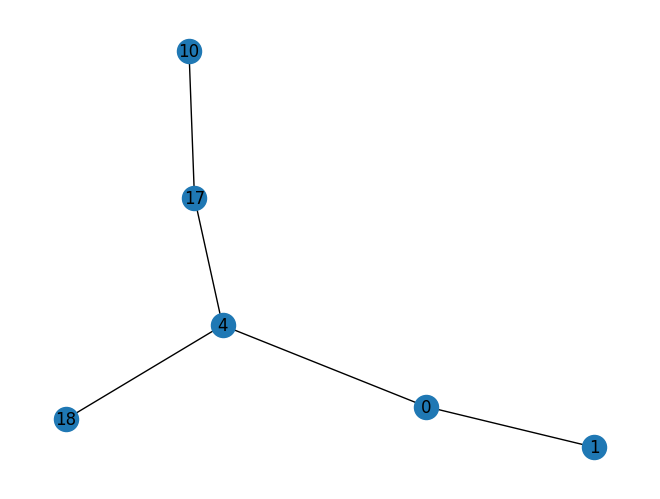
\includegraphics{Closeness_Centrality_files/figure-pdf/cell-16-output-1.png}

}

\end{figure}

\begin{Shaded}
\begin{Highlighting}[]
\CommentTok{\# Menggabungkan data closeness dengan data isi berita}
\NormalTok{closeness\_centrality}\OperatorTok{=}\NormalTok{ clean.join(df\_closeness)}
\CommentTok{\# closeness\_centrality}
\end{Highlighting}
\end{Shaded}

\begin{Shaded}
\begin{Highlighting}[]
\CommentTok{\# menambahkan index untuk urutan kalimat pada berita sebelum disorting}
\NormalTok{closeness\_centrality[}\StringTok{\textquotesingle{}Kalimat ke\textquotesingle{}}\NormalTok{] }\OperatorTok{=}\NormalTok{ closeness\_centrality.reset\_index(drop}\OperatorTok{=}\VariableTok{True}\NormalTok{).index }\OperatorTok{+} \DecValTok{1}
\CommentTok{\# closeness\_centrality}
\end{Highlighting}
\end{Shaded}

\hypertarget{meringkas-kalimat}{%
\section{Meringkas Kalimat}\label{meringkas-kalimat}}

\begin{Shaded}
\begin{Highlighting}[]
\CommentTok{\# melakukan sorting berdasarkan nilai Closeness Centrality tertinggi}
\NormalTok{closeness\_centrality.sort\_values(}\StringTok{\textquotesingle{}Closeness Centrality\textquotesingle{}}\NormalTok{, ascending}\OperatorTok{=}\VariableTok{False}\NormalTok{, inplace}\OperatorTok{=}\VariableTok{True}\NormalTok{)}

\CommentTok{\# Menampilkan DataFrame yang telah diurutkan}
\CommentTok{\# closeness\_centrality}
\end{Highlighting}
\end{Shaded}

\begin{Shaded}
\begin{Highlighting}[]
\CommentTok{\# Mengambil 6 kalimat dengan nilai closeness centrality tertinggi}
\NormalTok{top\_sentences }\OperatorTok{=}\NormalTok{ closeness\_centrality.head(}\DecValTok{6}\NormalTok{)}
\NormalTok{top\_sentences}
\end{Highlighting}
\end{Shaded}

\begin{longtable}[]{@{}llll@{}}
\toprule\noalign{}
& kalimat & Closeness Centrality & Kalimat ke \\
\midrule\noalign{}
\endhead
\bottomrule\noalign{}
\endlastfoot
4 & Saya harus bertanggung jawab. & 0.714286 & 5 \\
0 & POJOKBACA.ID PelatihManchester United MU Eri... & 0.555556 & 1 \\
17 & Saya bertanggung jawab, tetapi saya melihatny... & 0.555556 & 18 \\
18 & Saya harus tetap bersatu dengan para pemain da... & 0.454545 &
19 \\
1 & MU baru saja menelan kekalahan 0 3 dari Newcas... & 0.384615 & 2 \\
10 & Anda harus melakukannya sebagai sebuah tim. & 0.384615 & 11 \\
\end{longtable}

\begin{Shaded}
\begin{Highlighting}[]
\CommentTok{\# mengurutkan kalimat setelah melakukan pemilihan 6 kalimat terpenting berdasarkan nomer urut kalimat sebelumnya}
\NormalTok{result }\OperatorTok{=}\NormalTok{ top\_sentences.groupby(}\StringTok{\textquotesingle{}Kalimat ke\textquotesingle{}}\NormalTok{)[}\StringTok{\textquotesingle{}kalimat\textquotesingle{}}\NormalTok{].}\BuiltInTok{apply}\NormalTok{(}\StringTok{\textquotesingle{} \textquotesingle{}}\NormalTok{.join).reset\_index()}

\CommentTok{\# Menggabungkan kalimat yang terpisah sebelumnya menjadi 1}
\NormalTok{text }\OperatorTok{=} \StringTok{\textquotesingle{} \textquotesingle{}}\NormalTok{.join(result[}\StringTok{\textquotesingle{}kalimat\textquotesingle{}}\NormalTok{])}
\NormalTok{text}
\end{Highlighting}
\end{Shaded}

\begin{verbatim}
' POJOKBACA.ID  PelatihManchester United MU Erik ten Hagmengatakan bertanggung jawab penuh atas dua kekalahan timnya dengan skor 0 3 di Old Trafford. MU baru saja menelan kekalahan 0 3 dari Newcastle United pada ajang Piala Liga di Old Trafford, Kamis WIB. Saya harus bertanggung jawab. Anda harus melakukannya sebagai sebuah tim.  Saya bertanggung jawab, tetapi saya melihatnya sebagai sebuah tantangan. Saya harus tetap bersatu dengan para pemain dan berjuang bersama,  lanjutnya.'
\end{verbatim}

\hypertarget{modelling}{%
\section{Modelling}\label{modelling}}

\begin{Shaded}
\begin{Highlighting}[]
\ImportTok{from}\NormalTok{ sklearn.model\_selection }\ImportTok{import}\NormalTok{ train\_test\_split}
\ImportTok{from}\NormalTok{ sklearn.metrics }\ImportTok{import}\NormalTok{ accuracy\_score}
\ImportTok{from}\NormalTok{ sklearn.naive\_bayes }\ImportTok{import}\NormalTok{ GaussianNB}
\ImportTok{from}\NormalTok{ sklearn.neighbors }\ImportTok{import}\NormalTok{ KNeighborsClassifier}
\ImportTok{from}\NormalTok{ sklearn }\ImportTok{import}\NormalTok{ tree}
\end{Highlighting}
\end{Shaded}

\begin{Shaded}
\begin{Highlighting}[]
\CommentTok{\# Menghitung TF{-}IDF}
\NormalTok{vec }\OperatorTok{=}\NormalTok{ TfidfVectorizer()}
\NormalTok{tfidf }\OperatorTok{=}\NormalTok{ vec.fit\_transform(data[}\StringTok{\textquotesingle{}Isi\textquotesingle{}}\NormalTok{]).toarray()}
\end{Highlighting}
\end{Shaded}

\begin{Shaded}
\begin{Highlighting}[]
\NormalTok{y}\OperatorTok{=}\NormalTok{data[}\StringTok{\textquotesingle{}Kategori\textquotesingle{}}\NormalTok{]}
\NormalTok{X\_train,X\_test,y\_train,y\_test }\OperatorTok{=}\NormalTok{ train\_test\_split(tfidf,y,test\_size}\OperatorTok{=}\FloatTok{0.2}\NormalTok{,random\_state}\OperatorTok{=}\DecValTok{42}\NormalTok{)}
\end{Highlighting}
\end{Shaded}

\begin{Shaded}
\begin{Highlighting}[]
\NormalTok{NB }\OperatorTok{=}\NormalTok{ GaussianNB()}
\NormalTok{gaus}\OperatorTok{=}\NormalTok{NB.fit(X\_train, y\_train)}
\end{Highlighting}
\end{Shaded}

\begin{Shaded}
\begin{Highlighting}[]
\NormalTok{y\_pred }\OperatorTok{=}\NormalTok{ gaus.predict(X\_test)}
\NormalTok{accuracy }\OperatorTok{=}\NormalTok{ accuracy\_score(y\_test, y\_pred)}
\BuiltInTok{print}\NormalTok{(}\SpecialStringTok{f\textquotesingle{}Akurasi: }\SpecialCharTok{\{}\NormalTok{accuracy}\SpecialCharTok{\}}\SpecialStringTok{\textquotesingle{}}\NormalTok{)}
\end{Highlighting}
\end{Shaded}

\begin{verbatim}
Akurasi: 0.9204545454545454
\end{verbatim}

\begin{Shaded}
\begin{Highlighting}[]
\NormalTok{metode\_KNN }\OperatorTok{=}\NormalTok{ KNeighborsClassifier(n\_neighbors}\OperatorTok{=}\DecValTok{5}\NormalTok{)}
\NormalTok{metode\_KNN.fit(X\_train, y\_train)}
\end{Highlighting}
\end{Shaded}

\begin{verbatim}
KNeighborsClassifier()
\end{verbatim}

\begin{Shaded}
\begin{Highlighting}[]
\BuiltInTok{print}\NormalTok{(}\StringTok{"Hasil Akurasi Data Training Menggunakan KNN sebesar : "}\NormalTok{, (}\DecValTok{100} \OperatorTok{*}\NormalTok{ metode\_KNN.score(X\_train, y\_train)))}
\BuiltInTok{print}\NormalTok{(}\StringTok{"Hasil Akurasi Data Testing Menggunakan KNN sebesar : "}\NormalTok{, (}\DecValTok{100} \OperatorTok{*}\NormalTok{ (metode\_KNN.score(X\_test, y\_test))))}
\end{Highlighting}
\end{Shaded}

\begin{verbatim}
Hasil Akurasi Data Training Menggunakan KNN sebesar :  96.83908045977012
Hasil Akurasi Data Testing Menggunakan KNN sebesar :  98.86363636363636
\end{verbatim}

\begin{Shaded}
\begin{Highlighting}[]
\NormalTok{metode\_DT }\OperatorTok{=}\NormalTok{ tree.DecisionTreeClassifier(criterion}\OperatorTok{=}\StringTok{"gini"}\NormalTok{)}
\NormalTok{metode\_DT.fit(X\_train, y\_train)}
\end{Highlighting}
\end{Shaded}

\begin{verbatim}
DecisionTreeClassifier()
\end{verbatim}

\begin{Shaded}
\begin{Highlighting}[]
\BuiltInTok{print}\NormalTok{(}\StringTok{"Hasil Akurasi Data Training Menggunakan Decision Tree sebesar : "}\NormalTok{, (}\DecValTok{100} \OperatorTok{*}\NormalTok{ metode\_DT.score(X\_train, y\_train)))}
\BuiltInTok{print}\NormalTok{(}\StringTok{"Hasil Akurasi Data Testing Menggunakan Decision Tree sebesar : "}\NormalTok{, (}\DecValTok{100} \OperatorTok{*}\NormalTok{ (metode\_DT.score(X\_train, y\_train))))}
\end{Highlighting}
\end{Shaded}

\begin{verbatim}
Hasil Akurasi Data Training Menggunakan Decision Tree sebesar :  100.0
Hasil Akurasi Data Testing Menggunakan Decision Tree sebesar :  100.0
\end{verbatim}

\hypertarget{penerapan-pada-semua-berita-untuk-meringkas-semua-berita-nantinya}{%
\section{Penerapan pada semua berita untuk meringkas semua berita
nantinya}\label{penerapan-pada-semua-berita-untuk-meringkas-semua-berita-nantinya}}

\hypertarget{tokenisasi-per-kalimat}{%
\section{Tokenisasi per Kalimat}\label{tokenisasi-per-kalimat}}

\begin{Shaded}
\begin{Highlighting}[]
\CommentTok{\# membuat list untuk hasil tokenize}
\NormalTok{hasil\_kalimat}\OperatorTok{=}\NormalTok{[]}
\CommentTok{\# Melakukan perulangan untuk memisahkan berita per{-}kalimat}
\ControlFlowTok{for}\NormalTok{ i }\KeywordTok{in} \BuiltInTok{range}\NormalTok{(}\BuiltInTok{len}\NormalTok{(data)):}
\NormalTok{  token }\OperatorTok{=}\NormalTok{ sent\_tokenize(data[}\StringTok{\textquotesingle{}Isi\textquotesingle{}}\NormalTok{][i])}
\NormalTok{  hasil\_kalimat.append(token)}
\end{Highlighting}
\end{Shaded}

\begin{Shaded}
\begin{Highlighting}[]
\CommentTok{\# membuat list untuk hasil transpose tokenize sebelumnya}
\NormalTok{kalimat }\OperatorTok{=}\NormalTok{ []}
\CommentTok{\# melakukan perulangan untuk merubah hasil tokenize / transpose data}
\ControlFlowTok{for}\NormalTok{ i }\KeywordTok{in} \BuiltInTok{range}\NormalTok{(}\BuiltInTok{len}\NormalTok{(hasil\_kalimat)):}
  \ControlFlowTok{for}\NormalTok{ x }\KeywordTok{in} \BuiltInTok{range}\NormalTok{ (}\BuiltInTok{len}\NormalTok{(hasil\_kalimat[i])):}
\NormalTok{    datacek }\OperatorTok{=}\NormalTok{ []}
\NormalTok{    datacek.append(i)}
\NormalTok{    datacek.append(hasil\_kalimat[i][x])}
\NormalTok{    kalimat.append(datacek)}
\end{Highlighting}
\end{Shaded}

\begin{Shaded}
\begin{Highlighting}[]
\CommentTok{\# merubah hasil tokenize sebelumnya menjadi sebuah dataframe}
\NormalTok{databaru }\OperatorTok{=}\NormalTok{ pd.DataFrame(kalimat, columns}\OperatorTok{=}\NormalTok{[}\StringTok{"Dokumen ke"}\NormalTok{, }\StringTok{"Kalimat"}\NormalTok{])}
\NormalTok{databaru}
\end{Highlighting}
\end{Shaded}

\begin{longtable}[]{@{}lll@{}}
\toprule\noalign{}
& Dokumen ke & Kalimat \\
\midrule\noalign{}
\endhead
\bottomrule\noalign{}
\endlastfoot
0 & 0 & POJOKBACA.ID -PelatihManchester United(MU)Eri... \\
1 & 0 & MU baru saja menelan kekalahan 0-3 dari Newcas... \\
2 & 0 & Melalui gol dari Miguel Almiron, Lewis Hall, d... \\
3 & 0 & ``Ya, kami tahu ini tidak cukup baik. \\
4 & 0 & Saya harus bertanggung jawab. \\
... & ... & ... \\
7459 & 435 & Ini akan membantu memperpanjang umur bateraihp... \\
7460 & 435 & Itulah beberapa tips agarhptidak cepatlowbet. \\
7461 & 435 & Dengan mengikuti tips-tips di atas, pengguna d... \\
7462 & 435 & Selalu ingat untuk selalu membawa charger atau... \\
7463 & 435 & *** \\
\end{longtable}

\hypertarget{cleansing-1}{%
\section{Cleansing}\label{cleansing-1}}

\begin{Shaded}
\begin{Highlighting}[]
\CommentTok{\#Remove Puncutuation}
\NormalTok{clean\_symbol }\OperatorTok{=}\NormalTok{ re.}\BuiltInTok{compile}\NormalTok{(}\StringTok{\textquotesingle{}[\^{}\textbackslash{}w\textbackslash{}s.?!,/]\textquotesingle{}}\NormalTok{)}
\KeywordTok{def}\NormalTok{ clean\_punct(text):}
\NormalTok{    text }\OperatorTok{=}\NormalTok{ clean\_symbol.sub(}\StringTok{\textquotesingle{} \textquotesingle{}}\NormalTok{, text)}
    \ControlFlowTok{return}\NormalTok{ text}
\CommentTok{\# Buat kolom tambahan untuk data description yang telah diremovepunctuation}
\NormalTok{preprocessing }\OperatorTok{=}\NormalTok{ databaru[}\StringTok{\textquotesingle{}Kalimat\textquotesingle{}}\NormalTok{].}\BuiltInTok{apply}\NormalTok{(clean\_punct)}
\NormalTok{clean}\OperatorTok{=}\NormalTok{pd.DataFrame(preprocessing)}
\NormalTok{clean[}\StringTok{\textquotesingle{}Dokumen ke\textquotesingle{}}\NormalTok{]}\OperatorTok{=}\NormalTok{databaru[}\StringTok{\textquotesingle{}Dokumen ke\textquotesingle{}}\NormalTok{].values}
\NormalTok{clean}
\end{Highlighting}
\end{Shaded}

\begin{longtable}[]{@{}lll@{}}
\toprule\noalign{}
& Kalimat & Dokumen ke \\
\midrule\noalign{}
\endhead
\bottomrule\noalign{}
\endlastfoot
0 & POJOKBACA.ID PelatihManchester United MU Eri... & 0 \\
1 & MU baru saja menelan kekalahan 0 3 dari Newcas... & 0 \\
2 & Melalui gol dari Miguel Almiron, Lewis Hall, d... & 0 \\
3 & Ya, kami tahu ini tidak cukup baik. & 0 \\
4 & Saya harus bertanggung jawab. & 0 \\
... & ... & ... \\
7459 & Ini akan membantu memperpanjang umur bateraihp... & 435 \\
7460 & Itulah beberapa tips agarhptidak cepatlowbet. & 435 \\
7461 & Dengan mengikuti tips tips di atas, pengguna d... & 435 \\
7462 & Selalu ingat untuk selalu membawa charger atau... & 435 \\
7463 & & 435 \\
\end{longtable}

\hypertarget{tf-idf-1}{%
\section{TF-IDF}\label{tf-idf-1}}

\begin{Shaded}
\begin{Highlighting}[]
\CommentTok{\# Menghitung TF{-}IDF}
\NormalTok{vectorizer }\OperatorTok{=}\NormalTok{ TfidfVectorizer()}
\NormalTok{tfidf\_matrix }\OperatorTok{=}\NormalTok{ vectorizer.fit\_transform(clean[}\StringTok{\textquotesingle{}Kalimat\textquotesingle{}}\NormalTok{])}
\end{Highlighting}
\end{Shaded}

\begin{Shaded}
\begin{Highlighting}[]
\NormalTok{tf\_name}\OperatorTok{=}\NormalTok{vectorizer.get\_feature\_names\_out()}
\NormalTok{tf\_array }\OperatorTok{=}\NormalTok{ tfidf\_matrix.toarray()}

\NormalTok{df\_tf}\OperatorTok{=}\NormalTok{ pd.DataFrame(tf\_array, columns }\OperatorTok{=}\NormalTok{ tf\_name)}
\NormalTok{df\_tf}
\end{Highlighting}
\end{Shaded}

\begin{longtable}[]{@{}llllllllllllllllllllll@{}}
\toprule\noalign{}
& 00 & 000 & 000an & 000komputerdi & 000layar & 000samsung & 000x3 &
00151 & 004 & 01 & ... & zona & zondalam & zonjuga & zonmemastikan &
zontelah & zoom & zsemakin & zulhas & zulkifli & zurich \\
\midrule\noalign{}
\endhead
\bottomrule\noalign{}
\endlastfoot
0 & 0.0 & 0.0 & 0.0 & 0.0 & 0.0 & 0.0 & 0.0 & 0.0 & 0.0 & 0.0 & ... &
0.0 & 0.0 & 0.0 & 0.0 & 0.0 & 0.0 & 0.0 & 0.0 & 0.0 & 0.0 \\
1 & 0.0 & 0.0 & 0.0 & 0.0 & 0.0 & 0.0 & 0.0 & 0.0 & 0.0 & 0.0 & ... &
0.0 & 0.0 & 0.0 & 0.0 & 0.0 & 0.0 & 0.0 & 0.0 & 0.0 & 0.0 \\
2 & 0.0 & 0.0 & 0.0 & 0.0 & 0.0 & 0.0 & 0.0 & 0.0 & 0.0 & 0.0 & ... &
0.0 & 0.0 & 0.0 & 0.0 & 0.0 & 0.0 & 0.0 & 0.0 & 0.0 & 0.0 \\
3 & 0.0 & 0.0 & 0.0 & 0.0 & 0.0 & 0.0 & 0.0 & 0.0 & 0.0 & 0.0 & ... &
0.0 & 0.0 & 0.0 & 0.0 & 0.0 & 0.0 & 0.0 & 0.0 & 0.0 & 0.0 \\
4 & 0.0 & 0.0 & 0.0 & 0.0 & 0.0 & 0.0 & 0.0 & 0.0 & 0.0 & 0.0 & ... &
0.0 & 0.0 & 0.0 & 0.0 & 0.0 & 0.0 & 0.0 & 0.0 & 0.0 & 0.0 \\
... & ... & ... & ... & ... & ... & ... & ... & ... & ... & ... & ... &
... & ... & ... & ... & ... & ... & ... & ... & ... & ... \\
7459 & 0.0 & 0.0 & 0.0 & 0.0 & 0.0 & 0.0 & 0.0 & 0.0 & 0.0 & 0.0 & ... &
0.0 & 0.0 & 0.0 & 0.0 & 0.0 & 0.0 & 0.0 & 0.0 & 0.0 & 0.0 \\
7460 & 0.0 & 0.0 & 0.0 & 0.0 & 0.0 & 0.0 & 0.0 & 0.0 & 0.0 & 0.0 & ... &
0.0 & 0.0 & 0.0 & 0.0 & 0.0 & 0.0 & 0.0 & 0.0 & 0.0 & 0.0 \\
7461 & 0.0 & 0.0 & 0.0 & 0.0 & 0.0 & 0.0 & 0.0 & 0.0 & 0.0 & 0.0 & ... &
0.0 & 0.0 & 0.0 & 0.0 & 0.0 & 0.0 & 0.0 & 0.0 & 0.0 & 0.0 \\
7462 & 0.0 & 0.0 & 0.0 & 0.0 & 0.0 & 0.0 & 0.0 & 0.0 & 0.0 & 0.0 & ... &
0.0 & 0.0 & 0.0 & 0.0 & 0.0 & 0.0 & 0.0 & 0.0 & 0.0 & 0.0 \\
7463 & 0.0 & 0.0 & 0.0 & 0.0 & 0.0 & 0.0 & 0.0 & 0.0 & 0.0 & 0.0 & ... &
0.0 & 0.0 & 0.0 & 0.0 & 0.0 & 0.0 & 0.0 & 0.0 & 0.0 & 0.0 \\
\end{longtable}

\hypertarget{cosine-similarity-1}{%
\section{Cosine Similarity}\label{cosine-similarity-1}}

\begin{Shaded}
\begin{Highlighting}[]
\CommentTok{\# Menghitung cosine similarity}
\NormalTok{cosine\_similarities }\OperatorTok{=}\NormalTok{ cosine\_similarity(tfidf\_matrix, tfidf\_matrix)}
\end{Highlighting}
\end{Shaded}

\begin{Shaded}
\begin{Highlighting}[]
\CommentTok{\# menyetel batas threshold untuk closeness centrality sebesar 0,5}
\NormalTok{threshold}\OperatorTok{=}\FloatTok{0.5}
\CommentTok{\# inisiasi variabel G sebagai graph}
\NormalTok{G }\OperatorTok{=}\NormalTok{ nx.Graph()}
\CommentTok{\# perulangan untuk menghitung closeness centrality antar dokumen berdasarkan jumlah cosine similarities}
\ControlFlowTok{for}\NormalTok{ i }\KeywordTok{in} \BuiltInTok{range}\NormalTok{(}\BuiltInTok{len}\NormalTok{(cosine\_similarities)):}
    \ControlFlowTok{for}\NormalTok{ j }\KeywordTok{in} \BuiltInTok{range}\NormalTok{(}\BuiltInTok{len}\NormalTok{(cosine\_similarities)):}
      \CommentTok{\# melakukan permisalan agar kalimat tidak dibandindkan dengan kalimat yang sama}
      \ControlFlowTok{if}\NormalTok{ i }\OperatorTok{!=}\NormalTok{ j:}
\NormalTok{        sim }\OperatorTok{=}\NormalTok{ cosine\_similarities[i][j]}
        \CommentTok{\# melakukan pembatasan sehingga yang diinputkan hanya yang diatas nilai threshold}
        \ControlFlowTok{if}\NormalTok{ sim }\OperatorTok{\textgreater{}}\NormalTok{ threshold:}
\NormalTok{          G.add\_edge(i, j, weight}\OperatorTok{=}\NormalTok{sim)}
          \BuiltInTok{print}\NormalTok{(i,}\StringTok{\textquotesingle{},\textquotesingle{}}\NormalTok{,j,}\StringTok{\textquotesingle{}=\textquotesingle{}}\NormalTok{,sim)}
\end{Highlighting}
\end{Shaded}

\begin{verbatim}
4 , 17 = 0.6233405154424684
17 , 4 = 0.6233405154424684
22 , 1490 = 0.532261281228443
23 , 5825 = 0.513426149077395
25 , 1497 = 0.6300592020286585
25 , 2954 = 0.5489844080764691
26 , 765 = 0.5359105829313249
27 , 1113 = 0.7610483305323376
27 , 1497 = 0.6629885321504021
27 , 2747 = 0.5442699431289661
27 , 3098 = 0.5359129829436925
27 , 5014 = 0.7032926366111086
27 , 5577 = 0.8550864121555564
27 , 5885 = 0.6572431643869489
27 , 6381 = 0.5651739149410978
28 , 1114 = 0.6854371156816045
28 , 1498 = 0.6854371156816045
28 , 3099 = 0.6854371156816045
28 , 3205 = 0.5402467666605076
28 , 3317 = 0.6854371156816045
28 , 3874 = 0.6854371156816045
28 , 4478 = 0.662297128875452
28 , 5015 = 0.5421001888881218
28 , 5578 = 0.6165679430530828
28 , 5886 = 0.6854371156816045
29 , 3101 = 0.9669289131356907
29 , 4479 = 0.9743256923317468
29 , 5016 = 0.9743256923317468
29 , 5579 = 1.0
29 , 7419 = 0.881747018473719
30 , 2048 = 0.8526487082945213
30 , 2766 = 0.5775875829579953
30 , 5146 = 0.5116548099269025
52 , 65 = 0.5456678380229698
62 , 573 = 0.8122753003753505
62 , 1515 = 0.6956142253364047
62 , 3103 = 0.7347972441145723
62 , 4480 = 0.7298114528193883
62 , 4575 = 0.7133998940455695
62 , 5017 = 0.7311506506082271
62 , 5384 = 0.5821680652183471
62 , 6463 = 0.855522260311586
63 , 6464 = 0.5532693051898747
64 , 574 = 0.5707781754137486
65 , 52 = 0.5456678380229698
66 , 4037 = 0.5919675920072446
67 , 4422 = 0.5087691538764314
74 , 76 = 0.5339881002564392
76 , 74 = 0.5339881002564392
99 , 1072 = 0.6492341216387344
99 , 6322 = 0.5707897607704538
109 , 5887 = 1.0
110 , 5888 = 1.0000000000000002
111 , 5889 = 1.0
112 , 5890 = 1.0000000000000002
113 , 2597 = 0.5892034886609564
114 , 2537 = 0.9302720805968582
114 , 2562 = 0.5307242122023833
114 , 5893 = 1.0
115 , 5894 = 1.0
116 , 5895 = 1.0
117 , 5896 = 0.7496171410645703
118 , 5897 = 1.0
119 , 5898 = 1.0000000000000002
120 , 5899 = 1.0000000000000002
121 , 5900 = 0.6956664053601072
134 , 4996 = 0.5039861632059406
138 , 7171 = 0.5439627878505164
180 , 5598 = 0.6162133399472685
180 , 6459 = 1.0000000000000002
182 , 4043 = 0.6816239457485662
183 , 4045 = 0.7959506911780974
185 , 4047 = 0.8459366284863548
186 , 1996 = 0.5553941582325926
187 , 2814 = 1.0
189 , 5793 = 0.7910161618486473
189 , 6503 = 0.504215458558591
189 , 6708 = 0.7910161618486473
193 , 2832 = 0.513342839847862
201 , 4949 = 0.7206643817285072
201 , 5232 = 0.6945634373164156
204 , 4952 = 1.0000000000000002
205 , 4953 = 1.0000000000000002
205 , 5235 = 1.0000000000000002
212 , 4957 = 1.0000000000000002
212 , 5238 = 1.0000000000000002
215 , 458 = 0.6029153729100647
215 , 5122 = 0.556267340909934
218 , 461 = 0.639475726467611
218 , 5124 = 1.0
219 , 462 = 0.8940925678511
219 , 5125 = 0.8697805981682607
223 , 466 = 0.8221882311938976
223 , 5131 = 0.8220123060003588
224 , 467 = 1.0000000000000002
224 , 5129 = 0.5602458356379416
224 , 5132 = 1.0000000000000002
225 , 468 = 0.6766052069756658
225 , 5133 = 0.76657125536237
243 , 252 = 0.6606957590657165
243 , 1082 = 0.5124695114758329
243 , 1749 = 0.6749667201404144
245 , 1270 = 0.5068302695239256
248 , 2038 = 0.620008056890546
248 , 3358 = 0.8825936692304511
252 , 243 = 0.6606957590657165
257 , 2041 = 1.0
292 , 3165 = 0.5173320189440614
300 , 2748 = 0.6827050843413364
304 , 2754 = 0.8293219798828643
305 , 2755 = 0.7415020748853434
308 , 2757 = 0.631311144624934
311 , 2759 = 1.0000000000000002
312 , 2760 = 1.0
321 , 3147 = 1.0000000000000002
321 , 5275 = 0.6064080523428002
322 , 4017 = 0.5651140835701789
322 , 6191 = 0.9273347248889794
328 , 492 = 0.5727441300851779
335 , 4978 = 0.6627962383660169
336 , 4979 = 0.6325325515090914
355 , 6224 = 0.5910260582736827
391 , 392 = 0.6205801237883442
392 , 391 = 0.6205801237883442
408 , 6065 = 0.5246601825110084
412 , 431 = 0.5468453885962631
431 , 412 = 0.5468453885962631
439 , 2084 = 0.6517403970746249
439 , 2674 = 0.5761191480650651
451 , 4434 = 0.620161488667882
452 , 454 = 0.6062720898692622
454 , 452 = 0.6062720898692622
458 , 215 = 0.6029153729100647
458 , 5122 = 0.6494363397293146
461 , 218 = 0.639475726467611
461 , 5124 = 0.639475726467611
462 , 219 = 0.8940925678511
462 , 5125 = 0.8498007206212244
463 , 1513 = 1.0
464 , 1514 = 1.0
466 , 223 = 0.8221882311938976
466 , 5131 = 0.7528921912933054
467 , 224 = 1.0000000000000002
467 , 5129 = 0.5602458356379416
467 , 5132 = 1.0000000000000002
468 , 225 = 0.6766052069756658
468 , 5133 = 0.6229359201094349
472 , 473 = 0.5748838131607231
472 , 474 = 0.6386423806789995
472 , 475 = 0.6392507746591533
472 , 5137 = 1.0000000000000002
472 , 5138 = 0.5748838131607231
472 , 5139 = 0.6386423806789995
472 , 5140 = 0.606542080171044
473 , 472 = 0.5748838131607231
473 , 474 = 0.7498592414926293
473 , 475 = 0.7505735847029901
473 , 476 = 0.5531510463712817
473 , 477 = 0.6802547094465833
473 , 5137 = 0.5748838131607231
473 , 5138 = 1.0
473 , 5139 = 0.7498592414926293
473 , 5140 = 0.7121688098538941
473 , 5141 = 0.5531510463712817
473 , 5142 = 0.6802547094465833
474 , 472 = 0.6386423806789995
474 , 473 = 0.7498592414926293
474 , 475 = 0.9102330682203454
474 , 477 = 0.6249663096265637
474 , 5137 = 0.6386423806789995
474 , 5138 = 0.7498592414926293
474 , 5139 = 1.0000000000000002
474 , 5140 = 0.8636589590888107
474 , 5142 = 0.6249663096265637
475 , 472 = 0.6392507746591533
475 , 473 = 0.7505735847029901
475 , 474 = 0.9102330682203454
475 , 477 = 0.6255616752835869
475 , 5137 = 0.6392507746591533
475 , 5138 = 0.7505735847029901
475 , 5139 = 0.9102330682203454
475 , 5140 = 0.8644817120527729
475 , 5142 = 0.6255616752835869
476 , 473 = 0.5531510463712817
476 , 477 = 0.5218166715566447
476 , 5138 = 0.5531510463712817
476 , 5141 = 1.0
476 , 5142 = 0.5218166715566447
477 , 473 = 0.6802547094465833
477 , 474 = 0.6249663096265637
477 , 475 = 0.6255616752835869
477 , 476 = 0.5218166715566447
477 , 478 = 0.561558802359594
477 , 5138 = 0.6802547094465833
477 , 5139 = 0.6249663096265637
477 , 5140 = 0.5935534141575358
477 , 5141 = 0.5218166715566447
477 , 5142 = 1.0
477 , 5143 = 0.561558802359594
478 , 477 = 0.561558802359594
478 , 5142 = 0.561558802359594
478 , 5143 = 1.0000000000000002
481 , 1930 = 0.7059726281826335
481 , 5145 = 0.5670454913466347
482 , 1931 = 1.0000000000000002
483 , 1932 = 0.8881814068577042
485 , 486 = 0.5153712882727686
486 , 485 = 0.5153712882727686
492 , 328 = 0.5727441300851779
498 , 1119 = 0.5935211528185876
500 , 5691 = 0.5743025728577508
500 , 6304 = 0.5743025728577508
501 , 514 = 0.6008080758856248
514 , 501 = 0.6008080758856248
519 , 3588 = 0.5630665725028321
519 , 6358 = 0.5668247330823871
538 , 7434 = 0.5220505381290343
541 , 922 = 0.5442755656556406
541 , 6061 = 0.542427059510457
541 , 7435 = 0.8049211824723789
542 , 7438 = 0.5307270023770811
545 , 2753 = 1.0000000000000002
548 , 2538 = 0.5360703964915412
549 , 2802 = 0.5808956346933011
562 , 563 = 0.6678467826712874
563 , 562 = 0.6678467826712874
567 , 6455 = 0.5433721421214842
570 , 2199 = 0.5298928856668578
573 , 62 = 0.8122753003753505
573 , 1515 = 0.5985588603810028
573 , 3103 = 0.6681556805745924
573 , 4480 = 0.6425546967836986
573 , 4575 = 0.6484150742494049
573 , 5017 = 0.6437337791697266
573 , 5384 = 0.501739290747991
573 , 6463 = 0.76421662207179
574 , 64 = 0.5707781754137486
578 , 2240 = 0.5359418508458835
578 , 3307 = 0.5134912278847128
581 , 3311 = 1.0
603 , 3948 = 1.0
672 , 7325 = 0.5039109494656526
685 , 1282 = 0.5241950111504401
694 , 695 = 0.6042080054021388
695 , 694 = 0.6042080054021388
697 , 698 = 0.824198032020534
698 , 697 = 0.824198032020534
717 , 718 = 0.6324283871814428
718 , 717 = 0.6324283871814428
730 , 732 = 0.5087117575698654
732 , 730 = 0.5087117575698654
733 , 4268 = 1.0
733 , 5423 = 0.5833868741274642
743 , 951 = 0.5171732688153605
764 , 1877 = 0.6247450449259886
764 , 6919 = 0.6247450449259886
765 , 26 = 0.5359105829313249
766 , 6921 = 0.5124072316553335
767 , 3073 = 0.5323020169864342
770 , 3069 = 1.0000000000000002
771 , 3070 = 0.8721093093929441
771 , 5748 = 0.5962991583037492
772 , 3071 = 0.941912007615337
773 , 3072 = 0.854141107101451
774 , 3074 = 1.0000000000000002
775 , 3075 = 0.9695400725679885
776 , 3076 = 1.0000000000000002
777 , 3077 = 1.0000000000000002
778 , 3078 = 1.0000000000000002
794 , 5568 = 0.5241004653269233
800 , 3001 = 0.5725862748970776
806 , 808 = 0.7225051057557546
808 , 806 = 0.7225051057557546
813 , 857 = 0.8205198467537754
814 , 858 = 0.7014038918337444
815 , 859 = 1.0000000000000002
815 , 2193 = 0.5338608230807205
816 , 860 = 0.520913828031635
816 , 861 = 0.5203143554706914
818 , 863 = 0.6306929958952563
838 , 3401 = 0.5791249587350563
846 , 6831 = 0.5188561702878901
855 , 4211 = 0.6471641093874233
856 , 4212 = 0.9706860727257012
857 , 813 = 0.8205198467537754
858 , 814 = 0.7014038918337444
859 , 815 = 1.0000000000000002
859 , 2193 = 0.5338608230807205
860 , 816 = 0.520913828031635
861 , 816 = 0.5203143554706914
863 , 818 = 0.6306929958952563
878 , 6329 = 0.7229202063003566
879 , 6330 = 0.9492901985406336
884 , 6335 = 0.5366008801673038
885 , 6172 = 0.5399354975057904
885 , 6337 = 0.5961825516326508
886 , 6173 = 0.7560664144716986
892 , 6860 = 1.0
893 , 3200 = 0.6568138595143661
905 , 2064 = 0.5462382011179555
905 , 4434 = 0.5046238078504129
905 , 5958 = 0.5328304677747996
913 , 917 = 0.5090332474691929
913 , 4430 = 0.5248553567593547
913 , 4436 = 0.6353827579855612
915 , 4435 = 0.6078917888975608
917 , 913 = 0.5090332474691929
921 , 3985 = 0.5482396248001553
922 , 541 = 0.5442755656556406
923 , 1718 = 0.5058398598306035
923 , 5703 = 0.5766981951514718
923 , 7438 = 0.5628040184467541
950 , 1368 = 0.538777503071977
950 , 4022 = 0.6290404113518702
951 , 743 = 0.5171732688153605
953 , 965 = 0.5045497961318993
961 , 1379 = 0.5597871028716191
965 , 953 = 0.5045497961318993
967 , 1369 = 0.6148256843721553
992 , 6430 = 1.0000000000000002
995 , 6901 = 0.9258649322393475
996 , 1000 = 0.526314187638504
1000 , 996 = 0.526314187638504
1003 , 4158 = 0.5765547931435995
1007 , 4159 = 1.0000000000000002
1033 , 1034 = 0.670044238304264
1034 , 1033 = 0.670044238304264
1037 , 2727 = 0.5148948304307737
1062 , 6309 = 0.5365056954546226
1065 , 6311 = 0.8377343971379857
1066 , 6312 = 0.6447925660677636
1069 , 6316 = 0.8510671557286611
1070 , 6320 = 1.0
1071 , 6321 = 1.0000000000000002
1072 , 99 = 0.6492341216387344
1072 , 4529 = 0.567144536110197
1072 , 6322 = 0.5963851126197685
1074 , 5943 = 0.5016621412932567
1075 , 1803 = 0.5021343349663437
1075 , 5940 = 0.5889495721461734
1075 , 6545 = 0.518190053274893
1082 , 243 = 0.5124695114758329
1107 , 6839 = 0.5669738391056087
1112 , 5751 = 1.0
1112 , 6844 = 1.0
1113 , 27 = 0.7610483305323376
1113 , 1497 = 0.5941665210395866
1113 , 2747 = 0.5020531156313699
1113 , 3098 = 0.6232559039684851
1113 , 3316 = 0.5742421816469143
1113 , 5014 = 0.5075617987916371
1113 , 5577 = 0.6537005640643319
1113 , 5885 = 0.6063165427298022
1113 , 6381 = 0.691202195227087
1113 , 6931 = 0.5957791256977043
1114 , 28 = 0.6854371156816045
1114 , 1498 = 1.0000000000000002
1114 , 3099 = 1.0000000000000002
1114 , 3317 = 1.0000000000000002
1114 , 3874 = 1.0000000000000002
1114 , 4478 = 0.9656331393672325
1114 , 5015 = 0.6291492382570958
1114 , 5578 = 0.7227778244726916
1114 , 5886 = 1.0000000000000002
1118 , 1120 = 0.623576388802527
1119 , 498 = 0.5935211528185876
1120 , 1118 = 0.623576388802527
1123 , 1126 = 0.6350966708420799
1126 , 1123 = 0.6350966708420799
1187 , 1197 = 0.582163311762683
1191 , 1208 = 0.5446581908115629
1197 , 1187 = 0.582163311762683
1208 , 1191 = 0.5446581908115629
1255 , 5906 = 0.5198012070127843
1257 , 2592 = 0.5703562653653756
1270 , 245 = 0.5068302695239256
1270 , 3355 = 0.5145745418284401
1273 , 5189 = 0.5269220491243083
1274 , 4614 = 0.5354599677138081
1276 , 5191 = 0.5921958020644109
1278 , 5192 = 0.5860546593202074
1279 , 5385 = 0.5334071166593158
1280 , 5386 = 0.5087968367689809
1282 , 685 = 0.5241950111504401
1284 , 5387 = 1.0000000000000002
1285 , 5388 = 0.8821018689681724
1287 , 5389 = 0.6332514528858755
1314 , 6297 = 0.7138131322519652
1345 , 7360 = 0.5384381269356258
1349 , 7366 = 0.5647903258882925
1361 , 3469 = 0.6630434676369622
1368 , 950 = 0.538777503071977
1369 , 967 = 0.6148256843721553
1376 , 1378 = 0.5101104300135819
1378 , 1376 = 0.5101104300135819
1379 , 961 = 0.5597871028716191
1385 , 1401 = 0.9870009292547848
1386 , 1402 = 1.0
1387 , 1403 = 1.0000000000000002
1388 , 1404 = 0.9999999999999998
1389 , 1405 = 1.0
1391 , 1406 = 0.8649044169088631
1392 , 1407 = 1.0000000000000002
1393 , 1408 = 0.9999999999999997
1396 , 4350 = 0.6278826299050829
1398 , 4488 = 0.5662944942536864
1401 , 1385 = 0.9870009292547848
1402 , 1386 = 1.0
1403 , 1387 = 1.0000000000000002
1404 , 1388 = 0.9999999999999998
1405 , 1389 = 1.0
1406 , 1391 = 0.8649044169088631
1407 , 1392 = 1.0000000000000002
1408 , 1393 = 0.9999999999999997
1435 , 4219 = 1.0
1439 , 4223 = 0.7143866043554462
1450 , 4228 = 0.6456229649464129
1451 , 4230 = 1.0000000000000004
1452 , 4231 = 0.7353785943004285
1469 , 6079 = 0.5750945923496824
1486 , 1496 = 0.6850648841969259
1490 , 22 = 0.532261281228443
1496 , 1486 = 0.6850648841969259
1497 , 25 = 0.6300592020286585
1497 , 27 = 0.6629885321504021
1497 , 1113 = 0.5941665210395866
1497 , 2747 = 0.5364090091122037
1497 , 2954 = 0.5046900463644675
1497 , 5014 = 0.5696420269218552
1497 , 5577 = 0.5984677697985101
1497 , 5885 = 0.649234113773599
1497 , 6381 = 0.5781073134654557
1497 , 6931 = 0.5016471576848442
1498 , 28 = 0.6854371156816045
1498 , 1114 = 1.0000000000000002
1498 , 3099 = 1.0000000000000002
1498 , 3317 = 1.0000000000000002
1498 , 3874 = 1.0000000000000002
1498 , 4478 = 0.9656331393672325
1498 , 5015 = 0.6291492382570958
1498 , 5578 = 0.7227778244726916
1498 , 5886 = 1.0000000000000002
1500 , 5684 = 0.5144438090148887
1513 , 463 = 1.0
1514 , 464 = 1.0
1515 , 62 = 0.6956142253364047
1515 , 573 = 0.5985588603810028
1515 , 3103 = 0.5371359392977009
1515 , 4480 = 0.546216516179887
1515 , 4575 = 0.8209639178483505
1515 , 5017 = 0.5472188188265082
1515 , 6463 = 0.5912229499086106
1515 , 6825 = 0.6061121758094226
1522 , 1539 = 0.5566685570939178
1525 , 1527 = 0.5108953720142034
1527 , 1525 = 0.5108953720142034
1537 , 1541 = 0.6098834805588534
1539 , 1522 = 0.5566685570939178
1541 , 1537 = 0.6098834805588534
1572 , 2794 = 0.5375461152582929
1572 , 3861 = 0.5699305771897419
1572 , 4350 = 0.5121360967495854
1572 , 6084 = 0.776906493518668
1572 , 7145 = 0.518545956380219
1614 , 1622 = 0.5615845486950273
1622 , 1614 = 0.5615845486950273
1622 , 1631 = 0.6098659462600032
1626 , 2867 = 0.6129230626527763
1631 , 1622 = 0.6098659462600032
1646 , 3330 = 0.5213779157885834
1676 , 5322 = 0.5174684859800228
1703 , 1706 = 0.6839033602304193
1706 , 1703 = 0.6839033602304193
1717 , 3401 = 0.5816957542672008
1717 , 6357 = 0.5673646283002329
1718 , 923 = 0.5058398598306035
1718 , 3588 = 0.5453485949594944
1718 , 5703 = 0.6724025313580582
1718 , 6358 = 0.7479358035413459
1720 , 3598 = 0.6584534437095705
1720 , 5026 = 0.6265544370903834
1721 , 5712 = 0.6177591262756654
1736 , 1739 = 0.6160374606978095
1739 , 1736 = 0.6160374606978095
1749 , 243 = 0.6749667201404144
1754 , 1766 = 0.5771791786022202
1756 , 3662 = 0.5409720080512841
1757 , 3663 = 1.0
1758 , 3664 = 0.8360682062804999
1759 , 3665 = 0.8323488849670945
1761 , 3667 = 0.9139025014479669
1762 , 3668 = 0.9096088990445624
1763 , 3669 = 0.9120744249271429
1764 , 3670 = 1.0000000000000002
1766 , 1754 = 0.5771791786022202
1788 , 7369 = 0.5957993048876911
1796 , 5910 = 0.6439678190820209
1803 , 1075 = 0.5021343349663437
1817 , 1823 = 0.5607394900692438
1823 , 1817 = 0.5607394900692438
1823 , 1825 = 0.5079721074080565
1825 , 1823 = 0.5079721074080565
1847 , 5071 = 0.9318861143092914
1854 , 5633 = 0.6052544749116772
1854 , 6023 = 0.6039769679811414
1854 , 7438 = 0.6339838980758913
1860 , 3991 = 0.5101086388417243
1861 , 3217 = 0.526891429232903
1870 , 1871 = 0.6422176779487888
1871 , 1870 = 0.6422176779487888
1876 , 6918 = 0.7975269942600562
1877 , 764 = 0.6247450449259886
1877 , 6919 = 1.0000000000000002
1878 , 6920 = 1.0
1879 , 6921 = 0.5074098349353177
1880 , 6922 = 1.0000000000000002
1881 , 6923 = 1.0000000000000002
1882 , 6924 = 0.6569123860829807
1883 , 1884 = 0.6744384019845342
1883 , 6925 = 1.0000000000000002
1883 , 6926 = 0.6744384019845342
1884 , 1883 = 0.6744384019845342
1884 , 6925 = 0.6744384019845342
1884 , 6926 = 1.0000000000000002
1885 , 6927 = 0.9262380721303545
1886 , 6928 = 0.6644770311635608
1887 , 6929 = 0.8313063382458978
1888 , 6930 = 1.0000000000000004
1900 , 6372 = 0.743448296348834
1930 , 481 = 0.7059726281826335
1931 , 482 = 1.0000000000000002
1932 , 483 = 0.8881814068577042
1948 , 4104 = 0.5401156399190981
1948 , 5593 = 0.5012906674826532
1961 , 7088 = 0.8388231578778673
1965 , 2727 = 0.5154932220445695
1976 , 1982 = 0.5827403275418945
1982 , 1976 = 0.5827403275418945
1985 , 3403 = 0.6773823168737133
1989 , 2290 = 1.0000000000000002
1996 , 186 = 0.5553941582325926
1997 , 2201 = 1.0
1997 , 4104 = 0.8343427845218032
1997 , 4801 = 0.9113783440899417
1997 , 6535 = 0.9502636491693826
2038 , 248 = 0.620008056890546
2038 , 3358 = 0.7024841424833038
2041 , 257 = 1.0
2044 , 2045 = 0.5257690199303928
2045 , 2044 = 0.5257690199303928
2048 , 30 = 0.8526487082945213
2048 , 2766 = 0.6107180303742046
2048 , 5146 = 0.639823998472809
2064 , 905 = 0.5462382011179555
2064 , 5958 = 0.5023297773836168
2069 , 2073 = 0.629878591875455
2073 , 2069 = 0.629878591875455
2084 , 439 = 0.6517403970746249
2084 , 2674 = 0.5055736077581402
2091 , 3526 = 0.677011621944097
2092 , 3527 = 0.8105040712414007
2093 , 3528 = 1.0000000000000002
2094 , 3529 = 0.7629470506155689
2095 , 3530 = 0.8516208960348948
2096 , 3531 = 0.8506301076912299
2098 , 3532 = 0.6525104578020804
2099 , 3533 = 0.8343565895315077
2123 , 3677 = 0.6291398930281844
2177 , 4765 = 0.503470842192755
2177 , 5215 = 0.6814823510202404
2188 , 5697 = 0.6672058736543965
2188 , 5699 = 1.0000000000000004
2188 , 6296 = 0.6805044447785523
2188 , 6297 = 0.7394358874175982
2191 , 4808 = 0.5290315206849157
2193 , 815 = 0.5338608230807205
2193 , 859 = 0.5338608230807205
2196 , 4811 = 0.6725234093765782
2199 , 570 = 0.5298928856668578
2201 , 1997 = 1.0
2201 , 4104 = 0.8343427845218032
2201 , 4801 = 0.9113783440899417
2201 , 6535 = 0.9502636491693826
2214 , 2223 = 0.5257290136855042
2214 , 2225 = 0.5350986240418115
2216 , 2227 = 0.9320856457302611
2217 , 2230 = 0.6014076302345744
2223 , 2214 = 0.5257290136855042
2225 , 2214 = 0.5350986240418115
2227 , 2216 = 0.9320856457302611
2230 , 2217 = 0.6014076302345744
2240 , 578 = 0.5359418508458835
2240 , 3307 = 0.625904399989425
2243 , 2538 = 0.53678954786491
2257 , 5731 = 0.5157065728916395
2290 , 1989 = 1.0000000000000002
2310 , 7401 = 0.5825647317436492
2315 , 2609 = 0.5812254923657414
2320 , 2612 = 0.6200621635122487
2320 , 5468 = 0.5439089111863568
2320 , 5495 = 0.6371469433658673
2321 , 7284 = 0.5213226368721302
2335 , 2337 = 0.5380638194118763
2337 , 2335 = 0.5380638194118763
2375 , 4504 = 0.5754627854569915
2422 , 4068 = 0.5330455286749669
2425 , 2426 = 0.5465161998188632
2426 , 2425 = 0.5465161998188632
2436 , 6835 = 0.5575399906684968
2479 , 2481 = 0.5228483864389102
2481 , 2479 = 0.5228483864389102
2481 , 3640 = 0.5254086837742005
2490 , 3252 = 0.5857797177342703
2500 , 2506 = 0.5643029473283376
2502 , 3210 = 0.5777216534520171
2506 , 2500 = 0.5643029473283376
2511 , 2513 = 0.5742507195853608
2513 , 2511 = 0.5742507195853608
2535 , 3203 = 0.6041688106577632
2537 , 114 = 0.9302720805968582
2537 , 2562 = 0.5420578852675639
2537 , 5893 = 0.9302720805968582
2538 , 548 = 0.5360703964915412
2538 , 2243 = 0.53678954786491
2538 , 2561 = 0.585839305341528
2542 , 6001 = 0.5158588992666273
2550 , 5461 = 1.0
2554 , 2948 = 0.6618191980807919
2561 , 2538 = 0.585839305341528
2562 , 114 = 0.5307242122023833
2562 , 2537 = 0.5420578852675639
2562 , 5893 = 0.5307242122023833
2592 , 1257 = 0.5703562653653756
2597 , 113 = 0.5892034886609564
2598 , 5469 = 0.5147617293799951
2599 , 4824 = 0.5327957612540627
2599 , 4826 = 0.6240147731937005
2600 , 4818 = 0.8518114891663139
2601 , 4820 = 0.9142118480549266
2602 , 4819 = 0.9266677761950203
2609 , 2315 = 0.5812254923657414
2612 , 2320 = 0.6200621635122487
2612 , 5468 = 0.589415404753581
2612 , 5495 = 0.634726187592492
2612 , 5634 = 0.5344558839292443
2615 , 2616 = 0.6803187369440703
2616 , 2615 = 0.6803187369440703
2639 , 7068 = 0.5708438553991513
2642 , 6386 = 0.5188760196136979
2642 , 7059 = 0.6237060758941193
2643 , 7062 = 0.6653162731721814
2656 , 6914 = 0.5243062455332884
2656 , 7369 = 0.5157032318522708
2667 , 3994 = 0.5190159267612496
2674 , 439 = 0.5761191480650651
2674 , 2084 = 0.5055736077581402
2683 , 6493 = 0.5295781391445992
2690 , 7079 = 0.5152882301536571
2693 , 5489 = 0.5604666286798272
2694 , 5491 = 0.943704127763333
2697 , 5481 = 0.6851805077150956
2698 , 5481 = 0.5687276298907754
2699 , 5482 = 0.6525103642832992
2725 , 4237 = 0.6927575327104902
2727 , 1037 = 0.5148948304307737
2727 , 1965 = 0.5154932220445695
2728 , 5022 = 0.5309612318074661
2731 , 3594 = 0.5013828108791004
2747 , 27 = 0.5442699431289661
2747 , 1113 = 0.5020531156313699
2747 , 1497 = 0.5364090091122037
2747 , 3098 = 0.5071033637020098
2747 , 5014 = 0.6203773847677595
2747 , 5577 = 0.6473651914744935
2747 , 5851 = 0.5924430054890738
2747 , 5875 = 0.5651579405488968
2747 , 5885 = 0.6915887672502018
2747 , 6381 = 0.629001593189228
2747 , 6931 = 0.5609194800905313
2748 , 300 = 0.6827050843413364
2753 , 545 = 1.0000000000000002
2754 , 304 = 0.8293219798828643
2755 , 305 = 0.7415020748853434
2757 , 308 = 0.631311144624934
2759 , 311 = 1.0000000000000002
2760 , 312 = 1.0
2761 , 2763 = 0.5558250970233026
2763 , 2761 = 0.5558250970233026
2766 , 30 = 0.5775875829579953
2766 , 2048 = 0.6107180303742046
2771 , 2785 = 0.7316021359495498
2771 , 4617 = 0.5979679308215157
2785 , 2771 = 0.7316021359495498
2793 , 6870 = 0.5040628713981458
2794 , 1572 = 0.5375461152582929
2794 , 3186 = 0.6592868588217885
2794 , 6084 = 0.5472062854167541
2802 , 549 = 0.5808956346933011
2807 , 6684 = 0.5256354094943323
2814 , 187 = 1.0
2819 , 2825 = 0.5151358539654456
2825 , 2819 = 0.5151358539654456
2832 , 193 = 0.513342839847862
2847 , 3436 = 0.5375842415072273
2847 , 6285 = 0.544832469934428
2867 , 1626 = 0.6129230626527763
2906 , 4181 = 0.5045283447219433
2906 , 6023 = 0.5827739506873818
2914 , 6056 = 0.5050129470024721
2916 , 4181 = 0.582851245208874
2916 , 5703 = 0.534362852610105
2916 , 7438 = 0.7261018003086731
2927 , 2931 = 0.5185500810104327
2931 , 2927 = 0.5185500810104327
2948 , 2554 = 0.6618191980807919
2954 , 25 = 0.5489844080764691
2954 , 1497 = 0.5046900463644675
2957 , 3205 = 0.5570746743597662
2960 , 5728 = 0.5065581767508823
3001 , 800 = 0.5725862748970776
3007 , 7143 = 0.5849905416523306
3008 , 7144 = 0.5969273246590625
3009 , 6084 = 0.5734227482120234
3009 , 7145 = 0.7985503739451318
3011 , 7149 = 0.9109296183504904
3014 , 7148 = 1.0000000000000002
3015 , 7150 = 1.0000000000000002
3016 , 7151 = 1.0
3017 , 7152 = 0.6180416564692246
3019 , 7154 = 1.0
3020 , 7155 = 1.0
3021 , 4995 = 0.688060627886152
3021 , 7156 = 1.0000000000000002
3022 , 7157 = 1.0000000000000002
3023 , 7158 = 1.0000000000000002
3024 , 4992 = 0.5344556015763683
3024 , 7159 = 1.0
3025 , 4993 = 0.6147868245113837
3025 , 7160 = 1.0000000000000002
3026 , 7161 = 1.0
3027 , 5007 = 0.7057129504569415
3027 , 7162 = 1.0000000000000002
3028 , 5003 = 0.6455421763341749
3028 , 7163 = 1.0
3029 , 5004 = 0.6679674433610769
3029 , 7164 = 1.0000000000000002
3030 , 5002 = 0.66942135480121
3030 , 7165 = 1.0000000000000002
3031 , 5001 = 0.6872863737485578
3031 , 5027 = 0.5227707358840695
3031 , 7166 = 0.8868496971387487
3032 , 5385 = 0.5073354936950332
3037 , 4614 = 0.5706577694706733
3038 , 4214 = 1.0000000000000002
3038 , 6534 = 1.0000000000000002
3042 , 4220 = 1.0000000000000004
3060 , 5592 = 0.5158514127462267
3069 , 770 = 1.0000000000000002
3070 , 771 = 0.8721093093929441
3071 , 772 = 0.941912007615337
3072 , 773 = 0.854141107101451
3073 , 767 = 0.5323020169864342
3074 , 774 = 1.0000000000000002
3075 , 775 = 0.9695400725679885
3076 , 776 = 1.0000000000000002
3077 , 777 = 1.0000000000000002
3078 , 778 = 1.0000000000000002
3092 , 3097 = 0.5064582985574724
3097 , 3092 = 0.5064582985574724
3098 , 27 = 0.5359129829436925
3098 , 1113 = 0.6232559039684851
3098 , 2747 = 0.5071033637020098
3098 , 3316 = 0.5717534141219683
3098 , 5014 = 0.5337326457370504
3098 , 5577 = 0.6491404113660356
3098 , 5885 = 0.6110225687356146
3098 , 6381 = 0.6780635620062563
3098 , 6931 = 0.6037842954747391
3099 , 28 = 0.6854371156816045
3099 , 1114 = 1.0000000000000002
3099 , 1498 = 1.0000000000000002
3099 , 3317 = 1.0000000000000002
3099 , 3874 = 1.0000000000000002
3099 , 4478 = 0.9656331393672325
3099 , 5015 = 0.6291492382570958
3099 , 5578 = 0.7227778244726916
3099 , 5886 = 1.0000000000000002
3101 , 29 = 0.9669289131356907
3101 , 4479 = 0.9424056221556045
3101 , 5016 = 0.9424056221556045
3101 , 5579 = 0.9669289131356907
3101 , 7419 = 0.9119046979516499
3102 , 4970 = 1.0000000000000002
3102 , 5286 = 1.0000000000000002
3103 , 62 = 0.7347972441145723
3103 , 573 = 0.6681556805745924
3103 , 1515 = 0.5371359392977009
3103 , 4480 = 0.9655307409600802
3103 , 4575 = 0.5440018625738762
3103 , 5017 = 0.9446579963951076
3103 , 5384 = 0.5840700004183041
3103 , 6463 = 0.6451601281618004
3104 , 4481 = 0.9999999999999999
3104 , 5018 = 0.9999999999999999
3109 , 6375 = 1.0
3129 , 3191 = 0.5180279231270573
3147 , 321 = 1.0000000000000002
3147 , 5275 = 0.6064080523428002
3165 , 292 = 0.5173320189440614
3171 , 3175 = 1.0000000000000004
3171 , 3187 = 1.0000000000000004
3171 , 5721 = 1.0000000000000004
3171 , 7353 = 1.0000000000000004
3175 , 3171 = 1.0000000000000004
3175 , 3187 = 1.0000000000000004
3175 , 5721 = 1.0000000000000004
3175 , 7353 = 1.0000000000000004
3179 , 3197 = 0.6310201277594557
3179 , 5729 = 0.6586032529297706
3181 , 6082 = 0.5092092416262813
3186 , 2794 = 0.6592868588217885
3186 , 6084 = 0.5128196718022857
3187 , 3171 = 1.0000000000000004
3187 , 3175 = 1.0000000000000004
3187 , 5721 = 1.0000000000000004
3187 , 7353 = 1.0000000000000004
3191 , 3129 = 0.5180279231270573
3197 , 3179 = 0.6310201277594557
3197 , 5729 = 0.6543800483193788
3200 , 893 = 0.6568138595143661
3203 , 2535 = 0.6041688106577632
3205 , 28 = 0.5402467666605076
3205 , 2957 = 0.5570746743597662
3210 , 2502 = 0.5777216534520171
3217 , 1861 = 0.526891429232903
3252 , 2490 = 0.5857797177342703
3278 , 6827 = 1.0
3307 , 578 = 0.5134912278847128
3307 , 2240 = 0.625904399989425
3311 , 581 = 1.0
3316 , 1113 = 0.5742421816469143
3316 , 3098 = 0.5717534141219683
3316 , 5577 = 0.5920508641327336
3316 , 5885 = 0.6590854252810622
3316 , 6381 = 0.7271620955717076
3316 , 6931 = 0.6520521059278385
3317 , 28 = 0.6854371156816045
3317 , 1114 = 1.0000000000000002
3317 , 1498 = 1.0000000000000002
3317 , 3099 = 1.0000000000000002
3317 , 3874 = 1.0000000000000002
3317 , 4478 = 0.9656331393672325
3317 , 5015 = 0.6291492382570958
3317 , 5578 = 0.7227778244726916
3317 , 5886 = 1.0000000000000002
3330 , 1646 = 0.5213779157885834
3339 , 6888 = 0.5761052330416043
3345 , 4355 = 0.5807440755617255
3349 , 3356 = 0.6422306074191714
3349 , 4612 = 0.6160512955486639
3355 , 1270 = 0.5145745418284401
3356 , 3349 = 0.6422306074191714
3356 , 4612 = 0.550132676477692
3358 , 248 = 0.8825936692304511
3358 , 2038 = 0.7024841424833038
3361 , 5501 = 0.553011522498756
3385 , 6068 = 0.5233796849538545
3393 , 6070 = 0.6139972765606468
3393 , 6073 = 0.6529027376467742
3394 , 6071 = 1.0
3401 , 838 = 0.5791249587350563
3401 , 1717 = 0.5816957542672008
3401 , 6357 = 0.5974947148850736
3403 , 1985 = 0.6773823168737133
3403 , 3502 = 0.5098687154163696
3403 , 4152 = 0.6320964425755538
3407 , 4458 = 1.0000000000000002
3407 , 4727 = 1.0000000000000002
3407 , 5499 = 1.0000000000000002
3408 , 4728 = 0.5031589277967737
3415 , 4467 = 1.0
3415 , 4734 = 1.0
3415 , 5891 = 1.0
3419 , 3798 = 0.5301350003500679
3436 , 2847 = 0.5375842415072273
3436 , 6285 = 0.6481848045416503
3447 , 3448 = 0.5761082448851927
3448 , 3447 = 0.5761082448851927
3456 , 4150 = 1.0
3460 , 6545 = 0.5528964211571233
3461 , 6003 = 0.5294381976888429
3469 , 1361 = 0.6630434676369622
3502 , 3403 = 0.5098687154163696
3526 , 2091 = 0.677011621944097
3527 , 2092 = 0.8105040712414007
3528 , 2093 = 1.0000000000000002
3529 , 2094 = 0.7629470506155689
3530 , 2095 = 0.8516208960348948
3531 , 2096 = 0.8506301076912299
3532 , 2098 = 0.6525104578020804
3533 , 2099 = 0.8343565895315077
3577 , 3579 = 0.5491021733651661
3578 , 3580 = 0.5751716313265538
3579 , 3577 = 0.5491021733651661
3580 , 3578 = 0.5751716313265538
3588 , 519 = 0.5630665725028321
3588 , 1718 = 0.5453485949594944
3588 , 5703 = 0.5444119665533854
3588 , 6358 = 0.7284564394531929
3594 , 2731 = 0.5013828108791004
3598 , 1720 = 0.6584534437095705
3598 , 5026 = 0.5773643754193994
3612 , 6423 = 1.0
3633 , 3640 = 0.5897761515102761
3636 , 3640 = 0.6618066313169998
3638 , 3640 = 0.6056563013480681
3640 , 2481 = 0.5254086837742005
3640 , 3633 = 0.5897761515102761
3640 , 3636 = 0.6618066313169998
3640 , 3638 = 0.6056563013480681
3640 , 3650 = 0.5495446743282488
3640 , 5328 = 0.543502252626734
3645 , 3648 = 0.6883597019177213
3648 , 3645 = 0.6883597019177213
3650 , 3640 = 0.5495446743282488
3662 , 1756 = 0.5409720080512841
3663 , 1757 = 1.0
3664 , 1758 = 0.8360682062804999
3665 , 1759 = 0.8323488849670945
3667 , 1761 = 0.9139025014479669
3668 , 1762 = 0.9096088990445624
3669 , 1763 = 0.9120744249271429
3670 , 1764 = 1.0000000000000002
3677 , 2123 = 0.6291398930281844
3679 , 3687 = 0.5725165805616916
3687 , 3679 = 0.5725165805616916
3720 , 6655 = 1.0000000000000002
3721 , 6656 = 0.5236814830085009
3756 , 3766 = 0.6781216277658829
3756 , 3768 = 0.5643266843772913
3756 , 3771 = 0.740094063361556
3763 , 3771 = 0.5075002299248056
3766 , 3756 = 0.6781216277658829
3766 , 3771 = 0.5777336622308438
3768 , 3756 = 0.5643266843772913
3768 , 3771 = 0.5759494990226204
3771 , 3756 = 0.740094063361556
3771 , 3763 = 0.5075002299248056
3771 , 3766 = 0.5777336622308438
3771 , 3768 = 0.5759494990226204
3798 , 3419 = 0.5301350003500679
3834 , 5466 = 0.5583370617031913
3834 , 5728 = 0.5310886407807417
3861 , 1572 = 0.5699305771897419
3861 , 6084 = 0.5601612522874448
3870 , 6695 = 0.515017230368974
3874 , 28 = 0.6854371156816045
3874 , 1114 = 1.0000000000000002
3874 , 1498 = 1.0000000000000002
3874 , 3099 = 1.0000000000000002
3874 , 3317 = 1.0000000000000002
3874 , 4478 = 0.9656331393672325
3874 , 5015 = 0.6291492382570958
3874 , 5578 = 0.7227778244726916
3874 , 5886 = 1.0000000000000002
3890 , 3891 = 0.7147440467008092
3891 , 3890 = 0.7147440467008092
3894 , 3895 = 0.6527610135882713
3895 , 3894 = 0.6527610135882713
3948 , 603 = 1.0
3955 , 4720 = 0.5197805023006675
3971 , 4226 = 1.0
3972 , 4227 = 1.0000000000000002
3979 , 3981 = 0.5759071391964602
3981 , 3979 = 0.5759071391964602
3983 , 6061 = 0.5036586212960227
3985 , 921 = 0.5482396248001553
3985 , 6056 = 0.5058926120145051
3991 , 1860 = 0.5101086388417243
3994 , 2667 = 0.5190159267612496
3994 , 5162 = 0.5060702423968448
3999 , 4019 = 0.7237781810884928
4005 , 4015 = 0.6884202314910545
4006 , 4016 = 0.8728985784620096
4015 , 4005 = 0.6884202314910545
4016 , 4006 = 0.8728985784620096
4017 , 322 = 0.5651140835701789
4019 , 3999 = 0.7237781810884928
4022 , 950 = 0.6290404113518702
4035 , 5684 = 0.747169971379442
4037 , 66 = 0.5919675920072446
4043 , 182 = 0.6816239457485662
4045 , 183 = 0.7959506911780974
4047 , 185 = 0.8459366284863548
4068 , 2422 = 0.5330455286749669
4103 , 5682 = 1.0
4104 , 1948 = 0.5401156399190981
4104 , 1997 = 0.8343427845218032
4104 , 2201 = 0.8343427845218032
4104 , 4801 = 0.7604019453608715
4104 , 4802 = 0.5299210095936209
4104 , 6535 = 0.7977591919851603
4104 , 6536 = 0.6498005417473324
4113 , 4115 = 0.5679423266936773
4115 , 4113 = 0.5679423266936773
4135 , 5830 = 0.5385883637053881
4150 , 3456 = 1.0
4152 , 3403 = 0.6320964425755538
4152 , 6887 = 0.5384905782665148
4158 , 1003 = 0.5765547931435995
4159 , 1007 = 1.0000000000000002
4181 , 2906 = 0.5045283447219433
4181 , 2916 = 0.582851245208874
4181 , 7438 = 0.7005535923018864
4191 , 7422 = 0.5160303574818438
4211 , 855 = 0.6471641093874233
4212 , 856 = 0.9706860727257012
4214 , 3038 = 1.0000000000000002
4214 , 6534 = 1.0000000000000002
4219 , 1435 = 1.0
4220 , 3042 = 1.0000000000000004
4223 , 1439 = 0.7143866043554462
4226 , 3971 = 1.0
4227 , 3972 = 1.0000000000000002
4228 , 1450 = 0.6456229649464129
4230 , 1451 = 1.0000000000000004
4231 , 1452 = 0.7353785943004285
4237 , 2725 = 0.6927575327104902
4246 , 5716 = 0.6326569691720807
4268 , 733 = 1.0
4268 , 5423 = 0.5833868741274642
4283 , 5722 = 0.5681261737540577
4284 , 5724 = 0.6049938602218109
4285 , 5725 = 0.7206280842352992
4292 , 5315 = 0.9999999999999999
4293 , 5316 = 1.0
4307 , 6962 = 0.6819159984621932
4308 , 4312 = 0.5646036400474019
4312 , 4308 = 0.5646036400474019
4313 , 4330 = 0.6913360394837772
4330 , 4313 = 0.6913360394837772
4346 , 7266 = 1.0000000000000002
4350 , 1396 = 0.6278826299050829
4350 , 1572 = 0.5121360967495854
4355 , 3345 = 0.5807440755617255
4422 , 67 = 0.5087691538764314
4422 , 5975 = 0.52329991735315
4430 , 913 = 0.5248553567593547
4434 , 451 = 0.620161488667882
4434 , 905 = 0.5046238078504129
4435 , 915 = 0.6078917888975608
4436 , 913 = 0.6353827579855612
4448 , 5995 = 0.6031191359309067
4458 , 3407 = 1.0000000000000002
4458 , 4727 = 1.0000000000000002
4458 , 5499 = 1.0000000000000002
4462 , 5503 = 0.5132064594238368
4463 , 6493 = 0.5051526508418781
4467 , 3415 = 1.0
4467 , 4734 = 1.0
4467 , 5891 = 1.0
4473 , 5011 = 0.5180534710260791
4477 , 5577 = 0.5465271425095924
4477 , 5885 = 0.5173707582062578
4478 , 28 = 0.662297128875452
4478 , 1114 = 0.9656331393672325
4478 , 1498 = 0.9656331393672325
4478 , 3099 = 0.9656331393672325
4478 , 3317 = 0.9656331393672325
4478 , 3874 = 0.9656331393672325
4478 , 5015 = 0.6594162886577873
4478 , 5578 = 0.7028748119578193
4478 , 5886 = 0.9656331393672325
4479 , 29 = 0.9743256923317468
4479 , 3101 = 0.9424056221556045
4479 , 5016 = 1.0000000000000004
4479 , 5579 = 0.9743256923317468
4479 , 7419 = 0.8595723359463736
4480 , 62 = 0.7298114528193883
4480 , 573 = 0.6425546967836986
4480 , 1515 = 0.546216516179887
4480 , 3103 = 0.9655307409600802
4480 , 4575 = 0.5422686172813335
4480 , 5017 = 0.9794094045542953
4480 , 5384 = 0.5720338929714912
4480 , 6463 = 0.648976308561714
4481 , 3104 = 0.9999999999999999
4481 , 5018 = 0.9999999999999999
4488 , 1398 = 0.5662944942536864
4504 , 2375 = 0.5754627854569915
4529 , 1072 = 0.567144536110197
4564 , 4565 = 0.6595494625415086
4565 , 4564 = 0.6595494625415086
4575 , 62 = 0.7133998940455695
4575 , 573 = 0.6484150742494049
4575 , 1515 = 0.8209639178483505
4575 , 3103 = 0.5440018625738762
4575 , 4480 = 0.5422686172813335
4575 , 5017 = 0.5432636755671613
4575 , 6463 = 0.6157006156833205
4575 , 6825 = 0.754364514925593
4612 , 3349 = 0.6160512955486639
4612 , 3356 = 0.550132676477692
4614 , 1274 = 0.5354599677138081
4614 , 3037 = 0.5706577694706733
4614 , 5281 = 0.5693009852800905
4617 , 2771 = 0.5979679308215157
4639 , 4646 = 0.6137144662736399
4640 , 4647 = 0.7469613554238355
4641 , 4645 = 0.8079989506927551
4641 , 4650 = 0.6857613575106895
4645 , 4641 = 0.8079989506927551
4645 , 4650 = 0.7445230013777557
4646 , 4639 = 0.6137144662736399
4646 , 5404 = 0.5273108253787557
4647 , 4640 = 0.7469613554238355
4650 , 4641 = 0.6857613575106895
4650 , 4645 = 0.7445230013777557
4650 , 5402 = 0.5273954574890731
4656 , 7319 = 0.5409353711689742
4668 , 4669 = 0.5962886991648592
4669 , 4668 = 0.5962886991648592
4670 , 4671 = 0.6401072565119079
4671 , 4670 = 0.6401072565119079
4720 , 3955 = 0.5197805023006675
4720 , 5282 = 0.5936573762828725
4727 , 3407 = 1.0000000000000002
4727 , 4458 = 1.0000000000000002
4727 , 5499 = 1.0000000000000002
4728 , 3408 = 0.5031589277967737
4734 , 3415 = 1.0
4734 , 4467 = 1.0
4734 , 5891 = 1.0
4738 , 4743 = 0.5132253509448134
4742 , 6594 = 0.5277079832521951
4742 , 6775 = 0.6982260886940935
4743 , 4738 = 0.5132253509448134
4750 , 7074 = 0.5032138222348506
4751 , 7081 = 0.5536724996096218
4758 , 5215 = 0.5903410313036564
4765 , 2177 = 0.503470842192755
4765 , 5215 = 0.504419586011124
4774 , 4788 = 0.505472772666148
4788 , 4774 = 0.505472772666148
4801 , 1997 = 0.9113783440899417
4801 , 2201 = 0.9113783440899417
4801 , 4104 = 0.7604019453608715
4801 , 6535 = 0.8660497110288569
4802 , 4104 = 0.5299210095936209
4802 , 6536 = 0.7756330517889958
4808 , 2191 = 0.5290315206849157
4811 , 2196 = 0.6725234093765782
4818 , 2600 = 0.8518114891663139
4819 , 2602 = 0.9266677761950203
4820 , 2601 = 0.9142118480549266
4824 , 2599 = 0.5327957612540627
4826 , 2599 = 0.6240147731937005
4832 , 5728 = 0.6321636814092013
4882 , 4888 = 0.5170696902227253
4888 , 4882 = 0.5170696902227253
4892 , 4893 = 0.645186350968591
4893 , 4892 = 0.645186350968591
4938 , 4944 = 0.5110332623063215
4944 , 4938 = 0.5110332623063215
4949 , 201 = 0.7206643817285072
4949 , 5232 = 0.618012781631825
4952 , 204 = 1.0000000000000002
4953 , 205 = 1.0000000000000002
4953 , 5235 = 1.0000000000000002
4957 , 212 = 1.0000000000000002
4957 , 5238 = 1.0000000000000002
4964 , 5284 = 1.0000000000000002
4970 , 3102 = 1.0000000000000002
4970 , 5286 = 1.0000000000000002
4978 , 335 = 0.6627962383660169
4979 , 336 = 0.6325325515090914
4985 , 7168 = 0.6465931875091864
4986 , 7170 = 0.6740451855675986
4987 , 7169 = 0.6514456059296162
4992 , 3024 = 0.5344556015763683
4992 , 7159 = 0.5344556015763683
4993 , 3025 = 0.6147868245113837
4993 , 7160 = 0.6147868245113837
4994 , 7178 = 0.6045603107431878
4995 , 3021 = 0.688060627886152
4995 , 7156 = 0.688060627886152
4996 , 134 = 0.5039861632059406
4996 , 7172 = 0.5946610140963444
4997 , 7177 = 0.6008157953925184
4999 , 7167 = 0.6755266036100901
5000 , 7176 = 0.6230991223784252
5001 , 3031 = 0.6872863737485578
5001 , 7166 = 0.6095197124064973
5002 , 3030 = 0.66942135480121
5002 , 7165 = 0.66942135480121
5003 , 3028 = 0.6455421763341749
5003 , 7163 = 0.6455421763341749
5004 , 3029 = 0.6679674433610769
5004 , 7164 = 0.6679674433610769
5005 , 7174 = 0.6720476366349872
5006 , 7180 = 0.7602311644687496
5007 , 3027 = 0.7057129504569415
5007 , 7162 = 0.7057129504569415
5011 , 4473 = 0.5180534710260791
5014 , 27 = 0.7032926366111086
5014 , 1113 = 0.5075617987916371
5014 , 1497 = 0.5696420269218552
5014 , 2747 = 0.6203773847677595
5014 , 3098 = 0.5337326457370504
5014 , 5577 = 0.8483830703399564
5014 , 5593 = 0.5216459549104192
5014 , 5885 = 0.7666862364546752
5014 , 6381 = 0.677702510863876
5014 , 6931 = 0.7729323375998305
5014 , 7418 = 0.5147320050850933
5015 , 28 = 0.5421001888881218
5015 , 1114 = 0.6291492382570958
5015 , 1498 = 0.6291492382570958
5015 , 3099 = 0.6291492382570958
5015 , 3317 = 0.6291492382570958
5015 , 3874 = 0.6291492382570958
5015 , 4478 = 0.6594162886577873
5015 , 5578 = 0.5601833946013967
5015 , 5886 = 0.6291492382570958
5016 , 29 = 0.9743256923317468
5016 , 3101 = 0.9424056221556045
5016 , 4479 = 1.0000000000000004
5016 , 5579 = 0.9743256923317468
5016 , 7419 = 0.8595723359463736
5017 , 62 = 0.7311506506082271
5017 , 573 = 0.6437337791697266
5017 , 1515 = 0.5472188188265082
5017 , 3103 = 0.9446579963951076
5017 , 4480 = 0.9794094045542953
5017 , 4575 = 0.5432636755671613
5017 , 5384 = 0.5325123912922383
5017 , 6463 = 0.6580016890871994
5018 , 3104 = 0.9999999999999999
5018 , 4481 = 0.9999999999999999
5020 , 5023 = 0.6337459117938964
5022 , 2728 = 0.5309612318074661
5023 , 5020 = 0.6337459117938964
5026 , 1720 = 0.6265544370903834
5026 , 3598 = 0.5773643754193994
5027 , 3031 = 0.5227707358840695
5035 , 6412 = 0.5163962977695301
5035 , 6413 = 0.5163962977695301
5044 , 5045 = 0.5353767445054974
5045 , 5044 = 0.5353767445054974
5055 , 5056 = 0.5215108199970843
5056 , 5055 = 0.5215108199970843
5064 , 5068 = 0.5056112207555554
5068 , 5064 = 0.5056112207555554
5071 , 1847 = 0.9318861143092914
5080 , 5082 = 0.9091548319076032
5082 , 5080 = 0.9091548319076032
5122 , 215 = 0.556267340909934
5122 , 458 = 0.6494363397293146
5124 , 218 = 1.0
5124 , 461 = 0.639475726467611
5125 , 219 = 0.8697805981682607
5125 , 462 = 0.8498007206212244
5128 , 5130 = 0.5071344500796062
5129 , 224 = 0.5602458356379416
5129 , 467 = 0.5602458356379416
5129 , 5130 = 0.6690347425173185
5129 , 5132 = 0.5602458356379416
5130 , 5128 = 0.5071344500796062
5130 , 5129 = 0.6690347425173185
5131 , 223 = 0.8220123060003588
5131 , 466 = 0.7528921912933054
5132 , 224 = 1.0000000000000002
5132 , 467 = 1.0000000000000002
5132 , 5129 = 0.5602458356379416
5133 , 225 = 0.76657125536237
5133 , 468 = 0.6229359201094349
5137 , 472 = 1.0000000000000002
5137 , 473 = 0.5748838131607231
5137 , 474 = 0.6386423806789995
5137 , 475 = 0.6392507746591533
5137 , 5138 = 0.5748838131607231
5137 , 5139 = 0.6386423806789995
5137 , 5140 = 0.606542080171044
5138 , 472 = 0.5748838131607231
5138 , 473 = 1.0
5138 , 474 = 0.7498592414926293
5138 , 475 = 0.7505735847029901
5138 , 476 = 0.5531510463712817
5138 , 477 = 0.6802547094465833
5138 , 5137 = 0.5748838131607231
5138 , 5139 = 0.7498592414926293
5138 , 5140 = 0.7121688098538941
5138 , 5141 = 0.5531510463712817
5138 , 5142 = 0.6802547094465833
5139 , 472 = 0.6386423806789995
5139 , 473 = 0.7498592414926293
5139 , 474 = 1.0000000000000002
5139 , 475 = 0.9102330682203454
5139 , 477 = 0.6249663096265637
5139 , 5137 = 0.6386423806789995
5139 , 5138 = 0.7498592414926293
5139 , 5140 = 0.8636589590888107
5139 , 5142 = 0.6249663096265637
5140 , 472 = 0.606542080171044
5140 , 473 = 0.7121688098538941
5140 , 474 = 0.8636589590888107
5140 , 475 = 0.8644817120527729
5140 , 477 = 0.5935534141575358
5140 , 5137 = 0.606542080171044
5140 , 5138 = 0.7121688098538941
5140 , 5139 = 0.8636589590888107
5140 , 5142 = 0.5935534141575358
5141 , 473 = 0.5531510463712817
5141 , 476 = 1.0
5141 , 477 = 0.5218166715566447
5141 , 5138 = 0.5531510463712817
5141 , 5142 = 0.5218166715566447
5142 , 473 = 0.6802547094465833
5142 , 474 = 0.6249663096265637
5142 , 475 = 0.6255616752835869
5142 , 476 = 0.5218166715566447
5142 , 477 = 1.0
5142 , 478 = 0.561558802359594
5142 , 5138 = 0.6802547094465833
5142 , 5139 = 0.6249663096265637
5142 , 5140 = 0.5935534141575358
5142 , 5141 = 0.5218166715566447
5142 , 5143 = 0.561558802359594
5143 , 477 = 0.561558802359594
5143 , 478 = 1.0000000000000002
5143 , 5142 = 0.561558802359594
5145 , 481 = 0.5670454913466347
5146 , 30 = 0.5116548099269025
5146 , 2048 = 0.639823998472809
5162 , 3994 = 0.5060702423968448
5189 , 1273 = 0.5269220491243083
5191 , 1276 = 0.5921958020644109
5192 , 1278 = 0.5860546593202074
5215 , 2177 = 0.6814823510202404
5215 , 4758 = 0.5903410313036564
5215 , 4765 = 0.504419586011124
5232 , 201 = 0.6945634373164156
5232 , 4949 = 0.618012781631825
5235 , 205 = 1.0000000000000002
5235 , 4953 = 1.0000000000000002
5238 , 212 = 1.0000000000000002
5238 , 4957 = 1.0000000000000002
5263 , 5272 = 0.5167400870301926
5263 , 5404 = 0.6071789096493753
5267 , 5270 = 0.5360903881903081
5270 , 5267 = 0.5360903881903081
5272 , 5263 = 0.5167400870301926
5272 , 6744 = 0.5316634482054869
5275 , 321 = 0.6064080523428002
5275 , 3147 = 0.6064080523428002
5280 , 6954 = 0.533547391027978
5281 , 4614 = 0.5693009852800905
5282 , 4720 = 0.5936573762828725
5284 , 4964 = 1.0000000000000002
5286 , 3102 = 1.0000000000000002
5286 , 4970 = 1.0000000000000002
5305 , 6532 = 0.5979742441187753
5315 , 4292 = 0.9999999999999999
5316 , 4293 = 1.0
5322 , 1676 = 0.5174684859800228
5328 , 3640 = 0.543502252626734
5362 , 5370 = 0.8327102668657822
5365 , 5373 = 0.5108285204075719
5370 , 5362 = 0.8327102668657822
5373 , 5365 = 0.5108285204075719
5384 , 62 = 0.5821680652183471
5384 , 573 = 0.501739290747991
5384 , 3103 = 0.5840700004183041
5384 , 4480 = 0.5720338929714912
5384 , 5017 = 0.5325123912922383
5384 , 6463 = 0.5166343909723233
5385 , 1279 = 0.5334071166593158
5385 , 3032 = 0.5073354936950332
5386 , 1280 = 0.5087968367689809
5387 , 1284 = 1.0000000000000002
5388 , 1285 = 0.8821018689681724
5389 , 1287 = 0.6332514528858755
5402 , 4650 = 0.5273954574890731
5404 , 4646 = 0.5273108253787557
5404 , 5263 = 0.6071789096493753
5416 , 5419 = 0.5832377636455175
5418 , 5434 = 0.5515759997986374
5419 , 5416 = 0.5832377636455175
5423 , 733 = 0.5833868741274642
5423 , 4268 = 0.5833868741274642
5431 , 5434 = 0.5049394190193127
5434 , 5418 = 0.5515759997986374
5434 , 5431 = 0.5049394190193127
5461 , 2550 = 1.0
5466 , 3834 = 0.5583370617031913
5466 , 5728 = 0.6786833068853441
5468 , 2320 = 0.5439089111863568
5468 , 2612 = 0.589415404753581
5468 , 5495 = 0.5802421414112204
5469 , 2598 = 0.5147617293799951
5481 , 2697 = 0.6851805077150956
5481 , 2698 = 0.5687276298907754
5482 , 2699 = 0.6525103642832992
5489 , 2693 = 0.5604666286798272
5491 , 2694 = 0.943704127763333
5495 , 2320 = 0.6371469433658673
5495 , 2612 = 0.634726187592492
5495 , 5468 = 0.5802421414112204
5499 , 3407 = 1.0000000000000002
5499 , 4458 = 1.0000000000000002
5499 , 4727 = 1.0000000000000002
5501 , 3361 = 0.553011522498756
5503 , 4462 = 0.5132064594238368
5515 , 5519 = 0.8722563048773714
5516 , 5520 = 0.7759469758906956
5519 , 5515 = 0.8722563048773714
5520 , 5516 = 0.7759469758906956
5533 , 6898 = 0.5088731427386253
5568 , 794 = 0.5241004653269233
5577 , 27 = 0.8550864121555564
5577 , 1113 = 0.6537005640643319
5577 , 1497 = 0.5984677697985101
5577 , 2747 = 0.6473651914744935
5577 , 3098 = 0.6491404113660356
5577 , 3316 = 0.5920508641327336
5577 , 4477 = 0.5465271425095924
5577 , 5014 = 0.8483830703399564
5577 , 5593 = 0.5277041389675807
5577 , 5885 = 0.8033635139007974
5577 , 6381 = 0.7135343251691568
5577 , 6931 = 0.6170799447038868
5577 , 7418 = 0.5393901905199759
5578 , 28 = 0.6165679430530828
5578 , 1114 = 0.7227778244726916
5578 , 1498 = 0.7227778244726916
5578 , 3099 = 0.7227778244726916
5578 , 3317 = 0.7227778244726916
5578 , 3874 = 0.7227778244726916
5578 , 4478 = 0.7028748119578193
5578 , 5015 = 0.5601833946013967
5578 , 5886 = 0.7227778244726916
5579 , 29 = 1.0
5579 , 3101 = 0.9669289131356907
5579 , 4479 = 0.9743256923317468
5579 , 5016 = 0.9743256923317468
5579 , 7419 = 0.881747018473719
5592 , 3060 = 0.5158514127462267
5593 , 1948 = 0.5012906674826532
5593 , 5014 = 0.5216459549104192
5593 , 5577 = 0.5277041389675807
5593 , 5885 = 0.5231105615422386
5593 , 6381 = 0.5266507480311958
5593 , 6931 = 0.5267540349185292
5598 , 180 = 0.6162133399472685
5598 , 6459 = 0.6162133399472685
5602 , 5604 = 0.5585336723264724
5604 , 5602 = 0.5585336723264724
5633 , 1854 = 0.6052544749116772
5633 , 7438 = 0.5339928294452136
5634 , 2612 = 0.5344558839292443
5639 , 5728 = 0.5426569598248353
5640 , 7438 = 0.5275383619243148
5682 , 4103 = 1.0
5684 , 1500 = 0.5144438090148887
5684 , 4035 = 0.747169971379442
5691 , 500 = 0.5743025728577508
5691 , 6304 = 1.0000000000000002
5697 , 2188 = 0.6672058736543965
5697 , 5699 = 0.6672058736543965
5697 , 6296 = 0.6541626637779273
5699 , 2188 = 1.0000000000000004
5699 , 5697 = 0.6672058736543965
5699 , 6296 = 0.6805044447785523
5699 , 6297 = 0.7394358874175982
5703 , 923 = 0.5766981951514718
5703 , 1718 = 0.6724025313580582
5703 , 2916 = 0.534362852610105
5703 , 3588 = 0.5444119665533854
5703 , 6358 = 0.5455287450506088
5712 , 1721 = 0.6177591262756654
5716 , 4246 = 0.6326569691720807
5721 , 3171 = 1.0000000000000004
5721 , 3175 = 1.0000000000000004
5721 , 3187 = 1.0000000000000004
5721 , 7353 = 1.0000000000000004
5722 , 4283 = 0.5681261737540577
5724 , 4284 = 0.6049938602218109
5725 , 4285 = 0.7206280842352992
5728 , 2960 = 0.5065581767508823
5728 , 3834 = 0.5310886407807417
5728 , 4832 = 0.6321636814092013
5728 , 5466 = 0.6786833068853441
5728 , 5639 = 0.5426569598248353
5729 , 3179 = 0.6586032529297706
5729 , 3197 = 0.6543800483193788
5729 , 6142 = 0.5165561727775597
5731 , 2257 = 0.5157065728916395
5740 , 5741 = 0.5291421286020286
5741 , 5740 = 0.5291421286020286
5748 , 771 = 0.5962991583037492
5751 , 1112 = 1.0
5751 , 6844 = 1.0
5783 , 6705 = 0.6166183958552638
5790 , 6704 = 0.5814774190179294
5792 , 6707 = 0.8799941063712976
5793 , 189 = 0.7910161618486473
5793 , 6503 = 0.5825349717117565
5793 , 6708 = 1.0
5822 , 7328 = 0.5011432916675194
5825 , 23 = 0.513426149077395
5830 , 4135 = 0.5385883637053881
5843 , 5873 = 0.5731920981359415
5851 , 2747 = 0.5924430054890738
5851 , 5875 = 0.5250539499015705
5853 , 5855 = 0.5018486163371384
5855 , 5853 = 0.5018486163371384
5860 , 5861 = 0.7741266102215306
5861 , 5860 = 0.7741266102215306
5864 , 5866 = 0.6358430724769254
5866 , 5864 = 0.6358430724769254
5873 , 5843 = 0.5731920981359415
5875 , 2747 = 0.5651579405488968
5875 , 5851 = 0.5250539499015705
5885 , 27 = 0.6572431643869489
5885 , 1113 = 0.6063165427298022
5885 , 1497 = 0.649234113773599
5885 , 2747 = 0.6915887672502018
5885 , 3098 = 0.6110225687356146
5885 , 3316 = 0.6590854252810622
5885 , 4477 = 0.5173707582062578
5885 , 5014 = 0.7666862364546752
5885 , 5577 = 0.8033635139007974
5885 , 5593 = 0.5231105615422386
5885 , 6381 = 0.9123308369909663
5885 , 6931 = 0.8167562821542813
5885 , 7418 = 0.6716560239223268
5886 , 28 = 0.6854371156816045
5886 , 1114 = 1.0000000000000002
5886 , 1498 = 1.0000000000000002
5886 , 3099 = 1.0000000000000002
5886 , 3317 = 1.0000000000000002
5886 , 3874 = 1.0000000000000002
5886 , 4478 = 0.9656331393672325
5886 , 5015 = 0.6291492382570958
5886 , 5578 = 0.7227778244726916
5887 , 109 = 1.0
5888 , 110 = 1.0000000000000002
5889 , 111 = 1.0
5890 , 112 = 1.0000000000000002
5891 , 3415 = 1.0
5891 , 4467 = 1.0
5891 , 4734 = 1.0
5893 , 114 = 1.0
5893 , 2537 = 0.9302720805968582
5893 , 2562 = 0.5307242122023833
5894 , 115 = 1.0
5895 , 116 = 1.0
5896 , 117 = 0.7496171410645703
5897 , 118 = 1.0
5898 , 119 = 1.0000000000000002
5899 , 120 = 1.0000000000000002
5900 , 121 = 0.6956664053601072
5904 , 7079 = 0.5286857373325016
5906 , 1255 = 0.5198012070127843
5910 , 1796 = 0.6439678190820209
5940 , 1075 = 0.5889495721461734
5943 , 1074 = 0.5016621412932567
5958 , 905 = 0.5328304677747996
5958 , 2064 = 0.5023297773836168
5975 , 4422 = 0.52329991735315
5995 , 4448 = 0.6031191359309067
6001 , 2542 = 0.5158588992666273
6003 , 3461 = 0.5294381976888429
6023 , 1854 = 0.6039769679811414
6023 , 2906 = 0.5827739506873818
6056 , 2914 = 0.5050129470024721
6056 , 3985 = 0.5058926120145051
6061 , 541 = 0.542427059510457
6061 , 3983 = 0.5036586212960227
6065 , 408 = 0.5246601825110084
6065 , 7442 = 0.6120132870490774
6068 , 3385 = 0.5233796849538545
6070 , 3393 = 0.6139972765606468
6071 , 3394 = 1.0
6073 , 3393 = 0.6529027376467742
6079 , 1469 = 0.5750945923496824
6082 , 3181 = 0.5092092416262813
6083 , 6088 = 0.5250452750394511
6084 , 1572 = 0.776906493518668
6084 , 2794 = 0.5472062854167541
6084 , 3009 = 0.5734227482120234
6084 , 3186 = 0.5128196718022857
6084 , 3861 = 0.5601612522874448
6084 , 7145 = 0.6089068834192698
6088 , 6083 = 0.5250452750394511
6101 , 6106 = 0.6182665726504761
6106 , 6101 = 0.6182665726504761
6142 , 5729 = 0.5165561727775597
6142 , 7253 = 0.6936017282397694
6172 , 885 = 0.5399354975057904
6172 , 6336 = 0.6663875257643591
6172 , 6337 = 0.8787919680508985
6173 , 886 = 0.7560664144716986
6191 , 322 = 0.9273347248889794
6221 , 6228 = 0.5235670140838976
6224 , 355 = 0.5910260582736827
6228 , 6221 = 0.5235670140838976
6261 , 6263 = 0.5727680330331355
6263 , 6261 = 0.5727680330331355
6273 , 6275 = 0.6155758793066832
6275 , 6273 = 0.6155758793066832
6285 , 2847 = 0.544832469934428
6285 , 3436 = 0.6481848045416503
6285 , 7336 = 0.5133489067524991
6286 , 6288 = 0.591832084682196
6287 , 6290 = 0.5798967033630661
6288 , 6286 = 0.591832084682196
6290 , 6287 = 0.5798967033630661
6296 , 2188 = 0.6805044447785523
6296 , 5697 = 0.6541626637779273
6296 , 5699 = 0.6805044447785523
6297 , 1314 = 0.7138131322519652
6297 , 2188 = 0.7394358874175982
6297 , 5699 = 0.7394358874175982
6300 , 6302 = 0.5600518313244423
6302 , 6300 = 0.5600518313244423
6304 , 500 = 0.5743025728577508
6304 , 5691 = 1.0000000000000002
6309 , 1062 = 0.5365056954546226
6311 , 1065 = 0.8377343971379857
6312 , 1066 = 0.6447925660677636
6316 , 1069 = 0.8510671557286611
6318 , 7190 = 0.756524657663611
6320 , 1070 = 1.0
6321 , 1071 = 1.0000000000000002
6322 , 99 = 0.5707897607704538
6322 , 1072 = 0.5963851126197685
6329 , 878 = 0.7229202063003566
6330 , 879 = 0.9492901985406336
6335 , 884 = 0.5366008801673038
6336 , 6172 = 0.6663875257643591
6336 , 6337 = 0.7358075498307164
6337 , 885 = 0.5961825516326508
6337 , 6172 = 0.8787919680508985
6337 , 6336 = 0.7358075498307164
6356 , 6870 = 0.5029636144091878
6357 , 1717 = 0.5673646283002329
6357 , 3401 = 0.5974947148850736
6358 , 519 = 0.5668247330823871
6358 , 1718 = 0.7479358035413459
6358 , 3588 = 0.7284564394531929
6358 , 5703 = 0.5455287450506088
6365 , 6881 = 0.55887411020512
6372 , 1900 = 0.743448296348834
6375 , 3109 = 1.0
6381 , 27 = 0.5651739149410978
6381 , 1113 = 0.691202195227087
6381 , 1497 = 0.5781073134654557
6381 , 2747 = 0.629001593189228
6381 , 3098 = 0.6780635620062563
6381 , 3316 = 0.7271620955717076
6381 , 5014 = 0.677702510863876
6381 , 5577 = 0.7135343251691568
6381 , 5593 = 0.5266507480311958
6381 , 5885 = 0.9123308369909663
6381 , 6931 = 0.9037946206314629
6381 , 7418 = 0.6126834283896487
6386 , 2642 = 0.5188760196136979
6391 , 7065 = 0.5208047445806039
6412 , 5035 = 0.5163962977695301
6412 , 6413 = 1.0
6412 , 6894 = 0.5716441299643837
6413 , 5035 = 0.5163962977695301
6413 , 6412 = 1.0
6413 , 6894 = 0.5716441299643837
6423 , 3612 = 1.0
6430 , 992 = 1.0000000000000002
6455 , 567 = 0.5433721421214842
6459 , 180 = 1.0000000000000002
6459 , 5598 = 0.6162133399472685
6463 , 62 = 0.855522260311586
6463 , 573 = 0.76421662207179
6463 , 1515 = 0.5912229499086106
6463 , 3103 = 0.6451601281618004
6463 , 4480 = 0.648976308561714
6463 , 4575 = 0.6157006156833205
6463 , 5017 = 0.6580016890871994
6463 , 5384 = 0.5166343909723233
6464 , 63 = 0.5532693051898747
6487 , 7377 = 0.5000935893292551
6493 , 2683 = 0.5295781391445992
6493 , 4463 = 0.5051526508418781
6503 , 189 = 0.504215458558591
6503 , 5793 = 0.5825349717117565
6503 , 6708 = 0.5825349717117565
6507 , 6513 = 0.691254596600053
6508 , 6509 = 0.5046275701324108
6509 , 6508 = 0.5046275701324108
6513 , 6507 = 0.691254596600053
6532 , 5305 = 0.5979742441187753
6534 , 3038 = 1.0000000000000002
6534 , 4214 = 1.0000000000000002
6535 , 1997 = 0.9502636491693826
6535 , 2201 = 0.9502636491693826
6535 , 4104 = 0.7977591919851603
6535 , 4801 = 0.8660497110288569
6536 , 4104 = 0.6498005417473324
6536 , 4802 = 0.7756330517889958
6537 , 6902 = 0.5252670338163303
6543 , 6911 = 0.6498542223764925
6544 , 6912 = 0.5591450370982014
6545 , 1075 = 0.518190053274893
6545 , 3460 = 0.5528964211571233
6547 , 6903 = 0.6198331898751184
6547 , 6914 = 0.9315459578206695
6547 , 7369 = 0.725508468765913
6557 , 6911 = 0.5765930308842022
6594 , 4742 = 0.5277079832521951
6594 , 6775 = 0.5212095708080025
6598 , 6765 = 0.7589042210045636
6631 , 6644 = 0.5488741471285046
6644 , 6631 = 0.5488741471285046
6651 , 6876 = 1.0000000000000002
6655 , 3720 = 1.0000000000000002
6656 , 3721 = 0.5236814830085009
6668 , 6673 = 0.5034491097212846
6673 , 6668 = 0.5034491097212846
6684 , 2807 = 0.5256354094943323
6691 , 6694 = 0.6541860622074769
6694 , 6691 = 0.6541860622074769
6695 , 3870 = 0.515017230368974
6704 , 5790 = 0.5814774190179294
6705 , 5783 = 0.6166183958552638
6707 , 5792 = 0.8799941063712976
6708 , 189 = 0.7910161618486473
6708 , 5793 = 1.0
6708 , 6503 = 0.5825349717117565
6729 , 7138 = 0.8803165081508555
6730 , 7139 = 1.0
6731 , 7140 = 1.0000000000000002
6732 , 7141 = 0.8523847324153485
6733 , 7142 = 0.7938048075038802
6740 , 6741 = 0.5273008265065512
6740 , 6746 = 0.5735986016898449
6741 , 6740 = 0.5273008265065512
6741 , 6747 = 0.7343499125259372
6741 , 6748 = 0.5745910793076701
6741 , 6753 = 0.5495846704436745
6744 , 5272 = 0.5316634482054869
6744 , 6757 = 0.5098147277678907
6746 , 6740 = 0.5735986016898449
6746 , 6747 = 0.5954027144911107
6747 , 6741 = 0.7343499125259372
6747 , 6746 = 0.5954027144911107
6747 , 6748 = 0.7824486249766873
6747 , 6753 = 0.6337581519587103
6748 , 6741 = 0.5745910793076701
6748 , 6747 = 0.7824486249766873
6748 , 6753 = 0.625107942246658
6748 , 6754 = 0.5053607563456282
6750 , 6756 = 0.795844367075069
6751 , 6757 = 0.5218132012209082
6752 , 6753 = 0.6068693906295521
6753 , 6741 = 0.5495846704436745
6753 , 6747 = 0.6337581519587103
6753 , 6748 = 0.625107942246658
6753 , 6752 = 0.6068693906295521
6753 , 6754 = 0.5096593575917973
6754 , 6748 = 0.5053607563456282
6754 , 6753 = 0.5096593575917973
6756 , 6750 = 0.795844367075069
6757 , 6744 = 0.5098147277678907
6757 , 6751 = 0.5218132012209082
6765 , 6598 = 0.7589042210045636
6775 , 4742 = 0.6982260886940935
6775 , 6594 = 0.5212095708080025
6783 , 6784 = 0.5220153142908937
6784 , 6783 = 0.5220153142908937
6825 , 1515 = 0.6061121758094226
6825 , 4575 = 0.754364514925593
6827 , 3278 = 1.0
6831 , 846 = 0.5188561702878901
6835 , 2436 = 0.5575399906684968
6839 , 1107 = 0.5669738391056087
6844 , 1112 = 1.0
6844 , 5751 = 1.0
6857 , 6861 = 0.5588072516049656
6860 , 892 = 1.0
6861 , 6857 = 0.5588072516049656
6870 , 2793 = 0.5040628713981458
6870 , 6356 = 0.5029636144091878
6870 , 6883 = 0.5058864938705228
6876 , 6651 = 1.0000000000000002
6881 , 6365 = 0.55887411020512
6883 , 6870 = 0.5058864938705228
6887 , 4152 = 0.5384905782665148
6888 , 3339 = 0.5761052330416043
6894 , 6412 = 0.5716441299643837
6894 , 6413 = 0.5716441299643837
6898 , 5533 = 0.5088731427386253
6901 , 995 = 0.9258649322393475
6902 , 6537 = 0.5252670338163303
6903 , 6547 = 0.6198331898751184
6903 , 6914 = 0.5774031025512579
6911 , 6543 = 0.6498542223764925
6911 , 6557 = 0.5765930308842022
6912 , 6544 = 0.5591450370982014
6914 , 2656 = 0.5243062455332884
6914 , 6547 = 0.9315459578206695
6914 , 6903 = 0.5774031025512579
6914 , 7369 = 0.8058970595965405
6918 , 1876 = 0.7975269942600562
6919 , 764 = 0.6247450449259886
6919 , 1877 = 1.0000000000000002
6920 , 1878 = 1.0
6921 , 766 = 0.5124072316553335
6921 , 1879 = 0.5074098349353177
6922 , 1880 = 1.0000000000000002
6923 , 1881 = 1.0000000000000002
6924 , 1882 = 0.6569123860829807
6925 , 1883 = 1.0000000000000002
6925 , 1884 = 0.6744384019845342
6925 , 6926 = 0.6744384019845342
6926 , 1883 = 0.6744384019845342
6926 , 1884 = 1.0000000000000002
6926 , 6925 = 0.6744384019845342
6927 , 1885 = 0.9262380721303545
6928 , 1886 = 0.6644770311635608
6929 , 1887 = 0.8313063382458978
6930 , 1888 = 1.0000000000000004
6931 , 1113 = 0.5957791256977043
6931 , 1497 = 0.5016471576848442
6931 , 2747 = 0.5609194800905313
6931 , 3098 = 0.6037842954747391
6931 , 3316 = 0.6520521059278385
6931 , 5014 = 0.7729323375998305
6931 , 5577 = 0.6170799447038868
6931 , 5593 = 0.5267540349185292
6931 , 5885 = 0.8167562821542813
6931 , 6381 = 0.9037946206314629
6931 , 7418 = 0.5483998693676315
6954 , 5280 = 0.533547391027978
6962 , 4307 = 0.6819159984621932
6963 , 6986 = 0.5417106233465191
6964 , 6976 = 0.5116673587018539
6969 , 6971 = 0.6355731293217028
6971 , 6969 = 0.6355731293217028
6976 , 6964 = 0.5116673587018539
6986 , 6963 = 0.5417106233465191
7059 , 2642 = 0.6237060758941193
7062 , 2643 = 0.6653162731721814
7065 , 6391 = 0.5208047445806039
7068 , 2639 = 0.5708438553991513
7074 , 4750 = 0.5032138222348506
7075 , 7082 = 0.5897528600544484
7079 , 2690 = 0.5152882301536571
7079 , 5904 = 0.5286857373325016
7081 , 4751 = 0.5536724996096218
7082 , 7075 = 0.5897528600544484
7088 , 1961 = 0.8388231578778673
7138 , 6729 = 0.8803165081508555
7139 , 6730 = 1.0
7140 , 6731 = 1.0000000000000002
7141 , 6732 = 0.8523847324153485
7142 , 6733 = 0.7938048075038802
7143 , 3007 = 0.5849905416523306
7144 , 3008 = 0.5969273246590625
7145 , 1572 = 0.518545956380219
7145 , 3009 = 0.7985503739451318
7145 , 6084 = 0.6089068834192698
7148 , 3014 = 1.0000000000000002
7149 , 3011 = 0.9109296183504904
7150 , 3015 = 1.0000000000000002
7151 , 3016 = 1.0
7152 , 3017 = 0.6180416564692246
7154 , 3019 = 1.0
7155 , 3020 = 1.0
7156 , 3021 = 1.0000000000000002
7156 , 4995 = 0.688060627886152
7157 , 3022 = 1.0000000000000002
7158 , 3023 = 1.0000000000000002
7159 , 3024 = 1.0
7159 , 4992 = 0.5344556015763683
7160 , 3025 = 1.0000000000000002
7160 , 4993 = 0.6147868245113837
7161 , 3026 = 1.0
7162 , 3027 = 1.0000000000000002
7162 , 5007 = 0.7057129504569415
7163 , 3028 = 1.0
7163 , 5003 = 0.6455421763341749
7164 , 3029 = 1.0000000000000002
7164 , 5004 = 0.6679674433610769
7165 , 3030 = 1.0000000000000002
7165 , 5002 = 0.66942135480121
7166 , 3031 = 0.8868496971387487
7166 , 5001 = 0.6095197124064973
7167 , 4999 = 0.6755266036100901
7168 , 4985 = 0.6465931875091864
7169 , 4987 = 0.6514456059296162
7170 , 4986 = 0.6740451855675986
7171 , 138 = 0.5439627878505164
7172 , 4996 = 0.5946610140963444
7174 , 5005 = 0.6720476366349872
7176 , 5000 = 0.6230991223784252
7177 , 4997 = 0.6008157953925184
7178 , 4994 = 0.6045603107431878
7180 , 5006 = 0.7602311644687496
7190 , 6318 = 0.756524657663611
7235 , 7242 = 0.5336297472992667
7242 , 7235 = 0.5336297472992667
7245 , 7288 = 0.5007882716556524
7253 , 6142 = 0.6936017282397694
7266 , 4346 = 1.0000000000000002
7281 , 7284 = 0.6177149890229294
7284 , 2321 = 0.5213226368721302
7284 , 7281 = 0.6177149890229294
7288 , 7245 = 0.5007882716556524
7303 , 7316 = 0.6572713294177865
7316 , 7303 = 0.6572713294177865
7319 , 4656 = 0.5409353711689742
7324 , 7325 = 0.5732680381271237
7325 , 672 = 0.5039109494656526
7325 , 7324 = 0.5732680381271237
7328 , 5822 = 0.5011432916675194
7336 , 6285 = 0.5133489067524991
7353 , 3171 = 1.0000000000000004
7353 , 3175 = 1.0000000000000004
7353 , 3187 = 1.0000000000000004
7353 , 5721 = 1.0000000000000004
7360 , 1345 = 0.5384381269356258
7366 , 1349 = 0.5647903258882925
7369 , 1788 = 0.5957993048876911
7369 , 2656 = 0.5157032318522708
7369 , 6547 = 0.725508468765913
7369 , 6914 = 0.8058970595965405
7377 , 6487 = 0.5000935893292551
7388 , 7390 = 0.5222650008201632
7390 , 7388 = 0.5222650008201632
7401 , 2310 = 0.5825647317436492
7408 , 7415 = 0.5028207046794342
7415 , 7408 = 0.5028207046794342
7418 , 5014 = 0.5147320050850933
7418 , 5577 = 0.5393901905199759
7418 , 5885 = 0.6716560239223268
7418 , 6381 = 0.6126834283896487
7418 , 6931 = 0.5483998693676315
7419 , 29 = 0.881747018473719
7419 , 3101 = 0.9119046979516499
7419 , 4479 = 0.8595723359463736
7419 , 5016 = 0.8595723359463736
7419 , 5579 = 0.881747018473719
7422 , 4191 = 0.5160303574818438
7434 , 538 = 0.5220505381290343
7435 , 541 = 0.8049211824723789
7438 , 542 = 0.5307270023770811
7438 , 923 = 0.5628040184467541
7438 , 1854 = 0.6339838980758913
7438 , 2916 = 0.7261018003086731
7438 , 4181 = 0.7005535923018864
7438 , 5633 = 0.5339928294452136
7438 , 5640 = 0.5275383619243148
7442 , 6065 = 0.6120132870490774
7459 , 7461 = 0.6338735348755048
7461 , 7459 = 0.6338735348755048
\end{verbatim}

\hypertarget{closeness-centrality-2}{%
\section{Closeness Centrality}\label{closeness-centrality-2}}

\begin{Shaded}
\begin{Highlighting}[]
\CommentTok{\# Menghitung closeness centrality menggunakan library networkx}
\NormalTok{closeness\_centrality }\OperatorTok{=}\NormalTok{ nx.closeness\_centrality(G)}
\CommentTok{\# closeness\_centrality}
\end{Highlighting}
\end{Shaded}

\begin{Shaded}
\begin{Highlighting}[]
\CommentTok{\# Menambahkan closeness centrality ke dalam dataframe hasil cleansing}
\NormalTok{clean[}\StringTok{\textquotesingle{}Closeness Centrality\textquotesingle{}}\NormalTok{] }\OperatorTok{=}\NormalTok{ clean[}\StringTok{\textquotesingle{}Dokumen ke\textquotesingle{}}\NormalTok{].}\BuiltInTok{map}\NormalTok{(closeness\_centrality)}
\CommentTok{\# Menampilkan dataframe kalimat}
\CommentTok{\# clean}
\end{Highlighting}
\end{Shaded}

\begin{Shaded}
\begin{Highlighting}[]
\CommentTok{\# menampilkan hasil graph semua dokumen}
\NormalTok{nx.draw(G, with\_labels}\OperatorTok{=}\VariableTok{True}\NormalTok{)}
\end{Highlighting}
\end{Shaded}

\begin{figure}[H]

{\centering 
\includegraphics{Closeness_Centrality_files/figure-pdf/cell-41-output-1.png}

}

\end{figure}

\hypertarget{meringkas-kalimat-1}{%
\section{Meringkas Kalimat}\label{meringkas-kalimat-1}}

\begin{Shaded}
\begin{Highlighting}[]
\CommentTok{\# melakukan sorting berdasarkan nilai Closeness Centrality tertinggi}
\NormalTok{clean.sort\_values(}\StringTok{\textquotesingle{}Dokumen ke\textquotesingle{}}\NormalTok{, ascending}\OperatorTok{=}\VariableTok{True}\NormalTok{, inplace}\OperatorTok{=}\VariableTok{True}\NormalTok{)}

\CommentTok{\# Menampilkan DataFrame yang telah diurutkan}
\CommentTok{\# clean}
\end{Highlighting}
\end{Shaded}

\begin{Shaded}
\begin{Highlighting}[]
\CommentTok{\# Mengambil 6 kalimat dengan nilai closeness centrality tertinggi}
\NormalTok{top\_sentences }\OperatorTok{=}\NormalTok{ clean.groupby(}\StringTok{\textquotesingle{}Dokumen ke\textquotesingle{}}\NormalTok{).head(}\DecValTok{6}\NormalTok{)}
\CommentTok{\# top\_sentences}
\end{Highlighting}
\end{Shaded}

\begin{longtable}[]{@{}llll@{}}
\toprule\noalign{}
& Kalimat & Dokumen ke & Closeness Centrality \\
\midrule\noalign{}
\endhead
\bottomrule\noalign{}
\endlastfoot
16 & Saya yakin saya mampu melakukannya, namun saat... & 0 & NaN \\
0 & POJOKBACA.ID PelatihManchester United MU Eri... & 0 & NaN \\
9 & Mereka bersatu, Anda lihat mereka mencobanya. & 0 & NaN \\
1 & MU baru saja menelan kekalahan 0 3 dari Newcas... & 0 & NaN \\
2 & Melalui gol dari Miguel Almiron, Lewis Hall, d... & 0 & NaN \\
... & ... & ... & ... \\
7454 & Jika memungkinkan, kurangi penggunaan media so... & 435 & NaN \\
7445 & POJOKBACA.ID HPatau handphone adalah alat ko... & 435 & NaN \\
7447 & Hal ini dapat mengganggu aktivitas sehari hari... & 435 & NaN \\
7448 & Berikut adalah beberapa tips agarhptidak cepat... & 435 & NaN \\
7449 & Jika tidak diperlukan, sebaiknya matikan fitur... & 435 & NaN \\
\end{longtable}

\begin{Shaded}
\begin{Highlighting}[]
\CommentTok{\# Menggabungkan 6 kalimat teratas berdasarkan closeness centrality pada setiap dokumen berdasarkan \textquotesingle{}Dokumen ke\textquotesingle{}}
\NormalTok{result }\OperatorTok{=}\NormalTok{ top\_sentences.groupby(}\StringTok{\textquotesingle{}Dokumen ke\textquotesingle{}}\NormalTok{)[}\StringTok{\textquotesingle{}Kalimat\textquotesingle{}}\NormalTok{].}\BuiltInTok{apply}\NormalTok{(}\StringTok{\textquotesingle{} \textquotesingle{}}\NormalTok{.join).reset\_index()}

\CommentTok{\# Menampilkan hasil penggabungan}
\NormalTok{result}
\end{Highlighting}
\end{Shaded}

\begin{longtable}[]{@{}lll@{}}
\toprule\noalign{}
& Dokumen ke & Kalimat \\
\midrule\noalign{}
\endhead
\bottomrule\noalign{}
\endlastfoot
0 & 0 & Saya yakin saya mampu melakukannya, namun saat... \\
1 & 1 & Hal itu disampaikan Ketua Umum DPP Partai Keba... \\
2 & 2 & Politik dinasti seharusnya menjadi common ene... \\
3 & 3 & Kalau akan melakukan satu langkah yang penting... \\
4 & 4 & Pada tahun 1909 di usia 20 tahun diluar dugaan... \\
... & ... & ... \\
431 & 431 & Pokoknya kami yakin, kami tahu hari nurani ra... \\
432 & 432 & Lebih jauh Putu Pasek berjanji akan mengorgani... \\
433 & 433 & Kami pastikan suplai listrik ke seluruh venue... \\
434 & 434 & Di artikel ini, kami akan mengulas jadwalsiara... \\
435 & 435 & Kurangi penggunaan media sosial Media sosial s... \\
\end{longtable}

\hypertarget{modelling-1}{%
\section{Modelling}\label{modelling-1}}

\begin{Shaded}
\begin{Highlighting}[]
\CommentTok{\# Memanggil package atau library untuk modelling}
\ImportTok{from}\NormalTok{ sklearn.model\_selection }\ImportTok{import}\NormalTok{ train\_test\_split}
\ImportTok{from}\NormalTok{ sklearn.naive\_bayes }\ImportTok{import}\NormalTok{ GaussianNB}
\ImportTok{from}\NormalTok{ sklearn.neighbors }\ImportTok{import}\NormalTok{ KNeighborsClassifier}
\ImportTok{from}\NormalTok{ sklearn }\ImportTok{import}\NormalTok{ tree}
\ImportTok{from}\NormalTok{ sklearn.metrics }\ImportTok{import}\NormalTok{ accuracy\_score}
\end{Highlighting}
\end{Shaded}

\begin{Shaded}
\begin{Highlighting}[]
\CommentTok{\# Menghitung TF{-}IDF pada berita yang telah diringkas}
\NormalTok{vec }\OperatorTok{=}\NormalTok{ TfidfVectorizer()}
\NormalTok{tfidf\_result }\OperatorTok{=}\NormalTok{ vec.fit\_transform(result[}\StringTok{\textquotesingle{}Kalimat\textquotesingle{}}\NormalTok{]).toarray()}
\end{Highlighting}
\end{Shaded}

\begin{Shaded}
\begin{Highlighting}[]
\NormalTok{y}\OperatorTok{=}\NormalTok{data[}\StringTok{\textquotesingle{}Kategori\textquotesingle{}}\NormalTok{]}
\CommentTok{\# Menentukan nilai training dan testing}
\NormalTok{X\_train,X\_test,y\_train,y\_test }\OperatorTok{=}\NormalTok{ train\_test\_split(tfidf\_result,y,test\_size}\OperatorTok{=}\FloatTok{0.2}\NormalTok{,random\_state}\OperatorTok{=}\DecValTok{42}\NormalTok{)}
\end{Highlighting}
\end{Shaded}

\begin{Shaded}
\begin{Highlighting}[]
\NormalTok{NB }\OperatorTok{=}\NormalTok{ GaussianNB()}
\NormalTok{gaus}\OperatorTok{=}\NormalTok{NB.fit(X\_train, y\_train)}
\end{Highlighting}
\end{Shaded}

\begin{Shaded}
\begin{Highlighting}[]
\NormalTok{y\_pred }\OperatorTok{=}\NormalTok{ gaus.predict(X\_test)}
\NormalTok{accuracy }\OperatorTok{=}\NormalTok{ accuracy\_score(y\_test, y\_pred)}
\BuiltInTok{print}\NormalTok{(}\SpecialStringTok{f\textquotesingle{}Akurasi: }\SpecialCharTok{\{}\NormalTok{accuracy}\SpecialCharTok{\}}\SpecialStringTok{\textquotesingle{}}\NormalTok{)}
\end{Highlighting}
\end{Shaded}

\begin{verbatim}
Akurasi: 0.9318181818181818
\end{verbatim}

\begin{Shaded}
\begin{Highlighting}[]
\NormalTok{metode\_KNN }\OperatorTok{=}\NormalTok{ KNeighborsClassifier(n\_neighbors}\OperatorTok{=}\DecValTok{5}\NormalTok{)}
\NormalTok{metode\_KNN.fit(X\_train, y\_train)}
\end{Highlighting}
\end{Shaded}

\begin{verbatim}
KNeighborsClassifier()
\end{verbatim}

\begin{Shaded}
\begin{Highlighting}[]
\NormalTok{metode\_KNN.score(X\_test, y\_test)}
\end{Highlighting}
\end{Shaded}

\begin{verbatim}
0.9659090909090909
\end{verbatim}

\begin{Shaded}
\begin{Highlighting}[]
\NormalTok{metode\_DT }\OperatorTok{=}\NormalTok{ tree.DecisionTreeClassifier(criterion}\OperatorTok{=}\StringTok{"gini"}\NormalTok{)}
\NormalTok{metode\_DT.fit(X\_train, y\_train)}
\end{Highlighting}
\end{Shaded}

\begin{verbatim}
DecisionTreeClassifier()
\end{verbatim}

\begin{Shaded}
\begin{Highlighting}[]
\NormalTok{metode\_DT.score(X\_train, y\_train)}
\end{Highlighting}
\end{Shaded}

\begin{verbatim}
1.0
\end{verbatim}

\bookmarksetup{startatroot}

\hypertarget{lda-topic-modelling}{%
\chapter{LDA Topic Modelling}\label{lda-topic-modelling}}

\begin{Shaded}
\begin{Highlighting}[]
\ImportTok{import}\NormalTok{ pandas }\ImportTok{as}\NormalTok{ pd}
\ImportTok{from}\NormalTok{ sklearn.decomposition }\ImportTok{import}\NormalTok{ LatentDirichletAllocation}
\end{Highlighting}
\end{Shaded}

\begin{Shaded}
\begin{Highlighting}[]
\NormalTok{data }\OperatorTok{=}\NormalTok{ pd.read\_csv(}\StringTok{\textquotesingle{}/content/drive/MyDrive/ppw/ppw/crawling\_pta\_labeled.csv\textquotesingle{}}\NormalTok{)}
\NormalTok{data}
\end{Highlighting}
\end{Shaded}

\begin{longtable}[]{@{}lllllll@{}}
\toprule\noalign{}
& Judul & Penulis & Dosen Pembimbing I & Dosen Pembimbing II & Abstrak &
Label \\
\midrule\noalign{}
\endhead
\bottomrule\noalign{}
\endlastfoot
0 & PERANCANGAN DAN IMPLEMENTASI SISTEM DATABASE ... & A.Ubaidillah
S.Kom & Budi Setyono M.T & Hermawan S.T & Sistem informasi akademik
(SIAKAD) merupaka... & RPL \\
1 & APLIKASI KONTROL DAN MONITORING JARINGAN KOMPU... & M. Basith
Ardianto, & Drs. Budi Soesilo, MT & Koko Joni, ST & Berjalannya koneksi
jaringan komputer dengan l... & RPL \\
2 & RANCANG BANGUN APLIKASI PROXY SERVER UNTUK ENK... & Akhmad Suyandi,
S.Kom & Drs. Budi Soesilo, M.T & Hermawan, ST, MT & Web server adalah
sebuah perangkat lunak serve... & RPL \\
3 & SISTEM PENDUKUNG KEPUTUSAN OPTIMASI PENJADWALA... & Heri Supriyanto
& Mulaab, S.Si., M.Kom & Firli Irhamni, ST., M.Kom & Penjadwalan kuliah
di Perguruan Tinggi me... & KK \\
4 & SISTEM AUGMENTED REALITY ANIMASI BENDA BERGERA... & Septian Rahman
Hakim & Arik Kurniawati, S.Kom., M.T. & Haryanto, S.T., M.T. & Seiring
perkembangan teknologi yang ada diduni... & KK \\
... & ... & ... & ... & ... & ... & ... \\
853 & PENERAPAN ALGORITMA LONG-SHORT TERM MEMORY UNT... & Rachmad Agung
Pambudi & Eka Mala Sari Rochman, S.Kom., M.Kom & Sri Herawati, S.Kom.,
M.Kom & Investasi saham selama ini memiliki resiko ker... & KK \\
854 & SISTEM PENCARIAN TEKS AL-QURAN TERJEMAHAN BERB... & Nadila
Hidayanti & Achmad Jauhari, S.T., M.Kom & Ika Oktavia Suzanti, S.Kom.,
M.Cs & Information Retrieval (IR) merupakan pengambil... & KK \\
855 & KLASIFIKASI KOMPLEKSITAS VISUAL CITRA SAMPAH M... & Afni Sakinah &
Dr. Indah Agustien Siradjuddin, S.Kom., M.Kom. & Moch. Kautsar Sophan,
S.Kom., M.MT. & Klasifikasi citra merupakan proses pengelompok... &
KK \\
856 & IDENTIFIKASI BINER ATRIBUT PEJALAN KAKI MENGGU... & Friska
Fatmawatiningrum & Dr. Indah Agustien Siradjuddin, S.Kom., M.Kom. &
Prof. Dr. Arief Muntasa, S.Si., M.MT. & Identifikasi atribut pejalan
kaki merupakan sa... & KK \\
857 & DETEKSI OBJEK MANUSIA BERBASIS ONE STAGE DETEC... & Dian Wibowo &
Dr. Indah Agustien Siradjuddin, S.Kom., M.Kom. & Moch. Kautsar Sophan,
S.Kom., M.MT. & Topik deteksi objek telah menarik perhatian ya... &
KK \\
\end{longtable}

\begin{Shaded}
\begin{Highlighting}[]
\NormalTok{TF }\OperatorTok{=}\NormalTok{ pd.read\_csv(}\StringTok{"/content/drive/MyDrive/ppw/ppw/TF.csv"}\NormalTok{)}
\NormalTok{TF}
\end{Highlighting}
\end{Shaded}

\begin{longtable}[]{@{}llllllllllllllllllllll@{}}
\toprule\noalign{}
& aalysis & aam & abad & abadi & ability & abjad & absensi & absolut &
absolute & abstract & ... & zara & zat & zcz & zf & zona & zone & zoning
& zoom & zucara & zungu \\
\midrule\noalign{}
\endhead
\bottomrule\noalign{}
\endlastfoot
0 & 0 & 0 & 0 & 0 & 0 & 0 & 0 & 0 & 0 & 0 & ... & 0 & 0 & 0 & 0 & 0 & 0
& 0 & 0 & 0 & 0 \\
1 & 0 & 0 & 0 & 0 & 0 & 0 & 0 & 0 & 0 & 0 & ... & 0 & 0 & 0 & 0 & 0 & 0
& 0 & 0 & 0 & 0 \\
2 & 0 & 0 & 0 & 0 & 0 & 0 & 0 & 0 & 0 & 0 & ... & 0 & 0 & 0 & 0 & 0 & 0
& 0 & 0 & 0 & 0 \\
3 & 0 & 0 & 0 & 0 & 0 & 0 & 0 & 0 & 0 & 0 & ... & 0 & 0 & 0 & 0 & 0 & 0
& 0 & 0 & 0 & 0 \\
4 & 0 & 0 & 0 & 0 & 0 & 0 & 0 & 0 & 0 & 0 & ... & 0 & 0 & 0 & 0 & 0 & 0
& 0 & 0 & 0 & 0 \\
... & ... & ... & ... & ... & ... & ... & ... & ... & ... & ... & ... &
... & ... & ... & ... & ... & ... & ... & ... & ... & ... \\
853 & 0 & 0 & 0 & 0 & 0 & 0 & 0 & 0 & 0 & 0 & ... & 0 & 0 & 0 & 0 & 0 &
0 & 0 & 0 & 0 & 0 \\
854 & 0 & 0 & 0 & 0 & 0 & 0 & 0 & 0 & 0 & 0 & ... & 0 & 0 & 0 & 0 & 0 &
0 & 0 & 0 & 0 & 0 \\
855 & 0 & 0 & 0 & 0 & 0 & 0 & 0 & 0 & 0 & 0 & ... & 0 & 0 & 0 & 0 & 0 &
0 & 0 & 0 & 0 & 0 \\
856 & 0 & 0 & 0 & 0 & 0 & 0 & 0 & 0 & 0 & 0 & ... & 0 & 0 & 0 & 0 & 0 &
0 & 0 & 0 & 0 & 0 \\
857 & 0 & 0 & 0 & 0 & 0 & 0 & 0 & 0 & 0 & 0 & ... & 0 & 0 & 0 & 0 & 0 &
0 & 0 & 0 & 0 & 0 \\
\end{longtable}

\hypertarget{topik}{%
\section{3 topik}\label{topik}}

\begin{Shaded}
\begin{Highlighting}[]
\NormalTok{lda\_3 }\OperatorTok{=}\NormalTok{ LatentDirichletAllocation(n\_components}\OperatorTok{=}\DecValTok{3}\NormalTok{, doc\_topic\_prior}\OperatorTok{=}\FloatTok{0.2}\NormalTok{, topic\_word\_prior}\OperatorTok{=}\FloatTok{0.1}\NormalTok{,random\_state}\OperatorTok{=}\DecValTok{42}\NormalTok{,max\_iter}\OperatorTok{=}\DecValTok{1}\NormalTok{)}
\NormalTok{lda\_top\_3}\OperatorTok{=}\NormalTok{lda\_3.fit\_transform(TF)}
\end{Highlighting}
\end{Shaded}

\begin{Shaded}
\begin{Highlighting}[]
\CommentTok{\# print(lda\_top\_3.shape)  \# (no\_of\_doc,no\_of\_topics)}
\CommentTok{\# print(lda\_top\_3)}
\end{Highlighting}
\end{Shaded}

\begin{Shaded}
\begin{Highlighting}[]
\CommentTok{\#bobot setiap topik terhadap dokumen}
\NormalTok{u }\OperatorTok{=}\NormalTok{ pd.DataFrame(lda\_top\_3, columns}\OperatorTok{=}\NormalTok{[}\StringTok{\textquotesingle{}Topik 1\textquotesingle{}}\NormalTok{,}\StringTok{\textquotesingle{}Topik 2\textquotesingle{}}\NormalTok{,}\StringTok{\textquotesingle{}Topik 3\textquotesingle{}}\NormalTok{])}
\NormalTok{u[}\StringTok{\textquotesingle{}Label\textquotesingle{}}\NormalTok{]}\OperatorTok{=}\NormalTok{data[}\StringTok{\textquotesingle{}Label\textquotesingle{}}\NormalTok{].values}
\NormalTok{u}
\end{Highlighting}
\end{Shaded}

\begin{longtable}[]{@{}lllll@{}}
\toprule\noalign{}
& Topik 1 & Topik 2 & Topik 3 & Label \\
\midrule\noalign{}
\endhead
\bottomrule\noalign{}
\endlastfoot
0 & 0.995108 & 0.002436 & 0.002456 & RPL \\
1 & 0.001915 & 0.001910 & 0.996175 & RPL \\
2 & 0.001828 & 0.996359 & 0.001812 & RPL \\
3 & 0.003014 & 0.993977 & 0.003009 & KK \\
4 & 0.002377 & 0.281489 & 0.716134 & KK \\
... & ... & ... & ... & ... \\
853 & 0.588695 & 0.409574 & 0.001732 & KK \\
854 & 0.606649 & 0.390935 & 0.002416 & KK \\
855 & 0.141902 & 0.856795 & 0.001303 & KK \\
856 & 0.269308 & 0.729113 & 0.001579 & KK \\
857 & 0.995425 & 0.002301 & 0.002274 & KK \\
\end{longtable}

\begin{Shaded}
\begin{Highlighting}[]
\BuiltInTok{print}\NormalTok{(lda\_3.components\_)}
\CommentTok{\# print(lda.components\_.shape)  \# (no\_of\_topics*no\_of\_words)}
\end{Highlighting}
\end{Shaded}

\begin{verbatim}
[[1.09986372 0.29416288 0.26510778 ... 0.10018866 0.7013374  0.59065163]
 [0.10007445 1.90574925 0.7452148  ... 3.09963569 0.49861018 0.60930005]
 [0.10006182 0.10008788 1.28967742 ... 0.10017565 0.10005241 0.10004833]]
\end{verbatim}

\begin{Shaded}
\begin{Highlighting}[]
\CommentTok{\#bobot setiap kata terhadap topik}
\NormalTok{label}\OperatorTok{=}\NormalTok{[]}
\ControlFlowTok{for}\NormalTok{ i }\KeywordTok{in} \BuiltInTok{range}\NormalTok{ (}\DecValTok{1}\NormalTok{,(lda\_3.components\_.shape[}\DecValTok{1}\NormalTok{]}\OperatorTok{+}\DecValTok{1}\NormalTok{)):}
\NormalTok{  masukan }\OperatorTok{=}\NormalTok{ TF.columns[i}\OperatorTok{{-}}\DecValTok{1}\NormalTok{]}
\NormalTok{  label.append(masukan)}
\NormalTok{VT\_tabel }\OperatorTok{=}\NormalTok{ pd.DataFrame(lda\_3.components\_,columns}\OperatorTok{=}\NormalTok{label)}
\NormalTok{VT\_tabel.rename(index}\OperatorTok{=}\NormalTok{\{}\DecValTok{0}\NormalTok{:}\StringTok{"Topik 1"}\NormalTok{,}\DecValTok{1}\NormalTok{:}\StringTok{"Topik 2"}\NormalTok{,}\DecValTok{2}\NormalTok{:}\StringTok{"Topik 3"}\NormalTok{\}).transpose()}
\end{Highlighting}
\end{Shaded}

\begin{longtable}[]{@{}llll@{}}
\toprule\noalign{}
& Topik 1 & Topik 2 & Topik 3 \\
\midrule\noalign{}
\endhead
\bottomrule\noalign{}
\endlastfoot
aalysis & 1.099864 & 0.100074 & 0.100062 \\
aam & 0.294163 & 1.905749 & 0.100088 \\
abad & 0.265108 & 0.745215 & 1.289677 \\
abadi & 2.094167 & 0.105741 & 0.100091 \\
ability & 0.132497 & 1.067448 & 0.100055 \\
... & ... & ... & ... \\
zone & 1.188683 & 2.011142 & 0.100175 \\
zoning & 1.744798 & 2.455024 & 0.100179 \\
zoom & 0.100189 & 3.099636 & 0.100176 \\
zucara & 0.701337 & 0.498610 & 0.100052 \\
zungu & 0.590652 & 0.609300 & 0.100048 \\
\end{longtable}

\hypertarget{topik-1}{%
\section{4 Topik}\label{topik-1}}

\begin{Shaded}
\begin{Highlighting}[]
\NormalTok{lda\_4 }\OperatorTok{=}\NormalTok{ LatentDirichletAllocation(n\_components}\OperatorTok{=}\DecValTok{4}\NormalTok{, doc\_topic\_prior}\OperatorTok{=}\FloatTok{0.2}\NormalTok{, topic\_word\_prior}\OperatorTok{=}\FloatTok{0.1}\NormalTok{,random\_state}\OperatorTok{=}\DecValTok{42}\NormalTok{,max\_iter}\OperatorTok{=}\DecValTok{1}\NormalTok{)}
\NormalTok{lda\_top\_4}\OperatorTok{=}\NormalTok{lda\_4.fit\_transform(TF)}
\end{Highlighting}
\end{Shaded}

\begin{Shaded}
\begin{Highlighting}[]
\CommentTok{\# print(lda\_top\_4.shape)  \# (no\_of\_doc,no\_of\_topics)}
\CommentTok{\# print(lda\_top\_4)}
\end{Highlighting}
\end{Shaded}

\begin{Shaded}
\begin{Highlighting}[]
\CommentTok{\#bobot setiap topik terhadap dokumen}
\NormalTok{v }\OperatorTok{=}\NormalTok{ pd.DataFrame(lda\_top\_4, columns}\OperatorTok{=}\NormalTok{[}\StringTok{\textquotesingle{}Topik 1\textquotesingle{}}\NormalTok{,}\StringTok{\textquotesingle{}Topik 2\textquotesingle{}}\NormalTok{,}\StringTok{\textquotesingle{}Topik 3\textquotesingle{}}\NormalTok{, }\StringTok{\textquotesingle{}Topik 4\textquotesingle{}}\NormalTok{])}
\NormalTok{v[}\StringTok{\textquotesingle{}Label\textquotesingle{}}\NormalTok{]}\OperatorTok{=}\NormalTok{data[}\StringTok{\textquotesingle{}Label\textquotesingle{}}\NormalTok{].values}
\NormalTok{v}
\end{Highlighting}
\end{Shaded}

\begin{longtable}[]{@{}llllll@{}}
\toprule\noalign{}
& Topik 1 & Topik 2 & Topik 3 & Topik 4 & Label \\
\midrule\noalign{}
\endhead
\bottomrule\noalign{}
\endlastfoot
0 & 0.992696 & 0.002427 & 0.002445 & 0.002433 & RPL \\
1 & 0.001910 & 0.001906 & 0.994278 & 0.001906 & RPL \\
2 & 0.001819 & 0.001829 & 0.001806 & 0.994545 & RPL \\
3 & 0.003004 & 0.990994 & 0.003003 & 0.002999 & KK \\
4 & 0.002371 & 0.186052 & 0.809207 & 0.002370 & KK \\
... & ... & ... & ... & ... & ... \\
853 & 0.599243 & 0.397287 & 0.001732 & 0.001738 & KK \\
854 & 0.384991 & 0.002423 & 0.002411 & 0.610175 & KK \\
855 & 0.129806 & 0.867588 & 0.001301 & 0.001305 & KK \\
856 & 0.321230 & 0.675617 & 0.001575 & 0.001578 & KK \\
857 & 0.993176 & 0.002289 & 0.002266 & 0.002268 & KK \\
\end{longtable}

\begin{Shaded}
\begin{Highlighting}[]
\CommentTok{\# print(lda\_4.components\_)}
\CommentTok{\# print(lda\_4.components\_.shape)  \# (no\_of\_topics*no\_of\_words)}
\end{Highlighting}
\end{Shaded}

\begin{Shaded}
\begin{Highlighting}[]
\CommentTok{\#bobot setiap kata terhadap topik}
\NormalTok{label}\OperatorTok{=}\NormalTok{[]}
\ControlFlowTok{for}\NormalTok{ i }\KeywordTok{in} \BuiltInTok{range}\NormalTok{ (}\DecValTok{1}\NormalTok{,(lda\_4.components\_.shape[}\DecValTok{1}\NormalTok{]}\OperatorTok{+}\DecValTok{1}\NormalTok{)):}
\NormalTok{  masukan }\OperatorTok{=}\NormalTok{ TF.columns[i}\OperatorTok{{-}}\DecValTok{1}\NormalTok{]}
\NormalTok{  label.append(masukan)}
\NormalTok{VT\_tabel\_4 }\OperatorTok{=}\NormalTok{ pd.DataFrame(lda\_4.components\_,columns}\OperatorTok{=}\NormalTok{label)}
\NormalTok{VT\_tabel\_4.rename(index}\OperatorTok{=}\NormalTok{\{}\DecValTok{0}\NormalTok{:}\StringTok{"Topik 1"}\NormalTok{,}\DecValTok{1}\NormalTok{:}\StringTok{"Topik 2"}\NormalTok{,}\DecValTok{2}\NormalTok{:}\StringTok{"Topik 3"}\NormalTok{,}\DecValTok{3}\NormalTok{:}\StringTok{"Topik 4"}\NormalTok{\}).transpose()}
\end{Highlighting}
\end{Shaded}

\begin{longtable}[]{@{}lllll@{}}
\toprule\noalign{}
& Topik 1 & Topik 2 & Topik 3 & Topik 4 \\
\midrule\noalign{}
\endhead
\bottomrule\noalign{}
\endlastfoot
aalysis & 1.099786 & 0.100074 & 0.100062 & 0.100077 \\
aam & 0.135256 & 0.925725 & 0.100106 & 1.238913 \\
abad & 0.188448 & 0.743696 & 1.272567 & 0.195289 \\
abadi & 0.947367 & 0.100081 & 0.100085 & 1.252467 \\
ability & 0.101482 & 0.908897 & 0.100052 & 0.289569 \\
... & ... & ... & ... & ... \\
zone & 1.141411 & 2.040613 & 0.100175 & 0.117801 \\
zoning & 1.674040 & 2.492345 & 0.100179 & 0.133437 \\
zoom & 0.100188 & 3.099448 & 0.100176 & 0.100188 \\
zucara & 0.744967 & 0.454929 & 0.100052 & 0.100052 \\
zungu & 0.637082 & 0.562822 & 0.100049 & 0.100048 \\
\end{longtable}

\hypertarget{topik-2}{%
\section{5 Topik}\label{topik-2}}

\begin{Shaded}
\begin{Highlighting}[]
\NormalTok{lda\_5 }\OperatorTok{=}\NormalTok{ LatentDirichletAllocation(n\_components}\OperatorTok{=}\DecValTok{5}\NormalTok{, doc\_topic\_prior}\OperatorTok{=}\FloatTok{0.2}\NormalTok{, topic\_word\_prior}\OperatorTok{=}\FloatTok{0.1}\NormalTok{,random\_state}\OperatorTok{=}\DecValTok{42}\NormalTok{,max\_iter}\OperatorTok{=}\DecValTok{1}\NormalTok{)}
\NormalTok{lda\_top\_5}\OperatorTok{=}\NormalTok{lda\_5.fit\_transform(TF)}
\end{Highlighting}
\end{Shaded}

\begin{Shaded}
\begin{Highlighting}[]
\CommentTok{\# print(lda\_top\_5.shape)  \# (no\_of\_doc,no\_of\_topics)}
\CommentTok{\# print(lda\_top\_5)}
\end{Highlighting}
\end{Shaded}

\begin{Shaded}
\begin{Highlighting}[]
\CommentTok{\#bobot setiap topik terhadap dokumen}
\NormalTok{w }\OperatorTok{=}\NormalTok{ pd.DataFrame(lda\_top\_5, columns}\OperatorTok{=}\NormalTok{[}\StringTok{\textquotesingle{}Topik 1\textquotesingle{}}\NormalTok{,}\StringTok{\textquotesingle{}Topik 2\textquotesingle{}}\NormalTok{,}\StringTok{\textquotesingle{}Topik 3\textquotesingle{}}\NormalTok{, }\StringTok{\textquotesingle{}Topik 4\textquotesingle{}}\NormalTok{, }\StringTok{\textquotesingle{}Topik 5\textquotesingle{}}\NormalTok{])}
\NormalTok{w[}\StringTok{\textquotesingle{}Label\textquotesingle{}}\NormalTok{]}\OperatorTok{=}\NormalTok{data[}\StringTok{\textquotesingle{}Label\textquotesingle{}}\NormalTok{].values}
\NormalTok{w}
\end{Highlighting}
\end{Shaded}

\begin{longtable}[]{@{}lllllll@{}}
\toprule\noalign{}
& Topik 1 & Topik 2 & Topik 3 & Topik 4 & Topik 5 & Label \\
\midrule\noalign{}
\endhead
\bottomrule\noalign{}
\endlastfoot
0 & 0.654117 & 0.002417 & 0.002428 & 0.002419 & 0.338619 & RPL \\
1 & 0.001909 & 0.001907 & 0.992335 & 0.001917 & 0.001931 & RPL \\
2 & 0.001813 & 0.001816 & 0.001801 & 0.992764 & 0.001806 & RPL \\
3 & 0.002996 & 0.988001 & 0.002990 & 0.002988 & 0.003025 & KK \\
4 & 0.002360 & 0.002395 & 0.002358 & 0.002356 & 0.990531 & KK \\
... & ... & ... & ... & ... & ... & ... \\
853 & 0.001750 & 0.001741 & 0.001723 & 0.001716 & 0.993071 & KK \\
854 & 0.002407 & 0.002410 & 0.002386 & 0.002424 & 0.990373 & KK \\
855 & 0.001302 & 0.001298 & 0.001289 & 0.001294 & 0.994816 & KK \\
856 & 0.001594 & 0.001578 & 0.001565 & 0.001569 & 0.993695 & KK \\
857 & 0.002280 & 0.165768 & 0.002259 & 0.002263 & 0.827431 & KK \\
\end{longtable}

\begin{Shaded}
\begin{Highlighting}[]
\BuiltInTok{print}\NormalTok{(lda\_5.components\_)}
\BuiltInTok{print}\NormalTok{(lda\_5.components\_.shape)  }\CommentTok{\# (no\_of\_topics*no\_of\_words)}
\end{Highlighting}
\end{Shaded}

\begin{verbatim}
[[0.63963351 0.10010684 0.10007511 ... 0.10017989 0.58415747 0.47942155]
 [0.10008079 0.54242706 0.41372158 ... 2.34332563 0.45783258 0.53912235]
 [0.10006688 0.10010583 0.45678326 ... 0.10016782 0.10005456 0.10004832]
 [0.10008382 0.81685193 0.10010533 ... 0.10017946 0.10005518 0.1000477 ]
 [0.560135   0.94050834 1.42931473 ... 0.8561472  0.25790022 0.28136009]]
(5, 8463)
\end{verbatim}

\begin{Shaded}
\begin{Highlighting}[]
\CommentTok{\#bobot setiap kata terhadap topik}
\NormalTok{label}\OperatorTok{=}\NormalTok{[]}
\ControlFlowTok{for}\NormalTok{ i }\KeywordTok{in} \BuiltInTok{range}\NormalTok{ (}\DecValTok{1}\NormalTok{,(lda\_5.components\_.shape[}\DecValTok{1}\NormalTok{]}\OperatorTok{+}\DecValTok{1}\NormalTok{)):}
\NormalTok{  masukan }\OperatorTok{=}\NormalTok{ TF.columns[i}\OperatorTok{{-}}\DecValTok{1}\NormalTok{]}
\NormalTok{  label.append(masukan)}
\NormalTok{VT\_tabel\_5 }\OperatorTok{=}\NormalTok{ pd.DataFrame(lda\_5.components\_,columns}\OperatorTok{=}\NormalTok{label)}
\NormalTok{VT\_tabel\_5.rename(index}\OperatorTok{=}\NormalTok{\{}\DecValTok{0}\NormalTok{:}\StringTok{"Topik 1"}\NormalTok{,}\DecValTok{1}\NormalTok{:}\StringTok{"Topik 2"}\NormalTok{,}\DecValTok{2}\NormalTok{:}\StringTok{"Topik 3"}\NormalTok{,}\DecValTok{3}\NormalTok{:}\StringTok{"Topik 4"}\NormalTok{,}\DecValTok{4}\NormalTok{:}\StringTok{"Topik 5"}\NormalTok{\}).transpose()}
\end{Highlighting}
\end{Shaded}

\begin{longtable}[]{@{}llllll@{}}
\toprule\noalign{}
& Topik 1 & Topik 2 & Topik 3 & Topik 4 & Topik 5 \\
\midrule\noalign{}
\endhead
\bottomrule\noalign{}
\endlastfoot
aalysis & 0.639634 & 0.100081 & 0.100067 & 0.100084 & 0.560135 \\
aam & 0.100107 & 0.542427 & 0.100106 & 0.816852 & 0.940508 \\
abad & 0.100075 & 0.413722 & 0.456783 & 0.100105 & 1.429315 \\
abadi & 0.702978 & 0.100084 & 0.100088 & 0.867786 & 0.729064 \\
ability & 0.100083 & 0.339592 & 0.100052 & 0.100086 & 0.860187 \\
... & ... & ... & ... & ... & ... \\
zone & 0.981482 & 1.696751 & 0.100175 & 0.100127 & 0.621464 \\
zoning & 1.386911 & 2.001357 & 0.100173 & 0.100231 & 0.911327 \\
zoom & 0.100180 & 2.343326 & 0.100168 & 0.100179 & 0.856147 \\
zucara & 0.584157 & 0.457833 & 0.100055 & 0.100055 & 0.257900 \\
zungu & 0.479422 & 0.539122 & 0.100048 & 0.100048 & 0.281360 \\
\end{longtable}

\hypertarget{naive-bayes}{%
\section{Naive Bayes}\label{naive-bayes}}

\begin{Shaded}
\begin{Highlighting}[]
\ImportTok{from}\NormalTok{ sklearn.model\_selection }\ImportTok{import}\NormalTok{ train\_test\_split}
\ImportTok{from}\NormalTok{ sklearn.naive\_bayes }\ImportTok{import}\NormalTok{ GaussianNB}
\ImportTok{import}\NormalTok{ matplotlib.pyplot }\ImportTok{as}\NormalTok{ plt}
\end{Highlighting}
\end{Shaded}

\hypertarget{topik-3}{%
\section{3 Topik}\label{topik-3}}

\begin{Shaded}
\begin{Highlighting}[]
\NormalTok{X\_1 }\OperatorTok{=}\NormalTok{ u.drop(columns}\OperatorTok{=}\StringTok{"Label"}\NormalTok{)}
\NormalTok{y\_1 }\OperatorTok{=}\NormalTok{ u.Label}
\end{Highlighting}
\end{Shaded}

\begin{Shaded}
\begin{Highlighting}[]
\NormalTok{X\_train\_1,X\_test\_1,y\_train\_1,y\_test\_1 }\OperatorTok{=}\NormalTok{ train\_test\_split(X\_1,y\_1,test\_size}\OperatorTok{=}\FloatTok{0.2}\NormalTok{,random\_state}\OperatorTok{=}\DecValTok{42}\NormalTok{)}
\end{Highlighting}
\end{Shaded}

\begin{Shaded}
\begin{Highlighting}[]
\NormalTok{NB }\OperatorTok{=}\NormalTok{ GaussianNB()}
\NormalTok{gaus}\OperatorTok{=}\NormalTok{NB.fit(X\_train\_1, y\_train\_1)}
\end{Highlighting}
\end{Shaded}

\begin{Shaded}
\begin{Highlighting}[]
\NormalTok{y\_pred }\OperatorTok{=}\NormalTok{ gaus.predict(X\_test\_1)}
\NormalTok{y\_pred}
\end{Highlighting}
\end{Shaded}

\begin{verbatim}
array(['KK', 'KK', 'KK', 'RPL', 'RPL', 'KK', 'KK', 'RPL', 'KK', 'KK',
       'KK', 'RPL', 'RPL', 'RPL', 'KK', 'RPL', 'RPL', 'KK', 'KK', 'KK',
       'RPL', 'KK', 'KK', 'RPL', 'KK', 'KK', 'KK', 'KK', 'KK', 'KK', 'KK',
       'RPL', 'KK', 'KK', 'KK', 'KK', 'RPL', 'KK', 'RPL', 'RPL', 'KK',
       'KK', 'KK', 'KK', 'KK', 'KK', 'KK', 'KK', 'KK', 'KK', 'KK', 'KK',
       'KK', 'KK', 'KK', 'RPL', 'KK', 'KK', 'KK', 'KK', 'KK', 'RPL', 'KK',
       'RPL', 'KK', 'KK', 'KK', 'RPL', 'KK', 'KK', 'KK', 'KK', 'KK', 'KK',
       'KK', 'RPL', 'KK', 'KK', 'KK', 'KK', 'KK', 'KK', 'KK', 'KK', 'KK',
       'RPL', 'KK', 'KK', 'RPL', 'KK', 'KK', 'KK', 'KK', 'KK', 'KK',
       'RPL', 'KK', 'KK', 'KK', 'KK', 'RPL', 'KK', 'KK', 'KK', 'RPL',
       'RPL', 'RPL', 'KK', 'KK', 'KK', 'RPL', 'KK', 'RPL', 'KK', 'KK',
       'RPL', 'KK', 'KK', 'KK', 'KK', 'KK', 'RPL', 'KK', 'KK', 'KK', 'KK',
       'KK', 'RPL', 'RPL', 'KK', 'KK', 'KK', 'KK', 'KK', 'RPL', 'RPL',
       'KK', 'RPL', 'KK', 'KK', 'RPL', 'KK', 'KK', 'KK', 'KK', 'KK', 'KK',
       'KK', 'KK', 'KK', 'KK', 'KK', 'KK', 'RPL', 'KK', 'KK', 'KK', 'KK',
       'RPL', 'RPL', 'KK', 'KK', 'KK', 'KK', 'KK', 'KK', 'RPL', 'KK',
       'RPL', 'KK', 'KK', 'KK'], dtype='<U3')
\end{verbatim}

\begin{Shaded}
\begin{Highlighting}[]
\NormalTok{akurasi\_train\_1 }\OperatorTok{=}\NormalTok{ gaus.score(X\_train\_1, y\_train\_1)}
\NormalTok{akurasi\_test\_1 }\OperatorTok{=}\NormalTok{ gaus.score(X\_test\_1, y\_test\_1)}
\BuiltInTok{print}\NormalTok{(akurasi\_train\_1)}
\BuiltInTok{print}\NormalTok{(akurasi\_test\_1)}
\end{Highlighting}
\end{Shaded}

\begin{verbatim}
0.6166180758017493
0.5581395348837209
\end{verbatim}

\hypertarget{topik-4}{%
\section{4 Topik}\label{topik-4}}

\begin{Shaded}
\begin{Highlighting}[]
\NormalTok{X\_2 }\OperatorTok{=}\NormalTok{ v.drop(columns}\OperatorTok{=}\StringTok{"Label"}\NormalTok{)}
\NormalTok{y\_2 }\OperatorTok{=}\NormalTok{ v.Label}
\end{Highlighting}
\end{Shaded}

\begin{Shaded}
\begin{Highlighting}[]
\NormalTok{X\_train\_2,X\_test\_2,y\_train\_2,y\_test\_2 }\OperatorTok{=}\NormalTok{ train\_test\_split(X\_2,y\_2,test\_size}\OperatorTok{=}\FloatTok{0.2}\NormalTok{,random\_state}\OperatorTok{=}\DecValTok{42}\NormalTok{)}
\end{Highlighting}
\end{Shaded}

\begin{Shaded}
\begin{Highlighting}[]
\NormalTok{NB }\OperatorTok{=}\NormalTok{ GaussianNB()}
\NormalTok{gaus}\OperatorTok{=}\NormalTok{NB.fit(X\_train\_2, y\_train\_2)}
\end{Highlighting}
\end{Shaded}

\begin{Shaded}
\begin{Highlighting}[]
\NormalTok{y\_pred }\OperatorTok{=}\NormalTok{ gaus.predict(X\_test\_2)}
\NormalTok{y\_pred}
\end{Highlighting}
\end{Shaded}

\begin{verbatim}
array(['KK', 'KK', 'KK', 'RPL', 'RPL', 'RPL', 'KK', 'KK', 'KK', 'KK',
       'KK', 'RPL', 'RPL', 'RPL', 'KK', 'RPL', 'RPL', 'KK', 'KK', 'KK',
       'RPL', 'KK', 'KK', 'RPL', 'KK', 'KK', 'KK', 'KK', 'KK', 'KK',
       'RPL', 'KK', 'KK', 'KK', 'KK', 'KK', 'RPL', 'KK', 'RPL', 'RPL',
       'RPL', 'KK', 'KK', 'KK', 'RPL', 'KK', 'KK', 'RPL', 'KK', 'KK',
       'KK', 'RPL', 'KK', 'KK', 'KK', 'KK', 'KK', 'KK', 'KK', 'KK', 'KK',
       'RPL', 'KK', 'KK', 'RPL', 'KK', 'KK', 'RPL', 'RPL', 'KK', 'KK',
       'KK', 'RPL', 'KK', 'RPL', 'KK', 'KK', 'KK', 'KK', 'KK', 'KK', 'KK',
       'KK', 'KK', 'KK', 'KK', 'KK', 'KK', 'KK', 'RPL', 'KK', 'KK', 'KK',
       'KK', 'KK', 'RPL', 'KK', 'KK', 'KK', 'KK', 'RPL', 'KK', 'RPL',
       'KK', 'RPL', 'RPL', 'RPL', 'KK', 'KK', 'KK', 'RPL', 'KK', 'RPL',
       'KK', 'KK', 'RPL', 'KK', 'KK', 'KK', 'KK', 'KK', 'RPL', 'RPL',
       'KK', 'RPL', 'KK', 'KK', 'RPL', 'KK', 'KK', 'RPL', 'KK', 'KK',
       'KK', 'RPL', 'KK', 'RPL', 'RPL', 'KK', 'RPL', 'RPL', 'KK', 'RPL',
       'KK', 'KK', 'KK', 'KK', 'KK', 'KK', 'KK', 'KK', 'RPL', 'KK', 'KK',
       'KK', 'RPL', 'KK', 'KK', 'RPL', 'RPL', 'RPL', 'KK', 'KK', 'KK',
       'KK', 'KK', 'RPL', 'KK', 'RPL', 'RPL', 'KK', 'KK'], dtype='<U3')
\end{verbatim}

\begin{Shaded}
\begin{Highlighting}[]
\NormalTok{akurasi\_train\_2 }\OperatorTok{=}\NormalTok{ gaus.score(X\_train\_2, y\_train\_2)}
\NormalTok{akurasi\_test\_2 }\OperatorTok{=}\NormalTok{ gaus.score(X\_test\_2, y\_test\_2)}
\BuiltInTok{print}\NormalTok{(akurasi\_train\_2)}
\BuiltInTok{print}\NormalTok{(akurasi\_test\_2)}
\end{Highlighting}
\end{Shaded}

\begin{verbatim}
0.5918367346938775
0.5697674418604651
\end{verbatim}

\hypertarget{topik-5}{%
\section{5 Topik}\label{topik-5}}

\begin{Shaded}
\begin{Highlighting}[]
\NormalTok{X\_3 }\OperatorTok{=}\NormalTok{ u.drop(columns}\OperatorTok{=}\StringTok{"Label"}\NormalTok{)}
\NormalTok{y\_3 }\OperatorTok{=}\NormalTok{ u.Label}
\end{Highlighting}
\end{Shaded}

\begin{Shaded}
\begin{Highlighting}[]
\NormalTok{X\_train\_3,X\_test\_3,y\_train\_3,y\_test\_3 }\OperatorTok{=}\NormalTok{ train\_test\_split(X\_3,y\_3,test\_size}\OperatorTok{=}\FloatTok{0.2}\NormalTok{,random\_state}\OperatorTok{=}\DecValTok{42}\NormalTok{)}
\end{Highlighting}
\end{Shaded}

\begin{Shaded}
\begin{Highlighting}[]
\NormalTok{NB }\OperatorTok{=}\NormalTok{ GaussianNB()}
\NormalTok{gaus}\OperatorTok{=}\NormalTok{NB.fit(X\_train\_3, y\_train\_3)}
\end{Highlighting}
\end{Shaded}

\begin{Shaded}
\begin{Highlighting}[]
\NormalTok{y\_pred }\OperatorTok{=}\NormalTok{ gaus.predict(X\_test\_3)}
\NormalTok{y\_pred}
\end{Highlighting}
\end{Shaded}

\begin{verbatim}
array(['KK', 'KK', 'KK', 'RPL', 'RPL', 'KK', 'KK', 'RPL', 'KK', 'KK',
       'KK', 'RPL', 'RPL', 'RPL', 'KK', 'RPL', 'RPL', 'KK', 'KK', 'KK',
       'RPL', 'KK', 'KK', 'RPL', 'KK', 'KK', 'KK', 'KK', 'KK', 'KK', 'KK',
       'RPL', 'KK', 'KK', 'KK', 'KK', 'RPL', 'KK', 'RPL', 'RPL', 'KK',
       'KK', 'KK', 'KK', 'KK', 'KK', 'KK', 'KK', 'KK', 'KK', 'KK', 'KK',
       'KK', 'KK', 'KK', 'RPL', 'KK', 'KK', 'KK', 'KK', 'KK', 'RPL', 'KK',
       'RPL', 'KK', 'KK', 'KK', 'RPL', 'KK', 'KK', 'KK', 'KK', 'KK', 'KK',
       'KK', 'RPL', 'KK', 'KK', 'KK', 'KK', 'KK', 'KK', 'KK', 'KK', 'KK',
       'RPL', 'KK', 'KK', 'RPL', 'KK', 'KK', 'KK', 'KK', 'KK', 'KK',
       'RPL', 'KK', 'KK', 'KK', 'KK', 'RPL', 'KK', 'KK', 'KK', 'RPL',
       'RPL', 'RPL', 'KK', 'KK', 'KK', 'RPL', 'KK', 'RPL', 'KK', 'KK',
       'RPL', 'KK', 'KK', 'KK', 'KK', 'KK', 'RPL', 'KK', 'KK', 'KK', 'KK',
       'KK', 'RPL', 'RPL', 'KK', 'KK', 'KK', 'KK', 'KK', 'RPL', 'RPL',
       'KK', 'RPL', 'KK', 'KK', 'RPL', 'KK', 'KK', 'KK', 'KK', 'KK', 'KK',
       'KK', 'KK', 'KK', 'KK', 'KK', 'KK', 'RPL', 'KK', 'KK', 'KK', 'KK',
       'RPL', 'RPL', 'KK', 'KK', 'KK', 'KK', 'KK', 'KK', 'RPL', 'KK',
       'RPL', 'KK', 'KK', 'KK'], dtype='<U3')
\end{verbatim}

\begin{Shaded}
\begin{Highlighting}[]
\NormalTok{akurasi\_train\_3 }\OperatorTok{=}\NormalTok{ gaus.score(X\_train\_3, y\_train\_3)}
\NormalTok{akurasi\_test\_3 }\OperatorTok{=}\NormalTok{ gaus.score(X\_test\_3, y\_test\_3)}
\BuiltInTok{print}\NormalTok{(}\StringTok{"Hasil Akurasi Data Testing Menggunakan Naive Bayes sebesar : "}\NormalTok{, (}\DecValTok{100} \OperatorTok{*}\NormalTok{ akurasi\_train\_3))}
\BuiltInTok{print}\NormalTok{(}\StringTok{"Hasil Akurasi Data Testing Menggunakan Naive Bayes sebesar : "}\NormalTok{, (}\DecValTok{100} \OperatorTok{*}\NormalTok{ akurasi\_test\_3))}
\end{Highlighting}
\end{Shaded}

\begin{verbatim}
Hasil Akurasi Data Testing Menggunakan Naive Bayes sebesar :  61.66180758017493
Hasil Akurasi Data Testing Menggunakan Naive Bayes sebesar :  55.81395348837209
\end{verbatim}

\#\#K-NN \& Decision Tree

\begin{Shaded}
\begin{Highlighting}[]
\ImportTok{from}\NormalTok{ sklearn.neighbors }\ImportTok{import}\NormalTok{ KNeighborsClassifier}
\ImportTok{from}\NormalTok{ sklearn }\ImportTok{import}\NormalTok{ tree}
\end{Highlighting}
\end{Shaded}

\begin{Shaded}
\begin{Highlighting}[]
\NormalTok{metode\_KNN }\OperatorTok{=}\NormalTok{ KNeighborsClassifier(n\_neighbors}\OperatorTok{=}\DecValTok{3}\NormalTok{)}
\NormalTok{metode\_KNN.fit(X\_train\_3, y\_train\_3)}
\end{Highlighting}
\end{Shaded}

\begin{verbatim}
KNeighborsClassifier(n_neighbors=3)
\end{verbatim}

\begin{Shaded}
\begin{Highlighting}[]
\BuiltInTok{print}\NormalTok{(}\StringTok{"Hasil Akurasi Data Training Menggunakan KNN sebesar : "}\NormalTok{, (}\DecValTok{100} \OperatorTok{*}\NormalTok{ metode\_KNN.score(X\_train\_3, y\_train\_3)))}
\BuiltInTok{print}\NormalTok{(}\StringTok{"Hasil Akurasi Data Testing Menggunakan KNN sebesar : "}\NormalTok{, (}\DecValTok{100} \OperatorTok{*}\NormalTok{ (metode\_KNN.score(X\_test\_3, y\_test\_3))))}
\end{Highlighting}
\end{Shaded}

\begin{verbatim}
Hasil Akurasi Data Training Menggunakan KNN sebesar :  78.134110787172
Hasil Akurasi Data Testing Menggunakan KNN sebesar :  54.65116279069767
\end{verbatim}

\begin{Shaded}
\begin{Highlighting}[]
\NormalTok{metode\_DT }\OperatorTok{=}\NormalTok{ tree.DecisionTreeClassifier(criterion}\OperatorTok{=}\StringTok{"gini"}\NormalTok{)}
\NormalTok{metode\_DT.fit(X\_train\_3, y\_train\_3)}
\end{Highlighting}
\end{Shaded}

\begin{verbatim}
DecisionTreeClassifier()
\end{verbatim}

\begin{Shaded}
\begin{Highlighting}[]
\BuiltInTok{print}\NormalTok{(}\StringTok{"Hasil Akurasi Data Training Menggunakan Decision Tree sebesar : "}\NormalTok{, (}\DecValTok{100} \OperatorTok{*}\NormalTok{ metode\_DT.score(X\_train\_3, y\_train\_3)))}
\BuiltInTok{print}\NormalTok{(}\StringTok{"Hasil Akurasi Data Testing Menggunakan Decision Tree sebesar : "}\NormalTok{, (}\DecValTok{100} \OperatorTok{*}\NormalTok{ (metode\_DT.score(X\_test\_3, y\_test\_3))))}
\end{Highlighting}
\end{Shaded}

\begin{verbatim}
Hasil Akurasi Data Training Menggunakan Decision Tree sebesar :  98.54227405247813
Hasil Akurasi Data Testing Menggunakan Decision Tree sebesar :  52.90697674418605
\end{verbatim}

\hypertarget{perulangan-lda-topik-3-10}{%
\section{Perulangan LDA topik 3-10}\label{perulangan-lda-topik-3-10}}

\begin{Shaded}
\begin{Highlighting}[]
\NormalTok{data\_LDA}\OperatorTok{=}\NormalTok{[]}
\ControlFlowTok{for}\NormalTok{ i }\KeywordTok{in} \BuiltInTok{range}\NormalTok{ (}\DecValTok{3}\NormalTok{,}\DecValTok{11}\NormalTok{):}
\NormalTok{  lda }\OperatorTok{=}\NormalTok{ LatentDirichletAllocation(n\_components}\OperatorTok{=}\NormalTok{i, doc\_topic\_prior}\OperatorTok{=}\FloatTok{0.2}\NormalTok{, topic\_word\_prior}\OperatorTok{=}\FloatTok{0.1}\NormalTok{,random\_state}\OperatorTok{=}\DecValTok{42}\NormalTok{,max\_iter}\OperatorTok{=}\DecValTok{1}\NormalTok{)}
\NormalTok{  lda\_top}\OperatorTok{=}\NormalTok{lda.fit\_transform(TF)}
\NormalTok{  data\_LDA.append(lda\_top)}
\end{Highlighting}
\end{Shaded}

\begin{Shaded}
\begin{Highlighting}[]
\NormalTok{akurasi}\OperatorTok{=}\NormalTok{[]}
\ControlFlowTok{for}\NormalTok{ i }\KeywordTok{in} \BuiltInTok{range}\NormalTok{(}\DecValTok{8}\NormalTok{):}
\NormalTok{  y }\OperatorTok{=}\NormalTok{ data.Label}
\NormalTok{  X\_train,X\_test,y\_train,y\_test }\OperatorTok{=}\NormalTok{ train\_test\_split(data\_LDA[i],y,test\_size}\OperatorTok{=}\FloatTok{0.2}\NormalTok{,random\_state}\OperatorTok{=}\DecValTok{42}\NormalTok{)}
\NormalTok{  NB }\OperatorTok{=}\NormalTok{ GaussianNB()}
\NormalTok{  gaus}\OperatorTok{=}\NormalTok{NB.fit(X\_train, y\_train)}
\NormalTok{  nb\_akurasi}\OperatorTok{=}\NormalTok{gaus.score(X\_test, y\_test)}
\NormalTok{  akurasi.append(nb\_akurasi)}
\end{Highlighting}
\end{Shaded}

\begin{Shaded}
\begin{Highlighting}[]
\NormalTok{akurasi}
\end{Highlighting}
\end{Shaded}

\begin{verbatim}
[0.5581395348837209,
 0.5697674418604651,
 0.6162790697674418,
 0.5988372093023255,
 0.5116279069767442,
 0.6046511627906976,
 0.5988372093023255,
 0.6162790697674418]
\end{verbatim}

\begin{Shaded}
\begin{Highlighting}[]
\ImportTok{import}\NormalTok{ matplotlib.pyplot }\ImportTok{as}\NormalTok{ plt}

\CommentTok{\# Data}
\NormalTok{x }\OperatorTok{=}\NormalTok{ []}
\ControlFlowTok{for}\NormalTok{ i }\KeywordTok{in} \BuiltInTok{range}\NormalTok{(}\DecValTok{3}\NormalTok{,}\DecValTok{11}\NormalTok{):}
\NormalTok{  x.append(i)}
\NormalTok{y }\OperatorTok{=}\NormalTok{ akurasi}


\CommentTok{\# Create a line chart}
\NormalTok{plt.plot(x, y, marker}\OperatorTok{=}\StringTok{\textquotesingle{}o\textquotesingle{}}\NormalTok{, linestyle}\OperatorTok{=}\StringTok{\textquotesingle{}{-}\textquotesingle{}}\NormalTok{)  }\CommentTok{\# \textquotesingle{}o\textquotesingle{} for markers, \textquotesingle{}{-}\textquotesingle{} for solid line}

\CommentTok{\# Add a title and axis labels}
\NormalTok{plt.xlabel(}\StringTok{\textquotesingle{}Topik\textquotesingle{}}\NormalTok{)}
\NormalTok{plt.ylabel(}\StringTok{\textquotesingle{}Akurasi\textquotesingle{}}\NormalTok{)}

\CommentTok{\# Show the plot}
\NormalTok{plt.show()}
\end{Highlighting}
\end{Shaded}

\begin{figure}[H]

{\centering 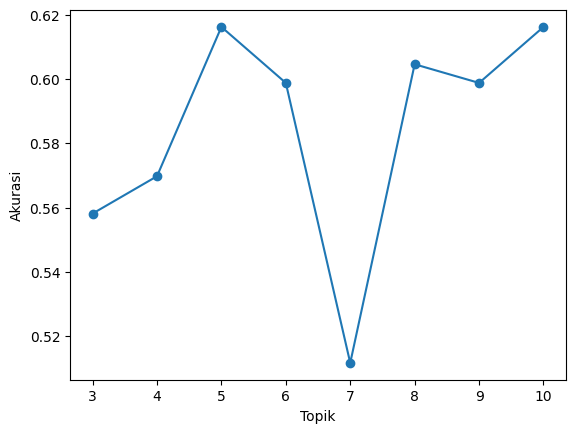
\includegraphics{LDA_Topic_Modelling_PTA_files/figure-pdf/cell-44-output-1.png}

}

\end{figure}

\bookmarksetup{startatroot}

\hypertarget{ekstraksi-kata-kunci}{%
\chapter{Ekstraksi Kata Kunci}\label{ekstraksi-kata-kunci}}

\begin{itemize}
\tightlist
\item
  \textbf{NLTK} berfungsi fungsi untuk melakukan tugas-tugas seperti
  tokenisasi, stemming, lemmatization, analisis sentimen, pengenalan
  entitas, dan banyak lagi.
\item
  \textbf{Pandas} menyediakan cara yang efisien untuk mengelola dan
  menganalisis data tabular seperti dataframe.
\item
  \textbf{CountVectorizer} untuk melakukan ekstraksi fitur dalam bentuk
  term frequency.
\item
  \textbf{numpy} untuk array dan operasi matematika pada array.
\item
  \textbf{re} Ekspresi reguler digunakan untuk pencocokan pola string
  dan manipulasi teks.
\item
  \textbf{networkx} adalah pustaka Python yang digunakan untuk analisis
  jaringan atau graf.
\end{itemize}

\begin{Shaded}
\begin{Highlighting}[]
\ImportTok{import}\NormalTok{ nltk}
\ImportTok{import}\NormalTok{ pandas }\ImportTok{as}\NormalTok{ pd}
\ImportTok{from}\NormalTok{ sklearn.feature\_extraction.text }\ImportTok{import}\NormalTok{ CountVectorizer}
\ImportTok{import}\NormalTok{ numpy }\ImportTok{as}\NormalTok{ np}
\ImportTok{import}\NormalTok{ matplotlib.pyplot }\ImportTok{as}\NormalTok{ plt}
\ImportTok{import}\NormalTok{ re}
\ImportTok{import}\NormalTok{ networkx }\ImportTok{as}\NormalTok{ nx}
\ImportTok{from}\NormalTok{ nltk.tokenize }\ImportTok{import}\NormalTok{ word\_tokenize}
\ImportTok{from}\NormalTok{ nltk.corpus }\ImportTok{import}\NormalTok{ stopwords}
\NormalTok{nltk.download(}\StringTok{\textquotesingle{}stopwords\textquotesingle{}}\NormalTok{)}
\NormalTok{nltk.download(}\StringTok{\textquotesingle{}punkt\textquotesingle{}}\NormalTok{)}
\end{Highlighting}
\end{Shaded}

\begin{verbatim}
[nltk_data] Downloading package stopwords to /root/nltk_data...
[nltk_data]   Package stopwords is already up-to-date!
[nltk_data] Downloading package punkt to /root/nltk_data...
[nltk_data]   Package punkt is already up-to-date!
\end{verbatim}

\begin{verbatim}
True
\end{verbatim}

\begin{Shaded}
\begin{Highlighting}[]
\CommentTok{\# Memanggil Dataset}
\NormalTok{data }\OperatorTok{=}\NormalTok{ pd.read\_csv(}\StringTok{"/content/drive/MyDrive/ppw/ppw/crawling\_berita\_pb.csv"}\NormalTok{)}
\NormalTok{data}
\end{Highlighting}
\end{Shaded}

\begin{longtable}[]{@{}llll@{}}
\toprule\noalign{}
& Judul & Isi & Kategori \\
\midrule\noalign{}
\endhead
\bottomrule\noalign{}
\endlastfoot
0 & Erik Ten Hag Tolak \textquotesingle Bejek\textquotesingle{} Skuad
Setan Merah U... & POJOKBACA.ID -PelatihManchester United(MU)Eri... &
Sport \\
1 & Muhaimin Minta Jokowi Adil di Pilpres 2024: Is... & JAKARTA,
POJOKBACA.ID -Bakal calon wakil pres... & Politik \\
2 & Sedang Bermain dan Berbagi Peran, Megawati-Jok... & JAKARTA,
POJOKBACA.ID -Polemik politik tanah a... & Politik \\
3 & Prabowo Subianto Kunjungi SBY Sebelum Daftar C... & BOGOR,
POJOKBACA.ID- Ketua Umum Partai Gerind... & Politik \\
4 & Universitas Gunadarma Ciptakan Robot Catur Cap... & JAKARTA,
POJOKBACA.ID-- Robot Catur benar-bena... & Sport \\
... & ... & ... & ... \\
431 & Ketua Umum Pro Jokowi: Prabowo - Gibran Akan M... & SOLO,
POJOKBACA.ID -Ketua Umum ProJokowi(Proj... & Politik \\
432 & Ganjar-Mahfud Didukung Ratusan Pedagang Pasar,... & MATARAM,
POJOKBACA.ID -Ratusan pedagang canan... & Politik \\
433 & PLN Unit Induk Distribusi Jakarta Raya Gelar A... & JAKARTA,
POJOKBACA.ID- Gelaran sepakbola akba... & Sport \\
434 & Jadwal Siaran langsung Timnas Indonesia U-17 d... & POJOKBACA.ID
-PadaPiala Dunia U-172023,Timnas... & Sport \\
435 & Jangan Biarkan HP Anda Cepat Panas dan Lowbet,... & POJOKBACA.ID
-HPatau handphone adalah alat ko... & Teknologi \\
\end{longtable}

\begin{Shaded}
\begin{Highlighting}[]
\CommentTok{\# Memberikan nomer pada dokumen}
\NormalTok{data[}\StringTok{\textquotesingle{}Dokumen ke\textquotesingle{}}\NormalTok{] }\OperatorTok{=}\NormalTok{ data.reset\_index(drop}\OperatorTok{=}\VariableTok{True}\NormalTok{).index }\OperatorTok{+} \DecValTok{1}
\NormalTok{data}
\end{Highlighting}
\end{Shaded}

\begin{longtable}[]{@{}lllll@{}}
\toprule\noalign{}
& Judul & Isi & Kategori & Dokumen ke \\
\midrule\noalign{}
\endhead
\bottomrule\noalign{}
\endlastfoot
0 & Erik Ten Hag Tolak \textquotesingle Bejek\textquotesingle{} Skuad
Setan Merah U... & POJOKBACA.ID -PelatihManchester United(MU)Eri... &
Sport & 1 \\
1 & Muhaimin Minta Jokowi Adil di Pilpres 2024: Is... & JAKARTA,
POJOKBACA.ID -Bakal calon wakil pres... & Politik & 2 \\
2 & Sedang Bermain dan Berbagi Peran, Megawati-Jok... & JAKARTA,
POJOKBACA.ID -Polemik politik tanah a... & Politik & 3 \\
3 & Prabowo Subianto Kunjungi SBY Sebelum Daftar C... & BOGOR,
POJOKBACA.ID- Ketua Umum Partai Gerind... & Politik & 4 \\
4 & Universitas Gunadarma Ciptakan Robot Catur Cap... & JAKARTA,
POJOKBACA.ID-- Robot Catur benar-bena... & Sport & 5 \\
... & ... & ... & ... & ... \\
431 & Ketua Umum Pro Jokowi: Prabowo - Gibran Akan M... & SOLO,
POJOKBACA.ID -Ketua Umum ProJokowi(Proj... & Politik & 432 \\
432 & Ganjar-Mahfud Didukung Ratusan Pedagang Pasar,... & MATARAM,
POJOKBACA.ID -Ratusan pedagang canan... & Politik & 433 \\
433 & PLN Unit Induk Distribusi Jakarta Raya Gelar A... & JAKARTA,
POJOKBACA.ID- Gelaran sepakbola akba... & Sport & 434 \\
434 & Jadwal Siaran langsung Timnas Indonesia U-17 d... & POJOKBACA.ID
-PadaPiala Dunia U-172023,Timnas... & Sport & 435 \\
435 & Jangan Biarkan HP Anda Cepat Panas dan Lowbet,... & POJOKBACA.ID
-HPatau handphone adalah alat ko... & Teknologi & 436 \\
\end{longtable}

\begin{Shaded}
\begin{Highlighting}[]
\CommentTok{\# Memanggil dokumen dengan nomer yang digunakan sebagai percobaan}
\NormalTok{data\_2 }\OperatorTok{=}\NormalTok{ data[data[}\StringTok{\textquotesingle{}Dokumen ke\textquotesingle{}}\NormalTok{] }\OperatorTok{==} \DecValTok{2}\NormalTok{]}
\NormalTok{data\_2}
\end{Highlighting}
\end{Shaded}

\begin{longtable}[]{@{}lllll@{}}
\toprule\noalign{}
& Judul & Isi & Kategori & Dokumen ke \\
\midrule\noalign{}
\endhead
\bottomrule\noalign{}
\endlastfoot
1 & Muhaimin Minta Jokowi Adil di Pilpres 2024: Is... & JAKARTA,
POJOKBACA.ID -Bakal calon wakil pres... & Politik & 2 \\
\end{longtable}

\hypertarget{tokenize-kalimat}{%
\section{Tokenize Kalimat}\label{tokenize-kalimat}}

\begin{Shaded}
\begin{Highlighting}[]
\CommentTok{\# membuat list untuk hasil tokenize}
\NormalTok{hasil\_kalimat}\OperatorTok{=}\NormalTok{[]}
\CommentTok{\# Melakukan perulangan untuk memisahkan berita per{-}kalimat}
\ControlFlowTok{for}\NormalTok{ i }\KeywordTok{in} \BuiltInTok{range}\NormalTok{(}\BuiltInTok{len}\NormalTok{(data\_2)):}
\NormalTok{  token }\OperatorTok{=}\NormalTok{ sent\_tokenize(data[}\StringTok{\textquotesingle{}Isi\textquotesingle{}}\NormalTok{][i])}
\NormalTok{  hasil\_kalimat.append(token)}
\end{Highlighting}
\end{Shaded}

\begin{Shaded}
\begin{Highlighting}[]
\CommentTok{\# membuat list untuk hasil transpose tokenize sebelumnya}
\NormalTok{kalimat }\OperatorTok{=}\NormalTok{ []}
\CommentTok{\# melakukan perulangan untuk merubah hasil tokenize / transpose data}
\ControlFlowTok{for}\NormalTok{ i }\KeywordTok{in} \BuiltInTok{range}\NormalTok{(}\BuiltInTok{len}\NormalTok{(hasil\_kalimat)):}
  \ControlFlowTok{for}\NormalTok{ x }\KeywordTok{in} \BuiltInTok{range}\NormalTok{ (}\BuiltInTok{len}\NormalTok{(hasil\_kalimat[i])):}
\NormalTok{    datacek }\OperatorTok{=}\NormalTok{ []}
\NormalTok{    datacek.append(i)}
\NormalTok{    datacek.append(hasil\_kalimat[i][x])}
\NormalTok{    kalimat.append(datacek)}
\CommentTok{\# kalimat}
\end{Highlighting}
\end{Shaded}

\begin{Shaded}
\begin{Highlighting}[]
\NormalTok{databaru }\OperatorTok{=}\NormalTok{ pd.DataFrame(kalimat, columns}\OperatorTok{=}\NormalTok{[}\StringTok{\textquotesingle{}Dokumen ke\textquotesingle{}}\NormalTok{,}\StringTok{\textquotesingle{}kalimat\textquotesingle{}}\NormalTok{])}
\NormalTok{databaru.loc[:, }\StringTok{\textquotesingle{}Dokumen ke\textquotesingle{}}\NormalTok{] }\OperatorTok{=} \DecValTok{2}
\CommentTok{\# databaru}
\end{Highlighting}
\end{Shaded}

\hypertarget{cleansing-2}{%
\section{Cleansing}\label{cleansing-2}}

\begin{Shaded}
\begin{Highlighting}[]
\CommentTok{\#Remove Puncutuation tidak termasuk menghapus spasi}
\CommentTok{\# menghilangkan Tag (@)}
\NormalTok{clean\_tag }\OperatorTok{=}\NormalTok{ re.}\BuiltInTok{compile}\NormalTok{(}\StringTok{\textquotesingle{}@\textbackslash{}S+\textquotesingle{}}\NormalTok{)}
\CommentTok{\# menghilangkan url (https?:\textbackslash{}/\textbackslash{}/)}
\NormalTok{clean\_url }\OperatorTok{=}\NormalTok{ re.}\BuiltInTok{compile}\NormalTok{(}\StringTok{\textquotesingle{}https?:\textbackslash{}/\textbackslash{}/.*[}\CharTok{\textbackslash{}r\textbackslash{}n}\StringTok{]*\textquotesingle{}}\NormalTok{)}
\CommentTok{\# menghilangkan hastag (\#)}
\NormalTok{clean\_hastag }\OperatorTok{=}\NormalTok{ re.}\BuiltInTok{compile}\NormalTok{(}\StringTok{\textquotesingle{}\#\textbackslash{}S+\textquotesingle{}}\NormalTok{)}
\CommentTok{\# menghilangkan simbol (\^{}a{-}zA{-}Z)}
\NormalTok{clean\_symbol }\OperatorTok{=}\NormalTok{ re.}\BuiltInTok{compile}\NormalTok{(}\StringTok{\textquotesingle{}[\^{}a{-}zA{-}Z]\textquotesingle{}}\NormalTok{)}
\KeywordTok{def}\NormalTok{ clean\_punct(text):}
\NormalTok{    text }\OperatorTok{=}\NormalTok{ clean\_tag.sub(}\StringTok{\textquotesingle{}\textquotesingle{}}\NormalTok{, }\BuiltInTok{str}\NormalTok{(text))}
\NormalTok{    text }\OperatorTok{=}\NormalTok{ clean\_url.sub(}\StringTok{\textquotesingle{}\textquotesingle{}}\NormalTok{, text)}
\NormalTok{    text }\OperatorTok{=}\NormalTok{ clean\_hastag.sub(}\StringTok{\textquotesingle{} \textquotesingle{}}\NormalTok{, text)}
\NormalTok{    text }\OperatorTok{=}\NormalTok{ clean\_symbol.sub(}\StringTok{\textquotesingle{} \textquotesingle{}}\NormalTok{, text)}
    \ControlFlowTok{return}\NormalTok{ text}
\CommentTok{\# Buat kolom tambahan untuk data description yang telah diremovepunctuation}
\NormalTok{preprocessing }\OperatorTok{=}\NormalTok{ data\_2[}\StringTok{\textquotesingle{}Isi\textquotesingle{}}\NormalTok{].}\BuiltInTok{apply}\NormalTok{(clean\_punct)}
\NormalTok{clean}\OperatorTok{=}\NormalTok{pd.DataFrame(preprocessing)}
\NormalTok{clean}
\end{Highlighting}
\end{Shaded}

\begin{longtable}[]{@{}ll@{}}
\toprule\noalign{}
& Isi \\
\midrule\noalign{}
\endhead
\bottomrule\noalign{}
\endlastfoot
1 & JAKARTA POJOKBACA ID Bakal calon wakil pres... \\
\end{longtable}

\hypertarget{tokenize-stopword-removal}{%
\section{Tokenize Stopword Removal}\label{tokenize-stopword-removal}}

\begin{itemize}
\tightlist
\item
  Dilakukan proses tokenisasi setiap kalimat.
\item
  Hasil tokenisasi dilakukan penghapusan kata yang tidak penting
\end{itemize}

\begin{Shaded}
\begin{Highlighting}[]
\CommentTok{\# Unduh stop words dari nltk}
\NormalTok{stop\_words }\OperatorTok{=} \BuiltInTok{set}\NormalTok{(stopwords.words(}\StringTok{\textquotesingle{}indonesian\textquotesingle{}}\NormalTok{))}
\CommentTok{\# Fungsi untuk menghapus stop words dari setiap kalimat}
\KeywordTok{def}\NormalTok{ remove\_stopwords(sentence):}
\NormalTok{    words }\OperatorTok{=}\NormalTok{ word\_tokenize(sentence)}
\NormalTok{    filtered\_words }\OperatorTok{=}\NormalTok{ [word }\ControlFlowTok{for}\NormalTok{ word }\KeywordTok{in}\NormalTok{ words }\ControlFlowTok{if}\NormalTok{ word.lower() }\KeywordTok{not} \KeywordTok{in}\NormalTok{ stop\_words]}
    \ControlFlowTok{return} \StringTok{\textquotesingle{} \textquotesingle{}}\NormalTok{.join(filtered\_words)}

\CommentTok{\# Terapkan fungsi pada kolom \textquotesingle{}Kalimat\textquotesingle{} dalam DataFrame}
\NormalTok{stopword }\OperatorTok{=}\NormalTok{ clean[}\StringTok{\textquotesingle{}Isi\textquotesingle{}}\NormalTok{].}\BuiltInTok{apply}\NormalTok{(remove\_stopwords)}
\NormalTok{stopword }\OperatorTok{=}\NormalTok{pd.DataFrame(stopword)}
\NormalTok{stopword}
\end{Highlighting}
\end{Shaded}

\begin{longtable}[]{@{}ll@{}}
\toprule\noalign{}
& Isi \\
\midrule\noalign{}
\endhead
\bottomrule\noalign{}
\endlastfoot
1 & JAKARTA POJOKBACA ID calon wakil presidenMuhai... \\
\end{longtable}

\hypertarget{co-occurrence-matriks}{%
\section{Co-Occurrence Matriks}\label{co-occurrence-matriks}}

Matriks co-occurrence (co-occurrence matrix) adalah suatu representasi
statistik dari hubungan antara dua atau lebih elemen dalam suatu
himpunan data. Ide dasarnya adalah untuk mengukur seberapa sering suatu
pasangan elemen muncul bersama-sama dalam suatu kumpulan data.

\begin{Shaded}
\begin{Highlighting}[]
\CommentTok{\# Menghitung matriks co{-}occurrence dengan CountVectorizer}
\NormalTok{vectorizer }\OperatorTok{=}\NormalTok{ CountVectorizer()}
\NormalTok{co\_occurrence\_matrix }\OperatorTok{=}\NormalTok{ vectorizer.fit\_transform(clean[}\StringTok{\textquotesingle{}Isi\textquotesingle{}}\NormalTok{]).T }\OperatorTok{*}\NormalTok{ vectorizer.fit\_transform(clean[}\StringTok{\textquotesingle{}Isi\textquotesingle{}}\NormalTok{])}

\CommentTok{\# Membuat DataFrame dari matriks co{-}occurrence}
\NormalTok{df\_co\_occurrence }\OperatorTok{=}\NormalTok{ pd.DataFrame(co\_occurrence\_matrix.toarray(), columns}\OperatorTok{=}\NormalTok{vectorizer.get\_feature\_names\_out(),index}\OperatorTok{=}\NormalTok{vectorizer.get\_feature\_names\_out())}
\NormalTok{df\_co\_occurrence}
\end{Highlighting}
\end{Shaded}

\begin{longtable}[]{@{}llllllllllllllllllllll@{}}
\toprule\noalign{}
& acara & akan & anaknya & anies & antara & baca & bahwa & bakal &
bangsa & bantai & ... & ummat & umum & untuk & usai & wakil & wib &
widodo & wormuth & yakni & yang \\
\midrule\noalign{}
\endhead
\bottomrule\noalign{}
\endlastfoot
acara & 1 & 2 & 2 & 3 & 1 & 3 & 1 & 6 & 2 & 1 & ... & 1 & 2 & 1 & 1 & 2
& 1 & 2 & 1 & 2 & 1 \\
akan & 2 & 4 & 4 & 6 & 2 & 6 & 2 & 12 & 4 & 2 & ... & 2 & 4 & 2 & 2 & 4
& 2 & 4 & 2 & 4 & 2 \\
anaknya & 2 & 4 & 4 & 6 & 2 & 6 & 2 & 12 & 4 & 2 & ... & 2 & 4 & 2 & 2 &
4 & 2 & 4 & 2 & 4 & 2 \\
anies & 3 & 6 & 6 & 9 & 3 & 9 & 3 & 18 & 6 & 3 & ... & 3 & 6 & 3 & 3 & 6
& 3 & 6 & 3 & 6 & 3 \\
antara & 1 & 2 & 2 & 3 & 1 & 3 & 1 & 6 & 2 & 1 & ... & 1 & 2 & 1 & 1 & 2
& 1 & 2 & 1 & 2 & 1 \\
... & ... & ... & ... & ... & ... & ... & ... & ... & ... & ... & ... &
... & ... & ... & ... & ... & ... & ... & ... & ... & ... \\
wib & 1 & 2 & 2 & 3 & 1 & 3 & 1 & 6 & 2 & 1 & ... & 1 & 2 & 1 & 1 & 2 &
1 & 2 & 1 & 2 & 1 \\
widodo & 2 & 4 & 4 & 6 & 2 & 6 & 2 & 12 & 4 & 2 & ... & 2 & 4 & 2 & 2 &
4 & 2 & 4 & 2 & 4 & 2 \\
wormuth & 1 & 2 & 2 & 3 & 1 & 3 & 1 & 6 & 2 & 1 & ... & 1 & 2 & 1 & 1 &
2 & 1 & 2 & 1 & 2 & 1 \\
yakni & 2 & 4 & 4 & 6 & 2 & 6 & 2 & 12 & 4 & 2 & ... & 2 & 4 & 2 & 2 & 4
& 2 & 4 & 2 & 4 & 2 \\
yang & 1 & 2 & 2 & 3 & 1 & 3 & 1 & 6 & 2 & 1 & ... & 1 & 2 & 1 & 1 & 2 &
1 & 2 & 1 & 2 & 1 \\
\end{longtable}

Pembentukan Graph : Setiap kata yang memiliki hubungan dengan kata lain
dan nilai Term frequency lebih dari 5 akan dibentuk node yang saling
terhubung

\hypertarget{pagerank}{%
\section{Pagerank}\label{pagerank}}

\textbf{TextRank} adalah suatu algoritma ekstraksi rangking teks yang
digunakan untuk mengekstrak informasi utama atau rangkuman dari suatu
teks. Algoritma ini didasarkan pada konsep PageRank, yang awalnya
dikembangkan oleh Google untuk menilai kualitas dan relevansi halaman
web dalam hasil pencarian. TextRank digunakan dalam konteks pemrosesan
bahasa alami dan pengolahan teks. Sehingga dari penjelasan tersebut
Textrank digunakan untuk mencari kata paling penting dalam sebuah
dokumen.

Dalam kasus kali ini PageRank mengukur otoritas atau kepentingan suatu
kata berdasarkan seberapa banyak kata lain yang mengaitkan ke kata
tersebut dan seberapa pentingnya kata-kata yang memberikan tautan
tersebut.

\hypertarget{algoritma-textrank}{%
\subsection{\texorpdfstring{\textbf{Algoritma
Textrank}}{Algoritma Textrank}}\label{algoritma-textrank}}

\begin{enumerate}
\def\labelenumi{\arabic{enumi}.}
\tightlist
\item
  Tokenisasi (Teks awal dibagi menjadi token atau unit-unit teks yang
  lebih kecil)
\item
  Pembobotan Kata / Co-Occurrence Matriks (Setiap kata atau frasa diberi
  bobot berdasarkan karakteristik tertentu)
\item
  Membangun Graf Berbobot (Kata-kata atau frasa dinyatakan sebagai
  simpul dalam graf, dan hubungan antara mereka dinyatakan sebagai tepi)
\item
  TextRank (Algoritma PageRank digunakan untuk menghitung skor
  keterkaitan atau signifikansi dari setiap simpul dalam graf. Dalam
  konteks TextRank, simpul yang mendapatkan skor tertinggi dianggap
  sebagai kata-kata atau frasa yang paling penting.)
\end{enumerate}

dikarenakan konsep dari Textrank sama dengan Pagerank maka rumus
Pagerank dapat digunakan untuk menghitung Textrank.

\textbf{Rumus Pagerank :}

\(\text{PR(A)}=\frac{d}{N} + \left( 1 - d\right)\left( \sum_{}^{} \frac{\text{Rank(i)}}{Outlink(i)} \right)\)

\begin{itemize}
\tightlist
\item
  PR(i) adalah PageRank dari kata A
\item
  d adalah faktor damping (biasanya 0.85 untuk Google PageRank)
\item
  N adalah jumlah total kata
\end{itemize}

\hypertarget{contoh-manual-pagerank}{%
\subsection{\texorpdfstring{\textbf{Contoh manual
Pagerank}}{Contoh manual Pagerank}}\label{contoh-manual-pagerank}}

https://docs.google.com/spreadsheets/d/1kGmqOQ2q3RcFOXFjrEiYRdj3qA8L7OLl/edit?usp=sharing\&ouid=102642560487377842579\&rtpof=true\&sd=true

\begin{Shaded}
\begin{Highlighting}[]
\NormalTok{G }\OperatorTok{=}\NormalTok{ nx.DiGraph()}
\ControlFlowTok{for}\NormalTok{ idx, row }\KeywordTok{in}\NormalTok{ df\_co\_occurrence.iterrows():}
    \ControlFlowTok{for}\NormalTok{ col }\KeywordTok{in}\NormalTok{ df\_co\_occurrence.columns:}
\NormalTok{        weight }\OperatorTok{=}\NormalTok{ df\_co\_occurrence.loc[idx, col]}
        \ControlFlowTok{if}\NormalTok{ weight }\OperatorTok{\textgreater{}} \DecValTok{30} \KeywordTok{and}\NormalTok{ idx }\OperatorTok{!=}\NormalTok{ col:}
\NormalTok{            G.add\_edge(idx, col, weight}\OperatorTok{=}\NormalTok{weight)}
\end{Highlighting}
\end{Shaded}

\begin{Shaded}
\begin{Highlighting}[]
\CommentTok{\# Menampilkan graf}
\NormalTok{pos }\OperatorTok{=}\NormalTok{ nx.spring\_layout(G)}
\NormalTok{labels }\OperatorTok{=}\NormalTok{ nx.get\_edge\_attributes(G, }\StringTok{\textquotesingle{}weight\textquotesingle{}}\NormalTok{)}
\NormalTok{nx.draw(G, pos, with\_labels}\OperatorTok{=}\VariableTok{True}\NormalTok{, node\_size}\OperatorTok{=}\DecValTok{700}\NormalTok{, node\_color}\OperatorTok{=}\StringTok{\textquotesingle{}skyblue\textquotesingle{}}\NormalTok{, font\_size}\OperatorTok{=}\DecValTok{10}\NormalTok{, font\_color}\OperatorTok{=}\StringTok{\textquotesingle{}black\textquotesingle{}}\NormalTok{, arrowsize}\OperatorTok{=}\DecValTok{20}\NormalTok{)}
\NormalTok{nx.draw\_networkx\_edge\_labels(G, pos, edge\_labels}\OperatorTok{=}\NormalTok{labels)}
\NormalTok{plt.title(}\StringTok{"Co{-}occurrence Directed Graph"}\NormalTok{)}
\NormalTok{plt.show()}
\end{Highlighting}
\end{Shaded}

\begin{figure}[H]

{\centering 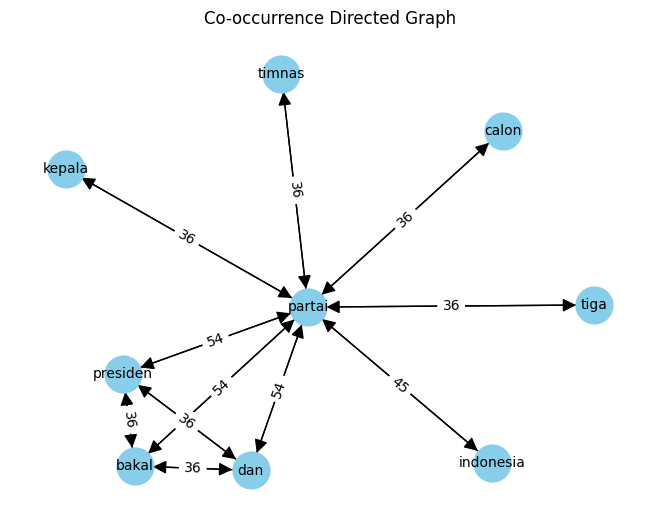
\includegraphics{Ektraksi_Kata_Kunci_files/figure-pdf/cell-13-output-1.png}

}

\end{figure}

\begin{Shaded}
\begin{Highlighting}[]
\NormalTok{pr }\OperatorTok{=}\NormalTok{ nx.pagerank(G)}
\NormalTok{sorted\_d }\OperatorTok{=} \BuiltInTok{sorted}\NormalTok{(pr.items(), key}\OperatorTok{=}\KeywordTok{lambda}\NormalTok{ x: x[}\DecValTok{1}\NormalTok{], reverse}\OperatorTok{=}\VariableTok{True}\NormalTok{)[:}\DecValTok{4}\NormalTok{]}
\NormalTok{sorted\_d}
\end{Highlighting}
\end{Shaded}

\begin{verbatim}
[('partai', 0.36903524863219894),
 ('bakal', 0.12624278988303878),
 ('dan', 0.12624278988303878),
 ('presiden', 0.12624278988303878)]
\end{verbatim}

\begin{Shaded}
\begin{Highlighting}[]
\CommentTok{\# Hitung centrality pada berita 1 dengan closeness}
\NormalTok{closeness\_centrality }\OperatorTok{=}\NormalTok{ nx.closeness\_centrality(G)}
\CommentTok{\# Ubah ke dalam dataframe}
\NormalTok{closeness\_df }\OperatorTok{=}\NormalTok{ pd.DataFrame(}\BuiltInTok{list}\NormalTok{(closeness\_centrality.items()), columns}\OperatorTok{=}\NormalTok{[}\StringTok{\textquotesingle{}Kata\textquotesingle{}}\NormalTok{, }\StringTok{\textquotesingle{}Closeness Centrality\textquotesingle{}}\NormalTok{])}
\NormalTok{closeness\_df }\OperatorTok{=}\NormalTok{ closeness\_df.sort\_values(by}\OperatorTok{=}\StringTok{\textquotesingle{}Closeness Centrality\textquotesingle{}}\NormalTok{, ascending}\OperatorTok{=}\VariableTok{False}\NormalTok{)}
\NormalTok{closeness\_df}
\end{Highlighting}
\end{Shaded}

\begin{longtable}[]{@{}lll@{}}
\toprule\noalign{}
& Kata & Closeness Centrality \\
\midrule\noalign{}
\endhead
\bottomrule\noalign{}
\endlastfoot
2 & partai & 1.000000 \\
0 & bakal & 0.615385 \\
1 & dan & 0.615385 \\
3 & presiden & 0.615385 \\
4 & calon & 0.533333 \\
5 & indonesia & 0.533333 \\
6 & kepala & 0.533333 \\
7 & tiga & 0.533333 \\
8 & timnas & 0.533333 \\
\end{longtable}



\backmatter
\printindex

\end{document}
